% Options for packages loaded elsewhere
\PassOptionsToPackage{unicode}{hyperref}
\PassOptionsToPackage{hyphens}{url}
\PassOptionsToPackage{dvipsnames,svgnames,x11names}{xcolor}
\documentclass[
  10pt,
  a4paper,
  krantz2]{krantz}
\usepackage{xcolor}
\usepackage{amsmath,amssymb}
\setcounter{secnumdepth}{5}
\usepackage{iftex}
\ifPDFTeX
  \usepackage[T1]{fontenc}
  \usepackage[utf8]{inputenc}
  \usepackage{textcomp} % provide euro and other symbols
\else % if luatex or xetex
  \usepackage{unicode-math} % this also loads fontspec
  \defaultfontfeatures{Scale=MatchLowercase}
  \defaultfontfeatures[\rmfamily]{Ligatures=TeX,Scale=1}
\fi
\usepackage{lmodern}
\ifPDFTeX\else
  % xetex/luatex font selection
\fi
% Use upquote if available, for straight quotes in verbatim environments
\IfFileExists{upquote.sty}{\usepackage{upquote}}{}
\IfFileExists{microtype.sty}{% use microtype if available
  \usepackage[]{microtype}
  \UseMicrotypeSet[protrusion]{basicmath} % disable protrusion for tt fonts
}{}
\makeatletter
\@ifundefined{KOMAClassName}{% if non-KOMA class
  \IfFileExists{parskip.sty}{%
    \usepackage{parskip}
  }{% else
    \setlength{\parindent}{0pt}
    \setlength{\parskip}{6pt plus 2pt minus 1pt}}
}{% if KOMA class
  \KOMAoptions{parskip=half}}
\makeatother
\usepackage{color}
\usepackage{fancyvrb}
\newcommand{\VerbBar}{|}
\newcommand{\VERB}{\Verb[commandchars=\\\{\}]}
\DefineVerbatimEnvironment{Highlighting}{Verbatim}{commandchars=\\\{\}}
% Add ',fontsize=\small' for more characters per line
\usepackage{framed}
\definecolor{shadecolor}{RGB}{248,248,248}
\newenvironment{Shaded}{\begin{snugshade}}{\end{snugshade}}
\newcommand{\AlertTok}[1]{\textcolor[rgb]{0.33,0.33,0.33}{#1}}
\newcommand{\AnnotationTok}[1]{\textcolor[rgb]{0.37,0.37,0.37}{\textbf{\textit{#1}}}}
\newcommand{\AttributeTok}[1]{\textcolor[rgb]{0.27,0.27,0.27}{#1}}
\newcommand{\BaseNTok}[1]{\textcolor[rgb]{0.06,0.06,0.06}{#1}}
\newcommand{\BuiltInTok}[1]{#1}
\newcommand{\CharTok}[1]{\textcolor[rgb]{0.5,0.5,0.5}{#1}}
\newcommand{\CommentTok}[1]{\textcolor[rgb]{0.37,0.37,0.37}{\textit{#1}}}
\newcommand{\CommentVarTok}[1]{\textcolor[rgb]{0.37,0.37,0.37}{\textbf{\textit{#1}}}}
\newcommand{\ConstantTok}[1]{\textcolor[rgb]{0.37,0.37,0.37}{#1}}
\newcommand{\ControlFlowTok}[1]{\textcolor[rgb]{0.27,0.27,0.27}{\textbf{#1}}}
\newcommand{\DataTypeTok}[1]{\textcolor[rgb]{0.27,0.27,0.27}{#1}}
\newcommand{\DecValTok}[1]{\textcolor[rgb]{0.06,0.06,0.06}{#1}}
\newcommand{\DocumentationTok}[1]{\textcolor[rgb]{0.37,0.37,0.37}{\textbf{\textit{#1}}}}
\newcommand{\ErrorTok}[1]{\textcolor[rgb]{0.14,0.14,0.14}{\textbf{#1}}}
\newcommand{\ExtensionTok}[1]{#1}
\newcommand{\FloatTok}[1]{\textcolor[rgb]{0.06,0.06,0.06}{#1}}
\newcommand{\FunctionTok}[1]{\textcolor[rgb]{0.27,0.27,0.27}{\textbf{#1}}}
\newcommand{\ImportTok}[1]{#1}
\newcommand{\InformationTok}[1]{\textcolor[rgb]{0.37,0.37,0.37}{\textbf{\textit{#1}}}}
\newcommand{\KeywordTok}[1]{\textcolor[rgb]{0.27,0.27,0.27}{\textbf{#1}}}
\newcommand{\NormalTok}[1]{#1}
\newcommand{\OperatorTok}[1]{\textcolor[rgb]{0.43,0.43,0.43}{\textbf{#1}}}
\newcommand{\OtherTok}[1]{\textcolor[rgb]{0.37,0.37,0.37}{#1}}
\newcommand{\PreprocessorTok}[1]{\textcolor[rgb]{0.37,0.37,0.37}{\textit{#1}}}
\newcommand{\RegionMarkerTok}[1]{#1}
\newcommand{\SpecialCharTok}[1]{\textcolor[rgb]{0.43,0.43,0.43}{\textbf{#1}}}
\newcommand{\SpecialStringTok}[1]{\textcolor[rgb]{0.5,0.5,0.5}{#1}}
\newcommand{\StringTok}[1]{\textcolor[rgb]{0.5,0.5,0.5}{#1}}
\newcommand{\VariableTok}[1]{\textcolor[rgb]{0,0,0}{#1}}
\newcommand{\VerbatimStringTok}[1]{\textcolor[rgb]{0.5,0.5,0.5}{#1}}
\newcommand{\WarningTok}[1]{\textcolor[rgb]{0.37,0.37,0.37}{\textbf{\textit{#1}}}}
\usepackage{longtable,booktabs,array}
\usepackage{calc} % for calculating minipage widths
% Correct order of tables after \paragraph or \subparagraph
\usepackage{etoolbox}
\makeatletter
\patchcmd\longtable{\par}{\if@noskipsec\mbox{}\fi\par}{}{}
\makeatother
% Allow footnotes in longtable head/foot
\IfFileExists{footnotehyper.sty}{\usepackage{footnotehyper}}{\usepackage{footnote}}
\makesavenoteenv{longtable}
\usepackage{graphicx}
\makeatletter
\newsavebox\pandoc@box
\newcommand*\pandocbounded[1]{% scales image to fit in text height/width
  \sbox\pandoc@box{#1}%
  \Gscale@div\@tempa{\textheight}{\dimexpr\ht\pandoc@box+\dp\pandoc@box\relax}%
  \Gscale@div\@tempb{\linewidth}{\wd\pandoc@box}%
  \ifdim\@tempb\p@<\@tempa\p@\let\@tempa\@tempb\fi% select the smaller of both
  \ifdim\@tempa\p@<\p@\scalebox{\@tempa}{\usebox\pandoc@box}%
  \else\usebox{\pandoc@box}%
  \fi%
}
% Set default figure placement to htbp
\def\fps@figure{htbp}
\makeatother
% definitions for citeproc citations
\NewDocumentCommand\citeproctext{}{}
\NewDocumentCommand\citeproc{mm}{%
  \begingroup\def\citeproctext{#2}\cite{#1}\endgroup}
\makeatletter
 % allow citations to break across lines
 \let\@cite@ofmt\@firstofone
 % avoid brackets around text for \cite:
 \def\@biblabel#1{}
 \def\@cite#1#2{{#1\if@tempswa , #2\fi}}
\makeatother
\newlength{\cslhangindent}
\setlength{\cslhangindent}{1.5em}
\newlength{\csllabelwidth}
\setlength{\csllabelwidth}{3em}
\newenvironment{CSLReferences}[2] % #1 hanging-indent, #2 entry-spacing
 {\begin{list}{}{%
  \setlength{\itemindent}{0pt}
  \setlength{\leftmargin}{0pt}
  \setlength{\parsep}{0pt}
  % turn on hanging indent if param 1 is 1
  \ifodd #1
   \setlength{\leftmargin}{\cslhangindent}
   \setlength{\itemindent}{-1\cslhangindent}
  \fi
  % set entry spacing
  \setlength{\itemsep}{#2\baselineskip}}}
 {\end{list}}
\usepackage{calc}
\newcommand{\CSLBlock}[1]{\hfill\break\parbox[t]{\linewidth}{\strut\ignorespaces#1\strut}}
\newcommand{\CSLLeftMargin}[1]{\parbox[t]{\csllabelwidth}{\strut#1\strut}}
\newcommand{\CSLRightInline}[1]{\parbox[t]{\linewidth - \csllabelwidth}{\strut#1\strut}}
\newcommand{\CSLIndent}[1]{\hspace{\cslhangindent}#1}
\setlength{\emergencystretch}{3em} % prevent overfull lines
\providecommand{\tightlist}{%
  \setlength{\itemsep}{0pt}\setlength{\parskip}{0pt}}
\usepackage{booktabs}

\usepackage{longtable}
\usepackage[bf,singlelinecheck=off]{caption}
\usepackage{times,pifont} % Nice fonts
%\usepackage[x11names]{xcolor}
\usepackage{fancyhdr}
\usepackage{amsbsy}
\usepackage[T1]{fontenc}


%  Configure listings package for R code (you can customize this further)
\usepackage{listings} % For the lstlisting environment
\lstset{
  language=R, % Set default language to R
  basicstyle=\ttfamily\scriptsize, % Font style and size
  frame=single, % Single frame around the listing
  backgroundcolor=\color{gray!10}, % Light grey background
  breaklines=true, % Break long lines
  showstringspaces=false, % Don't show special characters for spaces
  commentstyle=\color{gray!50}, % Example: style comments
  keywordstyle=\color{blue!70!black}, % Example: style keywords
  stringstyle=\color{red!70!black}, % Example: style strings
  numbers=none, % No line numbers
  %numbersep=5pt, % Space between line numbers and code
}

% Format R chunks from ```{r}:
\definecolor{keywordcolor}{RGB}{0,0,150}
\definecolor{commentcolor}{RGB}{0,150,0}
\definecolor{stringcolor}{RGB}{150,0,0}

%\renewcommand{\KeywordTok}[1]{\textcolor{keywordcolor}{#1}}
%\renewcommand{\CommentTok}[1]{\textcolor{commentcolor}{#1}}
%\renewcommand{\StringTok}[1]{\textcolor{stringcolor}{#1}}

% \renewcommand{\KeywordTok}[1]{\textcolor[rgb]{0.00,0.44,0.13}{\textbf{{#1}}}}
% \renewcommand{\DataTypeTok}[1]{\textcolor[rgb]{0.56,0.13,0.00}{{#1}}}
% \renewcommand{\DecValTok}[1]{\textcolor[rgb]{0.25,0.63,0.44}{{#1}}}
% \renewcommand{\BaseNTok}[1]{\textcolor[rgb]{0.25,0.63,0.44}{{#1}}}
% \renewcommand{\FloatTok}[1]{\textcolor[rgb]{0.25,0.63,0.44}{{#1}}}
% \renewcommand{\CharTok}[1]{\textcolor[rgb]{0.25,0.44,0.63}{{#1}}}
% \renewcommand{\StringTok}[1]{\textcolor[rgb]{0.25,0.44,0.63}{{#1}}}
% \renewcommand{\CommentTok}[1]{\textcolor[rgb]{0.38,0.63,0.69}{\textit{{#1}}}}
% \renewcommand{\OtherTok}[1]{\textcolor[rgb]{0.00,0.44,0.13}{{#1}}}
% \renewcommand{\AlertTok}[1]{\textcolor[rgb]{1.00,0.00,0.00}{\textbf{{#1}}}}
% \renewcommand{\FunctionTok}[1]{\textcolor[rgb]{0.02,0.16,0.49}{{#1}}}
% \renewcommand{\RegionMarkerTok}[1]{{#1}}
% \renewcommand{\ErrorTok}[1]{\textcolor[rgb]{1.00,0.00,0.00}{\textbf{{#1}}}}
% \renewcommand{\NormalTok}[1]{{#1}}

\renewcommand{\KeywordTok}[1]{\textcolor[rgb]{0.00,0.00,0.7}{\textbf{{#1}}}}
\renewcommand{\DataTypeTok}[1]{\textcolor[rgb]{0.56,0.13,0.00}{{#1}}}
\renewcommand{\DecValTok}[1]{\textcolor[rgb]{0.25,0.63,0.44}{{#1}}}
\renewcommand{\BaseNTok}[1]{\textcolor[rgb]{0.25,0.63,0.44}{{#1}}}
\renewcommand{\FloatTok}[1]{\textcolor[rgb]{0.25,0.63,0.44}{{#1}}}
\renewcommand{\CharTok}[1]{\textcolor[rgb]{0.25,0.44,0.63}{{#1}}}
\renewcommand{\StringTok}[1]{\textcolor[rgb]{0.7,0, 0}{{#1}}}
\renewcommand{\CommentTok}[1]{\textcolor[rgb]{0.65,0.65,0.65}{\textit{{#1}}}}
\renewcommand{\OtherTok}[1]{\textcolor[rgb]{0.00,0.44,0.13}{{#1}}}
\renewcommand{\AlertTok}[1]{\textcolor[rgb]{1.00,0.00,0.00}{\textbf{{#1}}}}
\renewcommand{\FunctionTok}[1]{\textcolor[rgb]{0.02,0.16,0.79}{\textbf{{#1}}}}
\renewcommand{\RegionMarkerTok}[1]{{#1}}
\renewcommand{\ErrorTok}[1]{\textcolor[rgb]{1.00,0.00,0.00}{\textbf{{#1}}}}
\renewcommand{\NormalTok}[1]{{#1}}




\usepackage{customdice} % Help with die unicode!

\usepackage{tabularx} % For column specifications, using the kable_styling function  column_spec()
\usepackage{tabu} % For column specifications, using the kable_styling function  column_spec()
\usepackage{float} % Needed for some kableExtra stuff
\usepackage{mdframed}
\usepackage{enumitem} % To change the itemize spacing in exercises.
\usepackage{subfig} % For sub-figure captions
\usepackage[font={small,it}]{caption}
\usepackage{wrapfig} % For text-wrapping figures

\usepackage{enumitem}% http://ctan.org/pkg/enumitem. Remove some space between itemie are preceeding text
\setlist[itemize]{noitemsep, topsep=1pt}

% FIGURE PLACEMENT: https://tex.stackexchange.com/questions/140568/how-to-set-default-positioning-of-figure-table-document-wide
\makeatletter
  \providecommand*\setfloatlocations[2]{\@namedef{fps@#1}{#2}}
\makeatother
\setfloatlocations{figure}{hbtp}
\setfloatlocations{table}{hbtp}


%\setmainfont[UprightFeatures={SmallCapsFont=AlegreyaSC-Regular}]{Alegreya}

\usepackage{framed,color}
\definecolor{shadecolor}{RGB}{245,245,245}
\definecolor{lightshadecolor}{RGB}{230, 230, 255}
\definecolor{textcolor}{RGB}{100,100,100}

%\definecolor{exampleExtraColor}{RGB}{209, 223, 250}
\definecolor{examplecolor}{RGB}{245, 245, 245}

\renewcommand{\textfraction}{0.05}
\renewcommand{\topfraction}{0.8}
\renewcommand{\bottomfraction}{0.8}
\renewcommand{\floatpagefraction}{0.75}


% In HTML, < gets rendered as &lt; in table headers etc. So I defined the command \lt and \gt to use:
\newcommand{\lt}{\ensuremath{<}}
\newcommand{\gt}{\ensuremath{>}}

%\renewenvironment{quote}{\begin{VF}}{\end{VF}}
\renewenvironment{quote}%
  {\begin{kframe}}
  {\end{kframe}}



% Redo the  href  command
%\let\oldhref\href
%\renewcommand{\href}[2]{#2\footnote{\textbf{\url{#1}}}}

% \ifxetex
%   \usepackage{letltxmacro}
%   \setlength{\XeTeXLinkMargin}{1pt}
%   \LetLtxMacro\SavedIncludeGraphics\includegraphics
%   \def\includegraphics#1#{% #1 catches optional stuff (star/opt. arg.)
%     \IncludeGraphicsAux{#1}%
%   }%
%   \newcommand*{\IncludeGraphicsAux}[2]{%
%     \XeTeXLinkBox{%
%       \SavedIncludeGraphics#1{#2}%
%     }%
%   }%
% \fi

% Default figure width
\setkeys{Gin}{width=0.5\linewidth}


\makeatletter
\newenvironment{kframe}{%
\medskip{}
\setlength{\fboxsep}{.8em}
 \def\at@end@of@kframe{}%
 \ifinner\ifhmode%
  \def\at@end@of@kframe{\end{minipage}}%
  \begin{minipage}{\columnwidth}%
 \fi\fi%
 \def\FrameCommand##1{\hskip\@totalleftmargin \hskip-\fboxsep
 \colorbox{shadecolor}{##1}\hskip-\fboxsep
     % There is no \\@totalrightmargin, so:
     \hskip-\linewidth \hskip-\@totalleftmargin \hskip\columnwidth}%
 \MakeFramed {\advance\hsize-\width
   \@totalleftmargin\z@ \linewidth\hsize
   \@setminipage}}%
 {\par\unskip\endMakeFramed%
 \at@end@of@kframe}
 \makeatother
 




% \newenvironment{rmdthinkHTML}{}{} % DO nothing

\newenvironment{rmdblock}[1]
  {\setlength{\itemindent}{10em}\begin{quote}\vspace{-1em}
  \begin{itemize}\setlength{\parskip}{2mm}
  \renewcommand{\labelitemi}{
    \raisebox{-.5\height}[0pt][0pt]{
      {\setkeys{Gin}{width=1.5em,keepaspectratio}\includegraphics{icons/#1}}
    }
  }
  \setlength{\fboxsep}{1em}
  \begin{kframe}
  \item
  } % END START ENV
  {% BEGIN END ENV
  \end{kframe}
  \end{itemize}\vspace{-0.75em}\end{quote}
  }
\newenvironment{rmdblockNoIcon}
  {\begin{quote}\vspace{-0.75em}
  \setlength{\parskip}{2mm}
  %\begin{kframe}
  }
  {%\end{kframe}
  \vspace{-0.05em}\end{quote}
  }
  


\usepackage{tcolorbox} % Provides  \newtcolorbox

%%% Objectives boxes
\definecolor{ObjColour}{RGB}{237, 233, 251}
\newtcolorbox{objectivescolourbox}{
  colback=ObjColour,
  colframe=ObjColour,
  coltext=black,
  boxsep=5pt,
  arc=4pt}

\newenvironment{objectivesBox}[1]
  {
  \begin{itemize}[leftmargin=.5in]\small
  \renewcommand{\labelitemi}{
    \raisebox{-.4\height}[0pt][0pt]{
      {\setkeys{Gin}{width=1.5em,keepaspectratio}
        \includegraphics{icons/#1}\qquad}
    }
  }
  \setlength{\fboxsep}{1em}
  \begin{objectivescolourbox}
  \item
  }
  {
  \end{objectivescolourbox}
  \end{itemize}
  }  
  
  

% Tip boxes
\definecolor{TipColour}{rgb}{0.965, 0.996, 0.898}
\newtcolorbox{tipcolourbox}{
  colback=TipColour,
  colframe=TipColour,
  coltext=black,
  boxsep=5pt,
  arc=4pt}

  
\newenvironment{tipBox}[1]
  {
  \begin{itemize}[leftmargin=.5in]
  \renewcommand{\labelitemi}{
    \raisebox{-.4\height}[0pt][0pt]{
      {\setkeys{Gin}{width=1.5em,keepaspectratio}
        \includegraphics{icons/#1}\qquad}
    }
  }
  \setlength{\fboxsep}{1em}
  \begin{tipcolourbox}
  \item
  }
  {
  \end{tipcolourbox}
  \end{itemize}
  }
  


% Link boxes
\definecolor{LinkColour}{rgb}{0.965, 0.996, 0.898}
\newtcolorbox{linkcolourbox}{
  colback=LinkColour,
  colframe=LinkColour,
  coltext=black,
  boxsep=5pt,
  arc=4pt}

  
\newenvironment{linkBox}[1]
  {
  \begin{itemize}[leftmargin=.5in]
  \renewcommand{\labelitemi}{
    \raisebox{-.4\height}[0pt][0pt]{
      {\setkeys{Gin}{width=1.5em,keepaspectratio}
        \includegraphics{icons/#1}\qquad}
    }
  }
  \setlength{\fboxsep}{1em}
  \begin{linkcolourbox}
  \item
  }
  {
  \end{linkcolourbox}
  \end{itemize}
  }
  
  
  
    
% Important Box
\definecolor{ImportantColour}{rgb}{0.996, 0.934, 0.898}
\newtcolorbox{importantcolourbox}{
  colback=ImportantColour,
  colframe=ImportantColour,
  coltext=black,
  boxsep=5pt,
  arc=4pt}
\newenvironment{importantBox}[1]
  {\vspace{2mm}
  \begin{itemize}[leftmargin=.5in]
  \renewcommand{\labelitemi}{
    \raisebox{-.4\height}[0pt][0pt]{
      {\setkeys{Gin}{width=1.5em,keepaspectratio}
        \includegraphics{icons/#1}\qquad}
    }
  }
  \setlength{\fboxsep}{1em}
  \begin{importantcolourbox}\setlength{\parskip}{2mm}
  \item
  }
  {
  \end{importantcolourbox}
  \end{itemize}
  } 


% Software Box
\definecolor{SoftwareColour}{rgb}{0.898, 0.945, 0.996}
\newtcolorbox{softwarecolourbox}{
  colback=SoftwareColour,
  colframe=SoftwareColour,
  coltext=black,
  boxsep=5pt,
  arc=4pt}
\newenvironment{softwareBox}[1]
  {
  \begin{itemize}[leftmargin=.5in]
  \renewcommand{\labelitemi}{
    \raisebox{-.4\height}[0pt][0pt]{
      {\setkeys{Gin}{width=1.5em,keepaspectratio}
        \includegraphics{icons/#1}\qquad}
    }
  }
  \setlength{\fboxsep}{1em}
  \begin{softwarecolourbox}\setlength{\parskip}{2mm}
  \item
  }
  {
  \end{softwarecolourbox}
  \end{itemize}
  } 






% Think Box
\definecolor{ThinkColour}{RGB}{247, 255, 230}
\newtcolorbox{thinkcolourbox}{
  colback=ThinkColour,
  colframe=ThinkColour,
  coltext=black,
  boxsep=5pt,
  arc=4pt}
\newenvironment{thinkBox}[1]
  {
  \begin{itemize}[leftmargin=.5in]
  \renewcommand{\labelitemi}{
    \raisebox{-.4\height}[0pt][0pt]{
      {\setkeys{Gin}{width=1.5em,keepaspectratio}
        \includegraphics{icons/#1}\qquad}
    }
  }
  \setlength{\fboxsep}{1em}
  \begin{thinkcolourbox}\setlength{\parskip}{2mm}
  \item
  }
  {
  \end{thinkcolourbox}
  \end{itemize}
  } 



% Pronounce Box
\definecolor{PronounceColour}{RGB}{249, 242, 236}
\newtcolorbox{pronouncecolourbox}{
  colback = PronounceColour,
  colframe = PronounceColour,
  coltext = black,
  boxsep = 5pt,
  arc = 4pt}
\newenvironment{pronounceBox}[1]
  {
  \begin{itemize}[leftmargin=.5in]
  \renewcommand{\labelitemi}{
    \raisebox{-.4\height}[0pt][0pt]{
      {\setkeys{Gin}{width=1.5em,keepaspectratio}
        \includegraphics{icons/#1}\qquad}
    }
  }
  \setlength{\fboxsep}{1em}
  \begin{pronouncecolourbox}
  \item
  }
  {
  \end{pronouncecolourbox}
  \end{itemize}
  } 




% Progress Box: Should be blank (i.e. nothing appears) for LaTeX as it is not dynamic
\AtBeginEnvironment{progressBox}{\begin{comment}}
\AtEndEnvironment{progressBox}{\end{comment}}
\definecolor{ProgressColour}{rgb}{0.996, 0.996, 0.797}
\newtcolorbox{progresscolourbox}{
  colback = ProgressColour,
  colframe = ProgressColour,
  coltext = black,
  boxsep = 5pt,
  arc = 4pt}
\newenvironment{progressBox}[1]
  {}
  {}


% SRM:
%\newenvironment{answer}
%  {\footnotesize}
%  {\null\vspace{-5mm}} %{\smallskip}


\newenvironment{answer}
  {\null\vspace{-2mm}\footnotesize}
  {\null\vspace{-2mm}} %{\smallskip}

\newenvironment{rmdnote}
  {\begin{rmdblock}{iconmonstr-light-bulb-2-240}}
  {\end{rmdblock}}
  
% exampleExtra: Omit this is latex
\usepackage{comment}
\excludecomment{exampleExtra}
%\newenvironment{exampleExtra}{}{}
%  {\begin{rmdblock}{iconmonstr-idea-12-240}\small\textbf{Example.}}
%  {\begin{rmdblockNoIcon}\small\textbf{Extra example:}}
%  {\end{rmdblockNoIcon}}



\newenvironment{darkgraytext}{\color{textcolor}}{\ignorespacesafterend}
%\AtBeginEnvironment{rmdblockNoIcon}{\begin{comment}}
%\AtEndEnvironment{rmdblockNoIcon}{\end{comment}}

%\usepackage{amsthm}
%\newtheorem*{ExampleFold}{Example}


%%% TRY HIDING EXAMPLE FOLDS, EXAMPLE FOLDS: To save paper in printing...???



% Redfine some existing environments
% -QUOTE
\makeatletter
\renewenvironment{quote}
               {\list{}{\vspace{-0.5em}\begin{kframe}\small%
                        \itemindent    \listparindent
                        \rightmargin   \leftmargin
                        \parsep        \z@ \@plus\p@}%
                \item\relax}
               {\end{kframe}\endlist}
\makeatother


% ORIGINAL:
%\newenvironment{fold}
%  {\begin{rmdblock}{iconmonstr-idea-12-240}\vspace{-1em}\begin{darkgraytext}\footnotesize \textbf{Answer:}}
%  {\end{darkgraytext}\end{rmdblock}}
%\newenvironment{fold}
%  {\vspace{-6pt}\begin{rmdblockNoIcon}\scriptsize \textbf{Answer:}}
%  {\end{rmdblockNoIcon}}
  
% Change the  fold  environment to be disappeared
% Note: In the LaTeX code, it appears like this: \BeginKnitrBlock{fold}
%\usepackage{comment}
%\AtBeginEnvironment{fold}{\begin{comment}}
%\AtEndEnvironment{fold}{\end{comment}}

%\begin{shaded}}
%\AtEndEnvironment{fold}{\end{shaded}}

%%% IF ONLY THIS WORKED:
% \usepackage{comment}
% \includecomment{fold}





\usepackage{url}
\urlstyle{sf}
     

\usepackage{imakeidx} % Add some pre-index text
\makeindex
\indexsetup{othercode=\footnotesize} % Change index font size


% NOTE:  clashes with  ntheorem  package... if I want to use that. I tried to use if to put lemma in shaded backgrounds... without luck. So I just put this code back.
\usepackage{amsthm}
\makeatletter
\def\thm@space@setup{%
  \thm@preskip=8pt plus 2pt minus 4pt
  \thm@postskip=\thm@preskip
}
\makeatother



% Background colour on defn and examples
\AtBeginDocument{%
\let\origendexample=\endexample%
\let\origexample=\example%

\renewenvironment{example}%
  {\begingroup\definecolor{shadecolor}{RGB}{232, 232, 232}\vspace{2mm}\begin{quote}\setlength{\parskip}{2mm}\vspace{-8mm}\origexample}%
  {\origendexample\end{quote}\vspace{2mm}\endgroup}}


\AtBeginDocument{%
\let\origenddefinition=\enddefinition%
\let\origdefinition=\definition%

\renewenvironment{definition}%
  {\begingroup\definecolor{shadecolor}{RGB}{242, 242, 242}\vspace{2mm}\begin{quote}\setlength{\parskip}{2mm}\vspace{-8mm}\origdefinition}%
  {\origenddefinition\end{quote}\vspace{-1mm}\endgroup\vspace{1mm}}}






\AtBeginDocument{%
\let\origendtheorem=\endtheorem%
\let\origtheorem=\theorem%
\renewenvironment{theorem}%
  {\begingroup\definecolor{shadecolor}{RGB}{245, 245, 245}\vspace{2mm}\begin{quote}\setlength{\parskip}{2mm}\vspace{-4mm}\origtheorem}%
  {\origendtheorem\end{quote}\vspace{-5mm}\endgroup\vspace{2mm}}}



%% TRY CHANGE R CODE FONT SIZE.
%%% FROM : https://stackoverflow.com/questions/38323331/code-chunk-font-size-in-beamer-with-knitr-and-latex
%% change fontsize of R code
\let\oldShaded\Shaded
\let\endoldShaded\endShaded
\renewenvironment{Shaded}{\footnotesize\oldShaded}{\endoldShaded}

%% change fontsize of output
\let\oldverbatim\verbatim
\let\endoldverbatim\endverbatim
\renewenvironment{verbatim}{\footnotesize\oldverbatim}{\endoldverbatim}


% Circled letters (e.g., Heads and Tails):
\usepackage{tikz}
\newcommand*\circled[1]{\tikz[baseline=(char.base)]{
            \node[shape=circle,draw,inner sep=0.8pt] (char) {{\textsc{#1}}};}}
\newcommand{\Heads}{\circled{h}}
\newcommand{\Tails}{\circled{t}}


% Format the R chunks
\lstdefinestyle{mycode}{
  language=R,
  basicstyle=\ttfamily\scriptsize,
  frame=single,
  backgroundcolor=\color{gray!10},
  commentstyle=\color{gray!50}\itshape,
  keywordstyle=\color{blue!70!black}\bfseries,
  stringstyle=\color{red!70!black},
  numbers=none,
  breaklines=true
}

\lstdefinestyle{myoutput}{
  basicstyle=\ttfamily\small,
  breaklines=true
}


\frontmatter


\newenvironment{cols}[1][]{}{}

\newenvironment{col}[1]{\begin{minipage}[t]{#1}\vspace{-6pt}\ignorespaces}{% % The \vspace seems needed, or image is not top aligned: https://tex.stackexchange.com/questions/580709/two-minipage-top-align-one-with-figure?rq=1
\end{minipage}
\ifhmode\unskip\fi
\aftergroup\useignorespacesandallpars}

\def\useignorespacesandallpars#1\ignorespaces\fi{%
#1\fi\ignorespacesandallpars}

\makeatletter
\def\ignorespacesandallpars{%
  \@ifnextchar\par
    {\expandafter\ignorespacesandallpars\@gobble}%
    {}%
}
\makeatother
\usepackage{bookmark}
\IfFileExists{xurl.sty}{\usepackage{xurl}}{} % add URL line breaks if available
\urlstyle{same}
% Make links footnotes instead of hotlinks:
\DeclareRobustCommand{\href}[2]{#2\footnote{\url{#1}}}
\hypersetup{
  pdftitle={The Theory of Statistical Distributions},
  pdfauthor={Peter K. Dunn},
  colorlinks=true,
  linkcolor={Maroon},
  filecolor={Maroon},
  citecolor={Blue},
  urlcolor={Blue},
  pdfcreator={LaTeX via pandoc}}

\title{The Theory of Statistical Distributions}
\author{Peter K. Dunn}
\date{Last updated: 2026-02-18}

\usepackage{amsthm}
\newtheorem{theorem}{Theorem}[chapter]
\newtheorem{lemma}{Lemma}[chapter]
\newtheorem{corollary}{Corollary}[chapter]
\newtheorem{proposition}{Proposition}[chapter]
\newtheorem{conjecture}{Conjecture}[chapter]
\theoremstyle{definition}
\newtheorem{definition}{Definition}[chapter]
\theoremstyle{definition}
\newtheorem{example}{Example}[chapter]
\theoremstyle{definition}
\newtheorem{exercise}{Exercise}[chapter]
\theoremstyle{definition}
\newtheorem{hypothesis}{Hypothesis}[chapter]
\theoremstyle{remark}
\newtheorem*{remark}{Remark}
\newtheorem*{solution}{Solution}
\begin{document}
\maketitle


% For CRC, according to `Run_This_Example.tex`:


\frontmatter

\title{Distribution Theory} %This is a placeholder titlepage, it will not be final.
\author{Peter K. Dunn}
%%%\maketitle

%%%Placeholder for front matter

%\halftitle

%\booktitle

%\locpage

%\include{frontmatter/dedication}
\cleardoublepage
\setcounter{page}{7} %previous pages will be reserved for frontmatter to be added in later.
%\tableofcontents
%\include{frontmatter/foreword}
%\include{frontmatter/preface}
%%\listoffigures
%%\listoftables
%\include{frontmatter/contributor}
%\include{frontmatter/symbollist}

\mainmatter




% WAS THIS:
%
% \thispagestyle{empty}
% 
% \setlength{\abovedisplayskip}{-5pt}
% \setlength{\abovedisplayshortskip}{-5pt}
% 
% 
% % Reinstate maketitle 
% % (https://stackoverflow.com/questions/45963505/coverpage-and-copyright-notice-before-title-in-r-bookdown):
% 
% %\makebox[\textwidth]{\includegraphics[width=\paperwidth]{OtherImages/cover.png}}
% %\let\maketitle\oldmaketitle
% %\maketitle
% 
% 
% % Fix the itemize/enumerate spacing in exercises:
% \let\origexercise=\exercise
% \def\exercise{\begingroup\setitemize{labelindent=1.5em,labelsep=3mm,leftmargin=*}\setenumerate{labelindent=1.5em,labelsep=3mm,leftmargin=*}\origexercise}  
%    %% -5mm removes some spacing at the top, which looked odd. Chosen by trial and error
% \let\origendexercise=\endexercise
% \def\endexercise{\origendexercise\endgroup}
%    %% \setitem  from the  enumitem  package
% 
% % Prepare chapter TOC
% %\dominitoc

\index{Three axioms of probability|see{Axioms of probability}}
\index{Probability axioms|see{Axioms of probability}}
\index{Kolmogorov's axioms of probability|see{Axioms of probability}}

\index{Relative frequency probability|see{Probability, relative frequency probability}}
\index{Empirical probability|see{Probability, relative frequency probability}}
\index{Classical probability|see{Probability, classical probability}}
\index{Subjective probability|see{Probability, subjective}}


\index{Probability density function|see{PDF}}
\index{Cumulative distribution function|see{Df}}
\index{Distribution function|see{Df}}

\index{Random experiment|see{Random process}}
\index{Event space|see{Sample space}}
\index{Outcome space|see{Sample space}}
\index{Null set|see{Empty set}}
\index{Outcome space|see{Sample space}}
\index{Sets, null|see{Null set}}
\index{Sets, universal|see{Universal set}}
\index{Disjoint sets|see{Sets, disjoint}}

\index{Elementary event|see{Events, simple}}
\index{Probability!axioms|see{Axioms of probability}}
\index{Conditional probability|see{Probability, conditional}}
\index{Reduced sample space|see{Sample space, reduced}}

\index{Range space|see{Range}}
\index{Value set|see{Range}}
\index{Range|seealso{Domain}}
\index{Domain|seealso{Range}}

\index{Distributions|seealso{Specific names of distributions}}
\index{Kurtosis|seealso{Playtkurtic}}
\index{Kurtosis|seealso{Leptokurtic}}
\index{Kurtosis|seealso{Mesokurtic}}
\index{Skewness|seealso{Symmetric}}
\index{MGF|see{Moment generating function}}

\index{Mean|seealso{Expected value}}
\index{Expected value|seealso{Mean}}

\index{Tweedie distributions|seealso{Compound Poisson--gamma distributions}}
\index{Compound Poisson--gamma distributions|seealso{Tweedie distributions}}


\index{Simple random sample|seealso{Sampling, simple random sample}}
\index{Random numbers|seealso{Pseudo-random numbers}}
\index{Pseudo-random numbers|seealso{Random numbers}}


{
\hypersetup{linkcolor=}
\setcounter{tocdepth}{1}
\tableofcontents
}
\newcommand{\cms}{\,\text{cm}}
\newcommand{\dLs}{\,\text{dL}}
\newcommand{\xdLs}{\text{dL}}

\newcommand{\fmols}{\,\text{fmol}}
\newcommand{\ft}{\,\text{ft}}
\newcommand{\gs}{\,\text{g}}
\newcommand{\hs}{\,\text{h}}
\newcommand{\xhs}{\text{h}}

\newcommand{\has}{\,\text{ha}}
\newcommand{\xhas}{\text{ha}}

\newcommand{\inches}{\,\text{inches}}
\newcommand{\kgs}{\,\text{kg}}
\newcommand{\kms}{\,\text{km}}
\newcommand{\kWhs}{\,\text{kWh}}
\newcommand{\lbs}{\,\text{lb}}
\newcommand{\Ls}{\,\text{L}}
\newcommand{\xLs}{\text{L}}

\newcommand{\mgs}{\,\text{mg}}
\newcommand{\microgs}{\,\ensuremath{\mu}\text{g}}
\newcommand{\millis}{\,\text{ms}}
\newcommand{\mins}{\,\text{mins}}
\newcommand{\mJs}{\,\text{mJ}}
\newcommand{\mmols}{\,\text{mmol}}
\newcommand{\mLs}{\,\text{mL}}
\newcommand{\mms}{\,\text{mm}}
\newcommand{\ms}{\,\text{m}}
\newcommand{\xms}{\text{m}}
\newcommand{\ozs}{\,\text{oz}}
\newcommand{\secs}{\,\text{s}}
\newcommand{\xsecs}{\text{s}}
\newcommand{\ppms}{\,\text{ppm}}
\newcommand{\ys}{\,\text{y}}
\newcommand{\vs}{\,\text{V}}

\frontmatter

\chapter*{Preface}\label{preface}


This book is an introduction to the theory of statistical probability and distributions.

\section*{Statistical software}\label{statistical-software}


This book can be read without relying on any specific statistical software, though sometimes \textbf{R} code (\citeproc{ref-R-base}{R Core Team 2024}) is included to demonstrate ideas, and to discuss simulation.

\section*{Callouts used on this book}\label{callouts-used-on-this-book}


The callouts used in this book have meanings; for example:

\begin{objectivesBox}{iconmonstr-target-4-240.png}
These chunks introduce the objectives for the chapters of the book.

\end{objectivesBox}

\begin{importantBox}{iconmonstr-warning-8-240.png}
These chunks highlight common mistakes or warnings, about a particular concept or about using a formula.

\end{importantBox}

\begin{tipBox}{iconmonstr-info-6-240.png}
These chunks offer helpful information.

\end{tipBox}

\begin{softwareBox}{iconmonstr-laptop-4-240.png}
These chunks refer to text that is relevant to using the \textbf{R} statistical software.

\end{softwareBox}

\begin{linkBox}{iconmonstr-link-1-240.png}
These chunks explain how certain concepts and distributions are linked.

\end{linkBox}

\begin{thinkBox}{iconmonstr-light-bulb-2-240.png}
These chunks give you some questions to think about.

\end{thinkBox}

\section*{Who can use this book?}\label{who-can-use-this-book}


This textbook is \textbf{free} for anyone to use:
There is no charge for students, instructors or institutions.

Although not essential, an email to the author (explaining how the textbook is being used, who is using the textbook, and your thoughts on the textbook) would be appreciated: \texttt{pdunn2\ \textless{}at\textgreater{}\ usc.edu.au}.

\section*{How this book was made}\label{how-this-book-was-made}


This book was made using \textbf{R} (\citeproc{ref-R-base}{R Core Team 2024}), and the \textbf{bookdown} package (\citeproc{ref-R-bookdown}{Y. Xie 2025a}), which is based on \href{https://en.wikipedia.org/wiki/Markdown}{Markdown} syntax, using \textbf{knitr} (\citeproc{ref-R-knitr}{Y. Xie 2025b}).

\section*{Learning Outcomes}\label{learning-outcomes}


\begin{objectivesBox}{iconmonstr-target-4-240.png}

In this book, you will learn to:

\begin{itemize}
\tightlist
\item
  apply rules, theorems and concepts to compute probabilities.
\item
  describe probability and distribution functions.
\item
  apply concepts of mathematical expectation.
\item
  apply and work with standard discrete and continuous distributions, including computing of probabilities.
\item
  apply and work with bivariate and multivariate distributions.
\item
  determine probability functions and distribution functions of transformed radon variables.
\item
  apply and work with standard sampling distributions.
\item
  use \textbf{R} to produce relevant plots and compute probabilities.
\end{itemize}

\end{objectivesBox}

\section*{How to cite this book}\label{how-to-cite-this-book}


Peter K. Dunn (2024). \emph{The theory of statistical distributions}.
\url{https://bookdown.org/pkaldunn/DistTheory}

The \href{https://creativecommons.org/licenses/by-nc-sa/4.0/}{CC BY-NC-SA 4.0} licence is applied to this textbook.

\begin{flushright}
Peter K. Dunn\\
Sippy Downs, Australia
\end{flushright}

\mainmatter

\chapter{Introduction}\label{ChapterIntroduction}

Imagine if life was deterministic!
The commute to the gym, university or work would always take exactly the same length of time; weather predictions would always be accurate; you would know exactly what lotto numbers would be drawn on the weekend\ldots{}

However, life is full of unpredictable variation.

Variation may be \emph{unpredictable}, but patterns still emerge.
We may not know what the next toss of a coin will produce\ldots{} but we see a \emph{pattern} in the long run: a Head appears about half the time.

\emph{Probability} is one of the tools used to describe and understand this unpredictability.
\emph{Distribution theory} is about describing the patterns in this unpredictability using \emph{probability}.
\emph{Statistics} is about data collection and extracting information from \emph{data}, using probability and distribution theory to make decisions based on the data.

In most fields of study, always being certain is almost impossible, and so probability is necessary:

\begin{itemize}
\tightlist
\item
  What is the chance that a particular share price will crash next month?
\item
  What are the odds that a medical patient will suffer from a dangerous side-effect?
\item
  How likely is it that a dam will overflow next year?
\item
  What is the chance of finding a rare bird species in a given forest?
\end{itemize}

To answer these questions, a framework is needed: concepts like \emph{probability} need defining, and notation and theory are required.
These tools are important for modelling real-world phenomena, but also for providing a firm mathematical foundation for the theory of statistics.

Computers and computer packages are essential tools in the application of statistics to real problems.
In this book, the statistical package \textbf{R} is used, and will be used to illustrate various concepts to help you understand the theory.

One way in which \textbf{R} can be used is to easily compute probabilities for specific distributions.
Also, \textbf{R} can be used to verify (not \emph{prove}) theoretical results obtained.
To do this, a technique called \emph{computer simulation} can be used.

Simulation can also be used to solve problems for which it may be difficult (or impossible) to obtain a theoretical result.
Sometimes these numerical solutions to intractable analytical problems is termed \emph{Monte Carlo simulation}.

\part{Theoretical foundations}\label{part-theoretical-foundations}

\chapter{Essentials of set theory}\label{ChapterSetTheory}

\begin{objectivesBox}{iconmonstr-target-4-240.png}

Upon completion of this chapter you should be able to:

\begin{itemize}
\tightlist
\item
  define sets, and define elements of sets.
\item
  define the cardinality of sets.
\item
  perform basic set operations.
\end{itemize}

\end{objectivesBox}

\section{Introduction to sets}\label{Sets}

The basis of probability is working with \emph{sets}, which we first define.
Informally, a \emph{set} is a collection of objects.

\begin{definition}[Set]
\protect\hypertarget{def:Sets}{}\label{def:Sets}A \emph{set}\index{Set} is a well-defined, unordered collection of distinct \emph{elements}.\index{Elements of sets}
\end{definition}

In this definition:

\begin{itemize}
\tightlist
\item
  `distinct' means that an element is either present or absent in the set; there is no concept of repeated elements in a set.
\item
  `unordered' means that the order of the elements in the set is irrelevant.
\item
  `well-defined' means that it must be clear whether any object belongs to the set or does not belong to the set.
\end{itemize}

Sets are usually denoted using a capital letter, such as \(A\).
Sets can be finite, countably infinite, or uncountable; the distinctions are discussed further in Sect.~\ref{FiniteInfiniteSets}.

For some sets, listing the individual elements is possible:
\[
   A = \{ a_1, a_2, a_3, a_4\},
\]
when we can write \(a_2\in A\) to indicate that~\(a_2\) is an element of the set~\(A\).
However, listing the elements like this is not always possible (e.g., for uncountably infinite sets).

Set \emph{elements}\index{Elements of sets} can be interpreted broadly, and can refer to letters, digits, names, suits in a pack of cards, numbers, words, animals, people, machine components, plants\ldots{} or even other sets.

\begin{example}[Sets]
\protect\hypertarget{exm:DefineSets}{}\label{exm:DefineSets}Consider these two sets:
\begin{align*}
  A &= \{\text{Brisbane}, \text{Sydney}, \text{Hobart}, \text{Melbourne}, \text{Adelaide}, \text{Perth}\};\\
  B &= \{\text{Hobart}, \text{Melbourne}, \text{Perth, }\text{Brisbane}, \text{Sydney}, \text{Adelaide}\}.
\end{align*}
These two sets are \emph{equal}, since the order of the elements does not matter: both sets contain six distinct elements (`Australian state capital cities').
We can write \(A = B\).

In contrast,
\[
  C = \{\text{Brisbane}, \text{Sydney}, \text{Hobart}, \text{Sydney}, \text{Hobart}, \text{Hobart} \}
\]
contains redundancy; the elements `Sydney' and `Hobart' are repeated.
By definition, repeated elements in sets are redundant, so~\(C\) is equivalent to writing
\[
  C = \{\text{Brisbane}, \text{Sydney}, \text{Hobart} \}.
\]
\end{example}

\begin{example}[Examples of sets]
\protect\hypertarget{exm:ExamplesOfSets}{}\label{exm:ExamplesOfSets}Define the set~\(M\) as:
\[
  M = \{\text{Echidnas}, \text{Platypuses}\},
\]
\(M\) is the set of all known monotremes.
Set~\(M\) has two elements.

Also, define the set~\(D\) as
\[
   D = \{1, 3, 5, 7, 9\},
\]
the set of all even digits.
Set~\(D\) has five elements.

Then, we could define the set~\(W\) as:
\[
  W = \{ M, D\} = \{ (\text{Echidnas}, \text{Platypuses}), (1, 3, 5, 7, 9)\}.
\]
The set~\(W\) contains two elements: the sets~\(M\) and~\(D\).
\end{example}

The symbol `\(\in\)' is used to denote that an element is a member of a set; the symbol `\(\notin\)' is used to denote that an element is \emph{not} a member of a set.
If \(a\) is an element of the set \(A\), we write \(a \in A\), and we say `\(a\) is an element of set~\(A\)'.

\begin{example}[Elements of sets]
\protect\hypertarget{exm:DefineSetsIn}{}\label{exm:DefineSetsIn}For set~\(A\) in Example~\ref{exm:DefineSets}, we can write
\[
  \text{Hobart} \in A
\]
to indicate that `Hobart' is a member of set~\(A\).
Similarly, we can write
\[
  \text{Canberra} \notin A
\]
to indicate that `Canberra' is \emph{not} a member of~\(A\).
\end{example}

\section{Defining the elements of sets}\label{DescribingElementsOfSets}

Elements\index{Elements of sets!defining} of a set can be defined in several ways:

\begin{itemize}
\tightlist
\item
  \emph{Enumerating}: listing all the individual elements.
\item
  \emph{Description}: specifying a property that all elements share.
\item
  \emph{Using a rule}: defining a precise condition that determines set membership.
\end{itemize}

Regardless of the method used, any given object must be clearly a member of the set or not a member of the set.

\begin{example}[Elements in a set]
\protect\hypertarget{exm:DefineSetsElements}{}\label{exm:DefineSetsElements}Set~\(A\) in Example~\ref{exm:DefineSets} lists its elements explicitly.
Alternatively, \(A\) could be defined by a \emph{description}, by stating `the set of capital cities in Australian states'.

`Canberra' is \emph{not} an element of~\(A\), since Canberra is not an Australia state capital.
\end{example}

\begin{example}[Defining elements of a set]
\protect\hypertarget{exm:DefiningSets2}{}\label{exm:DefiningSets2}Define the set \(L\) as `all books at the local library with more than two authors'.
Listing all elements is impractical, but the rule clearly determines membership: any book either satisfies the condition (and belongs to~\(L\)) or does not.
\end{example}

\section{Specific sets}\label{SpecialSets}

Some sets are standard in mathematics and probability, and have special names or symbols.

\begin{definition}[Empty set]
\protect\hypertarget{def:EmptySet}{}\label{def:EmptySet}The \emph{null set}, or the \emph{empty set},\index{Empty set} has no elements, and is denoted by \(\varnothing\).
\end{definition}

\begin{importantBox}{iconmonstr-warning-8-240.png}
The \emph{set} itself is denoted \(\varnothing\), which contains zero elements.

\end{importantBox}

\begin{definition}[Universal set]
\protect\hypertarget{def:UniversalSet}{}\label{def:UniversalSet}The \emph{universal set}\index{Universal set} is the set of all elements under consideration in a specific context.
It is often denoted by \(S\), \(U\) or \(\Omega\).
\end{definition}

\begin{example}[Universal sets]
\protect\hypertarget{exm:universalSet}{}\label{exm:universalSet}The universal set is the set of all objects currently under discussion, so it depends on context.

If we are talking about people in a room, \(U\) is the set of all people in the room.
If we are talking about integers, \(U\) is the set of all integers.
If we are talking about dealing cards, \(U\) is the set of all cards in the pack.
\end{example}

In practice, a universal is almost always defined.
Theoretically, unrestricted universal sets lead to paradoxes such as \emph{Russell's paradox}.\index{Russell's paradox}

\begin{tipBox}{iconmonstr-info-6-240.png}
Russell's paradox,\index{Russell's paradox} discovered by Bertrand Russell in~1901, arises from considering this set:
\[
   R = \{ \text{all sets that are \textbf{not} members of themselves} \}.
\]
Then:

\begin{itemize}
\tightlist
\item
  If \(R\in R\), then (by definition) \(R\notin R\), which is a contradiction.
\item
  If \(R\notin R\), then (by definition) \(R\in R\), which is a contradiction.
\end{itemize}

Both cases lead to a contradiction.
Modern set theory (such as ZFC)\index{ZFC} restricts sets formation to avoid such paradoxes.

\end{tipBox}

\begin{example}[Null set]
\protect\hypertarget{exm:NullSet}{}\label{exm:NullSet}Consider rolling a standard six-sided die
The \emph{universal set} is
\[
  U = \{1, 2, 3, 4, 5, 6\}.
\]
The set of rolls greater than~\(4\) is
\[
  B = \{5, 6\}.
\]
The set of rolls greater than~\(10\) contains \emph{no} elements, and so
\[
  C = \varnothing.
\]
We do not write \(C = \{\varnothing\}\); the symbol \(\varnothing\) itself represents a set (with no elements).
Writing
\[
  C = \{\varnothing\},
\]
defines~\(C\) as a set with one element, and that element is the empty set.
\end{example}

Some commonly used sets of numbers include:

\begin{itemize}
\tightlist
\item
  \emph{Natural} (or counting) numbers\index{Number sets!natural} \(\mathbb{N}\): \(\{1, 2, 3, \dots\}\).
\item
  \emph{Integers}\index{Number sets!integers} \(\mathbb{Z}\): \(\{\ldots, -2, 1, 0, 1, 2, 3, \dots\}\).
\item
  \emph{Rational}\index{Number sets!rationals} numbers \(\mathbb{Q}\), including numbers like \(1/2 = 0.5\).
\item
  \emph{Real}\index{Number sets!reals} numbers \(\mathbb{R}\), including numbers like \(\pi\).
\item
  \emph{Positive real}\index{Number sets!positive reals} numbers \(\mathbb{R}_{+}\).
\item
  \emph{Negative real}\index{Number sets!negative reals} numbers \(\mathbb{R}_{-}\).
\item
  \emph{Complex}\index{Number sets!complex} numbers \(\mathbb{C}\).
\end{itemize}

(Some authors include~\(0\) in the set of natural numbers.)

\section{Cardinality of sets}\label{FiniteInfiniteSets}

Sets can be:\index{Cardinality}

\begin{itemize}
\tightlist
\item
  \emph{finite}, where elements can be counted; the number of elements~\(n\) is finite.
\item
  \emph{countable infinite}: elements could be listed in a sequence, but there are infinitely many.
\item
  \emph{uncountably infinite}: elements cannot all be listed in a sequence.
\end{itemize}

For finite or countably infinite sets, each element is called an \emph{element} or a \emph{sample point}.

\subsection{Finite sets}\label{FiniteSets}

If\index{Finite sets}\index{Cardinality!Finite sets} the number of elements in a set can be counted, the set is called a \emph{finite} set.
A finite set has exactly~\(n\) distinct elements for some non-negative integer~\(n\).

\begin{example}[Defining elements of a set]
\protect\hypertarget{exm:DefiningSets3}{}\label{exm:DefiningSets3}Define set \(A\) as
\[
   A = \left\{ \text{Countries whose names begin and end with the letter A}\right\}.
\]
The elements of \(A\) include, for example, `Austria', `Antigua and Barbuda' and `Albania'.
\(A\) contains a \emph{finite} number of elements.
\end{example}

\begin{example}[Defining elements of a finite sets]
\protect\hypertarget{exm:DefiningSets}{}\label{exm:DefiningSets}Define the set \(S\) as the `set of suits in a standard pack of cards'.
Then, \(S = \{\clubsuit, \spadesuit, \heartsuit, \diamondsuit\}\).
We can write, for example, that \(\spadesuit \in S\).

The elements of the set are listed; the set has four elements.
\end{example}

\begin{example}[Defining elements of a finite sets]
\protect\hypertarget{exm:DefiningSets4}{}\label{exm:DefiningSets4}Define the set~\(O\) as the `set of odd numbers between~\(0\) and~\(100\)'.
Alternatively, the elements of the set can defined by giving the pattern:
\[
  O = \{1, 3, 5, 7, 9, \dots 95, 97, 99\}
\]
Set~\(O\) has \(50\)~elements.
\end{example}

\begin{example}[Finite sets]
\protect\hypertarget{exm:FiniteSets}{}\label{exm:FiniteSets}Define set \(B\) as `the even numbers after rolling a single die'; then,

\[
  B = \big\{
   \largedice{2},
   \largedice{4},
   \largedice{6} \big\}.
\]

The set~\(B\) is \emph{finite}, with three elements.
\end{example}

\subsection{Countably infinite sets}\label{CountablyInfiniteSets}

If\index{Countably infinite sets}\index{Cardinality!Countably infinite} the elements in a set could (in principle) be listed without omitting any element, but an infinite number of them exist, the set is called a \emph{countably finite} set.

\begin{definition}[Countably infinite set]
\protect\hypertarget{def:CountablyInfiniteSets}{}\label{def:CountablyInfiniteSets}A set is called \emph{countably infinite} if its elements can be put into a one-to-one correspondence with the natural numbers
\[
  N = \{1, 2, 3, \dots\}.
\]
Each element appears exactly once in the sequence.
\end{definition}

\begin{example}[Countably infinite sets]
\protect\hypertarget{exm:DefiningSets5}{}\label{exm:DefiningSets5}Define \(S\) as the number of rolls of a die needed to roll a
\largedice{6}.
The number of rolls needed could be \(1\) or \(2\) or \(3\)\ldots, and no upper limit exists (though some numbers are very unlikely).
That is, the set~\(S\) is
\[
  S = \{1, 2, 3, 4, \dots\}
\]
Set~\(S\) is \emph{countably infinite}.
\end{example}

\begin{example}[Countably infinite sets]
\protect\hypertarget{exm:DefiningSets6}{}\label{exm:DefiningSets6}Define the set \(O\) as the `set of odd numbers'.
The elements of the set can be described (`odd numbers'), or by giving the pattern:
\[
  O = \{1, 3, 5, 7, 9, \dots\}
\]
Set~\(O\) is \emph{countably infinite}.
\end{example}

\subsection{Uncountably infinite sets}\label{InfiniteSets}

If\index{Uncountably infinite sets}\index{Cardinality!Uncountably infinite sets} the elements cannot be listed without omitting elements, the set is called a \emph{uncountably finite} set.

\begin{definition}[Uncountably infinite sets]
\protect\hypertarget{def:UncountablyInfiniteSets}{}\label{def:UncountablyInfiniteSets}A set is \emph{uncountably infinite} if its elements cannot be listed in a sequence without missing some elements.
\end{definition}

\begin{example}[Uncountably infinite sets]
\protect\hypertarget{exm:UncountablyInfiniteSets}{}\label{exm:UncountablyInfiniteSets}The set \(\mathbb{R}\) refers to the positive real numbers, which is an \emph{uncountably infinite} set.
The elements of \(\mathbb{R}\) cannot be listed without missing some elements.
For instance, an infinite number of elements exists between the elements~\(0\) and~\(0.0001\).

Set~\(\mathbb{R}\) is \emph{uncountably infinite}.
\end{example}

\begin{example}[Uncountably infinite set]
\protect\hypertarget{exm:HeightsOfPeople}{}\label{exm:HeightsOfPeople}Consider the heights of people.
Between the two heights \(173\,\text{cm}\) and \(174\,\text{cm}\), an infinite number of heights exist:
\(173.1\,\text{cm}\), \(173.01\,\text{cm}\), \(173.001\,\text{cm}\), \(173.0001\,\text{cm}\), and so on.

The set of heights in uncountably infinite.

For convenience heights are rounded to (say) the nearest whole number of centimetres, or perhaps to one decimal place of a centimetre.
\end{example}

Since the elements of uncountably infinite sets cannot be listed---even with a pattern---the elements of uncountably infinite sets are often concisely defined using \emph{set-builder notation}.\index{Set-builder notation}
(Set-builder notation can be used for any sets, but are especially useful for uncountably infinite sets.)

Set-builder notation usually has the format:
\begin{align*}
  A &= \{ x \mid \text{some condition for $x$ to belong to the set}\}, \text{or}\\
  A &= \{ x :    \text{some condition for $x$ to belong to the set}\}.
\end{align*}
In this notation, \(\{\dots\}\) means that~\(A\) is a set; \(x\) is a variable representing the elements of the set~\(A\); the colon or vertical bar is read as `such that', and is followed by the condition for \(x\) to belong to the set~\(A\).
Often, the notation to the left of the `such that' defines the universal set for the context.

\begin{example}[Set-builder notation]
\protect\hypertarget{exm:SetBuilderNotation1}{}\label{exm:SetBuilderNotation1}Consider the set defined by
\[
   A = \{x \in \mathbb{Z} \mid x > 9\}.
\]
This is read as `\(A\) is the set of all integers~\(x\), such that the elements~\(x\) are larger than~\(9\)'.
\end{example}

\begin{example}[Set-builder notation]
\protect\hypertarget{exm:SetBuilderNotation}{}\label{exm:SetBuilderNotation}Consider the set defined by
\begin{align*}
   F = &\{s \in \text{Names of students in a certain course} \mid{}\\
       &\phantom{\{x \in {}} \text{students whose mark is less than $50\%$}\}.
\end{align*}
This is read as `\(F\) is the set of all student names in a certain course~\(s\), such that the elements~\(s\) are those students with a mark less than \(50\)\%'.
That is, \(F\) represents the set of all students in that specific course who scored less than~\(50\)\%.
\end{example}

\begin{example}[Set-builder notation: finite sets]
\protect\hypertarget{exm:SetBuilderNotation2}{}\label{exm:SetBuilderNotation2}Consider the set defined by
\[
   B = \{x \in \text{Animal species}: \text{$x$ is an animal species with two legs}\}
\]
This is read as `\(B\) is the set of all animals species~\(x\), such that the elements~\(x\) are all animal species with two legs'.
We could also have written
\[
   B = \{x : \text{$x$ is an animal species with two legs}\}
\]
\end{example}

\begin{example}[Set-builder notation: finite sets]
\protect\hypertarget{exm:SetBuilderNotation3}{}\label{exm:SetBuilderNotation3}Consider the set defined by
\[
    V = \{x \in \text{letters in the alphabet} \mid \text{$x$ is a vowel}\}.
\]
This is read as `\(V\) is the set of all letters ~\(x\), such that the elements~\(x\) are all vowels'.

Consider the set defined by
\[
   P = \{y \in \mathbb{Z} : \text{$y$ is a two-digit integer}\}.
\]
This is read as `\(P\) is the set of integers~\(y\), such that the elements~\(y\) are all two-digit integers'.
\end{example}

\begin{example}[Set-builder notation: uncountably infinite sets]
\protect\hypertarget{exm:CricketBallDefine}{}\label{exm:CricketBallDefine}Consider throwing a cricket ball.
Let~\(D\) be the set of all possible distances (in metres) that the ball could be thrown; then
\[
   D = \{ d \in \mathbb{R} \mid d \ge 0 \}.
\]
Set \(D\) is \emph{uncountably infinite}.

Define \(C\) as the set of `all possible distances travelled by cars in Europe over one year'.
Set~\(C\) is \emph{uncountably infinite}, and can be defined as
\[
  C = \{c \in \mathbb{R} \mid c \ge 0 \}.
\]
Set \(C\) is \emph{uncountably infinite}.
\end{example}

\subsection{Cardinality}\label{Cardinality}

\emph{Cardinality}\index{Cardinality} denotes the number of elements in a set.
Cardinality of a set~\(A\) is denoted~\(|A|\).

Cardinality of a finite set is the number of elements in the set.
Countably infinite sets and uncountably infinite sets both have \emph{infinite} cardinality, but different infinite cardinalities.
Countably infinite sets have cardinality \(\aleph_0\), where \(\aleph_0\) (`aleph-null') is the smallest infinite cardinality.
Uncountably infinite sets have cardinality \(\mathfrak{c}\) where \(\mathfrak{c}\) is the `cardinality of the continuum'.
Cantor showed that \(\mathfrak{c} = 2^{\aleph_{0}} > \aleph_0\).

\begin{example}[Cardinality: finite sets]
\protect\hypertarget{exm:SizeOfSetCardinality}{}\label{exm:SizeOfSetCardinality}Set \(S\) defined in Example~\ref{exm:DefiningSets} is
\[
  S = \{\clubsuit, \spadesuit, \heartsuit, \diamondsuit\}.
\]
The elements of the set are listed; the set has four elements.
That is, \(|S| = 4\).
\end{example}

\begin{example}[Cardinality: uncountably infinite sets]
\protect\hypertarget{exm:SizeOfCardinality1}{}\label{exm:SizeOfCardinality1}Set~\(A\) in Example~@ref() is
\[
   A = \{x \in \mathbb{Z} \mid x > 9\}.
\]
The cardinality of~\(A\) is \(\aleph_0\): \(|A| = \aleph_0\).
\end{example}

\begin{example}[Cardinality: uncountably infinite sets]
\protect\hypertarget{exm:CricketBallCardinality}{}\label{exm:CricketBallCardinality}Set~\(D\) in Example~\ref{exm:CricketBallDefine} is
\[
   D = \{ d \in \mathbb{R} \mid d \ge 0 \}.
\]
The cardinality of set \(D\) is \(\mathfrak{c}\): \(|D| = \mathfrak{c}\).
\end{example}

\section{Operations on sets}\label{RelationshipsBetweenSets}

Sets can be combined in various ways, which sometimes makes defining sets easier too.
Various operations are defined for sets.\index{Set operations}

\begin{definition}[Set operations]
\protect\hypertarget{def:IntersectionUnionSubset}{}\label{def:IntersectionUnionSubset}

Consider two sets~\(A\) and~\(B\), and a universal set~\(S\).
The following operations are defined.

\begin{itemize}
\tightlist
\item
  \textbf{Intersection}:\index{Set operations!intersection}\\
  The \emph{intersection} of sets \(A\) and \(B\), written as \(A\cap B\), is the set of elements in \emph{both} \(A\) and \(B\): \(A\cap B = \{x \mid x\in A \text{ and } x \in B\}\).
  We often say \(A\) \textbf{and} \(B\).
\item
  \textbf{Union}:\index{Set operations!union}\\
  The \emph{union} of sets \(A\) and \(B\), written as \(A\cup B\), is the combined set of all the elements in either \(A\) or \(B\), or in both: \(A\cup B = \{x \mid x\in A \text{ or } x \in B\}\).
  We often say \(A\) \textbf{or} \(B\).
\item
  \textbf{Complement}:\index{Set operations!complement}\\
  The \emph{complement} of set~\(A\), written~\(A^c\), is all the elements of~\(S\) that are \emph{not} in set~\(A\): \(A^c = \{x \mid x\notin A\}\).
\item
  \textbf{Cartesian product}:\index{Set operations!Cartesian product}\\
  The Cartesian product of~\(A\) and~\(B\), written \(A\times B\), is the combination of all elements of~\(A\) with all elements of~\(B\).
  For example, if \(A = \{ 1, 2\}\) and \(B = \{10, 20\}\), then \(A\times B = \{(1, 10), (1, 20), (2, 10), (2, 20) \}\).
\item
  \textbf{Difference}, \textbf{set difference} or \textbf{set subtraction}:\index{Set operations!set difference}\\
  The \emph{difference} between sets~\(A\) and set~\(B\), written \(A\setminus B\) or \(A - B\), is all the elements in~\(A\) that are \emph{not} in set~\(B\): \(A\setminus B = \{x \mid x\in A \text{ and } x \notin B\}\).
  In other words, \(A\setminus B = A\cap B^c\).
  Note that \(A\setminus B\) is not the same as \(B\setminus A\), in general.
\item
  \textbf{Subset}:\index{Set operations!subset}\\
  \(A\) is a \emph{subset} of~\(B\), written \(A\subseteq B\), if every element of~\(A\) is also an element of \(B\).
  Set \(B\) may have elements that are not in~\(A\).
\item
  \textbf{Proper subset}:\index{Set operations!proper subset}\\
  \(A\) is a \emph{proper subset} of~\(B\), written \(A\subset B\), if every element of~\(A\) is also an element of \(B\), and set \(B\) has elements that are not in~\(A\).
\item
  \textbf{Symmetric difference}:\index{Set operations!symmetric difference}
  The \emph{symmetric difference} of sets \(A\) and \(B\) is written as \(A\Delta B\), and is the combined set of all the elements in either \(A\) or \(B\), \emph{but not} in both.
  By definition, \(A\Delta B = (A\setminus B) \cup (B\setminus A)\).
  This operation is also called \emph{exclusive or}.\index{Set operations!exclusive or}
\end{itemize}

\end{definition}

Two sets whose intersection is the empty set (i.e., \(A\cap B = \varnothing\) for two sets~\(A\) and~\(B\)) are called \emph{disjoint sets}.\index{Sets!disjoint}

\begin{importantBox}{iconmonstr-warning-8-240.png}
Other common notations for the complement of an event \(A\) include~\(\overline{A}\) or~\(A'\).

\end{importantBox}

\begin{importantBox}{iconmonstr-warning-8-240.png}
Be careful using \textbf{and} and \textbf{or}.
In general conversation, \textbf{and} can mean the \emph{intersection} or the \emph{union}, depending on the context.
For example:

\begin{itemize}
\tightlist
\item
  `People who are female and aged under \(20\): please stand.'
\end{itemize}

The context means `intersection': being `female' (say, \(F\)) and being `aged under~\(20\)' (say, \(T\)) both apply to the same individual.
The sentence refers to \(F\cap T\).

\begin{itemize}
\tightlist
\item
  `Engineers and doctors: please stand.'
\end{itemize}

The context means `union': people who are engineers (say, \(E\)), or people who are doctors (say, \(D\)), or both.
The sentence refers to \(E \cup D\).
In this sentence, \textbf{and} is combining two groups of people, not two \emph{conditions} on the same people.

Similarly, in everyday speech \textbf{or} can be inclusive (one, the other, or both) or exclusive (one, or the other, but \emph{not} both).
For example,

\begin{itemize}
\tightlist
\item
  `Do you have milk or sugar in your coffee?'
\end{itemize}

The context means inclusive \textbf{or}, as defined above.
Taking sugar (say, \(S\)) and taking milk (say, \(M\)) are combined as \(S\cup M\): you may take milk, you may take sugar, but you may also take both.

\begin{itemize}
\tightlist
\item
  `Answer this quiz using true or false'.
\end{itemize}

The context here means \textbf{exclusive or}.
Answering true (say, \(T\)) and answering false (say, \(F\)) are combined as \(T \Delta F\): it means to answer with true, or with false, but \emph{not} both.

Context matters!
In the context of sets in mathematics and statistics, \(A\) \textbf{and} \(B\) always means \(A \cap B\) (intersection), and \(A\) \textbf{or} \(B\) always means \(A\cup B\) (union).

\end{importantBox}

\begin{example}[Relationships between sets]
\protect\hypertarget{exm:RelationshipBetweenSets5}{}\label{exm:RelationshipBetweenSets5}Suppose we define these sets:
\begin{align*}
   C &= \{ 0, 1, 2, 3, 4, 5\};\\
   D &= \{ 4, 5, 6, 7\};\\
   E &= \{ 6 \}.
\end{align*}
Then:
\begin{align*}
   C \cap D &= \{ 4, 5\};                   &          C \cup D &= \{ 0, 1, 2, 3, 4, 5, 6, 7\};\\ 
   E &\in D;                                &          E &\notin C;\\ 
   C \cap E &= \varnothing;                   &          D \cap E &= D;\\
   C\setminus D &= \{0, 1, 2, 3\};          &          D\setminus C &= \{6, 7\};\\
   C\Delta D &= \{0, 1, 2, 3, 6, 7\}.
\end{align*}
\end{example}

\begin{example}[Relationships between sets]
\protect\hypertarget{exm:RelationshipBetweenSets6}{}\label{exm:RelationshipBetweenSets6}Suppose we define these sets:
\begin{align*}
   U &= \{\text{All the digits}\} = \{ 0, 1, 2, 3, 4, 5, 6, 7, 8, 9\};\\
   B &= \{ 6, 7, 8, 9\};\\
   E &= \{ 2, 4, 6, 8\}.
\end{align*}
Here, \(U\) is the \emph{universal set}, the set of all digits,
Then, for example:
\begin{align*}
   U \cap B &= \{ 6, 7, 8, 9 \} = B;        &          B \cup E &= \{2, 4, 6, 7, 8, 9\};\\ 
   B &\in U;                                &          U &\notin B;\\ 
   B \cap E &= \{6, 8\};                    &          U \cup E &= U;\\
   B \setminus E &= \{7, 8, 9\};            &          E\setminus U &= \varnothing;\\
   B\Delta E &= \{2, 4, 7, 9\};             &          E^c &= \{1, 3, 5, 7, 9\}.
\end{align*}
\end{example}

\begin{example}[Relationships between sets]
\protect\hypertarget{exm:RelationshipBetweenSets4}{}\label{exm:RelationshipBetweenSets4}Consider the set~\(A\) defined using set-builder notation as:\index{Set-builder notation}
\[
  A = \{ x  \in \mathbb{R} \mid \sqrt{x^2 - 4} \in \mathbb{R}\}.
\]
This means that the set~\(A\) comprises the real elements~\(x\) such that the values of \(\sqrt{x^2 - 4}\) are real numbers; that is, such that \(x^2 - 4 \ge 0\).
Alternatively
\[
  A = \{ x \in\mathbb{R} \mid (-\infty, -2] \cup [2, \infty)\}.
\]
\end{example}

\begin{importantBox}{iconmonstr-warning-8-240.png}
The square brackets~`\([\)' and~`\(]\)' indicate the value \emph{is included} in the interval, where as round brackets~`\((\)' and~`\()\)' indicated the value \emph{is not included} in the interval.

When an interval extends to infinity, it must always use round brackets; for example,
\[
  (-\infty, -2] \quad\text{and}\quad [2, \infty)
\]
as used above.
This is because~\(\infty\) and~\(-\infty\) are not real numbers, but symbols representing unboundedness.
Since they are not elements of~\(\mathbf{R}\), they cannot be included in any set, and square brackets are never used with infinity.

\end{importantBox}

\begin{example}[Set operations]
\protect\hypertarget{exm:QuickUseOfOperations}{}\label{exm:QuickUseOfOperations}We can define \(\mathbb{N}_0 = \{ 0 \} \cup \mathbb{N}\).

We could write \(\mathbb{Q} = \{\frac{m}{n}\mid m\in\mathbb{Z}, n \in \mathbb{Z}, n\ne 0\}\).

We can also write \(\mathbb{Z} \in \mathbb{R}\), but \(\mathbb{R} \notin \mathbb{Z}\).
\end{example}

\begin{example}[Sets can be two-dimensional]
\protect\hypertarget{exm:TwoDSets}{}\label{exm:TwoDSets}Sets do not have to be one-dimensional.\index{Sets!two-dimensional}
We could define the set \(P\) as
\[
  P = \{(x, y)\in \mathbb{R}\times\mathbb{R}  \mid (0 < x < 1)\cap(0 < y < 1) \},
\]
where \(\mathbb{R}\times\mathbb{R}\) means `the ordered pairs \((x, y)\) where both~\(x\) and~\(y\) are real numbers'.
\(P\) defines a unit square on the Cartesian axes.
\end{example}

\section{Venn diagrams}\label{VennDiagramsSets}

\emph{Venn diagrams}\index{Venn diagrams} provide a visual way to represent sets and their relationships.
A rectangle represents the universal set~\(S\), and closed curves inside it (such as circle or ellipses) represent subsets.
Shaded regions indicate the elements belonging to a particular set or operation.

The visual representations of many of the basic set operations from Sect.~\ref{RelationshipsBetweenSets} (Def.~\ref{def:IntersectionUnionSubset}) are shown in Fig.~\ref{fig:IntersectionUnionSubset}.

\begin{figure}

{\centering 
\includegraphics[width=0.95\linewidth]{02-Sets_files/figure-latex/IntersectionUnionSubset-1} 

}

\caption{Venn diagrams showing intersection, union, complement, proper subset, set differences and symmetric difference. The rectangle represents the universal set, $S$.}\label{fig:IntersectionUnionSubset}
\end{figure}

\section{Set algebra}\label{SetAlgebra}

Set algebra has many laws; we only provide some.\index{Set}
For sets~\(A\), \(B\) and~\(C\) defined on the universal set~\(S\) these laws are defined.

\begin{cols}

\begin{col}{0.49\textwidth}

The \emph{commutative} laws are:\index{Set algebra!commutative laws}

\begin{itemize}
\tightlist
\item
  \(A\cup B = B \cup A\).
\item
  \(A\cap B = B \cap A\).
\item
  \(A\Delta B = B\Delta A\).
\item
  \(A\setminus B \ne B\setminus A\) in general.
\end{itemize}

The \emph{associative laws} are:\index{Set algebra!associative laws}

\begin{itemize}
\tightlist
\item
  \(A\cup(B\cup C) = (A\cup B)\cup C\).
\item
  \(A\cap(B\cap C) = (A\cap B)\cap C\).
\item
  \((A\Delta B)\Delta C = A\Delta (B\Delta C)\).
\end{itemize}

The \emph{distributive laws} are:\index{Set algebra!distributive laws}

\begin{itemize}
\tightlist
\item
  \(A\cap (B\cup C) = (A\cap B)\cup (A \cap C)\).
\item
  \(A\cup (B\cap C) = (A\cup B)\cap (A \cup C)\).
\item
  \(A\setminus(B \cup C) = (A\setminus B)\cap (A\setminus C)\).
\item
  \(A\setminus(B \cap C) = (A\setminus B)\cup (A\setminus C)\).
\item
  \((A \cup B)\setminus C = (A\setminus C)\cup(B\setminus C)\).
\item
  \((A \cap B)\setminus C = (A\setminus C)\cap(B\setminus C)\).
\end{itemize}

\end{col}

\begin{col}{0.025\textwidth}
~


\end{col}

\begin{col}{0.49\textwidth}

The \emph{absorptions laws} are:\index{Set algebra!absorption laws}

\begin{itemize}
\tightlist
\item
  \(A\cup (A\cap B) = A\).
\item
  \(A\cap (A\cup B) = A\).
\item
  \(A\setminus \varnothing = A\).
\item
  \(A\setminus A = \varnothing\).
\item
  \(A\Delta\varnothing = A\).
\item
  \(A\Delta A = \varnothing\).
\end{itemize}

The \emph{dominance laws}:

\begin{itemize}
\tightlist
\item
  \(A\cup S = S\).
\item
  \(A\cap\varnothing = \varnothing\).
\end{itemize}

The \emph{idempotent laws}:\index{Set algebra!idempotent laws}

\begin{itemize}
\tightlist
\item
  \(A\cup A = A\).
\item
  \(A\cap A = A\).
\end{itemize}

\emph{de Morgan's} law are:\index{Set algebra!de Morgan's laws}

\begin{itemize}
\tightlist
\item
  \((A \cap B)^c = A^c \cup B^c\).
\item
  \((A \cup B)^c = A^c \cap B^c\).
\end{itemize}

\end{col}

\end{cols}

Two proofs are given below to show how these laws can be used.

\begin{example}[Using set algebra]
\protect\hypertarget{exm:ProofsWithSetAlgebra}{}\label{exm:ProofsWithSetAlgebra}Prove \(A\cup B = B \cup A\) (which may seem `obvious').

To show this proposition, we need to show that
\begin{align}
   (A \cup B) &\subseteq B\cup A\qquad\text{and also that}\\
   (B \cup A) &\subseteq A\cup B.
\end{align}
Consider the first statement, and consider an element~\(x\) such that \(x\in (A\cup B)\).
This means that either:

\begin{itemize}
\tightlist
\item
  \(x\in A\), in which case \(x\in (B\cup A)\); or
\item
  \(x\in B\), in which case \(x\in (B\cup A)\).
\end{itemize}

In either case, \(x \in (B\cup A)\) and so \((A\cup B)\subseteq B\cup A\).

The proof of the second statement is similar, and hence \(A\cup B = B \cup A\).
\end{example}

These set-algebra rules can be used to prove numerous other properties of sets too.

\begin{example}[Using set algebra]
\protect\hypertarget{exm:UsingSetAlgebra}{}\label{exm:UsingSetAlgebra}Consider the statement \(A\cap (A^c \cup B)\).
To simplify, set algebra rules can be used:
\begin{align*}
     A\cap (A^c \cup B)
     &= (A\cap A^c) \cup (A\cap B)\qquad\text{(distributive law)}\\
     &= \varnothing \cup (A\cap B)\qquad\text{(by definition of $A^c$)}\\
     &= A\cap B.\qquad\text{(dominance law)}
\end{align*}
Thus, \(A\cap (A^c \cup B) = A\cap B\).
\end{example}

\begin{example}[Using set algebra]
\protect\hypertarget{exm:UsingSetAlgebra2}{}\label{exm:UsingSetAlgebra2}Prove \(B\setminus (A\setminus B) = B\setminus A\).

By definition of the set difference,
\begin{align*}
  B\setminus (A\setminus B) 
  &= B\setminus(A\cap B^c)\\
  &= (B\setminus A)\cup (B\setminus B^c)\quad\text{(distributive law)}\\
  &= (B\cap A^c) \cup B.
\end{align*}
Applying a distributive law again
\begin{align*}
  B\setminus (A\setminus B) 
  &= (B\cup B) \cap (A^c \cap B),
\end{align*}
and since \(B\cup B = B\),
\begin{align*}
  (B\cup B) \cap (A^c \cap B)  
  &= B \cap (A^c \cap B)\\
  &= B \cap (B \cap A^c)\\
  &= (B \cap B) \cap A^c\\
  &= B\cap A^c,
\end{align*}
which is the definition of \(B\setminus A\).
\end{example}

\section{Statistical computing with R}\label{StatisticalComputingWithR}

We introduce \textbf{R} by showing how to operate with sets; more general information about using \textbf{R} is given in Sect.~\ref{ShortRIntro}.
Greater functionality in working with sets is provided by installing and using the \textbf{R} package \textbf{sets}.

\subsection{Simple example}\label{SetsInRExample1}

Consider rolling a standard, fair six-sided die.
Define~\(A\) as the set of numbers that can be rolled on the die, \(B\) as the set of \emph{even} numbers that can be rolled, and~\(C\) as the numbers that can be rolled that are divisible by three.

\textbf{R} can be used to determine the elements in these sets, and the union and intersection of the sets.

First, we define the sets:

\begin{Shaded}
\begin{Highlighting}[]
\NormalTok{Die\_Rolls }\OtherTok{\textless{}{-}} \DecValTok{1}\SpecialCharTok{:}\DecValTok{6} \CommentTok{\# Set A}
\NormalTok{Rolls\_Even }\OtherTok{\textless{}{-}} \FunctionTok{seq}\NormalTok{(}\DecValTok{2}\NormalTok{, }\DecValTok{6}\NormalTok{, }\AttributeTok{by =} \DecValTok{2}\NormalTok{)    }\CommentTok{\# Set B}
\NormalTok{Rolls\_Divisible\_By\_3 }\OtherTok{\textless{}{-}} \FunctionTok{c}\NormalTok{(}\DecValTok{3}\NormalTok{, }\DecValTok{6}\NormalTok{)    }\CommentTok{\# Set C}
\NormalTok{Rolls\_Even                         }\CommentTok{\# Set B}
\CommentTok{\#\textgreater{} [1] 2 4 6}
\NormalTok{Rolls\_Divisible\_By\_3               }\CommentTok{\# Set C}
\CommentTok{\#\textgreater{} [1] 3 6}
\end{Highlighting}
\end{Shaded}

Then use \textbf{R} to find the intersection and union:

\begin{Shaded}
\begin{Highlighting}[]
\FunctionTok{intersect}\NormalTok{(Rolls\_Even, Rolls\_Divisible\_By\_3)}
\CommentTok{\#\textgreater{} [1] 6}
\FunctionTok{union}\NormalTok{(Rolls\_Even, Rolls\_Divisible\_By\_3)}
\CommentTok{\#\textgreater{} [1] 2 4 6 3}
\FunctionTok{sort}\NormalTok{( }\FunctionTok{union}\NormalTok{(Rolls\_Even, Rolls\_Divisible\_By\_3) )}
\CommentTok{\#\textgreater{} [1] 2 3 4 6}
\end{Highlighting}
\end{Shaded}

The function \texttt{setdiff()} finds the difference between two sets:

\begin{Shaded}
\begin{Highlighting}[]
\FunctionTok{setdiff}\NormalTok{(Rolls\_Even, Rolls\_Divisible\_By\_3)  }\CommentTok{\# B \textbackslash{} C}
\CommentTok{\#\textgreater{} [1] 2 4}
\FunctionTok{setdiff}\NormalTok{(Rolls\_Divisible\_By\_3, Rolls\_Even)  }\CommentTok{\# C \textbackslash{} B: not symmetric!}
\CommentTok{\#\textgreater{} [1] 3}
\end{Highlighting}
\end{Shaded}

\texttt{is.element(A,\ B)} determines if the elements in~\(A\) are contained in set~\(B\):

\begin{Shaded}
\begin{Highlighting}[]
\FunctionTok{is.element}\NormalTok{(Rolls\_Divisible\_By\_3, Rolls\_Even)  }\CommentTok{\# The two elements of A}
\CommentTok{\#\textgreater{} [1] FALSE  TRUE}
\FunctionTok{is.element}\NormalTok{(Rolls\_Even, Rolls\_Divisible\_By\_3)  }\CommentTok{\# The three elements of B}
\CommentTok{\#\textgreater{} [1] FALSE FALSE  TRUE}
\end{Highlighting}
\end{Shaded}

\subsection{More involved example}\label{SetsInRExample2}

The above example could be completed manually without the need to use \textbf{R}.
However, the power of using computers is more obvious for more involved examples.

Consider the two sets:
\begin{align*}
  A &= \{\text{Countries whose names have `a' as the \emph{second} letter}\};\\
  B &= \{\text{Countries whose names end with `a'}\}.
\end{align*}

In \textbf{R}, the names of the countries can be found by loading the \texttt{countries} package (assuming it is installed):

\begin{Shaded}
\begin{Highlighting}[]
\FunctionTok{library}\NormalTok{(}\StringTok{"countries"}\NormalTok{)}
\end{Highlighting}
\end{Shaded}

The list of country names are in the \textbf{R} vector \texttt{list\_countries()}:

\begin{Shaded}
\begin{Highlighting}[]
\FunctionTok{head}\NormalTok{( }\FunctionTok{list\_countries}\NormalTok{() ) }\CommentTok{\# Show the first five values only}
\CommentTok{\#\textgreater{} [1] "Afghanistan"    "Åland Islands" }
\CommentTok{\#\textgreater{} [3] "Albania"        "Algeria"       }
\CommentTok{\#\textgreater{} [5] "American Samoa" "Andorra"}
\end{Highlighting}
\end{Shaded}

First, we find the countries whose names have an \texttt{a} as the second letter (assuming it is always lower case); that is, we identify the elements in set~\(A\):

\begin{Shaded}
\begin{Highlighting}[]
\CommentTok{\# Find where, in the list of countries, }
\CommentTok{\# a country name has an \textasciigrave{}a\textasciigrave{} in position 2:}
\CommentTok{\# (Assumes the letter is lower case)}
\NormalTok{Locate\_a\_Second }\OtherTok{\textless{}{-}}  \FunctionTok{which}\NormalTok{( }\FunctionTok{substr}\NormalTok{(}\FunctionTok{list\_countries}\NormalTok{(),  }\CommentTok{\# substr()  means \textquotesingle{}sub{-}string\textquotesingle{}}
                                  \AttributeTok{start =} \DecValTok{2}\NormalTok{,         }\CommentTok{\# Start at letter 2 }
                                  \AttributeTok{stop =} \DecValTok{2}\NormalTok{)          }\CommentTok{\# End at letter 2}
                           \SpecialCharTok{==} \StringTok{"a"}\NormalTok{)}
\NormalTok{Locate\_a\_Second    }\CommentTok{\# List of TRUE and FALSE for each listed country}
\CommentTok{\#\textgreater{}  [1]  17  18  19  20  39  40  41  42  43  49  77}
\CommentTok{\#\textgreater{} [12]  78  85  86 101 115 116 119 124 125 133 134}
\CommentTok{\#\textgreater{} [23] 135 136 137 138 139 140 141 142 143 153 154}
\CommentTok{\#\textgreater{} [34] 168 169 170 171 172 179 186 187 188 189 190}
\CommentTok{\#\textgreater{} [45] 191 192 193 194 195 196 212 219 235 241 244}
\CommentTok{\#\textgreater{} [56] 247 249}

\CommentTok{\# Now find the countries listed at those locations:}
\NormalTok{a\_Second }\OtherTok{\textless{}{-}} \FunctionTok{list\_countries}\NormalTok{()[Locate\_a\_Second]}

\CommentTok{\# How many countries are there whose names have an \textasciigrave{}a\textasciigrave{} as second letter?}
\FunctionTok{length}\NormalTok{(a\_Second)}
\CommentTok{\#\textgreater{} [1] 57}
\end{Highlighting}
\end{Shaded}

Then, we find the countries whose names end with the letter \texttt{a} (assuming it is always lower case); that is, we identify the elements in set~\(B\).
To do this, we first need to know how long the name of each country is:

\begin{Shaded}
\begin{Highlighting}[]
\CommentTok{\# Find the length of the name of each country in the list:}
\CommentTok{\# nchar() finds the length of each country name}
\NormalTok{Length\_Country\_Names }\OtherTok{\textless{}{-}} \FunctionTok{nchar}\NormalTok{(}\FunctionTok{list\_countries}\NormalTok{()) }
\end{Highlighting}
\end{Shaded}

Then we can proceed similar to having \texttt{a} as the second letter of the name:

\begin{Shaded}
\begin{Highlighting}[]
\CommentTok{\# Find where, in the list of countries, a country name has an A in last position:}
\NormalTok{locate\_Ends\_With\_a }\OtherTok{\textless{}{-}} \FunctionTok{which}\NormalTok{( }\FunctionTok{substr}\NormalTok{(}\FunctionTok{list\_countries}\NormalTok{(),}
                                    \AttributeTok{start =}\NormalTok{ Length\_Country\_Names,}
                                    \AttributeTok{stop =}\NormalTok{ Length\_Country\_Names)}
                            \SpecialCharTok{==} \StringTok{"a"}\NormalTok{)}

\CommentTok{\# Now find the countries listed at those locations:}
\NormalTok{Ends\_With\_a }\OtherTok{\textless{}{-}} \FunctionTok{list\_countries}\NormalTok{()[locate\_Ends\_With\_a]}

\CommentTok{\# How many countries are there whose names end with an \textasciigrave{}a\textasciigrave{}?}
\FunctionTok{length}\NormalTok{(Ends\_With\_a)}
\CommentTok{\#\textgreater{} [1] 79}
\end{Highlighting}
\end{Shaded}

Now we can find the countries whose names have an \texttt{a} as the second and as the last letters by finding the intersection between the two sets:

\begin{Shaded}
\begin{Highlighting}[]
\NormalTok{a\_Second\_And\_Last }\OtherTok{\textless{}{-}} \FunctionTok{intersect}\NormalTok{(a\_Second, }
\NormalTok{                               Ends\_With\_a)}

\CommentTok{\# How many countries are there whose names have}
\CommentTok{\# \textasciigrave{}a\textasciigrave{} as second and last letters?}
\FunctionTok{length}\NormalTok{(a\_Second\_And\_Last)}
\CommentTok{\#\textgreater{} [1] 18}

\CommentTok{\# What are these countries?}
\NormalTok{a\_Second\_And\_Last}
\CommentTok{\#\textgreater{}  [1] "Cambodia"                                    }
\CommentTok{\#\textgreater{}  [2] "Canada"                                      }
\CommentTok{\#\textgreater{}  [3] "Gambia"                                      }
\CommentTok{\#\textgreater{}  [4] "Jamaica"                                     }
\CommentTok{\#\textgreater{}  [5] "Latvia"                                      }
\CommentTok{\#\textgreater{}  [6] "Malaysia"                                    }
\CommentTok{\#\textgreater{}  [7] "Malta"                                       }
\CommentTok{\#\textgreater{}  [8] "Mauritania"                                  }
\CommentTok{\#\textgreater{}  [9] "Namibia"                                     }
\CommentTok{\#\textgreater{} [10] "Panama"                                      }
\CommentTok{\#\textgreater{} [11] "Papua New Guinea"                            }
\CommentTok{\#\textgreater{} [12] "Saint Helena, Ascension and Tristan da Cunha"}
\CommentTok{\#\textgreater{} [13] "Saint Lucia"                                 }
\CommentTok{\#\textgreater{} [14] "Samoa"                                       }
\CommentTok{\#\textgreater{} [15] "Saudi Arabia"                                }
\CommentTok{\#\textgreater{} [16] "Wallis and Futuna"                           }
\CommentTok{\#\textgreater{} [17] "Zambia"                                      }
\CommentTok{\#\textgreater{} [18] "Taiwan, Province of China"}
\end{Highlighting}
\end{Shaded}

\section{Exercises}\label{SetsExercises}

Selected answers appear in Sect.~\ref{AnswersChapSetTheory}.

\begin{exercise}
\protect\hypertarget{exr:AlgebraProof1}{}\label{exr:AlgebraProof1}Prove one of the idempotent laws in Sect.~\ref{SetAlgebra}.
\end{exercise}

\begin{exercise}
\protect\hypertarget{exr:AlgebraProof2}{}\label{exr:AlgebraProof2}Prove one of the dominance laws in Sect.~\ref{SetAlgebra}.
\end{exercise}

\begin{exercise}
\protect\hypertarget{exr:ImaginaryNumbers}{}\label{exr:ImaginaryNumbers}

Consider the set of complex numbers \(\mathbb{C}\) written in the form \(a + bi\).

\begin{enumerate}
\def\labelenumi{\arabic{enumi}.}
\tightlist
\item
  Use set-builder notation to define the set of complex numbers in terms of the set of real numbers~\(\mathbb{R}\).
\item
  Adapt your notation to define the set of purely imaginary numbers~\(\mathbb{I}\).
\item
  How would you define the complex numbers, when written in polar form: \(r \exp(i\theta)\)?
\end{enumerate}

\end{exercise}

\begin{exercise}
\protect\hypertarget{exr:SetsQuadratic}{}\label{exr:SetsQuadratic}

Consider the real solutions to the general quadratic equation \(y = ax^2 + bx + c = 0\) (where \(a \ne 0\), since then the equation does not define a quadratic).

Using set-builder notation, define:

\begin{enumerate}
\def\labelenumi{\arabic{enumi}.}
\tightlist
\item
  the universal set~\(U\), which defines all quadratics.
\item
  the set~\(R\) that contains all quadratics with two equal real roots.
\item
  the set~\(Z\) that contains all quadratics with no real roots.
\item
  the set~\(S\), in terms of~\(U\), \(R\) and~\(Z\), that contains all quadratics with exactly one real root.
\end{enumerate}

\end{exercise}

\begin{exercise}
\protect\hypertarget{exr:SetsLogFunctions}{}\label{exr:SetsLogFunctions}

Consider the equation \(y = \log(x^2 - 1)\) for real values of~\(y\).
Using set-builder notation, define:

\begin{enumerate}
\def\labelenumi{\arabic{enumi}.}
\tightlist
\item
  the set of values of~\(x\) for which~\(y\) has real values.
\item
  the set of values of~\(x\) for which \(y > 1\).
\item
  the set of values of~\(x\) for which~\(y\) has the value zero.
\end{enumerate}

\end{exercise}

\begin{exercise}
\protect\hypertarget{exr:SetsCards}{}\label{exr:SetsCards}

Define these sets:
\begin{align*}
  S &= \{\clubsuit, \spadesuit\};\\
  P &= \{ \text{Jack}, \text{Queen}, \text{King}, \text{Ace}\}\quad \text{(i.e., the picture cards)},
\end{align*}
where~\(U\) is the universal set of all cards in a pack.
Using set-builder notation, define:

\begin{enumerate}
\def\labelenumi{\arabic{enumi}.}
\tightlist
\item
  the set~\(B\) that contains the black picture cards.
\item
  the set~\(R\) that contains the red picture cards.
\item
  the set~\(N\) that contains the red non-picture cards.
\end{enumerate}

\end{exercise}

\begin{exercise}
\protect\hypertarget{exr:Rbasics1}{}\label{exr:Rbasics1}

Define a vector~\(A\) as the even numbers from~\(2\) to~\(20\), and vector~\(B\) as all integers from~\(1\) to~\(10\).
Write \textbf{R} code to find:

\begin{enumerate}
\def\labelenumi{\arabic{enumi}.}
\tightlist
\item
  the intersection of~\(A\) and~\(B\).
\item
  the elements in~\(A\) that are \emph{not} in~\(B\).
\end{enumerate}

\end{exercise}

\begin{exercise}
\protect\hypertarget{exr:Rbasics2}{}\label{exr:Rbasics2}

Define a vector~\(N\) as the odd numbers from~\(1\) to~\(51\), and vector~\(M\) as all triangular numbers between~\(1\) and~\(51\). (Triangular numbers take the form \(n(n + 1)/2\) for integer~\(n > 0\).)
Write \textbf{R} code to find:

\begin{enumerate}
\def\labelenumi{\arabic{enumi}.}
\tightlist
\item
  all the triangular numbers between~\(1\) and~\(51\) inclusive, and hence the elements of set~\(M\).
\item
  the intersection of~\(N\) and~\(M\).
\item
  the elements in~\(N - M\), and explain what this means.
\item
  the elements in~\(M - N\), and explain what this means.
\end{enumerate}

\end{exercise}

\begin{exercise}
\protect\hypertarget{exr:SetBuilder1}{}\label{exr:SetBuilder1}Using set-builder notation, define set~\(T\) as the values of~\(x\) for which \(y = 1/x\) is a real value.
\end{exercise}

\begin{exercise}
\protect\hypertarget{exr:SetBuilder2}{}\label{exr:SetBuilder2}Using set-builder notation, define set~\(L\) as the values of~\(x\) for which \(y = \tan x\) is a real value.
\end{exercise}

\begin{exercise}
\protect\hypertarget{exr:USStates}{}\label{exr:USStates}

In \textbf{R}, the names of all US states are contains in the built-in dataset \texttt{state.name}.
Using this dataset, use \textbf{R} to:

\begin{enumerate}
\def\labelenumi{\arabic{enumi}.}
\tightlist
\item
  find the set of US states who names begin with~\texttt{W}.
\item
  find the set of US states who names begin with \texttt{North}.
\item
  find the set of US states who names end in \texttt{a}.
\item
  find the set of US states who names end in \texttt{a}, \textbf{or} start with~\texttt{W}.
\item
  find the set of US states who names end in \texttt{a}, \textbf{and} start with~\texttt{W}.
\item
  find the set of US states who names end in \texttt{a}, \textbf{and} do not start with~\texttt{W}.
\end{enumerate}

\end{exercise}

\begin{exercise}
\protect\hypertarget{exr:USStatesData}{}\label{exr:USStatesData}In \textbf{R}, information about each US states in (mostly) 1977 is contained in the built-in dataset \texttt{state.x77}.
Using this dataset, use \textbf{R} to:

\begin{enumerate}
\def\labelenumi{\arabic{enumi}.}
\tightlist
\item
  find the set of US states whose average life expectancy exceeds~\(70\).
\item
  find the set of US states whose area is less than~\(500\,000\) square miles.
\item
  find the set of US states whose illiteracy rate is greater than~\(2\)\%.
\item
  find the set of US states whose percent of high-school graduates is less than~\(50\)\%.
\item
  find the set of US states whose illiteracy rate is greater than~\(2\)\%, \textbf{and} whose percent of high-school graduates is less than~\(50\)\%.
\item
  find the set of US states whose illiteracy rate is greater than~\(2\)\%, \textbf{or} whose percent of high-school graduates is less than~\(50\)\%.
\end{enumerate}

(To view the help for this data, type \texttt{?state.x77} in \textbf{R}.)
\end{exercise}

\begin{exercise}
\protect\hypertarget{exr:SetBuilderReading1}{}\label{exr:SetBuilderReading1}Explain what values are contained in set~\(G\), if it is defined as
\[
   G = \{ x\in\mathbb{R} \mid x^2 < 4\}
\]
What is the cardinality of set~\(G\)?
\end{exercise}

\begin{exercise}
\protect\hypertarget{exr:SetBuilderReading2}{}\label{exr:SetBuilderReading2}Explain what values are contained in set~\(B\), if it is defined as
\[
   B = \{x\in\mathbb{R} \mid \lfloor x \rfloor = x\}.
\]
In this expression, \(\lfloor x \rfloor\) is the \emph{floor} function\index{Floor function}, that rounds the value of~\(x\) to the next lowest integer (for example, \(\lfloor \pi \rfloor = 3\) and \(\lfloor e\rfloor = 2\)).

What is the cardinality of set~\(B\)?
\end{exercise}

\begin{exercise}
\protect\hypertarget{exr:SetAlgebra1}{}\label{exr:SetAlgebra1}Use set algebra to show that \(A\setminus(A\cap B) = A\cap B^c\).
\end{exercise}

\begin{exercise}
\protect\hypertarget{exr:SetAlgebra2}{}\label{exr:SetAlgebra2}Use set algebra to show that \((A\setminus B)^c = A^c\cup B^c\).
\end{exercise}

\begin{exercise}
\protect\hypertarget{exr:SetAlgebra3}{}\label{exr:SetAlgebra3}Use set algebra to show that \((A\cup B) \cap (A\cup B^c) \cap B = A\cap B\).
\end{exercise}

\begin{exercise}
\protect\hypertarget{exr:SetAlgebra4}{}\label{exr:SetAlgebra4}Use set algebra to show that \((A\cap B) \cup (A\cap B^c) = A\).
\end{exercise}

\begin{exercise}
\protect\hypertarget{exr:SetAlgebra5}{}\label{exr:SetAlgebra5}Use set algebra to show that \(A\Delta B = A^c\Delta B^c\).
\end{exercise}

\begin{exercise}
\protect\hypertarget{exr:SetAlgebra6}{}\label{exr:SetAlgebra6}Use set algebra to show that \((A\Delta B) = (A\cup B) \setminus (A\cap B)\).
\end{exercise}

\begin{exercise}
\protect\hypertarget{exr:TwoCoinsTosses}{}\label{exr:TwoCoinsTosses}Suppose the set \(C\) is defined as
\(C = \{ \Heads, \Tails\}\),
the set of results from tossing a coin.
Define the set~\(D\) that shows the results of \emph{two} tosses of a coin, as an ordered pair.
(See Example~\ref{exm:TwoDSets}.)
\end{exercise}

\begin{exercise}
\protect\hypertarget{exr:CardsInPack}{}\label{exr:CardsInPack}Define the following two sets:
\[
   S = \{\spadesuit, \clubsuit, \diamondsuit, \heartsuit\}
   \qquad\text{and}\qquad
   D = \{2, 3, 4, \dots, \text{Jack}, \text{Queen}, \text{King}, \text{Ace}\}.
\]
Use these two sets to define Set~\(C\) of `all cards in a standard pack', as an ordered pair.
(See Example~\ref{exm:TwoDSets}.)
\end{exercise}

\begin{exercise}
\protect\hypertarget{exr:ThreeViruses}{}\label{exr:ThreeViruses}A hospital tests patients for three respiratory viruses: Influence (the flu) (\(F\)), COVID (\(C\)), and RSV (\(R\)).
A patient is classified as `High Risk' if they have at least two of these viruses simultaneously.

Write the set expression for `High Risk' patient.
\end{exercise}

\begin{exercise}
\protect\hypertarget{exr:ParticleDetector}{}\label{exr:ParticleDetector}Imagine a circular particle detector.
Let~\(S\) be the entire area of the detector.
Let~\(D_r\) be the set of points \((x, y)\) such that \(x^2 + y^2 \leq r^2\) (i.e., a disk of radius \(r\)).

If a particle is detected in the `outer ring', between radius~\(5\) and radius~\(10\), express this region using \(D_5\) and \(D_{10}\) using set notation.
\end{exercise}

\chapter{Probability}\label{ChapterProbability}

\begin{objectivesBox}{iconmonstr-target-4-240.png}

Upon completion of this chapter you should be able to:

\begin{itemize}
\tightlist
\item
  understand the concepts of probability, and apply rules of probability.
\item
  define probability from using different methods and apply them to compute probabilities in various situations.
\item
  apply the concepts of conditional probability and independence.
\item
  differentiate between mutually exclusive events and independent events.
\item
  apply Bayes' Theorem.
\item
  use combinations and permutations to compute the probabilities of various events involving counting problems.
\end{itemize}

\end{objectivesBox}

\section{Introduction}\label{IntroductionToProbability}

Probability is a way of describing how likely it is for some event to occur.
A foundation in set theory allows the idea of probability to be developed, since probability relies heavily on many of the ideas from set theory.

Building upon this foundation, probability relates to the outcomes of \emph{random processes} (or \emph{random experiments}).

\begin{definition}[Random process]
\protect\hypertarget{def:RandomProcess}{}\label{def:RandomProcess}

A \textbf{random process} (or \textbf{random experiment})\index{Random process} is a procedure that:

\begin{itemize}
\tightlist
\item
  can be repeated, in theory, indefinitely under essentially identical conditions; and
\item
  has well-defined outcomes; and
\item
  the outcome of any individual repetition is unpredictable.
\end{itemize}

\end{definition}

Examples of simple \emph{random processes} include tossing a coin, or rolling a die.
While the outcome of any instance of a random process produces is unknown, the possible outcomes are known.

\section{Sample spaces}\label{SampleSpaces}

When talking about probability, the \hyperref[def:UniversalSet]{\emph{universal set}} is the set of all possible outcomes that can result from a random process, and is usually denoted \(S\), \(\Omega\) or \(U\).
In probability, a sample space is a special case of a universal set.
The universal set is `all things we care about', whereas the sample space is `all outcomes that can occur'.

\begin{definition}[Sample space]
\protect\hypertarget{def:SampleSpace}{}\label{def:SampleSpace}A \emph{sample space} (or \emph{event space}, or \emph{outcome space})\index{Sample space} for a random process is a set of all possible outcomes from a random process, usually denoted by~\(U\) (for the `universal set'), \(S\) or~\(\Omega\).
\end{definition}

\begin{example}[Sample space]
\protect\hypertarget{exm:SampleSpaceDice}{}\label{exm:SampleSpaceDice}Consider rolling a die.
The sample space is the set of all possible outcomes:
\[
  S = \{ 1, 2, 3, 4, 5, 6\}.
\]
\end{example}

As with sets, the sample space may be finite, or countably infinite, or uncountably infinite.
When the sample space is finite or countably infinite, the sample space is called \emph{discrete}.
If a sample space is an uncountably finite set, the sample space is called \emph{continuous}.

\begin{example}[Discrete sample space]
\protect\hypertarget{exm:SampleSpaceDiceDiscrete}{}\label{exm:SampleSpaceDiceDiscrete}The sample space in Example~\ref{exm:SampleSpaceDice} is \emph{discrete}.\index{Sample space!discrete}
\end{example}

\begin{example}[Continuous sample space]
\protect\hypertarget{exm:SampleSpaceCont}{}\label{exm:SampleSpaceCont}Consider the height of students.\index{Sample space!continuous}
The sample space is \emph{continuous} (see Example~\ref{exm:HeightsOfPeople}).
\end{example}

Sample spaces can also be a \emph{mixture} of discrete and continuous sample spaces.\index{Sample space!mixed}
In these sample spaces, part of the sample space is discrete, and part is continuous.
The most common example is when the discrete component refers to~\(0\) and the continuous part refers to the positive real numbers~\(\mathbb{R}\).

\begin{example}[Mixed sample space]
\protect\hypertarget{exm:MixedSampleSpace}{}\label{exm:MixedSampleSpace}Consider the random process where we observe the rainfall recorded on any given day, \(R\).

If no rain falls, the rainfall recorded is exactly \(R = 0\); this is the discrete component.
However, if rain does fall, the \emph{exact} amount cannot be recorded; this is the continuous component.

The sample space is
\[
  S = \{0\}\cup \mathbb{R}.
\]
The sample space is \emph{mixed}.
\end{example}

\section{Events}\label{Events}

\index{Event}

\subsection{Simple events}\label{SimpleEvents}

While\index{Events!simple} the sample space defines the set of \emph{all} possible outcomes, usually we are interested in just some of those elements of the sample space.
Events are \emph{subsets}\index{Set operations!subset} of the sample space (and hence are also sets).

\begin{definition}[Event]
\protect\hypertarget{def:Event}{}\label{def:Event}An event \(E\) is a subset of \(S\), and we write \(E \subseteq S\).
\end{definition}

By this definition, \(S\) itself is an event.\index{Event}
If the sample space is a finite or countable infinite set, then an event is a collection of \emph{sample points}\index{Sample points}.

\begin{example}[Events]
\protect\hypertarget{exm:TwoCoinToss}{}\label{exm:TwoCoinToss}Consider the simple random process of tossing a coin twice.
The \hyperref[def:SampleSpace]{sample space} is the set
\[S = \{ (\Heads, \Heads), \enskip
              (\Heads, \Tails), \enskip
              (\Tails, \Heads), \enskip
              (\Tails, \Tails)\},\]
where
\(\Heads\)
represents tossing a head and
\(\Tails\)
represents tossing a tail, and the pair lists the result of the two tosses \emph{in order}.

We can define the event \(A\) as `tossing a head on the second toss', and list the elements:
\[A = \{ (\Heads, \Heads), \enskip
              (\Tails, \Heads)\};\]
notice that \(A \subset S\) (i.e., \(A\) is a proper subset of~\(S\)).

The event \(T\), defined as `the set of outcomes corresponding to tossing \emph{three} heads', is the \hyperref[def:EmptySet]{\emph{null} or \emph{empty set}}; no sample points have three heads.
That is, \(T = \varnothing\).\index{Empty set}
\end{example}

\begin{definition}[Simple (elementary) event]
\protect\hypertarget{def:ElementaryEvent}{}\label{def:ElementaryEvent}In a sample space with a finite or countable infinite number of elements, an \emph{simple event} (or a \emph{elementary event})\index{Events!simple} is an event with one sample point, that cannot be decomposed into smaller events.
\end{definition}

\begin{example}[Simple events]
\protect\hypertarget{exm:ElementaryEvents}{}\label{exm:ElementaryEvents}Consider observing the outcome on a single roll of a die (Example~\ref{exm:SampleSpaceDice}), where the sample space is the set of all possible outcomes:
\[
  S = \{ 1, 2, 3, 4, 5, 6\}.
\]
The six simple events are:
\[
\begin{array}{lll}
   E_1 = \{1\}\ \text{(i.e., roll a 1)};  & E_2 = \{2\}\ \text{(i.e., roll a 2)};  & E_3 = \{3\}\ \text{(i.e., roll a 3)}; \\
   E_2 = \{4\}\ \text{(i.e., roll a 4)};  & E_5 = \{5\}\ \text{(i.e., roll a 5)};  & E_6 = \{6\}\ \text{(i.e., roll a 6)}.
\end{array}
\]
\end{example}

An important concept is that of an \emph{occurrence} of an event.

\begin{definition}[Occurrence]
\protect\hypertarget{def:Occurrence}{}\label{def:Occurrence}An event \(A\) \emph{occurs}\index{Occurrence} on a particular trial of a \hyperref[def:RandomProcess]{random process}\index{Random process} if the outcome of the trial is an element of the subset~\(A\) from the random process.
\end{definition}

\subsection{Compound events}\label{CompoundEvents}

Simple events usually not of great interest; events of interest usually contains many elements of the sample space.
These are called \emph{compound events}.\index{Events!compound}

\begin{definition}[Compound event]
\protect\hypertarget{def:CompoundEvents}{}\label{def:CompoundEvents}A collection of simple events is called a \emph{compound event}.
\end{definition}

Since compound events, like all events, are \emph{sets}, operations on existing sets (Sect.~
\ref{RelationshipsBetweenSets}) can be used to define compound events.

\begin{example}[Simple and compound events]
\protect\hypertarget{exm:ElementaryCompoundEvents}{}\label{exm:ElementaryCompoundEvents}Consider observing the outcome on a single roll of a die, as shown in Example~\ref{exm:ElementaryEvents}.

Define the event \(T\) as `numbers divisible by~\(3\)' and event \(D\) as `numbers divisible by~\(2\)'.
\(T\) and \(D\) are compound events:
\[
   T =\{E_3, E_6\} = \{3, 6 \}
   \quad
   \text{and}
   \quad
   D = \{E_2, E_4, E_6\} = \{2, 4, 6 \}.
\]
\end{example}

The set operations in Sect.~\ref{RelationshipsBetweenSets} apply to events, because events are sets.
However, different language is usually used, to indicate that events are real outcomes, whereas as sets are for describing structures more widely and abstractly (Table~\ref{tab:CompareLanguage}).
For example, `disjoint' is used for \emph{sets}\index{Sets}\index{Sets!disjoint} (Sect.~\ref{RelationshipsBetweenSets}), whereas `mutually exclusive'\index{Mutually exclusive} is used when referring to \emph{events}.\index{Event}

\begin{definition}[Mutually exclusive]
\protect\hypertarget{def:MutuallyExclusive}{}\label{def:MutuallyExclusive}Events \(A\) and \(B\) are \emph{mutually exclusive}\index{Mutually exclusive} if, and only if, \(A\cap B = \varnothing\); that is, they have no outcomes in common.
That is, Events \(A\) and \(B\) are \emph{mutually exclusive} if the corresponding sets are disjoint.
\end{definition}

\begin{table}
\centering
\caption{\label{tab:CompareLanguage}The language used in set theory and probability. The examples are based on the examples of rolling a six-sided die, where the possible outcomes are $\{1, 2, 3, 4, 5, 6\}$, $A = \{1, 2, 3\}$ and $B = \{1, 6\}$.}
\centering
\fontsize{10}{12}\selectfont
\begin{tabular}[t]{ccc}
\toprule
\textbf{Set theory} & \textbf{Probability} & \textbf{Example}\\
\midrule
Set & Event & \\
Element of set $x \in A$ & Simple events & $\{1\}$\\
Universal set $U$ & Sample space, $S$ & $\{1, 2, 3, 4, 5, 6\}$\\
Subset $A\subseteq S$ & $A$ is an event in $S$ & \\
Union $A\cup B$ & $A$ \textbf{or} $B$ & $\{1, 2, 3, 6\}$\\
\addlinespace
Intersection $A\cap B$ & $A$ \textbf{and} $B$ & $\{1\}$\\
Complement $A^c$ & Not $A$ & $\{4, 5, 6\}$\\
Empty set $\varnothing$ & Impossible event & \\
Disjoint sets & Mutually exclusive events & \\
Set difference $A\setminus B$ & $A$ occurs, but not $B$ & \\
\bottomrule
\end{tabular}
\end{table}

\begin{example}[Tossing a coin twice]
\protect\hypertarget{exm:TwoCoinToss2}{}\label{exm:TwoCoinToss2}Consider the simple random process of tossing a coin twice (Example~\ref{exm:TwoCoinToss}), and define events \(M\) and \(N\) as follows:

\begin{longtable}[]{@{}lcc@{}}
\toprule\noalign{}
\textbf{Event} & \textbf{Notation} & \textbf{Set of simple events} \\
\midrule\noalign{}
\endhead
\bottomrule\noalign{}
\endlastfoot
`Obtain a Head on Toss 1' & \(M\) & \(\{(HT), (HH)\}\) \\
`Obtain a Tail on Toss 1' & \(N\) & \(\{(TT), (TH)\}\) \\
\end{longtable}

The two sets are \emph{disjoint}, as no sample points are common to~\(M\) and~\(N\).
The \emph{events} are therefore \emph{mutually exclusive}.\index{Mutually exclusive}
\end{example}

Since events are really just sets, the set algebra (Sect.~\ref{SetAlgebra}) and the use of Venn diagrams\index{Venn diagrams} (Sect.~\ref{VennDiagramsSets}) applies to events also.

\begin{example}[Rolling a die]
\protect\hypertarget{exm:RollDie}{}\label{exm:RollDie}Suppose we roll a single, six-sided die.
For rolling a die, the sample space is \(S = \{1, 2, 3, 4, 5, 6\}\).
We can define these two events:
\[
\begin{array}{rcl}
   E = {} & \text{An even number is thrown}         &= \{2, 4, \phantom{5, }6\};\\
   G = {} & \text{A number larger than 3 is thrown} &= \{\phantom{2,\ }4, 5, 6\}.
\end{array}
\]
Then, the following \emph{compound events} could be defined:
\begin{align*}
   E \cap G       &= \{4, 6\}      &    E \cup G  &= \{ 2, 4, 5, 6\}\\
   E^c            &= \{ 1, 3, 5\}  &    G^c       &= \{ 1, 2, 3\}.
\end{align*}
We can make other observations too:
\begin{align*}
   E \cap G^c
   &= \{2, 4, 6\} \cap \{ 1, 2, 3\} = \{ 2 \};\\
   E^c \cap G^c
   &= \{1, 3, 5\} \cap \{ 1, 2, 3\} = \{ 1, 3 \}.
\end{align*}
See the Venn diagram in Fig.~\ref{fig:EventsFandG}.\index{Venn diagrams}
\end{example}

\begin{figure}

{\centering 
\includegraphics[width=0.5\linewidth]{03-Probability_files/figure-latex/EventsFandG-1} 

}

\caption{A Venn diagram showing events $E$ and $G$.}\label{fig:EventsFandG}
\end{figure}

\begin{example}[Throwing a cricket ball]
\protect\hypertarget{exm:CricketBallEvents}{}\label{exm:CricketBallEvents}Consider throwing a cricket ball, where the distance of the throw (in metres) is of interest.
We could define the sample space~\(D\) as \(D = \{ d \in \mathbb{R} \mid d \ge 0 \}\).
More practically, we could write\index{Set-builder notation}
\[
  D = \{ d \in \mathbb{R} \mid 0 < d < 150 \}
\]
given that throwing a cricket ball greater than \(150\,\text{m}\) is effectively impossible (and has never been recorded), and throwing a cricket ball exactly \(0\,\text{m}\) is also impossible in practice.

Two events can be defined:
\begin{align*}
   B_1 &= \{b \in D \mid b \ge 40\} = [40, 150)\text{(i.e., throw a cricket ball at least $40\,\text{m}$)};\\
   B_2 &= \{b \in D \mid b < 50\} = (0, 50)   \text{(i.e., throw a cricket ball less than $50\,\text{m}$)}.
\end{align*}
(All events must be subsets of the sample space \(D\).)
Then:
\begin{align*}
   B_1 \cap B_2   &= \{b\in D \mid 40\le b < 50\}\quad \text{(i.e., throw the ball at least $40\,\text{m}$ but less than $50\,\text{m}$)};\\
   B_1 \cup B_2   &= (0, 150) = D;\\
   B_1^c          &= \{b\in D \mid b < 40\}\quad \text{(i.e., throw the ball less than $40\,\text{m}$)}.
\end{align*}
\end{example}

\begin{figure}

{\centering 
\includegraphics[width=1\linewidth]{03-Probability_files/figure-latex/CricketBallSpace-1} 

}

\caption{The two events\ $B_1$ and\ $B_2$ defined for throwing a cricket ball, and three other events defined with\ $B_1$ and\ $B_2$. When the open, the indicated value is \emph{not} included in the region.}\label{fig:CricketBallSpace}
\end{figure}

\section{Probablility}\label{Probability}

\index{Probability}

\subsection{Definitions}\label{ProbabilityDefinition}

Usually, we are interested in how likely it is for various outcomes from a random experiment to occur.
That is, how likely it is to observe any of the various events defined on the sample space.
\emph{Probability} is the mathematical term for quantifying this likelihood.
The \emph{probability} of an event \(E\) occurring is denoted \(\text{Pr}(E)\).

\begin{definition}[Probability]
\protect\hypertarget{def:Probability}{}\label{def:Probability}\emph{Probability}\index{Probability} is a function that assigns a number to an event.
That is, for some event~\(E\), the value \(\Pr(E)\) represents the probability that event~\(E\) occurs.\index{Event}
\end{definition}

\begin{importantBox}{iconmonstr-warning-8-240.png}
The probability\index{Probability} of an event \(E\) occurring can be denoted as \(\text{P}(E)\), \(\text{Pr}(E)\), \(\text{Pr}\{E\}\), or using other similar notation.

\end{importantBox}

This definition in Def.~\ref{def:Probability} allows \emph{any} number to be assigned to an event, without rules or restrictions (`assigns a number').
Some restrictions must be placed on the numbers that can be assigned to make this definition workable, practical and universally understood.

\subsection{Three axioms of probability}\label{ProbabilityAxioms}

\index{Axioms of probability|(}\index{Probability}
While we have defined probability as a function that assigns a number to an event, we have not stated what numbers can be assigned as a `probability'.
What values should a probability take?
How should these numerical likelihoods be assigned?

A rigorous foundation for probability is found by using three fundamental axioms, called the \emph{Axioms of Probability}.
Using these axioms, \emph{all} other rules about probability can be derived.
These axioms formally define the rules that apply to all probabilities.

\begin{tipBox}{iconmonstr-info-6-240.png}
An \textbf{axiom} is a self-evident truth that does not require proof, or cannot be proven.
They form the starting point for building further proofs.

\end{tipBox}

\begin{definition}[Kolmogorov's three axioms of probability]
\protect\hypertarget{def:ThreeAxioms}{}\label{def:ThreeAxioms}

Consider a sample space \(S\) for a random process, and an event~\(A\) in \(S\) so that \(A\subseteq S\).
For every event~\(A\) (a subset of~\(S\)), a number \(\Pr(A)\) can be assigned which is called the \emph{probability} of event \(A\).

Kolmogorov's three axioms of probability are:

\begin{enumerate}
\def\labelenumi{\arabic{enumi}.}
\tightlist
\item
  \textbf{Non-negativity}: \(\Pr(A) \ge 0\).\\
  The probability of any event is a non-negative real number.
\item
  \textbf{Exhaustive}: \(\Pr(S) = 1\).\\
  The event that \emph{something} happens has probability~\(1\), since the sample space lists \emph{all} possible outcomes.
\item
  \textbf{Additivity}: If \(A_1\) and \(A_2\) are two mutually exclusive events in \(S\) (i.e., \(A_1 \cap A_2 = \varnothing\)), then
  \[
     \Pr(A_1 \cup A_2) = \Pr(A_1) + \Pr(A_2).
  \]
\end{enumerate}

\end{definition}

\index{Axioms of probability|)}

\subsection{Rules of probability}\label{ProbabilityRules}

These\index{Probability rules|(}
purpose of these axioms is to formally define probability and the rules that apply to probabilities.
These axioms of probability, and only these axioms, can be used to develop all other probability formulae.
For example, these properties follow from these three axioms, for any Events~\(A\) and~\(B\) defined on a sample space~\(S\):

\begin{itemize}
\tightlist
\item
  \textbf{Bounds}:\\
  \(0 \le \Pr(A)\le 1\); that is, probabilities are numbers between zero and one inclusive for any event~\(A\).
\item
  \textbf{Empty sets}:\index{Empty set}\\
  \(\Pr(\varnothing) = 0\); that is, the probability of an \emph{impossible} event (with zero elements) is zero.
\item
  \textbf{Monotonicity}:\\
  If \(A\subseteq B\), then \(\Pr(A) \le \Pr(B)\); that is, if every outcome in event~\(A\) is also in event~\(B\), then the probability of~\(A\) cannot exceed the probability of~\(B\).
\item
  \textbf{Complements}:\index{Set operations!complement}\\
  \(\Pr(A^c) = 1 - \Pr(A)\); that is, the probability that event~\(A\) \emph{does not} happens is~\(1\) minus the probability that it \emph{does} happen.
\item
  \textbf{Addition}:\\
  \(\Pr(A \cup B) = \Pr(A) + \Pr(B) - \Pr(A \cap B)\), a more general result than the third axiom.
\end{itemize}

All of these can be proven using \emph{only} the three axioms and the \emph{definitions} that have been presented so far.
We give two examples of using the axiom to prove these results.

\begin{example}[Empty sets]
\protect\hypertarget{exm:CompRule}{}\label{exm:CompRule}For the empty set \(\varnothing\): \(\Pr(\varnothing) = 0\).\index{Empty set}

While this may appear `obvious', it is not one of the three axioms.
By definition, the empty set \(\varnothing\) contain no outcomes; hence \(\varnothing \cup A = A\) for any event \(A\); the two events are \hyperref[def:MutuallyExclusive]{mutually exclusive}.

So, \(\varnothing\cap A = \varnothing\) by the definition of the intersection, as \(\varnothing\) and \(A\) are mutually exclusive.
Hence, by the \hyperref[def:ThreeAxioms]{third axiom}
\begin{equation}
   \Pr(\varnothing\cup A) = \Pr(\varnothing) + \Pr(A).
   \label{eq:ByThirdAxiom}
\end{equation}
But since \(\varnothing \cup A = A\), then \(\Pr(\varnothing \cup A) = \Pr(A)\), and so \(\Pr(A) = \Pr(\varnothing) + \Pr(A)\) from Eq.~\eqref{eq:ByThirdAxiom}.
Hence \(\Pr(\varnothing) = 0\).
\end{example}

While this result may have seemed obvious, \emph{all} probability formulae can be developed just by assuming the three axioms of probability (and using the definitions).

\begin{example}[Complementary rule of probability]
\protect\hypertarget{exm:CompRule2}{}\label{exm:CompRule2}For any event \(A\), the probability of `not \(A\)' is
\[
   \Pr(A^c) = 1 - \Pr(A).
\]

By the definition of the \hyperref[def:IntersectionUnionSubset]{\emph{complement} of an event}, \(A^c\) and \(A\) are mutually exclusive.
Hence, by the \hyperref[def:ThreeAxioms]{third axiom}, \(\Pr(A^c \cup A) = \Pr(A^c) + \Pr(A)\).

As \(A^c\cup A = S\) (by definition of the complement) and \(\Pr(S) = 1\) (Axiom 2), then \(1 = \Pr(A^c) + \Pr(A)\), and the result follows.
\end{example}

\begin{importantBox}{iconmonstr-warning-8-240.png}
The three axioms dictate that a probability is a real value between~\(0\) and~\(1\).
Other ways also exists to quantify the likelihood of an event occuring.
For example, sometimes the chance of an event occurring is expressed as \emph{odds}, which are \emph{not} the same as probabilities.
Odds are the ratio of how often an event is likely to occur, to how often the event is likely to \emph{not occur}.

Importantly: `odds' and `probability' are not the same.
The three axioms define the rules that probabilities must follow.

\end{importantBox}

Having seen these axioms, and the rules that follow from them, we can now consider \emph{how} to determine the probability assigned to certain events.
\index{Probability rules|)}

\section{Assigning probabilities: discrete samples spaces}\label{AssignProbDiscrete}

Developing a method of assigning a probability to an event is difficult.
However, for \emph{discrete sample spaces}, two options are:

\begin{itemize}
\tightlist
\item
  finding probabilities using \emph{classical probability} (Sect.~\ref{ClassicalProb}).\index{Probability!classical probability}
  This approach works when the simple events in the sample space are equally likely (i.e., there is no reason to suspect one outcome occurs more often than any other).
\item
  \emph{estimating} probabilities using \emph{relative frequency} (Sect.~\ref{EmpiricalApproach}), in situations where trials can be repeated many times.\index{Probability!relative frequency probability}
\end{itemize}

\subsection{Classical probability}\label{ClassicalProb}

For a discrete sample space,\index{Probability!classical probability} \emph{where all outcomes in the sample space are equally likely} (i.e., there is no reason to suspect one outcome occurs more often than any other), the probability of an event~\(E\)\index{Event} is defined as
\[
  \Pr(E) 
  = \frac{|E|}{|S|} 
  = \frac{\text{The number of elements in $E$}}{\text{The number of elements in $S$}},
\]
where \(|\cdot|\) refers to the cardinality\index{Cardinality} notation (Sect.~\ref{Cardinality}).

A probability of~\(0\) is assigned to an event that \emph{never} occurs (i.e., \(E\) corresponds to an \emph{impossible} event), and~\(1\) to an event that is \emph{certain} to occur (i.e., \(E\) is equivalent to the universal set~\(S\)).
Notice that this approach conforms to the restriction on probabilities as numbers between~\(0\) and~\(1\) inclusive, a result that follows from the three axioms of probability.

Using the classical approach to probability often requires careful counting of the number of elements in the sample space, and the number of elements in the event of interest.
Methods for carefully counting the number of elements in events and sample spaces are explored further in Sect.~\ref{CombsAndPerms}.

\subsection{Relative frequency (empirical) approach}\label{EmpiricalApproach}

The mathematical definition\index{Probability!relative frequency probability} of probability through our axioms describe the \emph{properties} of a probability measure.
The classical definition of probability naturally satisfies these axioms, but requires equally-likely outcomes in the sample space~\(S\).

However, outcomes are rarely equally likely; the probability of `receiving rain tomorrow' is not always the same as the probability of `not receiving rain tomorrow'.
When a random process can be repeated many times, counting the number of times the event of interest occurs means we can compute the \emph{proportion} of times the event occurs.
Mathematically, if the random process is repeated~\(n\) times, and event~\(E\) occurs in~\(m\) of these (\(m < n\)), then the \emph{probability} of the event occurring is
\[
   \Pr(E) = \lim_{n\to\infty} \frac{m}{n}.
\]
In practice, \(n\) needs to be very large, and the repetitions need to be random, to compute relative frequency probabilities with accuracy.
In practice then, only approximate probabilities can be found (since~\(n\) can only ever be finite in practice).

This is the \emph{relative frequency} (or \emph{empirical}) approach to probability.

This method cannot always be used in practice.
Consider the probability that the air bag in a car correctly deploys in a crash.
Crashing thousands of cars is not a financially viable way to estimate the probability that the air bag is correctly deploying.
Fortunately, car manufacturers can crash a small numbers of cars to get a very approximate indications of the probabilities of correct air bag deployment.
Sometimes, computer simulations can be used to approximate the probabilities.

Again, the definition assigns a probability of~\(0\) to an event that \emph{never} occurs (i.e., \(E\) corresponds to an \emph{impossible} event), and~\(1\) to an event that is \emph{certain} to occur (i.e., \(E\) is equivalent to the universal set), as \(n\to\infty\).
The relative frequency approach conforms to the restriction on probabilities as numbers between~\(0\) and~\(1\) inclusive, a result that follows from the three axioms of probability.

\begin{example}[Salk vaccine]
\protect\hypertarget{exm:SalkVaccine}{}\label{exm:SalkVaccine}In 1954, Jonas Salk developed a vaccine against polio (Williams (\citeproc{ref-book:Williams:BioStats}{1994}), \S1.1.3).
To test the effectiveness of the vaccine, the data in Table~\ref{tab:Polio} were collected.

The relative frequency approach can be used to \emph{estimate} the probabilities of developing polio \emph{with} the vaccine and \emph{without} the vaccine (the control group), assuming a random selection of children:
\begin{align*}
   \Pr(\text{develop polio in control group}) 
   &\approx \frac{115}{201\,229} = 0.000571;\\[3pt]
   \Pr(\text{develop polio in vaccinated group}) 
   &\approx \frac{33}{200\,745} = 0.000164,
\end{align*}
where `\(\approx\)' means `approximately equal to'.
The estimated \emph{probability} of contracting polio in the control group is about 3.5 times greater than in the control group.
The precision of these sample estimates could be quantified by producing a confidence interval\index{Confidence interval} for the proportions.
\end{example}

\begin{table}
\centering
\caption{\label{tab:Polio}The number of paralytic cases for two groups of children: one group of controls and another group of chikldren vaccinated with the Salk polio vaccine.}
\centering
\fontsize{10}{12}\selectfont
\begin{tabular}[t]{lrr}
\toprule
\textbf{ } & \textbf{Number treated} & \textbf{Paralytic cases}\\
\midrule
Vaccinated & 200 745 & 33\\
Control & 201 229 & 115\\
\bottomrule
\end{tabular}
\end{table}

\section{Counting discrete elements: combinatorics}\label{CombsAndPerms}

\subsection{Using tables}\label{SampleSpaceTable}

The sample space can sometimes be enumerated in a table, which is convenient for counting the number of elements in an event.

\begin{example}[Rolling two dice]
\protect\hypertarget{exm:TwoDice}{}\label{exm:TwoDice}Consider rolling two standard dice; the sample space is shown in Table~\ref{tab:TwoDice}, where each ordered pair
\((a, b)\) represents the outcome where Die~A shows~\(a\) and and Die~B shows~\(b\).
The sample space has \(6\times 6 = 36\) elements.

Then, for example, \(\Pr(\text{sum is 5}) = 4/36\) is found by counting the equally-likely outcomes that sum to five (Table~\ref{tab:TwoDiceSum}).
\end{example}

\begin{table}
\centering
\caption{\label{tab:TwoDice}The sample space for rolling two dice.}
\centering
\fontsize{10}{12}\selectfont
\begin{tabular}[t]{>{}lrrrrrr}
\toprule
\textbf{ } & \textbf{Die B: 1} & \textbf{Die B: 2} & \textbf{Die B: 3} & \textbf{Die B: 4} & \textbf{Die B: 5} & \textbf{Die B: 6}\\
\midrule
\textbf{Die A: 1} & (1, 1) & (1, 2) & (1, 3) & (1, 4) & (1, 5) & (1, 6)\\
\textbf{Die A: 2} & (2, 1) & (2, 2) & (2, 3) & (2, 4) & (2, 5) & (2, 6)\\
\textbf{Die A: 3} & (3, 1) & (3, 2) & (3, 3) & (3, 4) & (3, 5) & (3, 6)\\
\addlinespace
\textbf{Die A: 4} & (4, 1) & (4, 2) & (4, 3) & (4, 4) & (4, 5) & (4, 6)\\
\textbf{Die A: 5} & (5, 1) & (5, 2) & (5, 3) & (5, 4) & (5, 5) & (5, 6)\\
\textbf{Die A: 6} & (6, 1) & (6, 2) & (6, 3) & (6, 4) & (6, 5) & (6, 6)\\
\bottomrule
\end{tabular}
\end{table}

\begin{table}
\centering
\caption{\label{tab:TwoDiceSum}The sum of rolling two dice.}
\centering
\fontsize{10}{12}\selectfont
\begin{tabular}[t]{>{}lrrrrrr}
\toprule
\textbf{ } & \textbf{Die B: 1} & \textbf{Die B: 2} & \textbf{Die B: 3} & \textbf{Die B: 4} & \textbf{Die B: 5} & \textbf{Die B: 6}\\
\midrule
\textbf{Die A: 1} & 2 & 3 & 4 & 5 & 6 & 7\\
\textbf{Die A: 2} & 3 & 4 & 5 & 6 & 7 & 8\\
\textbf{Die A: 3} & 4 & 5 & 6 & 7 & 8 & 9\\
\addlinespace
\textbf{Die A: 4} & 5 & 6 & 7 & 8 & 9 & 10\\
\textbf{Die A: 5} & 6 & 7 & 8 & 9 & 10 & 11\\
\textbf{Die A: 6} & 7 & 8 & 9 & 10 & 11 & 12\\
\bottomrule
\end{tabular}
\end{table}

\subsection{The multiplication rule}\label{MultiplicationRule}

Applying the classical approach to probability often requires counting the number of elements in a finite, discrete sample space, and in a given event.

\begin{example}[Counting elements]
\protect\hypertarget{exm:CountingElements}{}\label{exm:CountingElements}How many outcomes are possible when a coin is flipped \(3\)~times?
Listing the sample space is feasible:
\begin{align*}
  &(\text{Head}, \text{Head}, \text{Head}),   & &(\text{Head}, \text{Head}, \text{Tail}),\\
  &(\text{Head}, \text{Tail}, \text{Head}),   & &(\text{Head}, \text{Tail}, \text{Tail}),\\
  &(\text{Tail}, \text{Head}, \text{Head}),   & &(\text{Tail}, \text{Head}, \text{Tail}),\\
  &(\text{Tail}, \text{Tail}, \text{Head}),   & &(\text{Tail}, \text{Tail}, \text{Tail}).
\end{align*}
The four outcomes where a Tail is tossed last can be counted easily.

So the probability of the event `a tail of the final toss of three coin tosses' is (using classical probability) \(4/8 = 0.5\).
\end{example}

If we were considering \(25\)~tosses of a coin, however, listing all the outcomes and counting them becomes tedious.
However, we don't even need to know \emph{what} the outcomes are; we only need to know \emph{how many} outcomes there are.
This is where counting methods prove useful.

The basic counting principle is the \emph{multiplication rule}.

\begin{definition}[Multiplication rule]
\protect\hypertarget{def:MultiplicationRule}{}\label{def:MultiplicationRule}If Event~1 has \(m_1\)~possible outcomes, and Event~2 has \(m _2\)~possible outcomes, then the total number of combined outcomes is \(m_1\times m_2\).
\end{definition}

The principle can be extended to any number of events.
For three sets of events with~\(m_1\), \(m_2\) and~\(m_3\) outcomes respectively, the number of distinct triplets containing one element from each set is \(m_1\times m_2\times m_3\).

\begin{example}[Counting elements]
\protect\hypertarget{exm:CountingElements2}{}\label{exm:CountingElements2}In Example~\ref{exm:CountingElements}, the multiplication rule could be used.
On Flip~1, two outcomes are possible.
Likewise, on Flips~2 and~3, two outcomes are possible.
So the total number of possible outcomes is \(2\times 2\times 2 = 8\), as found in that example.

In \(25\)~tosses, there are \(2^{25} = 33\, 554\, 432\) possible outcomes.
\end{example}

\begin{example}[Multiplication rule]
\protect\hypertarget{exm:MultiplicationRulemeals}{}\label{exm:MultiplicationRulemeals}Suppose a restaurants offers five main courses and three desserts.
If a `meal' consists of one main course plus one dessert, then \(5\times 3 = 15\) meal combinations are possible.
\end{example}

\begin{example}[Counting elements]
\protect\hypertarget{exm:CountingElementsPasswords}{}\label{exm:CountingElementsPasswords}Consider selecting a random password of \emph{exactly} six characters in length, only using the set of all lower-case letters (`\texttt{a}', `\texttt{b}', \dots `\texttt{z}').

There are \(26\)~choices for the first character, and \(26\)~choices for the second character, and so on,
So the total number of possible passwords is
\[
  26^6 = 308\,915\,776.
\]
\end{example}

In Example~\ref{exm:CountingElementsPasswords}, notice that the letters can be reused; once a letter is selected, it is effectively returned to the pool of letters and can be chosen again\index{Selecting!with replacement} (e.g., a password of \texttt{ababab} is possible).
This called selection \emph{with replacement}; selected elements \emph{can be} reselected.

In contrast, selection \emph{without replacement} means that selected elements \emph{cannot be} reselected.\index{Selecting!without replacement}
As an example, consider three people (Aaliyah, Bailey and Charlize) who are on a committee.
In how many ways can they be allocated to the roles of President, Treasurer and Secretary?
There are three ways to allocate a person to be President; then, two people left to allocate as Treasurer; finally, one person remains as Secretary.
There are
\[
  3! = 3\times 2\times 1 = 6
\]
ways to allocate the three roles.
The notation \(n!\) is called a factorial.

\begin{definition}[Factorials]
\protect\hypertarget{def:Factorial}{}\label{def:Factorial}\(n\)-factorial is denoted~\(n!\), and is defined as
\[
  n! = n\times(n - 1)\times (n - 2)\times\cdots\times 1,
\]
for integer \(n \ge 0\).
By definition, \(0! = 1\).
\end{definition}

\begin{importantBox}{iconmonstr-warning-8-240.png}
As noted, \(0! = 1\) by definition.
With this definition, many formulas (some follow) remain valid for all valid choices of~\(n\) and~\(r\).

\end{importantBox}

\begin{softwareBox}{iconmonstr-laptop-4-240.png}
In \textbf{R}, \(n!\) is found using \texttt{factorial(n)}.

\end{softwareBox}

\begin{example}[Factorials]
\protect\hypertarget{exm:FactorialBasic}{}\label{exm:FactorialBasic}

Factorials get large very quickly: \(4! = 4\times 3\times 2\times 1 = 24\), but \(10! = 3\,628\,800\):

\begin{Shaded}
\begin{Highlighting}[]
\FunctionTok{factorial}\NormalTok{(}\DecValTok{4}\NormalTok{)}
\CommentTok{\#\textgreater{} [1] 24}
\FunctionTok{factorial}\NormalTok{(}\DecValTok{10}\NormalTok{)}
\CommentTok{\#\textgreater{} [1] 3628800}
\end{Highlighting}
\end{Shaded}

\end{example}

\begin{example}[Factorials]
\protect\hypertarget{exm:FactorialTrick}{}\label{exm:FactorialTrick}Consider the expression
\[
   \frac{6!}{3!} =
   \frac{6\times 5\times 4\times 3\times 2\times 1}{3\times 2\times 1} =
   \frac{6\times 5\times 4\times 3!}{3!} =
   6\times 5\times 4 = 120.
\]
Notice that the top line did not need evaluation.
This trick is often used to simplify factorials.
\end{example}

\subsection{Combinations}\label{Combinations}

In many situations, selection is made \emph{without replacement}, which means that once an element is selected it cannot be selected again.
One common example is dealing a hand of cards: once a card is dealt, the same card cannot be dealt again.
In these cases, \emph{combinations} are used for counting.

\begin{definition}[Combinations]
\protect\hypertarget{def:Combinations}{}\label{def:Combinations}A \emph{combination} is selection of elements (without replacement), where the order of selection is not of interest.\index{Combinations}
\end{definition}

`The order of selection is not of interest' means that, for example, \texttt{abcde} is equivalent to \texttt{edacb}: all that matters is what elements are selected, not the order in which they were selected.

Again, this is true when dealing a hand of cards: all that matters is the cards that are dealt, not which card was dealt first.
In other words, these two hands are equivalent
\[
  \{3\spadesuit, 5\heartsuit, Q\heartsuit, 2\heartsuit, 4\clubsuit\}
  \qquad\text{and}\qquad 
  \{2\heartsuit, Q\heartsuit, 5\heartsuit, 3\spadesuit, 4\clubsuit\}.
\]

Consider a standard pack of \(52\) cards, and suppose we deal a hand of five cards.
There are~\(52\) possible ways to deal the first card; and then~\(51\) ways to select the next card (by the multiplication rule), and so on.
So, if we wish to deal~\(5\) cards in total, the pattern continues; the number of ways to deal~\(5\) cards from~\(52\), without replacement, is
\[
   52\times 51\times 50\times 49\times 48 = 311\,875\,200.
\]
However, \emph{many of these combinations are the same} if the order is not important.
For instance, two of these \(311\,875\,200\) combinations are
\[
  \{3\spadesuit, 5\heartsuit, Q\heartsuit, 2\heartsuit, 4\clubsuit\}
  \qquad\text{and}\qquad 
  \{2\heartsuit, Q\heartsuit, 5\heartsuit, 3\spadesuit, 4\clubsuit\}.
\]
as given above.
However, since the order is which the cards are dealt is not important, they should not be counted separately.
In fact, any specific hand of five cards can be dealt in \(5\times 4\times 3\times 2\times 1\) ways (which we write as~\(5!\)), and still be the same hand.

So the number of combinations, when order is not important, is
\[
   \frac{52\times 51\times 50\times 49\times 48}{5!}
   = \frac{311\,875\,200}{120}
   = 2\,598\,960.
\]

More generally, consider a finite, discrete sample space~\(S\) with~\(n\) distinct elements.
There are~\(n\) possible ways to select the first element; and then \(n - 1\) ways to select the next element (by the multiplication rule), and so on.
If we wish to select~\(r\) elements in total, the pattern continues; the number of ways to select~\(r\) elements from~\(n\) elements, without replacement, is
\[
   n\times (n - 1)\times (n - 2) \times\cdots\times (n - (r + 1))
\]
However, there are \(r!\) ways for~\(r\) cards to be selected in any order.
This is called a \emph{combination}.

\begin{definition}[Combination]
\protect\hypertarget{def:CombinationFormula}{}\label{def:CombinationFormula}The number of combinations of \(r\)~elements drawn from \(n\)~elements, where order \emph{is not} important, is
\[
  \binom{n}{r}
  = \frac{n!}{(n - r)!\,r!}
\]
when elements are selected without replacement.\index{Selecting!without replacement}
\end{definition}

\begin{importantBox}{iconmonstr-warning-8-240.png}
Notation for combinations varies.
Other notation for combinations include \(nCr\), \(C^n_r\), \({}^nC_r\), or \(C(n,r)\).

\end{importantBox}

\begin{example}[Combinations in cards]
\protect\hypertarget{exm:CombinationBasic}{}\label{exm:CombinationBasic}Suppose a hand of \(10\)~cards is drawn from a well-shuffled pack of \(52\)~cards.
Since the order is which the cards are dealt is not important, \emph{combinations} are appropriate.
The number of possible hands is
\[
  \binom{52}{10} = \frac{52!}{(52 - 10)!\,10!} = 15\,820\,024\,220
\]
Over \(15\)~billion hands are possible.
\end{example}

\begin{softwareBox}{iconmonstr-laptop-4-240.png}

In \textbf{R}:

\begin{itemize}
\tightlist
\item
  the \emph{number} of combinations of \texttt{n} elements \texttt{r} at a time is found using \texttt{choose(n,\ r)}.
\item
  a \emph{list} of all combinations of \texttt{n} elements, \texttt{r} at a time is given by \texttt{combn(n,\ r)}.
\end{itemize}

\end{softwareBox}

\begin{example}[Oz Lotto combinations]
\protect\hypertarget{exm:CombinationOzLotto}{}\label{exm:CombinationOzLotto}In \emph{Oz Lotto}, players select seven numbers from 47, and try to match these with seven randomly selected numbers.
The order in which the seven numbers are selected in not important, so \emph{combinations}) are appropriate.
That is, if winning numbers are drawn in the order \(\{1, 2, 3, 4, 5, 6, 7\}\), this is effectively the same as if they were drawn in the order \(\{7, 2, 1, 3, 4, 6, 5\}\).\smallskip

The number of options for players to choose from is, using \textbf{R}:

\begin{Shaded}
\begin{Highlighting}[]
\FunctionTok{choose}\NormalTok{(}\DecValTok{47}\NormalTok{, }\DecValTok{7}\NormalTok{)}
\CommentTok{\#\textgreater{} [1] 62891499}
\end{Highlighting}
\end{Shaded}

Almost \(63\)~million combinations are possible.\smallskip

The probability of picking the one correct set of seven numbers in a single guess is therefore
\[
   \frac{1}{62\,891\,499} = 1.59\times 10^{-8} = 0.000\,000\,015\,9.
\]
\end{example}

Some common properties of combinations are given below.

\begin{cols}

\begin{col}{0.49\textwidth}

\begin{itemize}
\tightlist
\item
  \(\displaystyle\binom{n}{n} = \binom{n}{0} = 1\).
\item
  \(\displaystyle\binom{n}{1} = n\).
\item
  \(\displaystyle\binom{n}{r} = \binom{n}{n - r}\).
\item
  \(\displaystyle\binom{n}{r} + \binom{n}{r - 1} = \binom{n + 1}{r}\).
\end{itemize}

\end{col}

\begin{col}{0.025\textwidth}
~


\end{col}

\begin{col}{0.49\textwidth}

\begin{itemize}
\tightlist
\item
  \(\displaystyle\binom{n}{r} = 0\) if \(r > n\) or \(r < 0\).
\item
  \(\displaystyle\binom{n}{r} = \binom{n - 1}{r} + \binom{n - 1}{r - 1}\) for \(1\le r\le (n - 1)\).
\item
  \(\displaystyle \sum_{r = 0}^n \binom{n}{r} = 2^n\).
\end{itemize}

\end{col}

\end{cols}

\subsection{Permutations}\label{PermutationSelectWithoutReplacement}

Like combinations, permutations concern selecting elements from a fixed number of elements without replacement; however, for permutations, the \emph{order of selection is important}.\index{Selecting!without replacement}

\begin{definition}[Permutations]
\protect\hypertarget{def:Permutations}{}\label{def:Permutations}A \emph{permutation} is an \emph{ordered} selection of elements (without replacement).\index{Permutation}
\end{definition}

As an example, suppose eight competitors compete in a swimming race, and Gold, Silver and Bronze medals for first, second and third place are awarded.
There are~\(8\) people to whom the gold medal can be awarded; then, there are~\(7\) people to whom the silver can be awarded; and there are~\(6\) for the bronze.
There is no replacement; once a person is awarded a Gold medal, the same competitor cannot also win Silver or Bronze.
In total, there are
\[
  8\times 7\times 6 = 336
\]
ways to award the three medals.
Permutations are appropriate, since the order is important; awarding a Silver medal to the first-place competitor would not be received well!

Permutations and combinations are used to count outcomes when selections are made from a fixed number of elements, without replacement.
If the order of selection \emph{is} important, \emph{permutations} are appropriate.\index{Permutations}
If the order of selection \emph{is not} important, \emph{combinations} are appropriate.\index{Combinations}

\begin{importantBox}{iconmonstr-warning-8-240.png}

This may help you remember when to use combinations and permutations:

\begin{itemize}
\tightlist
\item
  \textbf{P}ermutations are used when \textbf{p}osition (i.e., order of selection) is important.
\item
  \textbf{C}ombinations are used when dealing \textbf{c}ards, when order is not important.
\end{itemize}

\end{importantBox}

\begin{definition}[Permutation]
\protect\hypertarget{def:PermutationFormula}{}\label{def:PermutationFormula}The number of permutations of \(r\)~elements drawn from \(n\)~elements, where order \emph{is} important, is
\[
  P^n_r
  = \frac{n!}{(n - r)!}
\]
when elements are selected without replacement.\index{Selecting!without replacement}
\end{definition}

Sometimes, we need to select without replacement, but we do not need to select all elements of the sample space.
Instead, consider a finite, discrete sample space~\(S\) with~\(n\) distinct elements again where we wish to count the number of \emph{permutations} of size~\(r\le n\) that can be drawn from~\(S\), when selected items \emph{cannot} be reselected (`\emph{without} replacement').\index{Selecting!without replacement}

As before, there are~\(n\) options for the first item selected, and~\(n - 1\) options for the second item selected, since the element selected first \emph{cannot} be re-selected.
The same idea applies for all~\(r\) elements.
Therefore, the number of permutations of size~\(r\), when selection is \emph{without} replacement, is (using the \emph{multiplication rule} in Def.~\ref{def:MultiplicationRule} and the idea in Example~\ref{exm:FactorialTrick}):
\[
   n \times (n - 1)\times (n - 2)\times\cdots\times (n - r + 1) 
   = \frac{n!}{(n - r)!}.
\]
This number is denoted by \(^nP_r\), and we write
\[
   P^n_r = n(n - 1)(n - 2)\ldots (n - r + 1) = \frac{n!}{(n - r)!}.
\]
This expression is referred to as \emph{the number of permutations of~\(r\) elements from~\(n\) elements}.

\begin{importantBox}{iconmonstr-warning-8-240.png}
Notation for permutations varies.
Other notation for permutations include \(nPr\), \(^nP_r\), \(P_n^r\) or \(P(n,r)\).

\end{importantBox}

\begin{example}[Selecting digits]
\protect\hypertarget{exm:ChooseDigits}{}\label{exm:ChooseDigits}Consider the set of integers \({1, 3, 5, 7}\) (these prime integers have no common factors).
Choose two numbers, \emph{without replacement}; call the first \(a\) and the second \(b\).
If we then compute \(a\times b\), then \(C^4_2 = 6\) answers are possible since the \emph{selection order is not important} (e.g., \(3 \times 7\) gives the \emph{same} answer as \(7 \times 3\)).\smallskip

However, if we compute \(a\div b\), then \(P^4_2 = 12\) answers are possible, since the \emph{selection order is important} (e.g., \(3 \div 7\) gives a \emph{different} answer than \(7 \div 3\)).
\end{example}

\begin{softwareBox}{iconmonstr-laptop-4-240.png}

No function exists for computing the \emph{number} of permutations, but two options for computing \(^nP_r\) are\\
\texttt{factorial(n)\ /\ factorial(n\ -\ r)}\strut \\
or\\
\texttt{prod(\ n\ :\ (n\ -\ r\ +\ 1)\ )}\strut \\
(\texttt{prod()} computes the \emph{product} of all given elements).

For example,
\[
   P^{12}_3 =\frac{12\times 11\times 10\times 9!}{9!} = 12\times 11\times 10 = 1320,
\]
where \texttt{n\ =\ 12} and \texttt{r\ =\ 3}, could be computed as follows:

\begin{Shaded}
\begin{Highlighting}[]
\FunctionTok{factorial}\NormalTok{(}\DecValTok{12}\NormalTok{) }\SpecialCharTok{/} \FunctionTok{factorial}\NormalTok{(}\DecValTok{12{-}3}\NormalTok{)}
\CommentTok{\#\textgreater{} [1] 1320}
\FunctionTok{prod}\NormalTok{( }\DecValTok{10}\SpecialCharTok{:}\DecValTok{12}\NormalTok{ )}
\CommentTok{\#\textgreater{} [1] 1320}
\end{Highlighting}
\end{Shaded}

\end{softwareBox}

Some common properties of permutations are given below.

\begin{cols}

\begin{col}{0.24\textwidth}

\begin{itemize}
\tightlist
\item
  \(\displaystyle P^n_n = n!\).
\item
  \(\displaystyle P^n_0 = 1\).
\item
  \(\displaystyle P^n_1 = n\).
\item
  \(\displaystyle P^n_r = r!\, C^n_r\).
\end{itemize}

\end{col}

\begin{col}{0.025\textwidth}
~


\end{col}

\begin{col}{0.65\textwidth}

\begin{itemize}
\tightlist
\item
  \(\displaystyle P^n_{n - 1} = n!\).
\item
  \(\displaystyle\frac{P^n_r}{P^n_{r - 1}} = n - r + 1\).
\item
  \(\displaystyle P^n_r = P^{n - 1}_r + r \times P^{n - 1}_{r - 1}\).
\item
  \(\displaystyle P^n_r = n \times P^{n - 1}_{r - 1} = n \times (n - 1) \times P^{n - 2}_{r - 2}\), and so on.
\end{itemize}

\end{col}

\end{cols}

\begin{example}[]
\protect\hypertarget{exm:PermAndCombSizes}{}\label{exm:PermAndCombSizes}

For any given values~\(n\) and~\(r\), the number of permutations is never smaller than the number of combinations.
This is because many permutation corresponds to a single combination, since the order is important for permutations.

For example, suppose two cards have been dealt, in this order:
\[
  3\spadesuit, 5\heartsuit.
\]
The hand would be exactly the same if they had been dealt in the opposite order:
\[
  5\heartsuit, 3\spadesuit.
\]
Both hands count as one combination, since order is not important.

However, if the order \emph{was} important, then the two hands are different, and both should be counted: there are \emph{two} separate outcomes.

As a larger example:

\begin{Shaded}
\begin{Highlighting}[]
\CommentTok{\# The number of *combinations* of r = 3 items from n = 20:}
\FunctionTok{choose}\NormalTok{(}\DecValTok{10}\NormalTok{, }\DecValTok{3}\NormalTok{)}
\CommentTok{\#\textgreater{} [1] 120}

\CommentTok{\# The number of *permutations* of r = 3 items from n = 20:}
\FunctionTok{choose}\NormalTok{(}\DecValTok{10}\NormalTok{, }\DecValTok{3}\NormalTok{) }\SpecialCharTok{*} \FunctionTok{factorial}\NormalTok{(}\DecValTok{3}\NormalTok{)}
\CommentTok{\#\textgreater{} [1] 720}
\end{Highlighting}
\end{Shaded}

\end{example}

\section{Assigning probabilities: continuous sample spaces}\label{AssignProbContinuous}

\subsection{Allocating probabilities}\label{AllocatingProbabilitiesContinuous}

Events defined on a continuous sample space do not have elements that can be counted (Sect.~\ref{InfiniteSets}), so different methods are needed to compute probabilities in these situations.
In fact, for a continuous sample space, the probability of observing any specific, individual outcome has probability~\(0\).
So, for a continuous sample space~\(S = \mathbb{R}\), the events
\begin{align*}
   A &= \{x \in S \mid 10 < x < 20\},\\
   B &= \{x \in S \mid 10 \le x < 20\},\\
   C &= \{x \in S \mid 10 < x \le 20\}\quad\text{and}\\
   D &= \{x \in S \mid 10 \le x \le 20\}
\end{align*}
all have the same probability.
In a continuous sample space, the probability of observing any single value (such as observing a value of \emph{exactly}~\(10\)) is zero.
So, whether the endpoints of the interval are included or excluded, the probability remains the same.

This means that a probability is not (and cannot be) based on counting elements for continuous sample spaces.
Instead, a \emph{probability density function} (or PDF)\index{PDF} is used to describe how the probability is assigned across the sample space.
A PDF is defined over the sample space, and quantifies the concentration of probability in different regions of the sample space.

For example, consider the heights of adult females (Example~\ref{exm:HeightsOfPeople}).
Every female has a height, so the sample space~\(S\) refers to the heights of all females.
Conceptually the sample space is \(S = \mathbb{R}_{+}\), but we can restrict attention to heights between \(50\,\text{cm}\) and~\(300\,\text{cm}\) for practical purposes:
\[
   S = \{ x \in \mathbb{R} \mid 50 < x < 300\},
\]
where \(x\) is the height in centimetres.
We have assumed no height less than \(50\,\text{cm}\) (the shortest-ever recorded height of an adult female is greater than this) or greater than \(300\,\text{cm}\) (the tallest-ever recorded height of an adult female is less than this).
Since this is the sample space~\(S\), the probability of event~\(S\) is one (by the third axiom of probability; Sect.~\ref{ProbabilityAxioms}): we are certain that the height of any given woman is in~\(S\).
That is, the total probability over~\(S\) is one: every adult female is represented somewhere within~\(S\).

Now consider how that total probability of one could be distributed to various ranges of heights.
The probability of finding an adult female with a height less than \(75\,\text{cm}\) (or~\(29\,\text{inches}\)) is basically impossible.
The probability of such heights is extremely small, meaning the density is very close to zero in those regions.

The probability of finding an adult female with a height less than \(150\,\text{cm}\) (or \(4\,\text{ft}\) \(11\,\text{inches}\)) is unlikely, but is possible.
Thus, the density will be close to zero below~\(150\,\text{cm}\).

Likewise, the probability of finding an adult female with a height greater than \(300\,\text{cm}\) (or \(9\,\text{ft}\) \(10\,\text{inches}\)) is practically impossible.
The density is very close to zero for heights exceeding~\(300\,\text{cm}\).

The probability of finding an adult female with a height greater than \(200\,\text{cm}\) (or \(6\,\text{ft}\) \(7\,\text{inches}\)) is unlikely but not impossible; only a little of the probability will be concentrated above~\(200\,\text{cm}\).

In contrast, the probability of finding an adult female with a height between~\(150\,\text{cm}\) and~\(200\,\text{cm}\) is \emph{very} high; almost all of the probability will be concentrated between~\(150\,\text{cm}\) and~\(200\,\text{cm}\).
We can draw a picture that represents this concentration of probability (Fig.~\ref{fig:HeightsConcentrations}, top panel).
This figure shows how the probability is concentrated, or allocated, or \emph{distributed}, over the sample space.

The total probability over~\(S\) is one; if you computed the area (i.e., width times height) of the five rectangles in Fig.~\ref{fig:HeightsConcentrations} (top panel) you would get one.
In the context of a continuous sample space, this means that the total \emph{area under the graph} (i.e., the shaded areas in Fig.~\ref{fig:HeightsConcentrations}) must be equal to one.
However, the values on the vertical axis are \emph{not} probabilities.

Rather than dividing the sample space into just five large intervals of height, a finer division of heights could be used; for instance, Fig.~\ref{fig:HeightsConcentrations} (bottom panel) uses the same ideas but with \(10\,\text{cm}\)~intervals of heights.
This representation shows that most of the probability is concentrated~\(155\,\text{cm}\) to \(165\,\text{cm}\), suggesting that finding an adult female with a height in this range has a relatively high probability.
The total probability over~\(S\) is one, so the total \emph{area under the graph} (i.e., the shaded area) must be equal to one.
Again, the values on the vertical axis do not give probabilities directly; probabilities correspond to areas under the curve.

\begin{figure}

{\centering 
\includegraphics[width=0.9\linewidth]{03-Probability_files/figure-latex/HeightsConcentrations-1} 

}

\caption{Allocating the concentration of probability over regions of the sample space. The shaded regions have an area of\ $1$.}\label{fig:HeightsConcentrations}
\end{figure}

\begin{importantBox}{iconmonstr-warning-8-240.png}
For a continuous sample space, intervals of the sample space represent continuous events, and areas under the curve represent probabilities for these events.

\end{importantBox}

\subsection{Probability density functions}\label{PDFs}

As the intervals become smaller, the graph showing the allocation of probability become smoother (Fig.~\ref{fig:HeightsConcentrationsSmooth}).
This smooth curve, say \(f(x)\), is called a \emph{probability density function} (or PDF):\index{PDF} it shows the density (or concentration) of probability over various ranges of the sample space; for any interval \((a, b)\), the probability is \(\Pr(a < X < b) = \int_a^b f(x)\, dx\).

\begin{importantBox}{iconmonstr-warning-8-240.png}
In discrete spaces, probabilities are summed; in continuous spaces, densities are integrated.

\end{importantBox}

\begin{definition}[Probability density function]
\protect\hypertarget{def:PDFs}{}\label{def:PDFs}A function \(f(x)\) defined over a sample space~\(S\) is a probability density function (PDF) if

\begin{enumerate}
\def\labelenumi{\arabic{enumi}.}
\tightlist
\item
  \(f(x) \ge 0\) for all~\(x\in S\); and
\item
  \(\int_S f(x)\, dx = 1\).
\end{enumerate}

Then \(\displaystyle \Pr(a < X < b) = \int_a^b f(x)\, dx\).
\end{definition}

The \emph{integral} over the sample space~\(S\) must equal one:
\[
   \int_S f(x)\,dx = 1.
\]
The vertical axis does not represent probabilities, and often is not given.

\begin{figure}

{\centering 
\includegraphics[width=0.9\linewidth]{03-Probability_files/figure-latex/HeightsConcentrationsSmooth-1} 

}

\caption{Smoothly allocating the concentration of probability over regions of the sample space. The shaded region has an area of\ $1$.}\label{fig:HeightsConcentrationsSmooth}
\end{figure}

With continuous sample spaces,\index{Sample space!continuous} the probability of observing an event~\(E\) is assigned to a region (subset) of the sample space~\(S\).
The probability of event~\(E\) is\index{Event}
\[
   \Pr(E) = \int_E f(x)\,dx.
\]

For continuous random variables, probabilities are computed by integrating a probability density function \(f(x)\), which must satisfy:

\begin{enumerate}
\def\labelenumi{\arabic{enumi}.}
\tightlist
\item
  \textbf{Non-negativity:}
  \emph{Integration} over any region of the sample space must never produce a negative value, and so \(f(x) \ge 0\) for \emph{all} values of \(x\).
\item
  \textbf{Exhaustive:}
  Over the whole sample space, the probability function must \emph{integrate} to one:
  \[
    \int_S f(x)\,dx = 1.
  \]
\item
  \textbf{Additivity:}
  The probability of the union of any non-overlapping regions is the sum of the individual regions:
  \[
    \int_{A_1} f(x)\, dx + \int_{A_2} f(x)\, dx  = \int_{A_1 \cup A_2} f(x)\, dx.
  \]
\end{enumerate}

Using these axioms implies a probability function for some event~\(A\) is defined on the continuous sample space~\(S\) as
\[
   \Pr(X\in A) = \int_{A} f_X(x)\, dx.
\]

\begin{importantBox}{iconmonstr-warning-8-240.png}
The probability function \(f_X(x)\) does \textbf{not} give the probability of observing the value \(X = x\).
Because the sample space has an infinite number of elements, the probability of observing any single point is zero.
Instead, probabilities are computed for \emph{intervals}.

This implies that \(f_X(x) > 1\) may be true for some values of \(x\), provided the total area over the sample space is one.

\end{importantBox}

\section{Assigning probability: subjective approach}\label{SubjectiveApproach}

`Subjective' probabilities\index{Probability!subjective} are estimated after identifying the information that may influence the probability, and then evaluating and combining this information.
You use this method when someone asks you about your team's chance of winning on the weekend, for example.

A (subjective) probability may, for example, be computed using mathematical models that use the relevant information.
When different people or systems identify different information as relevant, and combine them differently, different subjective probabilities eventuate.

Some examples include:

\begin{itemize}
\tightlist
\item
  What is the chance that an investment will return a positive yield next year?
  Different economists will have different subjective opinions.
\item
  How likely is it that Auckland will have above average rainfall next year?
  Different people will have different subjective opinions.
\end{itemize}

Subjective probabilities can be used for discrete or continuous sample space; as always, probabilities can only be allocated to regions for continuous sample spaces.

\begin{example}[Subjective probability]
\protect\hypertarget{exm:ChanceRain}{}\label{exm:ChanceRain}What is the likelihood of rain in Charleville (a town in western Queensland) during April?
Many farmers could give a subjective estimate of the probability based on their experience and the conditions on their farm.

Using the classical approach to determine the probability is not possible.
While two outcomes are possible---it \emph{will} rain, or it \emph{will not} rain---these are almost certainly not \emph{equally likely}.

A relative frequency approach could be adopted.
Data from the \href{http://www.bom.gov.au}{Bureau of Meterology}, from 1942 to 2022 (81 years), shows rain fell in 71 years during April.
An \emph{approximation} to the probability is therefore \(71 / 81 = 0.877\), or \(87.7\)\%.
This approach does not take into account current climatic or weather conditions, that can change (often substantially) every year.
\end{example}

\section{Using diagrams to visualise outcomes}\label{DiagramsForProbability}

\subsection{Venn diagrams}\label{VennDiagrams}

Venn diagrams\index{Venn diagrams} (see Sect.~\ref{VennDiagramsSets}) can be useful for visualising probabilities, using regions (often circles) to represent events.
Venn diagrams are useful for two events, sometimes for three, but become unworkable for more than three.
Often, tables can be used to better represent situations shown in Venn diagrams (Sect.~\ref{Tables}).

\begin{example}[Venn diagrams]
\protect\hypertarget{exm:VennDiagramExample}{}\label{exm:VennDiagramExample}Suppose Event~A has probability \(\Pr(A) = 0.4\) and Event~B has \(\Pr(B) = 0.3\) on some sample space~\(S\).
In addition, \(\Pr(A\cap B) = 0.1\).
A Venn diagram (Fig.~\ref{fig:SimpleVenn}) shows the two events in the sample space.
The intersection (with probability~\(0.1\)) includes elements from \emph{both} Event~\(A\) and Event~\(B\) (and so the circles overlap).

We can see, for example, that \(\Pr(A\setminus B) = 0.3\), and \(\Pr(A\cup B) = 0.6\).
\end{example}

\begin{figure}

{\centering 
\includegraphics[width=0.8\linewidth]{03-Probability_files/figure-latex/SimpleVenn-1} 

}

\caption{A Venn diagram for a simple situation with two events. The rectangle represents the sample space\ $S$; the light circle represents Event\ $A$ and the darker circle represents Event\ $B$. Left: the two events. Right: the probabilities for each section of the sample space.}\label{fig:SimpleVenn}
\end{figure}

\subsection{Tables of probability}\label{Tables}

With two variables of interest, probability tables may be a convenient way of summarizing the information.\index{Probability tables}
A probability represents the whole sample space, and shows how the sample space is divided between two events.

\begin{example}[Probability tables]
\protect\hypertarget{exm:TableDiagramExample}{}\label{exm:TableDiagramExample}The information in Example~\ref{exm:VennDiagramExample} can be compiled into a two-way table (Table~\ref{tab:SimpleTable}): Events~\(A\) and~\(A^c\) are shown in the columns, and Events~\(B\) and~\(B^c\) are shown in the rows.
\end{example}

\begin{table}
\centering
\caption{\label{tab:SimpleTable}The probabilities in a two-way table for two events.}
\centering
\fontsize{10}{12}\selectfont
\begin{tabular}[t]{lcc>{}c}
\toprule
\textbf{ } & \textbf{\textbf{A}} & \textbf{\textbf{Not A}} & \textbf{Total}\\
\midrule
\textbf{B} & 0.1 & 0.2 & \textbf{0.3}\\
\textbf{Not B} & 0.3 & 0.4 & \textbf{0.7}\\
\midrule
\textbf{Total} & \textbf{0.4} & \textbf{0.6} & \textbf{\textbf{1.0}}\\
\bottomrule
\end{tabular}
\end{table}

\subsection{Tree diagrams}\label{TreeDiagrams}

\emph{Tree diagrams}\index{Tree diagrams} are useful when a \hyperref[def:RandomProcess]{random process} can be seen, or thought of, as occurring in distinct steps or stages.
The probabilities in the second step may depend on what happens on the first step.
The same ideas extend to more than two steps.

\begin{example}[Tree diagrams]
\protect\hypertarget{exm:TreeSimple}{}\label{exm:TreeSimple}A small business sells from a physical shop and also online.

Suppose the probability that a customer makes a purchase using the online store is \(0.35\); then, the probability that the customer requests a refund is \(0.30\).
However, if a customer makes a purchase using the physical store, the probability that the customer requests a refund is \(0.05\).
That is, most customers make purchases at the physical store, and these customers are less likely to request a refund compared to online customers.

The two events of interest are:
\begin{align*}
  P&: \text{The customer makes a purchase from the physical store; and}\\
  R&: \text{The customer requests a refund.}
\end{align*}
Using this notation, \(\Pr(P) = 0.65\), and so \(\Pr(P^c) = 0.35\) is the probability that a customer makes a purchase in a physical store.
The value of \(\Pr(R)\) (and hence \(\Pr(R)\)) \emph{depends} on whether the purchase was made online or in-store.

The situation can be considered as having two stages.
Stage~1 is where the purchase was made (online, or in a physical store).
Stage~2 is whether the customer requests a refund.
The tree diagram for the situation is shown in Fig.~\ref{fig:SimpleTree}.
The probabilities in Stage~2 are different, depending on where the purchase was made.
\end{example}

To understand how to use tree diagrams requires a stuy of \emph{conditional probability}, which we do next.

\begin{figure}

{\centering 
\includegraphics[width=0.67\linewidth]{03-Probability_files/figure-latex/SimpleTree-1} 

}

\caption{Tree diagram for the customer-satisfaction example.}\label{fig:SimpleTree}
\end{figure}

\section{Conditional probability and independent events}\label{CondProbIndependence}

\subsection{Conditional probability}\label{CondProb}

\index{Probability!conditional|(}

The tree diagram in Example~\ref{exm:TreeSimple} is an example of \emph{conditional probability}: the probability of requesting a refund is \emph{conditional on} (or \emph{depends on}) whether the customer made an online or physical-store purchase.

In Example~\ref{exm:TreeSimple}, \(\Pr(R) = 0.05\) \emph{if} event \(P\) has occurred; we write \(\Pr(R \mid P ) = 0.05\), which we read as `The probability that Event~\(R\) occurs \emph{given that} Event \(P\) has occurred'.
\(\Pr(R \mid P)\) is a \emph{conditional probability}.

We see also that \(\Pr(R) = 0.30\) \emph{if} event \(P\) has \emph{not} occurred; we write \(\Pr(R \mid P^c ) = 0.30\), which we read as `The probability that Event~\(R\) occurs \emph{given that} Event \(P\) has \emph{not} occurred'.
\(\Pr(R \mid P^c )\) is also a \emph{conditional probability}.

More generally, assume that a sample space~\(S\) for the \hyperref[def:RandomProcess]{random process}\index{Random process} has been constructed, an event~\(A\) has been identified, and its probability~\(\Pr(A)\) has been determined.
We then receive additional information that some event~\(B\) has occurred.
Possibly, this new information can change the value of~\(\Pr(A)\).

The probability that~\(A\) will occur may depend on whether the information provided by event~\(B\).
We call this probability the \emph{conditional probability of~\(A\) given~\(B\)}, denoted by \(\Pr(A \mid B)\).

\begin{example}[Conditional probability]
\protect\hypertarget{exm:ConditionalPrinIntro}{}\label{exm:ConditionalPrinIntro}Suppose I roll a die.
Define event~\(A\) as `rolling a 6'.
Then, you would compute \(\Pr(A) = 1/6\) (using the classical approach; Sect.~\ref{ClassicalProb}).

However, suppose I provide you with extra information: the number that I rolled is an even number.
Define Event~\(B\) as the event `the number rolled is even'.

With this extra information, only three numbers could possibly have been rolled; the \emph{reduced sample space}\index{Sample space!reduced} is
\[
   S^* = \{2, 4, 6 \}.
\]
All of these three outcomes are equally likely.
However, the probability that the number is a six is now \(\Pr(A\mid B) = 1/3\).

Knowing the extra information, that Event~\(B\) had occurred, changed the calculation of~\(\Pr(A)\).
\end{example}

\begin{example}[Planes]
\protect\hypertarget{exm:Planes}{}\label{exm:Planes}Consider these two events:
\begin{align*}
   D:&\quad \text{A person dies};\\
   F:&\quad \text{A person falls from an airborne plane with no parachute}.
\end{align*}
Consider the probability \(\Pr(D \mid F)\).
If you are told that someone falls out of an airborne plane with no parachute, the probability that they die is very high.

Then, consider the probability \(\Pr(F\mid D)\).
If you are told that some has died, the cause is very unlikely to be a fall from an airborne plane without a parachute.

Thus, the first probability is very close to one, and the second is very close to zero.
\end{example}

Two methods exist for computing conditional probability: first principles, or a formal definition of \(\Pr(A \mid B)\).
Using first principles, consider the original sample space~\(S\): remove the sample points inconsistent with the new information that~\(B\) has provided; form a new sample space, say~\(S^*\); then recompute the probability of Event~\(A\) relative to~\(S^*\).
\(S^*\) is called the \emph{reduced sample space}.\index{Sample space!reduced}

This method is appropriate when the number of outcomes is relatively small.
The following formal definition applies more generally.

\begin{definition}[Conditional probability]
\protect\hypertarget{def:ConditionalProb}{}\label{def:ConditionalProb}Let~\(A\) and~\(B\) be events in~\(S\) with \(\Pr(B) > 0\).
Then
\[
   \Pr(A \mid B) = \frac{\Pr(A\cap B)}{\Pr(B)}.
\]
\end{definition}

The definition automatically takes care of the sample space reduction.

\begin{example}[Rainfall]
\protect\hypertarget{exm:RainfallDF}{}\label{exm:RainfallDF}Consider again the rainfall at Charleville in April (Example~\ref{exm:ChanceRain}).
Define~\(W\) as the event `receiving \emph{more than} \(30\)~mm in April', and~\(R\) as the event `receiving \emph{any} rainfall in April'.
Event~\(W\) occurs 24 times in the 81 years of data, while Event~\(R\) occurs 71 times in \(81\)~years.

Using the relative frequency approach with the \href{http://www.bom.gov.au}{Bureau of Meteorology} data, the probability of obtaining \emph{more than} \(30\)~mm in April is:
\[
   \Pr(W) = \frac{24}{81} = 0.296. 
\]
However, the \emph{conditional probability} of receiving more than \(30\)~mm, \emph{given} that rainfall was recorded, is:
\[
   \Pr(W \mid  R) = \frac{\Pr(W \cap R)}{\Pr(R)} = \frac{\Pr(W)}{\Pr(R)} = \frac{0.2963}{0.8765} = 0.338.
\]
If we know rain has fallen, the probability that the amount was greater than \(30\)~mm is 0.338.
Without this prior knowledge, the probability is \(0.296\).
\end{example}

\index{Probability!conditional|)}

\subsection{General multiplication rule}\label{GeneralMultiplicationRule}

A consequence of Def.~\ref{def:ConditionalProb} is the following theorem.\index{Probability rules!multiplication rule}

\begin{theorem}[General multiplication rule for probabilities]
\protect\hypertarget{thm:GeneralMultRule}{}\label{thm:GeneralMultRule}For any events \(A\) and \(B\), the probability of the intersection of~\(A\) and~\(B\) is
\begin{align*}
     \Pr(A\cap B)
     &= \Pr(A) \Pr(B \mid A)\\
     &= \Pr(B) \Pr(A \mid B).
\end{align*}
\end{theorem}

This rule can be generalised to any number of events.
For example, for three events~\(A\), \(B\) and~\(C\),
\[
  \Pr(A\cap B\cap C) = \Pr(A)\Pr(B\mid A)\Pr(C\mid A\cap B).
\]

\begin{example}[General multiplication rule]
\protect\hypertarget{exm:MultiplicationCustomers}{}\label{exm:MultiplicationCustomers}Consider again the probabilities in Example~\ref{exm:TreeSimple}.
We have \(\Pr(P) = 0.05\); then:
\begin{align*}
  \Pr(R \mid P)    &= 0.05\quad\text{and so}\quad \Pr(R^c \mid P) = 0.95;\\
  \Pr(R \mid P^c)  &= 0.30\quad\text{and so}\quad \Pr(R^c \mid P^c) = 0.70.
\end{align*}
Using the general multiplication rule,
\begin{align*}
  \Pr(R \cap P)       &=   \Pr(R \mid P)     \times \Pr(P)   = 0.05\times 0.65 = 0.0325;\\ 
  \Pr(R^c \cap P)     &=   \Pr(R^c \mid P)   \times \Pr(P)   = 0.95\times 0.65 = 0.6275;\\ 
  \Pr(R \cap P^c)     &=   \Pr(R \mid P^c)   \times \Pr(P^c) = 0.30\times 0.35 = 0.105;\\ 
  \Pr(R^c \cap P^c)   &=   \Pr(R^c \mid P^c) \times \Pr(P^c) = 0.70\times 0.35 = 0.245.
\end{align*}
These four probabilities represent the `final destinations' in the tree diagram, which we can now add to (Fig.~\ref{fig:SimpleTree2}).
Notice that these probabilities on the right add to one, as they represent the entire sample space: every customer is represented on one of the four branches.

We can also determine the probability that a customer requests a refund:
\[
  \Pr(R) = \Pr(R \cap P) + \Pr(R \cap P^c) = 0.0325 + 0.105 = 0.1375.
\]
We can then determine the probability that a customer was an online customer, \emph{given} that a refund was requested
\[
  \Pr(P\mid R) = \frac{\Pr(P\cap R)}{\Pr(R)} = \frac{0.105}{0.1375} = 0.7636\dots.
\]
If a refund is requested, the probability the customer was an online shopper is about~\(0.76\).
\end{example}

\begin{figure}

{\centering 
\includegraphics[width=0.7\linewidth]{03-Probability_files/figure-latex/SimpleTree2-1} 

}

\caption{Tree diagram for the customer-satisfaction example, adding the probabilities of the four outcomes.}\label{fig:SimpleTree2}
\end{figure}

The tree diagram in Example~\ref{exm:TreeSimple} is an example of using \emph{conditional probability}: the probability of requesting a refund is \emph{conditional on} (or \emph{depends on}) whether the customer made an online or in-store purchase.

\subsection{Independent events}\label{Independence}

The important idea of \emph{independent events} can now be defined.\index{Independent events}

\begin{definition}[Independence]
\protect\hypertarget{def:Independence}{}\label{def:Independence}Two events~\(A\) and~\(B\) are \emph{independent events} if and only if
\[
  \Pr(A\cap B) = \Pr(A)\Pr(B).
\]
Otherwise the events \emph{not independent} (or, less commonly, \emph{dependent}).
\end{definition}

\begin{proof}
Exercise.
\end{proof}

Provided \(\Pr(B) > 0\), Defs.~\ref{def:ConditionalProb} and~\ref{def:Independence} show that~\(A\) and~\(B\) are independent if, and only if, \(\Pr(A \mid B) = \Pr(A)\).
This statement of independence makes sense: \(\Pr(A \mid B)\) is the probability of~\(A\) occurring if~\(B\) has already occurred, while \(\Pr(A)\) is the probability that~\(A\) occurs without any knowledge of whether~\(B\) has occurred or not.
If these are equal, then \(B\) occurring has made no difference to the probability that~\(A\) occurs, which is what \emph{independence} means.

\begin{example}[Independence]
\protect\hypertarget{exm:MumpsIndependence}{}\label{exm:MumpsIndependence}Soud et al. (\citeproc{ref-data:Soud2009:Mumps}{2009}) discusses the response of students to a mumps outbreaks in Kansas in 2006.
Students were asked to isolate; Table~\ref{tab:MumpsIsolation} shows the behaviour of male and female student in the studied sample.\smallskip

For females, the probability of complying with the isolation request is:
\[
   \Pr(\text{Compiled} \mid  \text{Females}) = 63/84 = 0.75.
\]
For males, the probability of complying with the isolation request is
\[
   \Pr(\text{Compiled} \mid  \text{Males}) = 36/48 = 0.75.
\]

Whether we look at only females or only males, the probability of selecting a student in the sample that complied with the isolation request is the same: \(0.75\).
Also, the \emph{non-conditional} probability that a student isolated (ignoring their sex) is:
\[
   \Pr(\text{Student isolated}) = \frac{99}{132} = 0.75.
\]
In Example~\ref{exm:MumpsIndependence}, the probability of males isolating was the \emph{same} as the probability of females isolating.
In teh sample, the sex of the student is \emph{independent} of whether they isolate.
That is, whether we look at females or males, the probability that they isolated is the same.
\end{example}

\begin{table}
\centering
\caption{\label{tab:MumpsIsolation}Students response to isolation request at a Kansas university.}
\centering
\fontsize{10}{12}\selectfont
\begin{tabular}[t]{lccc}
\toprule
\textbf{ } & \textbf{Complied with isolation} & \textbf{Did not comply with isolation} & \textbf{TOTAL}\\
\midrule
Females & 63 & 21 & 84\\
Males & 36 & 12 & 48\\
\bottomrule
\end{tabular}
\end{table}

The idea of independence can be generalised to more than two events.
For three events, the following definition of \emph{mutual independence} applies, which naturally extends to any number of events.

\begin{definition}[Mutual independence]
\protect\hypertarget{def:MutualIndependence}{}\label{def:MutualIndependence}Three events~\(A\), \(B\) and~\(C\) are \emph{mutually independent} if, and only if,
\begin{align*}
     \Pr(A\cap B) & = \Pr(A)\Pr(B).\\
     \Pr(A\cap C) & = \Pr(A)\Pr(C).\\
     \Pr(B\cap C) & = \Pr(B)\Pr(C).\\
     \Pr(A\cap B\cap C) & = \Pr(A) \Pr(B) \Pr(C).
     \end{align*}
\end{definition}

Three events can be \emph{pairwise} independent in the sense of Def.~\ref{def:Independence}, but not be \emph{mutually independent}.

\begin{example}[Pairwise independence]
\protect\hypertarget{exm:PairwiseIndependence}{}\label{exm:PairwiseIndependence}Suppose a coin is tossed three times, so that the sample space has \(2^3 = 8\) events.
The following three events are defined:
\begin{align*}
  A:&\ \text{First two tosses the same}      = \{(HHT), (HHH), (TTH), (TTT)\};\\
  B:&\ \text{Last two tosses the same}       = \{(HHH), (THH), (HTT), (TTT)\};\\
  C:&\ \text{First and last tosses the same} = \{(HHH), (HTH), (THT), (TTT) \}.
\end{align*}
Thus, we see that \(\Pr(A) = \Pr(B) = \Pr(C) = 4/8 = 1/2\).

Furthermore, each \emph{pair} of events is pairwise independent; for example:
\[
  \Pr(A\cap B) = \Pr(\{ (HHH), (TTT)\}) = 2/8 = 1/4,
\]
which is the same as \(\Pr(A)\times\Pr(B) = 1/4\).

Similarly, \(\Pr(A\cap C) = \Pr(A)\times\Pr(C) = 1/45\) and \(\Pr(B\cap C) = \Pr(B)\times\Pr(C) = 1/4\).
This shows that each \emph{pair} of events is independent.

However, \(\Pr(A\cap B\cap C) = \Pr(\{(TTT), (HHH) \}) = 2/8 = 1/4\), but
\[
  \Pr(A)\times \Pr(B)\times \Pr(C) = \left(\frac{1}{2}\right)^3 = \frac{1}{8}.
\]
Since \(\Pr(A)\times \Pr(B)\times \Pr(C) \ne \Pr(A\cap B\cap C)\), the three events are not mutually independent.

Knowing any two constraints forces the third outcome.
For example, if we know that \(A = \{T, T\}\) and independently that \(B = \{T, T\}\), then~\(C\) \emph{must} be \(\{T, T\}\).
So pairwise independence holds, but full independence fails.
\end{example}

The following theorem concerning independent events is sometimes useful.

\begin{theorem}[Independent events]
\protect\hypertarget{thm:IndependenceFeatures}{}\label{thm:IndependenceFeatures}

If~\(A\) and~\(B\) are independent events, then

\begin{itemize}
\tightlist
\item
  \(A\) and~\(B^c\) are independent.
\item
  \(A^c\) and~\(B\) are independent.
\item
  \(A^c\) and~\(B^c\) are independent.
\end{itemize}

\end{theorem}

\begin{proof}
Exercise.
\end{proof}

\subsection{Independent and mutually exclusive events}\label{IndependentEvents}

Mutually exclusive events (Def.~\ref{def:MutuallyExclusive})\index{Mutually exclusive} and independent events (Def.~\ref{def:Independence})\index{Independent events} sometimes get confused.

The simple events defined by the outcomes in a sample space are mutually exclusive, since only one can occur in any realisation of the random process.
Mutually exclusive events have no common outcomes: for example, both passing and failing this course is not possible in the one semester.
Obtaining one outcome \emph{excludes} the possibility of the other outcome occurring\ldots{} so \emph{whether one occurs depends on whether the other has occurred}.

In contrast, if two events are \emph{independent}, then whether or not one occurs does not affect the chance of the other happening.
If event \(A\) can occur, then \(B\) happening will not influence the chance of \(A\) happening if they are independent, so \emph{it does not exclude the possibility of the other occurring}.

Confusion between mutual exclusiveness and independence arises sometimes because the sample space is not clearly identified.

To demonstrate the difference, consider a random process involving tossing two coins \emph{at the same time}.
The sample space is
\[
   S_2 = \{(HH), (HT), (TH), (TT)\}
\]
and these outcomes are mutually exclusive, each with probability~\(1/4\) (using the classical approach).
For example, \(\Pr\big( \{HH)\} \big) = 1/4\).

An alternative view of this random process is to think of \emph{repeating the process of tossing a coin once}.
For one toss of a coin, the sample space
\[
   S_1 = \{ H, T \}
\]
and \(\Pr(H) = 1/2\) is the probability of getting a head on the \emph{first} toss.
This is also the probability of getting a head on the \emph{second} toss.

The events `getting a head on the first toss' and `getting a head on the second toss' are \textbf{not mutually exclusive}, because both events can occur together: the event~\((HH)\) is an outcome in~\(S_2\).
Whether or not the outcomes~\((HH)\) occurred \emph{simultaneously} (because the two coins were tossed at the one time) or \emph{sequentially} (in that one coin was tossed twice) is irrelevant.

Our interest is in the \emph{joint} outcomes from two tosses.
The event `getting a head on the ``first'' toss' is:
\[
   E_1 = \{ (HH), (HT) \}
\]
and `getting a head on the ``second'' toss' is
\[
   E_2 = \{ (HH), (TH) \},
\]
where~\(E_1\) and~\(E_2\) are events defined on~\(S_2\).
This makes it clear that Events~\(E_1\) and~\(E_2\) are not mutually exclusive because \(E_1\cap E_2 \ne \varnothing\).

The two events~\(E_1\) and~\(E_2\) are \emph{independent} because, whether or not a head occurs on one of the tosses, the probability of a head occurring on the other is still~\(1/2\).
Seeing that the events are independent provides another way of calculating the probability of the two heads occurring `together': \(1/2\times 1/2 = 1/4\), since the probabilities of \emph{independent} events can be multiplied

\begin{example}[Mendell's peas]
\protect\hypertarget{exm:Mendell}{}\label{exm:Mendell}Mendel (\citeproc{ref-BIB:Mendel:hybrids}{1886}) conducted famous experiments in genetics.
In one study, Mendel crossed a pure line of round yellow peas with a pure line of wrinkled green peas.
Table~\ref{tab:PeaTable} shows what happened in the \emph{second} generation for a sample of peas.
For example, \(\Pr(\text{round peas}) = 0.7608\).
Biologically, about \(75\)\% of peas are expected to be round; the data appear reasonably sound in this respect.\smallskip

Is the type of pea (rounded or wrinkled) \emph{independent} of the colour?
That is, if the pea is rounded, does it impact the colour of the pea?\smallskip

Independence can be evaluated using the formula is \(\Pr(\text{round} \mid \text{yellow}) = \Pr(\text{round})\).
In other words, the fact that the pea is yellow does not affect that probability that the pea is rounded.
From Table~\ref{tab:PeaTable}:
\begin{align*}
   \Pr(\text{rounded}) 
   &= 0.5665 + 0.1942 = 0.7608,\\
   \Pr(\text{round} \mid \text{yellow}) 
   &= 0.5665/(0.5665 + 0.1817) = 0.757.
\end{align*}

These two probabilities are very close.
The data in the table are just a \emph{sample} (from the population of all peas), so assuming the colour and shape of the peas are independent is reasonable.
\end{example}

\begin{table}
\centering
\caption{\label{tab:PeaTable}The proportion of peas in the second generation results from Mendel's experiment, crossing a pure line of round yellow peas with a pure line of wrinkled green peas.}
\centering
\fontsize{10}{12}\selectfont
\begin{tabular}[t]{lrr}
\toprule
\textbf{ } & \textbf{Yellow} & \textbf{Green}\\
\midrule
Rounded & 0.5665 & 0.1942\\
Wrinkled & 0.1817 & 0.0576\\
\bottomrule
\end{tabular}
\end{table}

\subsection{Partitioning the sample space}\label{SSPartitions}

The concepts introduced in this section allow us to determine the probability of an event using the \emph{event-partioning approach}, which we now discuss.\index{Sample space!partitioning}

\begin{definition}[Partitioning]
\protect\hypertarget{def:Partitioning}{}\label{def:Partitioning}

The events \(B_1, B_2, \ldots , B_k\) are said to represent a \emph{partition} of the sample space~\(S\) if

\begin{enumerate}
\def\labelenumi{\arabic{enumi}.}
\tightlist
\item
  the events are \emph{mutually exclusive}: \(B_i \cap B_j = \varnothing\) for all \(i \neq j\).
\item
  the events are \emph{exhaustive}: \(B_1 \cup B_2 \cup \ldots \cup B_k = S\).
\item
  the events have a non-zero probability of occurring: \(\Pr(B_i) > 0\) for all \(i\).
\end{enumerate}

\end{definition}

The implication is that when the random process is performed, exactly one and only one of the events \(B_i\) (\(i = 1, \ldots, k)\) occurs.
We use this concept in the following theorem.

\begin{theorem}[Law of total probability]
\protect\hypertarget{thm:TotalProb}{}\label{thm:TotalProb}Let~\(A\) be an event in~\(S\) and \(\{B_1, B_2, \ldots , B_k\}\) a partition of~\(S\).
Then\index{Law of total probability}
\begin{align*}
   \Pr(A) 
   &= \Pr(A \mid B_1) \Pr(B_1) + \Pr(A \mid B_2)\Pr(B_2) + \ldots \\
   & \qquad {} + \Pr(A \mid B_k)\Pr(B_k).
\end{align*}
\end{theorem}

\begin{proof}
The proof follows from writing \(A = (A\cap B_1) \cup (A\cap B_2) \cup \ldots \cup (A\cap B_k)\), where the events on the RHS are mutually exclusive.
The \hyperref[def:ThreeAxioms]{third axiom} of probability together with the multiplication rule yield the result.
\end{proof}

Seeing the partitioning visually is helpful.
Suppose a sample space~\(S\) is divided into six partitions \(B_1\), \(B_2\), \(B_3\), \(B_4\), \(B_5\) and \(B_6\), as shown in Fig.~\ref{fig:Partitioning}.

Event~\(A\) overlaps with each of the events~\(B_j\) for \(j = 1, \dots, 6\).
The overlaps of event~\(A\) with each partition~\(B_j\) are the \emph{intersections} \(\Pr(A\cap B_j)\).
Event~\(A\) is the sum of all these intersections:
\[
  \Pr(A) = \sum_{J = 1}^6 \Pr(A\cap B_j) = \sum_{J = 1}^6  \Pr(A\mid B_j) \Pr(B_k).
\]
For example, \(\Pr(A\mid B_6) = 1\) from Fig.~\ref{fig:Partitioning}).

\begin{figure}

\includegraphics[width=0.8\linewidth]{03-Probability_files/figure-latex/Partitioning-1} \caption{Partitioning the sample space into six parts, and event $A$.}\label{fig:Partitioning}
\end{figure}

\begin{example}[Law of total probability]
\protect\hypertarget{exm:TheroemTotalprob}{}\label{exm:TheroemTotalprob}Consider event \(A\): `rolling an even number on a die', and also define the events
\[
   B_i:\quad\text{The number $i$ is rolled on a die}
\]
where \(i = 1, 2, \dots 6\).
The Events~\(B_i\) represent a \hyperref[def:Partitioning]{\emph{partition}} of the sample space, as the Events~\(B_i\) are mutually exclusive, exhaustive and all have non-zero probability of occurring.

Then, using the \emph{Law of total probability} (Sect.~\ref{thm:TotalProb}):
\begin{align*}
   \Pr(A)
   &= \Pr(A \mid B_1)\times \Pr(B_1)\quad +  \quad\Pr(A \mid B_2)\times \Pr(B_2) \quad+ {}\\
   &\quad \Pr(A \mid B_3)\times \Pr(B_3)\quad + \quad\Pr(A\mid B_4)\times \Pr(B_4) \quad+ {} \\
   &\quad \Pr(A \mid B_5)\times \Pr(B_5)\quad +  \quad\Pr(A\mid B_6)\times \Pr(B_6)\\
   &= \left(0\times \frac{1}{6}\right) + \left(1\times \frac{1}{6}\right) + {} \\
   &\quad \left(0\times \frac{1}{6}\right) + \left(1\times \frac{1}{6}\right) + {}\\
   &\quad \left(0\times \frac{1}{6}\right) + \left(1\times \frac{1}{6}\right) 
    = \frac{1}{2}.
\end{align*}
This the same answer obtained using the classical approach.
\end{example}

\subsection{Bayes' theorem}\label{BayesTheorem}

If\index{Bayes theorem|(} an event is known to have occurred (i.e., has non-zero probability), and the sample space is partitioned, a result known as \emph{Bayes' theorem} enables us to determine the probabilities associated with each of the partitioned events.

\begin{theorem}[Bayes' theorem]
\protect\hypertarget{thm:Bayes}{}\label{thm:Bayes}Let~\(A\) be an event in~\(S\) such that \(\Pr(A) > 0\), and \(\{ B_1, B_2, \ldots , B_k\}\) is a \hyperref[def:Partitioning]{partition} of~\(S\).
Then
\[
   \Pr(B_i \mid A) = \frac{\Pr(B_i) \Pr(A \mid B_i)}
                          {\displaystyle \sum_{j = 1}^k \Pr(B_j)\Pr(A \mid B_j)}
\]
for \(i = 1, 2, \dots, k\).
\end{theorem}

\begin{proof}
This is a direct application of Def.~\ref{def:ConditionalProb}, the multiplication rule and Theorem~\ref{thm:TotalProb}.
\end{proof}

Notice that the right-side includes conditional probabilities of the form \(\Pr(A\mid B_i)\), while the left-side contains the probability \(\Pr(B_i\mid A)\).
In effect, the theorem takes a conditional probability of teh form \(\Pr(A\mid B_i)\) and can `reverse' the conditioning.
We saw an example of doing this in Example~\ref{exm:MultiplicationCustomers}.

Bayes' theorem has many uses, as it uses conditional probabilities that are easy to find or estimate (e.g., \(\Pr(A\mid B_j)\)) to compute a conditional probability that is \emph{not} easy to find or estimate (e.g., \(\Pr(B_j\mid A)\)).
The theorem is the basis of a branch of statistics known as \emph{Bayesian statistics}\index{Bayesian statistics} which involves using pre-existing evidence in drawing conclusions from data.

\begin{example}[Breast cancer]
\protect\hypertarget{exm:BreastCancer}{}\label{exm:BreastCancer}The success of mammograms for detecting breast cancer has been well documented (\citeproc{ref-white1993mammography}{White, Urban, and Taylor 1993}).
Mammograms are generally conducted on women over \(40\), though breast cancer does rarely occur in women under~\(40\) also.\smallskip

We can define two events of interest:
\begin{align*}
   C:&\quad \text{The woman has breast cancer; and}\\
   D:&\quad \text{The mammogram returns a positive test result.}
\end{align*}
As with many diagnostic tools, a mammogram is not perfect.
\emph{Sensitivity}\index{Sensitivity} and \emph{specificity}\index{Specificity} are used to describe the accuracy of a test:

\begin{itemize}
\tightlist
\item
  \emph{Sensitivity} is the probability of a \emph{true} positive test result: the probability of a positive test result for people \emph{with} the disease.
  This is written as \(\Pr(D \mid C)\).
\item
  \emph{Specificity} is the probability of a \emph{true} negative test result: the probability of a negative test for people \emph{without} the disease.
  This is written as \(\Pr(D^c \mid C^c)\).
\end{itemize}

Clearly, we would like both these probabilities to be a high as possible.
For mammograms (\citeproc{ref-houssami2003sydney}{Houssami et al. 2003}), the \emph{sensitivity} is estimated as about~\(0.75\) and the \emph{specificity} as about~\(0.90\).

We can write:

\begin{itemize}
\tightlist
\item
  \(\Pr(D \mid C ) = 0.75\) (and so \(\Pr(D^c \mid C) = 0.25\));
\item
  \(\Pr(D^c \mid C^c) = 0.90\) (and so \(\Pr(D \mid C^c) = 0.10\)).
\end{itemize}

Furthermore, about~\(2\)\% of women under~\(40\) will get breast cancer (\citeproc{ref-houssami2003sydney}{Houssami et al. 2003}); that is, \(\Pr(C) = 0.02\) (and hence \(\Pr(C^c) = 0.98\)).\smallskip
For this study, the probabilities like as \(\Pr(D\mid C)\) are easy to find: women who are \emph{known} to have breast cancer have a mammogram, and we record whether the mammogram result is positive or negative.\smallskip

But consider a woman under~\(40\) who gets a mammogram.
When the results are returned, her interest is whether they have breast cancer, \emph{given} the test results; for example \(\Pr(C \mid D)\).
In other words: if the test returns a positive result, what is the probability that she actually has breast cancer?
That is, we would like to take probabilities like \(\Pr(D\mid C)\), that can be found easily, and determine \(\Pr(C \mid  D)\), which is of interest in practice.
Using \hyperref[thm:Bayes]{Bayes' Theorem}:
\begin{align*}
   \Pr(C \mid D) 
   &= \frac{\Pr(C) \times \Pr(D \mid  C)}
            {\Pr(C)\times \Pr(D \mid  C) + \Pr(C^c)\times \Pr(D \mid  C^c) }\\
   &= \frac{0.02 \times 0.75}
            {(0.02\times 0.75) + (0.98\times 0.10)}\\
   &= \frac{0.015}{0.015 + 0.098} =  0.1327.
\end{align*}
Consider what this means.
If a mammogram returns a \emph{positive test} (for a woman under~\(40\)), the probability that the woman really has breast cancer is only about~\(6\)\%\ldots{}
This partly explains why mammograms for women under \(40\) are not commonplace: almost all women who return a positive test result actually do not have breast cancer.\smallskip

The reason for this surprising result is explained in Example~\ref{exm:BreastCancerTree}.
\end{example}

\begin{example}[Breast cancer]
\protect\hypertarget{exm:BreastCancerTree}{}\label{exm:BreastCancerTree}Consider using a tree diagram to describe the breast cancer information from Example~\ref{exm:BreastCancer} (Fig.~\ref{fig:BreastTree}).
By following each `branch' of the tree, we can compute, for example:
\[
   \Pr(C \cap D) = \Pr(C)\times \Pr(D\mid C) = 0.02 \times 0.75 = 0.015;
\]
that is, the probability that a woman has a positive test \textbf{and} breast cancer is about \(0.015\).
But compare:
\[
   \Pr(C^c \cap D) = \Pr(C^c)\times \Pr(D\mid C^c) = 0.98 \times 0.10 = 0.098;
\]
that is, the probability that a woman has a positive test \textbf{and no} breast cancer (that is, a \emph{false} positive) is about \(0.098\).\smallskip

This explains the surprisingly result in Example~\ref{exm:BreastCancer}: because breast cancer is so uncommon in younger women, the \emph{false} positives (\(0.098\)) overwhelm the \emph{true} positives (\(0.015\)).

After a positive mammogram, further tests are conducted to conform a cancer diagnosis.
In younger women, almost every positive mammogram returns a negative diagnosis from further tests.
\end{example}

\begin{figure}

{\centering 
\includegraphics[width=0.67\linewidth]{03-Probability_files/figure-latex/BreastTree-1} 

}

\caption{Tree diagram for the breast-cancer example.}\label{fig:BreastTree}
\end{figure}

\begin{example}[Breast cancer]
\protect\hypertarget{exm:BreastCancerVenn}{}\label{exm:BreastCancerVenn}Consider again the breast cancer data (Example~\ref{exm:BreastCancer}, where the events \(C\) and \(D\) were defined \hyperref[exm:BreastCancer]{earlier}).
A Venn diagram could be constructed to show the sample space (Fig.~\ref{fig:BreastVenn}).
\end{example}

\begin{figure}

{\centering 
\includegraphics[width=0.9\linewidth]{03-Probability_files/figure-latex/BreastVenn-1} 

}

\caption{The Venn diagram for the breast cancer example. The rectangle in each panel represents the sample space.}\label{fig:BreastVenn}
\end{figure}

\index{Bayes theorem|)}

\section{Statistical computing and simulation}\label{ProbStatisticalComputing}

\subsection{Why use computing and simulation?}\label{SimulationWhyUse}

Computing and working with probabilities can be hard!
In many cases, using a computer, or a computer \emph{simulation}, can be helpful.

\begin{definition}[Simulation]
\protect\hypertarget{def:Simulation}{}\label{def:Simulation}A \emph{simulation}\index{Simulation} is when a computer is used to imitate a real situation many times, so that probabilities or outcomes can be \emph{estimated}.
\end{definition}

Using a computer can be useful for many reasons when working with probabilities and statistics more generally:

\begin{enumerate}
\def\labelenumi{\arabic{enumi}.}
\tightlist
\item
  \textbf{Checking and validating results, intuition and reasoning}
  Simulation can be used to check answers and reasoning; analytic solutions can be verified by comparing to simulation results.
  Simulation can confirm (not \emph{prove}) counter-intuitive results (e.g., Sect.~\ref{SimulationConfirmation}).
\item
  \textbf{Demonstration of theory.}
  Simulation can be used to visually demonstrate theory (e.g., Sect.~\ref{SimulationTheoryDemo}).
  Sometimes the theory can be difficult to understand, and a simulation can bridge the gap between formulas and reality.
\item
  \textbf{Answering tedious or complex situations.}
  Simulation can make tedious, difficult or complex scenarios easier to understand (e.g., Sect.~\ref{SimulationComplex}).
  Simulation gives quick approximations that bypass heavy combinatorial formulas.
  In some cases, simulation can be used for problems with no closed-form solutions.
\item
  \textbf{Performing sensitivity analysis.}
  Simulation allows easy tweaking or changing of parameters to see the impacts on the results (e.g., Sect.~\ref{SimulationSensitivityAnalysis}).
\end{enumerate}

An example of each is given below.
The full benefit of simulation may only be apparent in more complicated problems later in this book, once more is learnt about distribution theory.

Simulation, by definition, imitates a scenario many times.
A computer is used to replicate the scenario, using random numbers (e.g., a random die roll; a random hand of cards; etc.).
In general, more precise estimates of probabilities are found using a larger number of replications.

How many simulations are necessary for useful precision?
No single answer exists, but since computers are fast using a large number of replications is not usually a imposition.
For instance, \(5\,000\) simulations is a reasonable number for simple scenarios, but \(50\,000\) simulations may be almost as fast but provide more precision.
The impact of the number of simulations is covered in more detail in Chap.~\ref{SamplingDistributions}.

Computers do not produce truly \emph{random numbers},\index{Random numbers} but rather \emph{pseudo-random numbers}\index{Pseudo-random numbers} that are generated from a random number seed.
The same random number seed produces the same sequence of pseudo-random numbers.
In this book, so that examples are reproducible (i.e., you will see the same results), we set the \emph{random number seed} when using \textbf{R} (using \texttt{set.seed()}), so that our examples are reproducible.
(Nonetheless, we call these `random numbers' with the understanding that they are really pseudo-random numbers\ldots)
The \textbf{R} function \texttt{replicate()} allows an \textbf{R} expression to be repeated (`replicated') a given number of times, and often proves useful for creating simulations.

\subsection{Simulation to confirm and validate results}\label{SimulationConfirmation}

Consider the breast cancer example (Example~\ref{exm:BreastCancer}), where the probability of having breast cancer after a positive test results is quite low.
This result is surprising; computer simulation can be used to confirm that this is correct.

The easiest way to simulate using the \texttt{replicate()} function is to first define an appropriate \textbf{R} function to compute the probability that a woman has breast cancer, if the test gives a positive result.
Hence, first we define a suitable \textbf{R} function that works for one replication, then use \texttt{replicate()} to repeat this over many replications.

The function is defined to take four inputs:

\begin{itemize}
\tightlist
\item
  \texttt{population\_Size}, which has a default value of \texttt{10000};
\item
  \texttt{cancer\_Prob}, which has a default value of \texttt{0.02};
\item
  \texttt{sensitivity}, which has a default value of \texttt{0.75};
\item
  \texttt{specificity}, which has a default value of \texttt{0.90}.
\end{itemize}

The default values can be change be providing a different value to the function; if no value is given, the defaults are used.
The default values are those used in Example~\ref{exm:BreastCancer}.

The function below uses a useful `trick': each patient is allocated a random number between~\(0\) and~\(1\) by using \texttt{runif()}.
People with an allocated random below the value of \texttt{cancer\_Prob} are deemed to have cancer.

\begin{Shaded}
\begin{Highlighting}[]
\NormalTok{P\_cancer }\OtherTok{\textless{}{-}} \ControlFlowTok{function}\NormalTok{(}\AttributeTok{population\_Size =} \DecValTok{10000}\NormalTok{,   }\CommentTok{\# Population size}
                     \AttributeTok{cancer\_Prob =} \FloatTok{0.02}\NormalTok{,        }\CommentTok{\# Pr(really has cancer)}
                     \AttributeTok{sensitivity =} \FloatTok{0.75}\NormalTok{,        }\CommentTok{\# Pr(+ive test | has cancer)}
                     \AttributeTok{specificity =} \FloatTok{0.90}\NormalTok{) \{      }\CommentTok{\# Pr({-}ive test | no cancer)}
  
  \CommentTok{\# True cancer status: Generate a random number for each person. }
  \CommentTok{\# People with a number less than the \textquotesingle{}threshold\textquotesingle{} have cancer.}
\NormalTok{  cancer }\OtherTok{\textless{}{-}} \FunctionTok{runif}\NormalTok{(population\_Size) }\SpecialCharTok{\textless{}}\NormalTok{ cancer\_Prob}
     \CommentTok{\# cancer  is a vector of TRUE and FALSE values.}
     \CommentTok{\# runif(population\_Size) produces that many random numbers between 0 \& 1}
  
  \CommentTok{\# Test results: Create a logical vector (empty for now)}
  \CommentTok{\# to fill with TRUE or FALSE as appropriate.}
\NormalTok{  test\_positive }\OtherTok{\textless{}{-}} \FunctionTok{logical}\NormalTok{(population\_Size)}
  
  \CommentTok{\# Sensitivity: P(test positive | cancer)}
  \CommentTok{\# * sum(cancer) is the number of people truly with cancer}
  \CommentTok{\# * runif( sum(cancer) ) produces that many random numbers}
  \CommentTok{\# * if that random number is less than \textquotesingle{}sensitivity\textquotesingle{}: positive test}
\NormalTok{  test\_positive[cancer] }\OtherTok{\textless{}{-}} \FunctionTok{runif}\NormalTok{(}\FunctionTok{sum}\NormalTok{(cancer)) }\SpecialCharTok{\textless{}}\NormalTok{ sensitivity}
  
  \CommentTok{\# False positive rate: 1 {-} specificity}
  \CommentTok{\# * sum(!cancer) is the number of people truly without cancer}
  \CommentTok{\# * runif( sum(!cancer) ) produces that many random numbers}
  \CommentTok{\# * if that random number is less than \textquotesingle{}1{-}specificity\textquotesingle{}: positive test}
\NormalTok{  test\_positive[}\SpecialCharTok{!}\NormalTok{cancer] }\OtherTok{\textless{}{-}} \FunctionTok{runif}\NormalTok{(}\FunctionTok{sum}\NormalTok{(}\SpecialCharTok{!}\NormalTok{cancer)) }\SpecialCharTok{\textless{}}\NormalTok{ (}\DecValTok{1} \SpecialCharTok{{-}}\NormalTok{ specificity)}
  
  \CommentTok{\# Compute P(Cancer | Test positive)}
  \CommentTok{\# Have to be careful: If there are no positive test results,}
  \CommentTok{\# we will end up dividing by zero...}
  \ControlFlowTok{if}\NormalTok{ (}\FunctionTok{sum}\NormalTok{(test\_positive) }\SpecialCharTok{==} \DecValTok{0}\NormalTok{) }\FunctionTok{return}\NormalTok{(}\ConstantTok{NA}\NormalTok{)  }\CommentTok{\# NA: not available}
  
  \FunctionTok{mean}\NormalTok{(cancer[test\_positive])}
\NormalTok{\}}
\end{Highlighting}
\end{Shaded}

We can check if this function works for one replication:

\begin{Shaded}
\begin{Highlighting}[]
\FunctionTok{P\_cancer}\NormalTok{()        }\CommentTok{\# This uses all the default values}
\CommentTok{\#\textgreater{} [1] 0.1366516}
\end{Highlighting}
\end{Shaded}

This probability will change each time the function is run, since it uses random numbers.
Now, we can simulate over many replications:

\begin{Shaded}
\begin{Highlighting}[]
\NormalTok{num\_Reps }\OtherTok{\textless{}{-}} \DecValTok{5000}    \CommentTok{\# Number of replications}
\FunctionTok{set.seed}\NormalTok{(}\DecValTok{876344}\NormalTok{)    }\CommentTok{\# For reproducibility}

\NormalTok{results }\OtherTok{\textless{}{-}} \FunctionTok{replicate}\NormalTok{(num\_Reps,      }\CommentTok{\# Repeat this many times...}
                     \FunctionTok{P\_cancer}\NormalTok{())    }\CommentTok{\# ... using this function}

\FunctionTok{mean}\NormalTok{(results, }\AttributeTok{na.rm =} \ConstantTok{TRUE}\NormalTok{)     }\CommentTok{\# na.rm = TRUE ignores any NAs}
\CommentTok{\#\textgreater{} [1] 0.1328612}
\FunctionTok{sd}\NormalTok{(results, }\AttributeTok{na.rm =} \ConstantTok{TRUE}\NormalTok{)}
\CommentTok{\#\textgreater{} [1] 0.01004723}
\end{Highlighting}
\end{Shaded}

In Example~\ref{exm:BreastCancer}, the probability was given as~\(0.1327\), which compares favourably with this answer from simulation (which is an approximation).

The above code has three places where random numbers are used:

\begin{itemize}
\tightlist
\item
  to randomly allocate people to have cancer or not;
\item
  to randomly determine which people \emph{with} cancer return a positive result; and
\item
  to randomly determine which people \emph{without} cancer return a positive result.
\end{itemize}

Thus, each time the above code is run will produce different results (unless the random-number seed remains the same).

A \emph{simulation} repeats the above scenario many times, over many replications each with different random numbers used.
Then, the probability of interest (here, the probability of having cancer, given a positive test result) can be averaged over the many replications.

\subsection{Simulation to demonstrate theory}\label{SimulationTheoryDemo}

The \emph{Weak Law of Large Numbers}\index{Weak law of large numbers} is an important statistical concept.

\begin{definition}[Weak Law of Large Numbers]
\protect\hypertarget{def:WeakLawLargeNumbers}{}\label{def:WeakLawLargeNumbers}The sample proportion of a random outcome converges (in probability) to the true probability as the number of trials increases.\index{Weak law of large numbers}
\end{definition}

This can be shown by running a computer simulation, to simulate large numbers of coin tosses.
First, set up the scenario:

\begin{Shaded}
\begin{Highlighting}[]
\FunctionTok{set.seed}\NormalTok{(}\DecValTok{966141}\NormalTok{) }\CommentTok{\# For repeatability}

\CommentTok{\# Set the number of replications to use}
\NormalTok{Num\_Tosses }\OtherTok{\textless{}{-}} \DecValTok{1000}
\end{Highlighting}
\end{Shaded}

Then we use the \textbf{R} function \texttt{sample()} to take a `sample' of heads and tails (with replacement!) for each replication:

\begin{Shaded}
\begin{Highlighting}[]
\NormalTok{Tosses }\OtherTok{\textless{}{-}} \FunctionTok{sample}\NormalTok{(}\AttributeTok{x =} \FunctionTok{c}\NormalTok{(}\StringTok{"H"}\NormalTok{, }\StringTok{"T"}\NormalTok{),    }\CommentTok{\# Choose either "H"  or  "T"}
                 \AttributeTok{size =}\NormalTok{ Num\_Tosses,  }\CommentTok{\# Do this for each replication}
                 \AttributeTok{replace =} \ConstantTok{TRUE}\NormalTok{,     }\CommentTok{\# H and T can be reselected }
                 \AttributeTok{prob =} \FunctionTok{c}\NormalTok{(}\FloatTok{0.5}\NormalTok{, }\FloatTok{0.5}\NormalTok{)) }\CommentTok{\# Pr(Head) = Pr(Tail) = 0.5}
\FunctionTok{head}\NormalTok{(Tosses)                         }\CommentTok{\# Show the first few results}
\CommentTok{\#\textgreater{} [1] "H" "T" "T" "H" "H" "H"}
\end{Highlighting}
\end{Shaded}

Notice that the probability of a Head (and Tail) is set as~\(0.5\) in the simulation, to simulate tossing a coin.
After each toss, the probability of obtaining a head using all the available information up to that toss was computed:

\begin{Shaded}
\begin{Highlighting}[]
\NormalTok{Toss\_Number }\OtherTok{\textless{}{-}} \DecValTok{1}\SpecialCharTok{:}\NormalTok{Num\_Tosses           }\CommentTok{\# Sequence: from 1 to Num\_Tosses}
\FunctionTok{head}\NormalTok{(Toss\_Number)                     }\CommentTok{\# Show the first few values }
\CommentTok{\#\textgreater{} [1] 1 2 3 4 5 6}

\CommentTok{\# Compute P(Heads) after each toss (cumsum()  is the \textquotesingle{}cumulative sum\textquotesingle{})}
\FunctionTok{head}\NormalTok{( }\FunctionTok{cumsum}\NormalTok{(Tosses }\SpecialCharTok{==} \StringTok{"H"}\NormalTok{) )         }\CommentTok{\# head() shows the first few results}
\CommentTok{\#\textgreater{} [1] 1 1 1 2 3 4}

\CommentTok{\# Compute the proportions}
\NormalTok{Prop\_Heads }\OtherTok{\textless{}{-}} \FunctionTok{cumsum}\NormalTok{(Tosses }\SpecialCharTok{==} \StringTok{"H"}\NormalTok{) }\SpecialCharTok{/}\NormalTok{ Toss\_Number}
\FunctionTok{head}\NormalTok{(Prop\_Heads)                      }\CommentTok{\# Show the few results}
\CommentTok{\#\textgreater{} [1] 1.0000000 0.5000000 0.3333333 0.5000000}
\CommentTok{\#\textgreater{} [5] 0.6000000 0.6666667}
\end{Highlighting}
\end{Shaded}

The results can be plotted (Fig.~\ref{fig:SimTosses}):

\begin{Shaded}
\begin{Highlighting}[]
\FunctionTok{plot}\NormalTok{(Prop\_Heads,}
     \AttributeTok{main =} \StringTok{"The proportion of heads after a given number of tosses"}\NormalTok{, }\CommentTok{\# Main title}
     \AttributeTok{xlab =} \StringTok{"Toss number"}\NormalTok{,                        }\CommentTok{\# Label on x{-}axis}
     \AttributeTok{ylab =} \StringTok{"Proportion of heads"}\NormalTok{,                }\CommentTok{\# Label on y{-}axis}
     \AttributeTok{type =} \StringTok{"l"}\NormalTok{,           }\CommentTok{\# Show a "l"ine (rather than "p"oints)}
     \AttributeTok{lwd =} \DecValTok{2}\NormalTok{,              }\CommentTok{\# Make line of width \textquotesingle{}2\textquotesingle{}}
     \AttributeTok{ylim =} \FunctionTok{c}\NormalTok{(}\DecValTok{0}\NormalTok{, }\DecValTok{1}\NormalTok{),       }\CommentTok{\# y{-}axis limits}
     \AttributeTok{las =} \DecValTok{1}\NormalTok{,              }\CommentTok{\# Make tick labels horizontal}
     \AttributeTok{col =} \StringTok{"cyan4"}\NormalTok{)        }\CommentTok{\# Line colour}

\CommentTok{\# abline() draws a straight line}
\FunctionTok{abline}\NormalTok{( }\AttributeTok{h =} \FloatTok{0.5}\NormalTok{,           }\CommentTok{\# Draw horizontal line at y = 0.5}
        \AttributeTok{col =} \StringTok{"grey"}\NormalTok{)      }\CommentTok{\# Make line grey in colour}
\end{Highlighting}
\end{Shaded}

\begin{figure}

{\centering 
\includegraphics[width=1\linewidth]{03-Probability_files/figure-latex/SimTosses-1} 

}

\caption{A simulation of tossing a fair coin $500$ times. The probability of getting a head is computed from the data after each toss. The grey horizontal line is at $0.5$.}\label{fig:SimTosses}
\end{figure}

For one such simulation, these running probabilities are shown in Fig.~\ref{fig:SimTosses}.
While the result of any single toss is unpredictable, we see the \emph{Weak Law of Large Numbers} in action: the sample proportion of heads approaches~\(0.5\) as the number of tosses increases.

Using the empirical approach shows why probabilities are between~\(0\) and~\(1\) (inclusive), since the proportions \(m/n\) are always between~\(0\) and~\(1\) (inclusive).
In this case, the sample proportion of heads converges (in probability) to the true probability of a head \(p = 0.5\) as the number of trials increases.

\subsection{Simulation to answers tedious or complex situations}\label{SimulationComplex}

Suppose~\(10\) people are invited to a party, and sit at a round table; however, two people (say, Anh and Barb) refuse to sit next to each other.
What is the probability that a random seating arrangement satisfies this constraint?

This is difficult (but not impossible) to compute exactly: the number of circular permutations need to be counted, while excluding adjacent pairs.
Simulation, however, could be used.
The strategy is:

\begin{itemize}
\tightlist
\item
  Set up the simulation.
\item
  Repeat this numerous times:

  \begin{itemize}
  \tightlist
  \item
    Create a random permutation of the seating arrangements for~\(10\) people.
  \item
    Check if Anh and Barb are `neighbours' for this arrangement.
  \end{itemize}
\item
  Print the result.
\end{itemize}

Then, the process is repeated for numerous randomly-generated seating arrangements, and the proportion of acceptable seating arrangements computed.

First, set up the scenario:

\begin{Shaded}
\begin{Highlighting}[]
\FunctionTok{set.seed}\NormalTok{(}\DecValTok{8723}\NormalTok{) }\CommentTok{\# Set the random number seed, for reproducibility}

\NormalTok{num\_Reps }\OtherTok{\textless{}{-}} \DecValTok{5000}  \CommentTok{\# Set the number of simulations}

\CommentTok{\# \textquotesingle{}Name\textquotesingle{} the 10 people by using the \textquotesingle{}initials\textquotesingle{} of the ten people}
\NormalTok{People }\OtherTok{\textless{}{-}}\NormalTok{ LETTERS[}\DecValTok{1}\SpecialCharTok{:}\DecValTok{10}\NormalTok{] }\CommentTok{\# The first 10 capital letters: the people}
\NormalTok{People}
\CommentTok{\#\textgreater{}  [1] "A" "B" "C" "D" "E" "F" "G" "H" "I" "J"}
\end{Highlighting}
\end{Shaded}

Then, we create an \textbf{R} function to determine if Anh (who is \texttt{A}) and Barb (who is \texttt{B}) are next to each other:

\begin{Shaded}
\begin{Highlighting}[]
\CommentTok{\# The function takes a seating arrangement as inoutm given as (for example) }
\CommentTok{\# "A", "J", "F", "G", "H", "I", "E", "B", "G", "J", "C", "D"}
\CommentTok{\#}
\CommentTok{\# It checks, for any given seating arrangement, if "A" and "B" are neighbours.}

\NormalTok{check\_If\_Neighbours }\OtherTok{\textless{}{-}} \ControlFlowTok{function}\NormalTok{(Arrangement) \{}
\NormalTok{  n }\OtherTok{\textless{}{-}} \FunctionTok{length}\NormalTok{(Arrangement)}
  
  \CommentTok{\# Allow for circular adjacency: append first element at the end}
\NormalTok{  extended }\OtherTok{\textless{}{-}} \FunctionTok{c}\NormalTok{(Arrangement, Arrangement[}\DecValTok{1}\NormalTok{])}
  
  \CommentTok{\# Compare each person with the next}
\NormalTok{  right }\OtherTok{\textless{}{-}}\NormalTok{ extended[}\SpecialCharTok{{-}}\DecValTok{1}\NormalTok{]            }\CommentTok{\# right: positions 2... (n+1)}
\NormalTok{  left  }\OtherTok{\textless{}{-}}\NormalTok{ extended[}\SpecialCharTok{{-}}\NormalTok{(n }\SpecialCharTok{+} \DecValTok{1}\NormalTok{)]      }\CommentTok{\# current: positions 1... n}
  
  \CommentTok{\# Check if A next to B, or if B next to A}
\NormalTok{  are\_Neighbours }\OtherTok{\textless{}{-}} \FunctionTok{any}\NormalTok{((left }\SpecialCharTok{==} \StringTok{"A"} \SpecialCharTok{\&}\NormalTok{ right }\SpecialCharTok{==} \StringTok{"B"}\NormalTok{) }\SpecialCharTok{|} 
\NormalTok{                        (left }\SpecialCharTok{==} \StringTok{"B"} \SpecialCharTok{\&}\NormalTok{ right }\SpecialCharTok{==} \StringTok{"A"}\NormalTok{))}
  
  \FunctionTok{return}\NormalTok{(are\_Neighbours)}
\NormalTok{\}}
\end{Highlighting}
\end{Shaded}

To replicate this numerous times, the \textbf{R} function \texttt{replicate()} is used; it repeatedly evaluates the given \textbf{R} code a specified number of times.
In this case:

\begin{Shaded}
\begin{Highlighting}[]
\CommentTok{\# Run simulation}
\CommentTok{\# Summing works, because  TRUE  is treated as 1, FALSE  is treated as 0}
\NormalTok{seated\_Together }\OtherTok{\textless{}{-}} \FunctionTok{sum}\NormalTok{( }\FunctionTok{replicate}\NormalTok{(num\_Reps, }
                                  \FunctionTok{check\_If\_Neighbours}\NormalTok{( }\FunctionTok{sample}\NormalTok{(People))) )}
\CommentTok{\# sample(People) makes a random arrangement of the 10 people}
\end{Highlighting}
\end{Shaded}

The command first creates a random arrangement of poeple (i.e., \texttt{sample(People)}), and then checks if the given permutation of people has Anh and Barb seated as neighbours (using our function \texttt{check\_If\_Neighbours()}).
This is replicated \texttt{num\_Reps} times (using \texttt{replicate()}), and adds up (using \texttt{sum()}) how many times they are seated together.
Then, the result can be printed:

\begin{Shaded}
\begin{Highlighting}[]
\CommentTok{\# Estimated probability}
\NormalTok{prob }\OtherTok{\textless{}{-}}\NormalTok{ seated\_Together }\SpecialCharTok{/}\NormalTok{ num\_Reps}
\FunctionTok{cat}\NormalTok{(}\StringTok{"Prob. of an UNacceptable seating arrangement: approx. "}\NormalTok{, }
    \FunctionTok{round}\NormalTok{(prob, }\DecValTok{4}\NormalTok{), }\StringTok{"}\SpecialCharTok{\textbackslash{}n}\StringTok{"}\NormalTok{) }\CommentTok{\# Round to four decimal places}
\CommentTok{\#\textgreater{} Prob. of an UNacceptable seating arrangement: approx.  0.216}
\end{Highlighting}
\end{Shaded}

\subsection{Simulation for sensitivity analysis}\label{SimulationSensitivityAnalysis}

\emph{Sensitivity analysis}\index{Sensitivity analysis} refers to the process of checking how (and by how much) the results of a problem or model change when the inputs or assumptions are adjusted: how \emph{sensitive} the results are to those inputs.

Consider again the breast cancer simulation from Sect.~\ref{SimulationConfirmation}.
A sensitivity analysis may consider how the final results (i.e., \(\Pr(\text{Has cancer} \mid \text{Positive test})\)) changes depending on different values of the inputs parameters.

For example, what happens if the sensitivity of the test improves, from~\(0.75\) to~\(0.90\)?

\begin{Shaded}
\begin{Highlighting}[]
\FunctionTok{set.seed}\NormalTok{(}\DecValTok{8091}\NormalTok{)      }\CommentTok{\# For reproducibility}
\NormalTok{num\_Reps }\OtherTok{\textless{}{-}} \DecValTok{5000}    \CommentTok{\# Number of replications}

\NormalTok{results }\OtherTok{\textless{}{-}} \FunctionTok{replicate}\NormalTok{(num\_Reps,  }
                     \FunctionTok{P\_cancer}\NormalTok{(}\AttributeTok{sensitivity =} \FloatTok{0.90}\NormalTok{) )}
\FunctionTok{mean}\NormalTok{(results, }\AttributeTok{na.rm =} \ConstantTok{TRUE}\NormalTok{)     }\CommentTok{\# na.rm = TRUE ignores any NAs}
\CommentTok{\#\textgreater{} [1] 0.1551945}
\FunctionTok{sd}\NormalTok{(results, }\AttributeTok{na.rm =} \ConstantTok{TRUE}\NormalTok{)}
\CommentTok{\#\textgreater{} [1] 0.01082119}
\end{Highlighting}
\end{Shaded}

While the probability has improved (i.e., got larger), it is still disturbingly low: receiving a positive test results means the probability of having breast cancer is only \(0.156\). (so \emph{not} having breast cancer is still far more likely than having breast cancer).

How would the probability change if the prevalence of breast cancer was higher?

\begin{Shaded}
\begin{Highlighting}[]
\FunctionTok{set.seed}\NormalTok{(}\DecValTok{8091}\NormalTok{)      }\CommentTok{\# For reproducibility}
\NormalTok{num\_Reps }\OtherTok{\textless{}{-}} \DecValTok{5000}    \CommentTok{\# Number of replications}

\NormalTok{results }\OtherTok{\textless{}{-}} \FunctionTok{replicate}\NormalTok{(num\_Reps,  }
                     \FunctionTok{P\_cancer}\NormalTok{(}\AttributeTok{cancer\_Prob =} \FloatTok{0.3}\NormalTok{))    }\CommentTok{\# Change the default value}

\FunctionTok{mean}\NormalTok{(results, }\AttributeTok{na.rm =} \ConstantTok{TRUE}\NormalTok{)     }\CommentTok{\# na.rm = TRUE ignores any NAs}
\CommentTok{\#\textgreater{} [1] 0.7628346}
\FunctionTok{sd}\NormalTok{(results, }\AttributeTok{na.rm =} \ConstantTok{TRUE}\NormalTok{)}
\CommentTok{\#\textgreater{} [1] 0.00778957}
\end{Highlighting}
\end{Shaded}

In this scenario, the chance of actually having breast cancer after a positive test is much higher.
Further sensitivity analysis confirms that the very low prevalence of breast cancer is behind the low value for \(\Pr(\text{Has cancer} \mid \text{Positive test})\)), as suggested in Example~\ref{exm:BreastCancerTree}: the number of false positive tests overwhelms the number of true positive tests.

\section{Exercises}\label{ProbabilityExercises}

Selected answers appear in Sect.~\ref{AnswersChapProbability}.

\begin{exercise}
\protect\hypertarget{exr:BasicProbs}{}\label{exr:BasicProbs}

Suppose \(\Pr(A) = 0.53\), \(\Pr(B) = 0.24\) and \(\Pr(A\cap B) = 0.11\).

\begin{enumerate}
\def\labelenumi{\arabic{enumi}.}
\tightlist
\item
  Display the situation using a Venn diagram, tree diagram and a table.
  Which is easier in this situation?
\item
  Find \(\Pr(A\cup B)\).
\item
  Find \(\Pr(A^c\cap B)\).
\item
  Find \(\Pr(A^c \cup B^c)\).
\item
  Find \(\Pr(A \mid B)\).
\item
  Are events \(A\) and \(B\) independent?
\end{enumerate}

\end{exercise}

\begin{exercise}
\protect\hypertarget{exr:BasicProbs2}{}\label{exr:BasicProbs2}

Suppose \(\Pr(A) = 0.22\), \(\Pr(B) = 0.48\) and \(\Pr(A\cap B) = 0.15\).

\begin{enumerate}
\def\labelenumi{\arabic{enumi}.}
\tightlist
\item
  Display the situation using a Venn diagram, tree diagram and a table.
  Which is easier in this situation?
\item
  Find \(\Pr(A\cup B)\).
\item
  Find \(\Pr(A^c\cap B)\).
\item
  Find \(\Pr(A^c \cup B^c)\).
\item
  Find \(\Pr(A \mid B)\).
\item
  Are events \(A\) and \(B\) independent?
\end{enumerate}

\end{exercise}

\begin{exercise}
\protect\hypertarget{exr:DrawNumbers}{}\label{exr:DrawNumbers}

Suppose a box contains \(100\) tickets numbered from~\(1\) to~\(100\) inclusive.
Four tickets are drawn from the box one at a time (without replacement).
Find the probability that:

\begin{enumerate}
\def\labelenumi{\arabic{enumi}.}
\tightlist
\item
  all four numbers drawn are \emph{odd}.
\item
  exactly two odd numbers are drawn.
\item
  \emph{at least} two odd numbers are drawn before drawing the first even number.
\item
  the \emph{sum} of the numbers drawn is odd.
\end{enumerate}

\end{exercise}

\begin{exercise}
\protect\hypertarget{exr:DrawNumbers2}{}\label{exr:DrawNumbers2}

Suppose a box contains \(500\) tickets numbered from~\(1\) to~\(500\) inclusive.
Six tickets are drawn from the box one at a time (without replacement).
Find the probability that:

\begin{enumerate}
\def\labelenumi{\arabic{enumi}.}
\tightlist
\item
  all six numbers drawn are \emph{odd}.
\item
  exactly two numbers less than~\(100\) are drawn.
\item
  \emph{at least} two odd numbers are drawn before drawing the first even number.
\item
  all the numbers drawn are less than~\(200\).
\end{enumerate}

\end{exercise}

\begin{exercise}
\protect\hypertarget{exr:GreenLights}{}\label{exr:GreenLights}

A courier company is interested in the length of time a certain set of traffic lights is green.
The lights are set so that the time between green lights in any one direction is between \(15\) and \(150\) seconds.
An employee observes the lights and record the length of time between consecutive green lights.

\begin{enumerate}
\def\labelenumi{\arabic{enumi}.}
\tightlist
\item
  What is the random variable?
\item
  What is the sample space?
\item
  Can the classical approach to probability be used to determine the probability that the time between green lights is less than \(90\) seconds?
  Why or why not?
\item
  Can the relative frequency approach be used to determine the same probability?
  If so, how? If not, why not?
\end{enumerate}

\end{exercise}

\begin{exercise}
\protect\hypertarget{exr:StreetLights}{}\label{exr:StreetLights}

Street lights in a town are programmed to turn on when the light dips below a certain intensity threshold, but must be turned on by~6pm.

\begin{enumerate}
\def\labelenumi{\arabic{enumi}.}
\tightlist
\item
  What is the random variable?
\item
  What is the sample space?
\item
  Can the classical approach to probability be used to determine the probability that the street lights are on before 5pm?
  Why or why not?
\item
  Can the relative frequency approach be used to determine the same probability?
  If so, how? If not, why not?
\end{enumerate}

\end{exercise}

\begin{exercise}
\protect\hypertarget{exr:Cricket}{}\label{exr:Cricket}

Suppose a touring cricket squad consist of fifteen players, from which a team of eleven must be chosen for each game.
Suppose a squad consists of seven batters, five bowlers, two all-rounders and one wicketkeeper.

\begin{enumerate}
\def\labelenumi{\arabic{enumi}.}
\tightlist
\item
  Find the number of teams possible if the \emph{playing team} consists of five batters, four bowlers, one all-rounder and one wicketkeeper.
\item
  After a game, each member of one playing team shakes hands with each member of the opposing playing team, and each member of both playing teams shakes hands with the two umpires.
  How many handshakes are there in total at the conclusion of a game?
\end{enumerate}

\end{exercise}

\begin{exercise}
\protect\hypertarget{exr:Committee}{}\label{exr:Committee}

A committee comprises~\(12\) people, seven of whom are male and five of whom are female.
From this committee, four executive positions must be filled: President, Vice-President, Secretary and Treasurer.

\begin{enumerate}
\def\labelenumi{\arabic{enumi}.}
\tightlist
\item
  Find the number of possible executive teams.
\item
  If the President must be female, how many executive teams are possible?
\item
  If the roles of Vice-President and the Secretary can be held by the same person, how many executive teams are possible?
\end{enumerate}

\end{exercise}

\begin{exercise}
\protect\hypertarget{exr:HatData}{}\label{exr:HatData}

Researchers (\citeproc{ref-data:Dexter2019:SunProtection}{Dexter et al. 2019}) observed the behaviour of pedestrians in Brisbane, Queensland, around midday in summer.
The researchers found the probability of wearing a hat was \(0.025\) for males, and \(0.060\) for females.
Using this information:

\begin{enumerate}
\def\labelenumi{\arabic{enumi}.}
\tightlist
\item
  Construct a tree diagram for the sample space.
\item
  Construct a table of the sample space.
\item
  Construct the Venn diagram of the sample space.
\item
  Is wearing a hat independent of gender?
  Explain.
\end{enumerate}

\end{exercise}

\begin{exercise}
\protect\hypertarget{exr:CarPassengers}{}\label{exr:CarPassengers}

A family with six non-driving children, and two driving parents has an eight-seater vehicle.

\begin{enumerate}
\def\labelenumi{\arabic{enumi}.}
\tightlist
\item
  In how many ways can the family be seated in the car (and legally go driving)?
\item
  Suppose one of the children obtains their driving licence.
  In how many ways can the family be seated in the car (and legally go driving) now?
\item
  Two of the children legally need car seats, so two car seats are fixed in the vehicle (i.e., they cannot be moved to different seats) and each chid has their `own' seat.
  If the two parents are the only drivers, in how many ways can the family be seated in the car (and legally go driving) now?
\end{enumerate}

\end{exercise}

\begin{exercise}
\protect\hypertarget{exr:Monopoly}{}\label{exr:Monopoly}A group of four people sit down to play Monopoly.
The eight tokens are distributed randomly.
In how many ways can this be done?
\end{exercise}

\begin{exercise}
\protect\hypertarget{exr:PassWords}{}\label{exr:PassWords}

A company password policy is that users must select an eight-letter password comprising lower-case letters.
The company is considering each of the following changes separately:

\begin{enumerate}
\def\labelenumi{\arabic{enumi}.}
\tightlist
\item
  Suppose the policy changes to allow eight-, nine-, or ten-letter passwords of just lower-case letters.
  How many passwords are possible now?
\item
  Suppose the policy changes to allow eight-letter passwords comprising lower-case and upper-case letters letters.
  How many passwords are possible now?
\item
  Suppose the policy changes to allow eight-letter passwords comprising lower-case, upper-case letters letters and the ten digits \(0\) to \(9\).
  How many passwords are possible now?
\item
  Suppose the policy changes to allow eight-letter passwords comprising lower-case, upper-case letters letters and the ten digits \(0\) to \(9\), and each password must have one of each category.
  How many passwords are possible now?
\end{enumerate}

\end{exercise}

\begin{exercise}
\protect\hypertarget{exr:Stirling}{}\label{exr:Stirling}

\emph{Stirling's approximation} is
\[
   n!\approx {\sqrt {2\pi n}}\left({\frac {n}{e}}\right)^{n}.
\]

\begin{enumerate}
\def\labelenumi{\arabic{enumi}.}
\tightlist
\item
  Compare the values of the actual factorials with the Stirling approximation values for \(n = 1, \dots, 10\).
  (Use technology!)
\item
  Plot the \emph{relative error} in Stirling's approximation for \(n = 1, \dots, 10\), where
  \[
    \text{relative error} = \frac{|\text{approximate value} - \text{exact value} |}{|\text{exact value}|}.
  \]
\end{enumerate}

\end{exercise}

\begin{exercise}
\protect\hypertarget{exr:MatchingBrackets}{}\label{exr:MatchingBrackets}

Many document processors help users match brackets.
For instance, the string \texttt{(())} is syntactically valid, whereas \texttt{())(} is not, even though both contain two opening and two closing brackets.

\begin{enumerate}
\def\labelenumi{\arabic{enumi}.}
\tightlist
\item
  List all the ways in which two opening and two closing brackets can be written in a way that is syntactically valid.
\item
  How many ways can three opening and three closing brackets be written in a way that is syntactically valid?
  List these.
\item
  In general, the number of ways that \(n\) opening and \(n\) closing brackets can be written that is syntactically valid is given by the \emph{Catalan numbers} \(C_n\), where:
  \[
  C_{n} 
  = 
  {\frac {1}{n + 1}}\binom{2n}{n}.
  \]
  Show that an equivalent expression for \(C_n\) is \(\displaystyle C_n = {\frac {(2n)!}{(n + 1)!\,n!}}\).
\item
  Show that another equivalent expression for \(C_n\) is \(\displaystyle \binom{2n}{n} - \binom{2n}{n + 1}\) for \(n\geq 0\).
\item
  Find the first nine Catalan numbers, starting with \(C_0 = 1\).
\end{enumerate}

\end{exercise}

\begin{exercise}
\protect\hypertarget{exr:DiceGame}{}\label{exr:DiceGame}

In a two-person game, a fair die is thrown in turn by each player.
The first player to roll a
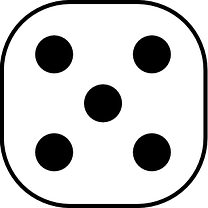
\includegraphics[width=0.1in]{Dice/die5} wins.

\begin{enumerate}
\def\labelenumi{\arabic{enumi}.}
\tightlist
\item
  Find the probability that the first player to throw the die wins.
\item
  Suppose the player who throws first is selected by the toss of a fair coin.
  Show that each player still has an equal chance of winning.
\end{enumerate}

\end{exercise}

\begin{exercise}
\protect\hypertarget{exr:RandomisedResponse}{}\label{exr:RandomisedResponse}

To get honest answers to sensitive questions, sometimes the \emph{randomised response technique} is used.
For example, suppose the aim is to discover the proportion of students who have used illegal drugs in the past week.

\(N\) cards are prepared, where \(m\) have the statement `I \emph{have} used an illegal drug in the past week'.
The remaining \(N - m\) cards have the statement `I \emph{have not} used an illegal drug in the past week'.

Each student in the sample then selects one card at random from the prepared pile of \(N\)~cards, and answers `True' or `False' when asked the question `Is the statement on the selected card true or false?' without divulging which statement is on the card.
Since the interviewer does not know which card has been presented, the interviewer does not know if the person has used drugs or not from this answer.

Let~\(T\) be the probability that a student answers `True', and~\(p\) be the probability that a student chosen at random has used an illegal drug.
Assume that each student answers the question on the chosen card truthfully.

\begin{enumerate}
\def\labelenumi{\arabic{enumi}.}
\tightlist
\item
  From an understanding of the problem, show that
  \[
    T = (1 - p) + \frac{m}{N}(2p - 1).
  \]
\item
  Find an expression for~\(p\) in terms of~\(T\), \(m\) and~\(N\) by rearranging the previous expression.
\item
  Explain what happens for \(m = 0\), \(m = N\) and \(m = N/2\), and why these make sense \emph{in the context of the question}.
\item
  Suppose that, in a sample of 400 students, 175 answer `True'.
  Estimate~\(p\) from the expression found above, given that \(N = 100\) and \(m = 25\).
\end{enumerate}

\end{exercise}

\begin{exercise}
\protect\hypertarget{exr:MCExam}{}\label{exr:MCExam}A multiple choice question contains~\(m\) possible choices.
There is a probability of~\(p\) that a candidate chosen at random will know the correct answer.
If a candidate does \emph{not} know the answer, the candidate guesses and is then equally likely to select any of the~\(m\) choices.

For a randomly selected candidate, what is the probability of the question being answered correctly?
\end{exercise}

\begin{exercise}
\protect\hypertarget{exr:EPL}{}\label{exr:EPL}

In the 2019/2020 English Premier League (EPL), at full-time the home team had won \(91\) out of \(208\) games, the away team won \(67\), and \(50\) games were drawn.
(Data from: \url{https://sports-statistics.com/sports-data/soccer-datasets/})

Define \(W\) as a win, and \(D\) as a draw.

\begin{enumerate}
\def\labelenumi{\arabic{enumi}.}
\tightlist
\item
  Explain the difference between \(\Pr(W)\) and \(\Pr(W \mid D^c)\).
\item
  Compute both probabilities, and comment.
\end{enumerate}

\end{exercise}

\begin{exercise}
\protect\hypertarget{exr:TwoPointsInSquare}{}\label{exr:TwoPointsInSquare}

Consider a square of size \(1\times 1\) metre.
A random process consists of selecting two points at random in the square.

\begin{enumerate}
\def\labelenumi{\arabic{enumi}.}
\tightlist
\item
  What is the sample space for the distance between the two points?
\item
  Suppose a grid (lines parallel to the sides) is drawn on the square such that grid lines are equally spaced \(25\)~cm apart.
  Two points are chosen again, but must be on the intersection of the grid lines.
  Write some \textbf{R} code to generate the sample space for the distance between the two points.
\end{enumerate}

\end{exercise}

\begin{exercise}
\protect\hypertarget{exr:LocalNewsletter}{}\label{exr:LocalNewsletter}

Suppose that \(30\)\% of the residents of a certain suburb subscribe to a local newsletter.
In addition, \(8\)\% of residents belong to a local online group.

\begin{enumerate}
\def\labelenumi{\arabic{enumi}.}
\tightlist
\item
  What percentage of residents \emph{could} belong to both?
  Give a range of possible values.
\item
  Suppose \(6\)\% belong to both.
  Compute:

  \begin{enumerate}
  \def\labelenumii{\alph{enumii}.}
  \tightlist
  \item
    The probability than a random chosen newsletter subscriber is also a member of the online group.
  \item
    The probability than a random chosen online member is also a subscriber to the newsletter.
  \end{enumerate}
\end{enumerate}

\end{exercise}

\begin{exercise}
\protect\hypertarget{exr:SchoolKids}{}\label{exr:SchoolKids}

The data in Table~\ref{tab:EdTable} tabulates information about school children in Queensland in 2019 (\citeproc{ref-mypaper:Dunn:GLM-IEE}{Dunn 2023}).

\begin{enumerate}
\def\labelenumi{\arabic{enumi}.}
\tightlist
\item
  What is the probability that a randomly chosen student is a First Nations student?
\item
  What is the probability that a randomly chosen student is in a government school?
\item
  Is the sex of the student approximately independent of whether the student is a First Nations student, for students in government schools?
\item
  Is the sex of the student approximately independent of whether the student is a First Nations student, for students in non-government schools?
\item
  Is whether the student is a First Nations student approximately independent of the type of school, for female students?
\item
  Is whether the student is a First Nations student approximately independent of the type of school, for male students?
\item
  Based on the above, what can you conclude from the data?
\end{enumerate}

\end{exercise}

\begin{table}
\centering
\caption{\label{tab:EdTable}The number of First Nations and non-First Nations students in Queensland schools in 2019.}
\centering
\fontsize{10}{12}\selectfont
\begin{tabular}[t]{l>{\raggedleft\arraybackslash}p{30mm}>{\raggedleft\arraybackslash}p{30mm}}
\toprule
\textbf{ } & \textbf{Number of First Nations students} & \textbf{Number of non-First Nations students}\\
\midrule
\addlinespace[0.3em]
\multicolumn{3}{l}{\textit{Government schools}}\\
\hspace{1em}Females & 2,540 & 21,219\\
\hspace{1em}Males & 2,734 & 22,574\\
\addlinespace[0.3em]
\multicolumn{3}{l}{\textit{Non-government schools}}\\
\hspace{1em}Females & 391 & 9,496\\
\hspace{1em}Males & 362 & 9,963\\
\bottomrule
\end{tabular}
\end{table}

\begin{exercise}
\protect\hypertarget{exr:CardsAces}{}\label{exr:CardsAces}

Two cards are randomly drawn (without replacement) from a \(52\)-card pack.

\begin{enumerate}
\def\labelenumi{\arabic{enumi}.}
\tightlist
\item
  What is the probability the second card is an \textbf{Ace}?
\item
  What is the probability that the first card is lower in rank (\textbf{Ace} low) than the second?
\item
  What is the probability that the card ranks are in consecutive order where \textbf{Ace} is low \emph{or} high and order is irrelevant (e.g., (Jack, Queen), (Queen, Jack), (Ace, Two) or (King, Ace))?
\end{enumerate}

\end{exercise}

\begin{exercise}
\protect\hypertarget{exr:Octaves}{}\label{exr:Octaves}

An octave contains \(12\) distinct notes: seven white keys and 5 black keys on a piano.

\begin{enumerate}
\def\labelenumi{\arabic{enumi}.}
\tightlist
\item
  How many different eight-note sequences within a single octave can be played using the white keys only?
\item
  How many different eight-note sequences within a single octave can be played if the white and black keys alternate (starting with either colour)?
\item
  How many different eight-note sequences within a single octave can be played if the white and black keys alternate and no key is played more than once?
\end{enumerate}

\end{exercise}

\begin{exercise}
\protect\hypertarget{exr:SomeProb}{}\label{exr:SomeProb}Find \(\Pr(A\cap B)\) if \(\Pr(A) = 0.2\), \(\Pr(B) = 0.4\), and \(\Pr(A\mid B) + \Pr(B \mid A) = 0.375\).
\end{exercise}

\begin{exercise}
\protect\hypertarget{exr:TwoEventsOverline}{}\label{exr:TwoEventsOverline}Suppose the events \(A\) and \(B\) have probabilities \(\Pr(A) = 0.4\) and \(\Pr(B) = 0.3\), and \(\Pr(A\cup B) = 0.5\).
Determine \(\Pr( A^c \cap B^c)\).
Are \(A\) and \(B\) independent events?
\end{exercise}

\begin{exercise}
\protect\hypertarget{exr:SolvePermk}{}\label{exr:SolvePermk}

Solve \(12\times P^7_k = 7\times P^6_{k + 1}\) using:

\begin{enumerate}
\def\labelenumi{\arabic{enumi}.}
\tightlist
\item
  algebra; and then
\item
  using \textbf{R} to search over all possible values of \(k\).
\end{enumerate}

\end{exercise}

\begin{exercise}
\protect\hypertarget{exr:SolvePermk2}{}\label{exr:SolvePermk2}Solve \(P^7_{r + 1} = 10 {C^7_r}\) for \(r\).
\end{exercise}

\begin{exercise}
\protect\hypertarget{exr:BirthdayProblem}{}\label{exr:BirthdayProblem}

Take a guess: how many randomly-selected individuals would you need so that the probability that \emph{at least two} have the same birthday would exceed~\(50\)\%?

\begin{enumerate}
\def\labelenumi{\arabic{enumi}.}
\tightlist
\item
  Show that the probability that, for a group of \(N\)~randomly selected individuals, \emph{at least two} have the same birthday (assuming~\(365\) days in a year) can be written as
  \[
    1 - \left(\frac{365}{365}\right) \times \left(\frac{364}{365}\right) \times \left(\frac{363}{365}\right) \times \dots\times \left(\frac{365 - n + 1}{365}\right).
  \]
\item
  Graph the relationship for various values of~\(N\), using the above form to compute the probability.
\item
  What assumptions are necessary?
  Are these reasonable?
\item
  Use computer simulation to confirm these results.
\end{enumerate}

\end{exercise}

\begin{exercise}
\protect\hypertarget{exr:SixNumbersConsecutive}{}\label{exr:SixNumbersConsecutive}Six numbers are randomly selected \emph{without replacement} from the numbers \(1, 2, 3,\dots, 45\).
Model this process using \textbf{R} to estimate the probability that there are \emph{no consecutive numbers} amongst the numbers selected.
(That is, no sequence like \texttt{4,\ 5} or \texttt{33,\ 34} or \texttt{21,\ 22,\ 23} appears, once the numbers are sorted smallest to largest.)
\end{exercise}

\begin{exercise}
\protect\hypertarget{exr:NewCars}{}\label{exr:NewCars}A new cars can be purchased with options:

\begin{itemize}
\tightlist
\item
  Seven different paints colours are available;
\item
  Three different trim levels are available;
\item
  Cars can be purchased with or without a sunroof.
\end{itemize}

How many possible combinations are possible?
\end{exercise}

\begin{exercise}
\protect\hypertarget{exr:NumberPlates}{}\label{exr:NumberPlates}Suppose number plates have three numbers, followed by two letters then another number.
How many number plates are possible with this scheme?
\end{exercise}

\begin{exercise}
\protect\hypertarget{exr:PairsPoker}{}\label{exr:PairsPoker}

In some forms of poker, five cards are dealt to each player, and certain combinations then beat other combinations.

\begin{enumerate}
\def\labelenumi{\arabic{enumi}.}
\tightlist
\item
  What is the probability that the initial five cards include \emph{exactly} one pair.
  (This implies \emph{not} getting a three of a kind or four of a kind.)
  Explain your reasoning.
\item
  What is the probability that the initial five cards includes \emph{only} picture cards (Ace, King, Queen, Jack)?
\end{enumerate}

\end{exercise}

\begin{exercise}
Prove that \(P^n_n = P^n_{n-1}\).
\end{exercise}

\begin{exercise}
\protect\hypertarget{exr:NoTechP}{}\label{exr:NoTechP}Without using any technology, compute the value of \(\displaystyle \frac{C^{25}_8}{C^{25}_6}\).
\end{exercise}

\begin{exercise}
\protect\hypertarget{exr:ProbHarder}{}\label{exr:ProbHarder}\leavevmode

\begin{enumerate}
\def\labelenumi{\arabic{enumi}.}
\tightlist
\item
  If \(A_1, A_2, \dots, A_n\) are independent events, prove that
  \[
  \Pr(A_1 \cup A_2 \cup \dots \cup A_n) = 1 - [1 - \Pr(A_1)][1 - \Pr(A_2)] \dots [1 - \Pr(A_n)].
  \]
\item
  Consider two events \(A\) and \(B\) such that \(\Pr(A) = r\) and \(\Pr(B) = s\) with \(r, s > 0\) and \(r + s > 1\).
  Prove that
  \[
     \Pr(A \mid B) \ge 1 - \left(\frac{1 - r}{s} \right).
  \]
\end{enumerate}

\end{exercise}

\begin{exercise}
\protect\hypertarget{exr:AngleInSquare}{}\label{exr:AngleInSquare}Consider the diagram in Fig.~\ref{fig:AngleInSquare}.
The point \(P\) is randomly placed within the \(1\times 1\) square \(ABCD\).
What is the probability that the angle \(APB\) is \emph{greater} than \(90^\circ\)?
\end{exercise}

\begin{figure}

{\centering 
\includegraphics[width=0.3\linewidth]{03-Probability_files/figure-latex/AngleInSquare-1} 

}

\caption{Point $P$ is placed randomly in the $1\times 1$ square $ABCD$.}\label{fig:AngleInSquare}
\end{figure}

\begin{exercise}
\protect\hypertarget{exr:SquareInCircle}{}\label{exr:SquareInCircle}Consider the diagram in Fig.~\ref{fig:SquareInCircle}.
What is the probability that a point randomly placed within the circle (with radius \(r = 1\)) also lands within the square?
\end{exercise}

\begin{figure}

{\centering 
\includegraphics[width=0.3\linewidth]{03-Probability_files/figure-latex/SquareInCircle-1} 

}

\caption{A random point is placed within the circle with centre\ $C$ and radius $r = 1$.}\label{fig:SquareInCircle}
\end{figure}

\begin{exercise}
\protect\hypertarget{exr:Locks}{}\label{exr:Locks}A combination lock work by setting (for example) four digits to numbers in a specified order.
Suggest a more accurate name for a `\emph{combination} lock'.
\end{exercise}

\begin{exercise}
\protect\hypertarget{exr:NonTransitiveDice}{}\label{exr:NonTransitiveDice}Consider the following dice (called Miwin's dice)\index{Miwin's dice};:

\begin{itemize}
\tightlist
\item
  Die~A: The six sides are labelled: \(\qquad  2 \qquad 2 \qquad 4 \qquad 4 \qquad 9 \qquad 9\).
\item
  Die~B: The six sides are labelled: \(\qquad  1 \qquad 1 \qquad 6 \qquad 6 \qquad 8 \qquad 8\).
\item
  Die~C: The six sides are labelled: \(\qquad  3 \qquad 3 \qquad 5 \qquad 5 \qquad 7 \qquad 7\).
\end{itemize}

These dice are \emph{non-transitive} that is, in the long run, Die~A beats Die~B, Die~B beats Die~C\ldots{} but Die~C also beats Die~A.

Use a computer simulation to confirm these results by `rolling' them many times, and find the probabilities of each die winning against the other two.
\end{exercise}

\begin{exercise}
\protect\hypertarget{exr:SimulationSensivityNumber}{}\label{exr:SimulationSensivityNumber}Adjust the \textbf{R} code used in Sect.~\ref{SimulationSensitivityAnalysis} so examine how the probability of running late changes as the number of booked patients increases from \(15\)~up to \(25\) people.
\end{exercise}

\begin{exercise}
\protect\hypertarget{exr:SimulationMontyHall}{}\label{exr:SimulationMontyHall}

A game show contestant is told there is a car behind one of three doors, and a goat behind each of the other doors.
The contestant is asked to select a door.

The host of the show (who knows where the car is) now opens one of the doors \emph{not} selected by the contestant, and reveals a goat.
The host now gives the contestant the choice of either (a)~retaining the door chosen first, or (b)~switching and choosing the other (unopened) door.

\begin{enumerate}
\def\labelenumi{\arabic{enumi}.}
\tightlist
\item
  Which of the following \emph{do you think} is the contestant's best strategy?
\item
  Always retain the first choice.
\item
  Always change and select the other door.
\item
  Choose either unopened door at random.
\item
  Use a computer simulation to estimate the probabilities to determine the best strategy.
  \emph{Hint:} remember the crucial information: the host of the show knows where the car is, and opens one of the doors \emph{not} selected by the contestant, \emph{and reveals a goat}.
\end{enumerate}

\end{exercise}

\begin{exercise}
\protect\hypertarget{exr:SimulationRunningLate}{}\label{exr:SimulationRunningLate}

Suppose a specialist doctors surgery schedules a maximum of~\(20\) patients per day, but history shows that each patient has a chance of not showing up (a `no-show').
For simplicity, assume that each patient has the same `no-show' probability, and that patients operate independently.
If more than~\(15\) patients show up on any one day, the clinic runs late by the end of the day.

\begin{enumerate}
\def\labelenumi{\arabic{enumi}.}
\tightlist
\item
  What is the probability the clinic runs late?
  Write an \textbf{R} function that allows for a simulation to answer the question.
\item
  Perform a sensitivity analysis, where the probability that each patients is a no-show varies (e.g., \(10\)\%; \(15\)\%; \(20\)\%), to see the impact this has on the probability that the clinic runs late.
\item
  Perform a sensitivity analysis to see the impact on the probability of running late, if between~\(18\) and~\(25\) patients are booked per day.
\end{enumerate}

\end{exercise}

\begin{exercise}
\protect\hypertarget{exr:SimulationCards}{}\label{exr:SimulationCards}Consider drawing five cards at random from a fair pack; what is the probability that at least cards~\(3\) are hearts?

This question is not too difficult to answer using the counting methods of Sect.~\ref{CombsAndPerms}; you should show that the answer is approximately~\(0.0927\) using these methods.

Create an \textbf{R} simulation to check the answer.
\end{exercise}

\chapter{Random variables and their distributions}\label{DistributionRandomVariables}

\begin{objectivesBox}{iconmonstr-target-4-240.png}

Upon completion of this chapter, you should be able to:

\begin{itemize}
\tightlist
\item
  distinguish between discrete, continuous and mixed random variables.
\item
  determine the probability function of random variables defined for a random process.
\item
  determine the distribution function of a random variable from its probability function.
\item
  apply probability functions and distribution functions to compute probabilities for defined events.
\item
  plot the probability function and distribution function of a random variable.
\end{itemize}

\end{objectivesBox}

\section{Random variables}\label{RandomVariables}

Chapter~\ref{ChapterProbability} introduced the language and tools of probability to describe uncertainty.
The concept of the \hyperref[def:SampleSpace]{\emph{sample space}} was introduced, which describes the possible outcomes of a \hyperref[def:RandomProcess]{\emph{random process}}.
Often, however, the individual elements of the sample space are not directly of interest, especially if the sample space is large or infinite.
Subsets of these sample space elements are usually of greater interest and more convenient to work with.

For example, the sample space for observing the rolls of two dice (Example~\ref{exm:TwoDice}) contains~\(36\) elements.
We may be interested in the \emph{sum} of the two rolls, rather than which elements in the sample space produce a given sum.
That is, we may be more interested in \emph{whether} we roll a sum of~\(5\) than \emph{which} elements of the sample space give rise to a sum of~\(5\).
Outcomes that share a common numerical property are often grouped together.

Rather than working directly with outcomes, we often map outcomes to numbers that represent quantities of interest.
This leads to the idea of a \emph{random variable}.
\emph{Random variable} is sometimes abbreviated to \emph{rv} or \emph{RV}.
In probability theory, a random variable is a function from the sample space to the real numbers that encodes outcomes numerically.

\begin{definition}[Random variable]
\protect\hypertarget{def:RandomVariable}{}\label{def:RandomVariable}A \emph{random variable}\index{Random variable} is a function that assigns a real number to each outcome~\(s\) in the sample space~\(S\).
A random variable~\(X\) maps \(S\to\mathbb{R}\), and the value assigned to an outcome \(s\in S\) is written~\(X(s)\).
\end{definition}

A random variable is a deterministic function evaluated at a random outcome.
The function~\(X\) is deterministic; the randomness arises from the random outcome~\(s\) to which it is applied.

\begin{importantBox}{iconmonstr-warning-8-240.png}
Formally, a random variable is a \emph{measurable} function.
This condition ensures that probabilities such as \(\Pr(X\le x)\) are well-defined.
In this book, all random variables considered satisfy this condition.

\end{importantBox}

Many random variables take only integer values, such as the number of heads in three coin tosses; these are called \emph{discrete} random variables.
Many random variables take values in an interval, such as the height of a randomly chosen person; these are \emph{continuous} random variables.
\emph{Mixed} random variables have both discrete probability mass and a continuous density component.
In all cases, \(X(s)\) is a real number, but the set of possible values of \(X\) may be a finite set, a countable set (like the integers), or an interval in \(\mathbb{R}\).

\begin{importantBox}{iconmonstr-warning-8-240.png}
\emph{Random variables} are different from \emph{variables} used in algebra.
In algebra, a variable typically represents an unknown but fixed quantity.
In contrast, a random variable represents a quantity whose value depends on the outcome of a random process.

\end{importantBox}

\begin{definition}[Domain and range]
\protect\hypertarget{def:DomainRange}{}\label{def:DomainRange}The \emph{domain}\index{Domain} of a random variable is the sample space~\(S\), and the \emph{range}\index{Range} (or \emph{support},\index{Support} or \emph{value set})\index{Value set} is the set of real numbers taken by a function.

The \emph{range} for a random variable~\(X\) is often denoted~\(\mathcal{R}_X\), where \(\mathcal{R}_X\subseteq\mathbb{R}\).
The domain of~\(X\) is the set~\(S\), and the range is the set \(\{X(s)\mid s\in S\}\).
\end{definition}

Since \(X\) is a function, each \(s\in S\) is assigned to exactly one value \(X(s)\); however, multiple values of \(s\in S\) may be assigned to the same value of \(X(s)\).
The variable is \emph{random} since its value depends upon the outcome of the random process.

A capital letter (such as \(X\) or \(Y\)) is usually used to denote the \emph{description} of the random variable, while lower-case letters (such as \(x\) or \(y\)) are used to represent a realised value.
For example, consider rolling two dice and observing the sum of the two rolls.
Writing \(X = 3\) means:

\begin{itemize}
\tightlist
\item
  `The random variable~\(X\)' (e.g., the description `the sum of the roll of two dice')\ldots{}
\item
  `\ldots{} was observed to take the value~\(3\) in some outcome of the random process'.
\end{itemize}

Sometimes, \(X\) is written for both the function and its value; the meaning is usually clear from context.

\begin{example}[Rolling a die twice]
\protect\hypertarget{exm:TossDieTwiceProduct}{}\label{exm:TossDieTwiceProduct}Consider rolling a fair die twice.
The sample space~\(S\) contains \(36\)~elements shown in Table~\ref{tab:TwoDice}:
\[
  S = \{ (1, 1), (1, 2), (1, 3), \dots (6, 5), (6, 6)\}.
\]
However, we may be interested in the random variable~\(X\), the \emph{product} of the two numbers rolled.
Each element~\(s_i\) of~\(S\) can be assigned to exactly one real number (in this case, to exactly one \emph{integer}):
\begin{align*}
  (1, 1) &\mapsto X = 1;\\
  (1, 2) &\mapsto X = 2;\\
  (1, 3) &\mapsto X = 3;\\
  \vdots &\qquad   \vdots\\
  (6, 5) &\mapsto X = 30;\\
  (6, 6) &\mapsto X = 36.
\end{align*}
Each element of the sample space is mapped to exactly one value of~\(X\).
However, multiple elements of the sample space can be mapped to the same value of~\(X\):
\begin{align*}
 (3, 4) &\mapsto X = 12; \quad\text{and}\\
 (6, 2) &\mapsto X = 12; \quad\text{and}\\
 (2, 6) &\mapsto X = 12.
\end{align*}
Writing \(X = 12\) means `the product of the numbers on the two rolls is~\(12\)'.
\end{example}

Once a random variable has been defined, events\index{Events} can be defined in terms of the values of the random variable.
Random variables provide a convenient way to express events numerically; rather than listing specific \emph{outcomes}, events can be described using inequalities or equations involving the random variable.

\begin{example}[Rolling a die twice: range]
\protect\hypertarget{exm:TossDieTwiceProductRange}{}\label{exm:TossDieTwiceProductRange}In Example~\ref{exm:TossDieTwiceProduct}, the range of the random variable~\(X\) is
\[
   \mathcal{R}_X = \{1,  2,  3,  4,  5,  6,  8,  9, 10, 12, 15, 16, 18, 20, 24, 25, 30, 36\}.
\]
The domain is the sample space, the set of all ordered pairs
\begin{align*}
  S
  &= \{ (1, 1), (1, 2), (1, 3), \dots (3, 2), (3, 3), (3, 4),\dots (6, 5), (6, 6)\}
  &= \{(r_1, r_2): r_1, r_2\in\{1, \dots, 6\}\}.
\end{align*}
\end{example}

\begin{example}[Rolling a die twice: events]
\protect\hypertarget{exm:TossDieTwiceProductEvents}{}\label{exm:TossDieTwiceProductEvents}The random variable~\(X\) in Example~\ref{exm:TossDieTwiceProduct} can be used to define different events.
For example, we could define Event~\(A_1\) as
\[
  \{s \in S \mid  X(s) > 10\},
\]
usually written more succinctly as \(X > 10\).
Other events can be defined also:
\begin{align*}
   A_2 &= \{\text{$4 \le X < 10$}\} = \{ 4,  5,  6, 8,  9 \};\\
   A_3 &= \{\text{$X < 0$ }\} = \varnothing;\\
   A_4 &= \{\text{$X$ is prime}\} = \{2, 3, 5 \};\\
   A_5 &= \{\text{$X$ is evenly divisible by\ $8$}\} = \{ 8, 16, 24\}.
\end{align*}
\end{example}

\begin{example}[Sum of two die rolls]
\protect\hypertarget{exm:TwoDiceRV}{}\label{exm:TwoDiceRV}Consider observing the rolls of two dice.
The sample space contains~\(36\) elements (Example~\ref{exm:TwoDice}), and can be denoted using the ordered pairs \((r_1, r_2)\), where \(r_1\) and \(r_2\) are the results of die~\(1\) and~\(2\) respectively.
The sample space is listed in Table~\ref{tab:TwoDice}.
For example, we could define \(s_1\) as the sample point \((1, 1)\).

The random variable~\(Y\) can be defined on this sample space as:
\[
   Y(s)  = \text{the sum of the two rolls in $s$} = r_1 + r_2.
\]
This definition assigns a real number to each outcome in the sample space:

\begin{longtable}[]{@{}lc@{}}
\toprule\noalign{}
\textbf{Sample space elements} & \textbf{Value of random variable \(Y\)} \\
\midrule\noalign{}
\endhead
\bottomrule\noalign{}
\endlastfoot
(1, 1) & 2 \\
(1, 2), (2, 1) & 3 \\
(1, 3), (2, 2), (3, 1) & 4 \\
\(\vdots\) & \(\vdots\) \\
(6, 6) & 12 \\
\end{longtable}

For example, the elements of~\(S\) assigned to \(Y = 4\) are
\[
   (1, 3), (2, 2)\quad\text{and}\quad (3, 1).
\]
Notice that many elements of the sample space can be assigned to the same value of the random variable (which is typical for random variables).

The \emph{domain} of~\(Y\) is the sample space~\(S\); the \emph{range} is
\[
   \mathcal{R}_Y = \{ Y(s) \mid s\in S\} = \{2, 3, \dots, 12\}.
\]
\end{example}

\begin{example}[Tossing a coin till a head appears]
\protect\hypertarget{exm:TossCoinTillHead}{}\label{exm:TossCoinTillHead}Consider the random process `tossing a coin until a Head is observed'.
The sample space is
\[
   \Omega = \{H, TH, TTH, TTTH, \dots \}.
\]
We could then define the random variable \(N\) as `the number of tosses until the first head is observed'.
\(\Omega\) is countably infinite.
Then each element of the sample space is assigned to a positive integer:
\begin{align*}
   H\quad    &\text{is assigned to $N = 1$};\\
   TH\quad   &\text{is assigned to $N = 2$};\\
   TTH\quad  &\text{is assigned to $N = 3$};\\
   \vdots\quad &\qquad \vdots
\end{align*}
and so on.
Writing \(N = 2\) means `the number of tosses to observe the first head is two'.
\end{example}

\begin{example}[Drawing two cards]
\protect\hypertarget{exm:DrawTwoCards}{}\label{exm:DrawTwoCards}Consider drawing two cards from a standard, well-shuffled pack of cards, and observing the colour of the card (B: Black; R: Red).
The sample space~\(\Omega\) is:
\[
   \Omega = \{ BB, BR, RR, RB\}.
\]
Many random variables could be defined on this sample space; for example:
\begin{align*}
   T&: \text{The number of black cards drawn};\\
   M&: \text{The number of red cards drawn};\\
   D&: \text{The number of black cards drawn,}\\
    &\quad \text{minus the number of red cards drawn}.
\end{align*}
All of these assign a real number to each element of~\(\Omega\).
The random variable~\(D\), for instance, is defined as:

\begin{longtable}[]{@{}ll@{}}
\toprule\noalign{}
\textbf{Sample space elements} & \textbf{Value of \(D\)} \\
\midrule\noalign{}
\endhead
\bottomrule\noalign{}
\endlastfoot
\(BR\) and \(RB\) & \(D = 0\) \\
\(BB\) & \(D = 2\) \\
\(RR\) & \(D = -2\) \\
\end{longtable}

The domain is \(\Omega\), and the range is
\[
   \mathcal{R}_D = \{ D(s) \mid s\in \Omega\} = \{-2, 0, 2\}.
\]
\end{example}

\section{Discrete, continuous and mixed random variables}\label{DiscreteContMixed}

As observed earlier, random variables can be discrete, continuous, or mixed.
Each are discussed in the sections that follow.

\subsection{Discrete random variables}\label{RVsDiscrete}

\begin{definition}[Discrete random variable]
\protect\hypertarget{def:DiscreteRV}{}\label{def:DiscreteRV}A \textbf{discrete random variable} takes values in a finite or countable infinite set.
Its distribution is described using a probability mass function.
\end{definition}

\begin{example}
In Example~\ref{exm:TossDieTwiceProduct}, exactly~\(36\) values of the random variable~\(X\) are possible: \(1, 2, \dots 36\).

In Example~\ref{exm:TwoDiceRV}, exactly~\(11\) values of the random variable~\(Y\) are possible: \(2, 3, \dots 12\).

In Example~\ref{exm:TossCoinTillHead}, the random variable~\(N\) takes a \emph{countably infinite} number of possible values: \(1, 2, 3, \dots\)

In Example~\ref{exm:DrawTwoCards}, the random variable~\(D\) can take one of three possible values: \(-2\), \(0\) or \(2\).

These are all \emph{discrete} random variables.
\end{example}

The definition refers to the values of random variable, not to the \hyperref[def:SampleSpace]{sample space}.
Examples of discrete random variables include:

\begin{itemize}
\tightlist
\item
  The number of children aged under~\(18\) living in a household.
\item
  The number of errors per month.
\item
  The number of incidents of lung cancer at a hospital in the last \(28\)~days.
\item
  The number of cyclones per season.
\item
  The number of wins by a football team.
\item
  The number of kangaroos observed in a five-hectare transect.
\end{itemize}

\subsection{Continuous random variables}\label{RVsContinuous}

For a continuous sample space, the random variable is usually the \emph{identity function} \(Y(s) = s\).
For example, in Example~\ref{exm:CricketBallDefine} the sample space that describes how far a cricket ball can be thrown is already defined on the positive reals.
Hence, we can define the random variable as \(T(s) = s\), where~\(s\) is the distance specified in the sample space.

\begin{definition}[Continuous random variable]
\protect\hypertarget{def:ContinuousRF}{}\label{def:ContinuousRF}A \textbf{continuous random variable} can take values in a continuum (an uncountable set of values), and \(\Pr(X = x) = 0\) for all~\(x\).
Its distribution is described using a probability density function.
\end{definition}

A continuous random variable is one that can take values on a continuous scale (such as all real numbers in an interval), rather than only distinct separate values.
The value of a continuous random variable can never, in principle, be measured exactly, so in practice needs to be rounded.

\begin{example}[Heights]
\protect\hypertarget{exm:ContinuousRVHeight}{}\label{exm:ContinuousRVHeight}Height \(H\) is often recorded to the nearest centimetre (e.g., \(179\,\text{cm}\)) for convenience and practicality.
Better measuring instruments may be able to record height to one or more decimal places of a centimetre.
The range is \(\mathcal{R}_H = \{ H(s) \mid s \in (0, \infty)\}\), or \(\mathcal{R}_H = \{ H(s) \mid s \in \mathbb{R}_{+}\}\).
\end{example}

\begin{importantBox}{iconmonstr-warning-8-240.png}
Even though \emph{your} height may not change, the notion of a \emph{random variable} means that height varies from one realisation of the random process to another; that is, from one \emph{person} to the next.

\end{importantBox}

Examples of continuous random variables include:

\begin{itemize}
\tightlist
\item
  The volume of waste water treated at a sewage plant per day.
\item
  The weight of hearts in rats.
\item
  The lengths of the wings of butterflies.
\item
  The yield of barley from a large paddock.
\item
  The amount of rainfall recorded each year.
\item
  The time taken to perform a psychological test.
\item
  The percentage cloud cover.
\end{itemize}

\subsection{Mixed random variables}\label{RVsMixed}

Some random variables are not completely discrete or continuous; these are called \emph{mixed random variables}.
A common example in applications is a random variable that is continuous on the positive real numbers, with a discrete probability mass at zero.

\begin{definition}[Mixed random variable]
\protect\hypertarget{def:MixedRV}{}\label{def:MixedRV}A \textbf{mixed random variable} has a distribution with both discrete probability mass and a continuous density component.
\end{definition}

A mixed random variable has some values with positive probability and also a continuous range of possible values described by a density function.
In this book, we only consider mixed random variables with a point mass at \(X = 0\) and a continuous component on~\(\mathbb{R}_{+}\), although more general mixtures are possible.

\begin{example}[Vehicle wait times]
\protect\hypertarget{exm:MixedVehicleWait}{}\label{exm:MixedVehicleWait}Consider the time spent by vehicles waiting at a set of traffic lights before proceeding through the intersection.

If the light is green on arrival, the wait time is zero: the vehicle proceeds immediately.
Thus, there is a positive probability that the waiting time is exactly zero.
If the light is red on arrival, the vehicle waits a continuously varying amount of time until the light turns green.

The waiting time is therefore a \emph{mixed random variable}, with a discrete probability mass at zero and a continuous distribution for positive waiting times.
\end{example}

Examples of mixed random variables include:

\begin{itemize}
\tightlist
\item
  The amount of rainfall that falls in a month (zero, or a continuous amount).
\item
  The weight of fruit produced per tree (zero if no fruit is produced, or a continuous amount).
\item
  The mass of fish-catch per trawl (zero if no fish are caught, or a continuous amount).
\item
  Insurance claim size (zero if no claim, or a continuous positive amount otherwise)
\item
  Purchase amount in a store (zero if no purchase, positive continuous amount otherwise)
\end{itemize}

\section{Probability functions}\label{UnivariateProbabilityFunctions}

The previous section introduced \emph{random variables}: real values assigned to outcomes in the sample space.
Often, many elements of the sample space were assigned to the same value of the random variable.
Therefore, \emph{probabilities} can be assigned to various values of the random variable, to develop a \emph{probability model} for the random variable.

A \emph{model} describes theoretical patterns over infinite trials.
On any single roll of a die, a
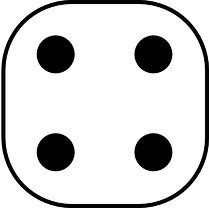
\includegraphics[width=0.1in]{Dice/die4} may or may not occur, but theoretically (and for infinite rolls) we expect a
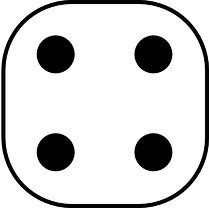
\includegraphics[width=0.1in]{Dice/die4} to appear~\(1/6\) of the time.
A \emph{probability model} describes the probability that various values of the random variable might appear on any one realisation in theory.

This probability model is called the \emph{probability function}.

\begin{example}[Tossing coin outcomes]
\protect\hypertarget{exm:TossingCoinOutcomes}{}\label{exm:TossingCoinOutcomes}Consider tossing a coin twice and observing the outcome of the two tosses.
Since a random variable is a \emph{real-valued function}, simply observing the outcome as \((H, T)\), for example, does not define a random variable.

We could define the random variable of interest, say~\(H\), as the \emph{number} of heads on the two tosses of the coin.
The \emph{sample space} for the experiment is
\[
   S = \{ TT, TH, HT, HH\}.
\]
The connection between the sample space and~\(H\) is shown in the table below.
In this case, the range of \(H\) is \(\mathcal{R}_H = \{0, 1, 2\}\).
The probability of observing each value of~\(H\) can be computed using classical probability:

\begin{longtable}[]{@{}
  >{\centering\arraybackslash}p{(\linewidth - 6\tabcolsep) * \real{0.1828}}
  >{\centering\arraybackslash}p{(\linewidth - 6\tabcolsep) * \real{0.4194}}
  >{\centering\arraybackslash}p{(\linewidth - 6\tabcolsep) * \real{0.1935}}
  >{\centering\arraybackslash}p{(\linewidth - 6\tabcolsep) * \real{0.2043}}@{}}
\toprule\noalign{}
\begin{minipage}[b]{\linewidth}\centering
\emph{Element of \(S\)}
\end{minipage} & \begin{minipage}[b]{\linewidth}\centering
\emph{Function \(H(s)\)}
\end{minipage} & \begin{minipage}[b]{\linewidth}\centering
\emph{Value of \(H\)}
\end{minipage} & \begin{minipage}[b]{\linewidth}\centering
\emph{\(\Pr(s_i)\)}
\end{minipage} \\
\midrule\noalign{}
\endhead
\bottomrule\noalign{}
\endlastfoot
\(s_1 = TT\) & \(H(s_1)\): Number of heads in \(s_1\) & 0 & \(1/4\) \\
\(s_2 = TH\) & \(H(s_2)\): Number of heads in \(s_2\) & 1 & \(1/4\) \\
\(s_3 = HT\) & \(H(s_3)\): Number of heads in \(s_3\) & 1 & \(1/4\) \\
\(s_4 = HH\) & \(H(s_4)\): Number of heads in \(s_4\) & 2 & \(1/4\) \\
\end{longtable}

The \emph{probability function} could be defined as
\begin{align*}
      \Pr(H = 0):&\quad 1/4\\
      \Pr(H = 1):&\quad 1/2\\
      \Pr(H = 2):&\quad 1/4\\
      \Pr(H = h):&\quad 0\quad \text{for all other values of $h$}.
\end{align*}
\end{example}

Probability functions are written and interpreted differently, depending on whether the random variable is a discrete, continuous or mixed random variable.

\subsection{Discrete random variables: probability mass functions}\label{ProbabilityFunctionsDiscrete}

For a discrete random variable, the probability function indicates how probabilities are assigned to the values of the discrete random variable.
For a discrete random variable, the probability function is often called the \emph{probability mass function} (or PMF).

\begin{definition}[Probability function]
\protect\hypertarget{def:ProbabilityFunction}{}\label{def:ProbabilityFunction}Let the range of the discrete random variable~\(X\) be~\(\mathcal{R}_X\).
With each \(x\in \mathcal{R}_X\), associate a number
\[
   p_X(x) = \Pr(X = x).
\]
The function \(p_X(x)\) is called the \emph{probability mass function} of~\(X\).
\end{definition}

The following properties of the probability function are implied by the definition and the rules of probability.

\begin{enumerate}
\def\labelenumi{\arabic{enumi}.}
\tightlist
\item
  \(p_X(t) \ge 0\) for all values of~\(t\); that is, probabilities are never negative.
\item
  \(\displaystyle \sum_{t \in \mathcal{R}_X}  p_X(t) = 1\) where~\(\mathcal{R}_X\) is the range of~\(X\); that is, the probability function covers the probability over all possible sample points in the sample space.
\item
  \(p_X(t) = 0\) if~\(t \notin \mathcal{R}_X\).
\item
  For an event~\(A\subseteq\mathcal{R}_X\) defined on a sample space~\(S\), the probability of event~\(A\) is
  \[
     \Pr(A) = \sum_{t\in A} p_X(t).
  \]
\end{enumerate}

\begin{definition}[Probability distribution]
\protect\hypertarget{def:ProbabilityDistribution}{}\label{def:ProbabilityDistribution}If \(\mathcal{R}_X =\{ x_1, x_2, \dots \}\),
the pair
\[
   \{ \big(x_i, p_X(x_i)\big); \quad i = 1, 2,\dots\}
\]
is called the \emph{probability distribution} of the discrete random variable \(X\).
\end{definition}

The probability distribution of a discrete random variable \(X\) can be represented by listing each outcome with its probability; giving a formula; using a table; or using a graph which displays the probabilities~\(p(x)\) corresponding to each \(x\in \mathcal{R}_X\).

Sometimes the probability function is denoted~\(p(x)\) rather than~\(p_X(x)\).
Using the subscript avoids confusion in situations where many random variables are considered at once.
The subscript is used throughout this book.

The probability distribution of a random variable is a description of the range of the variable and the associated assignment of probabilities.

\begin{example}[Independence]
\protect\hypertarget{exm:Independence}{}\label{exm:Independence}Five balls numbered~\(1\), \(2\), \(3\), \(4\) and~\(5\) are in an urn.
Two balls are selected at random \emph{without} replacement.
Consider finding the probability distribution of the \emph{larger} of the two numbers.
When finding the arger of two numbers, the order is not imoportant, so combinations\index{Combinations} are appropriate, and the number if possible outcomes is therefore
\[
  \binom{5}{2} = 10.
\]
These are easily listed: the sample space is:
\[
    S =\{ (1, 2), (1, 3), (1, 4), (1, 5), (2, 3), (2, 4), (2, 5), (3, 4), (3, 5), (4, 5)\},
\]
where all \(10\)~elements are equally likely.
Then, let~\(X\) be the random variable `the \emph{larger} of the two numbers chosen', so that \(\mathcal{R}_X = \{2, 3, 4, 5\}\).
Listing the probabilities:
\begin{alignat*}{3}
    \Pr(X = 2) &= \Pr\big((1, 2)\big)                                     &\quad &= 1/10;\\
    \Pr(X = 3) &= \Pr\big((1, 3) \text{ or } (2, 3)\big)                 &\quad &= 2/10;\\
    \Pr(X = 4) &= \Pr\big((1, 4) \text{ or } (2, 4) \text{ or } (3, 4)\big) &\quad &= 3/10;\\
    \Pr(X = 5) &= \Pr\big((1, 5) \text{ or } (2, 5) \text{ or } (3, 5)\text{ or } (4, 5)\big) &\quad &= 4/10;\\
    \Pr(\text{other values of } X) & \text{ }                             &\quad &= 0.
\end{alignat*}
This is the probability distribution of~\(X\), which could also be given in a table (Table~\ref{tab:LargestDie}), a graph (Fig.~\ref{fig:ProbDist1}), or as a formula:
\[
   \Pr(X = x) = 
   \begin{cases}
      (x - 1)/10 & \text{for $x = 2, 3, 4, 5$}\\
      0 & \text{elsewhere}.
  \end{cases}
\]
The probability is assumed to be zero for all values not shown.
\end{example}

\begin{table}
\centering
\caption{\label{tab:LargestDie}A table showing the distribution of $X$, the largest number in two draws from an urn.}
\centering
\fontsize{10}{12}\selectfont
\begin{tabular}[t]{lrrrr}
\toprule
$x$ & 2 & 3 & 4 & 5\\
$\Pr(X = x)$ & 0.1 & 0.2 & 0.3 & 0.4\\
\bottomrule
\end{tabular}
\end{table}

\begin{figure}[htbp]
  \centering

  \begin{minipage}{0.9\linewidth}
    \begin{lstlisting}[language=R]


plot( x = 1:6,                           # The values for which PMF > 0
      y = c(0, 0.1, 0.2, 0.3, 0.4, 0),   # The values of f(y)
      xlim = c(0.5, 6.6), ylim = c(0, 0.45),
      type = "h",             # type = "h": vertical lines
      lty = 3,                # lty = 3: Dotted lines 
      las = 1,                # las = 1: Axis labels horizontal 
      col = "grey",           # Use the colour grey
      main = expression(      # Using expression() is slight fancy...
        paste( "The probability distribution of ", italic(X)) 
        ),
      xlab = expression( 
        paste("Values of the random variable ", italic(X)) 
        ),
      ylab = expression( 
        paste( "Probability function ", italic(p)[italic(X)](italic(x)) )
      )
)
points( x = 1:6,  ### Adds the points on top of the vertical lines
        y = c(0, 0.1, 0.2, 0.3, 0.4, 0),
        pch = 19)
    \end{lstlisting}
  \end{minipage}

  \includegraphics[width=0.7\linewidth]{04-RandomVariables_files/figure-latex/LargerTwoNumbers-1.pdf}
  \vspace{0.5em} % Small vertical space between plot and code
  \caption{The probability function for the larger of two numbers drawn.}
  \label{fig:ProbDist1} 
\end{figure}

\begin{example}[Tossing heads]
\protect\hypertarget{exm:TossingHeads}{}\label{exm:TossingHeads}Suppose a fair coin is tossed twice and the uppermost face is noted, as in Example~\ref{TossingCoinOutcomes}.

The probability function is
\[
   p_H(h) = \Pr(H = h) 
          = \begin{cases}
               0.25 & \text{if $h = 0$};\\
               0.5 & \text{if $h = 1$};\\
               0.25 & \text{if $h = 2$};\\
               0 & \text{otherwise}.
              \end{cases}
\]
More succinctly,
\[
   p_H(h) = \Pr(H = h) 
          = \begin{cases}
                  (0.5)0.5^{|h - 1|} & \text{for $h = 0$, $1$ or $2$};\\
                  0 & \text{otherwise}.
              \end{cases}
\]
This information can also be presented as a table (Table~\ref{tab:TwoDieRV}) or graph (Fig.~\ref{fig:ProbDistributionCoin}).
Note that \(\sum_{t \in \{0, 1, 2\}} p_H(t) = 1\) and \(p_H(h)\ge0\) for all \(h\), as required of a pf.
\end{example}

\begin{table}
\centering
\caption{\label{tab:TwoDieRV}A table showing the distribution of $H$, the number of heads in two tosses of a coin.}
\centering
\fontsize{10}{12}\selectfont
\begin{tabular}[t]{lrrr}
\toprule
$h$ & 0 & 1 & 2\\
$\Pr(H = h)$ & 0.25 & 0.5 & 0.25\\
\bottomrule
\end{tabular}
\end{table}

\begin{figure}

{\centering 
\includegraphics[width=0.45\linewidth]{04-RandomVariables_files/figure-latex/ProbDistributionCoin-1} 

}

\caption{The probability function for\ $H$, the number of heads on two tosses of a coin.}\label{fig:ProbDistributionCoin}
\end{figure}

\subsection{Continuous random variables: probability density functions}\label{ProbabilityFunctionsContinuous}

In the discrete case, probability can be distributed over distinct points (possibly a countably infinite number) where each point has non-zero mass.
However, in the continuous case, mass cannot be thought of as an attribute of a \emph{point} but rather of a \emph{region} surrounding a point.
The ideas from Sect.~\ref{AssignProbContinuous} are relevant here.

\begin{definition}[Probability density function]
\protect\hypertarget{def:ProbabilityDensityFunction}{}\label{def:ProbabilityDensityFunction}The \emph{probability density function} (PDF) of the continuous random variable~\(X\) is a function \(f_X(\cdot)\) such that
\[
   \Pr(a < X \le b) = \int_a^b f_X(x)\,dx
\]
for any interval \((a, b]\subseteq \mathbb{R}\) with \(a < b\).
\end{definition}

We are usually only concerned with \((a, b)\in \mathcal{R}_X\), but it makes sense to think of the PDF as defined for all~\(x\), insisting that \(f_X(x) = 0\) for \(x\notin \mathcal{R}_X\).
This definition implies that \emph{areas under the graph of the PDF represent probabilities} and leads to the following properties:

\begin{enumerate}
\def\labelenumi{\arabic{enumi}.}
\tightlist
\item
  \(f_X(x) \ge 0\) for all \(-\infty < x < \infty\):
  the density function is never negative.
\item
  \(\displaystyle \int_{-\infty}^\infty f_X(x)\,dx = 1\): the total probability is one.
\item
  For an event~\(A\subseteq \mathcal{R}_X\) defined on a sample space~\(S\), the probability of event~\(A\) is
  \[
     \Pr(A) = \int_{A} f_X(x)\, dx.
  \]
\item
  Since exact values are not possible:
  \begin{align*}
         & \Pr(a < X \le b) = \Pr(a < X < b)\\
     {} =& \Pr(a \le X < b) = \Pr(a \le X \le b) = \int_a^b f_X(x)\,dx
   \end{align*}
\end{enumerate}

Properties~1 and~2 are sufficient to prove that a function is a PDF.
That is, to show that some function \(g(x)\) is a PDF, showing that \(g(x) \ge 0\) for all \(-\infty < x < \infty\) and that \(\int_{-\infty}^\infty g(x)\,dx = 1\) is sufficient.

Property~4 results from noting that if~\(X\) is a continuous random variable, \(\Pr(X = a) = 0\) for any and every value~\(a\) for the same reason that a point has mass zero.

\begin{importantBox}{iconmonstr-warning-8-240.png}
The value of a PDF at some point~\(x\) does not represent a probability, but rather a \emph{probability density}.
Hence, the PDF can have any non-negative value of arbitrary size at a specific value of~\(X\).

\end{importantBox}

\begin{example}[Probability density function]
\protect\hypertarget{exm:ProbabilityDensityFunction}{}\label{exm:ProbabilityDensityFunction}Consider the continuous random variable~\(W\) with the PDF
\[
   f_W(w) = 
   \begin{cases}
      2w & \text{for $0 < w < 1$};\\
      0  & \text{elsewhere}.
   \end{cases}
\]
The probability \(\Pr(0 < W < 0.5)\) can be computed in two ways.
One is to use calculus:
\[
   \Pr(0 < W < 0.5) = w^2\Big|_0^{0.5} = 0.25.
\]
Alternately, the probability can be computed \emph{geometrically} from the graph of the PDF (Fig.~\ref{fig:ContinuousPDF}).
The region corresponding to \(\Pr(0 < W < 0.5)\) is triangular; integration simply finds the area of this triangle.
Thus, the area can be found using the area of a triangle directly: the length of the base of the triangle, times the height of the rectangle, divided by two:
\[
   0.5 \times 1 /2 = 0.25,
\]
and the answer is the same as before.

Note that \(f_W(w)\) is greater than one for some values of~\(w\).
Since \(f_W(w)\) does not represent probabilities at each point (as~\(W\) is continuous), this is not a problem.
However, \(\int_{\mathbb{R}} f_W(w) \, dw = 1\) as required of a probability density.
\end{example}

\begin{figure}

{\centering 
\includegraphics[width=0.55\linewidth]{04-RandomVariables_files/figure-latex/ContinuousPDF-1} 

}

\caption{The probability function for\ $W$. The shaded area represents $0 < W < 0.5$.}\label{fig:ContinuousPDF}
\end{figure}

\subsection{Mixed random variables}\label{ProbabilityFunctionsMixed}

Some random variables are not entirely continuous nor entirely discrete, but have components of both.
These random variables are called \emph{mixed random variables}.

\begin{example}[Mixed random variable]
\protect\hypertarget{exm:MixedRandomVariable}{}\label{exm:MixedRandomVariable}In a factory producing diodes, a proportion~\(p\) of the diodes fail immediately.
The distribution of the lifetime (in hundreds of days), say~\(Y\), of the diodes is given by a discrete component at \(y = 0\) for which \(\Pr(Y = 0) = p\), and a continuous part for \(y > 0\) with density
\[
   f_Y(y) = (1 - p) \exp(-y) \quad \text{if $y > 0$.}
\]
Here, \(f_Y(y)\) is not itself a PDF over~\(\mathbb{R}\), as it doesn't integrate to one; however the total probability is
\[
   p + \int_0^\infty (1 - p)\exp(-y) \, dy = p + (1 - p) = 1
\]
as required.

Consider a diode for which \(p = 0.4\).
The distribution is displayed in Fig.~\ref{fig:Diode} where a solid dot is included to show the discrete mass at \(Y = 0\).
Representing the probability distribution in this mixed case is difficult, because of the need to combine a probability distribution and a PDF.
These difficulties are overcome by using the distribution function (Sect.~\ref{DistributionFunction}).
\end{example}

\begin{figure}

{\centering 
\includegraphics{04-RandomVariables_files/figure-latex/Diode-1} 

}

\caption{The probability function for the diodes example.}\label{fig:Diode}
\end{figure}

\section{Distribution functions}\label{DistributionFunction}

Another way of describing random variables is using a \emph{distribution function} (DF), also called a \emph{cumulative distribution function} (CDF).
The DF gives the probability that a random variable~\(X\) is less than \emph{or equal to} a given value of~\(x\).

\begin{definition}[Distribution function]
\protect\hypertarget{def:DistributionFunction}{}\label{def:DistributionFunction}For any random variable~\(X\) the \emph{distribution function}, \(F_X(x)\), is given by
\[
     F_X(x) = \Pr(X \leq x) \quad \text{for $x\in\mathbb{R}$}.
\]
\end{definition}

The distribution function applies to discrete, continuous or mixed random variables.
Importantly, the definition includes a less than \emph{or equal to} sign; and the distribution function is defined for \emph{all} real numbers.

If~\(X\) is a discrete random variable with range~\(\mathcal{R}_X\), then the DF is
\begin{align*}
     F_X(x)
     &= \Pr(X \leq x)\\
     &= \sum_{x_i \leq x} \Pr(X = x_i)\text{ for }x_i\in \mathcal{R}_X,\text{ and }-\infty < x < \infty.
\end{align*}
If~\(X\) is a continuous random variable, the DF is
\begin{align*}
     F_(x)
     &= \Pr(X \leq x)\\
     &= \int^x_{-\infty} f(t)\,dt \text{ for } -\infty < x < \infty.
\end{align*}

\begin{example}[Tossing heads]
\protect\hypertarget{exm:TossingHeads2}{}\label{exm:TossingHeads2}Consider the simple example in Example~\ref{exm:TossingHeads} where a coin is tossed once.
The probability function for \(H\) is given in that example in numerous forms.
To determine the DF, first note that when \(h < 0\), the accumulated probability is zero; hence, \(F_H(h) = 0\) when \(h < 0\).
At \(h = 0\), the probability of \(0.25\) is accumulated all at once, and no more probability is accumulated until \(h = 1\).
Thus, \(F_H(h) = 0.25\) for \(0 \le h < 1\).
Continuing, the DF is
\[
   F_H(h) = \begin{cases}
               0 & \text{for $h < 0$};\\
               0.25 & \text{for $0\le h < 1$};\\
               0.75 & \text{for $1\le h < 2$};\\
               1 & \text{for $h\ge 2$}.
            \end{cases}
\]
The DF can be displayed graphically, being careful to clarify what happens at \(H = 1\), \(H = 2\) and \(H = 3\) using open or filled circles (Fig.~\ref{fig:HeadsDF}).
\end{example}

\begin{figure}

{\centering 
\includegraphics[width=0.5\linewidth]{04-RandomVariables_files/figure-latex/HeadsDF-1} 

}

\caption{A graphical representation of the distribution function for the tossing-heads example. The filled circles contain the given point, while the empty circles omit the given point.}\label{fig:HeadsDF}
\end{figure}

\begin{example}[Distribution function]
\protect\hypertarget{exm:DistributionFunction}{}\label{exm:DistributionFunction}Consider a continuous random variable~\(V\) with PDF
\[
   f_V(v) = \begin{cases}
               v/2 & \text{for $0 < v < 2$};\\
               0 & \text{otherwise.}
            \end{cases}
\]
The DF is zero whenever \(v\le 0\).
For \(0 < v < 2\),
\[
   F_V(v) = \int_0^v t/2\,dt = v^2/4.
\]
Whenever \(v\ge 2\), the DF is one.
So the DF is
\[
   F_V(v) = \begin{cases}
               0 & \text{if $v\le 0$};\\
               v^2/4 & \text{if $0 < v < 2$};\\
               1 & \text{if $v\ge 2$.}
             \end{cases}
\]
A picture of the distribution function is shown in Fig.~\ref{fig:DFCont}.
\end{example}

\begin{figure}

{\centering 
\includegraphics[width=0.9\linewidth]{04-RandomVariables_files/figure-latex/DFCont-1} 

}

\caption{The probability function for\ $V$.}\label{fig:DFCont}
\end{figure}

\begin{importantBox}{iconmonstr-warning-8-240.png}
For the integral, \emph{do not write}
\[
   \int_0^v v/2\,dv.
\]
It makes no sense to have the \emph{variable} of integration as a limit on the integral and also in the function to be integrated.
Either write the integral as given in the example, or write \(\int_0^t v/2\,dv = t^2/4\) and then change the variable from~\(t\) to~\(v\).

\end{importantBox}

\begin{example}[Mixed random variable]
\protect\hypertarget{exm:MixedRandomVariableDF}{}\label{exm:MixedRandomVariableDF}Example~\ref{exm:MixedRandomVariable} discussed the mixed random variable~\(Y\), the lifetimes of diodes (in hundreds of days).
A proportion of the diodes~\(p = 0.4\) fail immediately.
For other diodes, the distribution function of~\(Y\) is described by
\begin{align*}
  F_Y(y) 
  &= \Pr(Y\le y)\\
  &= p + \int_0^y f_Y(t)\, dt \\
  &= p + (1 - p)  \int_0^y\exp(-t)\, dt \\
  &= p + (1 - p) [1 - \exp(-y)]\\
  &= 0.4 + 0.6 [1 - \exp(-y)]
\end{align*}
for \(y > 0\).
The probability distribution is displayed in Fig.~\ref{fig:DiodeDF} where a solid dot is included to show the discrete part.

The complete distribution function is:
\[
   F_Y(y) = \begin{cases}
               0 & \text{if $y < 0$}\\
               0.4 & \text{if $y = 0$}\\
               0.4 + 0.6(1 - \exp(-y)) & \text{if $y > 0$}.
            \end{cases}
\]
Notice that the total probability is
\[
   0.4 + 0.6\int_0^\infty \exp(-y) \, dy = 1
\]
as required.
\end{example}

\begin{figure}

{\centering 
\includegraphics{04-RandomVariables_files/figure-latex/DiodeDF-1} 

}

\caption{The distribution function for the diodes example.}\label{fig:DiodeDF}
\end{figure}

Properties of the DF are stated below.

\begin{enumerate}
\def\labelenumi{\arabic{enumi}.}
\tightlist
\item
  \(0\leq F_X(x)\leq 1\) because \(F_X(x)\) is a probability.
\item
  \(F_X(x)\) is a non-decreasing function of~\(x\).
  That is, if \(x_1 < x_2\) then \(F_X(x_1) \leq F_X(x_2)\).
\item
  \(\displaystyle{\lim_{x\to \infty} F_X(x)} = 1\) and \(\displaystyle{\lim_{x\to -\infty} F_X(x)} = 0\).
\item
  \(\Pr(a < X \leq b) = F_X(b) - F_X(a)\).
\item
  If~\(X\) is discrete, then \(F_X(x)\) is a step-function.
  If~\(X\) is continuous, then \(F_X\) will be a continuous function for all~\(x\).
\end{enumerate}

We have seen how to find \(F_X(x)\) given \(\Pr(X = x)\), or to find \(F_X(x)\) given \(f_X(x)\).
But can we proceed in the other direction too?
That is, given \(F_X(x)\), how do we find \(\Pr(X = x)\) for~\(X\) discrete, or \(f_X(x)\) for~\(X\) continuous?

As seen from the graph of the distribution in Example~\ref{exm:TossingHeads2}, the values of~\(x\) where a `jump' in \(F_X(x)\) occurs are the points in the range, and the probability associated with a particular point in~\(\mathcal{R}_X\) is the `height' of the jump there.
That is,
\begin{equation}
      p_X(x_j) = \Pr(X = x_j) = F_X(x_j) - F_X(x_{j - 1}).
   \label{eq:DFtoPDFdiscrete}
\end{equation}

\begin{example}[Mass function from distribution function]
\protect\hypertarget{exm:DistributionFnReverseDiscrete}{}\label{exm:DistributionFnReverseDiscrete}Consider the DF for a discrete random variable~\(X\):
\[
   F_X(x) = 
   \begin{cases}
      0     & \text{for $x < 10$;}\\
      0.1   & \text{for $10 \le x < 11$;}\\
      0.4   & \text{for $11 \le x < 15$;}\\
      0.9   & \text{for $15 \le x < 17$;}\\
      1     & \text{for $x \ge 17$.}
   \end{cases}
\]
To find the PDF, use Eq.~\eqref{eq:DFtoPDFdiscrete}:
\[
   f_X(x) = 
   \begin{cases}
      0.1   & \text{for $x = 10$}\\
      0.3   & \text{for $x = 11$}\\
      0.5   & \text{for $x = 15$}\\
      0.1   & \text{for $x = 17$}\\
      0     & \text{elsewhere}\\
   \end{cases}.
\]
See Fig.~\ref{fig:DFtoPDFdiscrete}.
\end{example}

\begin{figure}

{\centering 
\includegraphics[width=1\linewidth]{04-RandomVariables_files/figure-latex/DFtoPDFdiscrete-1} 

}

\caption{Left: the distribution function of $X$. Right: the probability mass function of $X$.}\label{fig:DFtoPDFdiscrete}
\end{figure}

When~\(X\) continuous, from the \emph{Fundamental Theorem of Calculus},
\begin{equation}
   f_X(x) = \frac{dF_X(x)}{dx} \quad \text{where the derivative exists.}
   \label{eq:DFtoPDFcontinuous}
\end{equation}

\begin{example}[Density function from distribution function]
\protect\hypertarget{exm:DistributionFnReverseContinuous}{}\label{exm:DistributionFnReverseContinuous}Consider the DF for a continuous random variable~\(X\):
\[
   F_X(x) = 
   \begin{cases}
      0        & \text{for $x < 0 $;}\\
      x(2 - x) & \text{for $0 \le x \le 1$;}\\
      1        & \text{for $x > 1$.}
   \end{cases}
\]
To find the PDF, use Eq.~\eqref{eq:DFtoPDFcontinuous}:
\begin{align*}
   f_X(x) &= 
   \begin{cases}
      \frac{d}{dx} 0        & \text{for $x < 0 $;}\\
      \frac{d}{dx} x(2 - x) & \text{for $0 \le x \le 1$;}\\
      \frac{d}{dx} 1        & \text{for $x > 1$}
   \end{cases} \\
   &=
      \begin{cases}
      0        & \text{for $x < 0 $;}\\
      2(1 - x) & \text{for $0 \le x \le 1$;}\\
      0        & \text{for $x > 1$}
   \end{cases}
\end{align*}
which is usually written as \(f_X(x) = 2(1 - x)\) for \(0 < x < 1\), and~\(0\) elsewhere.
\end{example}

\section{Quantile functions}\label{QuantileFunction}

For a random variable~\(X\), the distribution function \(F_X(x)\) computes the probability that \(X < x\) for some given value of~\(x\).
The value of~\(F_X(x)\) is a probability, so is a value between~\(0\) and~\(1\).

The \emph{quantile function} \(Q_X(p)\) is the inverse of the distribution function; it takes a value between~\(0\) and~\(1\) (called~\(p\)), and returns the \emph{smallest} value~\(x\) such that \(F_X(x) \ge p\) for given values of~\(p\).
More formally,
\begin{equation}
  Q_X(p) = \inf\{x \in \mathbb{R} \mid F_X(x) \ge p\}\quad\text{for $0 < p < 1$}
  \label{eq:QuantileFunction}
\end{equation}
where `inf' is the `infimum', the greatest lower bound of the set.
In practice this refers to the leftmost value~\(x\) where the distribution function \(F_X(x)\) reaches or exceeds a target probability~\(p\).

At the endpoints (i.e., at \(p = 0\) and \(p = 1\)), some ambiguity exists.

Some authors set \(Q_X(0) = \min\{x \mid F_X(x) > 0\}\), the smallest support point with a positive mass.
Other authors define \(Q_X(0) = \lim_{p\downarrow} Q_X(p)\), which may give \(Q_X(0)\to -\infty\).

Similarly, some authors leave \(Q_X(1)\) undefined, while others set \(Q_X(1) = \sup\{x \mid F_X(x) < 1\}\), the largest support point (possibly \(+\infty\)).
Other authors define \(Q_X(1) = \lim_{p\uparrow} Q_X(p)\), which again may be \(+\infty\).

When~\(X\) is a \emph{continuous} random variable and \(F_X(x)\) is a strictly increasing function, the quantile function is the inverse of the distribution function, and we can write
\[
   Q_X(p) = F_X^{-1}(p).
\]

\begin{softwareBox}{iconmonstr-laptop-4-240.png}
For built-in distributions (see Chaps.~\ref{DiscreteDistributions} and~\ref{ContinuousDistributions}), \textbf{R} allows the values \texttt{p\ =\ 0} and \texttt{p\ =\ 1}.
If the distribution is \emph{unbounded}, \textbf{R} returns \(-\infty\) or \(+\infty\) as appropriate.
If the distribution is \emph{bounded}, \textbf{R} returns the actual minimum and maximum of the support.

\end{softwareBox}

\begin{example}[Quantile function: continuous rv]
\protect\hypertarget{exm:QuantileFnContinuous1}{}\label{exm:QuantileFnContinuous1}Consider the continuous random variable~\(X\) with the probability density function
\[
  f_X(x) 
  = 
  \begin{cases}
    x/2 & \text{for $0 \le x \le 2$}\\
    0   & \text{elsewhere}.
  \end{cases}
\]
The distribution function is
\[
  F_X(x) 
  = 
  \begin{cases}
    0     & \text{for $x < 0$}\\
    x^2/4 & \text{for $0 \le x \le 2$}\\
    1     & \text{for $x > 2$}.
  \end{cases}
\]
For \(0 < p < 1\), the quantile function \(Q_X(p)\) is given by solving \(F_X(x) = p\) (i.e., solving \(p = x^2 /4\)), which gives \(Q_X(p) = 2\sqrt{p}\).
This means the quantile function is
\[
  Q_X(p) 
  = 2\sqrt{p} \quad\text{for $0 < p < 1$.}\\
\]
See Fig.~\ref{fig:QuantileFnContinuous1}.
\end{example}

\begin{figure}

{\centering 
\includegraphics[width=1\linewidth]{04-RandomVariables_files/figure-latex/QuantileFnContinuous1-1} 

}

\caption{Left: the distribution function of $X$. Right: the quantile function for $X$.}\label{fig:QuantileFnContinuous1}
\end{figure}

\begin{example}[Quantile function: continuous rv]
\protect\hypertarget{exm:QuantileFnContinuous}{}\label{exm:QuantileFnContinuous}Consider the probability density function for a continuous random variable~\(X\) such that
\[
   f_X(x) = 
   \begin{cases}
      2\exp(-2x)   & \text{for $x > 0$}\\
      0            & \text{elsewhere}
   \end{cases}
\]
so that the distribution function is:
\[
   F_X(x) = 
   \begin{cases}
      0                    & \text{for $x < 0$}\\
      1 - \exp(-2x)        & \text{for $x \ge 0 $}.
   \end{cases}
\]
For \(0 < p < 1\), the quantile function \(Q(p)\) is found by solving \(F_X(x) = p\); i.e., the solution to \(p = 1 - \exp(-2x)\).
This yields
\[
   Q_X(p) =
   F_X^{-1}(p) = 
      -\frac{1}{2}\log(1 - p)
\]
for \(0 \le p \le 1\).
For example, three quarters of the probability occurs before
\[
   Q(3/4) = -\frac{1}{2}\log\big(1 - (3/4)\big) = \frac{\log 4}{2} = 0.6931\dots
\]
In other words, \(75\)\% of the probability occurs for \(x = 0.6931...\).
See Fig.~\ref{fig:QuantileFnContinuous}.
\end{example}

\begin{figure}

{\centering 
\includegraphics[width=1\linewidth]{04-RandomVariables_files/figure-latex/QuantileFnContinuous-1} 

}

\caption{Left: the distribution function of $X$. Right: the quantile function for $X$.}\label{fig:QuantileFnContinuous}
\end{figure}

When~\(X\) is a \emph{discrete} random variable, and so the distribution function is discontinuous, great care is needed when applying Eq.~\eqref{eq:QuantileFunction}.

\begin{example}[Quantile function: discrete rv]
\protect\hypertarget{exm:QuantileFnDiscrete}{}\label{exm:QuantileFnDiscrete}

Consider the discrete random variable in Example~\ref{exm:DistributionFnReverseDiscrete}, for which
\[
   F_X(x) = 
   \begin{cases}
      0     & \text{for $x < 10$;}\\
      0.1   & \text{for $10 \le x < 11$;}\\
      0.4   & \text{for $11 \le x < 15$;}\\
      0.9   & \text{for $15 \le x < 17$;}\\
      1     & \text{for $x \ge 17$,}
   \end{cases}
\]
as shown in Fig.~\ref{fig:QuantileFnDiscrete} (left panel).

The quantile function is found by solving \(F_X(x) \ge p\) for \(0 < p \le 1\).
This gives:
\[
  Q_X(p) = 
  \begin{cases}
    10 & \text{for $0 < p \le 0.1$;}\\
    11 & \text{for $0.1 < p \le 0.4$;}\\
    15 & \text{for $0.4 < p \le 0.9$;}\\
    17 & \text{for $0.9 < p \le 1$.}
  \end{cases}
\]
as shown in Fig.~\ref{fig:QuantileFnDiscrete}.
For example:

\begin{itemize}
\tightlist
\item
  \(Q_X(0.02) = 10\).
\item
  \(Q_X(0.3) = 11\).
\item
  \(Q_X(0.4) = 11\), since \(F_X(11) = 0.4\) and no value of~\(x\) has a value of \(F_X(x)\) greater than or equal to~\(0.4\).
\item
  \(Q_X(1) = 17\).
\end{itemize}

\end{example}

\begin{figure}

{\centering 
\includegraphics[width=1\linewidth]{04-RandomVariables_files/figure-latex/QuantileFnDiscrete-1} 

}

\caption{Left: the distribution function of $X$. Right: the quantile function of $X$.}\label{fig:QuantileFnDiscrete}
\end{figure}

\section{Generating random numbers}\label{RandomNumbers}

Many computers have facilities for generating pseudo-random numbers between~\(0\) and~\(1\), though random numbers from other distributions are often more useful in computer modelling and simulation (for example, Sects.~\ref{SimulationDiscrete} and~\ref{SimulationContinuous}).
For instance, generating heights of people at random would requires the heights to have an average value of (say) \(180\,\text{cm}\), with most heights between about \(175\,\text{cm}\) and \(185\,\text{cm}\), but a few smaller than \(175\,\text{cm}\) and a few larger than \(185\,\text{cm}\).

\begin{itemize}
\tightlist
\item
  Generate a random number between \((0, 1)\), say \(p^*\).
\item
  Use the quantile function to evaluate \(Q(p^*)\); this becomes a random number from the distribution specified in quantile function.
\end{itemize}

In \textbf{R}, random numbers between~\(0\) and~\(1\) are found using the function \texttt{runif()}:

\begin{Shaded}
\begin{Highlighting}[]
\FunctionTok{runif}\NormalTok{(}\DecValTok{10}\NormalTok{) }\CommentTok{\# \textquotesingle{}10\textquotesingle{} here means to generate 10 random numbers between 0 and 1}
\CommentTok{\#\textgreater{}  [1] 0.2516103 0.5757754 0.0141046 0.8898474}
\CommentTok{\#\textgreater{}  [5] 0.5825408 0.4986948 0.8753130 0.3948804}
\CommentTok{\#\textgreater{}  [9] 0.3206488 0.2908654}
\end{Highlighting}
\end{Shaded}

\begin{example}[Random numbers from a continuous distribution]
\protect\hypertarget{exm:RandomContinuous}{}\label{exm:RandomContinuous}Suppose we want to generate random numbers from the distribution
\[
  f_X(x) = \exp(-2x)
\]
as in Example~\ref{exm:QuantileFnContinuous}.
For the distribution, the quantile function is shown in Example~\ref{exm:QuantileFnContinuous}.
So random numbers from the distribution can be generated using~\textbf{R}:

\begin{Shaded}
\begin{Highlighting}[]
\CommentTok{\# Create an R function for the quantile function}
\NormalTok{quantileFn }\OtherTok{\textless{}{-}} \ControlFlowTok{function}\NormalTok{(p)\{ }\SpecialCharTok{{-}}\FunctionTok{log}\NormalTok{(}\DecValTok{1} \SpecialCharTok{{-}}\NormalTok{ p) }\SpecialCharTok{/} \DecValTok{2}\NormalTok{\}}

\CommentTok{\# Create 2000 random numbers between 0 and 1}
\NormalTok{rnos }\OtherTok{\textless{}{-}} \FunctionTok{runif}\NormalTok{(}\DecValTok{2000}\NormalTok{)}

\CommentTok{\# Random numbers from the specified distribution}
\NormalTok{rSpecified }\OtherTok{\textless{}{-}} \FunctionTok{quantileFn}\NormalTok{(rnos)}

\CommentTok{\# A histogram of these random numbers should have a shape like the density fn}
\FunctionTok{hist}\NormalTok{(rSpecified)}
\end{Highlighting}
\end{Shaded}

The histogram (Fig.~\ref{fig:rRandomSpecified}) does indeed have a similar shape to the density function.
\end{example}

\begin{figure}

{\centering 
\includegraphics[width=1\linewidth]{04-RandomVariables_files/figure-latex/rRandomSpecified-1} 

}

\caption{Left: a density function. Right: a histogram of random numbers from the distribution.}\label{fig:rRandomSpecified}
\end{figure}

\section{Statistical computing with probability functions}\label{statistical-computing-with-probability-functions}

\subsection{Discrete random variables}\label{discrete-random-variables}

In Example~@ref(exm:DistributionFnReverseDiscrete\}, the random variable~\(X\) was stated to have the PMF
\[
   f_X(x) = 
   \begin{cases}
      0.1   & \text{for $x = 10$}\\
      0.3   & \text{for $x = 11$}\\
      0.5   & \text{for $x = 15$}\\
      0.1   & \text{for $x = 17$}\\
      0     & \text{elsewhere}\\
   \end{cases}.
\]
In \textbf{R}:

\begin{Shaded}
\begin{Highlighting}[]
\NormalTok{x }\OtherTok{\textless{}{-}} \FunctionTok{c}\NormalTok{( }\DecValTok{10}\NormalTok{,  }\DecValTok{11}\NormalTok{,  }\DecValTok{15}\NormalTok{,  }\DecValTok{17}\NormalTok{)}
\NormalTok{p }\OtherTok{\textless{}{-}} \FunctionTok{c}\NormalTok{(}\FloatTok{0.1}\NormalTok{, }\FloatTok{0.3}\NormalTok{, }\FloatTok{0.5}\NormalTok{, }\FloatTok{0.1}\NormalTok{) }
\end{Highlighting}
\end{Shaded}

Then the probability mass function is

\begin{Shaded}
\begin{Highlighting}[]
\FunctionTok{data.frame}\NormalTok{(x, p)}
\end{Highlighting}
\end{Shaded}

\begin{tabular}{r|r}
\hline
x & p\\
\hline
10 & 0.1\\
\hline
11 & 0.3\\
\hline
15 & 0.5\\
\hline
17 & 0.1\\
\hline
\end{tabular}

This is a valid PMF, as the probabilities sum to one:

\begin{Shaded}
\begin{Highlighting}[]
\FunctionTok{sum}\NormalTok{(p)}
\CommentTok{\#\textgreater{} [1] 1}
\end{Highlighting}
\end{Shaded}

The DF can be found using the function \texttt{cumsum()}, th \textbf{cum}ulative \textbf{sum}ation:

\begin{Shaded}
\begin{Highlighting}[]
\NormalTok{F }\OtherTok{\textless{}{-}} \FunctionTok{cumsum}\NormalTok{(p)}
\FunctionTok{data.frame}\NormalTok{(x, F)}
\end{Highlighting}
\end{Shaded}

\begin{tabular}{r|r}
\hline
x & F\\
\hline
10 & 0.1\\
\hline
11 & 0.4\\
\hline
15 & 0.9\\
\hline
17 & 1.0\\
\hline
\end{tabular}

Consider the DF for a discrete random variable~\(X\):
\[
   F_X(x) = 
   \begin{cases}
      0     & \text{for $x < 10$;}\\
      0.1   & \text{for $10 \le x < 11$;}\\
      0.4   & \text{for $11 \le x < 15$;}\\
      0.9   & \text{for $15 \le x < 17$;}\\
      1     & \text{for $x \ge 17$.}
   \end{cases}
\]
To find the PDF, use Eq.~\eqref{eq:DFtoPDFdiscrete}:

\subsection{Continuous random variables}\label{continuous-random-variables}

In Example~\ref{exm:ProbabilityDensityFunction}, the continuous random variable~\(W\) was given with the PDF
\[
   f_W(w) = 
   \begin{cases}
      2w & \text{for $0 < w < 1$};\\
      0  & \text{elsewhere}.
   \end{cases}
\]
The PDF can be expressed in \textbf{R} as a function.
Many~\textbf{R} functions assume the random variable is denoted by~\(x\), so the PDF is defined as:

\begin{Shaded}
\begin{Highlighting}[]
\NormalTok{fX }\OtherTok{\textless{}{-}} \ControlFlowTok{function}\NormalTok{(x) \{}\DecValTok{2} \SpecialCharTok{*}\NormalTok{ x \}}
\end{Highlighting}
\end{Shaded}

The PDF can be plotted using:

\begin{Shaded}
\begin{Highlighting}[]
\FunctionTok{curve}\NormalTok{(fX, }\DecValTok{0}\NormalTok{, }\DecValTok{1}\NormalTok{)}
\end{Highlighting}
\end{Shaded}

\pandocbounded{
\includegraphics[keepaspectratio]{04-RandomVariables_files/figure-latex/unnamed-chunk-10-1.pdf}}

As required, the total area under teh curve is~\(1\):

\begin{Shaded}
\begin{Highlighting}[]
\FunctionTok{integrate}\NormalTok{(fX, }\DecValTok{0}\NormalTok{, }\DecValTok{1}\NormalTok{)}
\CommentTok{\#\textgreater{} 1 with absolute error \textless{} 1.1e{-}14}
\end{Highlighting}
\end{Shaded}

Probabilities can be found similarly; for example, to find \(\Pr(0.2 < X < 0.6)\):

\begin{Shaded}
\begin{Highlighting}[]
\FunctionTok{integrate}\NormalTok{(fX, }\FloatTok{0.2}\NormalTok{, }\FloatTok{0.6}\NormalTok{)}
\CommentTok{\#\textgreater{} 0.32 with absolute error \textless{} 3.6e{-}15}
\end{Highlighting}
\end{Shaded}

The CDF IS TRICKIER:

\begin{Shaded}
\begin{Highlighting}[]

\NormalTok{FX }\OtherTok{\textless{}{-}} \ControlFlowTok{function}\NormalTok{(x) \{}\FunctionTok{integrate}\NormalTok{(fX, }\DecValTok{0}\NormalTok{, x)\}}
\end{Highlighting}
\end{Shaded}

Then,

\begin{Shaded}
\begin{Highlighting}[]
\FunctionTok{FX}\NormalTok{(}\FloatTok{0.6}\NormalTok{)}\SpecialCharTok{$}\NormalTok{value }\SpecialCharTok{{-}} \FunctionTok{FX}\NormalTok{(}\FloatTok{0.2}\NormalTok{)}\SpecialCharTok{$}\NormalTok{value}
\CommentTok{\#\textgreater{} [1] 0.32}
\end{Highlighting}
\end{Shaded}

Same as above.

QUANTILE:

RANDOM:

The probability \(\Pr(0 < W < 0.5)\) can be computed in two ways.
One is to use calculus:
\[
   \Pr(0 < W < 0.5) = w^2\Big|_0^{0.5} = 0.25.
\]
Alternately, the probability can be computed \emph{geometrically} from the graph of the PDF (Fig.~\ref{fig:ContinuousPDF}).

\section{Exercises}\label{RVExercises}

Selected answers appear in Sect.~\ref{AnswersChapRandomVariables}.

\begin{exercise}
\protect\hypertarget{exr:SSpaceRV}{}\label{exr:SSpaceRV}

For the following random processes, determine the range~\(\mathcal{R}_X\) and define the random variable of interest.
Determine whether the random variable is discrete, continuous or mixed.
Justify your answer.

\begin{enumerate}
\def\labelenumi{\arabic{enumi}.}
\tightlist
\item
  The number of heads in two throws of a fair coin.
\item
  The number of throws of a fair coin until a head is observed.
\item
  The time taken to download a webpage.
\item
  The time it takes to walk to work.
\end{enumerate}

\end{exercise}

\begin{exercise}
\protect\hypertarget{exr:SSpaceRV2}{}\label{exr:SSpaceRV2}

For the following random processes, determine the range~\(\mathcal{R}_X\) and define the random variable of interest.
Determine whether the random variable is discrete, continuous or mixed.
Justify your answer.

\begin{enumerate}
\def\labelenumi{\arabic{enumi}.}
\tightlist
\item
  The number of cars that pass through an intersection during a day.
\item
  The number of X-rays taken at a hospital per day.
\item
  The barometric pressure in a given city at \(5\)pm each afternoon.
\item
  The length of a phone call connection.
\end{enumerate}

\end{exercise}

\begin{exercise}
\protect\hypertarget{exr:DFdiscrete}{}\label{exr:DFdiscrete}

The random variable~\(X\) has the probability function
\[
   p_X(x) = \begin{cases}
               0.3 & \text{for $x = 10$};\\
               0.2 & \text{for $x = 15$};\\
               0.5 & \text{for $x = 20$};\\
               0 & \text{elsewhere}.
            \end{cases}
\]

\begin{enumerate}
\def\labelenumi{\arabic{enumi}.}
\tightlist
\item
  Show that \(p_X(x)\) is a valid probability distribution.
\item
  Plot the probability function of~\(X\).
\item
  Find and plot the distribution function for~\(X\).
\item
  Compute \(\Pr(X > 13)\).
\item
  Compute \(\Pr(X \le 10 \mid  X\le 15)\).
\end{enumerate}

\end{exercise}

\begin{exercise}
\protect\hypertarget{exr:DFdiscrete2}{}\label{exr:DFdiscrete2}

The random variable~\(X\) has the probability mass function
\[
   p_X(x) = \begin{cases}
               2^{-x} & \text{for $x = 1, 2, 3, \dots$};\\
               0      & \text{elsewhere}.
            \end{cases}
\]

\begin{enumerate}
\def\labelenumi{\arabic{enumi}.}
\tightlist
\item
  Show that \(p_X(x)\) is a valid probability distribution.
\item
  Plot the probability function of~\(X\).
\item
  Find and plot the distribution function for~\(X\).
\item
  Compute \(\Pr(X > 13)\).
\item
  Compute \(\Pr(X \le 10 \mid  X\le 15)\).
\end{enumerate}

\end{exercise}

\begin{exercise}
\protect\hypertarget{exr:DFcontinuous}{}\label{exr:DFcontinuous}

Consider the continuous random variable~\(Z\) with probability function
\[
   f_Z(z) = \begin{cases}
               \alpha (3 - z) & \text{for $-1 < z < 2$};\\
               0 & \text{elsewhere}.
            \end{cases}
\]

\begin{enumerate}
\def\labelenumi{\arabic{enumi}.}
\tightlist
\item
  Find the value of~\(\alpha\).
\item
  Plot the probability function of~\(Z\).
\item
  Find and plot the distribution function of~\(Z\).
\item
  Find \(\Pr(Z < 0)\).
\end{enumerate}

\end{exercise}

\begin{exercise}
\protect\hypertarget{exr:DFcontinuous2}{}\label{exr:DFcontinuous2}

Consider the continuous random variable~\(X\) with probability density function
\[
   f_X(x) = \begin{cases}
               3(4 - x^2)/16 & \text{for $0 < x < 2$};\\
               0 & \text{elsewhere}.
            \end{cases}
\]

\begin{enumerate}
\def\labelenumi{\arabic{enumi}.}
\tightlist
\item
  Plot the probability function of~\(X\).
\item
  Find and plot the distribution function of~\(X\).
\item
  Find \(\Pr(X < 1)\).
\end{enumerate}

\end{exercise}

\begin{exercise}
\protect\hypertarget{exr:DFmixed}{}\label{exr:DFmixed}

Consider the mixed random variable~\(Y\) with probability function
\[
   f_Y(y) = \begin{cases}
               p & \text{for $y = 0$};\\
               1 - y & \text{for $0 < y < 1$}.\\
               0 & \text{elsewhere}.
            \end{cases}
\]

\begin{enumerate}
\def\labelenumi{\arabic{enumi}.}
\tightlist
\item
  Find the value of~\(p\).
\item
  Carefully plot the probability function of~\(Y\).
\item
  Find and carefully plot the distribution function of~\(Y\).
\item
  Find \(\Pr(Y < 0.5)\).
\end{enumerate}

\end{exercise}

\begin{exercise}
\protect\hypertarget{exr:DFmixed2}{}\label{exr:DFmixed2}

Consider the mixed random variable~\(X\) with probability function
\[
   f_X(x) = \begin{cases}
               c   & \text{for $x = 0$};\\
               x/2 & \text{for $0 < x < 1$};\\
               (1 - x)/4 & \text{for $1 < x < 3$};\\
               0 & \text{elsewhere}.
            \end{cases}
\]

\begin{enumerate}
\def\labelenumi{\arabic{enumi}.}
\tightlist
\item
  Find the value of~\(c\).
\item
  Carefully plot the probability function of~\(X\).
\item
  Find and plot the distribution function of~\(X\).
\item
  Find \(\Pr(X > 1)\).
\end{enumerate}

\end{exercise}

\begin{exercise}
\protect\hypertarget{exr:PMFtrickier}{}\label{exr:PMFtrickier}Consider the random variable~\(Y\) with the probability mass function
\[
  f_Y(y)
  = 
  \begin{cases}
    y^\alpha - 2 & \text{for $y = 1, 2$}\\
    0            & \text{elsewhere.}
  \end{cases}
\]
Find the value(s) of \(\alpha\) so that \(f_Y(y)\) is a valid probability function.
\end{exercise}

\begin{exercise}
\protect\hypertarget{exr:PMFtrickier2}{}\label{exr:PMFtrickier2}Consider the random variable~\(X\) with the probability mass function
\[
  f_X(x)
  = 
  \begin{cases}
    x + 1 & \text{for $x = b, b + 1, b + 2$}\\
    0     & \text{elsewhere.}
  \end{cases}
\]
Find the value(s) of \(b\) so that \(f_X(x)\) is a valid probability function.
\end{exercise}

\begin{exercise}
\protect\hypertarget{exr:PDFtrickier}{}\label{exr:PDFtrickier}Consider the random variable~\(T\) with the probability density function shown in Fig.~\ref{fig:TwoDensities} (left panel).
Find the value(s) of \(a\) so that this represents a valid probability function.
\end{exercise}

\begin{exercise}
\protect\hypertarget{exr:PDFtrickier2}{}\label{exr:PDFtrickier2}Consider the random variable~\(W\) with the probability density function shown in Fig.~\ref{fig:TwoDensities} (right panel).
Find the value(s) of \(a\) so that this represents a valid probability function.
\end{exercise}

\begin{figure}

{\centering 
\includegraphics[width=1\linewidth]{04-RandomVariables_files/figure-latex/TwoDensities-1} 

}

\caption{Two probability density functions}\label{fig:TwoDensities}
\end{figure}

\begin{exercise}
\protect\hypertarget{exr:DFdiscreteBackwards}{}\label{exr:DFdiscreteBackwards}

Consider the discrete random variable~\(W\) with DF
\[
   F_W(w) = \begin{cases}
               0   & \text{for $w < 10$};\\
               0.3 & \text{for $10 \le w < 20$};\\
               0.7 & \text{for $20 \le w < 30$};\\
               0.9 & \text{for $30 \le w < 40$};\\
               1 & \text{for $w \ge 40$}.
            \end{cases}
\]

\begin{enumerate}
\def\labelenumi{\arabic{enumi}.}
\tightlist
\item
  Find and plot the PMF of~\(W\).
\item
  Compute \(\Pr(W < 25)\) using the PMF, and using the DF.
\end{enumerate}

\end{exercise}

\begin{exercise}
\protect\hypertarget{exr:DFcontinuousBackwards}{}\label{exr:DFcontinuousBackwards}

Consider the continuous random variable~\(Y\) with DF
\[
   F_Y(y) = \begin{cases}
               0 & \text{for $y \le 0$};\\
               y(4 - y^2)/3 & \text{for $0 < y < 1$};\\
               1 & \text{for $y \ge 1$}.
            \end{cases}
\]

\begin{enumerate}
\def\labelenumi{\arabic{enumi}.}
\tightlist
\item
  Find and plot the PDF of~\(Y\).
\item
  Compute \(\Pr(Y < 0.5)\) using the PDF and using the DF.
\end{enumerate}

\end{exercise}

\begin{exercise}
\protect\hypertarget{exr:Chlorine}{}\label{exr:Chlorine}

A study of the service life of concrete in various conditions (\citeproc{ref-liu2012stochastic}{Liu and Shi 2012}) used the following distribution for the chlorine threshold of concrete\footnote{The density function quoted in the article has an error.}:
\[
   f(x; a, b, c) = 
   \begin{cases}
      \displaystyle \frac{2(x - a)}{(b - a)(c - a)} & \text{for $a\le x\le c$};\\[6pt]
      \displaystyle \frac{2(b - x)}{(b - a)(b - c)} & \text{for $c\le x\le b$};\\[3pt]
      0 & \text{otherwise},
   \end{cases}
\]
where~\(c\) is the mode, and~\(a\) and~\(b\) are the lower and upper limits.

\begin{enumerate}
\def\labelenumi{\arabic{enumi}.}
\tightlist
\item
  Show that the distribution is a valid PDF.
  (This may be easier geometrically than using integration.)
\item
  Previous studies, cited in the article, suggest the values \(a = 0.6\) and \(c = 5\), and that the distribution is symmetric.
  Write down the PDF for this case.
\item
  Determine the DF using the values above.
\item
  Plot the PDF and DF.
\item
  Determine \(\Pr(X > 3)\).
\item
  Determine \(\Pr(X > 3 \mid X > 1)\).
\item
  Explain the difference in \emph{meaning} for the last two answers.
\end{enumerate}

\end{exercise}

\begin{exercise}
\protect\hypertarget{exr:TriangularHospital}{}\label{exr:TriangularHospital}

In a study modelling waiting times at a hospital (\citeproc{ref-khadem2008evaluating}{Khadem et al. 2008}), patients are classified into one of three categories:

\begin{itemize}
\tightlist
\item
  Red: Critically ill or injured patients.
\item
  Yellow: Moderately ill or
  injured patients.
\item
  Green: Minimally injured or
  uninjured patients.
\end{itemize}

For `Yellow' patients, the service time of doctors are modelled using a triangular distribution, with a minimum at \(3.5\,\text{mins}\), a maximum at \(30.5\,\text{mins}\) and a mode at \(5\,\text{mins}\).

\begin{enumerate}
\def\labelenumi{\arabic{enumi}.}
\tightlist
\item
  Plot the PDF and DF.
\item
  If~\(S\) is the service time, compute \(\Pr(S > 20 \mid S > 10)\).
\end{enumerate}

\end{exercise}

\begin{exercise}
\protect\hypertarget{exr:Exceedance}{}\label{exr:Exceedance}

In meteorological studies, rainfall is often graphed using rainfall \emph{exceedance} charts (\citeproc{ref-dunn2001bootstrap}{Dunn 2001}): the plotted function is \(1 - F_X(x)\) (also called the \emph{survivor function} in other contexts), where~\(X\) represents the rainfall.

\begin{enumerate}
\def\labelenumi{\arabic{enumi}.}
\tightlist
\item
  Explain what is measured by \(1 - F_X(x)\) in this context, and explain why it may be more useful than just \(F_X(x)\) when studying rainfall.
\item
  The data in Table~\ref{tab:RainArray} shows the total monthly rainfall at Charleville, Queensland, from 1942 until 2022 for the months of June and December.
  (Data supplied by the Bureau of Meteorology.)
  Plot \(1 - F_X(x)\) for this rainfall data for each month on the same graph.
\item
  Suppose a producer requires at least \(50\,\text{mm}\) of rain in June to plant a crop.
  Find the probability of this occurring from the plot above.
\item
  Determine the median monthly rainfall in Charleville in June and December.
\item
  Decide if the mean or the median is an appropriate measure of central tendency, giving reasons for your answer.
\item
  Compare the probabilities of obtaining \(30\,\text{mm}\), \(50\,\text{mm}\), \(100\,\text{mm}\) and \(150\,\text{mm}\) of rain in the months of June and December.
\item
  Write a one-or two-paragraph explanation of how to use diagrams like that presented here.
  The explanation should be aimed at producers (that is, experts in farming, but not in statistics) and should be able to demonstrate the usefulness of such graphs in decision making.
  Your explanation should be clear and without jargon.
  Use diagrams if necessary.
\end{enumerate}

\end{exercise}

\begin{table}
\centering
\caption{\label{tab:RainArray}The monthly rainfall in Charleville, in mm, from 1942 to 2022: The number of months with the indicated rainfall}
\centering
\fontsize{10}{12}\selectfont
\begin{tabular}[t]{lrr}
\toprule
\textbf{ } & \textbf{June} & \textbf{December}\\
\midrule
Zero rainfall & 3 & 0\\
$0 < R < 20$ & 41 & 17\\
$20 \le R < 40$ & 19 & 17\\
$40 \le R < 60$ & 12 & 21\\
$60 \le R < 80$ & 2 & 9\\
\addlinespace
$80 \le R < 100$ & 2 & 6\\
$100 \le R < 120$ & 0 & 3\\
$120 \le R < 140$ & 2 & 1\\
$140 \le R < 160$ & 0 & 4\\
$160 \le R < 180$ & 0 & 0\\
\addlinespace
$180 \le R < 200$ & 0 & 1\\
$200 \le R < 220$ & 0 & 1\\
\bottomrule
\end{tabular}
\end{table}

\begin{exercise}
\protect\hypertarget{exr:YouFriendInLine}{}\label{exr:YouFriendInLine}Five people, including you and a friend, line up at random.
The random variable~\(X\) denotes the number of people between yourself and your friend.
Determine the probability function of~\(X\).
\end{exercise}

\begin{exercise}
\protect\hypertarget{exr:Continuous1}{}\label{exr:Continuous1}

Let~\(Y\) be a continuous random variable with PDF
\[
   f_Y(y) = a(1 - y)^2,\quad \text{for $0\le y\le 1$}.
\]

\begin{enumerate}
\def\labelenumi{\arabic{enumi}.}
\tightlist
\item
  Show that \(a = 3\).
\item
  Find \(\Pr\left(| Y - \frac{1}{2}| > \frac{1}{4} \right)\).
\item
  Use \textbf{R} to draw a graph of \(f_Y(y)\) and show the area described above.
\end{enumerate}

\end{exercise}

\begin{exercise}
\protect\hypertarget{exr:ContTwoParts}{}\label{exr:ContTwoParts}

Suppose the random variable~\(Y\) has the PDF
\[
  f_Y()y) = 
  \begin{cases}
    \frac{2}{3}(y - 1) & \text{for $1 < y < 2$};\\
    \frac{2}{3} & \text{for $2 < y < 3$}.
  \end{cases}
\]

\begin{enumerate}
\def\labelenumi{\arabic{enumi}.}
\tightlist
\item
  Plot the PDF.
\item
  Determine the DF.
\item
  Confirms that the DF is a valid DF.
\end{enumerate}

\end{exercise}

\begin{exercise}
\protect\hypertarget{exr:Quartic}{}\label{exr:Quartic}Quartic polynomials are sometimes used to model mortality (e.g., Fitzpatrick and Moore (\citeproc{ref-fitzpatrick2018mortality}{2018})).
Suppose the model
\[
   f_Y(y) = k y^2 (100 - y)^2\quad \text{for $0 \le y \le 100$}
\]
(for some value of~\(k\)) is used for describing mortality where~\(Y\) denotes age at death in years.
Using this model, is a person more likely to die at age between~\(60\) and~\(70\), or live past~\(70\)?
\end{exercise}

\begin{exercise}
\protect\hypertarget{exr:PooledTest}{}\label{exr:PooledTest}

To detect disease in a population through a blood test, usually every individual is tested.
If the disease is uncommon, however, an alternative method is often more efficient.

In the alternative method (called a \emph{pooled test}), blood from~\(n\) individuals is combined, and one test is conducted.
If the test returns a negative result, then none of the~\(n\) people have the disease; if the test returns a positive result, all~\(n\) individuals are then tested individually to identify which individual(s) have the disease.

Suppose a disease occurs in an unknown proportion of people~\(p\) of people.
Let~\(X\) be the number of tests to be performed for a group of~\(n\) individuals using the \emph{pooled test} approach.

\begin{enumerate}
\def\labelenumi{\arabic{enumi}.}
\tightlist
\item
  Determine the sample space for~\(X\).
\item
  Deduce the probability distribution of the random variable~\(X\).
\end{enumerate}

\end{exercise}

\begin{exercise}
\protect\hypertarget{exr:CardDistance}{}\label{exr:CardDistance}In a deck of cards, consider an \textbf{Ace} as high, and all picture cards (i.e., \textbf{Jacks}, \textbf{Queens}, \textbf{Kings}, \textbf{Aces}) as worth ten points.
All other cards are worth their face value (i.e., an~\textbf{8} is worth eight points.)

Deduce the probability distribution of the absolute difference between the value of two cards drawn at random from a well-shuffled deck of \(52\) cards.
\end{exercise}

\begin{exercise}
\protect\hypertarget{exr:BenfordsLaw}{}\label{exr:BenfordsLaw}

The leading digits of natural data that span many orders of magnitude (e.g., lengths of rivers; populations of countries) often follow \emph{Benford's law}.
Numbers are said to satisfy \emph{Benford's law} if the \emph{leading digit}, say~\(d\) (for \(d\in \{1, \dots, 9\}\)) has the probability mass function
\[
   p_D(d) = \log_{10}\left( \frac{d + 1}{d} \right).
\]

\begin{enumerate}
\def\labelenumi{\arabic{enumi}.}
\tightlist
\item
  Plot the probability mass function of~\(D\).
\item
  Compute and plot the distribution function of~\(D\).
\end{enumerate}

\end{exercise}

\begin{exercise}
\protect\hypertarget{exr:Arcsine}{}\label{exr:Arcsine}

Consider the random variable~\(X\) with PDF
\[
   f(x) =
   \begin{cases} 
      \displaystyle \frac{k}{\sqrt{x(1 - x)}} & \text{for $0 < x < 1$};\\[6pt]
      0                                       & \text{elsewhere},
   \end{cases}
\]
for some constant~\(k\).

\begin{enumerate}
\def\labelenumi{\arabic{enumi}.}
\tightlist
\item
  Plot the density function.
\item
  Determine, and then plot, the distribution function.
\item
  Compute \(\Pr(X > 0.25)\).
\end{enumerate}

\end{exercise}

\begin{exercise}
\protect\hypertarget{exr:DFExpInverse}{}\label{exr:DFExpInverse}

Consider the distribution function
\[
   F_X(x) = 
   \begin{cases}
        0          & \text{for $x < 0$};\\
        \exp(-1/x) & \text{$x \ge 0$}.
   \end{cases}
\]

\begin{enumerate}
\def\labelenumi{\arabic{enumi}.}
\tightlist
\item
  Show that this is a valid DF.
\item
  Compute the PDF.
\item
  Plot the DF and PDF.
\end{enumerate}

\end{exercise}

\begin{exercise}
\protect\hypertarget{exr:Cards4}{}\label{exr:Cards4}Suppose a dealer deals four cards from a standard \(52\)-card pack.
Define~\(Y\) as the number of suits in the four cards.
Deduce the distribution of~\(Y\).
\end{exercise}

\begin{exercise}
\protect\hypertarget{exr:Mixed}{}\label{exr:Mixed}

Consider the random variable~\(T\) with the probability function
\[
  f_T(t) = 
  \begin{cases}
    a & \text{for $t = 0$}; \\
    \frac{2}{3} - (t - 1)^2 & \text{for $0 < t < 2$}.
  \end{cases}
\]

\begin{enumerate}
\def\labelenumi{\arabic{enumi}.}
\tightlist
\item
  Determine the value of~\(a\).
\item
  Plot the probability function.
\item
  Determine the distribution function.
\item
  Plot the distribution function.
\end{enumerate}

\end{exercise}

\begin{exercise}
\protect\hypertarget{exr:TotalFour}{}\label{exr:TotalFour}

Consider rolling a fair, six-sided die.

\begin{enumerate}
\def\labelenumi{\arabic{enumi}.}
\tightlist
\item
  Find the probability mass function for the number of rolls required to roll a total of \emph{at least} four.
\item
  Find the probability mass function for the number of rolls required to roll a total of \emph{exactly} four.
\end{enumerate}

\end{exercise}

\begin{exercise}
\protect\hypertarget{exr:SimTdist}{}\label{exr:SimTdist}Consider a random variable~\(Z\) with a standard normal distribution \(N(0, 1)\), and a random variable~\(V\) with a chi-squared distribution on~\(v\) degrees of freedom.

Simulate the distribution of
\[
  T = \frac{Z}{\sqrt{V/\nu}},
\]
then show this is a \(t\)-distribution with~\(\nu\) degrees of freedom.
\emph{Hint}: use the \textbf{R} functions for the \(t\)-distribution (e.g., \texttt{dt()}) and the chi-squared distribution (e.g, \texttt{dchisq()}).
\end{exercise}

\begin{exercise}
\protect\hypertarget{exr:SimTriangular}{}\label{exr:SimTriangular}

Consider two random variables~\(X\) and~\(Y\) that have \emph{uniform distributions},\index{Uniform distribution} with probability density functions
\begin{align*}
  f_X(x) = 1\quad\text{for $0< x < 1$; and}\\
  f_Y(y) = 1\quad\text{for $0< y < 1$}
\end{align*}

\begin{enumerate}
\def\labelenumi{\arabic{enumi}.}
\tightlist
\item
  Using simulation, show that the distribution of \(X + Y\) has a triangular distribution.
\item
  What is the mean and variance of the resulting distribution, based on the simulation?
\item
  Explain how your answers change if the distribution of ~\(Y\) changes to
  \[
    f_Y(y) = \frac{1}{2}\quad\text{for $-1 < y < 1$}.
  \]
\end{enumerate}

\end{exercise}

\begin{exercise}
\protect\hypertarget{exr:SimTdist2}{}\label{exr:SimTdist2}Consider a random variable~\(Z\) with a standard normal distribution \(N(0, 1)\), and a random variable~\(V_\nu\) with a chi-squared distribution on~\(\nu\) degrees of freedom.

Simulate the distribution of
\[
  T = \frac{Z}{\sqrt{V_9/9}},
\]
then show this is a \(t\)-distribution with~\(\nu = 9\) degrees of freedom.
\emph{Hint}: use the \textbf{R} functions for the \(t\)-distribution (e.g., \texttt{dt()}) and the chi-squared distribution (e.g, \texttt{dchisq()}).
\end{exercise}

\chapter{Bivariate distributions}\label{ChapBivariate}

\begin{objectivesBox}{iconmonstr-target-4-240.png}

On completion of this chapter you should be able to:

\begin{itemize}
\tightlist
\item
  apply the concept of bivariate random variables.
\item
  compute joint probability functions and the distribution function of two random variables.
\item
  find the marginal and conditional probability functions of random variables in both discrete and continuous cases.
\item
  apply the concept of independence of two random variables.
\item
  compute the expectation and variance of linear combinations of random variables.
\item
  interpret and compute the covariance and the coefficient of correlation between two random variables.
\item
  compute the conditional mean and conditional variance of a random variable for some given value of another random variable.
\item
  use the multinomial and bivariate normal distributions.
\end{itemize}

\end{objectivesBox}

\section{Introduction}\label{BivariateIntroduction}

Not all random processes are sufficiently simple to have the outcome denoted by a single variable~\(X\).
Many situations require observing two or more numerical characteristics simultaneously.
This chapter mainly discusses the two-variable (bivariate) case, but also discusses the multivariable (more than two variables) case using matrix notation (Sect.~\ref{Multivariate}).

\section{Bivariate random variables and their distributions}\label{BivariateRVs}

The joint probability function is a function that simultaneously describes ho the two random variables vary.
Hence, the range of \((X, Y)\), written \(\mathcal{R}_{X \times Y}\), is a subset of the Euclidean plane.
Each outcome~\(X(s)\), \(Y(s)\) may be represented as a point \((x, y)\) in the plane.
As in the one-dimensional case, distinguishing between discrete and continuous random variables is necessary.

\begin{definition}[Random vector]
\protect\hypertarget{def:RandomVector}{}\label{def:RandomVector}Let \(X = X(s)\) and \(Y = Y(s)\) be two functions, each assigning a real number to each sample point \(s \in S\).
Then \((X, Y)\) is called a \emph{two-dimensional random variable}, or a \emph{random vector}.
\end{definition}

\begin{example}[Bivariate discrete]
\protect\hypertarget{exm:BVDiscreteEG}{}\label{exm:BVDiscreteEG}Consider a random process where, simultaneously, \emph{two} coins are tossed, and \emph{one} die is rolled.
Let~\(X\) be the number of heads that show on the two coins, and \(Y\)~be the number of rolls needed to roll a
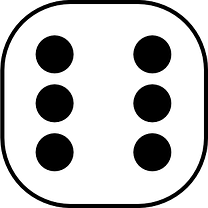
\includegraphics[width=0.1in]{Dice/die6} .

\(X\) is discrete with \(\mathcal{R}_X = \{0, 1, 2\}\).
\(Y\) is discrete with a countably infinite range \(\mathcal{R}_Y = \{ 1, 2, 3, \dots\}\).

The range is \(\mathcal{R}_{X\times Y} = \{ (x, y): 0 \le x \le 2, y = 1, 2, 3, \dots\}\).
\end{example}

As with the univariate case, the description and language for the probability function are different, depending on whether the random variables~\(X\) and~\(Y\) are discrete or continuous case (though the ideas remain similar).
While not common, the case where one variable, say~\(X\), is continuous and the other, say~\(Y\), is discrete also occurs.
We defer this case until Sect.~\ref{MixedJointPF}.

\begin{definition}[Discrete bivariate distribution function]
\protect\hypertarget{def:BivariateProbFunction}{}\label{def:BivariateProbFunction}Let \((X, Y)\) be a \(2\)-dimensional random variable where~\(X\) and~\(Y\) are both discrete random variables.
With each \((x_i, y_j)\) we associate a number \(p_{X, Y}(x_i, y_j)\) representing \(\Pr(X = x_i, Y = y_j)\) and satisfying
\begin{align}
   p_{X, Y}(x_i, y_j) &\geq 0, \text{ for all } (x_i, y_j)  \\
   \sum_{j = 1}^{\infty} \sum_{i = 1}^{\infty} p_{X, Y}(x_i, y_j)
   &= 1.
   \label{eq:BivariateProbFunctionDiscrete}
\end{align}
Then the function \(p_{X, Y}(x, y)\), defined for all \((x_i, y_j) \in R\) is called the \emph{probability function} of \((X, Y)\).
Also,
\[
   \{x_i, y_j, p_{X,Y}(x_i, y_j); i, j = 1, 2, \ldots\} 
\]
is called the \emph{probability distribution} of \((X, Y)\).
\end{definition}

\begin{definition}[Continuous bivariate distribution function]
\protect\hypertarget{def:BivariateProbFunctionCont}{}\label{def:BivariateProbFunctionCont}Let \((X, Y)\) be a \(2\)-dimensional random variable where~\(X\) and~\(Y\) are both continuous random variables.
The \emph{joint probability density function}, \(f_{X, Y}\), is a function satisfying
\begin{align}
   f_{X, Y}(x, y) &\geq 0, \text{ for all } (x, y) \in R, \\
   \int \!\! \int_{R} f_{X, Y}(x, y) \, dx \, dy &= 1.
\end{align}
\end{definition}

The second of these indicates that the \emph{volume} under the surface \(f_{X, Y}(x, y)\) is one.
Also, for \(\Delta x, \Delta y\) sufficiently small,
\begin{equation}
   f_{X, Y}(x, y) \, \Delta x \Delta y \approx \Pr(x \leq X \leq x + \Delta x, y \leq Y \leq y + \Delta y).
\end{equation}
Probabilities of events can be determined by the probability function or the probability density function as follows.

\begin{definition}[Bivariate distribution probabilities]
\protect\hypertarget{def:BVProbabilities}{}\label{def:BVProbabilities}For any event~\(A\), \emph{the probability of~\(A\)} is given by
\begin{align*}
   \Pr(A) 
   &= \sum_{(x, y) \in A} p(x, y),                       &&\text{for $(X, Y)$ discrete;}\\
   \Pr(A)
   &= \int \!\! \int_{(x, y) \in A}f(x, y) \, dx \, dy   &&\text{for $(X, Y)$ continuous.}
\end{align*}
\end{definition}

As in the univariate case, a bivariate distribution can be given in various ways:

\begin{itemize}
\tightlist
\item
  by enumerating the range and corresponding probabilities;
\item
  by a formula; or
\item
  a graph; or
\item
  by a table.
\end{itemize}

\begin{example}[Bivariate discrete]
\protect\hypertarget{exm:BVDiscrete2}{}\label{exm:BVDiscrete2}Consider the following discrete distribution where probabilities \(\Pr(X = x, Y = y)\) are shown as a graph
(Fig.~\ref{fig:Bivar1graphlatex})
and a table (Table~\ref{tab:Bivar1}).

To find \(\Pr(X + Y = 2)\):
\begin{align*}
   \Pr(X + Y = 2)
   &=\Pr\big(\{X = 2, Y = 0\} \text{ or } 
             \{X = 1, Y = 1\} \text{ or } 
             \{X = 0, Y = 2\}\big)\\
   &= \Pr(X = 2, Y = 0) \, + 
      \, \Pr(X = 1, Y = 1) \, + 
      \, \Pr(X = 0, Y = 2)\\
   &= \frac{9}{42} \ + \ \frac{12}{42} \ + \ \frac{12}{42} 
   = \frac{33}{42}.
\end{align*}
\end{example}

\begin{figure}

{\centering \includegraphics[width=0.5\linewidth]{05-Bivariate_files/figure-latex/Bivar1graphlatex-1} 

}

\caption{A bivariate discrete probability function.}\label{fig:Bivar1graphlatex}
\end{figure}

\begin{table}
\centering
\caption{\label{tab:Bivar1}A bivariate discrete probability function}
\centering
\fontsize{10}{12}\selectfont
\begin{tabular}[t]{lrrr}
\toprule
\textbf{ } & \textbf{$x = 0$} & \textbf{$x = 1$} & \textbf{$x = 2$}\\
\midrule
$y = 0$ & $1/42$ & $4/42$ & $12/42$\\
$y = 1$ & $4/42$ & $12/42$ & $0$\\
$y = 2$ & $9/42$ & $0$ & $0$\\
\bottomrule
\end{tabular}
\end{table}

\begin{example}[Bivariate uniform distribution]
\protect\hypertarget{exm:BVContinuousUnif}{}\label{exm:BVContinuousUnif}Consider the following continuous bivariate distribution with joint PDF
\[
   f_{X, Y}(x, y) = 1, \quad \text{for $0 \leq x \leq 1$ and $0 \leq y \leq 1$}.
\]
This is sometimes called the \emph{bivariate continuous uniform distribution}\index{Bivariate continuous uniform distribution}
(Fig.~\ref{fig:BVCont3}).
The \emph{volume} under the surface is one.

To find \(\Pr(0 \leq x \leq \frac{1}{2}, 0 \leq y \leq \frac{1}{2})\), find the volume above the square with vertices \((0, 0), (0, 1/2), (1/2, 0), (1/2, 1/2)\).
Hence the probability is~\(1/4\).
\end{example}

\begin{figure}

{\centering \includegraphics[width=0.6\linewidth]{05-Bivariate_files/figure-latex/BVCont3-1} 

}

\caption{The bivariate continuous uniform distribution.}\label{fig:BVCont3}
\end{figure}

\begin{example}[Bivariate discrete]
\protect\hypertarget{exm:BVDiscrete3}{}\label{exm:BVDiscrete3}Consider a random process where \emph{two} coins are tossed, and \emph{one} die is rolled simultaneously (Example~\ref{exm:BVDiscreteEG}).
Let~\(X\) be the number of heads that show on the two coins, and~\(Y\) the number on the die.

Since the toss of the coin and the roll of the die are independent, the probabilities are computed as follows:
\begin{align*}
   \Pr(X = 0, Y = 1) 
   &= \Pr(X = 0) \times \Pr(Y = 1) = \frac{1}{4}\times\frac{1}{6} = \frac{1}{24};\\
   \Pr(X = 1, Y = 2) 
   &= \Pr(X = 1) \times \Pr(Y = 2) = \frac{1}{2}\times\frac{1}{6} = \frac{1}{12};
\end{align*}
and so on.
The complete joint probability function can be displayed in a graph (often tricky), a function, or a table (Table~\ref{tab:JointPF}).
Here, the joint pf could be given as the function
\[
   p_{X, Y}(x, y) =
      \begin{cases}
         \left(\frac{1}{12}\right) 0.5^{|x - 1|} & \text{for $(x, y)\in S$ defined earlier};\\
         0                                         & \text{elsewhere.}
      \end{cases}
\]
\end{example}

\begin{table}
\centering
\caption{\label{tab:JointPF}The joint pf for Example \ref{exm:BVDiscrete3}}
\centering
\fontsize{10}{12}\selectfont
\begin{tabular}[t]{>{}rrrrrrrr}
\toprule
\textbf{} & \textbf{$Y = 1$} & \textbf{$Y = 2$} & \textbf{$Y = 3$} & \textbf{$Y = 4$} & \textbf{$Y = 5$} & \textbf{$Y = 6$} & \textbf{Total}\\
\midrule
\textbf{$X = 0$} & $1/24$ & $1/24$ & $1/24$ & $1/24$ & $1/24$ & $1/24$ & $1/4$\\
\textbf{$X = 1$} & $1/12$ & $1/12$ & $1/12$ & $1/12$ & $1/12$ & $1/12$ & $1/2$\\
\textbf{$X = 2$} & $1/24$ & $1/24$ & $1/24$ & $1/24$ & $1/24$ & $1/24$ & $1/4$\\
\midrule
\textbf{Total} & $1/6$ & $1/6$ & $1/6$ & $1/6$ & $1/6$ & $1/6$ & $1$\\
\bottomrule
\end{tabular}
\end{table}

\begin{example}[Two dice]
\protect\hypertarget{exm:BVDiscreteTwoDice}{}\label{exm:BVDiscreteTwoDice}Consider the bivariate discrete distribution which results when two dice are thrown.

Let~\(X\) be the number of times a
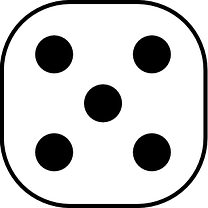
\includegraphics[width=0.1in]{Dice/die5} appears, and~\(Y\) the number of times a
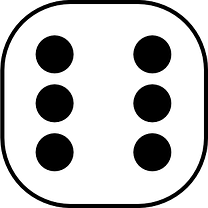
\includegraphics[width=0.1in]{Dice/die6} appears.
The ranges of~\(X\) and~\(Y\) are \(\mathcal{R}_X = \{0, 1 ,2 \}\), \(\mathcal{R}_Y = \{0, 1, 2\}\) and the range for the random process is the Cartesian product of~\(\mathcal{R}_X\) and~\(\mathcal{R}_Y\), understanding that some of the resulting points may have probability zero.
The probabilities in Table~\ref{tab:BVTwoDice} are \(\Pr(X = x, Y = y)\) for the \((x, y)\) pairs in the range.

The probabilities are found by realising we really have two repetitions of a simple random process with three possible outcomes, \(\{5, 6, (\text{$5$ or $6$})^c \}\), with probabilities \(\frac{1}{6}, \frac{1}{6}, \frac{2}{3}\), the same for each repetition.
(Recall: \(\overline{\text{$5$ or $6$}}\) means `not 5 or 6'; see Def.~\ref{def:IntersectionUnionSubset}.)
Of course the event \(X = 2, Y = 1\) cannot occur in two trials, so has probability zero.
\end{example}

\begin{table}
\centering
\caption{\label{tab:BVTwoDice}Joint probability distribution for Example \ref{exm:BVDiscreteTwoDice}.}
\centering
\fontsize{10}{12}\selectfont
\begin{tabular}[t]{>{}rrrr}
\toprule
\textbf{} & \textbf{$x = 1$} & \textbf{$x = 2$} & \textbf{$x = 3$}\\
\midrule
\textbf{$y = 0$} & $(2/3)^2$ & $2(1/6)(2/3)$ & $(1/6)^2$\\
\textbf{$y = 1$} & $2(1/6)(2/3)$ & $2(1/6)(1/6)$ & $0$\\
\textbf{$y = 2$} & $(1/6)^2$ & $0$ & $0$\\
\bottomrule
\end{tabular}
\end{table}

Example~\ref{exm:BVDiscreteTwoDice} is a special case of the \emph{multinomial distribution}\index{Multinomial distribution} (a generalisation of the binomial distribution), described later (Sect.~\ref{MultinomialDistribution}).

\begin{example}[Banks]
\protect\hypertarget{exm:BVDiscreteBank}{}\label{exm:BVDiscreteBank}A bank operates both an ATM and a teller.
On a randomly selected day, let~\(X_1\) be the proportion of time the ATM is in use (at least one customer is being served or waiting to be served), and~\(X_2\) is the proportion of time the teller is busy.

The set of possible values for~\(X_1\) and~\(X_2\) is the rectangle \(R = \{(x_1, x_2)\mid 0 \le x_1 \le 1, 0 \le x_2 \le 1\}\).
From experience, the joint PDF of \((X_1, X_2)\) is
\[
   f_{X_1, X_2}(x_1, x_2) =
      \begin{cases}
        c(x_1 + x_2^2) & \text{for $0\le x_1\le 1$; $0\le x_2\le 1$};\\
        0 & \text{elsewhere.}
    \end{cases}
\]

To determine a value for~\(c\), first see that if \(f_{X_1, X_2}(x_1, x_2) \ge 0\) for all~\(x_1\) and~\(x_2\), then \(c > 0\); and
\[
   \int_{-\infty}^{\infty}\!\int_{-\infty}^{\infty} f_{X_1, X_2}(x_1, x_2)\, dx_1\,dx_2 = 1.
\]
Hence,
\begin{align*}
    \int_{-\infty}^{\infty}\!\int_{-\infty}^{\infty} f_{X_1, X_2}(x_1, x_2)\, dx_1\,dx_2
    &= \int_{0}^{1}\!\!\!\int_{0}^{1} f_{X_1, X_2}(x_1, x_2)\, dx_1\,dx_2 \\
    &= c \int_{x_2 = 0}^{1}\left\{\int_{x_1=0}^{1} (x_1 + x_2^2)\, dx_1\right\} dx_2\\
    &= c (1/2 + 1/3) = 5c/6,
\end{align*}
and so \(c = 6/5\).

Consider the probability \emph{neither} facility is busy more than half the time.
Mathematically, the question is asking to find \(\Pr( 0\le X_1\le 0.5, 0\le X_2\le 0.5)\); call this event~\(A\).
Then,
\begin{align*}
   \Pr(A)
   &= \int_{0}^{0.5}\,\,\, \int_{0}^{0.5} f_{X_1, X_2}(x_1, x_2)\, dx_1\, dx_2 \\
   &= \frac{6}{5} \int_{0}^{0.5}\left\{\int_{0}^{0.5} x_1 + x_2^2\, dx_1\right\} dx_2 \\
   &= \frac{6}{5} \int_{0}^{0.5} (1/8 + x_2^2/2) \, dx_2 = 1/10.
\end{align*}
\end{example}

\section{Joint distribution function}\label{BivariateDistributionFunction}

The (cumulative) distribution function represents a sum of probabilities, or a volume under a surface, is denoted by \(F_{X, Y}(x, y)\), and defined as follows.

\begin{example}[Bivariate distribution function]
\protect\hypertarget{exm:BVDistributionFN}{}\label{exm:BVDistributionFN}The \emph{bivariate distribution function} is
\begin{align}
   F(x, y)
   &= \Pr(X \leq x, \, Y \leq y),                           & \text{for $(X,Y)$ discrete;}
   \label{eq:BivarXYdiscrete}\\
   F(x, y)
   &= \int_{-\infty}^y \int_{-\infty}^x f(u,v) \, du \, dv, & \text{for $(X,Y)$ continuous.}
   \label{eq:BivarXYcontinuous}
\end{align}
\end{example}

\begin{example}[Bivariate discrete]
\protect\hypertarget{exm:BVDiscrete3DF}{}\label{exm:BVDiscrete3DF}Consider the random process in Example~\ref{exm:BVDiscrete3}, where \emph{two} coins are tossed, and \emph{one} die is rolled (simultaneously).
The probability function is given in Table~\ref{tab:JointPF}.

The complete joint distribution function is given in Table~\ref{tab:Bivar2TableDF}, and complicated even for this simple case.
As an example, the joint df at \((1, 2)\) would be computed as follows:
\begin{align*}
   F_{X, Y}(1, 2)
   &= \displaystyle \sum_{x\le1} \,  \sum_{y\le 2} p_{X, Y}(x, y)\\
   &= p_{X, Y}(0, 1) + p_{X, Y}(0, 2) +  p_{X, Y}(1, 1) + p_{X, Y}(1, 2) \\
   &= 1/24 + 1/24 + 1/12 + 1/12 = 6/24.
\end{align*}
\end{example}

\begin{table}
\centering
\caption{\label{tab:Bivar2TableDF}The bivariate probability function for $X$ and $Y$.}
\centering
\fontsize{10}{12}\selectfont
\begin{tabular}[t]{>{}rrrrrrrr}
\toprule
\textbf{} & \textbf{$y < 1$} & \textbf{$y \le 1$} & \textbf{$y \le 2$} & \textbf{$y \le 3$} & \textbf{$y \le 4$} & \textbf{$y \le 5$} & \textbf{$y \le 6$}\\
\midrule
\textbf{$x\lt 0$} & 0 & 0 & 0 & 0 & 0 & 0 & 0\\
\textbf{$x\le 0$} & 0 & $1/24$ & $2/24$ & $3/24$ & $4/24$ & $5/24$ & $6/24$\\
\textbf{$x\le 1$} & 0 & $3/24$ & $6/24$ & $9/24$ & $12/24$ & $15/24$ & $18/24$\\
\textbf{$x\le 2$} & 0 & $4/24$ & $8/24$ & $12/24$ & $16/24$ & $20/24$ & $24/24$\\
\bottomrule
\end{tabular}
\end{table}

\begin{example}[Bivariate continuous]
\protect\hypertarget{exm:BVCont}{}\label{exm:BVCont}From Example~\ref{exm:BVDiscreteBank},
\begin{align*}
   F_{X, Y}(x, y)
   &= \frac{6}{5} \int_0^{x} \int_0^{y} (t_1 + t_2^2)\, dt_2 dt_1 \\
   &= \frac{6}{5} \int_0^{x} (t_1 t_2 + t_2^3/3)\Big|_{t_2 = 0}^{t_2 = y} \, dt_1 \\
   &= \frac{6}{5} \int_0^{x} (t_1 y + x_2^3/3)\, dt_1 \\
   &= \frac{6}{5} \left( \frac{x y}{2} + \frac{x y^3}{3}\right)
\end{align*}
for \(0 < x < 1\) and \(0 < y < 1\).
So
\[
   F_{X, Y}(x, y)
   = \begin{cases}
      0 & \text{if $x < 0$ or $y < 0$};\\
      \frac{6}{5} \left( x y/2 + x x_2^3/3\right) & \text{if $0 \le x \le 1$ and $0 \le y \le 1$};\\
      1 & \text{if $x > 1$ and $y > 1$}.
     \end{cases}
\]
\end{example}

\section{Marginal distributions}\label{MarginalDistributions}

With each two-dimensional random variable \((X, Y)\) two one-dimensional random variables, namely~\(X\) and~\(Y\), can be described.
We can find the probability distributions of each of~\(X\) and~\(Y\) separately.

In the case of a discrete random vector \((X, Y)\), the event \(X = x_i\) is the union of the mutually exclusive events
\[
   \{X = x_i, Y = y_1\}, \{\ X = x_i, Y = y_2\}, \{X = x_i, Y = y_3\}, \dots
\]
Thus,
\begin{align*}
   \Pr(X = x_i)
   &= \Pr(X = x_i, Y = y_1) + \Pr(X = x_i, Y = y_2) + \dots \\
   &= \sum_jp_{X, Y}(x_i, y_j),
\end{align*}
where the notation means to sum over all values given under the summation sign.
Hence, the marginal distributions can be defined when \((X, Y)\) is a discrete random vector.

\begin{definition}[Bivariate discrete marginal distributions]
\protect\hypertarget{def:BVDiscreteMarginal}{}\label{def:BVDiscreteMarginal}Given \((X, Y)\) with joint discrete probability function \(p(x, y)\), the \emph{marginal probability functions} of~\(X\) and~\(Y\) are, respectively
\begin{equation}
   \Pr(X = x) = \sum_{y}p_{X, Y}(x, y)
   \quad\text{and}\quad
   \Pr(Y = y) = \sum_{x}p_{X, Y}(x, y).
   \label{eq:BivariateMarginal}
\end{equation}
\end{definition}

An analogous definition exists when the random vector \((X,Y)\) is continuous.

\begin{definition}[Bivariate continuous marginal distributions]
\protect\hypertarget{def:BVContMarginal}{}\label{def:BVContMarginal}If \((X, Y)\) has joint continuous PDF \(f(x, y)\), the \emph{marginal PDFs} of~\(X\) and~\(Y\), denoted by \(f_X(x)\), \(f_Y(y)\) respectively, are
\[
   f_X(x) = \int_{-\infty}^{\infty}f(x,y) \, dy 
   \quad\text{and}\quad
   f_Y(y) = \int_{-\infty}^{\infty}f(x,y) \, dx.
\]
\end{definition}

\begin{example}[Bivariate continuous marginal distributions]
\protect\hypertarget{exm:BVContinuousMarginal}{}\label{exm:BVContinuousMarginal}The joint probability density functions of~\(X\) and~\(Y\) is
\[
   f(x, y) = 
   \left\{
   \begin{array}{ll}
       \frac{1}{3} (3x^2 + xy), & 0 \leq x \leq 1, \, 0 \leq y \leq 2;\\
       0 & \text{ elsewhere.} 
   \end{array} 
   \right.
\]
The marginal probability density functions for~\(X\) is
\begin{align*}
   f_X(x)
   = \int_0^2\left(x^2 + \frac{xy}{3}\right) dy 
   &= \left.x^2y + \frac{xy^2}{6}\right|_{y = 0}^2\\
   &= 2x^2 + \frac{2x}{3}\quad\text{for $0 \leq x \leq 1$}.
\end{align*}
Also,
\[
   f_Y(y)
   = \int_0^1\left(x^2 + \frac{xy}{3}\right)dx
   = \left.\frac{1}{3}x^3 + \frac{1}{6}x^2y\right|_{x = 0}^1.
\]
So \(\displaystyle f_Y(y) = \frac{1}{6}(2 + y)\), for \(0 \leq y \leq 2\).

Consider computing \(\Pr(Y < X)\); see Fig. \ref{fig:regionXY}; then
\begin{align*}
   \Pr(Y < X)
   &= \int \!\!\int_{\substack{(x, y) \in A\\ y < x}} f(x,y) \, dx \, dy \\
   &= \frac{1}{3}\int_0^1 \int_y^1(3x^2 + xy) \, dx \, dy\\
   &= \frac{1}{3} \int_0^1\left. x^3 + \frac{1}{2}x^2y\right|_y^1 dy\\
   &= \frac{1}{3} \int_0^1(1 + \frac{1}{2}y - \frac{3}{2}y^3) \, dy = \frac{7}{24}.
\end{align*}
\end{example}

\begin{figure}

{\centering 
\includegraphics[width=0.6\linewidth]{05-Bivariate_files/figure-latex/regionXY-1} 

}

\caption{The region where $Y < X$.}\label{fig:regionXY}
\end{figure}

\begin{example}[Bivariate discrete marginal distributions]
\protect\hypertarget{exm:BVDiscreteMarginal2}{}\label{exm:BVDiscreteMarginal2}Recall Example~\ref{exm:BVDiscreteTwoDice}, where two dice are rolled.
We can find the marginal distributions of~\(X\) and~\(Y\) (Table~\ref{tab:Marginals}).
The probabilities in the first row (where \(Y = 0\)), for instance, are summed and appear as the first term in the final column; this is the marginal distribution for \(Y = 0\).
Similarly for the other rows.

Recalling that~\(X\) is the number of times a

\includegraphics[width=0.1in]{Dice/die1} is rolled when two dice are thrown, the distribution of~\(X\) should be \(\text{Bin}(2,  1/6\)); the probabilities given in the last row of the table agree with this.
That is,
\[
  \Pr(X = x) = \binom{2}{x}\left(\frac{1}{6}\right)^x \left(\frac{5}{6}\right)^{2 - x}
\]
for \(x = 0, 1, 2\).
Of course, the distribution of~\(Y\) is the same.
\end{example}

\begin{table}
\centering
\caption{\label{tab:Marginals}The marginal distributions.}
\centering
\fontsize{10}{12}\selectfont
\begin{tabular}[t]{>{}rrrrr}
\toprule
\textbf{} & \textbf{$x = 0$} & \textbf{$x = 1$} & \textbf{$x = 2$} & \textbf{$\Pr(Y = y)$}\\
\midrule
\textbf{$y = 0$} & $4/9$ & $2/9$ & $1/36$ & $25/36$\\
\textbf{$y = 1$} & $2/9$ & $1/18$ & $0$ & $10/36$\\
\textbf{$y = 2$} & $1/36$ & $0$ & $0$ & $1/36$\\
\midrule
\addlinespace
\textbf{$\Pr(X = x)$} & $25/36$ & $10/36$ & $1/36$ & $1$\\
\bottomrule
\end{tabular}
\end{table}

\begin{example}[Bivariate discrete marginal distributions]
\protect\hypertarget{exm:BVDiscreteMarginal3}{}\label{exm:BVDiscreteMarginal3}Consider again the random process in Example~\ref{exm:BVDiscrete3DF}.
From Table~\ref{tab:JointPF}, the marginal distribution for~\(X\) is found simply by summing over the values for~\(Y\) in the table.
When \(x = 0\),
\[
   p_{X}(0) = \sum_{y} p_{X, Y}(0, y) = 1/24 + 1/24 + 1/24 +\dots = 6/24.
\]
Likewise,
\begin{align*}
   p_{X}(1) &= \sum_{y} p_{X, Y}(1, y) = 6/12;\\
   p_{X}(2) &= \sum_{y} p_{X, Y}(2, y) = 6/24.
\end{align*}
So the marginal distribution of~\(X\) is
\[
   p_{X}(x) = 
   \begin{cases}
     1/4 & \text{if $x = 0$};\\
     1/2 & \text{if $x = 1$};\\
     1/4 & \text{if $x = 2$};\\
     0 & \text{otherwise}.\\
  \end{cases}
\]
This is equivalent to adding the row probabilities in Table~\ref{tab:JointPF}.
In this example, the marginal distribution is easily found from the total column of Table~\ref{tab:JointPF}.
\end{example}

\section{Conditional distributions}\label{ConditionalDistributions}

Consider \((X, Y)\) with joint probability function as in Example~\ref{exm:BVDiscrete2}, with marginal distributions of~\(X\) and~\(Y\) as shown in Table~\ref{tab:JointPFmarginals}.

\begin{table}
\centering
\caption{\label{tab:JointPFmarginals}A joint distribution with the marginal distributions.}
\centering
\fontsize{10}{12}\selectfont
\begin{tabular}[t]{>{}rrrrr}
\toprule
\textbf{} & \textbf{$x = 0$} & \textbf{$x = 1$} & \textbf{$x = 2$} & \textbf{$\Pr(Y = y)$}\\
\midrule
\textbf{$y = 0$} & $1/36$ & $1/6$ & $1/4$ & $4/9$\\
\textbf{$y = 1$} & $1/9$ & $1/3$ & $0$ & $4/9$\\
\textbf{$y = 2$} & $1/9$ & $0$ & $0$ & $1/9$\\
\midrule
\addlinespace
\textbf{$\Pr(X = x)$} & $1/4$ & $1/2$ & $1/4$ & $1$\\
\bottomrule
\end{tabular}
\end{table}

Suppose we want to evaluate the conditional probability \(\Pr(X = 1 \mid Y = 1)\).
We use that \(\Pr(A \mid B) = \Pr(A \cap B)/\Pr(B)\).
So
\[
   \Pr(X = 1 \mid Y = 1) 
   = \frac{\Pr(X = 1, Y = 1)}{\Pr(Y = 1)} 
   = \frac{1/3}{4/9}
   = \frac{3}{4}.
\]
So, for each \(x\in \mathcal{R}_X\) we could find \(\Pr(X = x, Y = 1)\) and this is then the \emph{conditional} distribution of~\(X\) given that \(Y = 1\).

\begin{definition}[Bivariate discrete conditional distributions]
\protect\hypertarget{def:BVDiscreteConditional}{}\label{def:BVDiscreteConditional}For a discrete random vector \((X, Y)\) with probability function \(p_{X, Y}(x, y)\) the \emph{conditional probability distribution} of~\(X\) given \(Y = y\) is defined by
\begin{align}
   p_{X \mid Y}(x \mid Y = y)
   &= \Pr(X = x \mid Y = y)\\
   &= \frac{\Pr(X = x, Y = y)}{\Pr(Y = y)}\\
   &= \frac{p_{X, Y}(x, y)}{p_Y(y)}
\end{align}
for \(x \in \mathcal{R}_X\) and provided \(p_Y(y) > 0\).
\end{definition}

The continuous case is analogous.

\begin{definition}[Bivariate continuous marginal distributions]
\protect\hypertarget{def:BVContinuousMarginal}{}\label{def:BVContinuousMarginal}If \((X, Y)\) is a continuous \(2\)-dimensional random variable with joint PDF \(f_{X, Y}(x, y)\) and respective marginal probability density functions \(f_X(x)\), \(f_Y(y)\), then the \emph{conditional probability distribution} of~\(X\) given \(Y = y\) is defined by
\begin{equation}
   f_{X \mid Y}(x \mid Y = y)
   = \frac{f_{X, Y}(x, y)}{f_Y(y)}
\end{equation}
for \(x \in \mathcal{R}_X\) and provided \(f_Y(y) > 0\).
\end{definition}

The above conditional probability density functions satisfy the requirements for a univariate PDF; that is, \(f_{X \mid Y}(x \mid y) \ge 0\) for all~\(x\) and \(\int_0^\infty f_{X\mid Y}(x\mid y)\,dx = 1\).

\begin{example}[Bivariate continuous marginal distributions]
\protect\hypertarget{exm:BVcontinuousMarginal2}{}\label{exm:BVcontinuousMarginal2}In Example \ref{exm:BVContinuousMarginal}, the joint PDF of~\(X\) and~\(Y\) considered was
\[
   f_{X,Y}(x,y) = 
   \begin{cases}
      \frac{1}{3}(3x^2 + xy)  & \text{for $0 \leq x \leq 1$ and $0 \leq y \leq 2$};\\
      0                       & \text{elsewhere}. 
   \end{cases} 
\]
The marginal probability density functions of~\(X\) and~\(Y\) are
\begin{align*}
   f_X(x) &= 2x^2 + \frac{2}{3}x \quad\text{for $0 \leq x \leq 1$}; \\
   f_Y(y) &= \frac{1}{6}(2 + y) \quad \text{for $0 \leq y \leq 2$}.
\end{align*}
Hence, the conditional distribution of \(X \mid Y = y\) is
\[
   f_{X\mid Y}(x \mid Y = y) 
   = \frac{(3x^2 + xy)/3}{(2 + y)/6}
   = \frac{2x(3x + y)}{2 + y} \quad\text{for $0 \leq x \leq 1$},
\]
and the conditional distribution of \(Y \mid X = x\) is
\[
   f_{Y \mid X}(y \mid X = x) 
   = \frac{3x + y}{2(3x + 1)}\quad\text{for $0 \leq y \leq 2$}.
\]
Both these conditional density functions are valid density functions (verify!).

The marginal distribution for~\(Y\), and two conditional distributions of~\(Y\) (given \(X = 0.1\) and \(X = 0.9\)) are shown in Fig.~\ref{fig:MargCondY}.
\end{example}

\begin{figure}

{\centering 
\includegraphics[width=1\linewidth]{05-Bivariate_files/figure-latex/MargCondY-1} 

}

\caption{The marginal distribution of $Y$ (left panel), and the conditional distribution of $Y$ for $X = 0$ (centre panel) and $X = 1$ (right panel).}\label{fig:MargCondY}
\end{figure}

To interpret the conditional distribution, for example \(f_{X \mid Y = y}(x \mid y)\), consider slicing through the surface \(f_{X, Y}(x, y)\) with the plane \(y = c\) say, for~\(c\) a constant
(Fig.~\ref{fig:BivarConditionala}).
The intersection of the plane with the surface, will be proportional to a \(1\)-dimensional PDF.
This is \(f_{X, Y}(x, c)\), which will not, in general, be a density function since the area under this curve will be \(f_Y(c)\).
Dividing by the constant \(f_Y(c)\) ensures the area under \(\displaystyle\frac{f_{X,Y}(x,c)}{f_Y(c)}\) is one.
This is a one-dimensional PDF, of~\(X\) given \(Y = c\); that is \(f_{X \mid Y = c}(x\mid c)\).

\begin{figure}

{\centering \includegraphics[width=0.55\linewidth]{05-Bivariate_files/figure-latex/BivarJointa-1} 

}

\caption{A bivariate distribution.}\label{fig:BivarJointa}
\end{figure}

\begin{figure}

{\centering \includegraphics[width=0.55\linewidth]{05-Bivariate_files/figure-latex/BivarConditionala-1} 

}

\caption{A bivariate distribution, sliced at $Y =  1$, showing the conditional distribution of $X$ when $Y = 0.5$.}\label{fig:BivarConditionala}
\end{figure}

\begin{example}[Bivariate discrete conditional distributions]
\protect\hypertarget{exm:BVDiscreteConditional}{}\label{exm:BVDiscreteConditional}Consider again the random process in Example~\ref{exm:BVDiscrete3}.
The conditional distribution for~\(Y\) given \(X = 0\) can be found from Table~\ref{tab:JointPFmarginals}.
First, \(p_{X}(x)\), is needed, which was found in Example~\ref{exm:BVDiscreteMarginal3}.
Then,
\begin{align*}
   p_{Y\mid X}(y\mid X = 0)
   &= \frac{p_{X, Y}(0, y)}{p_{X}(0)} \\
   &= \frac{p_{X, Y}(0, y)}{1/4},
\end{align*}
from which we can deduce
\[
   p_{Y \mid X = 0}(y \mid X = 0) =
   \begin{cases}
      \frac{1/24}{1/4} = 1/6 & \text{for $y = 1$};\\
      \frac{1/24}{1/4} = 1/6 & \text{for $y = 2$};\\
      \frac{1/24}{1/4} = 1/6 & \text{for $y = 3$};\\
      \frac{1/24}{1/4} = 1/6 & \text{for $y = 4$};\\
      \frac{1/24}{1/4} = 1/6 & \text{for $y = 5$};\\
      \frac{1/24}{1/4} = 1/6 & \text{for $y = 6$}.\\
   \end{cases}
\]
The conditional distribution \(p_{Y\mid X = x}(y\mid x)\) is a probability function for~\(Y\) (verify!).
Since~\(Y\) was the number of the top face of the die, this is exactly as we should expect.
\end{example}

\section{Independent random variables}\label{BivariateIndependentRVs}

Recall that events~\(A\) and~\(B\) are independent if, and only if,
\[
   \Pr(A \cap B) = \Pr(A)\Pr(B).
\]
An analogous definition applies for random variables.

\begin{definition}[Independent random variables]
\protect\hypertarget{def:Independent}{}\label{def:Independent}The random variables~\(X\) and~\(Y\) with joint distribution function~\(F_{X, Y}\) and marginal distribution functions~\(F_X\) and~\(F_Y\) are \emph{independent} if, and only if,
\begin{equation}
   F_{X, Y}(x, y) = F_X(x) \times F_Y(y)
\end{equation}
for all~\(x\) and~\(y\).

If~\(X\) and~\(Y\) are not independent they are \emph{dependent}, or \emph{not independent}.
\end{definition}

The following theorem is often used to establish independence or dependence of random variables.
The proof is omitted.

\begin{theorem}
The discrete random variables~\(X\) and~\(Y\) with joint probability function \(p_{X, Y}(x, y)\) and marginal distributions \(p_X(x)\) and \(p_Y(y)\) are \emph{independent} if, and only if,
\begin{equation}
   p_{X, Y}(x, y) = p_X(x) \times p_Y(y) \text{ for every }(x, y) \in \mathcal{R}_{X \times Y}.
      \label{eq:IndependentDiscretervs}
\end{equation}
The continuous random variables \((X, Y)\) with joint PDF \(f_{X, Y}\) and marginal PDFs \(f_X\) and \(f_Y\) are \emph{independent} if, and only if,
\begin{equation}
   f_{X, Y}(x, y) = f_X(x)\times f_Y(y)
\end{equation}
for all~\(x\) and~\(y\).
\end{theorem}

To show independence for continuous random variables (and analogously for discrete random variables) we must show \(f_{X, Y}(x, y) = f_X(x)\times f_Y(y)\) for \emph{all} pairs \((x, y)\).
If \(f_{X, Y}(x, y)\neq f_X(x)\times f_Y(y)\), even for any one particular pair of \((x, y)\), then~\(X\) and~\(Y\) are dependent.

\begin{example}[Bivariate discrete: Independence]
\protect\hypertarget{exm:BVDiscreteIndependence}{}\label{exm:BVDiscreteIndependence}The random variables~\(X\) and~\(Y\) have the joint probability distribution shown in Table~\ref{tab:Joint2}.
Summing across rows, the marginal probability function of~\(Y\) is:
\[
   p_Y(y) = 
   \begin{cases}
      1/6  & \text{for $y = 1$};\\
      1/3  & \text{for $y = 2$};\\
      1/2  & \text{for $y = 3$}.
   \end{cases}
\]
To determine if~\(X\) and~\(Y\) are independent, the marginal probability function of~\(X\) is also needed:
\[
   p_X(x) = 
   \begin{cases}
      1/5  & \text{for $x = 1$};\\
      1/5  & \text{for $x = 2$};\\
      2/5  & \text{for $x = 3$};\\
      1/5  & \text{for $x = 4$}.
   \end{cases}
\]
Clearly, Eq.~\eqref{eq:IndependentDiscretervs} is satisfied for all pairs \((x, y)\), so~\(X\) and~\(Y\) are independent.
\end{example}

\begin{table}
\centering
\caption{\label{tab:Joint2}A joint probability function.}
\centering
\fontsize{10}{12}\selectfont
\begin{tabular}[t]{>{}rrrrr}
\toprule
\textbf{} & \textbf{$x = 1$} & \textbf{$x = 2$} & \textbf{$x = 3$} & \textbf{$x = 4$}\\
\midrule
\textbf{$y = 1$} & $1/30$ & $1/30$ & $2/30$ & $1/30$\\
\textbf{$y = 2$} & $2/30$ & $2/30$ & $4/30$ & $2/30$\\
\textbf{$y = 3$} & $3/30$ & $3/30$ & $6/30$ & $3/30$\\
\bottomrule
\end{tabular}
\end{table}

\begin{example}[Bivariate continuous: independence]
\protect\hypertarget{exm:BVContinuousIndependence}{}\label{exm:BVContinuousIndependence}Consider the random variables~\(X\) and~\(Y\) with joint PDF
\[
   f_{X, Y}(x, y)
   = \begin{cases}
      4xy & \text{for $0 < x < 1$ and $0 < y < 1 $}\\
      0   & \text{elsewhere}.\\ 
   \end{cases}
\]
To show that~\(X\) and~\(Y\) are independent, the marginal distributions of~\(X\) and~\(Y\) are needed.
Now
\[
   f_X(x)
   = \int_0^1 4xy \, dy = 2x\quad\text{for $0 < x < 1$}.
\]
Similarly \(f_Y(y) = 2y\) for \(0 < y < 1\).
Thus we have \(f_X(x) \cdot f_Y(y) = f(x,y)\), so~\(X\) and~\(Y\) are independent.
\end{example}

\begin{example}[Bivariate discrete: independence]
\protect\hypertarget{exm:BVDiscreteIndependence2}{}\label{exm:BVDiscreteIndependence2}Consider again the random process in Example~\ref{exm:BVDiscrete3}.
The marginal distribution of~\(X\) was found in Example~\ref{exm:BVDiscreteMarginal3}.
The marginal distribution of~\(Y\) is (check!)
\[
   p_{Y}(y) =
   \begin{cases}
      \frac{1/24}{1/4} = 1/6 & \text{for $y = 1$};\\
      \frac{1/24}{1/4} = 1/6 & \text{for $y = 2$};\\
      \frac{1/24}{1/4} = 1/6 & \text{for $y = 3$};\\
      \frac{1/24}{1/4} = 1/6 & \text{for $y = 4$};\\
      \frac{1/24}{1/4} = 1/6 & \text{for $y = 5$};\\
      \frac{1/24}{1/4} = 1/6 & \text{for $y = 6$}.\\
   \end{cases}
\]
To determine if~\(X\) and~\(Y\) are independent, \emph{each}~\(x\) and~\(y\) pair must be considered.
As an example, we see
\begin{align*}
   p_{X}(0) \times p_{Y}(1) = 1/4 \times 1/6 = 1/24 &= p_{X, Y}(0, 1);\\
   p_{X}(0) \times p_{Y}(2) = 1/4 \times 1/6 = 1/24 &= p_{X, Y}(0, 2);\\
   p_{X}(1) \times p_{Y}(1) = 1/2 \times 1/6 = 1/12 &= p_{X, Y}(1, 1);\\
   p_{X}(2) \times p_{Y}(1) = 1/4 \times 1/6 = 1/24 &= p_{X, Y}(2, 1).
\end{align*}
This is true for all pairs, and so~\(X\) and~\(Y\) are independent random variables.
Independence is, however, obvious from the description of the random process (Example~\ref{exm:BVDiscreteEG}), and is easily seen from Table~\ref{tab:JointPF}.
\end{example}

\begin{example}[Bivariate continuous: independence]
\protect\hypertarget{exm:BVContinuousIndependence2}{}\label{exm:BVContinuousIndependence2}Consider the continuous random variables~\(X\) and~\(Y\) with joint PDF
\[
   f_{X, Y}(x, y)  =
   \begin{cases}
      \frac{2}{7}(x + 2y) & \text{for $0 < x < 1$ and $1 < y < 2$};\\
      0 & \text{elsewhere.}
   \end{cases}
\]
The marginal distribution of~\(X\) is
\[
   f_{X}(x)
   = \int_1^2 \frac{2}{7}(x + 2y)\,dy\\
   =   \frac{2}{7}(x + 3)
\]
for \(0 < x < 1\) (and zero elsewhere).
Likewise, the marginal distribution of~\(Y\) is
\[
   f_{Y}(y)
   = \frac{2}{7}(x^2/2 + 2 x y)\Big|_{x = 0}^1
   = \frac{1}{7}(1 + 4y)
\]
for \(1 < y < 2\) (and zero elsewhere).
(Both the marginal distributions must be valid density functions; verify!)
Since
\[
   f_{X}(x) \times f_{Y}(y) = \frac{2}{49}(x + 3)(1 + 4y) \ne f_{X, Y}(x, y),
\]
the random variables~\(X\) and~\(Y\) are \emph{not independent}.

The conditional distribution of~\(X\) given \(Y = y\) is
\begin{align*}
   f_{X \mid Y = y}(x \mid y)
   &= \frac{ f_{X, Y}(x, y)}{ f_{Y}(y)} \\
   &= \frac{ (2/7) (x + 2y)}{ (1/7)(1 + 4y)}\\
   &= \frac{ 2 (x + 2y)}{ 1 + 4y}
\end{align*}
for \(0 < x < 1\) and any given value of \(1 < y < 2\).
(Again, this conditional density must be a valid probability density function.)
So, for example,
\[
   f_{X \mid Y}(x\mid Y = 1.5)
   = \frac{ 2 (x + 2\times 1.5)}{ 1 + (4\times 1.5)}
   = \frac{2}{7}(x + 3)
\]
for \(0 < x < 1\) and is zero elsewhere.
And,
\[
   f_{X\mid Y}(x \mid Y = 1)
   = \frac{ 2 (x + 2\times 1)}{ 1 + (4\times 1)}
   = \frac{2}{5}(x + 2)
\]
for \(0 < x < 1\) and is zero elsewhere.
Since the distribution of~\(X\) depends on the given value of~\(Y\), \(X\) and~\(Y\) are \emph{not} independent.
\end{example}

\begin{example}[Bivariate continuous: independence]
\protect\hypertarget{exm:BVContinuousIndependence3}{}\label{exm:BVContinuousIndependence3}Consider the two continuous random variables~\(X\) and~\(Y\) with joint probability function
\[
   f_{X, Y}(x, y)=
   \begin{cases}
      2(x + y) & \text{for $0 < x < y < 1$};\\
      0        & \text{elsewhere}.
   \end{cases}
\]
A diagram of the region over which~\(X\) and~\(Y\) are defined is shown in Fig.~\ref{fig:BVRegion}.
To determine if~\(X\) and~\(Y\) are independent, the two marginal distributions are needed.
For example:
\[
   f_{X}(x) = 1 + 2x - 3x^2\quad\text{for $0 < x < 1$}.
\]
Since the distribution of~\(X\) depends on the value of~\(Y\), this means~\(X\) and~\(Y\) are \emph{not independent}.
\end{example}

\begin{figure}

{\centering 
\includegraphics{05-Bivariate_files/figure-latex/BVRegion-1} 

}

\caption{The region over which $f_{X, Y}(x, y)$ is defined.}\label{fig:BVRegion}
\end{figure}

\section{Mixed joint probability functions}\label{MixedJointPF}

So far, the bivariate distributions have included the cases of two discrete or two continuous random variables.
However, it is also possible for one variable, say~\(X\), to be continuous and the other, say~\(Y\), to be discrete.

\begin{definition}[Mixed bivariate probability function]
\protect\hypertarget{def:BivariateProbFunctionMixed}{}\label{def:BivariateProbFunctionMixed}

Let \((X, Y)\) be a random vector where~\(X\) is \emph{continuous} with range \(S_X \subseteq \mathbb{R}\), and~\(Y\) is \emph{discrete} with range \(S_Y = \{y_1, y_2, \dots\}\).
The \emph{joint density--mass function} of \((X, Y)\) is defined on
\[
  \mathcal{R}_{X, Y} = S_X \times S_Y
\]
by
\[
  f_{X, Y}(x, y_j) 
  = f_{X \mid Y}(x \mid y_j) \cdot p_Y(y_j),
\]
where:

\begin{itemize}
\tightlist
\item
  \(p_Y(y_j) = \Pr(Y = y_j)\) is the probability \emph{mass} function of~\(Y\), and
\item
  \(f_{X \mid Y}(x \mid y_j)\) is the conditional \emph{density} function of~\(X\) given~\(Y = y_j\).
\end{itemize}

\end{definition}

Like all probability functions, the joint density--mass function is non-negative:
\[
  f_{X, Y}(x, y_j) \geq 0 \quad \text{for all $(x, y_j)\in\mathcal{R}_{X, Y}$}.
\]
In addition, the total probability is one:
\[
  \sum_{j\in S_Y} \int_{S_X} f_{X,Y}(x, y_j)\, dx = 1.
\]

The probability of any event \(A \subseteq S_X\) and \(y_j \in S_Y\) is
\[
  \Pr(X \in A, Y = y_j) = \int_A f_{X,Y}(x, y_j)\, dx.
\]

\begin{example}[Mixed random variable]
\protect\hypertarget{exm:MixedRV}{}\label{exm:MixedRV}Suppose a random vector \((X, Y)\) is defined so that \(Y \in \{1, 2\}\) with
\[
  p_Y(1) = 0.4, \quad p_Y(2) = 0.6.
\]
Conditional on \(Y = 1\), the probability density function of~\(X\) is
\[
  f_{X \mid Y}(x \mid Y = 1) = 
  \begin{cases}
    1 & 0 \le x \le 1, \\
    0 & \text{otherwise,}
  \end{cases}
\]
and conditional on \(Y = 2\), the probability density function of~\(X\) is
\[
  f_{X \mid Y}(x \mid Y = 2) 
  = 
  \begin{cases}
    1/2   & 0 \le x \le 2, \\
    0     & \text{otherwise.}
  \end{cases}
\]
Then the joint density--mass function is
\[
  f_{X, Y}(x, y) 
  = f_{X \mid Y}(x \mid y) \cdot p_Y(y)
\]
or, more explicitly:
\[
  f_{X, Y}(x, 1) =
  \begin{cases}
    0.4  & 0 \le x \le 1, \\
    0,   & \text{otherwise;}
\end{cases}
\quad
f_{X, Y}(x, 2) 
= 
\begin{cases}
  0.3 & 0 \le x \le 2, \\
  0   & \text{otherwise.}
\end{cases}
\]
Notice that
\[
  \sum_{y \in \{1,2\}} \int_{-\infty}^{\infty} f_{X,Y}(x,y)\, dx
  = \int_0^1 0.4 \, dx + \int_0^2 0.3 \, dx
  = 0.4 + 0.6 = 1
\]
as required.

Then, for instance, we can find \(\Pr(X \le 0.5, Y = 2)\):
\[
  \Pr(X \le 0.5, Y = 2) 
  = \int_0^{0.5} f_{X, Y}(x, 2)\, dx
  = \int_0^{0.5} 0.3\, dx
  = 0.15.
\]
\end{example}

\section{Numerical approaches}\label{BivariateNumerical}

\section{Exercises}\label{ChapBivariateExercises}

Selected answers appear in Sect.~\ref{AnswersChapBivariateExercises}.

\begin{exercise}
\protect\hypertarget{exr:DiscreteXY}{}\label{exr:DiscreteXY}

The discrete random variables~\(X\) and~\(Y\) have the joint probability function shown in Table~\ref{tab:TableXY}.

\begin{enumerate}
\def\labelenumi{\arabic{enumi}.}
\tightlist
\item
  Determine \(\Pr(X = 1, Y = 2)\)
\item
  Determine \(\Pr(X + Y \le 1)\).
\item
  Compute \(\Pr(X > Y)\).
\item
  Find the marginal probability function of~\(X\).
\item
  Find the probability function of \(Y \mid X = 1\).
\end{enumerate}

\end{exercise}

\begin{table}

\caption{\label{tab:TableXY}The joint probability mass function of $X$ and $Y$.}
\centering
\begin{tabular}[t]{rrrr}
\toprule
\textbf{} & \textbf{$Y = 0$} & \textbf{$Y = 1$} & \textbf{$Y = 2$}\\
\midrule
$X = 0$ & $1/12$ & $1/6$ & $1/24$\\
$X = 1$ & $1/4$ & $1/4$ & $5/24$\\
\bottomrule
\end{tabular}
\end{table}

\begin{exercise}
\protect\hypertarget{exr:DiscreteXY2}{}\label{exr:DiscreteXY2}

The discrete random variables~\(X\) and~\(Y\) have the joint probability function shown in Table~\ref{tab:TableXY2}.

\begin{enumerate}
\def\labelenumi{\arabic{enumi}.}
\tightlist
\item
  Determine \(\Pr(X < 3, Y = 0)\)
\item
  Determine \(\Pr(X + Y > 3)\).
\item
  Compute \(\Pr(X > (Y/2) )\).
\item
  Find the marginal probability function of~\(Y\).
\item
  Find the marginal probability function of~\(X\).
\item
  Find the probability function of \(Y \mid X = 1\).
\end{enumerate}

\end{exercise}

\begin{table}

\caption{\label{tab:TableXY2}The joint probability mass function of $X$ and $Y$.}
\centering
\begin{tabular}[t]{rrrrrr}
\toprule
\textbf{} & \textbf{$Y = 0$} & \textbf{$Y = 1$} & \textbf{$Y = 2$} & \textbf{$Y = 3$} & \textbf{$Y = 4$}\\
\midrule
$X = 1$ & $0$ & $2/15$ & $1/15$ & $1/15$ & $0$\\
$X = 2$ & $0$ & $2/15$ & $1/15$ & $1/15$ & $1/15$\\
$X = 3$ & $1/15$ & $2/15$ & $2/15$ & $1/15$ & $0$\\
\bottomrule
\end{tabular}
\end{table}

\begin{exercise}
\protect\hypertarget{exr:ContinuousXY}{}\label{exr:ContinuousXY}

The continuous random variables~\(X\) and~\(Y\) have the joint probability function
\[
  f_{X, Y}(x, y) 
  = k\,(x + y^2)
\]
for \(0 < x < 1\) and \(0 < y < 2\).

\begin{enumerate}
\def\labelenumi{\arabic{enumi}.}
\tightlist
\item
  Determine the value of~\(k\).
\item
  Compute \(\Pr(X > 1/2, Y > 1)\).
\item
  Compute \(\Pr(X + Y > 1)\).
\item
  Find the marginal probability function of~\(X\).
\item
  Find the marginal probability function of~\(Y\).
\item
  Find the probability function of \(Y \mid X\).
\item
  Find the probability function of \(Y \mid X = 1\).
\item
  Find the probability function of \(X \mid Y\).
\item
  Find the probability function of \(X \mid Y = 1\).
\item
  Are~\(X\) and~\(Y\) independent random variables?
  Explain.
\end{enumerate}

\end{exercise}

\begin{exercise}
\protect\hypertarget{exr:ContinuousXY2}{}\label{exr:ContinuousXY2}

The continuous random variables~\(X\) and~\(Y\) have the joint probability function
\[
  f_{X, Y}(x, y) 
  = k\,(2 + x - y)
\]
for \(1 < x < 2\) and \(-1 < y < 1\).

\begin{enumerate}
\def\labelenumi{\arabic{enumi}.}
\tightlist
\item
  Determine the value of~\(k\).
\item
  Compute \(\Pr(X > 1, Y > 0)\).
\item
  Compute \(\Pr(X + Y \ge 1)\).
\item
  Find the marginal probability function of~\(X\).
\item
  Find the marginal probability function of~\(Y\).
\item
  Find the probability function of \(Y \mid X\).
\item
  Find the probability function of \(Y \mid X = 1\).
\item
  Find the probability function of \(X \mid Y\).
\item
  Find the probability function of \(X \mid Y = 1\).
\item
  Are~\(X\) and~\(Y\) independent random variables?
  Explain.
\end{enumerate}

\end{exercise}

\begin{exercise}
\protect\hypertarget{exr:MixedXY}{}\label{exr:MixedXY}

A random vector \((X, Y)\) is defined so that
\[
  \Pr(X = 1) = 0.2;
  \Pr(X = 2) = 0.3;
  \Pr(X = 3) = 0.5.
\]
Then,
\begin{align*}
  f_{Y\mid X = 1}(y\mid X = 1) &= 1\quad\text{for $0 < x < 1$};
  f_{Y\mid X = 2}(y\mid X = 2) &= 0.5\quad\text{for $0 < x < 2$};
  f_{Y\mid X = 3}(y\mid X = 3) &= 1\quad\text{for $1 < x < 2$}.
\end{align*}

\begin{enumerate}
\def\labelenumi{\arabic{enumi}.}
\tightlist
\item
  Determine the joint density--mass function.
\item
  Find \(\Pr(Y > 1)\).
\end{enumerate}

\end{exercise}

\begin{exercise}
\protect\hypertarget{exr:MixedXY2}{}\label{exr:MixedXY2}

A random vector \((X, Y)\) is defined so that
\[
  \Pr(X = -1) = 0.3;
  \Pr(X = 1) = 0.7.
\]
Then,
\begin{align*}
  f_{Y\mid X = -1}(y\mid X = -1) &= 0.5\quad\text{for $-1 < x < 1$};
  f_{Y\mid X =  1}(y\mid X = 1)  &= 0.25\quad\text{for $-2 < x < 2$}.
\end{align*}

\begin{enumerate}
\def\labelenumi{\arabic{enumi}.}
\tightlist
\item
  Determine the joint density--mass function.
\item
  Find \(\Pr(Y > 1)\).
\end{enumerate}

\end{exercise}

\begin{exercise}
\protect\hypertarget{exr:JointProbAbsolute}{}\label{exr:JointProbAbsolute}

The pair of random variables \((X, Y)\) have the joint probability function given by
\[
  \Pr(X = x, Y = y) = k\,|x - y|
\]
for \(x = 0, 1, 2\) and \(y = 1, 2, 3\).

\begin{enumerate}
\def\labelenumi{\arabic{enumi}.}
\tightlist
\item
  Find the value~\(k\).
\item
  Construct a table of probabilities for this distribution.
\item
  Find \(\Pr(X \le 1, Y = 3)\).
\item
  Find \(\Pr(X + Y \ge 3)\).
\end{enumerate}

\end{exercise}

\begin{exercise}
\protect\hypertarget{exr:JointPDF}{}\label{exr:JointPDF}

For what value of~\(k\) is \(f(x,y) = kxy\) (for \(0 \le x \le 1\); \(0 \le y \le 1\), a valid joint PDF?

\begin{enumerate}
\def\labelenumi{\arabic{enumi}.}
\tightlist
\item
  Then, find \(\Pr(X \le x_0, Y\le y_0)\).
\item
  Hence evaluate \(\Pr\left(X \le (3/8), Y \le (5/8) \right)\).
\end{enumerate}

\end{exercise}

\begin{exercise}
\protect\hypertarget{exr:Marginal2}{}\label{exr:Marginal2}

For the random vector \((X, Y)\), the conditional PDF of~\(Y\) given \(X = x\) is
\[
  f_{Y \mid X = x}(y\mid x) = \frac{2(x + y)}{2x + 1},
\]
for \(0 < y <1\).
The marginal PDF of~\(X\) is given by
\[
  g_X(x) = x + \frac{1}{2}
\]
for \(0 <x < 1\).

\begin{enumerate}
\def\labelenumi{\arabic{enumi}.}
\tightlist
\item
  Find \(F_Y(y \mid x)\) and hence evaluate \(\Pr(Y < 3/4 \mid  X = 1/3)\).
\item
  Find the joint PDF, \(f_{X, Y}(x, y)\), of~\(X\) and~\(Y\).
\item
  Find \(\Pr(Y < X)\).
\end{enumerate}

\end{exercise}

\begin{exercise}
\protect\hypertarget{exr:FairCoinTossedTwice}{}\label{exr:FairCoinTossedTwice}

Consider a random process where a fair coin is tossed twice.
Let~\(X\) be the number of heads observed in the two tosses, and~\(Y\) be the number of heads on the first toss of the coin.

\begin{enumerate}
\def\labelenumi{\arabic{enumi}.}
\tightlist
\item
  Construct the table of the joint probability function for~\(X\) and~\(Y\).
\item
  Determine the marginal probability function for~\(X\).
\item
  Determine the conditional distribution of~\(X\) given one head appeared on the first toss.
\item
  Determine if the variables~\(X\) and~\(Y\) are independent or not, justifying your answer with necessary calculation or argument.
\end{enumerate}

\end{exercise}

\begin{exercise}
\protect\hypertarget{exr:DiceMinMaxCD}{}\label{exr:DiceMinMaxCD}Two fair, six-sided dice are rolled, and the numbers on the top faces observed.
Event~\(A\) is the maximum of the two numbers, and Event~\(B\) is the minimum of the two numbers.
Then, define~\(C\) as~\(0\) if the maximum is odd, and as~\(1\) otherwise; and define~\(D\) as~\(0\) if the minimum is divisible by three, and as~\(1\) otherwise.

Construct the joint probability function for~\(C\) and~\(D\).
\end{exercise}

\begin{exercise}
\protect\hypertarget{exr:JointTriangular}{}\label{exr:JointTriangular}

Consider the joint PDF
\[
   f_{X, Y}(x, y) = 
   \begin{cases}
      c x(y + 1)  & \text{where $x + y < 2$ with $x > 0$ and $y > 0$};\\
      0           & \text{elsewhere}.
   \end{cases}
\]

\begin{enumerate}
\def\labelenumi{\arabic{enumi}.}
\tightlist
\item
  Draw the region over which the joint PDF is defined.
\item
  Compute the value of~\(c\).
\item
  Compute \(P(Y < 1 \mid X > 1)\).
\item
  Compute \(P(Y < 1 \mid X > 0.25)\).
\item
  Compute \(\Pr(Y < 1)\)
\end{enumerate}

\end{exercise}

\begin{exercise}
\protect\hypertarget{exr:JointQuad}{}\label{exr:JointQuad}

Consider the joint PDF
\[
   f_{X, Y}(x, y) = 
   \begin{cases}
      k ( 1 - x) y & \text{for the region $R$ below};\\
      0            & \text{elsewhere},
   \end{cases}
\]
where the region~\(R\) is shown in Fig.~\ref{fig:RegionRA} (left panel).

\begin{enumerate}
\def\labelenumi{\arabic{enumi}.}
\tightlist
\item
  Determine the value of~\(k\).
\item
  Compute \(\Pr(X > Y)\).
\item
  Compute \(\Pr(X > 0.5)\).
\end{enumerate}

\end{exercise}

\begin{exercise}
\protect\hypertarget{exr:JointLinear}{}\label{exr:JointLinear}

Consider the joint PDF
\[
   f_{X, Y}(x, y) = 
   \begin{cases}
      k ( x + 2y) y & \text{for the region $A$ below};\\
      0             & \text{elsewhere},
   \end{cases}
\]
where the region~\(A\) is shown in Fig.~\ref{fig:RegionRA} (right panel).

\begin{enumerate}
\def\labelenumi{\arabic{enumi}.}
\tightlist
\item
  Determine the value of~\(k\).
\item
  Compute \(\Pr(X > Y)\).
\item
  Compute \(\Pr(X > 0.5)\).
\end{enumerate}

\begin{figure}

{\centering 
\includegraphics[width=1\linewidth]{05-Bivariate_files/figure-latex/RegionRA-1} 

}

\caption{The region $R$ (left) and the region $A$ (right).}\label{fig:RegionRA}
\end{figure}

\end{exercise}

\chapter{Mathematical expectation}\label{ChapExpectation}

\begin{objectivesBox}{iconmonstr-target-4-240.png}

Upon completion of this chapter, you should be able to:

\begin{itemize}
\tightlist
\item
  understand the concept and definition of mathematical expectation.
\item
  compute the expectations of a random variable, functions of a random variable and linear functions of a random variable.
\item
  compute the variance and other higher moments of a random variable.
\item
  derive the moment-generating function of a random variable and linear functions of a random variable.
\item
  find the moments of a random variable from the moment-generating function.
\item
  state and use Tchebysheff's inequality.
\end{itemize}

\end{objectivesBox}

\section{Expected values}\label{ExpectedValue}

Because random variables are \emph{random}, knowing the outcome on any one realisation of the random process is not possible.
Instead, we can talk about what we might \emph{expect} to happen, or what might happen \emph{on average}.

This is the idea of \emph{mathematical expectation}.
In more usual terms, the mathematical expression of the probability distribution of a random variable is the \emph{mean} of the random variable.
Mathematical expectation goes far beyond just computing means, but we begin here as the idea of a \emph{mean} is easily understood.

The definition looks different in detail for discrete, continuous and mixed random variables, but the intention is the same.

\begin{definition}[Expectation]
\protect\hypertarget{def:Expectation}{}\label{def:Expectation}The \emph{expectation} or \emph{expected value} (or \emph{mean}) of a random variable~\(X\) is written \(\operatorname{E}[X]\) (or \(\mu\), or \(\mu_X\) to distinguish between random variables).

For a \emph{discrete} random variable~\(X\) with PMF \(p_X(x)\), the expected value is
\[
   \operatorname{E}[X] = 
        \sum_{x\in \mathcal{R}_X} x\, p_X(x).
\]
For a \emph{continuous} random variable~\(X\) with PDF \(f_X(x)\), the expected value is
\[
   \operatorname{E}[X] = 
        \int_{-\infty}^\infty x\, f_X(x).
\]
\end{definition}

For a \emph{mixed} random variable~\(X\), the expected value is a combination of the two above results, for the discrete and continuous components of~\(\mathcal{R}_X\); that is,
\[
   \operatorname{E}[X] = 
     \sum_{x_i} x_i \, p_X(x_i) + \int_{-\infty}^\infty x \, f_X(x) \, dx,
\]
where \(p_X(x)\) is the probability mass function over discrete points~\(x_i\in \mathcal{R}_X\), and \(f_X(x)\) is the probability density function (PDF) over the continuous regions of \(x\in \mathcal{R}_X\) with PDF \(f_X(x)\).

\begin{importantBox}{iconmonstr-warning-8-240.png}
In the rest of this chapter, the case of mixed random variable~\(X\) will not be explicitly discussed; however, the results remain a combination of the discrete case for the discrete points in~\(\mathcal{R}_X\) and the continuous case for the continuous component of~\(\mathcal{R}_X\).

\end{importantBox}

Effectively \(\operatorname{E}[X]\) is a weighted average of the points in~\(\mathcal{R}_X\), the weights being the probabilities for each value of \(x\in \mathcal{R}_X\) in the discrete case and probability densities in the continuous case.

\begin{example}[Expectation for discrete variables]
\protect\hypertarget{exm:ExpectationDiscrete}{}\label{exm:ExpectationDiscrete}Consider the discrete random variable~\(U\) with probability function
\[
   p_U(u) = \begin{cases}
               (u^2 + 1)/5 & \text{for $u = -1, 0, 1$};\\
               0 & \text{elsewhere},
           \end{cases}
\]
so that \(\mathcal{R}_U = \{-1, 0, 1\}\).
The expected value of~\(U\) is
\begin{align*}
   \operatorname{E}[U]
   &= \sum_{\mathcal{R}_U} u\, p_U(u) \\
   &= \sum_{\mathcal{R}_U} u \times\left( \frac{u^2 + 1}{5} \right) \\
   &= \left( -1 \times \frac{(-1)^2 + 1}{5} \right ) +
       \left( 0 \times \frac{(0)^2  + 1}{5} \right ) +
       \left( 1 \times \frac{(1)^2  + 1}{5} \right ) \\
   &= -2/5 + 0 + 2/5 = 0.
\end{align*}
The expected value of~\(U\) is~\(\operatorname{E}[U] = 0\).
\end{example}

\begin{example}[Expectation for continuous variables]
\protect\hypertarget{exm:ExpectationContinuousX}{}\label{exm:ExpectationContinuousX}Consider a continuous random variable~\(X\) with PDF
\[
   f_X(x) = \begin{cases}
               x/4 & \text{for $1 < x < 3$};\\
               0 & \text{elsewhere}.
            \end{cases}
\]
The expected value of~\(X\) is
\begin{align*}
   \operatorname{E}[X]
   &= \int_{-\infty}^\infty x\, f_X(x) \, dx
    = \int_1^3 x(x/4)\, dx\\
   &= \left.\frac{1}{12} x^3\right|_1^3 = 13/6.
\end{align*}
The expected value of~\(X\) is \(\operatorname{E}[X] = 13/6\).
\end{example}

\begin{example}[Expectation for mixed variables]
\protect\hypertarget{exm:ExpectationMixedX}{}\label{exm:ExpectationMixedX}Consider a continuous random variable~\(W\) with probability function
\[
  f_W(w) = 
  \begin{cases}
     1/2       & \text{for $w = 0$};\\
     \exp(-2w) & \text{for $w > 0$};\\
     0         & \text{elsewhere},
  \end{cases}
\]
so that \(p_W(w) = 1/2\) for \(w = 0\), and \(f_W(w) = \exp(-2w)\) for \(w > 0\).
The expected value of~\(W\) is
\begin{align*}
   \operatorname{E}[W]
   &= \overbrace{\sum_{w = 0} w\, p_W(w)}^{\text{Discrete component}} \quad + \quad \overbrace{\int_{-\infty}^\infty w\, f_W(w)\, dw}^{\text{Continuous component}}\\
   &= \sum_{w = 0} 0\times (1/2)\quad + \quad \int_{0}^\infty w\times \exp(-2w)\, dw\\
   &= 0 \quad + \quad 1/4\\
   &= 1/4.
\end{align*}
The expected value of~\(W\) is \(\operatorname{E}[W] = 1/4\).
\end{example}

\begin{example}[Expectation for a coin toss]
\protect\hypertarget{exm:ExpectationCoinOnce}{}\label{exm:ExpectationCoinOnce}Consider tossing a coin \emph{once} and counting the number of tails.
Let this random variable be~\(T\).
The probability function is
\[
   p_T(t) = \begin{cases}
               0.5 & \text{for $t = 0$ or $t = 1$};\\
               0   & \text{otherwise.}
            \end{cases}
\]
The expected value of~\(T\) is
\begin{align*}
   \operatorname{E}[T]
   &= \sum_{i = 1}^2 t\, p_T(t)\\
   &= \Pr(T = 0) \times 0 \quad + \quad \Pr(T = 1) \times 1\\
   &= (0.5 \times 0) \qquad + \qquad (0.5 \times 1) = 0.5.
\end{align*}
Of course, \(0.5\)~tails can never actually be observed in practice on one toss.
But it would be silly to round up (or down) and say that the expected number of tails on one toss of a coin is one (or zero).
The expected value of~\(0.5\) simply means that over a large number of repetitions of this random process, a tail is \emph{expected} to occur in half of those repetitions.
\end{example}

\begin{example}[Mean not defined]
\protect\hypertarget{exm:InfiniteMean}{}\label{exm:InfiniteMean}Consider the distribution of~\(Z\), with the probability density function
\[
   f_Z(z) = 
   \begin{cases}
      z^{-2} & \text{for $z \ge 1$};\\
      0      & \text{elsewhere}
   \end{cases}
\]
as in Fig.~\ref{fig:NoMean}.
The expected value of~\(Z\) is
\[
   \operatorname{E}[Z] = \int_1^{-\infty} z \frac{1}{z^2}\, dz = \int_1^\infty \frac{1}{z} = -\log z \Big|_1^\infty.
\]
However, \(\displaystyle\lim_{z\to\infty}\, -\log z \to \infty\).
The expected value of \(\operatorname{E}[Z]\) is undefined.
\end{example}

\begin{figure}[htbp]
  \centering

  \begin{minipage}{0.9\linewidth}
    \begin{lstlisting}[language=R]

# Define values of z > 1 to plot over
z <- seq(1, 6, length.out = 100)

# Plot for z > 1
plot(x = z, y = z^(-2),
     type = "l", lwd = 2, las = 1,
     xlim = c(0, 6), ylim = c(-0.025, 1),
     xlab = expression( italic(z)),
     ylab = "Density",
     main = expression(paste(The~probability~"function for"~italic(Z))))

# Line for x = 0 to x = 1
lines( x = c(-1, 1),
       y = c(0, 0),
       lwd = 2) ### lwd = 2: Thicker line width

# Dotted vertical line
abline(v = 1, lty = 2, ### lty = 2: means 'dotted lines' 
       col = "grey") 

# Show open point
points(x = 1, y = 0,
       pch = 1) ### pch = 1: open circle

    \end{lstlisting}
  \end{minipage}

  \includegraphics[width=0.7\linewidth]{06-Expectation_files/figure-latex/NoMeanPlot-1.pdf}
  \vspace{0.5em} % Small vertical space between plot and code
  \caption{The probability function for the random variable $Z$. The mean is not defined.}
  \label{fig:NoMean} 
\end{figure}

\section{Expectation of a function of a random variable}\label{ExpectationFunction}

\index{Expected value|(}
While the mean can be expressed in terms of mathematical expectation, mathematical expectation is a more general concept.

Let~\(X\) be a discrete random variable with a probability function \(p_X(x)\), or a continuous random variable with PDF \(f_X(x)\).
Also assume \(g(X)\) is a real-valued function of~\(X\).
We can then define the expected value of \(g(X)\).

\begin{definition}[Expectation for function of a random variable]
\protect\hypertarget{def:ExpectationFunction}{}\label{def:ExpectationFunction}The \emph{expected value} of some function \(g(\cdot)\) of a random variable~\(X\) is written \(\operatorname{E}[ g(X)]\).

For a \emph{discrete} random variable~\(X\) wth PMF \(p_X(x)\), the expected value of \(g(X)\) is
\[
   \operatorname{E}\big[g(X)\big)] = \sum_{x\in \mathcal{R}_X} g(x)\, p_X(x).
\]
For a \emph{continuous} random variable~\(X\) wth PDF \(f_X(x)\), the expected value of \(g(X)\) is
\[
   \operatorname{E}\big[g(X)\big] = \int_{-\infty}^\infty g(x)\, f_X(x)\,dx.
\]
\end{definition}

\begin{example}[Expectation for a function of a discrete variable]
\protect\hypertarget{exm:ExpectationDiscreteFnX}{}\label{exm:ExpectationDiscreteFnX}Consider the discrete random variable~\(U\) with probability function shown in Example~\ref{exm:ExpectationDiscrete}:
\[
   p_U(u) = \begin{cases}
               (u^2 + 1)/5 & \text{for $u = -1, 0, 1$};\\
               0 & \text{elsewhere}.
           \end{cases}
\]
Since \(\mathcal{R}_U = \{-1, 0, 1\}\), then \(\mathcal{R}_V = \{ (-1)^2, 0^2, 1^2\} = \{0, 1\}\).
Then expected value of \(V = U^2\), where \(g(U) = U^2\), is
\begin{align*}
   \operatorname{E}[V] = \operatorname{E}[g(U)]
   &= \sum_{\mathcal{R}_U} g(u)\, p_U(u) \\
   &= \left( (-1)^2 \times \frac{(-1)^2 + 1}{5} \right ) +
       \left( 0^2 \times \frac{(0)^2  + 1}{5} \right ) +
       \left( 1^2 \times \frac{(1)^2  + 1}{5} \right ) \\
   &= 2/5 + 0 + 2/5 = 4/5.
\end{align*}
The expected value of \(V = U^2\) is~\(\operatorname{E}[V] = 4/5\).
\end{example}

\begin{example}[Expectation for a function of a continuous variable]
\protect\hypertarget{exm:ExpectationContinuousXFnX}{}\label{exm:ExpectationContinuousXFnX}Consider the continuous random variable~\(X\) with probability density function shown in Example~\ref{exm:ExpectationContinuousX}:
\[
   f_X(x) = \begin{cases}
               x/4 & \text{for $1 < x < 3$};\\
               0 & \text{elsewhere}.
            \end{cases}
\]
The expected value of \(Y = \sqrt{X}\), where \(g(X) = \sqrt{X}\), is
\begin{align*}
   \operatorname{E}[Y] = \operatorname{E}[ g(X) ]
   &= \int_{-\infty}^\infty g(x)\, f_X(x) \, dx\\
   &= \int_1^3 \sqrt{x}\times \frac{x}{4}\, dx\\
   &= \frac{9\sqrt{3} - 1}{10}\approx 1.458...
\end{align*}
The expected value of \(Y = \sqrt{X}\) is \(\operatorname{E}[Y] = (9\sqrt{3} - 1)/10\).
\end{example}

Importantly, the expectation operator is a \emph{linear operator}, as stated below.

\begin{theorem}[Expectation properties]
\protect\hypertarget{thm:ExpectationLinear}{}\label{thm:ExpectationLinear}For any random variable~\(X\) and constants~\(a\) and~\(b\),
\[
   \operatorname{E}[aX + b] = a\operatorname{E}[X] + b.
\]
\end{theorem}

\begin{proof}
Assume~\(X\) is a discrete random variable with probability function \(p_X(x)\).
By Def.~\ref{def:ExpectationFunction} with \(g(X) = aX + b\),
\[
   \operatorname{E}[aX + b] = \sum_x (ax + b)\, p_X(x) = a\sum_x p_X(x) + \sum_x b\, p_X(x) = a\operatorname{E}[X] + b,
\]
using that \(\sum_x p_X(x) = 1\).
(The proof in the continuous case is similar, but the probability function is a PDF and integrals replace summations.)
\end{proof}

\begin{example}[Expectation of a function of a random variable]
\protect\hypertarget{exm:ExpectationFunctionY}{}\label{exm:ExpectationFunctionY}Consider the random variable \(Z = 2X\) where~\(X\) is defined in Example~\ref{exm:ExpectationContinuousX}.
Using Theorem~\ref{thm:ExpectationLinear} with \(a = 2\) and \(b = 0\), the value of \(\operatorname{E}[Z]\) is
\[
      \operatorname{E}[Z] = \operatorname{E}[2X] = 2\operatorname{E}[X] = 2 \times 13/6 = 13/3.
\]
\end{example}

\index{Expected value|)}

\section{The variance and standard deviation}\label{VarianceStdDev}

\index{Variance|(}
Apart from the mean, the most important description of a random variable is the \emph{variability}: quantifying how the values of the random variable are dispersed.
The most important measure of variability is the \emph{variance}.

The \emph{variance} of a random variable is a measure of the variability of a random variable.
(More correct is to say `the variance of the \emph{distribution} of the random variable' rather than `variance of a random variable', but this language is commonly used.)
A small variance means the observations are nearly the same (i.e., small variation); a large variance means they are quite different.
The \emph{variance} can be expressed as a function of a random variable.

\begin{definition}[Variance]
\protect\hypertarget{def:Variance}{}\label{def:Variance}The \emph{variance} of a random variable~\(X\) (or, of the distribution of~\(X\)) is
\[
   \operatorname{var}[X]  = \operatorname{E}\big[(X - \mu)^2\big]
\]
where \(\mu = \operatorname{E}[X]\).
The variance of~\(X\) is commonly denoted by~\(\sigma^2\), or~\(\sigma^2_X\) if distinguishing among variables is needed.
\end{definition}

The variance is the \emph{expected value} of the squared distance of the values of the random variable from the mean, weighted by the probability function.
The unit of measurement for variance is the original unit of measurement \emph{squared}.
That is, if~\(X\) is measured in metres, the variance of~\(X\) is in \(\text{metres}^2\).

Describing the variability in terms of the original units is more natural, by taking the square root of the variance.

\begin{definition}[Standard deviation]
\protect\hypertarget{def:StandardDeviation}{}\label{def:StandardDeviation}The \emph{standard deviation}\index{Standard deviation} of a random variable~\(X\) is defined as the \emph{positive} square root of the variance (denoted by~\(\sigma\)); i.e.,
\[
   \text{sd}[X] = \sigma = +\sqrt{\operatorname{var}[X]}
\]
\end{definition}

The variance is less popular than the standard deviation in practice to describe variability.
In theoretical work, however, the variance is easier to work with than standard deviation (due to the square root), and the variance, rather than standard deviation, features in many results in theoretical statistics.

\begin{example}[Variance for a die toss]
\protect\hypertarget{exm:VarianceDice}{}\label{exm:VarianceDice}Suppose a fair die is tossed, and~\(X\) denotes the number of points showing.
Then \(\Pr(X = x) =  1/6\) for \(x = 1, 2, 3, 4, 5, 6\) and
\[
   \mu = \operatorname{E}[X] = \sum_S x\,\Pr(X = x) = (1 + 2 + 3 + 4 + 5 + 6 )/6 = 7/2.
\]
The variance of~\(X\) is then
\begin{align*}
   \sigma^2 
   &= \operatorname{var}[X] = \sum (X - \mu)^2 \Pr(X = x)\\
   &= \frac{1}{6}\left[ \left(1 - \frac{7}{2}\right)^2 + \left(2 - \frac{7}{2}\right)^2 + \dots + \left(6 - \frac{7}{2}\right)^2 \right] = \frac{70}{24}.
\end{align*}
The standard deviation is then \(\sigma = \sqrt{70/24} = 1.71\).
\end{example}

An important result is the \emph{computational formula for variance}, which is usually easier to use in practice than the formula given in Definition{]} \ref{def:Variance}.

\begin{theorem}[Computational formula for variance]
\protect\hypertarget{thm:VarianceComputational}{}\label{thm:VarianceComputational}For any random variable~\(X\),\index{Variance!computational formula}
\[
   \operatorname{var}[X] = \operatorname{E}[X^2] - \operatorname{E}[X]^2.
\]
\end{theorem}

\begin{proof}
Let \(\operatorname{E}[X] = \mu\), then (using the properties of expectation in Theorem~\ref{thm:ExpectationLinear}):
\begin{align*}
\operatorname{var}[X]
   = \operatorname{E}\left[(X - \mu)^2\right]
   &= \operatorname{E}[X^2 - 2X\mu + \mu^2] \\
   &= \operatorname{E}[X^2] - \operatorname{E}[2X\mu] + \operatorname{E}[\mu^2]\quad\text{(since $\operatorname{E}[\cdot]$ is a linear operator)}\\
   &= \operatorname{E}[X^2] - 2\mu\operatorname{E}[X] + \mu^2\\
   &= \operatorname{E}[X^2] - 2\mu^2 + \mu^2 \\
   &= \operatorname{E}[X^2] - \mu^2 \\
   &= \operatorname{E}[X^2] - \operatorname{E}[X]^2.
\end{align*}
\end{proof}

This formula is often easier to use to compute \(\operatorname{var}[X]\) than using the definition directly.

\begin{example}[Variance for a die toss]
\protect\hypertarget{exm:VarianceDice2}{}\label{exm:VarianceDice2}Consider Example~\ref{exm:VarianceDice} again.
Then
\begin{align*}
  \operatorname{E}[X^2] = \sum_S x^2 \Pr(X = x) 
  &= \frac{1}{6}[1^2 + 2^2 + 3^2 + 4^2 = 5^2 + 6^2]\\
  &= 91/6,
\end{align*}
and so \(\operatorname{var}[X] = 91/6 - (7/2)^2 = 70/24\), as before.
\end{example}

\begin{example}[Variance using computational formula]
\protect\hypertarget{exm:VarianceComputational}{}\label{exm:VarianceComputational}Consider the continuous random variable~\(X\) with PDF
\[
   f_X(x) = \begin{cases}
            3x(2 - x)/4  & \text{for $0 < x < 2$};\\
            0 & \text{elsewhere}.
            \end{cases}
\]
The variance of~\(X\) can be computed in two ways: using \(\operatorname{var}[X] = \operatorname{E}[(X - \mu)^2]\) or using the computational formula.
The expected value of \(X\) is
\[
   \operatorname{E}[X] = \int_0^2 x\times 3x(2 - x)4\, dx = 1.
\]
To use the computational formula, also find
\[
   \operatorname{E}[X^2] = \frac{6}{5},
\]
and so \(\operatorname{var}[X] = \operatorname{E}[X^2] - \operatorname{E}[X]^2 = 1/5\).

Using the definition,
\begin{align*}
   \operatorname{var}[X]
   = \operatorname{E}\big[(X - \operatorname{E}[X])^2\big]
   &= \operatorname{E}\big[(X - 1)^2\big]\\
   &= \int_0^2 (x - 1)^2 \times 3x(2 - x)/4\,dx = 1/5.
\end{align*}
Both methods give the same answer of course, and both methods require initial computation of \(\operatorname{E}[X]\).
\end{example}

The variance represents the expected value of the squared distance of the values of the random variable from the mean.
The variance is never negative, and is only zero when all the values of the random variable are identical (that is, there \emph{is} no variation).

If most of the probability lies near the mean, the dispersion will be small; if the probability is spread out over a considerable range the dispersion will be large.

\begin{example}[Variance does not exist]
\protect\hypertarget{exm:InfiniteVar}{}\label{exm:InfiniteVar}\index{Variance!does not exist}
In Example~\ref{exm:InfiniteMean}, \(\operatorname{E}[X]\) was not defined.
For that reason, the variance is also undefined, since computing the variance relies on having a finite value for \(\operatorname{E}[X]\).
\end{example}

\begin{theorem}[Variance properties]
\protect\hypertarget{thm:VarianceLinear}{}\label{thm:VarianceLinear}For any random variable~\(X\) and constants~\(a\) and~\(b\),
\[
   \operatorname{var}[aX + b] = a^2\operatorname{var}[X].
\]
\end{theorem}

\begin{proof}
Using the computational formula for the variance:
\begin{align*}
   \operatorname{var}[aX + b] 
   &= \operatorname{E}[ (aX + b)^2 ] - \left[\operatorname{E}[aX + b] \right] ^2\\
   &= \operatorname{E}[a^2 X + 2abX + b^2] + (a\mu+b)^2\\
   &= a^2 \operatorname{E}[X^2] - a^2\mu^2\\
   &= a^2 \operatorname{var}[X].
\end{align*}
\end{proof}

The special case \(a = 0\) is instructive: \(\operatorname{var}[b] = 0\) when \(b\)~is constant; that is, a constant has \emph{zero} variation, as expected.

\begin{example}[Variance of a function of a random variable]
\protect\hypertarget{exm:VarancenFunctionY}{}\label{exm:VarancenFunctionY}Consider the random variable \(Y = 4 - 2X\) where \(\operatorname{E}[X] = 1\) and \(\operatorname{var}[X] = 3\).
Then:
\begin{align*}
  \operatorname{E}[Y]
  &= \operatorname{E}[4 - 2X] = 4 - 2\times\operatorname{E}[X] = 2;\\
  \operatorname{var}[Y]
  &= \operatorname{var}[4 - 2X] = (-2)^2\operatorname{var}[X] = 12.
\end{align*}
\end{example}

\index{Variance|)}

\section{Higher moments}\label{HigherMoments}

\subsection{Raw and central moments}\label{RawCentralMoments}

The ideas of a mean and a variance can be generalised.
The mean is a special case of a `raw moment', and the variance is a special case of a `central moment'.

\begin{definition}[Raw moments]
\protect\hypertarget{def:RawMoments}{}\label{def:RawMoments}The \emph{\(r\)th raw moment}, or \emph{\(r\)th moment about the origin}, of a random variable~\(X\) (where~\(r\) is a positive integer) is denoted~\(\mu'_r\) and defined as \(\mu'_r = \operatorname{E}[X^r]\).

For a discrete random variable~\(X\), the \(r\)th~moment about the origin is
\[
  \mu'_r = \operatorname{E}[X^r] = \sum_X x^r\, p_X(x).
\]
For a continuous random variable~\(X\), the \(r\)th~moment about the origin is
\[
   \mu'_r = \operatorname{E}[X^r] =  \int_{-\infty}^\infty x^r\, f_X(x)
\]
\end{definition}

\begin{definition}[Central moments]
\protect\hypertarget{def:CentralMoments}{}\label{def:CentralMoments}The \emph{\(r\)th central moment}, or \emph{\(r\)th moment about the mean} (where~\(r\) is a positive integer), is denoted~\(\mu_r\) and defined as \(\mu_r = \operatorname{E}[(X - \mu)^r]\).

For a discrete random variable~\(X\), the \(r\)th central moment is
\[
   \mu_r = \operatorname{E}[(X - \mu)^r] = \sum_x (x - \mu)^r\, p_X(x).
\]
For a continuous random variable~\(X\), the \(r\)th central moment is
\[
   \mu_r = \operatorname{E}\big[(X - \mu)^r\big] = \int_{-\infty}^{\infty} (x - \mu)^r\, f_X(x).
\]
\end{definition}

From these definitions:

\begin{itemize}
\tightlist
\item
  the mean \(\mu'_1 = \mu\) is the \emph{first raw moment};
\item
  \(\mu'_2 = \operatorname{E}[X^2]\) is the \emph{second raw moment}; and
\item
  the variance \(\mu_2 = \sigma^2\) is the \emph{second central moment}.
\end{itemize}

\subsection{Skewness}\label{Skewness}

\index{Skewness|(}
Higher moments also exist that describe other features of a random variable.
The third central moment is related to \emph{skewness}, a measure the asymmetry of a distribution.

\begin{definition}[Symmetry]
\protect\hypertarget{def:Symmetry}{}\label{def:Symmetry}The distribution of~\(X\) is said to be \emph{symmetric}\index{Skewness!symmetric} if, for all \(x\in \mathcal{R}_X\),

\begin{itemize}
\tightlist
\item
  \(p_X(\mu + x) = p_X(\mu - x)\) for a discrete random variable~\(X\) with PMF \(p_X(x)\), or
\item
  \(f_X(\mu + x) = f_X(\mu - x)\) for a continuous random variable~\(X\) with PDF \(f_X(x)\),
\end{itemize}

where~\(\mu = \operatorname{E}[X]\) is the mean of~\(X\).
\end{definition}

For a symmetric distribution, the odd central moments are zero (Exercise~\ref{exr:SkewDiscreteCentralMomentsZero}).
This suggests that the odd central moments (such as the third central moment) can be used to measure the \emph{asymmetry} of a distribution.

However, rather than using the third central moment explicitly, by applying Def.~\ref{def:CentralMoments}, finding the appropriate expected value of a \emph{normalised} version of the random variable (i.e., with mean zero and variance one) is preferred.
That is, the definition of skewness finds the appropriate expected value of \((X - \mu)/\sigma\) rather than of~\(X\) directly.
This means that the value of the skewness for the random variable~\(X\) is unaffected by a linear transformation of the type \(Y = aX + b\) (for constants~\(a\) and~\(b\)).

\begin{definition}[Skewness]
\protect\hypertarget{def:Skewness}{}\label{def:Skewness}The \emph{skewness} of the distribution of a random variable~\(X\) with mean \(\operatorname{E}[X] = \mu\) and variance \(\operatorname{var}[X] = \sigma^2\) is defined as\index{Skewness!definition}\index{Skewness}
\begin{align}
  \text{skewness} = \gamma_1 
  &= \operatorname{E}\left[\left(\frac{X-\mu}{\sigma}\right)^3\right]\notag\\
  &= \frac{\mu_3}{(\sigma^2)^{3/2}}
   = \frac{\mu_3}{\mu_2^{3/2}}.
  \label{eq:Skewness}
\end{align}
\end{definition}

If \(\gamma_1 > 0\) we say the distribution is positively (or right) skewed,\index{Skewness!positive} and it is `stretched' in the positive (negative) direction.
Similarly, if \(\gamma_1 < 0\) we say the distribution is negatively (or left) skewed.\index{Skewness!negative}
The distribution is symmetric if \(\gamma_1 = 0\).
For a symmetric distribution, the mean is also a median of the distribution, as these results show.

\begin{example}[Skewness]
\protect\hypertarget{exm:SkewnessPlots}{}\label{exm:SkewnessPlots}Figure~\ref{fig:SkewnessPlots} shows examples of right-skewed (left panels), symmetric (centre panels) and left-skewed (right panels) distributions, for both a continuous random variable (top panels) and a discrete random variable (bottom panels).

(The top distributions are all beta distributions;\index{Beta distribution} the bottom distributions are all binomial distributions.)\index{Binomial distribution}
\end{example}

\begin{figure}

{\centering 
\includegraphics[width=1\linewidth]{06-Expectation_files/figure-latex/SkewnessPlots-1} 

}

\caption{Examples of right-skewed (left panels), symmetric (centre panels) and left-skewed (right panels) distributions. Top: continuous random variable. Bottom: discrete random variable.}\label{fig:SkewnessPlots}
\end{figure}

\begin{example}[Skewness]
\protect\hypertarget{exm:SkewnessCont}{}\label{exm:SkewnessCont}Consider the random variable~\(X\) in Example~\ref{exm:VarianceComputational}, where \(f_X(x) = x(2 - x)\) for \(0 < x < 2\).
From that example, \(\operatorname{E}[X] = \mu'_1 = 1\) and \(\operatorname{E}[X^2] = \mu_2 = 6/5\).
Then,
\[
   \mu_3 = \int_0^2 (x - 1)^3\times 3x(2 - x)/4 \,dx = 0,
\]
so that the skewness in Eq.~\eqref{eq:Skewness} will be zero.
This is expected, since the distribution is symmetric (Fig.~\ref{fig:VarianceComputationalPDF}).
\end{example}

\begin{figure}

{\centering 
\includegraphics[width=0.6\linewidth]{06-Expectation_files/figure-latex/VarianceComputationalPDF-1} 

}

\caption{The probability density function for\ $X$.}\label{fig:VarianceComputationalPDF}
\end{figure}

\begin{example}[Skewness]
\protect\hypertarget{exm:SkewnessDiscrete}{}\label{exm:SkewnessDiscrete}Consider the random variable~\(Y\) with PMF
\[
   p_Y(y) = 
   \begin{cases}
      0.2 & \text{for $y = 5$};\\
      0.3 & \text{for $y = 6$};\\
      0.5 & \text{for $y = 7$};\\
      0   & \text{elsewhere}.
    \end{cases}
\]
Then
\[
   \mu'_1 = \operatorname{E}[Y] = (5\times 0.2) + (6\times 0.3) + (7\times 0.5) = 6.3.
\]
Likewise,
\begin{align*}
   \mu_2 
   &= \operatorname{E}\big[(y - 6.3)^2 \big]
    = (5 - 6.3)^2\times 0.2 + (6 - 6.3)^2\times 0.3 + (7 - 6.3)^2\times 0.5 
    = 0.61;\quad{\text{and}}\\
   \mu_3 
   &= \operatorname{E}\big[(y - 6.3)^3  \big]
    = (5 - 6.3)^3\times 0.2 + (6 - 6.3)^3\times 0.3 + (7 - 6.3)^3\times 0.5 
    = -0.276.
\end{align*}
Hence, the skewness is
\[
   \gamma_1 = \frac{\mu_3}{\mu_2^{3/2}} = \frac{-0.276}{0.61^{3/2}} =  -0.579\dots,
\]
so the distribution has slight negative skewness.
\end{example}

\index{Skewness|)}

\subsection{Kurtosis}\label{Kurtosis}

\index{Kurtosis|(}
Another description of a distribution is \emph{kurtosis}, which measures the heaviness of the tails in a distribution; that is, how much of the probability of the random variable~\(X\) is concentrated in the extremes values of~\(X\).
This is related to the fourth central moment.
Again, finding the appropriate expected value of a \emph{normalised} version of the random variable (i.e., with mean zero and variance one) is preferred.
That is, the definition of kurtosis finds the appropriate expected value of \((X - \mu)/\sigma\) rather than of~\(X\) directly.

\begin{definition}[Kurtosis]
\protect\hypertarget{def:Kurtosis}{}\label{def:Kurtosis}The \emph{kurtosis}\index{Kurtosis}\index{Kurtosis!definition} of a random variable~\(X\) with mean \(\mu = \operatorname{E}[X]\) and variance \(\sigma^2 = \operatorname{var}[X]\) is defined as
\[
  \text{kurtosis} 
  = \operatorname{E}\left[\left(\frac{X-\mu}{\sigma}\right)^4\right]
  = \frac{\mu_4}{\mu^2_2}.
\]
The \emph{excess kurtosis}\index{Kurtosis!excess} of the distribution of a random variable is defined as
\begin{equation*}
     \gamma_2 = \frac{\mu_4}{\mu^2_2} - 3.
\end{equation*}
The \emph{excess kurtosis} definition defines the excess kurtosis compared to a bell-shaped (normal distribution),\index{Normal distribution!kurtosis} which has an excess kurtosis of zero.
\end{definition}

\begin{importantBox}{iconmonstr-warning-8-240.png}
Excess kurtosis is so commonly used that is often just called `kurtosis'.

\end{importantBox}

One way to understand kurtosis (from Moors (\citeproc{ref-moors1986meaning}{1986})) is to first define \(Z = (X - \mu)/\sigma\); then the kurtosis is, from Def.~\ref{def:Kurtosis}, \(\operatorname{E}[Z^4]\), and \(\operatorname{E}[Z] = 0\) and \(\operatorname{var}[X] = 1\).
Also observe that since \(\operatorname{var}[X] =  \operatorname{E}[X^2] - \operatorname{E}[X]^2\) (the definition of variance), we can write
\begin{equation}
   \operatorname{E}[X^2] = \operatorname{var}[X] + \operatorname{E}[X]^2.
   \label{eq:VarianceRearranged}
\end{equation}
Then, the kurtosis is
\begin{align*}
  \operatorname{E}[Z^4]
  &= \operatorname{var}[Z^2] + \operatorname{E}[Z^2]^2\quad\text{(using Eq.~(\ref{eq:VarianceRearranged}))}\\
  &= \operatorname{var}[Z^2] + 
     \left\{ \operatorname{var}[Z] + \operatorname{E}[Z]^2\right\}^2\quad\text{(using Eq.~(\ref{eq:VarianceRearranged}) again)}\\
  &= \operatorname{var}[Z^2] + (1 + 0)^2 \\
  &= \operatorname{var}[Z^2] + 1.
\end{align*}
Thus, the kurtosis is related to the variance of~\(Z^2\) (not~\(Z\)) about the mean.
That is, kurtosis emphasises focuses on the probability function in the extremes of the random variable.

Large values of kurtosis corresponds to greater proportion of the distribution in the tails.
Then (see Fig.~\ref{fig:KurtosisPlots}):

\begin{itemize}
\tightlist
\item
  distributions with \emph{negative} excess kurtosis are called \emph{platykurtic}.\index{Playtkurtic}
  These distribution have fewer, or less extreme, observations in the tail compared to the normal distribution (`thinner tails').
  Examples include the Bernoulli distribution (Sect.~\ref{BernoulliDistribution}).
\item
  distributions with \emph{positive} excess kurtosis are called \emph{leptokurtic}.\index{Leptokurtic}
  These distribution have more, or more extreme, observations in the tail compared to the normal distribution (`fatter tails').
  Examples include the exponential distribution (Sect.~\ref{ExponentialDistribution}) and Poisson distributions (Sect.~\ref{PoissonDistribution}).
\item
  distributions with \emph{zero} excess kurtosis are called \emph{mesokurtic}.\index{Mesokurtic}
  The normal distribution (Sect.~\ref{Normal})\index{Normal distribution} is the obvious example.
\end{itemize}

\begin{figure}

\includegraphics[width=1\linewidth]{06-Expectation_files/figure-latex/KurtosisPlots-1} \caption{Kurtosis for three distributions plotted from $x = -3$ to $x = +3$; all plots have mean of\ $0$, variance of\ $1$ and are symmetric. The grey line shows the middle distribution as a reference, with $\gamma_1 = 0$ (zero excess kurtosis).}\label{fig:KurtosisPlots}
\end{figure}

\begin{example}[Uses of skewness and kurtosis]
\protect\hypertarget{exm:SkewWind}{}\label{exm:SkewWind}Monypenny and Middleton (\citeproc{ref-monypenny1998analysiswinds}{1998b}) and Monypenny and Middleton (\citeproc{ref-monypenny1998analysisgust}{1998a}) use the skewness and kurtosis to analyse wind gusts at Sydney airport.
\end{example}

\begin{example}[Uses of skewness and kurtosis]
\protect\hypertarget{exm:SkewPricing}{}\label{exm:SkewPricing}Galagedera, Henry, and Silvapulle (\citeproc{ref-galagedera2002conditional}{2002}) used higher moments in a capital analysis pricing model for Australian stock returns.
\end{example}

\begin{example}[Skewness and kurtosis]
\protect\hypertarget{exm:SkewDiscrete}{}\label{exm:SkewDiscrete}Consider the discrete random variable \(U\) from Example~\ref{exm:ExpectationDiscrete}.
The raw moments are
\begin{align*}
   \mu'_r = \operatorname{E}[U^r]
   &= \sum_{u = -1, 0, 1} u^r \frac{u^2 + 1}{5} \\
   &= (-1)^r \frac{ (-1)^2 + 1}{5} +
       (0)^r \frac{ (0)^2 + 1}{5} +
       (1)^r \frac{ (1)^2 + 1}{5} \\
   &= \frac{2(-1)^r}{5} + 0 + \frac{2}{5} \\
   &= \frac{2}{5}[ (-1)^r + 1]
\end{align*}
for the \(r\)th raw moment.
Then,
\begin{align*}
   \operatorname{E}[X]   &= \mu'_1 = \frac{2}{5}[ (-1)^1 + 1 ] = 0;\\
   \operatorname{E}[X^2] &= \mu'_2 = \frac{2}{5}[ (-1)^2 + 1 ] = 4/5;\\
   \operatorname{E}[X^3] &= \mu'_1 = \frac{2}{5}[ (-1)^3 + 1 ] = 0;\\
   \operatorname{E}[X^4] &= \mu'_2 = \frac{2}{5}[ (-1)^4 + 1 ] = 4/5.
\end{align*}
Since \(\operatorname{E}[U] = 0\), then the \(r\)th central and raw moments are the same: \(\mu'_r = \mu_r\).
Notice that once the initial computations to find \(\mu'_r\) are complete, the evaluation of any raw moment is simple.

The skewness is
\[
   \gamma_1 = \frac{\mu_3}{\mu_2^{3/2}} = \frac{0}{(4/5)^{3/2}} = 0, 
\]
so the distribution is symmetric.
The excess kurtosis is
\[
   \gamma_2 = \frac{\mu_4}{\mu_2^2} -3 = \frac{4/5}{(4/5)^2} -3 = -7/4, 
\]
so the distribution is platykurtic.
\end{example}

\index{Kurtosis|)}

\section{Moment-generating functions}\label{MGF}

\index{Moment-generating functions|(}

\subsection{Introduction}\label{MGFIntroduction}

By themselves, the mean, variance, skewness and kurtosis do not completely describe a distribution; many different distributions can be found having a given mean, variance, skewness and kurtosis.
However, in general, \emph{all} the moments of a distribution together define the distribution.
This leads to the idea of a \emph{moment-generating function}.

Suppose I asked you to draw the probability density function of a random variable~\(X\), with \(\operatorname{E}[X] = 2\).
Any of the six distributions in Fig.~\ref{fig:SixDistributions} meet this (first moment) criterion, so this information is not sufficient to uniquely define a distribution.

So, suppose a second criterion is added: in addition, we require \(\operatorname{var}[X] = 1\).
Any of the first five distributions in Fig.~\ref{fig:SixDistributions} meet these two criteria (based on the first two moments), so again this information is not sufficient to uniquely define a distribution.

Suppose a third criterion is added: the distribution must be symmetric.
Any of the top four distributions in Fig.~\ref{fig:SixDistributions} meet these three criteria (based on the first three moments); again, this information is not sufficient to uniquely define a distribution.

Suppose a fourth criterion is added: the distribution must have zero excess kurtosis.
Either of the top two distributions in Fig.~\ref{fig:SixDistributions} meet these four criteria (based on the first four moments); again, this information is not sufficient to uniquely define a distribution.

In general, \emph{all} the moments of a distribution are needed to uniquely define a distribution.
However, computing all (or even many) moments of a distribution is usually very tedious.
For this reason, the \emph{moment generating function} (or MGF)\index{Moment generating function} is now introduced, a function that encapsulates \emph{all} the moments of a distribution.

\begin{figure}

{\centering 
\includegraphics[width=0.9\linewidth]{06-Expectation_files/figure-latex/SixDistributions-1} 

}

\caption{Six distributions, all with mean 1 and variance 1. The top four are also symmetric (i.e., $\gamma_1 = 0$); the top two also have zero excess kurtosis (i.e., $\gamma_2=0$).}\label{fig:SixDistributions}
\end{figure}

\subsection{Definition}\label{MGFDefinition}

So far, the distribution of a random variable has been described using a probability function or a distribution function.
Sometimes, however, working with a different representation is useful (for example, see Sect.~\ref{TransformationMoments}).

In this section, the \emph{moment-generating function} is used to represent the distribution of the probabilities of a random variable.
As the name suggests, this function can be used to generate \emph{any} moment of a distribution.
Other uses of the moment-generating function are seen later (see Sect.~\ref{TransformationMoments}).

\begin{definition}[Moment-generating function (MGF)]
\protect\hypertarget{def:MGF}{}\label{def:MGF}The \emph{moment-generating function} (or MGF)\index{Moment-generating functions!definition}
\(M_X(t)\) of the random variable~\(X\) defined over a range~\(\mathcal{R}_X\) is denoted \(M_X(t)\), and defined as
\[
   \operatorname{E}\big[\exp(tX)\big], 
\]
provided the expectation exists for values of~\(t\) in some interval that includes \(t = 0\).

When~\(X\) is a discrete random variable,
\[
  M_X(t)  = \operatorname{E}\big[\exp(tX)\big] = \sum_{x\in \mathcal{R}_X} \exp(tx)\, p_X(x).
\]
When~\(X\) is a continuous random variable,
\[
  M_X(t)  = \operatorname{E}\big[\exp(tX)\big] = \int_{-\infty}^\infty \exp(tx)\, f_X(x).
\]
\end{definition}

The MGF may not always exist (that is, converge to a finite value) for all values of~\(t\), so the MGF may not be defined for all values of~\(t\).
Note that the MGF always exists for \(t = 0\); in fact \(M_X(0) = 1\).

Provided the MGF is defined for some values of \(t\) \emph{other} than zero, it \emph{uniquely} defines a probability distribution, and we can use it to easily generate the moments of the distribution, as described in Theorem~\ref{thm:Moments}.

\begin{linkBox}{iconmonstr-link-1-240.png}
Moment-generating functions are related to Laplace transformations.

\end{linkBox}

\begin{example}[Moment-generating function]
\protect\hypertarget{exm:MGF}{}\label{exm:MGF}Consider the random variable~\(Y\) with PDF
\[
   f_Y(y) =
   \begin{cases}
      \exp(-y) & \text{for $y > 0$};\\
      0        & \text{elsewhere.}
   \end{cases}
\]
The MGF is
\begin{align*}
   M_Y(t)
    = \operatorname{E}[\exp(tY)] 
   &= \int_0^\infty \exp(ty)\,\exp(-y)\, dy \\
   &= \int_0^\infty \exp\{ y(t-1) \}\, dy \\
   &= (1 - t)^{-1}
\end{align*}
provided \(t - 1 < 0\); that is, for \(t < 1\) (which includes \(t = 0\)).
If \(t > 1\), the integral does not converge.
For example, if \(t = 2\),
\[
   \left. \frac{1}{2 - 1} \exp(y)\right|_{y = 0}^{y = \infty} = \exp(0) - \lim_{y\to\infty} \exp(y)
\]
which does not converge.
\end{example}

\begin{example}[MGF for die rolls]
\protect\hypertarget{exm:MGFDice}{}\label{exm:MGFDice}Consider the PMF of~\(X\), the outcome of tossing a fair die (Example~\ref{exm:VarianceDice}).
The MGF of~\(X\) is
\begin{align*}
   M_X(t)
   &= \operatorname{E}[\exp(tX)] = \sum_{x = 1}^6 \exp(tx)\, p_X(x)\\
   &= \frac{1}{6}\left(e^t + e^{2t} + e^{3t} + e^{4t} + e^{5t} + e^{6t}\right),
\end{align*}
which exists for all values of~\(t\).
\end{example}

\begin{example}[MGF does not exist]
\protect\hypertarget{exm:MGFDoesNotExist}{}\label{exm:MGFDoesNotExist}Consider the Cauchy distribution\index{Cauchy distribution} with the PDF\index{Moment-generating functions!does not exist}
\[
   f_X(x) = \frac{1}{\pi(1 + x^2)},
\]
defined over \(x\in\mathbb{R}\).
The moment generating function is
\[
  \operatorname{E}[\exp(tX)]
  = \int_{-\infty}^{\infty} e^{tx}\frac{1}{\pi(1 + x^2)}\,dx.
\]
Consider the integrand \(\exp(tx)/\big(\pi(1 + x^2)\big)\).
This integrand does not converge unless \(t = 0\).

For example, consider \(t > 0\): as \(x\to\infty\), we see \(\exp(tx)\to\infty\), while \(1/(1 + x^2)\to 0\) quite slowly; the integrand diverges (see Fig.~\ref{fig:MGFdiverges} (left panel) for an example when \(t = 1\)).
Now consider \(t < 0\): as \(x\to-\infty\), we see \(\exp(tx)\to\infty\), while \(1/(1 + x^2)\to 0\) quite slowly; the integrand again diverges (see Fig.~\ref{fig:MGFdiverges} (right panel) for an example when \(t = -1\)).

The integral only converges for \(t = 0\).
The definition for the MGF states that the MGF exists `provided the expectation exists for values of~\(t\) in some interval that includes \(t = 0\)'.
This is not the case: the integral exists \emph{only} for \(t = 0\).
The MGF does not exist for the Cauchy distribution.
\end{example}

\begin{figure}

{\centering 
\includegraphics[width=1\linewidth]{06-Expectation_files/figure-latex/MGFdiverges-1} 

}

\caption{The MGF cannot be computed, as the integrand diverges for $t > 0$ (left panel) and for $t < 0$ (right panel).}\label{fig:MGFdiverges}
\end{figure}

\subsection{Using the MGF to generate moments}\label{MGFMoments}

Replacing \(\exp(xt)\) by its series expansion (App.~\ref{UsefulSeries}) in the definition of the MGF for a discrete random variable~\(X\) gives
\begin{align*}
     M_X(t) 
     & = {\sum_x} \left(1 + xt + \frac{x^2t^2}{2!} + \dots\right) \Pr(X = x)\\
     & = 1 + \mu'_1t + \mu'_2 \frac{t^2}{2!} +\mu'_3 \frac{t^3}{3!} + \dots
\end{align*}
Then, the \(r\)th moment of a distribution about the origin is seen to be the coefficient of \(t^r/r!\) in the series expansion of \(M_X(t)\):
\begin{align*}
     \frac{d M_X(t)}{dt} 
     & = \sum_x x\,e^{xt}\Pr(X = x)\\
     \frac{d^2 M_X(t)}{dt^2} 
     & = \sum_x x^2\,e^{xt} \Pr(X = x),
\end{align*}
and, in general, for each positive integer~\(r\):
\[
   \frac{d^r M_X(t)}{dt^r} = \sum_x x^re^{xt}\Pr(X = x). 
\]
On setting \(t = 0\),
\begin{align*}
 \left.\frac{d M_X(t)}{dt}\right|_{t = 0} &= \operatorname{E}[X]\\
 \left.\frac{d^2M_X(t)}{dt^2}\right|_{t = 0} &= \operatorname{E}[X^2].
\end{align*}
(The notation to the left means to evaluate the expression at \(t = 0\).)
In general, for each positive integer~\(r\),
\begin{equation}
  \left.\frac{d^r M_X(t)}{dt^r}\right|_{t = 0} = \operatorname{E}[X^r].
\end{equation}
(Sometimes, \(d^r M_X(t)/dt^r\) evaluated at \(t = 0\) is written as \(M^{(r)}(0)\) for brevity.)
This result is summarised in the following theorem.

\begin{theorem}[Moments]
\protect\hypertarget{thm:Moments}{}\label{thm:Moments}

The \(r\)th moment~\(\mu'_r\) of the distribution of the random variable~\(X\) about the origin is given by either

\begin{enumerate}
\def\labelenumi{\arabic{enumi}.}
\tightlist
\item
  the coefficient of \(t^r/r!,  r = 1, 2, 3,\dots\) in the power series expansion of \(M_X(t)\); or
\item
  \(\displaystyle \mu'_r = \left.\frac{d^rM(t)}{dt^r}\right|_{t = 0}\) where \(M_X(t)\) is the MGF of \(X\).
\end{enumerate}

\end{theorem}

\begin{example}[Mean and variance from a MGF]
\protect\hypertarget{exm:MeanVarMGF}{}\label{exm:MeanVarMGF}Continuing Example~\ref{exm:MGF}, the mean and variance of~\(Y\) can be found from the MGF.
To find the mean, first find
\[
   \frac{d}{dt}M_Y(t) = (1 - t)^{-2}.
\]
Setting \(t = 0\) gives the mean as \(\operatorname{E}[Y] = 1\).
Likewise,
\[
   \frac{d^2}{dt^2}M_Y(t) = 2(1 - t)^{-3}.
\]
Setting \(t = 0\) gives \(\operatorname{E}[Y^2] = 2\).
The variance is therefore \(\operatorname{var}[Y] = 2 - 1^2 = 1\).

Once the moment-generating function has been computed, raw moments can be computed using
\[
   \operatorname{E}[Y^r] = \mu'_r = \left.\frac{d^r}{dt^r} M_Y(t)\right|_{t = 0}.
\]
\end{example}

\subsection{Some useful results}\label{some-useful-results}

The moment-generating function can be used to derive the distribution of a function of a random variable (see Sect.~\ref{TransformationMoments}).
The following theorems are valuable for this task.

\begin{theorem}[MGF of linear combinations]
\protect\hypertarget{thm:MGFLinear}{}\label{thm:MGFLinear}If the random variable~\(X\) has MGF \(M_X(t)\) and \(Y = aX + b\) where~\(a\) and~\(b\) are constants, then the MGF of~\(Y\) is
\[
   M_Y(t) = \operatorname{E}\big[\exp\{t(aX + b)\}\big] = \exp(bt) M_X(at).
\]
\end{theorem}

\begin{theorem}[MGF of independent rvs]
\protect\hypertarget{thm:MGFIndependent}{}\label{thm:MGFIndependent}If \(X_1\), \(X_2\), \(\dots\), \(X_n\) are \(n\) independent random variables, where~\(X_i\) has MGF \(M_{X_i}(t)\), then the MGF of \(Y = X_1 + X_2 + \cdots X_n\) is
\[
   M_Y(t) = \prod_{i = 1}^n M_{X_i}(t).
\]
\end{theorem}

\begin{proof}
The proofs are left as an exercise.
\end{proof}

Note that in the special case when all the random variables are independently and identically distributed in Theorem~\ref{thm:MGFLinear}, we have
\[
   M_Y(t) = [M_{X_i}(t)]^n.
\]

\begin{example}[MGF of linear combinations]
\protect\hypertarget{exm:MGFLinearCombinations}{}\label{exm:MGFLinearCombinations}Consider the random variable~\(X\) with pf
\[
   p_X(x) = 2(1/3)^x \qquad \text{for $x = 1, 2, 3, \dots$}
\]
and zero elsewhere.
The MGF of~\(X\) is
\begin{align*}
   M_X(t)
   &= \sum_{x: p(x) > 0} \exp(tx)\, p_X(x) \\
   &= \sum_{x = 1}^\infty \exp(tx)\, 2(1/3)^x \\
   &= 2\sum_{x = 1}^\infty (\exp(t)/3)^x \\
   &= 2\left\{ \frac{\exp(t)}{3} + \left(\frac{\exp(t)}{3}\right)^2
   + \left(\frac{\exp(t)}{3}\right)^3 + \dots\right\} \\
   &= \frac{2\exp(t)}{3 - \exp(t)}
\end{align*}
where \(\sum_{y = 1}^\infty a^y = a/(1 - a)\) for \(a < 1\) has been used (App.~\ref{UsefulSeries}); here \(a = \exp(t)/3\).

Next consider finding the MGF of \(Y = (X - 2)/3\).
From Theorem~\ref{thm:MGFLinear} with \(a = 1/3\) and \(b = -2/3\),
\[
   M_Y(t) 
   = \exp(-2t/3) M_X(t/3)
   = \frac{2\exp\{(-t)/3\}}{3 - \exp(t/3)}.
\]
In practice, rather than identify~\(a\) and~\(b\) and remember Theorem~\ref{thm:MGFLinear}, problems like this are best solved directly from the definition of the MGF:
\begin{align*}
   M_Y(t) 
    = \operatorname{E}[\exp(tY)]
   &= \operatorname{E}[\exp\{t(X - 2)/3\}]\\
   &= \operatorname{E}[\exp\{tX/3 - 2t/3\}]\\
   &= \exp(-2t/3) M_X(t/3) \\
   &= \frac{2\exp\{(-t)/3\}}{3 - \exp(t/3)}.
\end{align*}
\end{example}

\subsection{Determining the distribution from the MGF}\label{DistributionFromMGF}

The MGF (if it exists) completely determines the distribution of a random variable hence, given a MGF, deducing the probability function should be possible.
For some distributions, the PDF cannot be written in closed form (so the PDF can \emph{only} be evaluated numerically; for example, see Sect.~\ref{TweedieModels}), but the MGF is relatively simple to write down.

For a \emph{discrete} random variable~\(X\), the MGF is defined as
\begin{equation}
   M_X(t)
   = \operatorname{E}[\exp(tX)] 
   = \sum_X e^{tx} p_X(x)
   \label{eq:MGFtoPDFdiscrete}
\end{equation}
for~\(X\) discrete with PMF \(p_X(x)\).
This can be expressed as
\begin{align*}
   M_X(t)
   &= \exp(t x_1) p_X(x_1) + \exp(t x_2)p_X(x_2) + \dots\\
   &= \exp(t x_1) \Pr(X = x_1) + \exp(t x_2)\Pr(X = x_2) + \dots\\
\end{align*}
and so the probability function of~\(Y\) can be deduced from the MGF.

\begin{example}[Distribution from the MGF]
\protect\hypertarget{exm:DistFromMGF}{}\label{exm:DistFromMGF}Suppose a discrete random variable~\(D\) has the MGF
\[
   M_D(t) = \frac{1}{3} \exp(2t) + \frac{1}{6}\exp(3t) + \frac{1}{12}\exp(6t)
   + \frac{5}{12}\exp(7t).
\]
Then, by the definition of the MGF in the discrete case given above, the coefficient of~\(t\) in the exponential indicates values of~\(D\), and the coefficient indicates the probability of that value of~\(Y\):
\begin{align*}
   M_D(t)
   &= \overbrace{\frac{1}{3} \exp(2t)}^{D = 2} + \overbrace{\frac{1}{6}\exp(3t)}^{D = 3} +
       \overbrace{\frac{1}{12}\exp(6t)}^{D = 6} + \overbrace{\frac{5}{12}\exp(7t)}^{D = 7}\\
   &= \Pr(D = 2)\exp(2t) + \Pr(D = 3)\exp(3t) + \\
   & \quad \Pr(D = 6)\exp(6t) + \Pr(D = 7)\exp(7t).
\end{align*}
So the PMF is
\[
   p_D(d) =
   \begin{cases}
      1/3 & \text{for $d=2$}\\
      1/6 & \text{for $d=3$}\\
      1/12 & \text{for $d=6$}\\
      5/12 & \text{for $d=7$}\\
      0 & \text{otherwise}
   \end{cases}
\]
(Of course, it is easy to check by computing the MGF for~\(D\) from the pf found above; you should get the original MGF.)
\end{example}

Sometimes, using the results in App.~\ref{UsefulSeries} can be helpful.

\begin{example}[Distribution from the MGF]
\protect\hypertarget{exm:DistFromMGF2}{}\label{exm:DistFromMGF2}Consider the MGF
\[
   M_X(t) = \frac{\exp(t)}{3 - 2\exp(t)}.
\]
To find the corresponding probability function, one approach is to write the MGF as
\[
   M_X(t) = \frac{\exp(t)/3}{1 - 2\exp(t)/3}.
\]
This is the sum of a geometric series (Eq.~\eqref{eq:SumGeometricInfinite}):
\[
   a + ar + ar^2 + \ldots + ar^{n - 1}
   \rightarrow \frac{a}{1 - r} \text{ as $n  \rightarrow  \infty$},
\]
where \(a = \exp(t)/3\) and \(r = 2\exp(t)/3\).
Hence the MGF can be expressed as
\[
   \frac{1}{3}\exp(t) + 
   \frac{1}{3}\left(\frac{2}{3}\right) \exp(2t) + 
   \frac{1}{3}\left(\frac{2}{3}\right)^2 \exp(3t) + \dots
\]
so that the probability function can be deduced as
\begin{align*}
   \Pr(X = 1) &= \frac{1}{3};\\
   \Pr(X = 2) &= \frac{1}{3}\left(\frac{2}{3}\right);\\
   \Pr(X = 3) &= \frac{1}{3}\left(\frac{2}{3}\right)^2,
\end{align*}
or, in general,
\[
   p_x(x) = \frac{1}{3}\left( \frac{2}{3}\right)^{x - 1}\quad\text{for $x = 1, 2, 3, \dots$}.
\]
(Later, this will be identified as a \hyperref[GeometricDistribution]{geometric distribution}.)\index{Geometric distribution}
\end{example}

For a \emph{continuous} random variable~\(X\), the approach is more involved.
Suppose the continuous random variable~\(X\) has the MGF \(M_X(t)\).
Then the probability density function is (see Abramowitz and Stegun (\citeproc{ref-abramowitz1964handbook}{1964}), \S26.1.10)
\begin{equation}
   f_X(x) = 
   \frac{1}{2\pi} \int_{-\infty}^{\infty} M_X(it) \exp(-itx)\, dt,
   \label{eq:MGFtoPDFcontinuous}
\end{equation}
where \(i = \sqrt{-1}\).

\begin{example}[Distribution from the MGF]
\protect\hypertarget{exm:DistFromMGFContinuous}{}\label{exm:DistFromMGFContinuous}Consider the MGF for a continuous random variable~\(X\) such that \(M_X(t) = \exp(t^2/2)\), for \(y\in\mathbb{R}\) and \(t\in\mathbb{R}\).
Then, \(M_X(it) = \exp\left( (it)^2/2 \right) = \exp(-t^2/2)\).
Using Eq.~\eqref{eq:MGFtoPDFcontinuous}, the PDF is:
\begin{align*}
 f_X(x) 
 &= \frac{1}{2\pi} \int_{-\infty}^{\infty} \exp(-t^2/2) \exp(-itx)\, dt,\\
 &= \frac{1}{2\pi} \int_{-\infty}^{\infty} \exp(-t^2/2)\left[ \cos(-tx) + i\sin(-itx)\right]\, dt,
\end{align*}
since \(x\in\mathbb{R}\) and \(t\in\mathbb{R}\).
Extracting just the real components:
\begin{align*}
 f_X(x) 
 &= \frac{1}{2\pi} \int_{-\infty}^{\infty} \exp(-t^2/2) \cos(-tx) \, dt\\
 &= \frac{1}{2\pi} \left( \sqrt{2\pi} \exp( -x^2/2 ) \right)
  = \frac{1}{ \sqrt{2\pi} } \exp( -x^2/2 ),
\end{align*}
which will later be identified as a \hyperref[StandardNormal]{normal distribution}\index{Normal distribution} with a mean of zero, and standard deviation of one.
\end{example}

In practice, using Eq.~\eqref{eq:MGFtoPDFcontinuous} can become tedious or intractable for producing a closed form expression for the PDF.
However, Eq.~\eqref{eq:MGFtoPDFcontinuous} has been used to compute numerical values of the probability density function.
For example, Dunn and Smyth (\citeproc{ref-mypapers:Dunn:fourier}{2008}) used Eq.~\eqref{eq:MGFtoPDFcontinuous} to evaluate the \emph{Tweedie distributions}\index{Tweedie distribution} (\citeproc{ref-mypapers:DunnSmyth:IWSM:2001}{Dunn and Smyth 2001}), for which (in general) the PDF has no closed form, but does have a simple MGF.
\index{Moment-generating functions|)}

\section{Tchebysheff's inequality}\label{Tchebysheff}

Tchebysheff's inequality\index{Tchebysheff's inequality} applies to any probability distribution, and is sometimes useful in theoretical work or to provide bounds on probabilities.

\begin{theorem}[Tchebysheff's theorem]
\protect\hypertarget{thm:Tchebysheff}{}\label{thm:Tchebysheff}Let~\(X\) be a random variable with finite mean~\(\mu\) and variance~\(\sigma^2\).
Then for any positive~\(k\),
\begin{equation}
   \Pr\big(|X - \mu| \geq k\sigma \big)\leq \frac{1}{k^2}
   \label{eq:Tchebysheff}
\end{equation}
or, equivalently
\begin{equation}
   \Pr\big(|X - \mu| < k\sigma \big)\geq 1 - \frac{1}{k^2}.
\end{equation}
\end{theorem}

\begin{proof}
The proof for the continuous case only is given.
Let~\(X\) be continuous with PDF~\(f(x)\).
For some \(c > 0\), then
\begin{align*}
     \sigma^2 
     & = \int^\infty_{-\infty} (x - \mu )^2f(x)\,dx\\
     & = \int^{\mu -\sqrt{c}}_{-\infty} (x - \mu )^2f(x)\, dx +
         \int^{\mu + \sqrt{c}}_{\mu-\sqrt{c}}(x - \mu )^2f(x)\,dx +
         \int^\infty_{\mu + \sqrt{c}}(x - \mu)^2f(x)\,dx\\
     & \geq \int^{\mu -\sqrt{c}}_{-\infty} (x - \mu )^2f(x)\,dx + 
       \int^\infty_{\mu + \sqrt{c}}(x - \mu )^2f(x)\,dx,
\end{align*}
since the second integral is non-negative.
Now \((x - \mu )^2 \geq c\) if \(x \leq \mu -\sqrt{c}\) or \(x\geq \mu + \sqrt{c}\).
So in both the remaining integrals above, replace \((x - \mu )^2\) by \(c\) without altering the direction of the inequality:
\begin{align*}
  \sigma^2 
  &\geq  c \int^{\mu -\sqrt{c}}_{-\infty} f(x)\,dx + c\int^\infty_{\mu + \sqrt{c}}f(x)\,dx\\
  &=  c\,\Pr(X \leq \mu - \sqrt{c}\,) + c\,\Pr(X \geq \mu + \sqrt{c}\,)\\
  &=  c\,\Pr(|X - \mu| \geq \sqrt{c}\,).
\end{align*}
Putting \(\sqrt{c} = k\sigma\), Eq.~\eqref{eq:Tchebysheff} is obtained.
\end{proof}

With the probability function or PDF of a random variable~\(X\), then \(\operatorname{E}[X]\) and \(\operatorname{var}[X]\) can be found, but the converse is not true.
That is, from a knowledge of \(\operatorname{E}[X]\) and \(\operatorname{var}[X]\) we cannot reconstruct the probability distribution of~\(X\) and hence cannot compute probabilities such as \(\Pr(|X - \mu| \geq k\sigma)\).
Nonetheless, using Tchebysheff's inequality we can find a useful \emph{bound} to either the probability outside or inside of \(\mu \pm k\sigma\).

\section{Mathematical expectation for bivariate distributions}\label{ExpectationsBivariate}

\subsection{Expected values of a bivariate function}\label{ExpectationsBivariateFunctions}

In a manner analogous to the univariate case, the expectation of functions of two random variables can be given.

\begin{definition}[Expectation for bivariate distributions]
\protect\hypertarget{def:BVExpectation}{}\label{def:BVExpectation}Let \((X, Y)\) be a \(2\)-dimensional random variable and let \(u(X, Y)\) be a function of~\(X\) and~\(Y\).

For a \emph{discrete} bivariate distribution with probability mass function \(p_{X, Y}(x, y)\) defined over \((x, y) \in R\), the \emph{expectation} or \emph{expected value} of \(\operatorname{E}[u(X, Y)]\) is
\[
   \operatorname{E}[u(X, Y)]
   = \mathop{\sum\sum}_{(x, y)\in R} u(x, y)\, p_{X, Y}(x, y).
\]
For a \emph{continuous} bivariate distribution with probability density function \(f_{X, Y}(x, y)\) defined over \((x, y) \in R\), the \emph{expectation} or \emph{expected value} of \(\operatorname{E}[u(X, Y)]\) is
\[
   \operatorname{E}[u(X, Y)]
   = \mathop{\sum\sum}_{(x, y)\in R} u(x, y)\, p_{X, Y}(x, y).
\]
\end{definition}

This definition can be extended to the expectation of a function of any number of random variables.

\begin{example}[Expectation of function of two rvs (discrete)]
\protect\hypertarget{exm:ExpectationFunctionTwoDiscrete}{}\label{exm:ExpectationFunctionTwoDiscrete}Consider the joint distribution of~\(X\) and~\(Y\) in Example~\ref{exm:BVDiscrete3}.
Determine \(\operatorname{E}[X + Y]\); i.e., the mean of the number of heads plus the number showing on the die.

From Def.~\ref{def:BVExpectation}, write \(u(X, Y) = X + Y\) and so
\begin{align*}
   \operatorname{E}[X + Y] 
   &= \sum_{x = 0}^2 \sum_{y = 1}^6 (x + y)\, p_{X, Y}(x, y)\\
   &= 1\times(1/24) + 2\times(1/24) + \dots + 6\times(1/24)\\
   & \qquad + 2\times(1/12) + 3\times(1/12) + \dots + 7\times(1/12)\\
   & \qquad + 3\times(1/24) + 4\times(1/24) + \dots + 8\times(1/24)\\
   &= 21/24 + 27/12 + 33/24\\
   &= 4.5.
\end{align*}
The answer is just \(\operatorname{E}[X] + \operatorname{E}[Y] = 1 + 3.5 = 4.5\).
This is no coincidence, as we see from Theorem~\ref{thm:ExpTwoRV}.
\end{example}

\begin{example}[Expectation of function of two rvs (continuous)]
\protect\hypertarget{exm:ExpectationFunctionTwoContinuous}{}\label{exm:ExpectationFunctionTwoContinuous}Consider Example~\ref{exm:BVDiscreteBank}.
To determine \(\operatorname{E}[XY]\), write \(u(X, Y) = XY\) and proceed:
\[
  \operatorname{E}[XY]
   = \frac{6}{5} \int_0^1\int_0^1 xy(x + y^2)\,dx\,dy
   = \frac7{20}.
\]
Unlike the previous example, an alternative simple calculation based on \(\operatorname{E}[X]\) and \(\operatorname{E}[Y]\) is not possible, since \(\operatorname{E}[XY]\neq\operatorname{E}[X] \operatorname{E}[Y]\) in general.
\end{example}

\begin{theorem}[Expectations of two rvs]
\protect\hypertarget{thm:ExpTwoRV}{}\label{thm:ExpTwoRV}If~\(X\) and~\(Y\) are any random variables, and~\(a\) and~\(b\) are any constants, then
\[
   \operatorname{E}[aX + bY] = a\operatorname{E}[X] + b\operatorname{E}[Y].
\]
\end{theorem}

This theorem is no surprise after seeing Theorem~\ref{thm:ExpectationLinear}, but is powerful and useful.
The proof given here is for the discrete case; the continuous case is analogous.

\begin{proof}
\begin{align*}
  \operatorname{E}[aX + bY]
  &= \mathop{\sum\sum}_{(x, y) \in R}(ax + by) \, p_{X, Y}(x, y), \text{ by definition}\\
  &= \sum_x \sum_y ax\, p_{X, Y}(x, y) + \sum_x \sum_y by\, p_{X, Y}(x, y)\\
  &= a\sum_x x\sum_y p_{X, Y}(x, y) + b\sum_y y\sum_x p_{X, Y}(x, y)\\
  &= a\sum_x x \Pr(X = x) + b\sum_y y \Pr(Y = y)\\
  &= a\operatorname{E}[X] + b\operatorname{E}[Y].
\end{align*}
\end{proof}

This result is true whether or not~\(X\) and~\(Y\) are independent.
Theorem~\ref{thm:ExpTwoRV} naturally generalises to the expected value of a \emph{linear combination of random variables} (see Theorem~\ref{thm:ExpLinear}).

\subsection{Moments of a bivariate distribution: covariance}\label{moments-of-a-bivariate-distribution-covariance}

The idea of a moment in the univariate case naturally extends to the bivariate case.
Hence, define \(\mu'_{rs} = \operatorname{E}[X^r Y^s]\) or \(\mu_{rs} = \operatorname{E}\big[(X - \mu_X)^r (Y - \mu_Y)^s\big]\) as the raw and central moments for a bivariate distribution.

The most important of these moments is the covariance.

\begin{definition}[Covariance]
\protect\hypertarget{def:BVCovariance}{}\label{def:BVCovariance}The \emph{covariance} of~\(X\) and~\(Y\) is defined as
\[
   \operatorname{Cov}(X, Y) = \operatorname{E}[(X - \mu_X)(Y - \mu_Y)].
\]
When~\(X\) and~\(Y\) are discrete,
\[
   \operatorname{Cov}(X, Y) =
   \sum_{x} \sum_{y} (x - \mu_X)(y - \mu_Y)\, p_{X, Y}(x, y).
\]
When~\(X\) and~\(Y\) are continuous,
\[
   \operatorname{Cov}(X, Y) =
   \int_{-\infty}^\infty\!\int_{-\infty}^\infty (x - \mu_X)(y - \mu_Y)\, f_{X, Y}(x, y)\, dx\, dy.
\]
\end{definition}

The covariance is a measure of how~\(X\) and~\(Y\) vary jointly, in the sense that a positive covariance indicates that `on average'~\(X\) and~\(Y\) increase (or decrease) together whereas a negative covariance indicates that `on average' as~\(X\) increases and~\(Y\) decreases (and vice versa).
We say that covariance is a measure of \emph{linear dependence}.

Covariance is best evaluated from the computational formula.

\begin{theorem}[Covariance]
\protect\hypertarget{thm:Covariance}{}\label{thm:Covariance}For any random variables~\(X\) and~\(Y\),
\[
   \operatorname{Cov}(X, Y)
   =
   \operatorname{E}[XY] - \operatorname{E}[X]\operatorname{E}[Y].
\]
\end{theorem}

\begin{proof}
The proof uses Theorems~\ref{thm:ExpectationLinear} and~\ref{thm:ExpTwoRV}.
\begin{align*}
   \operatorname{Cov}(X, Y)
   &= \operatorname{E}\big[ (X - \mu_X)(Y-\mu_Y)\big] \\
   &= \operatorname{E}[ XY - \mu_X Y - \mu_Y X + \mu_X\mu_Y] \\
   &= \operatorname{E}[ XY ] - \mu_X\operatorname{E}[Y] - \mu_Y\operatorname{E}[X] +  \mu_X \mu_Y \\
   &= \operatorname{E}[ XY ] - \mu_X\mu_Y - \mu_Y\mu_X +  \mu_X \mu_Y \\
   &= \operatorname{E}[ XY ] - \mu_X \mu_Y.
\end{align*}
\end{proof}

Computing the covariance is tedious: \(\operatorname{E}[X]\), \(\operatorname{E}[Y]\), \(\operatorname{E}[XY]\) need to be computed, and so the joint and marginal distributions of~\(X\) and~\(Y\) are needed.

Covariance has units given by the product of the units of~\(X\) and~\(Y\).
For example, if~\(X\) is measured in metres and~\(Y\) is measured in seconds then \(\operatorname{Cov}(XY)\) has the units metre--seconds.
To compare the strength of covariation amongst pairs of random variables, a unitless measure is useful.
Correlation does this by scaling the covariance in terms of the standard deviations of the individual variables.

\begin{definition}[Correlation]
\protect\hypertarget{def:Correlation}{}\label{def:Correlation}The \emph{correlation coefficient} between the random variables~\(X\) and~\(Y\) is denoted by \(\text{Corr}(X, Y)\) or \(\rho_{X, Y}\) and is defined as
\[
   \rho_{X, Y} 
   = \frac{\operatorname{Cov}(X, Y)}{\sqrt{ \operatorname{var}[X]\operatorname{var}[Y]}}
   = \frac{\sigma_{X, Y}}{\sigma_X \sigma_Y}.
\]
\end{definition}

If there is no confusion over which random variables are involved, we write~\(\rho\) rather than~\(\rho_{XY}\).
It can be shown that \(-1 \leq \rho \leq 1\).

\begin{example}[Correlation coefficient (discrete rvs)]
\protect\hypertarget{exm:CorrCoefDiscrete}{}\label{exm:CorrCoefDiscrete}Consider two discrete random variables~\(X\) and~\(Y\) with the joint pf given in Table~\ref{tab:Joint3}.
To compute the correlation coefficient, the following steps are required.

\begin{itemize}
\tightlist
\item
  \(\text{Corr}(X, Y) = \operatorname{Cov}(X, Y)/\sqrt{ \operatorname{var}[X]\operatorname{var}[Y]}\), so \(\operatorname{var}[X]\), \(\operatorname{var}[Y]\) must be computed;
\item
  To find \(\operatorname{var}[X]\) and \(\operatorname{var}[Y]\), \(\operatorname{E}[X]\) and \(\operatorname{E}[X^2]\), \(\operatorname{E}[Y]\) and \(\operatorname{E}[Y^2]\) are needed, so the marginal probability functions of~\(X\) and~\(Y\) are needed.
\end{itemize}

So first, the marginal pfs are
\[
   p_X(x) = \sum_{y = -1, 1} p_{X, Y}(x, y) =
      \begin{cases}
          7/24 & \text{for $x = 0$};\\
          8/24 & \text{for $x = 1$};\\
          9/24 & \text{for $x = 2$};\\
          0 & \text{otherwise}
      \end{cases}
\]
and
\[
   p_Y(y) = \sum_{x = 0}^2 p_{X, Y}(x, y) =
      \begin{cases}
          1/2 & \text{for $y = -1$};\\
          1/2 & \text{for $y = 1$};\\
          0 & \text{otherwise.}
      \end{cases}
\]
Then,
\begin{align*}
   \operatorname{E}[X]   &= (7/24 \times 0) + (8/24 \times 1) + (9/24\times 2) = 26/24;\\
   \operatorname{E}[X^2] &= (7/24 \times 0^2) + (8/24 \times 1^2) + (9/24\times 2^2) = 44/24;\\
   \operatorname{E}[Y]   &= (1/2 \times -1) + (1/2 \times 1) = 0;\\
   \operatorname{E}[Y^2] &= (1/2 \times (-1)^2) + (1/2 \times 1^2) = 1,
\end{align*}
giving \(\operatorname{var}[X] = 44/24 - (26/24)^2 = 0.6597222\) and \(\operatorname{var}[Y] = 1 - 0^2 = 1\).
Then,
\begin{align*}
   \operatorname{E}[XY] &= \sum_x\sum_y xy\,p_{X,Y}(x,y) \\
    &= (0\times -1 \times 1/8)  + (0\times 1 \times 1/6) + \cdots + (2\times 1 \times 1/4) \\
    &= 1/12.
\end{align*}
Hence,
\[
   \operatorname{Cov}(X,Y) 
   = \operatorname{E}[XY] - \operatorname{E}[X] \operatorname{E}[Y] 
   = \frac{1}{12} - \left(\frac{26}{24}\times 0\right) = 1/12,
\]
and
\[
   \text{Corr}(X,Y)
   = \frac{ \operatorname{Cov}(X,Y)}{\sqrt{ \operatorname{var}[X]\operatorname{var}[Y] } }
   = \frac{1/12}{\sqrt{0.6597222 \times 1}}
   = 0.1025978,
\]
so the correlation coefficient is about~\(0.10\), and a small positive linear association exists between~\(X\) and~\(Y\).
\end{example}

\begin{table}
\centering
\caption{\label{tab:Joint3}A bivariate discrete probability function.}
\centering
\fontsize{10}{12}\selectfont
\begin{tabular}[t]{>{}rrrrr}
\toprule
\textbf{} & \textbf{$x = 0$} & \textbf{$x = 1$} & \textbf{$x = 2$} & \textbf{Total}\\
\midrule
\textbf{$y = -1$} & $1/8$ & $1/4$ & $1/8$ & $1/2$\\
\textbf{$y = +1$} & $1/6$ & $1/12$ & $1/4$ & $1/2$\\
\midrule
\textbf{Total} & $7/24$ & $1/3$ & $3/8$ & $1$\\
\bottomrule
\end{tabular}
\end{table}

\subsection{Properties of covariance and correlation}\label{properties-of-covariance-and-correlation}

\begin{itemize}
\tightlist
\item
  The correlation has no units.
\item
  The covariance has units; if~\(X\) is measured in kilograms and~\(Y\) in centimetres, then the units of the covariance are kg-cm.
\item
  If the units of measurements change, the numerical value of the covariance changes, but the numerical value of the correlation stays the same.
  (For example, if~\(X\) is changed from kilograms to grams, the numerical value of the correlation will not change in value, but the numerical values of covariance will change.)
\item
  The correlation is a number between~\(-1\) and~\(1\) (inclusive).
  When the correlation coefficient (or covariance) is negative, a \emph{negative linear relationship} is said to exist between the two variables.
  Likewise, when the correlation coefficient (or covariance) is positive, a \emph{positive linear relationship} is said to exist between the two variables.
\item
  When the correlation coefficient (or covariance) is zero, no \emph{linear} dependence is said to exist.
\end{itemize}

\begin{theorem}[Properties of the covariance]
\protect\hypertarget{thm:CovarianceProperties}{}\label{thm:CovarianceProperties}

For random variables~\(X\), \(Y\) and~\(Z\), and constants~\(a\) and~\(b\):

\begin{itemize}
\tightlist
\item
  \(\operatorname{Cov}(X, Y) = \operatorname{Cov}(Y, X)\).
\item
  \(\operatorname{Cov}(aX,bY) = ab\,\operatorname{Cov}(X, Y)\).
\item
  \(\operatorname{var}[aX + bY] = a^2\operatorname{var}[X] + b^2\operatorname{var}[Y] + ab\,\operatorname{Cov}(X, Y)\).
\item
  If \(X\) and \(Y\) are independent, then \(\operatorname{E}[XY] = \operatorname{E}[X]\operatorname{E}[Y]\) and hence \(\operatorname{Cov}(X,Y) = 0\).
\item
  \(\operatorname{Cov}(X, Y) = 0\) does not imply~\(X\) and~\(Y\) are independent, except for the special case of the bivariate normal distribution.
\end{itemize}

\end{theorem}

A zero correlation coefficient in an indication of no \emph{linear} dependence only.
A relationship may still exist between~\(X\) and~\(Y\) even if the correlation is zero.

\begin{example}[Linear dependence and correlation]
\protect\hypertarget{exm:LinearDependence}{}\label{exm:LinearDependence}Consider~\(X\) with the pf:

\begin{longtable}[]{@{}llll@{}}
\toprule\noalign{}
\(x\) & \(-1\) & \(0\) & \(1\) \\
\midrule\noalign{}
\endhead
\bottomrule\noalign{}
\endlastfoot
\(p_{X}(x)\) & \(1/3\) & \(1/3\) & \(1/3\) \\
\end{longtable}

Then, define~\(Y\) to be explicitly related to~\(X\): \(Y = X^2\).
So, we \emph{know} a relationship exists between~\(X\) and~\(Y\) (but the relationship is non-linear).
The joint probability function for \((X, Y)\) is shown in Table~\ref{tab:JointRship}.
Then
\begin{equation*}
   \operatorname{Cov}(X, Y)
   = \operatorname{E}[X, Y] - \operatorname{E}[X]\operatorname{E}[Y]
   = 0 - 0\times 2/3 = 0
\end{equation*}
so \(\text{Corr}(X, Y) = 0\).
But~\(X\) and~\(Y\) are \emph{certainly related}, because~\(Y\) was explicitly defined as a function of~\(X\).

Since the correlation is a measure of the strength of the \emph{linear} relationship between two random variables, a correlation of zero simply is indication of no \emph{linear} relationship between~\(X\) and~\(Y\).
(As is the case in this example, there may be a different relationship between the variables, but no linear relationship.)
\end{example}

\begin{table}
\centering
\caption{\label{tab:JointRship}A bivariate discrete probability function.}
\centering
\fontsize{10}{12}\selectfont
\begin{tabular}[t]{>{}rrrrr}
\toprule
\textbf{} & \textbf{$x = -1$} & \textbf{$x = 0$} & \textbf{$x = 1$} & \textbf{Total}\\
\midrule
\textbf{$y = 0$} & $0$ & $1/3$ & $0$ & $1/3$\\
\textbf{$y = 1$} & $1/3$ & $0$ & $1/3$ & $2/3$\\
\midrule
\textbf{Total} & $1/3$ & $1/3$ & $1/3$ & $1$\\
\bottomrule
\end{tabular}
\end{table}

\subsection{Conditional expectations}\label{ConditionalExpectation}

Conditional expectations are simply expectations computed from a conditional distribution.

The conditional mean is the expected value computed from a conditional distribution.

\begin{definition}[Conditional expectation]
\protect\hypertarget{def:ConditionalExpectation}{}\label{def:ConditionalExpectation}The \emph{conditional expected value} or \emph{conditional mean} of a random variable~\(X\) for given \(Y = y\) is denoted by \(\operatorname{E}[X \mid Y = y]\).

If the conditional distribution is discrete with probability mass function \(p_{X\mid Y}(x\mid y)\), then
\[
  \operatorname{E}[X \mid Y = y] =
  \displaystyle \sum_{x} x \cdot p_{X\mid Y}(x\mid y).
\]
If the conditional distribution is continuous with probability density function \(f_{X\mid Y}(x\mid y)\), then
\[
  \operatorname{E}[X \mid Y = y] =
  \int_{-\infty}^\infty x \cdot f_{X\mid Y}(x\mid y)\, dx.
\]
\end{definition}

\(\operatorname{E}[X \mid Y = y]\) is typically denoted \(\mu_{X \mid Y = y}\).

\begin{example}[Conditional mean (continuous)]
\protect\hypertarget{exm:ConditionalMean}{}\label{exm:ConditionalMean}Consider the two random variables~\(X\) and~\(Y\) with joint PDF
\[
   f_{X, Y}(x, y) =
      \begin{cases}
         \frac{3}{5}(x + xy + y^2) & \text{for $0 < x < 1$ and $-1 < y < 1$};\\
         0 & \text{otherwise.}
      \end{cases}
\]
To find \(f_{Y \mid X = x}(y\mid x)\), first \(f_X(x)\) is needed:
\[
   f_X(x) = \int_{-1}^1 f_{X,Y}(x,y) dy = \frac{3}{15}(6x + 2)
\]
for \(0 < x < 1\).
Then,
\[
   f_{Y \mid X = x}(y \mid x)
   = \frac{ f_{X, Y}(x, y)}{ f_X(x) }
   = \frac{3(x + xy + y^2)}{6x + 2}
\]
for \(-1 < y < 1\) and given \(0 < x < 1\).
The expected value of~\(Y\) given \(X = x\) is then
\[
  \operatorname{E}[Y\mid X = x]
   = \frac{x}{3x + 1}.
\]
This expression indicates that the conditional expected value of~\(Y\) depends on the given value of~\(X\); for example,
\begin{align*}
   \operatorname{E}[Y\mid X = 0]   &= 0;\\
   \operatorname{E}[Y\mid X = 0.5] &= 0.2;\\
   \operatorname{E}[Y\mid X = 1]   &= 1/4.
\end{align*}
Since \(\operatorname{E}[Y\mid X = x]\) depends on the value of~\(X\), this means~\(X\) and~\(Y\) are \emph{not} independent.
\end{example}

The conditional variance is the variance computed from a conditional distribution.

\begin{definition}[Conditional variance]
\protect\hypertarget{def:ConditionalVariance}{}\label{def:ConditionalVariance}The \emph{conditional variance} of a random variable~\(X\) for given \(Y = y\) is denoted by \(\operatorname{var}[X \mid Y = y]\).

If the conditional distribution is discrete with probability mass function \(p_{X\mid Y}(x\mid y)\), then
\[
  \operatorname{var}[X \mid Y = y] =
  \displaystyle \sum_{x} (x - \mu_{X\mid y})^2\, p_{X\mid Y}(x\mid y),
\]
where \(\mu_{X \mid y}\) is the \emph{conditional mean} of~\(X\) given \(Y = y\).

If the conditional distribution is continuous with probability density function \(f_{X\mid Y}(x\mid y)\), then
\[
  \operatorname{var}[X \mid Y = y] =
  \int_{-\infty}^\infty (x - \mu_{X\mid y})^2\, f_{X\mid Y}(x\mid y)\, dx.
\]
where \(\mu_{X \mid y}\) is the \emph{conditional mean} of~\(X\) given \(Y = y\).
\end{definition}

For brevity, \(\operatorname{var}[X \mid Y = y]\) is often denoted \(\sigma^2_{X \mid Y = y}\).

\begin{example}[Conditional variance (continuous)]
\protect\hypertarget{exm:ConditionVariance}{}\label{exm:ConditionVariance}Refer to Example~\ref{exm:ConditionalMean}.
The conditional variance of~\(Y\) given \(X = x\) can be found by first computing \(\operatorname{E}[Y^2\mid X = x]\):
\begin{align*}
   \operatorname{E}[Y^2\mid X = x]
   &= \int_{-1}^1 y^2 f_{Y\mid X = x}(y\mid x)\,dy \\
   &= \frac{3}{6x + 2} \int_{-1}^1 y^2 (x + xy + y^2)\, dy \\
   &= \frac{5x + 3}{5(3x + 1)}.
\end{align*}
So the conditional variance is
\begin{align*}
   \operatorname{var}[Y\mid X = x]
   &= \operatorname{E}[Y^2\mid X = x] - \left( \operatorname{E}[Y\mid X = x] \right)^2 \\
   &= \frac{5x+3}{5(3x + 1)} - \left( \frac{x}{3x + 1}\right)^2 \\
   &= \frac{10x^2 + 14x + 3}{5(3x + 1)^2}
\end{align*}
for given \(0 < x < 1\).
Hence the variance of~\(Y\) depends on the value of~\(X\) that is given; for example,
\begin{align*}
   \operatorname{var}[Y\mid X = 0]   &= 3/5 = 0.6\\
   \operatorname{var}[Y\mid X = 0.5] &= \frac{10\times (0.5)^2 + (14\times0.5) + 3}{5(3\times0.5 + 1)^2} = 0.4\\
   \operatorname{var}[Y\mid X = 1]   &= 27/80 = 0.3375.
\end{align*}
\end{example}

In general, to compute the conditional variance of \(X\mid Y = y\) given a joint probability function, the following steps are required.

\begin{itemize}
\tightlist
\item
  Find the marginal distribution of~\(Y\).
\item
  Use this to compute the conditional probability function \(p_{X \mid Y = y}(x \mid y) = p_{X, Y}(x, y)/p_{X}(x)\).
\item
  Find the conditional mean \(\operatorname{E}[X \mid Y = y]\).
\item
  Find the conditional second raw moment \(\operatorname{E}[X^2 \mid Y = y]\).
\item
  Finally, compute \(\operatorname{var}[X\mid Y = y] = \operatorname{E}[X^2\mid Y=y] - (\operatorname{E}[X\mid Y=y])^2\).
\end{itemize}

\begin{example}[Conditional variance (discrete)]
\protect\hypertarget{exm:ConditionalVar}{}\label{exm:ConditionalVar}Two discrete random variables~\(U\) and~\(V\) have the joint probability function given in Table~\ref{tab:CondVar}.
To find the conditional variance of~\(V\) given \(U = 11\), use the steps above.

First, find the marginal distribution of~\(U\):
\[
      p_U(u) = \begin{cases}
         4/9 & \text{for $u = 10$};\\
         7/18 & \text{for $u = 11$};\\
         1/6 & \text{for $u = 12$};\\
         0 & \text{otherwise.}\\
         \end{cases}
\]
Secondly, compute the conditional probability function:
\begin{align*}
      p_{V\mid U = 11}(v \mid u = 11)
      &= p_{U, V}(u,v)/p_{U}(u = 11) \\
      &= \begin{cases}
             \frac{1/18}{7/18} = 1/7 & \text{if $v = 0$};\\
             \frac{1/3}{7/18}  = 6/7 & \text{if $v = 1$}
          \end{cases}
   \end{align*}
using \(p_U(u = 11) = 7/18\) from the Step~1.

Thirdly, find the conditional mean:
\[
  \operatorname{E}[V\mid U = 11] 
  = \sum_v v p_{V\mid U}(v\mid u = 11) 
  = \left(\frac{1}{7}\times 0\right) + \left(\frac{6}{7}\times 1\right)  
  = 6/7.
\]
Fourthly, find the conditional second raw moment:
\[
  \operatorname{E}[V^2\mid U] 
  = \sum_v v^2 p_{V\mid U}(v\mid u = 11) 
  = \left(\frac{1}{7}\times 0^2\right) + \left(\frac{6}{7}\times 1^2\right)  
  = 6/7.
\]
Finally, compute:
\begin{align*}
  \operatorname{var}[V\mid U = 11] 
  &= \operatorname{E}[V\mid U = 11] - (\operatorname{E}[V\mid U = 11])^2\\
  &= (6/7) - (6/7)^2\\
  &\approx  0.1224.
\end{align*}
\end{example}

\begin{table}
\centering
\caption{\label{tab:CondVar}A bivariate discrete probability function.}
\centering
\fontsize{10}{12}\selectfont
\begin{tabular}[t]{>{}rrrrr}
\toprule
\textbf{} & \textbf{$u = 10$} & \textbf{$u = 11$} & \textbf{$u = 12$} & \textbf{Total}\\
\midrule
\textbf{$v = 0$} & $1/9$ & $1/18$ & $1/6$ & $1/3$\\
\textbf{$v = 1$} & $1/3$ & $1/3$ & $0$ & $2/3$\\
\midrule
\textbf{Total} & $4/9$ & $7/18$ & $1/6$ & $1$\\
\bottomrule
\end{tabular}
\end{table}

\section{Numerical approaches}\label{numerical-approaches}

Some distributions cannot be written in closed form (i.e., a neat function of standard mathematical functions), which makes (for example) evaluation of probability and computation of means difficult.
In these cases, numerical methods, such as numerical integration, may be needed.

Consider the random variable~\(X\) with density function
\[
  f_X(x) = \frac{c}{\sqrt{x}}\exp( -x - \sqrt{2x})\quad \text{for $x > 0$}.
\]
for some normalising constant~\(c\).
This density function has no closed form, and the value of~\(c\) cannot be found via integration.
However, the value of~\(c\) could be found using numerical integration in \textbf{R} using \texttt{integrate()}:

\begin{Shaded}
\begin{Highlighting}[]
\DocumentationTok{\#\#\# Define the function, without the constant term}
\NormalTok{g }\OtherTok{\textless{}{-}} \ControlFlowTok{function}\NormalTok{(x)\{}
  \FunctionTok{ifelse}\NormalTok{(x }\SpecialCharTok{\textgreater{}} \DecValTok{0}\NormalTok{, }
\NormalTok{         x}\SpecialCharTok{\^{}}\NormalTok{(}\SpecialCharTok{{-}}\FloatTok{0.5}\NormalTok{) }\SpecialCharTok{*} \FunctionTok{exp}\NormalTok{(}\SpecialCharTok{{-}}\NormalTok{x }\SpecialCharTok{{-}} \FunctionTok{sqrt}\NormalTok{(}\DecValTok{2} \SpecialCharTok{*}\NormalTok{ x)), }\CommentTok{\# When x \textgreater{} 0}
         \DecValTok{0}\NormalTok{)                                }\CommentTok{\# When x \textless{}= 0}
\NormalTok{\}}

\DocumentationTok{\#\#\# Integrate between 0 and infinity:}
\CommentTok{\#\textbackslash{}n adds a "new line"}
\NormalTok{Const }\OtherTok{\textless{}{-}} \DecValTok{1} \SpecialCharTok{/} \FunctionTok{integrate}\NormalTok{(g, }
                       \AttributeTok{lower =} \DecValTok{0}\NormalTok{, }
                       \AttributeTok{upper =} \ConstantTok{Inf}\NormalTok{)}\SpecialCharTok{$}\NormalTok{value}
\FunctionTok{cat}\NormalTok{(}\StringTok{"The value of  c  is about"}\NormalTok{, }\FunctionTok{round}\NormalTok{(Const, }\DecValTok{4}\NormalTok{), }\StringTok{"}\SpecialCharTok{\textbackslash{}n}\StringTok{"}\NormalTok{)}
\CommentTok{\#\textgreater{} The value of  c  is about 1.0784}

\CommentTok{\# So now define f(x):}
\NormalTok{f }\OtherTok{\textless{}{-}} \ControlFlowTok{function}\NormalTok{(x)\{}
  \FunctionTok{ifelse}\NormalTok{(x }\SpecialCharTok{\textgreater{}} \DecValTok{0}\NormalTok{, }
\NormalTok{         x}\SpecialCharTok{\^{}}\NormalTok{(}\SpecialCharTok{{-}}\FloatTok{0.5}\NormalTok{) }\SpecialCharTok{*} \FunctionTok{exp}\NormalTok{(}\SpecialCharTok{{-}}\NormalTok{x }\SpecialCharTok{{-}} \FunctionTok{sqrt}\NormalTok{(}\DecValTok{2} \SpecialCharTok{*}\NormalTok{ x)) }\SpecialCharTok{*}\NormalTok{ Const,  }\CommentTok{\# When x \textgreater{} 0}
         \DecValTok{0}\NormalTok{)                                         }\CommentTok{\# When x \textless{}= 0}
\NormalTok{\}}
\end{Highlighting}
\end{Shaded}

That is, \(c = 1.0784\dots\).
The distribution function can even be found:

\begin{Shaded}
\begin{Highlighting}[]
\NormalTok{F }\OtherTok{\textless{}{-}} \ControlFlowTok{function}\NormalTok{(x)\{}
\NormalTok{  F }\OtherTok{\textless{}{-}} \FunctionTok{array}\NormalTok{(}\AttributeTok{dim =} \FunctionTok{length}\NormalTok{(x) )}
  \ControlFlowTok{for}\NormalTok{ (i }\ControlFlowTok{in} \DecValTok{1}\SpecialCharTok{:}\FunctionTok{length}\NormalTok{(x))\{}
\NormalTok{    F[i] }\OtherTok{\textless{}{-}} \FunctionTok{integrate}\NormalTok{( f, }
                       \AttributeTok{lower =} \DecValTok{0}\NormalTok{,}
                       \AttributeTok{upper =}\NormalTok{ x[i])}\SpecialCharTok{$}\NormalTok{value}
\NormalTok{  \}}
  \FunctionTok{return}\NormalTok{(F)}
\NormalTok{\}}
\end{Highlighting}
\end{Shaded}

So now the density and the distribution function can be plotted (Fig.~\ref{fig:plotOddFnFig}):

\begin{Shaded}
\begin{Highlighting}[]
\DocumentationTok{\#\#\# Make room for two plots side{-}by{-}side}
\FunctionTok{par}\NormalTok{( }\AttributeTok{mfrow =} \FunctionTok{c}\NormalTok{(}\DecValTok{1}\NormalTok{, }\DecValTok{2}\NormalTok{))}

\DocumentationTok{\#\#\# Evaluate over these values of x}
\NormalTok{x }\OtherTok{\textless{}{-}} \FunctionTok{seq}\NormalTok{(}\FloatTok{0.01}\NormalTok{, }\DecValTok{2}\NormalTok{, }
         \AttributeTok{length =} \DecValTok{1000}\NormalTok{)}

\DocumentationTok{\#\#\# Now plot}
\FunctionTok{plot}\NormalTok{( }\FunctionTok{f}\NormalTok{(x) }\SpecialCharTok{\textasciitilde{}}\NormalTok{ x,}
      \AttributeTok{type =} \StringTok{"l"}\NormalTok{,}
      \AttributeTok{las =} \DecValTok{1}\NormalTok{,}
      \AttributeTok{lwd =} \DecValTok{3}\NormalTok{,}
      \AttributeTok{main =} \StringTok{"Density function"}\NormalTok{,}
      \AttributeTok{xlab =} \FunctionTok{expression}\NormalTok{(}\FunctionTok{italic}\NormalTok{(x)),}
      \AttributeTok{ylab =} \StringTok{"Density fn."}\NormalTok{)}
\FunctionTok{plot}\NormalTok{( }\FunctionTok{F}\NormalTok{(x) }\SpecialCharTok{\textasciitilde{}}\NormalTok{ x,}
      \AttributeTok{type =} \StringTok{"l"}\NormalTok{,}
      \AttributeTok{las =} \DecValTok{1}\NormalTok{,}
      \AttributeTok{lwd =} \DecValTok{3}\NormalTok{,}
      \AttributeTok{main =} \StringTok{"Distribution function"}\NormalTok{,}
      \AttributeTok{xlab =} \FunctionTok{expression}\NormalTok{(}\FunctionTok{italic}\NormalTok{(x)),}
      \AttributeTok{ylab =} \StringTok{"Distribution fn."}\NormalTok{)}
\end{Highlighting}
\end{Shaded}

\begin{figure}

{\centering 
\includegraphics[width=1\linewidth]{06-Expectation_files/figure-latex/plotOddFnFig-1} 

}

\caption{The density function (left) and distribution function (right) of a distribution that cannot be expressed in closed form.}\label{fig:plotOddFnFig}
\end{figure}

Probabilities can then be computed; for example, we can find \(\Pr(X > 0.5)\):

\begin{Shaded}
\begin{Highlighting}[]
\FunctionTok{integrate}\NormalTok{(f,}
          \AttributeTok{lower =} \FloatTok{0.5}\NormalTok{,}
          \AttributeTok{upper =} \ConstantTok{Inf}\NormalTok{)}
\CommentTok{\#\textgreater{} 0.1433935 with absolute error \textless{} 4.4e{-}06}
\end{Highlighting}
\end{Shaded}

And the expected value of~\(X\), \(\operatorname{E}[X]\), can be found:

\begin{Shaded}
\begin{Highlighting}[]
\NormalTok{f\_Expected }\OtherTok{\textless{}{-}} \ControlFlowTok{function}\NormalTok{(x)\{}
\NormalTok{  x }\SpecialCharTok{*} \FunctionTok{f}\NormalTok{(x)}
\NormalTok{\}}
\FunctionTok{integrate}\NormalTok{(f\_Expected, }
          \AttributeTok{lower =} \DecValTok{0}\NormalTok{,}
          \AttributeTok{upper =} \ConstantTok{Inf}\NormalTok{)}
\CommentTok{\#\textgreater{} 0.2374324 with absolute error \textless{} 2.1e{-}07}
\end{Highlighting}
\end{Shaded}

\section{Exercises}\label{ExercisesChapExpectation}

Selected answers appear in Sect.~\ref{AnswersChapExpectation}.

\begin{exercise}
\protect\hypertarget{exr:C3ContA}{}\label{exr:C3ContA}

The PDF for the random variable~\(Y\) is defined as
\[
   f_Y(y) = \begin{cases}
               2y + k & \text{for $1\le y \le 2$};\\
               0      & \text{elsewhere}.
            \end{cases}
\]

\begin{enumerate}
\def\labelenumi{\arabic{enumi}.}
\tightlist
\item
  Find the value of~\(k\).
\item
  Plot the PDF of~\(Y\).
\item
  Compute \(\operatorname{E}[Y]\).
\item
  Compute \(\operatorname{var}[Y]\).
\item
  Compute \(\Pr(Y > 1.5)\).
\end{enumerate}

\end{exercise}

\begin{exercise}
\protect\hypertarget{exr:C3ContA2}{}\label{exr:C3ContA2}

The PDF for the random variable~\(X\) is defined as
\[
   f_Y(y) = \begin{cases}
               2(x + 1)/ 3 & \text{for $-1\le x \le 0$};\\
               (2 - x)/ 3  & \text{for $0\le x \le 2$};\\
               0           & \text{elsewhere}.
            \end{cases}
\]

\begin{enumerate}
\def\labelenumi{\arabic{enumi}.}
\tightlist
\item
  Plot the PDF of~\(X\).
\item
  Compute \(\operatorname{E}[X]\).
\item
  Compute \(\operatorname{var}[X]\).
\item
  Compute \(\Pr(X > 0)\).
\end{enumerate}

\end{exercise}

\begin{exercise}
\protect\hypertarget{exr:Discontinuous}{}\label{exr:Discontinuous}

The random variable~\(T\) has the density function
\[
  f_T(t) = 
  \begin{cases}
    k         & \text{for $0 < t < 1$};\\
    2k(2 - t) & \text{for $1 < t < 2$}.
  \end{cases}
\]

\begin{enumerate}
\def\labelenumi{\arabic{enumi}.}
\tightlist
\item
  Plot the PDF of~\(T\).
\item
  Compute \(\operatorname{E}[T]\).
\item
  Compute \(\operatorname{var}[T]\).
\item
  Find and plot the distribution function of~\(T\).
\item
  Compute \(\Pr(T \le 1)\).
\end{enumerate}

\end{exercise}

\begin{exercise}
\protect\hypertarget{exr:Discontinuous2}{}\label{exr:Discontinuous2}

The random variable~\(Z\) has the density function
\[
  f_Z(z) = 
  \begin{cases}
    1 - z  & \text{for $0 < z < 1$};\\
    2 + z  & \text{for $2 < z < 3$};\\
    0      & \text{elsewhere}.
  \end{cases}
\]

\begin{enumerate}
\def\labelenumi{\arabic{enumi}.}
\tightlist
\item
  Plot the PDF of~\(Z\).
\item
  Compute \(\operatorname{E}[Z]\).
\item
  Compute \(\operatorname{var}[Z]\).
\item
  Find and plot the distribution function of~\(Z\).
\item
  Compute \(\Pr(Z > 2 \mid Z > 1)\).
\end{enumerate}

\end{exercise}

\begin{exercise}
\protect\hypertarget{exr:C3DiscreteA}{}\label{exr:C3DiscreteA}

The PMF for the random variable~\(D\) is defined as
\[
   p_D(d) =
   \begin{cases}
      1/2 & \text{for $d = 1$};\\
      1/4 & \text{for $d = 2$};\\
      k   & \text{for $d = 3$};\\
      0 & \text{otherwise},
   \end{cases}
\]
for a constant~\(k\).

\begin{enumerate}
\def\labelenumi{\arabic{enumi}.}
\tightlist
\item
  Plot the probability mass function.
\item
  Compute the mean and variance of~\(D\).
\item
  Find the MGF for~\(D\).
\item
  Compute the mean and variance of~\(D\) from the MGF.
\item
  Compute \(\Pr(D < 3)\).
\end{enumerate}

\end{exercise}

\begin{exercise}
\protect\hypertarget{exr:C3DiscreteA2}{}\label{exr:C3DiscreteA2}

The PMF for the random variable~\(Z\) is defined as
\[
   p_Z(z) =
   \begin{cases}
      c/z^2 & \text{for $z = 1, 2, 3, 4$};\\
      0 & \text{otherwise},
   \end{cases}
\]
for a constant~\(c\).

\begin{enumerate}
\def\labelenumi{\arabic{enumi}.}
\tightlist
\item
  Plot the probability mass function.
\item
  Compute the mean and variance of~\(Z\).
\item
  Find the MGF for~\(Z\).
\item
  Compute the mean and variance of~\(Z\) from the MGF.
\item
  Compute \(\Pr(Z \ge 2)\).
\end{enumerate}

\end{exercise}

\begin{exercise}
\protect\hypertarget{exr:C3DiscreteB}{}\label{exr:C3DiscreteB}

The MGF of the discrete random variable~\(Z\) is
\[
   M_Z(t) = [0.3\exp(t) + 0.7]^2.
\]

\begin{enumerate}
\def\labelenumi{\arabic{enumi}.}
\tightlist
\item
  Compute the mean and variance of~\(Z\).
\item
  Find the probability function of~\(Z\).
\end{enumerate}

\end{exercise}

\begin{exercise}
\protect\hypertarget{exr:C3DiscreteB2}{}\label{exr:C3DiscreteB2}

The MGF of the discrete random variable~\(W\) is
\[
   M_W(t) = \frac{p}{1 - (1 - p)\exp(w)}\quad\text{for $t < -\log(1 - p)$}.
\]

\begin{enumerate}
\def\labelenumi{\arabic{enumi}.}
\tightlist
\item
  Compute the mean and variance of~\(W\).
\item
  Find the probability mass function of~\(W\).
\end{enumerate}

\end{exercise}

\begin{exercise}
\protect\hypertarget{exr:AandBsimple}{}\label{exr:AandBsimple}

The random variable~\(A\) has mean~\(13\) and variance~\(5\).
The random variable~\(B\) has mean~\(4\) and variance~\(2\).
Assuming~\(A\) and~\(B\) are independent, find:

\begin{enumerate}
\def\labelenumi{\arabic{enumi}.}
\tightlist
\item
  \(\operatorname{E}[A + B]\).
\item
  \(\operatorname{var}[A + B]\).
\item
  \(\operatorname{E}[2A - 3B]\).
\item
  \(\operatorname{var}[2A - 3B]\).
\end{enumerate}

\end{exercise}

\begin{exercise}
\protect\hypertarget{exr:AandBsimple2}{}\label{exr:AandBsimple2}Repeat Exercise~\ref{exr:AandBsimple}, but with \(\operatorname{Cov}(A, B) = 0.2\).
\end{exercise}

\begin{exercise}
\protect\hypertarget{exr:C3MGFA}{}\label{exr:C3MGFA}The MGF of~\(G\) is \(M_G(t) = (1 - \beta t)^{-\alpha}\) (where~\(\alpha\) and~\(\beta\) are constants).
Find the mean and variance of~\(G\).
\end{exercise}

\begin{exercise}
\protect\hypertarget{exr:C3Moments}{}\label{exr:C3Moments}

Suppose that the PDF of~\(X\) is
\[
   f_X(x) = \begin{cases}
               2(1 - x) & \text{for $0 < x < 1$};\\
               0 & \text{otherwise}.
            \end{cases}
\]

\begin{enumerate}
\def\labelenumi{\arabic{enumi}.}
\tightlist
\item
  Find the \(r\)th raw moment of~\(X\).
\item
  Find the \(r\)th \emph{central} moment of~\(X\).
\item
  Find \(\operatorname{E}\big[(X + 3)^2\big]\) using the previous answer.
\item
  Find the value of the skewness \(\gamma_1\) using the previous results.
\item
  Find the value of the excess kurtosis \(\gamma_2\) using the previous results.
\item
  Find the variance of~\(X\).
\end{enumerate}

\end{exercise}

\begin{exercise}
\protect\hypertarget{exr:C3Moments2}{}\label{exr:C3Moments2}

Suppose that the PDF of~\(X\) is
\[
   f_X(x) = \begin{cases}
               1/x^2 & \text{for $1 < x < \infty$};\\
               0     & \text{otherwise}.
            \end{cases}
\]

\begin{enumerate}
\def\labelenumi{\arabic{enumi}.}
\tightlist
\item
  Find the \(r\)th \emph{raw} moment of~\(X\).
\item
  Find the \(r\)th \emph{central} moment of~\(X\).
\item
  Find \(\operatorname{E}\big[(X -1)^2\big]\) using the previous results.
\item
  Find the value of the skewness \(\gamma_1\) using the previous results.
\item
  Find the value of the excess kurtosis \(\gamma_2\) using the previous results.
\item
  Find the variance of~\(X\).
\end{enumerate}

\end{exercise}

\begin{exercise}
\protect\hypertarget{exr:MGFcont1}{}\label{exr:MGFcont1}Find the MGF for the continuous random variable~\(Y\) with probability density function
\[
  f_X(x) = 1/2\quad\text{for $3 < x < 5$}.
\]
\end{exercise}

\begin{exercise}
\protect\hypertarget{exr:MGFcont2}{}\label{exr:MGFcont2}Find the MGF for the continuous random variable~\(R\) with probability density function
\[
  f_R(r) = 6 r (1 - r) \quad\text{for $0 < r < 1$}.
\]
\end{exercise}

\begin{exercise}
\protect\hypertarget{exr:C3NoMean}{}\label{exr:C3NoMean}

Consider the PDF
\[
  f_Y(y) = \frac{2}{y^2}\qquad y\ge 2.
\]

\begin{enumerate}
\def\labelenumi{\arabic{enumi}.}
\tightlist
\item
  Show that the mean of the distribution is not defined.
\item
  Show that the variance does not exist.
\item
  Plot the probability density function over a suitable range.
\item
  Plot the distribution function over a suitable range.
\item
  Determine the median of the distribution.
\item
  Determine the interquartile range of the distribution.
  (The interquartile range is a measure of spread, and is calculated as the difference between the third quartile and the first quartile.
  The first quartile is the value below which \(25\)\% of the data lie; the third quartile is the value below which \(75\)\% of the data lie.)
\item
  Find \(\Pr(Y > 4 \mid Y > 3)\).
\end{enumerate}

\end{exercise}

\begin{exercise}
\protect\hypertarget{exr:C3Cauchy}{}\label{exr:C3Cauchy}

The Cauchy distribution\index{Cauchy distribution} has the PDF
\begin{equation}
   f = \frac{1}{\pi(1 + x^2)}\quad\text{for $x\in\mathbb{R}$}.
   \label{eq:CauchyPDF}
\end{equation}

\begin{enumerate}
\def\labelenumi{\arabic{enumi}.}
\tightlist
\item
  Use \textbf{R} to draw the probability density function.
\item
  Compute the distribution function for~\(X\).
  Again, use \textbf{R} to draw the function.
\item
  Show that the mean of the Cauchy distribution is not defined.
\item
  Find the variance and the mode of the Cauchy distribution.
\end{enumerate}

\end{exercise}

\begin{exercise}
\protect\hypertarget{exr:C3Exponential}{}\label{exr:C3Exponential}

The exponential distribution has the PDF
\[
   f_Y(y) = \frac{1}{\lambda}\exp( -y/\lambda)
\]
(for \(\lambda > 0\)) for \(y > 0\) and is zero elsewhere.

\begin{enumerate}
\def\labelenumi{\arabic{enumi}.}
\tightlist
\item
  Determine the moment-generating function of~\(Y\).
\item
  Use the moment-generating function to compute the mean and variance of the exponential distribution.
\end{enumerate}

\end{exercise}

\begin{exercise}
\protect\hypertarget{exr:SkewDiscreteCentralMomentsZero}{}\label{exr:SkewDiscreteCentralMomentsZero}Prove that for a continuous random variable~\(X\) which has a distribution that is symmetric about~\(0\) then \(M_X(t) = M_{-X}(t)\).
Hence prove that for such a random variable, all odd moments about the origin are zero.
\end{exercise}

\begin{exercise}
\protect\hypertarget{exr:Givena}{}\label{exr:Givena}

The continuous random variable~\(X\) is defined with the probability density function
\[
  f_X(x) = \frac{x + a + 1}{2(2 + a)}\quad \text{for $0 \le x \le 2$}
\]
for some real value~\(a\).

\begin{enumerate}
\def\labelenumi{\arabic{enumi}.}
\tightlist
\item
  Find the possible values for~\(a\) such that \(f_X(x)\) is a valid probability function.
\item
  If \(\operatorname{E}[X] = 4/3\), find the values of~\(a\) such that \(f_X(x)\) is a valid probability function.
\end{enumerate}

\end{exercise}

\begin{exercise}
\protect\hypertarget{exr:GivenEandVara}{}\label{exr:GivenEandVara}

The continuous random variable~\(X\) is defined with the probability density function
\[
  f_X(x) = x^{2a} - x^a + 7/6\quad \text{for $0 \le x \le 1$}
\]
for some real value~\(a\).

\begin{enumerate}
\def\labelenumi{\arabic{enumi}.}
\tightlist
\item
  Find the possible values for~\(a\) such that \(f_X(x)\) is a valid probability function.
\item
  If \(\operatorname{E}[X] > 1/2\), find the values of~\(a\) such that \(f_X(x)\) is a valid probability function.
\end{enumerate}

\end{exercise}

\begin{exercise}
\protect\hypertarget{exr:TriangularHospitalExp}{}\label{exr:TriangularHospitalExp}

(This exercise follows from Exercise~\ref{exr:TriangularHospital}.)
In a study modelling waiting times at a hospital (\citeproc{ref-khadem2008evaluating}{Khadem et al. 2008}), patients are classified into one of three categories:

\begin{itemize}
\tightlist
\item
  Red: Critically ill or injured patients.
\item
  Yellow: Moderately ill or injured patients.
\item
  Green: Minimally injured or uninjured patients.
\end{itemize}

For `Yellow' patients, the service time of doctors are modelled using a triangular distribution, with a minimum at \(3.5\,\text{mins}\), a maximum at \(30.5\,\text{mins}\) and a mode at \(5\,\text{mins}\).

\begin{enumerate}
\def\labelenumi{\arabic{enumi}.}
\tightlist
\item
  Compute the mean of the service times.
\item
  Compute the variance of the service times.
\end{enumerate}

\end{exercise}

\begin{exercise}
\protect\hypertarget{exr:YouFriendInLine2}{}\label{exr:YouFriendInLine2}(This Exercise follows Ex.~\ref{exr:YouFriendInLine}.)
Five people, including you and a friend, line up at random.
The random variable~\(X\) denotes the number of people between yourself and your friend.

Use the probability function of~\(X\) found in Ex.~\ref{exr:YouFriendInLine}, and find the mean number of people between you and your friend.
Simulate this in \textbf{R} to confirm your answer.
\end{exercise}

\begin{exercise}
\protect\hypertarget{exr:CharFunction}{}\label{exr:CharFunction}

The \emph{characteristic function} of a random variable~\(X\), denoted \(\varphi(t)\), is defined as \(\varphi_X(t) = \operatorname{E}[\exp(i t X)]\), where \(i = \sqrt{-1}\).
Unlike the MGF, the characteristic function is \emph{always} defined, so is sometimes preferred over the MGF.

\begin{enumerate}
\def\labelenumi{\arabic{enumi}.}
\tightlist
\item
  Show that \(M_X(t) = \varphi_X(-it)\).
\item
  Show that the mean of a random variable~\(X\) is given by \(-i\varphi'(0)\) (where, as before, the notation means to compute the derivative of \(\varphi(t)\) with respect to~\(t\), and evaluate at \(t = 0\)).
\end{enumerate}

\end{exercise}

\begin{exercise}
\protect\hypertarget{exr:GeometricGeneratingFn}{}\label{exr:GeometricGeneratingFn}

App.~\ref{InfiniteSeriesLimits} will prove useful.

\begin{enumerate}
\def\labelenumi{\arabic{enumi}.}
\tightlist
\item
  Write down the first three terms and general term of the expansion of \((1 - a)^{-1}\).
\item
  Write down the first three terms and general term of the expansion of \(\operatorname{E}\left[(1 - tX)^{-1}\right]\).
\item
  Suppose \(\mathcal{R}_X(t) = \operatorname{E}\left [(1 - tX)^{-1} \right]\), called the geometric generating function of~\(X\).
  Suppose the random variable~\(Y\) has a uniform distribution on \((0, 1)\); i.e., \(f_Y(y) = 1\) for \(0 < y < 1\).
  Determine the geometric generating function of~\(Y\) from the definition of the expected value.
  Your answer will involve a term \(\log(1 - t)\).
\item
  Using the answer in Part~3, expand the term \(\log(1 - t)\) by writing in terms of the infinite series.
\item
  Equate the two series expansions in Part~2 and Part~4 to determine an expression for \(\operatorname{E}[Y^n]\), \(n = 1, 2, 3,\dots\).
\end{enumerate}

\end{exercise}

\begin{exercise}
\protect\hypertarget{exr:FindkGiveVar}{}\label{exr:FindkGiveVar}Suppose the random variable~\(X\) is defined as
\[
   f_X(x) = k (3x^2 + 4)\quad\text{for $-c < x < c$},
\]
and is zero elsewhere.
Solve for~\(c\) and~\(k\) if \(\operatorname{var}[X] = 28/15\).
(Hint: Make sure you use the properties of the given probability distribution before embarking on complicated expressions!)
\end{exercise}

\begin{exercise}
\protect\hypertarget{exr:FindkGiveVar2}{}\label{exr:FindkGiveVar2}

Suppose the random variable~\(Y\) is defined as
\[
   f_Y(y) = 
   \begin{cases}
     c          & \text{for $0 < y < 1$}\\
     k(y - 4)/3 & \text{for $1 < y < 4$};\\
     0          & \text{elsewhere}.
  \end{cases}
\]

\begin{enumerate}
\def\labelenumi{\arabic{enumi}.}
\tightlist
\item
  What values of~\(c\) and~\(k\) are possible?
\item
  If \(c = k\), what are the values of~\(c\) and~\(k\)?
\item
  If \(k = 2\), what is the value of~\(c\)?
\end{enumerate}

\end{exercise}

\begin{exercise}
\protect\hypertarget{exr:FindBits}{}\label{exr:FindBits}Suppose the random variable~\(Y\) is defined as
\[
   f_Y(y) = 
   \begin{cases}
     \exp(-y^2)    & \text{for $0 < y < k$}\\
     0             & \text{elsewhere},
  \end{cases}
\]
and \(\operatorname{E}[Y] = 1/2\).
What is the value of~\(k\)?
\end{exercise}

\begin{exercise}
\protect\hypertarget{exr:FindBits2}{}\label{exr:FindBits2}Suppose the random variable~\(X\) is defined as
\[
   f_X(x) = 
   \begin{cases}
     x^r     & \text{for $0 < x < 5$}\\
     0       & \text{elsewhere},
  \end{cases}
\]
and \(\operatorname{E}[X] = 625\).
What is the value of~\(r\)?
\end{exercise}

\begin{exercise}
\protect\hypertarget{exr:BenfordsLawMean}{}\label{exr:BenfordsLawMean}Benford's law (also see Exercise~\ref{exr:BenfordsLaw}) describes the distribution of the leading digits of numbers that span many orders of magnitudes (e.g., lengths of rivers) as
\[
   p_D(d) = \log_{10}\left( \frac{d + 1}{d} \right) \quad\text{for $d\in\{1, 2, \dots 9\}$},
\]
Find the mean of~\(D\) (i.e., the mean leading digit).
\end{exercise}

\begin{exercise}
\protect\hypertarget{exr:vonMises}{}\label{exr:vonMises}

The \emph{von Mises} distribution is used to model angular data.
The probability function is
\[
  p_Y(y) = k \exp\{ \lambda\cos(y - \mu) \}
\]
for \(0\le y < 2\pi\), \(0 \le \mu < 2\pi\) where~\(\mu\) is the mean, and with \(\lambda > 0\).

\begin{enumerate}
\def\labelenumi{\arabic{enumi}.}
\tightlist
\item
  Show that the constant~\(k\) is a function of~\(\lambda\) only.
\item
  Find the median of the distribution.
\item
  Using \textbf{R}, numerically integrate to find the value~\(k\) when \(\mu = \pi/2\) and \(\lambda = 1\).
\item
  The distribution function has no closed form.
  Use \textbf{R} to plot the distribution function for \(\mu = \pi/2\) with \(\lambda = 1\).
\end{enumerate}

\end{exercise}

\begin{exercise}
\protect\hypertarget{exr:inverseGaussian}{}\label{exr:inverseGaussian}

The \emph{inverse Gaussian} distribution has the PDF
\[
   P_Y(y) = \frac{1}{\sqrt{2\pi y^3\phi}} \exp\left\{ -\frac{1}{2\phi} \frac{(y - \mu)^2}{y\mu^2}\right\}
\]
for \(y > 0\), \(\mu > 0\) and \(\phi > 0\).

\begin{enumerate}
\def\labelenumi{\arabic{enumi}.}
\tightlist
\item
  Plot the distribution for \(\mu = 1\) for various values of~\(\phi\); comment.
\item
  The MGF is
  \[
  M_Y(t) = \exp\left\{ \frac{\lambda}{\mu} \left( 1 - \sqrt{1 - \frac{2\mu^2 t}{\lambda}} \right) \right\}.
  \]
  Use the MGF to deduce the mean and variance of the inverse Gaussian distribution.
\end{enumerate}

\end{exercise}

\begin{exercise}
\protect\hypertarget{exr:W3inverse}{}\label{exr:W3inverse}

Consider the random variable~\(W\) such that
\[
   f_W(w) = \frac{c}{w^3}\quad\text{for $w > c$.}
\]

\begin{enumerate}
\def\labelenumi{\arabic{enumi}.}
\tightlist
\item
  Find the value of~\(c\).
\item
  Find \(\operatorname{E}[W]\).
\item
  Find \(\operatorname{var}[W]\).
\end{enumerate}

\end{exercise}

\begin{exercise}
\protect\hypertarget{exr:Pareto}{}\label{exr:Pareto}

The \emph{Pareto} distribution\index{Pareto distribution} has the distribution function
\[
   F_X(x) =
   \begin{cases}
      1 - \left(\frac{k}{x}\right)^\alpha & \text{for $x > k$}\\
      0                                  & \text{elesewhere},
   \end{cases}
\]
for \(\alpha > 0\) and parameter~\(k\),

\begin{enumerate}
\def\labelenumi{\arabic{enumi}.}
\tightlist
\item
  What values of~\(k\) are possible?
\item
  Find the density function for the Pareto distribution.
\item
  Compute the mean and variance for the Pareto distribution.
\item
  Find the mode of the Pareto distribution.
\item
  Plot the distribution for \(\alpha = 3\) and \(k = 3\).
\item
  For \(\alpha = 3\) and \(k = 3\), compute \(\Pr(X > 4 \mid X < 5)\).
\item
  The Pareto distribution is often used to model incomes.
  For example, the ``\(80\)-\/--\(20\) rule'' states that~\(20\)\% of people receive~\(80\)\% of all income (and, further, that~\(20\)\% of the highest-earning~\(20\)\% receive~\(80\)\% of that~\(80\)\%).
  Find the value of~\(\alpha\) for which this rule holds.
\end{enumerate}

\end{exercise}

\begin{exercise}

A \emph{mixture distribution} is a mixture of two or more univariate distributions.
For example, the heights of all adults may follow a mixture distribution: one normal distribution for adult females, and another for adult males.
For a set of probability functions \(p^{(i)}_X(x)\) for \(i = 1, 2, \dots n\) and a set of weights \(w_i\) such that \(\sum w_i = 1\) and \(w_i \ge 0\) for all \(i\), the mixture distribution \(f_X(x)\) is
\[
   f_X(x) = \sum_{i = 1}^n w_i p^{(i)}_X(x).
\]

\begin{enumerate}
\def\labelenumi{\arabic{enumi}.}
\tightlist
\item
  Compute the distribution function for \(p_X(x)\).
\item
  Compute the mean and variance of \(f_X(x)\).
\item
  Consider the case where \(p^{(i)}_X(x)\) has a normal distribution for \(i = 1, 2, 3\), where the means are \(-1\), \(2\), and \(4\) respectively, and the variances are \(1\), \(1\) and \(4\) respectively.
  Plot the probability density function of \(f_X(x)\) for various instructive values of the weights.
\item
  Suppose heights of female adults have a normal distribution with mean \(163\,\text{cm}\) and a standard deviation of \(5\,\text{cm}\), and adult males have heights with a mean of \(175\,\text{cm}\) with standard deviation of \(7\,\text{cm}\), and constitute \(48\)\% of the population (\citeproc{ref-data:ABS1995:MeasureUp}{Australian Bureau of Statistics 1995}).
  Deduce and plot the probability density of heights of adult Australians.
\end{enumerate}

\end{exercise}

\begin{exercise}
\protect\hypertarget{exr:SolitonDist}{}\label{exr:SolitonDist}

Consider the distribution such that
\[
   p_X(x) = 
   \begin{cases}
      1/K                     & \text{for $x = 1$};\\
      1/\left(x(x - 1)\right) & \text{for $x = 2, 3, \dots, K$};\\
      0                       & \text{elsewhere}
   \end{cases}
\]
for \(K > 2\).

\begin{enumerate}
\def\labelenumi{\arabic{enumi}.}
\tightlist
\item
  Find the mean and variance of~\(X\) (as well as possible).
\item
  Plot the distribution for various values of~\(K\).
\item
  For \(K = 6\), determine the MGF.
\end{enumerate}

\end{exercise}

\begin{exercise}

The random variable~\(V\) has the PMF
\[
   f_V(v) = (1 - p)^{v - 1} p\quad\text{for $v = 1, 2, \dots$},
\]
and zero elsewhere.

\begin{enumerate}
\def\labelenumi{\arabic{enumi}.}
\tightlist
\item
  Show that this is a valid PMF.
\item
  Find \(\operatorname{E}[V]\).
\item
  Find \(\operatorname{var}[V]\).
\end{enumerate}

\end{exercise}

\begin{exercise}
\protect\hypertarget{exr:TwoDiceAreRolled}{}\label{exr:TwoDiceAreRolled}Two dice are rolled.
Deduce the PMF for the absolute difference between the two numbers that appear uppermost.
\end{exercise}

\begin{exercise}
The random variable~\(Y\) has the PMF
\[
   p_Y(y) = \frac{e^{-\lambda}\lambda^y}{y!}\quad\text{for $y = 0, 1, 2, \dots$},
\]
where \(\lambda > 0\).
Find the MGF of~\(Y\), and hence show that \(\operatorname{E}[Y] = \operatorname{var}[Y]\).
\end{exercise}

\begin{exercise}
\protect\hypertarget{exr:InvertMGFcontinuous}{}\label{exr:InvertMGFcontinuous}

In practice, some distributions cannot be written in closed form, but can be given by writing their moment-generating function.
To evaluate the density then requires an infinite summation or an infinite integral.
Given a moment-generating function \(M(t)\), the probability density function can be reconstructed numerically from
the integral using the \emph{inversion formula} in Eq.~\eqref{eq:MGFtoPDFcontinuous}.

The evaluation of the integral generally requires advanced numerical techniques.
In this question, we just consider the exponential distribution as a simple example to demonstrate the use of the inversion formula.

\begin{enumerate}
\def\labelenumi{\arabic{enumi}.}
\tightlist
\item
  Write down the expression in Eq.~\eqref{eq:MGFtoPDFcontinuous} in the case of the \emph{exponential distribution}, for which \(M_X(t) = \lambda/(\lambda - t)\) for \(t < \lambda\).
\item
  Only the real part of the integral is needed.
  Extract the real parts of this expression, and simplify the integrand.
  (The integrand is the expression to be integrated.)
\item
  Plot the integrand from the last part from \(t = -50\) to \(t = 2\) in the case \(\lambda = 2\) and \(x = 1\).
\end{enumerate}

\end{exercise}

\begin{exercise}

The density function for the random variable~\(X\) is given as
\[
   f(x) =  x e^{-x} \quad\text{for $x > 0$}.
\]

\begin{enumerate}
\def\labelenumi{\arabic{enumi}.}
\tightlist
\item
  Determine the moment-generating function (MGF) of~\(X\).
\item
  Use the MGF to verify that \(\operatorname{E}[X] = \operatorname{var}[X]\).
\item
  Suppose that \(Y = 1 - X\).
  Determine \(\operatorname{E}[Y]\).
\end{enumerate}

\end{exercise}

\begin{exercise}
\protect\hypertarget{exr:GumbelOslo}{}\label{exr:GumbelOslo}

The \emph{Gumbel distribution}\index{Gumbel distribution} has the cumulative distribution function
\begin{equation}
   F(x; \mu, \beta) = \exp\left[ -\exp\left( -\frac{x - \mu}{\sigma}\right)\right]
   \label{eq:Gumbel}
\end{equation}
(for \(\mu > 0\) and \(\sigma > 0\)) and is often used to model extremes values (such as the distribution of the maximum river height).

\begin{enumerate}
\def\labelenumi{\arabic{enumi}.}
\tightlist
\item
  Deduce the probability function for the Gumbel distribution.
\item
  Plot the Gumbel distribution for a variety of parameters.
\item
  The maximum daily precipitation (in mm) in Oslo, Norway, is well-modelled using a Gumbel distribution with \(\mu = 2.6\,\text{mm}\) and \(\sigma = 1.86\,\text{mm}\).
  Draw this distribution, and explain what it means.
\end{enumerate}

\end{exercise}

\begin{exercise}
\protect\hypertarget{exr:Continuous2}{}\label{exr:Continuous2}

The density function for the random variable~\(X\) is given as
\[
   f(x) =  x e^{-x} \quad\text{for $x > 0$}.
\]

\begin{enumerate}
\def\labelenumi{\arabic{enumi}.}
\tightlist
\item
  Determine \(\operatorname{E}[X]\).
\item
  Verify that \(\operatorname{E}[X] = \operatorname{var}[X]\).
\end{enumerate}

\end{exercise}

\begin{exercise}
\protect\hypertarget{exr:PooledTest2}{}\label{exr:PooledTest2}

(This exercise follows from Ex.~\ref{exr:PooledTest}.)
To detect disease in a population through a blood test, usually every individual is tested.
If the disease is uncommon, however, an alternative method is often more efficient.

In the alternative method (called a \emph{pooled test}), blood from~\(n\) individuals is combined, and one test is conducted.
If the test returns a negative result, then none of the~\(n\) people have the disease; if the test returns a positive result, all~\(n\) individuals are then tested individually to identify which individual(s) have the disease.

Suppose a disease occurs in an unknown proportion of people~\(p\) of people.
Let \(X\) be the number of tests to be performed for a group of~\(n\) individuals.

\begin{enumerate}
\def\labelenumi{\arabic{enumi}.}
\tightlist
\item
  What is the expected number of tests needed in a group of~\(n\) people using the pooled method?
\item
  What is the variance of the number of tests needed in a group of~\(n\) people using the pooled method?
\item
  Explain what happens to the mean and variance as \(p \to 1\) and as \(p \to 0\), and how these results make sense \emph{in the context of the question}
\item
  If pooling was \emph{not} used with a group of \(n\)~people, the number of tests would be~\(n\): one for each person.
  Deduce an expression for the value of~\(p\) for which the expected number of tests using the pooled approach \emph{exceeds} the non-pooled approach.
\item
  Produce a well-labelled plot showing the expected number of tests that are \emph{saved} by using the pooled method when \(p = 0.1\) for values of \(n\) from \(2\) to \(10\), and comment on what this shows practically.
\item
  Suppose a test costs \$\(15\).
  What is the expected cost-saving for using the pooled-testing method with \(n = 4\) and \(p = 0.1\), if \(200\) people must be tested?
\end{enumerate}

\end{exercise}

\begin{exercise}
\protect\hypertarget{exr:RunningTotal}{}\label{exr:RunningTotal}

Consider rolling a fair, six-sided die.
The `running total' is the total of all the numbers rolled on the die.

\begin{enumerate}
\def\labelenumi{\arabic{enumi}.}
\tightlist
\item
  Find the probability mass function for~\(R\), the number of rolls needed to obtain a running total of \(3\)~or more.
\item
  Find the expected number of rolls until the running total reaches \(3\)~or more.
\end{enumerate}

\end{exercise}

\begin{exercise}
\protect\hypertarget{exr:MeanAbsDev}{}\label{exr:MeanAbsDev}

Besides the variance, an alternative measure of variation is the \emph{mean absolute deviation} (MAD), defined as \(\operatorname{E}[\,|X - \mu|\,]\).

Consider the fair die described in Example~\ref{exm:VarianceDice}.

\begin{enumerate}
\def\labelenumi{\arabic{enumi}.}
\tightlist
\item
  Find \(\operatorname{E}[X]\).
\item
  Find \(\operatorname{MAD}[X]\) using the above definition.
\end{enumerate}

\end{exercise}

\begin{exercise}
\protect\hypertarget{exr:exp4}{}\label{exr:exp4}

Suppose a random variable~\(W\) has the probability density function
\[
  f_W(w) = K \, \exp(-w^4)\quad\text{for $w\in \mathbb{R}$,}
\]
for some normalising constant~\(K\).

\begin{enumerate}
\def\labelenumi{\arabic{enumi}.}
\tightlist
\item
  Using a computer, determine a value for~\(K\).
\item
  Plot the density function and the distribution function of~\(W\).
\item
  Using a computer, find the mean of the distribution.
\item
  Using a computer, find the variance of the distribution.
\item
  Using a computer, find \(\Pr(W < 1 \mid W > -1)\).
\end{enumerate}

\end{exercise}

\begin{exercise}
\protect\hypertarget{exr:BetaPrime}{}\label{exr:BetaPrime}

Suppose a random variable~\(Y\) has the probability density function\index{Beta prime distribution}
\[
  f_Y(y) = k\, y^{\alpha - 1} (1 + y)^{-\alpha-\beta}\quad\text{for $y > 0$,}
\]
for some normalising constant~\(k\), where \(\alpha > 0\) and \(\beta > 0\).

\begin{enumerate}
\def\labelenumi{\arabic{enumi}.}
\tightlist
\item
  Using a computer, determine a value for~\(k\) when \(\alpha = 0.5\) and \(\beta = 2.5\).
\item
  Plot the density function and the distribution function of~\(Y\).
\item
  Using a computer, find the mean of the distribution.
  (Compare to the theoretical mean of \(\operatorname{E}[Y] = \alpha/(\beta - 1)\) provided \(\beta > 1\).)
\item
  Using a computer, find the variance of the distribution.
\item
  Using a computer, find \(\Pr(Y < 1)\).
\end{enumerate}

The mean is not defined if \(\beta < 1\).

\begin{enumerate}
\def\labelenumi{\arabic{enumi}.}
\setcounter{enumi}{5}
\tightlist
\item
  What happens if you use a computer to produce the density function for \(\alpha = 0.5\) and \(\beta = 0.5\)?
\item
  What does the simulation suggest for the value of \(\operatorname{E}[Y]\) for \(\alpha = 0.5\) and \(\beta = 0.5\)?
\end{enumerate}

\end{exercise}

\begin{exercise}
\protect\hypertarget{exr:KurtosisNegative}{}\label{exr:KurtosisNegative}

Consider the random variable~\(X\) with the probability density function
\[
  f_X(x) = 3 x^2/2\quad\text{for $-1 < x < 1$}
\]
and is zero elsewhere.

\begin{enumerate}
\def\labelenumi{\arabic{enumi}.}
\tightlist
\item
  Plot the PDF.
\item
  Compute the mean and the variance.
\item
  Without computation, determine the skewness.
\item
  Compute the kurtosis, and then show that the excess kurtosis is a negative value.
\item
  The text states that distributions with \emph{negative} excess kurtosis (\emph{platykurtic} distributions)\index{Playtkurtic}
  have fewer, or less extreme, observations in the tail compared to the normal distribution.
  Explain why this distribution has a negative kurtosis.
\end{enumerate}

\end{exercise}

\begin{exercise}
\protect\hypertarget{exr:KurtosisNegative2}{}\label{exr:KurtosisNegative2}

Consider the random variable~\(X\) with the probability density function
\[
  f_X(x) = x/2 \quad\text{for $0 < x < 2$}
\]
and is zero elsewhere.

\begin{enumerate}
\def\labelenumi{\arabic{enumi}.}
\tightlist
\item
  Plot the PDF.
\item
  Find an expression for the \(r\)th raw moment.
\item
  Compute the mean and the variance.
\item
  Compute the skewness, and explain what this value means.
\item
  Compute the kurtosis, and explain what this value means.
\end{enumerate}

\end{exercise}

\chapter{Transformations of random variables}\label{ChapterTransformations}

\begin{objectivesBox}{iconmonstr-target-4-240.png}

On completion of this chapter, you should be able to:

\begin{itemize}
\tightlist
\item
  derive the distribution of a transformed variable, given the distribution of the original variable, using the distribution function method, the change of variable method, and the moment-generating function method as appropriate.
\item
  find the joint distribution of two transformed variables in a bivariate situation.
\end{itemize}

\end{objectivesBox}

\section{Introduction}\label{introduction}

\index{Transformations of random variables|(}
In this chapter, we consider the distribution of a random variable \(Y = u(X)\), given a random variable~\(X\) with known distribution, and a function \(u(\cdot)\).
Among several available techniques, three are considered:

\begin{enumerate}
\def\labelenumi{\arabic{enumi}.}
\tightlist
\item
  the change of variable method (Sect.~\ref{ChangeOfVariable});
\item
  the distribution function method for continuous random variable only (Sect.~\ref{DistributonFunctionMethod});
\item
  the moment-generating function method (Sect.~\ref{TransformationMoments}).
\end{enumerate}

An important concept in this context is a \emph{one-to-one transformation}.

\begin{definition}[One-to-one transformation]
\protect\hypertarget{def:OneOneTransformation}{}\label{def:OneOneTransformation}Given random variables~\(X\) and~\(Y\) with ranges~\(\mathcal{R}_X\) and~\(\mathcal{R}_Y\) respectively, the function~\(u(\cdot)\) is a \emph{one-to-one transformation} (or mapping) if, for each \(y\in \mathcal{R}_Y\), there corresponds exactly one \(x\in \mathcal{R}_X\).
\end{definition}

When \(Y = u(X)\) is a one-to-one transformation, the inverse function is uniquely defined; that is, \(X\) can be written uniquely in terms of~\(Y\).
This is important when considering the distribution of~\(Y\) when the distribution of~\(X\) is known.

\begin{example}
\protect\hypertarget{exm:OneToOneTransformation}{}\label{exm:OneToOneTransformation}The transformation \(Y = (X - 1)^2\) is not a one-to-one transformation for \(\mathcal{R}_X = \mathbb{R}\); that is, if \(X\) is defined on \((-\infty, +\infty)\).
For example, the inverse transformation is \(X = 1 \pm \sqrt{Y}\), and two values of~\(X\) exists for any given value of \(Y > 0\) (Fig.~\ref{fig:TwoTransforms}, left panel).

However, if the random variable~\(X\) is only defined for \(X > 2\), then the transformation is a one-to-one function (Fig.~\ref{fig:TwoTransforms}, right panel).
\end{example}

\begin{figure}

{\centering 
\includegraphics[width=0.8\linewidth]{07-Transformations_files/figure-latex/TwoTransforms-1} 

}

\caption{Two transformations: a non-one-to-one transformation (left panel), and a one-to-one transformation (right panel).}\label{fig:TwoTransforms}
\end{figure}

\section{The change of variable method}\label{ChangeOfVariable}

\index{Transformations of random variables!change of variable method|(}
The method is relatively straightforward for one-to-one transformations (such as \(Y = 1 - X\) or \(Y = \exp(X)\)).
Considerable care needs to be exercised if the transformation is not one-to-one; examples are given below.
The discrete and continuous cases are considered separately.

\subsection{Discrete random variables}\label{ChangeOfVarDiscrete}

Let~\(X\) be a discrete random variable with probability function \(p_X(x)\), and let~\(\mathcal{R}_X\) denote the set of discrete points for which \(p_X(x) > 0\).
Let \(Y = u(X)\) define a \emph{one-to-one transformation} that maps~\(\mathcal{R}_X\) onto~\(\mathcal{R}_Y\), the set of discrete points for which the transformed variable~\(Y\) has a non-zero probability.
If we solve \(Y = u(X)\) for~\(X\) in terms of \(Y\), say \(X = w(Y) = u^{-1}(Y)\), then for each \(y \in \mathcal{R}_Y\), we have \(x = w(y)\in \mathcal{R}_X\).

\begin{example}[One-to-one transformation]
\protect\hypertarget{exm:Transform1}{}\label{exm:Transform1}Suppose
\[
   p_X(x) = 
   \begin{cases}
      x/15 & \text{for $x = 1, 2, 3, 4, 5$};\\
      0    & \text{elsewhere}.
   \end{cases}
\]
To find the probability function of~\(Y\) where \(Y = 2X + 1\) (i.e., \(u(x) = 2x + 1\)), first see that \(\mathcal{R}_X = \{1, 2, 3, 4, 5\}\).
Hence \(\mathcal{R}_Y = \{3, 5, 7, 9, 11\}\) and the mapping \(y = 2x + 1 = u(x)\) is one-to-one.
Also, \(w(y) = u^{-1}(y) = (y - 1)/2\).
Hence,
\[
   \Pr(Y = y)
   = \Pr(2X + 1 = y)
   = \Pr\left(X = \frac{y - 1}{2}\right)
   = \left(\frac{y - 1}{2}\right) \times\frac{1}{15}
   = \frac{y - 1}{30}. 
\]
So the probability function of~\(Y\) is
\[
   \Pr(Y = y)
   = \begin{cases}
      (y - 1)/30 & \text{for $y = 3, 5, 7, 9, 11$};\\
      0          & \text{elsewhere}.
    \end{cases}
\]
(Note: The probabilities in this probability function add to~\(1\).)
\end{example}

The above procedure when \(Y = u(X)\) is a one-to-one mapping can be stated generally as
\begin{align*}
   \Pr(Y = y) 
   &= \Pr\big(u(X) = y\big)\\
   &= \Pr\big(X = u^{-1} (y)\big)\\
   &= p_X\big(u^{-1}(y)\big), \quad\text{for $y\in \mathcal{R}_Y$}.
\end{align*}

\begin{example}[Transformation (1:1)]
\protect\hypertarget{exm:Transform2}{}\label{exm:Transform2}Let \(X\) have a binomial distribution with probability function
\[
   p_X(x) = \begin{cases}
               \binom{3}{x}0.2^x (0.8)^{3 - x} & \text{for $x = 0, 1, 2, 3$};\\
               0 & \text{otherwise}.
            \end{cases}
\]
To find the probability function of \(Y = X^2\), first note that \(Y = X^2\) is \emph{not} a one-to-one transformation in general, but is over the range of~\(X\) (i.e., for \(x = 0, 1, 2, 3\)).

The transformation \(y = u(x) = x^2\), \(\mathcal{R}_X = \{ x \mid x = 0, 1, 2, 3 \}\) maps onto \(\mathcal{R}_Y = \{y \mid y = 0, 1, 4, 9\}\).
The inverse function is \(x = w(y) = \sqrt{y}\), and hence the probability function of \(Y\) is
\[
   p_Y(y) = p_X(\sqrt{y})
   = \begin{cases}
               \binom{3}{\sqrt{y}}0.2^{\sqrt{y}} (0.8)^{3 - \sqrt{y}} & \text{for $y = 0, 1, 4, 9$};\\
               0 & \text{otherwise}.
     \end{cases}
\]
\end{example}

When the transformation ~\(u(\cdot)\) is \emph{not} 1:1, more care is needed.

\begin{example}[Transformation not 1:1]
\protect\hypertarget{exm:TransformNot11}{}\label{exm:TransformNot11}Suppose \(\Pr(X = x)\) is defined as in Example~\ref{exm:Transform1}, and define \(Y = |X - 3|\).
Since \(\mathcal{R}_Y = \{0, 1, 2\}\) the mapping is \emph{not} one-to-one: the event \(Y = 0\) occurs if \(X = 3\), the event \(Y = 1\) occurs if \(X = 2\) or \(X = 4\), and the event \(Y = 2\) occurs if \(X = 1\) or \(X = 5\).
Hence, \(\mathcal{R}_Y  \{ 0, 1, 2\}\).

To find the probability distribution of~\(Y\):
\begin{align*}
   \Pr(Y = 0) 
   &= \Pr(X = 3) = 3/15 = \frac{1}{5};\\
   \Pr(Y = 1) 
   &= \Pr(X = 2 \text{ or } 4) = \frac{2}{15} + \frac{4}{15} = \frac{2}{5};\\
   \Pr(Y = 2) 
   &= \Pr(X = 1 \text{ or } 5) = \frac{1}{15} + \frac{5}{15} = \frac{2}{5}.
\end{align*}
The probability function of \(Y\) is
\[
   p_Y(y) = 
   \begin{cases}
       1/5 & \text{for $y = 0$};\\
       2/5 & \text{for $y = 1$};\\
       2/5 & \text{for $y = 2$};\\
       0   & \text{elsewhere}.
   \end{cases}
\]
\end{example}

\subsection{Continuous random variables}\label{ChangeOfVarContinuous}

\begin{theorem}[Change of variable (continuous rv)]
\protect\hypertarget{thm:ChangeOfVarCont}{}\label{thm:ChangeOfVarCont}If~\(X\) has PDF \(f_X(x)\) for \(x\in \mathcal{R}_X\) and~\(u(\cdot)\) is a one-to-one function for \(x\in \mathcal{R}_X\), then the random variable \(Y = u(X)\) has PDF
\[
   f_Y(y) = f_X(x) \left|\frac{dx}{dy}\right|
\]
where the right-hand side is expressed as a function of~\(y\).
The term \(\left|dx/dy\right|\) is called the \emph{Jacobian of the transformation}.\index{Jacobian of the transformation}
\end{theorem}

\begin{proof}
Let the inverse function be \(X = w(Y)\) so that \(w(y) = u^{-1}(x)\).

\textbf{Case~1:} \(y = u(x)\) is a strictly \emph{increasing} function (Fig.~\ref{fig:Transformation}, left panel).
If \(a < y < b\) then \(w(a) < x < w(b)\) and \(\Pr(a < Y < b) = \Pr\big(w(a) < X <w(b)\big)\), so
\[
   {\int^b_a f_Y(y)\,dy
   =\int^{w(b)}_{w(a)}f_X(x)\,dx
   =\int^b_af\big( w(y)\big)\frac{dx}{dy}\,\,dy}.
\]
Therefore, \(\displaystyle {f_Y(y) = f_X\big( w(y) \big)\frac{dx}{dy}}\), where \(w(y) = u^{-1}(x)\).

\begin{figure}

{\centering 
\includegraphics[width=1\linewidth]{07-Transformations_files/figure-latex/Transformation-1} 

}

\caption{A strictly increasing transformation function (left panel) and strictly decreasing function (right panel).}\label{fig:Transformation}
\end{figure}

\textbf{Case~2:} \(y = u(x)\) is a strictly \emph{decreasing} function of \(x\) (Fig.~\ref{fig:Transformation}, right panel).
If \(a < y < b\) then \(w(b) < x < w(a)\) and \(\Pr(a < Y < b) = \Pr\big(w(b) < X < w(a)\big)\), so that
\begin{align*}
     \int^b_a f_Y(y)\,dy & = \int^{w(a)}_{w(b)}f_X(x)\,dx\\
     & = \int^a_bf_X(x)\frac{dx}{dy}\,\,dy\\
     & = - \int ^b_a f_X(x)\frac{dx}{dy}\,dy.
\end{align*}
Therefore \(f_Y(y) = -f_X\left( w(y) \right)\displaystyle{\frac{dx}{dy}}\).
But \(dx/dy\) is negative in the case of a decreasing function, so in general
\[
   f_Y(y) = f_X(x)\left|\frac{dx}{dy} \right|. 
\]
\end{proof}

\begin{example}[Transformation]
\protect\hypertarget{exm:Transform3}{}\label{exm:Transform3}Let the PDF of~\(X\) be given by
\[
   f_X(x) = 
   \begin{cases}
      1 & \text{for $0 < x < 1$};\\
      0 & \text{elsewhere}.
   \end{cases}
\]
Consider the transformation \(Y = u(X) = -2\log X\) (where \(\log\) refers to logarithms to base~\(e\), or \emph{natural logarithms}).
The transformation is one-to-one, and the inverse transformation is
\[
   X = \exp( -Y/2) = u^{-1}(Y) = w(Y).
\]
The space \(\mathcal{R}_X = \{x \mid 0 < x < 1\}\) is mapped to \(\mathcal{R}_Y = \{y \mid 0 < y < \infty\}\).
Then,
\[
   w'(y) = \frac{d}{dy} \exp(-y/2) = -\frac{1}{2}\exp(-y/2),
\]
and so the \emph{Jacobian} of the transformation \(|w'(y)| = \exp(-y/2)/2\).\index{Jacobian of the transformation}
The PDF of \(Y = -2\log X\) is
\begin{align*}
   f_Y(y)
   &= f_X\big(w(y)\big) |w'(y)| \\
   &= f_X\big(\exp(-y/2)\big) \exp(-y/2)/2 \\
   &= \frac{1}{2}\exp(-y/2)\quad\text{for $y > 0$}.
\end{align*}
That is, \(Y\) has an exponential distribution with \(\beta = 2\): \(Y \sim \text{Exp}(2)\) (Def.~\ref{def:ExponentialDistribution}).
\end{example}

\begin{example}[Square root transformation]
\protect\hypertarget{exm:TransformSquRt}{}\label{exm:TransformSquRt}Consider the random variable~\(X\) with PDF \(f_X(x) = e^{-x}\) for \(x \geq 0\).
To find the PDF of \(Y = \sqrt{X}\), first see that \(y = \sqrt{x}\) is a strictly increasing function for \(x \geq 0\) (Fig.~\ref{fig:SqrtRt}).

The inverse relation is \(X = Y^2\), and \(dx/dy = |2y| = 2y\) for \(x \ge 0\).
The PDF of~\(Y\) is
\[
    f_Y(y)
    = f_X(x)\left|\frac{dx}{dy}\right|
    = 2y e^{-y^2}\quad \text{for $y\geq0$}.
\]
\end{example}

\begin{figure}

{\centering 
\includegraphics[width=1\linewidth]{07-Transformations_files/figure-latex/SqrtRt-1} 

}

\caption{The square-root transformation (left panel); the PDF of $X$ (centre panel) and the PDF of $Y$ (right panel).}\label{fig:SqrtRt}
\end{figure}

\begin{example}[Tan transformation]
\protect\hypertarget{exm:TransformationTan}{}\label{exm:TransformationTan}Let random variable~\(X\) be uniformly distributed on \([-\pi/2, \pi/2]\).
Suppose we seek the distribution of \(Y = \tan X\) (Fig.~\ref{fig:TanXform}).

For the mapping \(Y = \tan X\), we see that \(\mathcal{R}_Y = \{ y\mid -\infty <y<\infty\}\).
The mapping is one-to-one, and so \(X = \tan^{-1}Y\), and \(dx/dy = 1/(1 + y^2)\).
Hence
\[
   f_Y(y)
   = f_X(x)\left|\frac{dx}{dy}\right|
   = \frac{1}{\pi(1 + y^2)}.
\]
This is the \href{exr:C3Cauchy}{\emph{Cauchy distribution}}.
\end{example}

\begin{figure}

{\centering 
\includegraphics[width=1\linewidth]{07-Transformations_files/figure-latex/TanXform-1} 

}

\caption{The tan transformation (left panel); the PDF of $X$ (centre panel) and the PDF of $Y$ (right panel).}\label{fig:TanXform}
\end{figure}

A case where the function~\(u(\cdot)\) is \emph{not} a one-to-one transformation is considered using an example, using a modification of Theorem~\ref{thm:ChangeOfVarCont}.

\begin{example}[Transformation (not 1:1)]
\protect\hypertarget{exm:TransformationNon11}{}\label{exm:TransformationNon11}Given a random variable~\(Z\) which follows a \(N(0, 1)\) distribution, suppose we seek the probability distribution of \(Y = \frac{1}{2} Z^2\).

The relationship \(Y = u(Z) = \frac{1}{2}z^2\) is not strictly increasing or decreasing in \((-\infty, \infty )\) so Theorem~\ref{thm:ChangeOfVarCont} cannot be applied directly.
Instead, subdivide the range of \(Z\) and \(Y\) so that in each portion the relationship \emph{is} monotonic.
Then:
\[
   f_Z(z) =
   \frac{1}{\sqrt{2\pi}}\,e^{-\frac{1}{2} z^2}\quad\text{for $-\infty < z < \infty$}.
\]
The inverse relation, \(Z = u^{-1}(Y)\) is \(Z = \pm \sqrt{2Y}\).
For a given value of \(Y\), two values of \(Z\) are possible.
However, in the range \(-\infty < z < 0\), \(Y\) and \(Z\) have a monotonic relationship.
Similarly, for \(0 < z <\infty\), \(Y\) and \(Z\) have a monotonic relationship.
Thus (see Fig.~\ref{fig:Non11Xform}),
\[
   \Pr(a < Y <b) = \Pr(-\sqrt{2b} < Z < -\sqrt{2a}\,) + \Pr(\sqrt{2a} < Z < \sqrt{2b}\,).
\]
The two terms on the right are equal because the distribution of~\(Z\) is symmetrical about~\(z = 0\).
Thus \(\Pr(a < Y < b) = 2\Pr(\sqrt{2a} < Z < \sqrt{2b}\,)\), and
\begin{align*}
     f_Y(y)
     &= 2f_Z(z)\left| \frac{dz}{dy}\right|\\
     &= 2\frac{1}{\sqrt{2\pi}}e^{-y}\frac{1}{\sqrt{2y}};
\end{align*}
that is,
\[
   f_Y(y)
   = e^{-y}y^{-\frac{1}{2}} / \sqrt{\pi}\quad\text{for $0 < y < \infty$}.
\]
This PDF is a \href{GammaDistribution}{gamma distribution} with parameters \(\alpha = 1/2\) and \(\beta = 1\).
It follows that if \(X\sim N(\mu,\sigma^2)\), then the PDF of \(Y = \frac{1}{2} (X - \mu )^2 / \sigma^2\) is \(\text{Gamma}(\alpha = 1/2,\beta = 1)\) since then \((X - \mu)/\sigma\) is distributed as \(N(0, 1)\).
\end{example}

\begin{figure}

{\centering 
\includegraphics[width=0.5\linewidth]{07-Transformations_files/figure-latex/Non11Xform-1} 

}

\caption{A transformation not 1:1.}\label{fig:Non11Xform}
\end{figure}

Note that the probability can only be doubled as in Example~\ref{exm:TransformationNon11} if both \(Y = u(Z)\) and the PDF of~\(Z\) are symmetrical about the same point.
\index{Transformations of random variables!change of variable method|)}

\subsection{Discrete bivariate case????}\label{ChangeOfVarDiscreteBivariate}

The bivariate case is similar to the univariate case.
Consider a joint probability function \(p_{X_1, X_2}(x_1, x_2)\) of two discrete random variables~\(X_1\) and~\(X_2\) defined on the two-dimensional set of points~\(R^2_X\) for which \(p(x_1, x_2) > 0\).
There are now two \emph{one-to-one transformations}:
\[
   y_1 = u_1( x_1, x_2)\qquad\text{and}\qquad y_2 = u_2( x_1, x_2)
\]
that map~\(R^2_X\) onto~\(R^2_Y\) (the two-dimensional set of points for which \(p(y_1, y_2) > 0\)).
The two inverse functions are
\[
   x_1 = w_1( y_1, y_2)\qquad\text{and}\qquad x_2 = w_2( y_1, y_2).
\]
Then the joint probability function of the new (transformed) random variables is
\[
   p_{Y_1, Y_2}(y_1, y_2) =
   \begin{cases}
      p_{X_1, X_2}\big( w_1(y_1, y_2), w_2(y_1, y_2)\big) & \text{where $(y_1, y_2)\in R^2_Y$};\\
      0 & \text{elsewhere}.
   \end{cases}
\]

\begin{example}[Transformation (bivariate)]
\protect\hypertarget{exm:TransformBivariate}{}\label{exm:TransformBivariate}Let the two discrete random variables~\(X_1\) and~\(X_2\) have the joint probability function shown in Table~\ref{tab:Bivar4}.
Consider the two one-to-one transformations
\[
   Y_1 = X_1 + X_2 \qquad\text{and}\qquad Y_2 = 2 X_1.
\]
The joint probability function of~\(Y_1\) and~\(Y_2\) can be found by noting where the \((x_1, x_2)\) pairs are mapped to in the \(y_1, y_2\) space:

\begin{longtable}[]{@{}ccc@{}}
\toprule\noalign{}
\((x_1, x_2)\) & \(\mapsto\) & \((y_1,y_2)\) \\
\midrule\noalign{}
\endhead
\bottomrule\noalign{}
\endlastfoot
\((-1, 0)\) & \(\mapsto\) & \((-1, -2)\) \\
\((-1, 1)\) & \(\mapsto\) & \((0, -2)\) \\
\((-1, 2)\) & \(\mapsto\) & \((1, -2)\) \\
\((1, 0)\) & \(\mapsto\) & \((1, 2)\) \\
\((1, 1)\) & \(\mapsto\) & \((2, 2)\) \\
\((1, 2)\) & \(\mapsto\) & \((3, 2)\) \\
\end{longtable}

The joint probability function can then be constructed as shown in Table~\ref{tab:Bivar5}.
\end{example}

\begin{table}
\centering
\caption{\label{tab:Bivar4}A bivariate probability function}
\centering
\fontsize{10}{12}\selectfont
\begin{tabular}[t]{rrrr}
\toprule
\textbf{} & \textbf{$x_2 = 0$} & \textbf{$x_2 = 1$} & \textbf{$x_2 = 2$}\\
\midrule
$x_1 = -1$ & $0.3$ & $0.1$ & $0.1$\\
$x_1 = +1$ & $0.2$ & $0.2$ & $0.1$\\
\bottomrule
\end{tabular}
\end{table}

\begin{table}
\centering
\caption{\label{tab:Bivar5}The joint probability function for $Y_1$ and $Y_2$}
\centering
\fontsize{10}{12}\selectfont
\begin{tabular}[t]{rrrrrr}
\toprule
\textbf{} & \textbf{$y_1 = -1$} & \textbf{$y_2 = 0$} & \textbf{$y_3 = 1$} & \textbf{$y_4 = 2$} & \textbf{$y_5 = 3$}\\
\midrule
$y_2 = -2$ & $0.3$ & $0.1$ & $0.1$ & $0.0$ & $0.0$\\
$y_2 = +2$ & $0.0$ & $0.0$ & $0.2$ & $0.2$ & $0.1$\\
\bottomrule
\end{tabular}
\end{table}

Sometimes, a joint probability function of two random variables is given, but only \emph{one} new random variable is required.
In this case, a second (dummy) transformation is used, usually a very simple transformation.

\begin{example}[Transformation (bivariate)]
\protect\hypertarget{exm:TransformBivariate2}{}\label{exm:TransformBivariate2}Let~\(X_1\) and~\(X_2\) be two independent random variables with the joint probability function
\[
   p_{X_1, X_2}(x_1, x_2) =
         \frac{\mu_1^{x_1} \mu_x^{x_2} \exp( -\mu_1 - \mu_2 )}{x_1!\, x_2!}
         \quad\text{for $x_1$ and $x_2 = 0, 1, 2, \dots$}
\]
This is the joint probability function of two independent Poisson random variables.
Suppose we wish to find the probability function of \(Y_1 = X_1 + X_2\).

Consider the two \emph{one-to-one transformations}, where \(Y_2 = X_2\) is just a dummy transformation:
\begin{align}
   y_1 &= x_1 + x_2             = u_1(x_1, x_2)\\
   y_2 &= x_2\phantom{{} + x_2} = u_2(x_1, x_2)
\end{align}
which map the points in~\(R^2_X\) onto
\[
   R^2_Y = \left\{ (y_1, y_2)\mid y_1 = 0, 1, 2, \dots; y_2 = 0, 1, 2, \dots, y_1\right\}.
\]
\(Y_2\) is a dummy transform, and so is chosen to be very simple.
Any second transform could be chosen (as it is not of direct interest), and so choose one that is simple.
The inverse functions are
\begin{align*}
   x_1 &= y_1 - y_2              = w_1(y_1, y_2)\\
   x_2 &= y_2 \phantom{{} - y_2} = w_2(y_2)
\end{align*}
by rearranging the original transformations.
Then the \emph{joint} probability function of~\(Y_1\) and~\(Y_2\) is
\begin{align*}
   p_{Y_1, Y_2}(y_1, y_2)
   &= p_{X_1, X_2}\big( w_1(y_1, y_2), w_2(y_1, y_2)\big) \\
   &= \frac{\mu_1^{y_1 - y_2}\mu_2^{y_2} \exp(-\mu_1 - \mu_2)}{(y_1 - y_2)! y_2!}\quad
   \text{for $(y_1, y_2)\in R^2_Y$}.
\end{align*}
Recall that we seek the probability function of just~\(Y_1\), so we need to find the marginal probability function of \(p_{Y_1, Y_2}(y_1, y_2)\).
The marginal probability function of~\(Y_1\) is
\[
   p_{Y_1}(y_1) = \sum_{y_2 = 0}^{y_1} p_{Y_1, Y_2}(y_1, y_2)
   = \sum_{y_2 = 0}^{y_1} \frac{\mu_1^{y_1 - y_2}\mu_2^{y_2} \exp(-\mu_1 - \mu_2)}{(y_1 - y_2)!\, y_2!},
\]
which is equivalent to
\[
   p_{Y_1}(y_1) =
   \begin{cases}
      \displaystyle{\frac{(\mu_1 + \mu_2)^{y_1}\exp\big[-(\mu_1 + \mu_2)\big]}{y_1!}} & \text{for $y_1 = 0, 1, 2, \dots$}\\
      0 & \text{otherwise}.
   \end{cases}
\]
You should recognise this as the probability function of a Poisson random variable (Def.~\ref{def:PoissonDistribution}) with mean \(\mu_1 + \mu_2\).
Thus \(Y_1 \sim \text{Pois}(\lambda = \mu_1 + \mu_2)\).
\end{example}

\section{The distribution function method}\label{DistributonFunctionMethod}

\index{Transformations of random variables!distribution function method|(}

\begin{importantBox}{iconmonstr-warning-8-240.png}
This method only works for continuous random variables.

\end{importantBox}

The distribution function method involves two steps:

\begin{enumerate}
\def\labelenumi{\arabic{enumi}.}
\tightlist
\item
  Find the \emph{distribution function} of the transformed variable.
\item
  Differentiate this distribution function to find the \emph{probability density function}.
\end{enumerate}

The procedure is best demonstrated using an example.

\begin{example}[Distribution function method]
\protect\hypertarget{exm:DFMethod}{}\label{exm:DFMethod}Consider the random variable~\(X\) with PDF
\[
   f_X(x) = \begin{cases}
               x/4 & \text{for $1 < x < 3$};\\
               0 & \text{elsewhere}.
            \end{cases}
\]
To find the PDF of the random variable~\(Y\) where \(Y = X^2\), first see that \(1 < y < 9\) and the transformation is monotonic over this region.
The distribution function for~\(Y\) is
\begin{align*}
   F_Y(y)
   &= \Pr(Y\le y) \qquad\text{(by definition)}\\
   &= \Pr(X^2 \le y) \qquad\text{(since $Y = X^2$)}\\
   &= \Pr(X\le \sqrt{y}\,).
\end{align*}
This last step is not trivial, but is critical.
Sometimes, more care is needed (see Example~\ref{exm:TransformA}).
In this case, there is a one-to-one relationship between~\(X\) and~\(Y\) over the region of which~\(X\) is defined (i.e., has a positive probability); see Fig.~\ref{fig:SquaringXform}.

Then continue as follows:
\begin{align*}
   F_Y(y)
    =\Pr( X\le \sqrt{y}\,)
   &= F_X\big(\sqrt{y}\,\big) \qquad\text{(definition of $F_X(x)$)} \\
   &= \int_1^{\sqrt{y}} (x/4) \,dx
    = (y - 1)/8
\end{align*}
for \(1 < y < 9\), and is zero elsewhere.
This is the \emph{distribution function} of~\(Y\); to find the PDF:
\[
   f_Y(y)
   = \frac{d}{dy} (y - 1)/8
   = \begin{cases}
        1/8 & \text{for $1 < y < 9$};\\
        0 & \text{elsewhere}.
     \end{cases}
\]
Note the range for which~\(Y\) is defined; since \(1 < x < 3\), then \(1 < y < 9\).
\end{example}

\begin{figure}

{\centering 
\includegraphics[width=1\linewidth]{07-Transformations_files/figure-latex/SquaringXform-1} 

}

\caption{The transformation $Y = X^2$ when $X$ is defined from $1$ to $3$. The thicker line corresponds to the region where the transformation applies. Note that if $Y < y$, then $2 - \sqrt{y - 1} < X < 2 + \sqrt{y - 1}$.}\label{fig:SquaringXform}
\end{figure}

\begin{example}[Transformation]
\protect\hypertarget{exm:TransformA}{}\label{exm:TransformA}Consider the same random variable~\(X\) as in the previous example, but the transformation \(Y = (X - 2)^2 + 1\) (Fig.~\ref{fig:SquaringXform2}).

In this case, the transformation is \textbf{not} a one-to-one transform.
Proceed as before to find the distribution function of~\(Y\):
\begin{align*}
   F_Y(y)
   &= \Pr(Y\le y) \qquad\text{(by definition)}\\
   &= \Pr\big( (X - 2)^2 + 1  \le y\big)
\end{align*}
since \(Y = (X - 2)^2 + 1\).
From Fig.~\ref{fig:SquaringXform2}, whenever \((X - 2)^2 + 1 < y\) for some value~\(y\), then~\(X\) must be in the range \(2 - \sqrt{y - 1}\) to \(2 + \sqrt{y - 1}\).
So:
\begin{align*}
   F_Y(y)
   &= \Pr\big( (X - 2)^2 + 1 \le y\big) \\
   &= \Pr\left( 2 - \sqrt{y - 1} < X < 2 + \sqrt{y - 1} \right)\\
   &= \int_{2-\sqrt{y - 1}}^{2 + \sqrt{y - 1}} x/4\,dx \\
   &= \left.\frac{1}{8} x^2\right|_{2 - \sqrt{y - 1}}^{2 + \sqrt{y - 1}} \\
   &= \frac{1}{8} \left[ \left(2 + \sqrt{y - 1}\right)^2 - \left(2 - \sqrt{y - 1}\right)^2\right] \\
   &=  \sqrt{y - 1}.
\end{align*}
Again, this is the distribution function; so differentiating:
\[
   f_Y(y) = \begin{cases}
               \frac{1}{2\sqrt{y - 1}} & \text{for $1 < y < 2$};\\
               0 & \text{elsewhere}.
            \end{cases}
\]
\end{example}

\begin{figure}

{\centering 
\includegraphics{07-Transformations_files/figure-latex/SquaringXform2-1} 

}

\caption{The transformation $Y = (X - 2)^2 + 1$ when $X$ is defined from $1$ to $3$. The thicker line corresponds to the region where the transformation applies. Note that if $Y < y$, then $2 - \sqrt{y - 1} < X < 2 + \sqrt{y - 1}$.}\label{fig:SquaringXform2}
\end{figure}

\begin{example}[Transformation]
\protect\hypertarget{exm:TransformB}{}\label{exm:TransformB}Example~\ref{exm:TransformationNon11} is repeated here using the distribution function method.
Given~\(Z\) is distributed \(N(0, 1)\) we seek the probability distribution of \(Y = \frac{1}{2} Z^2\).
First,
\[
   f_Z(z) 
   = (2\pi )^{-\frac 12}\,e^{-z^2/2}\quad\text{for $z\in (-\infty ,\,\infty )$}.
\]
Let~\(Y\) have PDF \(f_Y(y)\) and df \(F_Y(y)\).
Then
\begin{align*}
     F_Y(y) 
      = \Pr(Y\leq y) 
     &= \Pr\left(\frac{1}{2}Z^2\leq y\right)\\
     &= \Pr(Z^2\leq 2y)\\
     & = \Pr(-\sqrt{2y}\leq Z\leq \sqrt{2y}\,)\\
     & = F_Z(\sqrt{2y}\,) - F_Z(-\sqrt{2y}\,)
\end{align*}
where~\(F_Z\) is the distribution function of~\(Z\).
Hence
\begin{align*}
     f_Y(y) 
       = F_Y'(y)
     &= F_Z'(\sqrt{2y}\,)-F_Z'(-\sqrt{2y}\,)\\
     &= \frac{\sqrt{2}}{2\sqrt{y}}f_Z(\sqrt{2y}\,) - \frac{\sqrt{2}}{-
2\sqrt{y}}f_Z(-\sqrt{2y}\,)\\[2mm]
     &= \frac{1}{\sqrt{2y}}[f_Z(\sqrt{2y}\,) + f_Z(-\sqrt{2y}\,)]\\
     &= \frac{1}{\sqrt{2y}} \left[ \frac{1}{\sqrt{2\pi}}\,e^{-y}+\frac{1}{\sqrt{2\pi}}\,e^{-y}\right]\\
     &= \frac{e^{-y}y^{-\frac{1}{2}}}{\sqrt{\pi}}
\end{align*}
as before.
\end{example}

Care is needed to ensure the steps are followed logically.
Diagrams like Fig.~\ref{fig:SquaringXform} and~\ref{fig:SquaringXform2} are encouraged.

\begin{importantBox}{iconmonstr-warning-8-240.png}
The functions that are produced should be PDFs; check that this is the case.

\end{importantBox}

This method can also be used when there is more than one variable of interest, but we do not cover this.
\index{Transformations of random variables!distribution function method|(}

\section{The moment-generating function method}\label{TransformationMoments}

\index{Transformations of random variables!moment-generating function method|(}
The moment-generating function (MGF) method is useful for finding the distribution of a linear combination of \(n\) independent random variables.
The method essentially involves the computation of the MGF of the transformed variable \(Y = u(X_1, X_2, \dots, X_n)\) when the joint distribution of independent \(X_1, X_2, \dots, X_n\) is given.\index{Moment-generating function}

The MGF method relies on this observation: since the MGF of a random variable (if it exists) completely specifies the distribution of the random variable, then if two random variables have the same MGF they must have identical distributions.
Below, the transformation \(Y = X_1 + X_2 + \cdots X_n\) is demonstrated, but the same principles can be applied for other linear combinations also.

Consider~\(n\) independent random variables \(X_1, X_2, \dots, X_n\) with MGFs \(M_{X_1}(t)\), \(M_{X_2}(t)\), \(\dots\), \(M_{X_n}(t)\), and consider the transformation \(Y = X_1 + X_2 + \cdots X_n\).
Since the~\(X_i\) are independent, \(f_{X_1,X_2\dots X_n}(x_1, x_2, \dots, x_n) = f_{X_1}(x_1).f_{X_2}(x_2)\dots f_{X_n}(x_n)\).
So, by definition of the MGF,
\begin{align*}
   M_Y(t)
   &= \operatorname{E}(\exp(tY)) \\
   &= \operatorname{E}(\exp[t(X_1 + X_2 + \cdots X_n)]) \\
   &= \int\!\!\!\int\!\!\!\cdots\!\!\!\int \exp[t(x_1 + x_2 + \cdots x_n)] f(x_1, x_2, \dots x_n)\,dx_n\dots dx_2\, dx_1 \\
   &= \int\!\!\!\int\!\!\!\cdots\!\!\!\int \exp(tx_1) f(x_1) \exp(t{x_2}) f(x_2)\dots \exp(t{x_n})f(x_n) \,dx_n\dots dx_2\, dx_1 \\
   &= \int \exp(t x_1) f(x_1)\,dx_1 \int \exp(t{x_2}) f(x_2)\,dx_2 \dots \int \exp(t{x_n})f(x_n)\,dx_n \\
   &= M_{X_1}(t) M_{X_2}(t)\dots M_{X_n}(t) \\
   &= \prod_{i = 1}^n M_{X_i}(t).
\end{align*}
(\(\prod\) is the symbol for a \emph{product} of terms, in the same way that \(\sum\) is the symbol for a \emph{summation} of terms.)
The above result also holds for discrete variables, where summations replace integrations.

This result follows: if \(X_1, X_2, \dots, X_n\) are independent random variables and \(Y  =  X_1 + X_2 + \dots + X_n\), then the MGF of~\(Y\) is
\[
   M_Y(t)  =  \prod_{i = 1}^n M_{X_i}(t)
\]
where \(M_{X_i}(t)\) is the MGF of~\(X_i\) at \(t\) for \(i = 1, 2, \dots, n\).

\begin{example}[MGF method for transformations]
\protect\hypertarget{exm:MGFLinearX}{}\label{exm:MGFLinearX}Suppose that \(X_i \sim \text{Pois}(\lambda_i)\) for \(i  =  1, 2, \dots, n\), and we wish to find the distribution of \(Y  =  X_1  +  X_2  + \dots  +  X_n\).

Since~\(X_i\) has a Poisson distribution with parameter \(\lambda_i\) for \(i, 2, \dots n\), the MGF of~\(X_i\) is
\[
   M_{X_i}(t) = \exp[ \lambda_i(e^t - 1)].
\]
The MGF of \(Y  = X_1 + X_2 + \cdots X_n\) is
\begin{align*}
   M_Y(t)
   &= \prod_{i = 1}^n \exp[ \lambda_i(e^t - 1)] \\
   &= \exp[ \lambda_1(e^t - 1)] \exp[ \lambda_2(e^t - 1)] \dots \exp[ \lambda_n(e^t - 1)] \\
   &= \exp\left[ (e^t - 1)\sum_{i = 1}^n \lambda_i\right].
\end{align*}
Using \(\Lambda = \sum_{i = 1}^n \lambda_i\), the MGF of~\(Y\) is
\[
   M_Y(t) = \exp\left[ (e^t - 1)\Lambda \right],
\]
which is the MGF of a Poisson distribution with mean \(\Lambda = \sum_{i = 1}^n \lambda_i\).
This means that the sum of~\(n\) independent Poisson distribution is also a Poisson distribution, whose mean is the sum of the individual Poisson means.
\end{example}

\index{Transformations of random variables!moment-generating function method|(}

\index{Transformations of random variables|)}

\section{Exercises}\label{exercises}

Selected answers appear in Sect.~\ref{AnswersChapterTransformations}.

\begin{exercise}
\protect\hypertarget{exr:X2}{}\label{exr:X2}

Suppose the PDF of~\(X\) is given by
\[
   f_X(x) = \begin{cases}
                x/2 & \text{$0 < x < 2$};\\
                0 & \text{otherwise}.
             \end{cases}
\]

\begin{enumerate}
\def\labelenumi{\arabic{enumi}.}
\tightlist
\item
  Find the PDF of \(Y = X^3\) using the change of variable method.
\item
  Find the PDF of \(Y = X^3\) using the distribution function method.
\end{enumerate}

\end{exercise}

\begin{exercise}
\protect\hypertarget{exr:JointDiscrete}{}\label{exr:JointDiscrete}

The discrete bivariate random vector \((X_1, X_2)\) has the joint probability function
\[
   f_{X_1, X_2}(x_1, x_2) = 
   \begin{cases}
      (2x_1+ x _2)/6 & \text{for $x_1 = 0, 1$ and $x_2 = 0, 1$};\\
      0               & \text{elsewhere}.
   \end{cases}
\]
Consider the transformations
\begin{align*}
   Y_1 &= X_1 + X_2 \\
   Y_2 &= \phantom{X_1+{}} X_2
\end{align*}

\begin{enumerate}
\def\labelenumi{\arabic{enumi}.}
\tightlist
\item
  Determine the joint probability function of \((Y_1, Y_2)\).
\item
  Deduce the distribution of~\(Y_1\).
\end{enumerate}

\end{exercise}

\begin{exercise}
\protect\hypertarget{exr:GammaSum}{}\label{exr:GammaSum}Consider~\(n\) random variables \(X_i\) such that \(X_i \sim \text{Gam}(\alpha_i, \beta)\).
Determine the distribution of \(Y = \sum_{i = 1}^n X_i\) using MGFs.
\end{exercise}

\begin{exercise}
\protect\hypertarget{exr:CauchySquared}{}\label{exr:CauchySquared}The random variable~\(X\) has PDF
\[
   f_X(x) = \frac{1}{\pi(1 + x^2)}
\]
for \(-\infty < x < \infty\).
Find the PDF of~\(Y\) where \(Y = X^2\).
\end{exercise}

\begin{exercise}
\protect\hypertarget{exr:ContTransform}{}\label{exr:ContTransform}

A random variable~\(X\) has distribution function
\[
   F_X(x) = 
   \begin{cases}
      0                & \text{for $x \le -0.5$};\\
      \frac{2x + 1}{2} & \text{for $-0.5 < x < 0.5$};\\
      1                & \text{for $x \ge 0.5$}.
   \end{cases}
\]

\begin{enumerate}
\def\labelenumi{\arabic{enumi}.}
\tightlist
\item
  Find, and plot, the PDF of~\(X\).
\item
  Find the distribution function, \(F_Y(y)\), of the random variable \(Y = 4 - X^2\).
\item
  Hence find, and plot, the PDF of \(Y\), \(f_Y(y)\).
\end{enumerate}

\end{exercise}

\begin{exercise}
\protect\hypertarget{exr:Projectile}{}\label{exr:Projectile}

Suppose a projectile is fired at an angle~\(\theta\) from the horizontal with velocity~\(v\).
The horizontal distance that the projectile travels~\(D\) is
\[
   D = \frac{v^2}{g} \sin 2\theta,
\]
where~\(g\) is the acceleration due to gravity (\(g\approx 9.8\) m.s\textsuperscript{\(-2\)}).

\begin{enumerate}
\def\labelenumi{\arabic{enumi}.}
\tightlist
\item
  If~\(\theta\) is uniformly distributed over the range \((0, \pi/4)\), find the probability density function of~\(D\).
\item
  Sketch the PDF of~\(D\) over a suitable range for \(v = 12\) and using \(g\approx 9.8\)m.s\textsuperscript{\(-2\)}.
\end{enumerate}

\end{exercise}

\begin{exercise}
\protect\hypertarget{exr:RandomExp}{}\label{exr:RandomExp}

Most computers have facilities to generate continuous uniform (pseudo-)random numbers between zero and one, say~\(X\).
When needed, exponential random numbers are obtained from~\(X\) using the transformation \(Y = -\alpha\ln X\).

\begin{enumerate}
\def\labelenumi{\arabic{enumi}.}
\tightlist
\item
  Show that~\(Y\) has an exponential distribution and determine its parameters.
\item
  Deduce the mean and variance of~\(Y\).
\end{enumerate}

\end{exercise}

\begin{exercise}
\protect\hypertarget{exr:RandomW}{}\label{exr:RandomW}

Consider a random variable~\(W\) for which \(\Pr(W = 2) = 1/6\), \(\Pr(W = -2) = 1/3\) and \(\Pr(W = 0) = 1/2\).

\begin{enumerate}
\def\labelenumi{\arabic{enumi}.}
\tightlist
\item
  Plot the probability function of~\(W\).
\item
  Find the mean and variance of~\(W\).
\item
  Determine the distribution of \(V = W^2\).
\item
  Find the distribution function of~\(W\).
\end{enumerate}

\end{exercise}

\begin{exercise}
\protect\hypertarget{exr:NormalMixture}{}\label{exr:NormalMixture}

In a study to model the load on bridges (\citeproc{ref-lu2019evaluating}{Lu, Ma, and Liu 2019}), the researchers modelled the Gross Vehicle Weight (GVM, in kilonewtons) weight of smaller trucks~\(S\) using \(S\sim N(390, 740\), and the weight of bigger trucks~\(B\) using \(L\sim N(865, 142)\).
The total load distribution~\(L\) was then modelled as \(L = 0.24S + 0.76B\), reflecting the expected proportion if smaller and bigger trucks using the bridge.

\begin{enumerate}
\def\labelenumi{\arabic{enumi}.}
\tightlist
\item
  Plot the distribution of~\(L\).
\item
  Compute the mean and standard deviation of~\(L\).
\end{enumerate}

\end{exercise}

\begin{exercise}
\protect\hypertarget{exr:LogNormal}{}\label{exr:LogNormal}Suppose the random variable~\(X\) has a normal distribution with mean \(\mu\) and variance~\(\sigma^2\).
The random variable \(Y = \exp X\) is said to have a \emph{log-normal distribution}.

\begin{enumerate}
\def\labelenumi{\arabic{enumi}.}
\tightlist
\item
  Determine the distribution function of~\(Y\) in terms of the function \(\Phi(\cdot)\) (see Def.~\ref{def:StdNormalPhiNotation}).
\item
  Differentiate to find the PDF of \(Y\).
\item
  Plot the log-normal distribution for various parameter values.
\item
  Determine \(\Pr(Y > 2 | Y < 1)\) when \(\mu = 2\) and \(\sigma^2 = 2\).
\end{enumerate}

(\textbf{Hint}: Use the \texttt{dlnorm()} and \texttt{plnorm()} functions in \textbf{R}, where \(\mu = {}\)\texttt{meanlog} and \(\sigma = {}\)\texttt{sdlog}.)
\end{exercise}

\begin{exercise}
\protect\hypertarget{exr:BinomXform}{}\label{exr:BinomXform}If~\(X\) is a random variable with probability function
\[
   \Pr(X = x) = \binom{4}{x} (0.2)^x (0.8)^{4 - x} \quad \text{for $x = 0, 1, 2, 3, 4$}, 
\]
find the probability function of the random variable defined by \(Y = \sqrt{X}\).
\end{exercise}

\begin{exercise}
\protect\hypertarget{exr:Xminus3}{}\label{exr:Xminus3}Given the random variable~\(X\) with probability function
\[
   \Pr(X = x) = \frac{x^2}{30} \quad \text{for $x = 1, 2, 3, 4$},
\]
find the probability function of \(Y= (X - 3)^2\).
\end{exercise}

\begin{exercise}
\protect\hypertarget{exr:GiveDF2}{}\label{exr:GiveDF2}

A random variable~\(X\) has distribution function
\[
   F_X(x) = 
   \begin{cases}
      0 & \text{for $x < -0.5$};\\
      \frac{2x + 1}{2}, & \text{for $-0.5 < x < 0.5$}; \\
      1 & \text{for $x > 0.5$}.
   \end{cases}
\]

\begin{enumerate}
\def\labelenumi{\arabic{enumi}.}
\tightlist
\item
  Find the distribution function, \(F_Y(y)\), of the random variable \(Y = 4 - X^2\).
\item
  Hence find the PDF of~\(Y\).
\end{enumerate}

\end{exercise}

\begin{exercise}
If the random variable~\(X\) has an exponential distributed with mean~\(1\), show that the distribution of \(-\log(X)\) has a Gumbel distribution (Eq.~\eqref{eq:Gumbel})\index{Gumbel distribution} with \(\mu = 0\) and \(\sigma = 1\).
\end{exercise}

\begin{exercise}

Let~\(X\) have a gamma distribution with parameters \(\alpha > 2\) and \(\beta > 0\).

\begin{enumerate}
\def\labelenumi{\arabic{enumi}.}
\tightlist
\item
  Prove that the mean of~\(1/X\) is \(\beta/(\alpha - 1)\).
\item
  Prove that the variance of \(1/X\) is \(\beta^2/[(\alpha - 1)^2(\alpha - 2)]\).
\end{enumerate}

\end{exercise}

\begin{exercise}
\protect\hypertarget{exr:BetaHospital2}{}\label{exr:BetaHospital2}

In a study modelling waiting times at a hospital (\citeproc{ref-khadem2008evaluating}{Khadem et al. 2008}), patients are classified into one of three categories:

\begin{itemize}
\tightlist
\item
  Red: Critically ill or injured patients.
\item
  Yellow: Moderately ill or
  injured patients.
\item
  Green: Minimally injured or
  uninjured patients.
\end{itemize}

For `Green' patients, the service time~\(S\) was modelled as \(S = 4.5 + 11V\), where \(V \sim \text{Beta}(0.287, 0.926)\).

\begin{enumerate}
\def\labelenumi{\arabic{enumi}.}
\tightlist
\item
  Produce well-labelled plots of the PDF and df of~\(S\), showing important features.
\item
  What proportion of patients have a service time exceeding~\(15\,\text{mins}\)?
\item
  The quickest~\(20\)\% of patients are serviced within what time?
\end{enumerate}

\end{exercise}

\begin{exercise}
\protect\hypertarget{exr:ExpHospital2}{}\label{exr:ExpHospital2}

In a study modelling waiting times at a hospital (\citeproc{ref-khadem2008evaluating}{Khadem et al. 2008}), patients are classified into one of three categories:

\begin{itemize}
\tightlist
\item
  Red: Critically ill or injured patients.
\item
  Yellow: Moderately ill or
  injured patients.
\item
  Green: Minimally injured or
  uninjured patients.
\end{itemize}

The time (in minutes) spent in the reception are for `Yellow' patients, say~\(T\), is modelled as \(T = 0.5 + W\), where \(W\sim \text{Exp}(16.5)\).

\begin{enumerate}
\def\labelenumi{\arabic{enumi}.}
\tightlist
\item
  Plot the PDF and df of~\(T\).
\item
  What proportion of patients wait more than \(20\,\text{mins}\), if they have already been waiting for \(10\,\text{mins}\)?
\item
  How long to the slowest~\(10\)\% of patients need to wait?
\end{enumerate}

\end{exercise}

\begin{exercise}
\protect\hypertarget{exr:Not1to1}{}\label{exr:Not1to1}

Suppose the random variable~\(Z\) has the PDF
\[
  f_Z(z) = 
  \begin{cases}
    \frac{1}{3} & \text{for $-1 < z < 2$};\\
    0 & \text{elsewhere}.
  \end{cases}
\]

\begin{enumerate}
\def\labelenumi{\arabic{enumi}.}
\tightlist
\item
  Find the \emph{probability density function} of~\(Y\), where \(Y = Z^2\), using the \textbf{distribution function method}.
\item
  Confirm that your final PDF of~\(Y\) is a valid PDF.
\item
  Produce a well-labelled plot of the PDF of~\(Y\).
  Ensure all important features and points are clearly labelled.
\end{enumerate}

\end{exercise}

\begin{exercise}
\protect\hypertarget{exr:ChiSquaredGamma}{}\label{exr:ChiSquaredGamma}Show that the chi-squared distribution is a special case of the gamma distribution, with \(\alpha = \nu/2\) and \(\beta = 2\).
\end{exercise}

\begin{exercise}
\protect\hypertarget{exr:TrickyXform1}{}\label{exr:TrickyXform1}

Suppose the random variable~\(X\) is defined as shown in Fig.~\ref{fig:TrickyX}.

\begin{enumerate}
\def\labelenumi{\arabic{enumi}.}
\tightlist
\item
  Determine the distribution function for~\(X\).
\item
  Find the probability density function for the random variable~\(Y\), where \(Y = 6 - 2X\).
\item
  Confirm that your probability density function for~\(Y\) is a valid pdf.
\item
  Plot the probability density function of \(Y\).
\end{enumerate}

\end{exercise}

\begin{figure}

{\centering 
\includegraphics[width=0.9\linewidth]{07-Transformations_files/figure-latex/TrickyX-1} 

}

\caption{The probability density function for the random variable\ $X$.}\label{fig:TrickyX}
\end{figure}

\begin{exercise}
\protect\hypertarget{exr:TrickyXform2}{}\label{exr:TrickyXform2}

Suppose the random variable~\(X\) is defined as shown in Fig.~\ref{fig:TrickyX}.

\begin{enumerate}
\def\labelenumi{\arabic{enumi}.}
\tightlist
\item
  Determine the distribution function for~\(X\) (this was done in Exercise~\ref{exr:TrickyXform1}).
\item
  Find the probability density function for the random variable~\(Z\), where \(Z = (X - 2)^2\).
\item
  Confirm that your probability density function for~\(Z\) is a valid pdf.
\item
  Plot the probability density function of \(Z\).
\end{enumerate}

\end{exercise}

\begin{exercise}
\protect\hypertarget{exr:RunnerVelocity}{}\label{exr:RunnerVelocity}

The time taken to run a distance \(D\) (in metres) by a professional athlete, say~\(T\) (in seconds), varies with the distribution shown in Fig.~\ref{fig:RunnerVelocityVoltage} (left panel).
The average velocity of the runner, say~\(V\), is related to the time by \(V = D/T\).

\begin{enumerate}
\def\labelenumi{\arabic{enumi}.}
\tightlist
\item
  Determine the probability density function for the runner's velocity.
\item
  Suppose \(D = 100\), \(\mu = 12\) and \(\Delta = 0.25\).
  Plot the probability density function for~\(V\).
\end{enumerate}

\end{exercise}

\begin{figure}

{\centering 
\includegraphics[width=0.9\linewidth]{07-Transformations_files/figure-latex/RunnerVelocityVoltage-1} 

}

\caption{The probability density function for the random variable\ $T$, the time for the run.}\label{fig:RunnerVelocityVoltage}
\end{figure}

\begin{exercise}
\protect\hypertarget{exr:VoltagePower}{}\label{exr:VoltagePower}

Suppose the instantaneous voltage~\(V\) (in volts) in a circuit varies over time such that
\[
  f_V(v) = \frac{1}{\sqrt{2\pi\sigma^2}}\exp\left\{ -\frac{x^2}{2\sigma^2}\right\}.
\]
as shown in Fig.~\ref{fig:RunnerVelocityVoltage} (right panel).
(Later, we will identify this as the \emph{normal distribution}.)\index{Normal distribution}

\begin{enumerate}
\def\labelenumi{\arabic{enumi}.}
\tightlist
\item
  Determine the probability density function of the instantaneous \emph{power} in the circuit~\(P\), where \(P = V^2/R\) for some circuit resistance~\(R\) (in ohms).
\item
  Suppose \(\sigma = 1\), and \(R = 10\).
  Plot the probability density function for~\(P\).
\end{enumerate}

\end{exercise}

\part{Standard univariate probability distributions}\label{part-standard-univariate-probability-distributions}

\chapter{Standard discrete distributions}\label{DiscreteDistributions}

\begin{objectivesBox}{iconmonstr-target-4-240.png}

Upon completion of this chapter, you should be able to:

\begin{itemize}
\tightlist
\item
  recognise the probability functions and underlying parameters of uniform, Bernoulli, binomial, geometric, negative binomial, Poisson, and hypergeometric random variables.
\item
  know the basic properties of the above discrete distributions.
\item
  apply these discrete distributions as appropriate to problem solving.
\end{itemize}

\end{objectivesBox}

\section{Introduction}\label{introduction-1}

In this chapter, some popular discrete distributions are discussed.
Properties such as definitions and applications are considered.

\section{Discrete uniform distribution}\label{DiscreteUniform}

If a discrete random variable~\(X\) can assume~\(k\) different and distinct values with \emph{equal} probability, then~\(X\) is said to have a \emph{discrete uniform distribution}.
This is one of the simplest discrete distributions.

\begin{definition}[Discrete uniform distribution]
\protect\hypertarget{def:DiscreteUniform}{}\label{def:DiscreteUniform}If a random variable~\(X\) with range \(\{a, a + 1, a + 2, \dots, b\}\), where~\(a\) and~\(b\) (\(a < b\)) are integers, has the probability function
\begin{equation}
   p_X(x; a, b) = \frac{1}{b - a + 1}\text{ for $x = a, a + 1, \dots, b$}
   \label{eq:DiscreteUniform}
\end{equation}
then~\(X\) has a \emph{discrete uniform distribution}.
We write \(X\sim U(a, b)\) or \(X\sim \text{Unif}(a, b)\).
\end{definition}

\begin{importantBox}{iconmonstr-warning-8-240.png}
The notation \(p_X(x; a, b)\) means that the probability function for~\(X\) depends on the parameters~\(a\) and~\(b\).

The symbol \(\sim\) means `is distributed with'; hence, `\(X\sim U(a, b)\)' means `\(X\)~is distributed with a discrete uniform distribution with parameters~\(a\) and~\(b\)'.

\end{importantBox}

A plot of the probability function for a discrete uniform distribution is shown in Fig. \ref{fig:DiscreteUnform}.

\begin{figure}

{\centering 
\includegraphics[width=0.5\linewidth]{08-SpecificDiscrete_files/figure-latex/DiscreteUnform-1} 

}

\caption{The probability function for the discrete uniform distribution $\text{Unif}(a, b)$.}\label{fig:DiscreteUnform}
\end{figure}

\begin{definition}[Discrete uniform distribution: distribution function]
\protect\hypertarget{def:DiscreteUniformDF}{}\label{def:DiscreteUniformDF}For a random variable~\(X\) with the uniform distribution given by the probability function in \eqref{eq:DiscreteUniform}, the \emph{distribution function} is
\[
   F_X(x; a, b) = 
   \begin{cases}
      0                                                        & \text{for $x < a$}\\
      \displaystyle \frac{\lfloor x\rfloor - a + 1}{b - a + 1} & \text{for $x = a, a + 1, \dots, b$}\\
      1                                                        & \text{for $x > b$}
   \end{cases}
\]
where \(\lfloor z \rfloor\) is the \emph{floor function}\index{Floor function} (i.e., round~\(z\) to the nearest integer in the direction of~\(-\infty\)).
\end{definition}

\begin{example}[Discrete uniform]
\protect\hypertarget{exm:DiscreteUniform}{}\label{exm:DiscreteUniform}Let~\(X\) be the number showing after a single throw of a fair die.
Then \(X \sim \text{Unif}(1, 6)\).

To select a single-digit number from a table of random digits, the number chosen,~\(X\), has probability distribution \(\text{Unif}(0, 9)\).
\end{example}

The following are the basic properties of the discrete uniform distribution.

\begin{theorem}[Discrete uniform properties]
\protect\hypertarget{thm:DiscreteUniformProperties}{}\label{thm:DiscreteUniformProperties}

If \(X\sim \text{Unif}(a, b)\) then

\begin{enumerate}
\def\labelenumi{\arabic{enumi}.}
\tightlist
\item
  \(\displaystyle \operatorname{E}[X] = (a + b)/2\).
\item
  \(\displaystyle \operatorname{var}[X] = \frac{(b - a)(b - a + 2)}{12}\).
\item
  \(\displaystyle M_X(t) = \frac {e^{at} - e^{(b + 1)t}}{(b - a + 1)(1 - e^{t})}\).
\end{enumerate}

\end{theorem}

\begin{proof}
The mean and variance are easier to find by working with \(Y = X - a\) rather than~\(X\) itself (as~\(Y\) is defined on \(0 < y < (b - a)\)), using that \(\operatorname{E}[X] = \operatorname{E}[Y] + a\) and \(\operatorname{var}[Y] = \operatorname{var}[X]\).
Since \(Y\sim\text{Unif}(0, b - a)\):
\begin{align*}
  \operatorname{E}[Y]
  &= \sum_{y = 0}^{b - a} i\frac{1}{b - a + 1}\\
  &= \frac{1}{b - a + 1}\big(0 + 1 + 2 + \dots + (b - a)\big)\\
  &= \frac{(b - a)(b - a + 1)}{2(b - a + 1)} = (b - a)/2
\end{align*}
using \eqref{eq:SumNaturalNumbers}.
Therefore,
\[
   \operatorname{E}[X]= \operatorname{E}[Y] + a = \frac{b - a}{2} + a = \frac{a + b}{2}.
\]
The variance of~\(Y\) can be found similarly (Exercise \ref{exr:DiscreteUniformVar}).

To find the MGF:
\begin{align*}
  M_X(t)
  &= \sum_{x = a}^{b} \exp(xt) \frac{1}{b - a + 1}\\
  &= \frac{1}{b - a + 1} \sum_{x = a}^{b} \exp(xt)\\
  &= \frac{1}{b - a + 1} \left( \exp\{at\} + \exp\{(a + 1)t\} + \exp\{(a + 2)t\} + \dots + \exp\{bt\} \right) \\
  &= \frac{\exp(at)}{b - a + 1} \left( 1 + \exp\{t\} + \exp\{2t\} + \dots + \exp\{(b - 1)t\} \right) \\
  &= \frac{\exp(at)}{b - a + 1} \left( \frac{1 - \exp\{(b - a + 1)t\}}{1 - \exp(t)} \right) 
\end{align*}
using \eqref{eq:SumGeometricFinite}.
\end{proof}

\section{Bernoulli distribution}\label{BernoulliDistribution}

\index{Bernoulli distribution|(}
A Bernoulli distribution is used in a situation where a single trial of a random process has two possible outcomes.
A simple example is tossing a coin and observing if a head falls.

The probability function is simple:
\[
   p_X(x) = 
   \begin{cases}
      1 - p & \text{if $x = 0$};\\
      p     & \text{if $x = 1$},
    \end{cases}
\]
so that~\(p\) represents the probability of \(x = 1\), called a `success' (while \(x = 0\) is called a `failure').
More succinctly:
\begin{equation}
   p_X(x; p) = p^x (1 - p)^{1 - x} \quad\text{for $x = 0, 1$}.
   \label{eq:BernoulliPMF}
\end{equation}

\begin{definition}[Bernoulli distribution]
\protect\hypertarget{def:BrnoulliDistribution}{}\label{def:BrnoulliDistribution}Let~\(X\) be the number of successes in a single trial with \(\Pr(\text{Success}) = p\) (\(0\le p\le 1\)).
Then~\(X\) has a \emph{Bernoulli probability distribution} with parameter~\(p\) and probability function given by \eqref{eq:BernoulliPMF}.
We write \(X\sim\text{Bern}(p)\).
\end{definition}

\begin{definition}[Bernoulli distribution: distribution function]
\protect\hypertarget{def:BrnoulliDistributionCDF}{}\label{def:BrnoulliDistributionCDF}For a random variable~\(X\) with the Bernoulli distribution given in \eqref{eq:BernoulliPMF}, the \emph{distribution function} is
\[
  F_X(x; p) = 
  \begin{cases}
    0     & \text{if $x < 0$}\\
    1 - p & \text{if $0\leq x < 1$}\\
    1     & \text{if $x\geq 1$}.
  \end{cases}
\]
\end{definition}

\begin{importantBox}{iconmonstr-warning-8-240.png}
The terms `success' and `failure' are not literal.
`Success' simply refers to the event of interest.
If the event of interest is whether a cyclone causes damage, this is still called a `success'.

\end{importantBox}

These ideas also introduces a common idea of a \emph{Bernoulli trial}.

\begin{definition}[Bernoulli trials]
\protect\hypertarget{def:BernoulliTrials}{}\label{def:BernoulliTrials}A \emph{Bernoulli trial} is a random process with only two possible outcomes, usually labelled `success'~\(s\) and `failure'~\(f\).
The sample space can be denoted by \(S = \{ s, f\}\).
\end{definition}

The following are the basic properties of the Bernoulli distribution.

\begin{theorem}[Bernoulli distribution properties]
\protect\hypertarget{thm:BernoulliProperties}{}\label{thm:BernoulliProperties}

If \(X\sim\text{Bern}(p)\) then

\begin{enumerate}
\def\labelenumi{\arabic{enumi}.}
\tightlist
\item
  \(\operatorname{E}[X] = p\).
\item
  \(\operatorname{var}[X] = p(1 - p) = pq\) where \(q = 1 - p\).
\item
  \(M_X(t) = pe^t + q\).
\end{enumerate}

\end{theorem}

\begin{proof}
By definition:
\[
     \operatorname{E}[X] = \sum^1_{x = 0} x\, p_X(x) = 0\times (1 - p) + 1\times p = p.
\]
To find the variance, use the computational formula \(\operatorname{var}[X] = \operatorname{E}[X^2] - \operatorname{E}[X]^2\).
Then,
\[
     \operatorname{E}[X^2] = \sum^1_{x = 0} x^2\, p_X(x) = 0^2\times (1 - p) + 1^2\times p = p,
\]
and so
\[ 
   \operatorname{var}[X] 
   = \operatorname{E}[X^2] - \operatorname{E}[X]^2 
   = p - p^2
   = p (1- p). 
\]

The MGF of~\(X\) is
\begin{align*}
   M_X(t)
   &= \operatorname{E}\big[\exp(tX)\big]\\
   &= \sum^1_{x = 0} e^{tx} p^x q^{1 - x}\\
   &= \sum^1_{x = 0}(pe^t)^x q^{1 - x}
    = pe^t + q.
\end{align*}
Proving the third result first, and then using it to prove the others, is easier (using of the methods in Sect.~\ref{MGFMoments}---try this as an exercise.)
\end{proof}

\index{Bernoulli distribution|)}

\section{Binomial distribution}\label{BinomialDistribution}

\index{Binomial distribution|(}
A binomial distribution is used to model the number of successes in~\(n\) independent Bernoulli trials (Def. \ref{def:BernoulliTrials}).
A simple example is tossing a coin ten times and observing how often a head falls.
The same random process is repeated (tossing the coin), only two outcomes are possible on each trial (a head or a tail), and the probability of a head remains constant on each trial (i.e., the tosses are independent).

\subsection{Derivation of a binomial distribution}\label{BinomialDerivation}

Consider tossing a die five times and observing the number of times a

\includegraphics[width=0.12in]{Dice/die2} is rolled.
The probability of observing a

\includegraphics[width=0.12in]{Dice/die2} three times can be found as follows:
In the five tosses, a

\includegraphics[width=0.12in]{Dice/die2} must appear three times; there are \(\binom{5}{3}\) ways of allocating on which of the five rolls they will appear.
In the five rolls,

\includegraphics[width=0.12in]{Dice/die2} must appear three times with probability~\(1/6\); the other two rolls must produce another number, with probability~\(5/6\).
So the probability is
\[
   \Pr(\text{3 ones}) = \binom{5}{3} (1/6)^3 (5/6)^2 = 0.032,
\]
assuming independence of the events.
Using this approach, the PMF for the binomial distribution can be developed.

A binomial situation arises if a \emph{sequence} of Bernoulli trials is observed, in each of which \(\Pr(\{ s\} ) = p\) and \(\Pr(\{ f\} ) = q = 1 - p\).
For~\(n\) such trials, consider the random variable~\(X\), where~\(X\) is the number of successes in \(n\)~trials.
Now~\(X\) will have value set \(\mathcal{R}_X = \{ 0, 1, 2, \dots, n\}\).
\(p\)~must be constant from trial to trial, and the \(n\)~trials must be independent.

Consider the event \(X = r\) (where \(0\leq r\leq n\)).
This could correspond to the sample point
\[
   \underbrace{s \quad s \quad s \dots s \quad s \quad s \quad s}_r\quad
   \underbrace{f \quad f \dots f \quad f}_{n - r} 
\]
which is the intersection of~\(n\) independent events comprising \(r\)~successes and \(n - r\) failures, and hence the probability is \(p^r q^{n - r}\).

Every other sample point in the event \(X = r\) will appear as a rearrangement of these~\(s\)'s and~\(f\)'s in the sample point described above and will therefore have the same probability.

Now the number of distinct arrangements of the~\(r\) successes~\(s\) and \((n - r)\) failures~\(f\) is \(\binom{n}{r}\), so
\[
     \Pr(X = r) = \binom{n}{r} p^r q^{n - r}
\]
for \(r = 0, 1, \dots, n\).
This is the \emph{binomial distribution}.

Note that the sum of the probabilities is~\(1\), as the binomial expansion of \((p + q)^n\) (using \eqref{eq:BinomialSeries}) is
\begin{equation}
   \sum_{r = 0}^n \binom{n}{r} p^r q^{n - r} = (p + q)^n = 1\label{EQN:sumbin}
\end{equation}
since \(p + q = 1\).

\subsection{Definition and properties}\label{BinomialDefinition}

The definition of the binomial distribution can now be given.

\begin{definition}[Binomial distribution]
\protect\hypertarget{def:BinomialDistribution}{}\label{def:BinomialDistribution}Let \(X\) be the number of successes in \(n\)~independent Bernoulli trials with \(\Pr(\text{Success}) = p\) (for \(0\le p\le 1\)) constant for each trial.
Then~\(X\) has a \emph{binomial probability distribution} with parameters~\(n\), \(p\) and probability function given by
\begin{equation}
   p_X(x; n, p) = \binom{n}{x} p^x q^{n - x} \quad\text{for $x = 0, 1, \dots, n$}.
   \label{eq:BinomialPMF}
\end{equation}
We write \(X\sim\text{Bin}(n, p)\).
\end{definition}

The distribution function is complicated and is not given.
Fig. \ref{fig:BinomialExamples} shows the probability function for the binomial distribution for various parameter values.

\begin{figure}

{\centering 
\includegraphics[width=0.8\linewidth]{08-SpecificDiscrete_files/figure-latex/BinomialExamples-5} 

}

\caption{The probability function for the binomial distribution for various values of\ $p$ and\ $n$.}\label{fig:BinomialExamples}
\end{figure}

The following are the basic properties of the binomial distribution.

\begin{theorem}[Binomial distribution properties]
\protect\hypertarget{thm:BinomialProperties}{}\label{thm:BinomialProperties}

If \(X\sim\text{Bin}(n,p)\) then

\begin{enumerate}
\def\labelenumi{\arabic{enumi}.}
\tightlist
\item
  \(\operatorname{E}[X] = np\).
\item
  \(\operatorname{var}[X] = np(1 - p) = npq\).
\item
  \(M_X(t) = (pe^t + q)^n\).
\end{enumerate}

\end{theorem}

\begin{proof}
Using \eqref{eq:BinomialSeries}:
\begin{align*}
     \operatorname{E}[X] 
     & = \sum^n_{x = 0} x\binom{n}{x} p^x q^{n - x}\\
     & = \sum^n_{x = 1} x \frac{n}{x} \binom{n - 1}{x - 1} p^x q^{n - x} 
          \quad\text{(note the lower summation-index change)}\\
     & = np\sum^n_{x = 1} \binom{n - 1}{x - 1} p^{x - 1} q^{n - x}\\
     & = np \sum^{n - 1}_{y = 0} \binom{n - 1}{y}p^y q^{n - 1 - y}\quad \text{putting $y = x - 1$}.
\end{align*}
The summation is~\(1\), since it is equivalent to summing over all values of~\(y\) for the binomial probability function with \(y\)~successes in \((n - 1)\) Bernoulli trials, and hence represents a probability function with a sum of one.
In the second line, the sum is over~\(x\) from~\(1\) to~\(n\) because, for \(x = 0\), the probability is multiplied by \(x = 0\) and makes no contribution to the summation.
Thus,
\[
   \operatorname{E}[X] = np.
\]

To find the variance, use the computational formula \(\operatorname{var}[X] = \operatorname{E}[X^2] - \operatorname{E}[X]^2\).
Firstly, to find \(\operatorname{E}[X^2]\), write \(\operatorname{E}[X^2]\) as \(\operatorname{E}[X(X - 1) + X]\) so that \(\operatorname{E}[X(X - 1)] + \operatorname{E}[X]\); then:
\begin{align*}
     \operatorname{E}[X^2] 
     &= \sum^n_{x = 0} x(x - 1)\Pr(X = x) + np\\
     &= np + \sum^n_{x = 2} x(x  -1)\frac{n(n - 1)}{x(x - 1)} \binom{n - 2}{x - 2} p^x q^{n - x}\\
     &= np + \sum^n_{x = 2} n(n - 1)\binom{n - 2}{x - 2} p^x q^{n - x}\\
     &= np + n(n - 1)p^2 \sum^{n - 2}_{y = 0} \binom{n - 2}{y} p^yq^{n - 2 - y},
\end{align*}
putting \(y = x - 2\).
For the same reason as before, the summation is~\(1\), so
\[
   \operatorname{E}[X^2] = np + n^2 p^2 - np^2 
\]
and hence
\[ 
   \operatorname{var}[X]
   = \operatorname{E}[X^2] - ([\operatorname{E}[X])^2 
   = np + n^2p^2 - np^2 - n^2 p^2
   = np (1 - p). 
\]

The MGF of~\(X\) is
\begin{align*}
   M_X(t)
   &= \operatorname{E}\big(\exp(tX)\big)\\
   &= \sum^n_{x = 0} e^{tx}\binom{n}{x} p^x q^{n - x}\\
   &= \sum^n_{x = 0}\binom{n}{x} (pe^t)^x q^{n - x}
    = (pe^t + q)^n.
\end{align*}
Proving the third result first, and then using it to prove the others, is easier (using of the methods in Sect. \ref{MGFMoments}---try this as an exercise.)
\end{proof}

Tables of binomial probabilities are commonly available, but computers (e.g., using \textbf{R}) can also be used to generate the probabilities.
If the number of `successes' has a binomial distribution, so does the number of `failures'.
Specifically if \(X\sim \text{Bin}(n,p)\), then \(Y = (n - X) \sim \text{Bin}(n, 1 - p)\).

\begin{softwareBox}{iconmonstr-laptop-4-240.png}

In \textbf{R}, many functions are built-in for computing the probability function, distribution function and other quantities for common distributions (see Appendix~\ref{UseRDistributions}).

The four \textbf{R} functions for working with the binomial distribution have the form \texttt{{[}dpqr{]}binom(...,\ size,\ prob)}, where \texttt{prob}\({} = p\) and \texttt{size}\({} = n\).
For example:

\begin{itemize}
\tightlist
\item
  The function \texttt{dbinom(x,\ size,\ prob)} computes the probability function for the binomial distribution at \(X = {}\)\texttt{x};
\item
  The function \texttt{pbinom(q,\ size,\ prob)} computes the distribution function for the binomial distribution at \(X = {}\)\texttt{q};
\item
  The function \texttt{qbinom(p,\ size,\ prob)} computes the quantiles of the binomial distribution function for cumulative probability \texttt{p}; and
\item
  The function \texttt{rbinom(n,\ size,\ prob)} generates \texttt{n} random numbers from the given binomial distribution.
\end{itemize}

\end{softwareBox}

\begin{example}[Throwing dice]
\protect\hypertarget{exm:ThrowDice}{}\label{exm:ThrowDice}

A die is thrown \(4\)~times.
To find the probability of rolling exactly \(2\)~sixes, see that there are \(n = 4\) Bernoulli trials with \(p = 1/6\).
Let the random variable~\(X\) be the number of 6's in \(4\)~tosses.
Then
\[
  \Pr(X = 2) = 
  \binom{4}{2} \left(\frac{1}{6}\right)^2\left(\frac{5}{6}\right)^2 = 150/1296 \approx 0.1157.
\]
In \textbf{R}:

\begin{Shaded}
\begin{Highlighting}[]
\FunctionTok{dbinom}\NormalTok{(}\DecValTok{2}\NormalTok{,}
       \AttributeTok{prob =} \DecValTok{1}\SpecialCharTok{/}\DecValTok{6}\NormalTok{,}
       \AttributeTok{size =} \DecValTok{4}\NormalTok{)}
\CommentTok{\#\textgreater{} [1] 0.1157407}
\end{Highlighting}
\end{Shaded}

\end{example}

\begin{importantBox}{iconmonstr-warning-8-240.png}
A binomial situation requires the trials to be \emph{independent}, and the probability of success \(p\) to be \emph{constant} throughout the trials.

For example, drawing cards from a pack \emph{without} replacing them is \textbf{not} a binomial situation; after drawing one card, the probabilities will then change for the drawing of the next card.
In this case, the \emph{hypergeometric distribution} should be used (Sect. \ref{HypergeometricDistribution}).

\end{importantBox}

\begin{example}[Freezing lake]

Based on Daniel S. Wilks (\citeproc{ref-BIB:Wilks:statistical}{1995a}) (p.~68), the probability that Cayuga Lake freezes can be modelled by a binomial distribution with \(p = 0.05\).

Using this information, the number of times the lake will \emph{not} freeze in \(n = 10\) randomly chosen years in given by the random variable~\(X\), where \(X \sim \text{Bin}(10, 0.95)\).
The probability that the lake will not freeze in any of these ten years is \(\Pr(X = 10) = \binom{10}{10} 0.95^{10} 0.05^{0} \approx 0.599\), or about 60\%.

In \textbf{R}:

\begin{Shaded}
\begin{Highlighting}[]
\FunctionTok{dbinom}\NormalTok{(}\DecValTok{0}\NormalTok{,}
       \AttributeTok{size =} \DecValTok{10}\NormalTok{,}
       \AttributeTok{prob =} \FloatTok{0.05}\NormalTok{)}
\CommentTok{\#\textgreater{} [1] 0.5987369}
\end{Highlighting}
\end{Shaded}

Note we could define the random variable~\(Y\) as the number of times the lake \emph{will} freeze in the ten randomly chosen years.
Then, \(Y\sim\text{Bin}(10, 0.05)\) and we would compute \(\Pr(Y = 0)\) and get the same answer.

\begin{Shaded}
\begin{Highlighting}[]
\FunctionTok{dbinom}\NormalTok{(}\DecValTok{10}\NormalTok{,}
       \AttributeTok{size =} \DecValTok{10}\NormalTok{,}
       \AttributeTok{prob =} \FloatTok{0.95}\NormalTok{)}
\CommentTok{\#\textgreater{} [1] 0.5987369}
\end{Highlighting}
\end{Shaded}

\end{example}

Binomial probabilities can sometimes be approximated using the normal distribution (Sect. \ref{NormalApproxBinomial}) or the Poisson distribution (Sect. \ref{PoissonBinomial}).
\index{Binomial distribution|)}

\section{Geometric distribution}\label{GeometricDistribution}

\subsection{Derivation of a geometric distribution}\label{GeometricDerivation}

\index{Geometric distribution|(}
Consider now a random process where independent Bernoulli trials (Def.~\ref{def:BernoulliTrials}) are repeated until the \emph{first} success occurs.
What is the distribution of the number of \emph{failures} until the first success is observed?

Let the random variable~\(X\) be the number of failures before the first success is observed.
Since the first success may occur on the first trial, or second trial or third trial, and so on, \(X\)~is a random variable with range \(\{0, 1, 2, 3, \dots\}\) with no (theoretical) upper limit.

Since the probability of failure is \(q = 1 - p\) and the probability of success is~\(p\), the probability of \(x\)~failures before the first success is
\begin{align*}
   \Pr(\text{$x$ failures})          &\times \Pr(\text{first success}) \\
   q^x                               &\times  p.
\end{align*}
This derivation assumes the events are independent.

\subsection{Definition and properties}\label{GeometricDefinition}

The definition of the geometric distribution can now be given.

\begin{definition}[Geometric distribution]
\protect\hypertarget{def:GeometricDistribution}{}\label{def:GeometricDistribution}A random variable~\(X\) has a \emph{geometric distribution} if the probability function of~\(X\) is
\begin{equation}
   p_X(x; p) =  (1 - p)^x p = q^x p\quad\text{for $x = 0, 1, 2, \dots$}
   \label{eq:GeometricPMF}
\end{equation}
where \(q = 1 - p\) and \(0 < p < 1\) is the parameter of the distribution.
We write \(X\sim\text{Geom}(p)\).
\end{definition}

\begin{definition}[Geometric distribution: distribution function]
\protect\hypertarget{def:GeometricDistributionDF}{}\label{def:GeometricDistributionDF}For a random variable~\(X\) with the geometric distribution given in \eqref{eq:GeometricPMF}, the distribution function is
\[
  F_X(x; p) = 
  \begin{cases}
    0                                  & \text{for $x < 0$}\\
    1 - (1 - p)^{\lfloor x\rfloor + 1} & \text{for $x\ge 0$},
  \end{cases}
\]
where \(\lfloor z \rfloor\) is the \emph{floor function}.\index{Floor function}
\end{definition}

This is the parameterisation used by \textbf{R}.
The probability function for a geometric distribution for various values of~\(p\) is shown in Fig.~\ref{fig:Geometric}.
The following are the basic properties of the geometric distribution.

\begin{theorem}[Geometric distribution properties]
\protect\hypertarget{thm:GeometricProperties}{}\label{thm:GeometricProperties}

If \(X\sim\text{Geom}(p)\) as defined in Eq.~\eqref{eq:GeometricPMF}, then

\begin{enumerate}
\def\labelenumi{\arabic{enumi}.}
\tightlist
\item
  \(\operatorname{E}[X] = (1 - p)/p\).
\item
  \(\operatorname{var}[X] = (1 - p)/p^2\).
\item
  \(M_X(t) = p/\{1 - (1 - p)e^t\}\) for \(t < -\log(1 - p)\).
\end{enumerate}

\end{theorem}

\begin{proof}
The first two result can be proven directly but proving the third result, and using the MGF to prove the first two, is easier.
This is left as an exercise (Ex.~\ref{exr:GeometricPropertiesProof}).
\end{proof}

\begin{softwareBox}{iconmonstr-laptop-4-240.png}
The four \textbf{R} functions for working with the geometric distribution have the form \texttt{{[}dpqr{]}geom(prob)}, where \texttt{prob}\({} = p\) (see Appendix \ref{UseRDistributions}).

\end{softwareBox}

\begin{figure}

{\centering 
\includegraphics[width=0.8\linewidth]{08-SpecificDiscrete_files/figure-latex/Geometric-1} 

}

\caption{The probability function for the geometric distribution for $p = 0.1$, $0.3$, $0.5$ and $0.8$.}\label{fig:Geometric}
\end{figure}

\begin{example}[Netball shooting]
\protect\hypertarget{exm:GeometricNetball}{}\label{exm:GeometricNetball}Suppose a netball goal shooter has a probability of \(p = 0.2\) of \emph{missing} a goal.
In this case a `success' refers to \emph{missing} the shot with \(p = 0.2\)

Let~\(X\) be the number of shots made till the first miss.
Then, \(X = \{1, 2, 3, \dots \}\), since the first miss may occur on the first shot, or any subsequent shot.
\emph{This is \textbf{not} the parameterisation used by \textbf{R}}.

Instead, let~\(Y\) be the number of goals \emph{scored} until the shooter first \emph{misses}.
Notice that \(Y = \{0, 1, 2, \dots \}\) so this parameterisation \emph{does} correspond to that used by \textbf{R}, and \(Y\sim \text{Geom}(0.2)\).

The probability that the shooter makes~\(4\) goals before the first miss is:

\begin{Shaded}
\begin{Highlighting}[]
\FunctionTok{dgeom}\NormalTok{(}\DecValTok{4}\NormalTok{, }\AttributeTok{prob =} \FloatTok{0.2}\NormalTok{)}
\CommentTok{\#\textgreater{} [1] 0.08192}
\end{Highlighting}
\end{Shaded}

The probability that the shooter makes~\(4\) or fewer goals before the first miss is \(\Pr(Y = 0, 1, 2, 3, \text{or } 4)\):

\begin{Shaded}
\begin{Highlighting}[]
\FunctionTok{pgeom}\NormalTok{(}\DecValTok{4}\NormalTok{, }\AttributeTok{prob =} \FloatTok{0.2}\NormalTok{)}
\CommentTok{\#\textgreater{} [1] 0.67232}
\end{Highlighting}
\end{Shaded}

The expected number of shots until the first miss is \(\operatorname{E}[Y] = (1 - p)/p  = 4\).
\end{example}

The parameterisation above is for the \emph{number of failures} needed for the first success, so that \(x = 0, 1, 2, 3, \dots\).
An alternative parameterisation is for the \emph{number of trials} \(X\) before observing a success, when \(x = 1, 2, \dots\).
The only way to distinguish which parameterisation is being used is to check the range or the probability function.

\begin{definition}[Geometric distribution: Alternative parameterisation]
\protect\hypertarget{def:GeometricDistributionALT}{}\label{def:GeometricDistributionALT}A random variable~\(X\) has a \emph{geometric distribution} if the probability function of~\(X\) is
\begin{equation}
   p_X(x) =  (1 - p)^{x - 1}p = q^{x - 1} p\quad\text{for $x = 1, 2, \dots$}
   \label{eq:GeometricPMFAlternative}
\end{equation}
where \(q = 1 - p\) and \(0 < p < 1\) is the parameter of the distribution.
We write \(X\sim\text{Geom}(p)\).
\end{definition}

\begin{theorem}[Geometric distribution properties]
\protect\hypertarget{thm:GeometricPropertiesALT}{}\label{thm:GeometricPropertiesALT}

If \(X\sim\text{Geom}(p)\) as defined in Eq.~\eqref{eq:GeometricPMFAlternative}, then

\begin{enumerate}
\def\labelenumi{\arabic{enumi}.}
\tightlist
\item
  \(\operatorname{E}[X] = 1/p\).
\item
  \(\operatorname{var}[X] = (1 - p)/p^2\).
\item
  \(M_X(t) = p\exp(t) /\{ 1 - (1 - p)e^t \}\) for \(t < -\log(1 - p)\).
\end{enumerate}

\end{theorem}

\begin{proof}
The first two result can be proven from Theorem \ref{thm:GeometricProperties}.
\end{proof}

\index{Geometric distribution|)}

\section{Negative binomial distribution}\label{NegativeBinomialDistribution}

\subsection{Derivation: standard parameterisation}\label{NegBinStandard}

\index{Negative binomial distribution|(}
Consider a random process where independent Bernoulli trials are repeated until the \(r\)th~success occurs.
Let the random variable~\(X\) be the number of \emph{failures} before the \(r\)th success is observed, so that \(X = 0, 1, 2, \dots\).

To observe the \(r\)th~success after \(x\)~failures, \(x\)~failures and \(r - 1\) successes are observed first in these \(x + r - 1\) trials.
There are \(\binom{x + r - 1}{r - 1}\) ways in which to allocate these successes to the first \(x + r - 1\) trials.
Each of the \(r - 1\) successes occur with probability \(p\), and the \(x\) failures with probability \(1 - p\) (assuming events are independent).
Hence the probability of observing the \(r\)th~success in trial \(x\) is
\begin{align*}
   \text{No. ways}
   &\times \Pr\big(\text{$x$ failures}\big) \times \Pr(\text{$r - 1$ successes}) \\
   \binom{x + r - 1}{r - 1} 
   &\times (1 - p)^{x} \times p^{r - 1}.
\end{align*}

\subsection{Definition and properties: standard parameterisation}\label{NegBinAlternative}

The standard definition of the negative binomial distribution can now be given.

\begin{definition}[Negative binomial distribution]
\protect\hypertarget{def:NegativeBinomialDistribution}{}\label{def:NegativeBinomialDistribution}A random variable~\(X\) with probability function
\begin{equation}
   p_X(x; p, r) = \binom{x + r - 1}{r - 1}(1 - p)^{x} p^{r - 1}
 \quad\text{for $x = 0, 1, 2, \dots$}
   \label{eq:NegativeBinomialPMF}
\end{equation}
has a \emph{negative binomial distribution} with parameters~\(r\) (an positive integer) and~\(p\) (\(0\le p\le 1\)).
We write \(X\sim\text{NB}(r, p)\).
\end{definition}

The distribution function is complicated and is not given.
The following are the basic properties of the negative binomial distribution.

\begin{theorem}[Negative binomial properties]
\protect\hypertarget{thm:NegBinomialProperties}{}\label{thm:NegBinomialProperties}

If \(X\sim \text{NB}(r, p)\) with the probability function in Eq.~\eqref{eq:NegativeBinomialPMF} then

\begin{enumerate}
\def\labelenumi{\arabic{enumi}.}
\tightlist
\item
  \(\operatorname{E}[X] = \{r(1 - p)\}/p\).
\item
  \(\operatorname{var}[X] = r(1 - p)/p^2\).
\item
  \(M_X(t) = \left[ p / \{1 - (1 - p)\exp(t)\} \right]^r\) for \(t < -\log p\).
\end{enumerate}

\end{theorem}

\begin{proof}
Proving the third statement is left as an exercise.
Then the first two are then derived from the MGF.
\end{proof}

\begin{example}[Negative binomial]
\protect\hypertarget{exm:Demonstration}{}\label{exm:Demonstration}A telephone marketer invites customers, over the phone, to a product demonstration.
Ten people are needed for the demonstration.
The probability that a randomly-chosen person accepts the invitation is only~\(0.15\).

Here, a `success' is an acceptance to attend the demonstration.
Let~\(Y\) be the number of \emph{failed} calls necessary to secure ten acceptances.
Then~\(Y\) has a negative binomial distribution with \(p = 0.15\) and \(r = 10\).
The mean number of failures made will is \(\operatorname{E}[Y] = \{r(1 - p)\}/p = \{10 \times (1 - 0.15)\}/0.15 \approx  56.66667\).

Hence, including the ten calls that leads to a person accepting the invitation, the mean number of calls to be made will is \(10 + \operatorname{E}[Y] = 66.66\dots\).
\end{example}

Since the parameterisation in \eqref{eq:NegativeBinomialPMF} is defined over the non-negative integers, it is often used to model count data.

\begin{softwareBox}{iconmonstr-laptop-4-240.png}
The four \textbf{R} functions for working with the negative binomial distribution are based on the paramaterisation in Eq.~\eqref{eq:NegativeBinomialPMF}, and have the form \texttt{{[}dpqr{]}nbinom(size,\ prob)}, where \texttt{prob} is~\(p\) and \texttt{size} is~\(r\) (see Appendix \ref{UseRDistributions}).

\end{softwareBox}

\begin{linkBox}{iconmonstr-link-1-240.png}
When \(r = 1\), the negative binomial distribution is the same as the geometric distribution: the geometric distribution is a special case of the negative binomial.

\end{linkBox}

The probability function for the negative binomial distribution for various values of~\(p\) and~\(r\) is shown in Fig. \ref{fig:NegativeBinomial}.

\begin{figure}

{\centering 
\includegraphics[width=0.8\linewidth]{08-SpecificDiscrete_files/figure-latex/NegativeBinomial-1} 

}

\caption{The probability function for the negative binomial distribution for $p = 0.2$ and $0.7$ and $r = 1$ and $r = 3$.}\label{fig:NegativeBinomial}
\end{figure}

\begin{example}[Negative binomial]
\protect\hypertarget{exm:DemonstrationNB}{}\label{exm:DemonstrationNB}Consider Example \ref{exm:Demonstration}, concerning a telephone marketer inviting customers, over the phone, to a product demonstration.
Ten people are needed for the demonstration.
The probability that a randomly chosen person accepts the invitation is only~\(0.15\).

Consider finding the probability that the marketer will need to make more than \(100\)~calls to secure ten acceptances.
In this situation, a `success' is an acceptance to attend the demonstration.
Let~\(Y\) be the number of failed calls before securing ten acceptances.
Then~\(Y\) has a negative binomial distribution such that \(Y\sim\text{NBin}(p = 0.15, r = 10)\).

To determine \(\Pr(Y > 100) = 1 - \Pr(Y\le 100)\), using a computer is the easiest approach.
In \textbf{R}, the command \texttt{dnbinom()} returns probabilities from the probability function of the negative binomial distribution, and \texttt{pnbinom()} returns the cumulative distribution probabilities:

\begin{Shaded}
\begin{Highlighting}[]
\NormalTok{x.values }\OtherTok{\textless{}{-}} \FunctionTok{seq}\NormalTok{(}\DecValTok{1}\NormalTok{, }\DecValTok{100}\NormalTok{, }
                \AttributeTok{by =} \DecValTok{1}\NormalTok{)}
\DecValTok{1} \SpecialCharTok{{-}} \FunctionTok{sum}\NormalTok{(}\FunctionTok{dnbinom}\NormalTok{( x.values, }
                 \AttributeTok{size =} \DecValTok{10}\NormalTok{, }
                 \AttributeTok{prob =} \FloatTok{0.15}\NormalTok{))}
\CommentTok{\#\textgreater{} [1] 0.02442528}
\CommentTok{\# Alternatively:}
\DecValTok{1} \SpecialCharTok{{-}} \FunctionTok{pnbinom}\NormalTok{(}\DecValTok{100}\NormalTok{, }
            \AttributeTok{size =} \DecValTok{10}\NormalTok{, }
            \AttributeTok{prob =} \FloatTok{0.15}\NormalTok{)}
\CommentTok{\#\textgreater{} [1] 0.02442528}
\end{Highlighting}
\end{Shaded}

The probability is about~\(0.0244\).

Assuming each call take an average of~\(5\) minutes, we can determine how long is the marketer expected to be calling to find ten acceptances.
Let~\(T\) be the time to make the calls in minutes.
Then \(T = 5Y\).
Hence, \(\operatorname{E}[T] = 5\operatorname{E}[Y] = 5 \times 66.7 = 333.5\), or about \(5.56\,\text{h}\).

Assume that each call costs \(25\)~cents, and that the company pays the marketer \$\(30\)~per hour.
To determine the total cost, let~\(C\) be the total cost in dollars.
The cost of employing the marketer is, on average, \(30\times 5.56 = \$166.75\).
Then \(C = 0.25 Y + 166.75\), so \(\operatorname{E}[C] = 0.25 \operatorname{E}[Y] + 166.75 = C = 0.25 \times 66.7 + 166.75 = \$183.43\).
\end{example}

\subsection{Alternative parameterisations}\label{alternative-parameterisations}

\index{Negative binomial distribution!alternative parameterisation}
Often, a different parameterisation for the negative binomial distribution; see Exercise \ref{exr:NegativeBinomialALT}.
However, the parameterisation presented in Sect.~\ref{NegBinStandard} is used by \textbf{R}.

The negative binomial distribution can be extended so that~\(r\) can be \emph{any} positive number, not just an integer.
When~\(r\) is non-integer, the above interpretations are lost, but the distribution is more flexible.
Relaxing the restriction on~\(r\) gives the probability function as
\begin{equation}
   p_X(x; p, r) = \frac{\Gamma(x + r)}{\Gamma(r)\, x!} p^r (1 - p)^x,
   \label{eq:NegativeBinomialPMFAlternative2}
\end{equation}
for \(x = 0, 1, 2 \dots\) and \(r > 0\).
In this expression, \(\Gamma(r)\) is the \emph{gamma function} (Def.~\ref{def:GammaFunction}), and is related to factorials when~\(r\) is integer: \(\Gamma(r) = (r - 1)!\) if~\(r\) is a positive integer.

\begin{definition}[Gamma function]
\protect\hypertarget{def:GammaFunction}{}\label{def:GammaFunction}The function \(\Gamma(\cdot)\) is called the \emph{gamma function} and is defined as\index{Gamma function}
\[
   \Gamma(r) = \int_0^\infty x^{r - 1}\exp(-x)\, dx
\]
for \(r > 0\).
\end{definition}

The gamma function has the property that
\begin{equation}
   \Gamma(r) = (r - 1)!
   \label{eq:gammaprop}
\end{equation}
if~\(r\) is a positive integer (Fig. \ref{fig:GammaFunction}).
Important properties of the gamma function are given below.

\begin{theorem}[Gamma function properties]
\protect\hypertarget{thm:GammaFunctionProperties}{}\label{thm:GammaFunctionProperties}

For the gamma function \(\Gamma(\cdot)\),

\begin{enumerate}
\def\labelenumi{\arabic{enumi}.}
\tightlist
\item
  \(\Gamma(r) = (r - 1)\Gamma(r - 1)\) if \(r > 0\).
\item
  \(\Gamma(1/2) = \sqrt{\pi}\).
\item
  \(\lim_{r\to 0} \to \infty\).
\item
  \(\Gamma(1) = \Gamma(2) = 1\).
\item
  \(\Gamma(n) = (n - 1)\) for all positive integers \(n\).
\end{enumerate}

\end{theorem}

\begin{proof}
For the first property, integration by parts gives
\begin{align*}
   \Gamma(r)
   &= \left. -\exp(-x) \frac{x^2}{r}\right|_0^\infty + \int_0^\infty \exp(-x) (r - 1) x^{r - 2}\,dx\\
   &= 0 + \ (r - 1) \int_0^{\infty}  e^{-x}  x^{r - 2} \, dx\\
   &= (r - 1) \Gamma(r - 1).
\end{align*}
\end{proof}

\begin{figure}

{\centering 
\includegraphics[width=0.75\linewidth]{08-SpecificDiscrete_files/figure-latex/GammaFunction-1} 

}

\caption{The gamma function is like the factorial function but has a continuous argument. The line corresponds to the gamma function $\Gamma(z)$; the solid points correspond to the factorial $(z - 1)! = \Gamma(z)$ for integer $z$.}\label{fig:GammaFunction}
\end{figure}

\begin{example}[Negative binomial]
\protect\hypertarget{exm:Computing}{}\label{exm:Computing}Consider a computer system that fails with probability \(p = 0.02\) on any given day (so that the system failure is a `success').
Suppose after five failures, the system is upgraded.

To find the probability that an upgrade will happen within one year, let~\(D\) be the number of days before the fifth failure.
So, we seek \(\Pr(X < 360)\).
Using \textbf{R}:

\begin{Shaded}
\begin{Highlighting}[]
\FunctionTok{pnbinom}\NormalTok{(}\DecValTok{360}\NormalTok{, }
        \AttributeTok{size =} \DecValTok{5}\NormalTok{, }
        \AttributeTok{prob =} \FloatTok{0.02}\NormalTok{)}
\CommentTok{\#\textgreater{} [1] 0.8553145}
\end{Highlighting}
\end{Shaded}

So the probability of upgrading within one year is about \(85\)\%.
\end{example}

\begin{example}[Mites]
\protect\hypertarget{exm:NBMites}{}\label{exm:NBMites}Bliss (\citeproc{ref-BIB:Bliss:negbin}{1953}) gives data from the counts of adult European red mites on leaves selected at random from six similar apple trees (Table~\ref{tab:MitesTable}).
The mean number of mites per leaf is~\(1.14\) with a variance of~\(3.57\); since the Poisson distribution has an equal mean and variance, the Poisson distribution may not model these count data well.
However, the mean number of mites per leaf can be modelled using a negative binomial distribution with \(r = 1.18\) and \(p = 0.5\).

The estimated probability function for both the Poisson and negative binomial distributions are given in Table~\ref{tab:MitesTable}; the negative binomial distribution fits better as expected.
\end{example}

\begin{table}
\centering
\caption{\label{tab:MitesTable}Counts of mites on leaves selected at random from six similar apple trees.}
\centering
\fontsize{10}{12}\selectfont
\begin{tabular}[t]{ccccc}
\toprule
\multicolumn{1}{c}{\textbf{Number of}} & \multicolumn{1}{c}{\textbf{Number of leaves}} & \multicolumn{1}{c}{\textbf{Empirical}} & \multicolumn{1}{c}{\textbf{Poisson}} & \multicolumn{1}{c}{\textbf{Negative binomial}} \\
\textbf{mites per leaf} & \textbf{with that many mites} & \textbf{probability} & \textbf{probability} & \textbf{probability}\\
\midrule
0 & 70 & 0.467 & 0.318 & 0.449\\
1 & 38 & 0.253 & 0.364 & 0.261\\
2 & 17 & 0.113 & 0.209 & 0.140\\
\addlinespace
3 & 10 & 0.067 & 0.080 & 0.073\\
4 & 9 & 0.060 & 0.023 & 0.038\\
5 & 3 & 0.020 & 0.005 & 0.019\\
\addlinespace
6 & 2 & 0.013 & 0.001 & 0.010\\
7 & 1 & 0.007 & 0.000 & 0.005\\
8+ & 0 & 0.000 & 0.000 & 0.000\\
\bottomrule
\end{tabular}
\end{table}

\index{Negative binomial distribution|)}

\section{Poisson distribution}\label{PoissonDistribution}

\index{Poisson distribution|(}
The Poisson distribution is very commonly used to model the number of occurrences of an event which occurs randomly in time or space.
The Poisson distribution arises as a result of assumptions made about a random process:

\begin{itemize}
\tightlist
\item
  Events that occur in one time-interval (or region) are independent of those occurring in any other non-overlapping time-interval (or region).
\item
  The probability that an event occurs in a small time-interval is proportional to the length of the interval.
\item
  The probability that~\(2\) or more events occur in a very small time-interval is so small that it is negligible.
\end{itemize}

Whenever these assumptions are valid, or approximately so, the Poisson distribution is appropriate.
Many natural phenomena fall into this category.

\subsection{Derivation of Poisson distribution}\label{PoissonDerivation}

The binomial distribution (Sect.~\ref{BinomialDistribution}) applies in situations where an event may occur a certain number of times in a fixed number of trials, say~\(n\).
What if~\(n\) gets increasingly large though, so effectively there is no upper limit?
Mathematically, we might say: What happens if \(n\to\infty\)?

Let's find out.
Begin with the binomial probability function
\begin{equation}
   p_X(x; n, p) = \binom{n}{x} p^x (1 - p)^{n - x} \quad\text{for $x = 0, 1, \dots, n$}
   \label{eq:BinomialPMF2}
\end{equation}
which has a mean of \(\lambda = np\).
First, re-writing \eqref{eq:BinomialPMF2} in terms of the mean~\(\lambda\):
\begin{equation}
   p_X(x; n, \lambda) 
   = 
   \binom{n}{x} \left(\frac{\lambda}{n}\right)^x \left(1 - \frac{\lambda}{n}\right)^{n - x} \quad\text{for $x = 0, 1, \dots, n$}.
   \label{eq:BinomialPMF2Mean}
\end{equation}
Now consider the case \(n \to \infty\) (for \(x = 0, 1, \dots\)):
\begin{align}
   \lim_{n\to\infty}
   p_X(x; n, \lambda) 
   &= 
   \lim_{n\to\infty} \binom{n}{x} 
   \left(\frac{\lambda}{n}\right)^x \left(1 - \frac{\lambda}{n}\right)^{n - x}\\
   &= \frac{\lambda^x}{x!} 
   \lim_{n\to\infty} \frac{n!}{(n - x)!} \frac{1}{n^x} \left(1 - \frac{\lambda}{n}\right)^{n}  \left(1 - \frac{\lambda}{n}\right)^{-x}.
\end{align}
Now, since \emph{the limit of product of functions is equal to product of their limits}, each component can be considered in turn.

Looking at the first component, see that
\begin{align}
  \lim_{n\to\infty} \frac{n!}{(n - x)!} \times \frac{1}{n^x}
  &= \lim_{n\to\infty} \frac{n \times (n - 1) \times (n - 2) \times\cdots\times 2 \times 1}
                            {(n - x)\times (n - x - 1) \times \cdots \times 2 \times 1} \times \frac{1}{n^x}\\
  &= \lim_{n\to\infty}\frac{ \overbrace{n \times (n - 1) \times \cdots\times (n - x + 1)}^{\text{$x$ terms}}}
                           { \underbrace{n \times n \times\cdots \times n\times n}_{\text{$x$ terms}}}\\
  &= \lim_{n\to\infty} \frac{n}{n} \times \frac{n - 1}{n} \times \frac{n - 2}{n} \times\cdots\times \frac{n - x + 1}{n}\\
  &= 1 \times 1\times\cdots\times 1 = 1.
\end{align}
For the next component, see that (using \eqref{eq:ExponentialLimit}):
\[
  \lim_{n\to\infty} \left(1 - \frac{\lambda}{n}\right)^{n} = \exp(-\lambda).
\]
For the last term:
\[
  \lim_{n\to\infty} \left(1 - \frac{\lambda}{n}\right)^{-x} = 1^{-x} = 1.
\]
Putting the pieces together:
\begin{align}
   \lim_{n\to\infty}
   p_X(x; n, \lambda) 
   &= 
   \frac{\lambda^x}{x!} 
   \lim_{n\to\infty} \frac{n!}{(n - x)!} \frac{1}{n^x} 
   \left(1 - \frac{\lambda}{n}\right)^{n}  \left(1 - \frac{\lambda}{n}\right)^{-x}\\
   p_X(x; \lambda) 
   &= \frac{\lambda^k}{x!}
   1 \times \exp(-\lambda) \times 1\\
   &= \frac{\exp(-\lambda) \lambda^x}{x!},
\end{align}
for \(x = 0, 1, 2, \dots\).
This is the probability function for the \emph{Poisson distribution}.

A \emph{Poisson process} refers to events that occur at a \emph{rate}~\(\lambda\), but occur at random.

\subsection{Definition and properties}\label{PoissonDefinition}

The definition of the Poisson distribution can now be given.

\begin{definition}[Poisson distribution]
\protect\hypertarget{def:PoissonDistribution}{}\label{def:PoissonDistribution}A random variable~\(X\) is said to have a \emph{Poisson distribution} if its probability function is
\begin{equation}
   p_X(x; \lambda) = \frac{\exp(-\lambda) \lambda^x}{x!}\quad \text{for $x = 0, 1, 2, \dots$}
   \label{eq:PoissonPMF}
\end{equation}
where the parameter is \(\lambda > 0\).
We write \(X\sim\text{Pois}(\lambda)\).
\end{definition}

\begin{definition}[Poisson distribution: distribution function]
\protect\hypertarget{def:PoissonDistributionDF}{}\label{def:PoissonDistributionDF}For a random variable~\(X\) with the Poisson distribution given in \eqref{eq:PoissonPMF}, the distribution function is
\[
  F_X(x; \lambda) = 
  \begin{cases}
    0                                  & \text{for $x < 0$}\\
    \displaystyle \exp(-\lambda) \sum _{i = 0}^{\lfloor x \rfloor }{\frac {\lambda ^{i}}{i!}} & \text{for $x\ge 0$};\\
  \end{cases}
\]
where \(\lfloor z \rfloor\) is the \emph{floor function}.\index{Floor function}
\end{definition}

The PMF for a Poisson distribution for different values of~\(\lambda\) is shown in Fig.~\ref{fig:PoissonExamples}.

\begin{figure}

{\centering 
\includegraphics[width=0.8\linewidth]{08-SpecificDiscrete_files/figure-latex/PoissonExamples-1} 

}

\caption{The probability function for the Poisson distribution for various values of $\lambda$.}\label{fig:PoissonExamples}
\end{figure}

The following are the basic properties of the Poisson distribution.

\begin{theorem}[Poisson distribution properties]
\protect\hypertarget{thm:PoissonProperties}{}\label{thm:PoissonProperties}

If \(X\sim\text{Pois}(\lambda)\) then

\begin{enumerate}
\def\labelenumi{\arabic{enumi}.}
\tightlist
\item
  \(\operatorname{E}[X] = \lambda\).
\item
  \(\operatorname{var}[X] = \lambda\).
\item
  \(M_X(t) = \exp[ \lambda\{\exp(t) - 1\}]\).
\end{enumerate}

\end{theorem}

\begin{proof}
The third result is proven, then the other results follow:
\begin{align*}
   M_X(t) = \operatorname{E}[e^{tX}] 
     &= \sum^\infty_{x = 0} e^{xt} e^{-\lambda} \lambda^x / x!\\
     &= e^{-\lambda} \sum^\infty_{x = 0} \frac{(\lambda\, e^t)^x}{x!} \\
     &= e^{-\lambda} \left[ 1 + \lambda\, e^t + \frac{(\lambda\,e^t)^2}{2!} + \dots \right]\\
     &= e^{-\lambda} e^{\lambda\, e^t}\\
     &= e^{-\lambda (1 - e^t)},
\end{align*}
using \eqref{eq:Exponential}.
The first two results follow from differentiating the MGF.
\end{proof}

Notice that the Poisson distribution has the variance equal to the mean.
The negative binomial distribution has two parameters and the Poison only one, so often the negative binomial distribution produces a better fit to data.

\begin{softwareBox}{iconmonstr-laptop-4-240.png}
The four \textbf{R} functions for working with the Poisson distribution have the form \texttt{{[}dpqr{]}poiss(lambda)} (see Appendix \ref{UseRDistributions}).

\end{softwareBox}

\begin{example}[Queuing]
\protect\hypertarget{exm:Queues}{}\label{exm:Queues}

Customers enter a service line `at random' at a rate of 4 per minute.
Assume that the number entering the line in any given time interval has a Poisson distribution.
To determine the probability that at least one customer enters the line in a given \(\frac{1}{2}\)-minute interval, use (since \(\lambda = 2\) over half-hour):
\[
   \Pr(X\geq 1) = 1 - \Pr(X = 0) = 1 - e^{-2} = 0.865.
\]
In \textbf{R}:

\begin{Shaded}
\begin{Highlighting}[]
\DecValTok{1} \SpecialCharTok{{-}} \FunctionTok{dpois}\NormalTok{(}\DecValTok{0}\NormalTok{,}
          \AttributeTok{lambda =} \DecValTok{2}\NormalTok{)}
\CommentTok{\#\textgreater{} [1] 0.8646647}
\end{Highlighting}
\end{Shaded}

\end{example}

\begin{example}[Bomb hits]
\protect\hypertarget{exm:Bombs}{}\label{exm:Bombs}Clarke (\citeproc{ref-clarke1946application}{1946}) (quoted in Hand et al. (\citeproc{ref-data:hand:handbook}{1996}), Dataset 289) discusses the number of flying bomb hits on London during World War II in a \(36\)~square kilometre area of South London.
The area was gridded into \(0.25\)~km squares and the number of bombs falling in each grid was counted (Table~\ref{tab:BombTable}).
Assuming random hits, the Poisson distribution can be used to model the data using \(\lambda = 0.93\).
The probabilityfunction for the Poisson distribution can be compared to the empirical probabilities computed above; see Table~\ref{tab:BombTable}.
For example, the probability of zero hits is
\[
   \frac{\exp(-0.93) (0.93)^0}{0!} \approx 0.39.
\]
The two probabilities are very close; the Poisson distribution fits the data very well.
\end{example}

\begin{table}
\centering
\caption{\label{tab:BombTable}The number of flying bomb hits on London during World War II in a $36$\ square kilometre area of South London. The proportion of the $576$\ grid squares receiving $0, 1, ...$ hits was also computed. The observed and empirical probabilities are shown. The Poisson distribution fits the data well.}
\centering
\fontsize{10}{12}\selectfont
\begin{tabular}[t]{rrrr}
\toprule
\textbf{Hits} & \textbf{Number bombs} & \textbf{Proportion bombs} & \textbf{Poisson proportion}\\
\midrule
0 & 229 & 0.3976 & 0.3946\\
1 & 211 & 0.3663 & 0.3669\\
2 & 93 & 0.1615 & 0.1706\\
\addlinespace
3 & 35 & 0.0608 & 0.0529\\
4 & 7 & 0.0122 & 0.0123\\
5 & 0 & 0.0000 & 0.0023\\
\addlinespace
6 & 0 & 0.0000 & 0.0004\\
7 & 1 & 0.0017 & 0.0000\\
\bottomrule
\end{tabular}
\end{table}

\subsection{Relationship to the binomial distribution}\label{PoissonBinomial}

Given the derivation of the Poisson distribution (Sect.~\ref{PoissonDerivation}), a relationship between the Poisson and binomial distributions should come as no surprise.

Computing binomial probabilities is tedious if the number of trials~\(n\) is very large and the probability of success in a single trial is very small.
For example, consider \(X\sim \text{Bin}(n = 2000, p = 0.005)\); the probability function is
\[
   p_X(x) = \binom{2000}{x}(0.005)^x 0.995^{2000 - x}.
\]
Using the PMF, computing some probabilities, such as \(\Pr(X > 101)\), is tedious.
(Try computing \(\binom{2000}{102}\) on your calculator, for example.)
However, the Poisson distribution can be used to \emph{approximate} this probability.

Set the Poisson mean to equal the binomial mean (that is, \(\lambda = \mu = np\)).
Since \(\operatorname{E}[Y] = \operatorname{var}[Y] = \lambda\) for the Poisson distribution, this means the variance is also set to \(\sigma^2 = np\).
Of course, the binomial mean is \(np(1 - p)\), so this can only be (approximately) true if~\(p\) is close to zero (and so \(1 - p\approx 1\)).

A general guideline is that the Poisson distribution can be used to approximate the binomial when \(n\)~is large (recall, the derivation was for the case \(n\to\infty\)), \(p\)~is small and \(np \le 7\).

\begin{linkBox}{iconmonstr-link-1-240.png}
If the random variable~\(X\) has the binomial distribution \(X \sim \text{Bin}(n, p)\), the probability function can be approximated by the Poisson distribution \(X \sim \text{Pois}(\lambda)\), where \(\lambda = np\).
The approximation is good when~\(n\) is large, \(p\)~is small, and \(np\le 7\).

\end{linkBox}

\begin{figure}

{\centering 
\includegraphics[width=0.8\linewidth]{08-SpecificDiscrete_files/figure-latex/BinomialPoisson-1} 

}

\caption{The Poisson distribution is an excellent approximation to the binomial distribution when $p$ is small and $n$ is large. The binomial probability function is shown using empty circles; the Poisson probability function using crosses.}\label{fig:BinomialPoisson}
\end{figure}

\subsection{Extensions}\label{PoissonExtensions}

The Poisson distribution is commonly used to model independent counts.
However, sometimes these counts explicitly \emph{exclude} a count of zero.
For example, consider modelling the number of nights patients spend in hospital; patients must spend at least one night to be in the data.
Then, the probability functions can be expressed as
\[
   p_X(x; \lambda) = \frac{\exp(-\lambda) \lambda^{x - 1}}{(x - 1)!}\quad   \text{for $x = 1, 2, 3, \dots$}
\]
where the parameter is \(\lambda > 0\).
This is called the \emph{zero-truncated Poisson distribution}.\index{Poisson distribution!zero truncated}
In this case, \(\operatorname{E}[X] = \lambda + 1\) and \(\operatorname{var}[X] = \lambda\) (Ex. \ref{exr:PoissonZeroTruncated}).

In some cases, the random variable is a count, but has an upper limit on the possible number of counts.
This is the \emph{truncated Poisson distribution}.

Other situations exist where the the proportions of zeros exceed the proportions expected by the Poisson distribution (e.g., \(\exp(-\lambda)\)), but the Poisson distributions seems to otherwise be suitable.
In these situations, the \emph{zero-inflated Poisson distribution} may be suitable.\index{Poisson distribution!zero inflated}
\index{Poisson distribution|)}

\section{Hypergeometric distribution}\label{HypergeometricDistribution}

\subsection{Derivation of a hypergeometric distribution}\label{HypergeometricDerivation}

\index{Hypergeometric distribution|(}
When the selection of items a fixed number of times is done \emph{with} replacement, the probability of an item being selected stays the same and the binomial distribution can be used.
However, when the selection of items is done \emph{without} replacement, the trials are not independent, making the binomial model unsuitable.
In these situations, a hypergeometric distribution is appropriate.

Consider a simple example.
A bag contains six light-coloured balls and four dark-coloured balls (Fig.~\ref{fig:HypergeometricHelp}).
The variable of interest, say~\(X\), is the number of light-coloured balls drawn in three random selections from the bag, without replacing the balls.
Since the balls are not replaced, \(\Pr(\text{draw a light-coloured ball})\) is not constant, and so the binomial distribution cannot be used.

\begin{figure}

{\centering 
\includegraphics[width=0.75\linewidth]{08-SpecificDiscrete_files/figure-latex/HypergeometricHelp-1} 

}

\caption{Drawing balls from a bag.}\label{fig:HypergeometricHelp}
\end{figure}

The probabilities can be computed, however, using the counting ideas from Chap.~\ref{Probability}.
There are a total of \(\binom{10}{3}\) ways of selecting a sample of size \(k = 3\) from the bag.
Consider the case \(X = 0\).
The number of ways of drawing no light-coloured balls is \(\binom{6}{0}\) and the number of ways of drawing the three dark-coloured balls in \(\binom{4}{3}\), so the probability is
\[
   \Pr(X = 0) = \frac{\binom{6}{0}\binom{4}{3}}{\binom{10}{3}} \approx 0.00833.
\]
Likewise, the number of ways to draw one light-coloured ball (and hence two dark-coloured balls; Fig.~\ref{fig:HypergeometricHelp}) is \(\binom{6}{1}\times \binom{4}{2}\), so
\[
   \Pr(X = 1) = \frac{ \binom{6}{1}\times \binom{4}{2} }{\binom{10}{3}}.
\]
Similarly,
\[
   \Pr(X = 2) =\frac{ \binom{6}{2}\times \binom{4}{1} }{\binom{10}{3}}
   \quad\text{and}\quad
   \Pr(X = 3) =\frac{ \binom{6}{3}\times \binom{4}{0} }{\binom{10}{3}}.
\]

\subsection{Definition and properties}\label{HypergeometricDefinition}

In general, suppose a bag contains \(N\)~balls, and~\(m\) of them are light-coloured and~\(n\) and \emph{not} light-coloured; then \(N = m + n\).
Suppose a sample of size~\(k\) is drawn from the bag \emph{without replacement}; then the probability of finding~\(x\) light-coloured balls in the sample of size~\(k\) is
\[
   \Pr(X = x) 
   = \frac{ \binom{m}{x}{ \binom{n}{k - x}}}{\binom{N}{k}}
   = \frac{ \binom{m}{x}{ \binom{n}{k - x}}}{\binom{m + n}{k}}
\]
where~\(X\) is the number of light-coloured balls in sample of size~\(k\).
(In the example, \(k = 3\), \(m = 6\) and \(N = 10\).)

In the formula, \(\binom{m}{x}\) is the number of ways of selecting~\(x\) light-coloured balls from the~\(m\) light-coloured balls in the bag; \(\binom{n}{k - x}\) is the number of ways of selecting all the remaining \(k - x\) to be the other colour (and there are \(n = N - m\) of those in the bag); and \(\binom{N}{k}\) is the number of ways of selecting a sample of size~\(k\) if there are \(N\)~balls in the bag in total.

\begin{definition}[Hypergeometric distribution]
\protect\hypertarget{def:HypergeometricDistribution}{}\label{def:HypergeometricDistribution}Consider a set of \(N = m + n\) items of which~\(m\) are of one kind (call them `successes') and other \(n = N - m\) are of another kind (call them `failures').
We are interested in the probability of \(x\)~successes in \(k\)~trials, when the selection (or drawing) is made \emph{without} replacement.
Then the random variable~\(X\) is said to have a \emph{hypergeometric distribution} with probability function
\begin{equation}
   p_X(x; n, m, k) = \frac{ \binom{m}{x}\binom{n}{k - x}}{\binom{m + n}{k}}
   \label{eq:HypergeometricPMF}
\end{equation}
where \(\max(0, k - n) \le x \le \min(n, m)\).
\end{definition}

The distribution function is complicated and is not given.
The following are the basic properties of the hypergeometric distribution.

\begin{theorem}[Hypergeometric distribution properties]
\protect\hypertarget{thm:HypergeomatricDistributionProperties}{}\label{thm:HypergeomatricDistributionProperties}

If~\(X\) has a hypergeometric distribution with probability function~\eqref{eq:HypergeometricPMF}, then (writing \(N = m + n\))

\begin{enumerate}
\def\labelenumi{\arabic{enumi}.}
\tightlist
\item
  \(\operatorname{E}[X] = km/N\).
\item
  \(\displaystyle
   \operatorname{var}[X] = k \left(\frac{m}{N}\right)\left(\frac{N - k}{N - 1}\right)\left(1 - \frac{m}{N}\right)\).
\end{enumerate}

\end{theorem}

The moment-generating function is difficult and will not be considered.

\begin{softwareBox}{iconmonstr-laptop-4-240.png}
The four \textbf{R} functions for working with the hypergeometric distribution functions have the form \texttt{{[}dpqr{]}hyper(m,\ n,\ k)}, where \texttt{k}\({} = k\), \texttt{m}\({} = m\) and \texttt{m}\({} + {}\)\texttt{n}\({} = N\), so that \texttt{n}\({}={}\)\texttt{N}\({}-{}\)\texttt{m} (see Appendix \ref{UseRDistributions}).

\end{softwareBox}

\begin{linkBox}{iconmonstr-link-1-240.png}
If the population is much larger than the sample size (that is, \(N\)~is much larger than~\(k\)), then the probability of a success will be approximately constant, and the binomial distribution can be used to give approximate probabilities.

\end{linkBox}

Consider the example at the start of this section.
The probability of drawing a light-coloured ball initially is \(6/10 = 0.6\), and the probability that the next ball is light-coloured is \(5/9 = 0.556\).
But suppose there are \(10\,000\)~balls in the bag, of which \$6,000 \$are light-coloured.
The probability of drawing a light-coloured ball initially is \(6000 / 10,000 = 0.6\), and the probability that the next ball is light-coloured becomes \(5999/9999 = 0.59996\); the probability is almost the same.
In this case, we might consider using the binomial distribution with \(p\approx 0.6\).

In general, if~\(N\) is much larger than \(k\), the population proportion then will be approximately \(p\approx m/N\), and so \(1 - p \approx (N - m)/N\).
Using this information,
\[
   \operatorname{E}[X] = k \times (m/N) \approx kp
\]
and
\begin{align*}
   \operatorname{var}[X]
   &= k\left(\frac{m}{N}\right)\left(1 - \frac{m}{N}\right)\left(\frac{N - k}{N - 1}\right)\\
   &\approx k\left( p \right ) \left( 1 - p \right) \left(1 \right ) \\
   &= k p (1 - p),
\end{align*}
which correspond to the mean and variance of the binomial distribution.

\begin{example}[Mice]
\protect\hypertarget{exm:Mice}{}\label{exm:Mice}

Twenty mice are available to be used in an experiment; seven of the mice are female and~\(13\) are male.
Five mice are required and will be sacrificed.
What is the probability that more than three of the mice are males?

Let~\(X\) be the number of male mice chosen in a sample of size \(k = 5\).
Then~\(X\) has a hypergeometric distribution (since mice are chosen without replacement) where \(N = 20\), \(k = 5\), \(m = 13\) and \(n = 20 - 13 = 7\), and we seek
\begin{align*}
   \Pr(X > 3)
   &= \Pr(X = 4) + \Pr(X = 5) \\
   &= \frac{ \binom{13}{4} \binom{7}{1}}{ \binom{20}{5} } +
       \frac{ \binom{13}{5} \binom{7}{0}}{ \binom{20}{5} } \\
   & \approx  0.3228 + 0.0830 = 0.4058.
\end{align*}
The probability is about~\(41\)\%:

\begin{Shaded}
\begin{Highlighting}[]
\FunctionTok{dhyper}\NormalTok{(}\AttributeTok{x =} \DecValTok{4}\NormalTok{, }\AttributeTok{m =} \DecValTok{13}\NormalTok{, }\AttributeTok{n =} \DecValTok{7}\NormalTok{, }\AttributeTok{k =} \DecValTok{5}\NormalTok{) }\SpecialCharTok{+} 
  \FunctionTok{dhyper}\NormalTok{(}\AttributeTok{x =} \DecValTok{5}\NormalTok{, }\AttributeTok{m =} \DecValTok{13}\NormalTok{, }\AttributeTok{n =} \DecValTok{7}\NormalTok{, }\AttributeTok{k =} \DecValTok{5}\NormalTok{)}
\CommentTok{\#\textgreater{} [1] 0.4058308}
\end{Highlighting}
\end{Shaded}

\end{example}

\index{Hypergeometric distribution|)}

\section{Multinomial distribution}\label{MultinomialDistribution}

\index{Multinomial distribution|(}
A specific example of a \emph{discrete} multivariate distribution is the \emph{multinomial distribution}, a generalization of the binomial distribution.

\begin{definition}[Multinomial distribution]
\protect\hypertarget{def:MultinomialDistribution}{}\label{def:MultinomialDistribution}Consider an experiment with the the sample space partitioned as \(S = \{B_1, B_2, \ldots, B_k\}\).
Let \(p_i = \Pr(B_i), \ i = 1, 2,\ldots k\) where \(\sum_{i = 1}^k p_i = 1\).
Suppose there are \(n\)~repetitions of the experiment in which~\(p_i\) is constant.
Let the random variable~\(X_i\) be the number of times (in the \(n\)~repetitions) that the event~\(B_i\) occurs.
In this situation, the random vector \((X_1, X_2, \dots, X_k)\) is said to have a \emph{multinomial distribution} with probability function
\begin{equation}
   \Pr(X_1 = x_1, X_2 = x_2, \ldots, X_k = x_k)
   = \frac{n!}{x_1! \, x_2! \ldots x_k!} 
      p_1^{x_1}\, p_2^{x_2} \ldots p_k^{x_k},
   \label{eq:Multinomial}
\end{equation}
where \(\mathcal{R}_X = \{(x_1, \ldots x_k) : x_i = 0,1,\ldots,n, \, i = 1, 2, \ldots k, \, \sum_{i = 1}^k x_i = n\}\).
\end{definition}

The part of Eq.~\eqref{eq:Multinomial} involving factorials arises as the number of ways of arranging \(n\)~objects, \(x_1\)~of which are of the first kind, \(x_2\)~of which are of the second kind, etc.
The above distribution is \((k - 1)\)-variate since \(x_k = n-\sum_{i = 1}^{k - 1}x_i\).
In particular if \(k = 2\), the multinomial distribution reduces to the binomial distribution which is a univariate distribution.

\(X_i\)~is the number of times (out of~\(n\)) that the event~\(B_i\), which has probability~\(p_i\), occurs.
So the random variable~\(X_i\) clearly has a binomial distribution with parameters~\(n\) and~\(p_i\).
We see then that the marginal probability distribution of one of the components of a multinomial distribution is a binomial distribution.

Notice that the distribution in Example~\ref{exm:BVDiscreteTwoDice} is an example of a \emph{trinomial distribution}.
The probabilities shown in Table~\ref{tab:BVTwoDice} can be expressed algebraically as
\[
   \Pr(X = x, Y = y)
   = \frac{2!}{x! \, y!(2 - x - y)!}
      \left(\frac{1}{6}\right)^x\left(\frac{1}{6}\right)^y\left(\frac{2}{3}\right)^ {2 - x - y}
\]
for \(x, y = 0 , 1 , 2\); \(x + y \leq 2\).

The following are the basic properties of the multinomial distribution.

\begin{theorem}[Multinomial distribution properties]
\protect\hypertarget{thm:MultinomialProperties}{}\label{thm:MultinomialProperties}

Suppose \((X_1, X_2, \ldots, X_k)\) has the multinomial distribution given in Def.~\ref{def:MultinomialDistribution}.
Then for \(i = 1, 2, \ldots, k\):

\begin{itemize}
\tightlist
\item
  \(\operatorname{E}[X_i] = np_i\).
\item
  \(\operatorname{var}[X_i] = n p_i(1 - p_i)\).
\item
  \(\operatorname{Cov}(X_i, X_j) = -n p_i p_j\) for \(i \neq j\).
\end{itemize}

\end{theorem}

\begin{proof}
The first two results follow from the fact that \(X_i \sim \text{Bin}(n, p_i)\).

We will use~\(x\) for~\(x_1\) and~\(y\) for~\(x_2\) in the third for convenience.
Consider only the case \(k = 3\), and note that
\[
   \sum_{(x, y) \in R} 
   \frac{n!}{x! \, y! (n - x - y)!} p_1^x p_2^y (1 - p_1 - p_2)^{n - x - y} = 1.
\]
Then, putting \(p_3 = 1 - p_1 - p_2\),
\begin{align*}
  E(XY)
  &= \sum_{(x, y)}xy \Pr(X = x, Y = y)\\
  &= \sum_{(x, y)}\frac{n!}{(x - 1)!(y - 1)!(n - x - y)!} p_1^x  p_2^y p_3^{n - x - y}\\
  &= n(n - 1) p_1 p_2\underbrace{\sum_{(x,y)}\frac{(n - 2)!}{(x - 1)!(y - 1)!(n - x - y)!} p_1^{x - 1} p_2^{y - 1}p_3^{n - x - y}}_{ = 1}.
\end{align*}
So \(\operatorname{Cov}(X, Y) = n^2 p_1 p_2 - n p_1 p_2 - (n p_1)(n p_2) = -n p_1 p_2\).
\end{proof}

\begin{softwareBox}{iconmonstr-laptop-4-240.png}
The two \textbf{R} functions for working with the multinomial distribution functions have the form \texttt{{[}dr{]}multinom(size,\ prob)} where \texttt{size}\({}= n\) and \texttt{prob}\({} = (p_1, p_2, \dots, p_k)\) for \(k\) categories (see App.~\ref{UseRDistributions}).
Note that the functions \texttt{qmultinom()} and \texttt{pmultinom()} are not defined.

\end{softwareBox}

\begin{example}[Multinomial distribution]
\protect\hypertarget{exm:Multinomial}{}\label{exm:Multinomial}

Suppose that the four basic blood groups~O, A, B and~AB are known to occur in the proportions \(9:8:2:1\).
Given a random sample of \(8\)~individuals, what is the probability that there will be \(3\)~each of Types~O and~A and \(1\)~each of Types~B and~AB?

The probabilities are \(p_1 = 0.45\), \(p_2 = 0.4\), \(p_3 = 0.1\), \(p_4 = 0.05\), and
\begin{align*}
   \Pr(X_O = 3, X_A = 3, X_B = 1, X_{AB} = 1)
   &= \frac{8!}{3!\,3!\,1!\,1!}(0.45)^3 (0.4)^3 (0.1)(.05)\\
   &= 0.033.
\end{align*}
In \textbf{R}:

\begin{Shaded}
\begin{Highlighting}[]
\FunctionTok{dmultinom}\NormalTok{(}\AttributeTok{x =} \FunctionTok{c}\NormalTok{(}\DecValTok{3}\NormalTok{, }\DecValTok{3}\NormalTok{, }\DecValTok{1}\NormalTok{, }\DecValTok{1}\NormalTok{), }
          \AttributeTok{size =} \DecValTok{8}\NormalTok{, }
          \AttributeTok{prob =} \FunctionTok{c}\NormalTok{(}\FloatTok{0.45}\NormalTok{, }\FloatTok{0.4}\NormalTok{, }\FloatTok{0.1}\NormalTok{, }\FloatTok{0.05}\NormalTok{))}
\CommentTok{\#\textgreater{} [1] 0.0326592}
\end{Highlighting}
\end{Shaded}

\end{example}

\index{Multinomial distribution|)}

\section{Other notable discrete distributions}\label{OtherDiscreteDistributions}

The distributions discussed in this chapter are standard and commonly-used discrete distributions.
The \emph{discrete uniform distribution}\index{Discrete uniform distribution} is used for equally-likely outcomes (like coin tosses and rolls of a die).
The \emph{Bernoulli distribution}\index{Bernoulli distribution} is used to model single dichotomous (e.g., yes/no; true/false) outcomes.
These two distributions are nit often used in practice, but the basis for developing other distributions.

The \emph{binomial distribution}\index{Binomial distribution} is used to model the number of successes in a fixed number of Bernoulli repetitions.
The \emph{geometric distribution}\index{Geometric distribution} is used to model the number of Bernoulli trials until the first success.
The \emph{negative binomial distribution}\index{Negative binomial distribution} can be used to model the number of Bernoulli trials until the \(r\)th success, but it also has mider uses for modelling count data (with no theoretical upper limit); it has greater flexibility for modelling counts than the Poisson distribution.
The \emph{Poisson distribution}\index{Poisson distribution} is commonly used to model count data (with no theoretical upper limit).

The \emph{hypergeometric distribution}\index{Hypergeometric distribution} is used to model the number of successes in a sample of size~\(n\) n drawn \emph{without replacement} from population size of size~\(N\), with~\(K\) successes.
The \emph{multinomial distribution}\index{Multinomial distribution} is used to model counts of outcomes in~\(n\) independent categorical trials (whereas the binomial is used for two independent categorical trials).

Countless other useful discrete distributions exist; we mention a few.
The \emph{Zeta distribution}\index{Zeta distribution} (or sometimes, the \emph{Zipf distribution}), defined for \(x = 1, 2, \dots\), is often used in linguistics, and for heavy-tailed counts.

While the Poisson distribution is commonly used to model counts, two important variations to the Poisson distribution exist.
The \emph{zero-truncated Poisson distribution},\index{Poisson distribution!zero-truncated} with range \(\mathcal{R}_X = \{1, 2, \dots\}\), is used to model counts where counts of zero are impossible (i.e., the number of night of hospital stay for in-patients).
In contrast, the \emph{zero-inflated Poisson distribution},\index{Poisson distribution!zero-inflated} with range \(\mathcal{R}_X = \{0, 1, 2, \dots\}\), is used to model counts where the proportion of zeros is higher than expected when using the Poisson distribution.

\section{Simulation}\label{SimulationDiscrete}

\index{Simulation}

Simulation was introduced in Sect.~\ref{ProbStatisticalComputing} as a computer-based tool for helping understand and model specific scenarios.
Probability distributions are usually crucial in simulations for modelling phenomena.
Simulation effectively connects theory to real-world modelling.
Many application (finance, epidemiology, engineering, AI) use simulation to study uncertainty in complex situations.
This book provides the building blocks for those more complex situations.

Distributions can be used to \emph{simulate} practical situations, using random numbers generated from the distributions.
In \textbf{R}, these function start with the letter \texttt{r}; for example, to generate three random numbers from a Poisson distribution, use \texttt{rpois()}:

\begin{Shaded}
\begin{Highlighting}[]
\FunctionTok{rpois}\NormalTok{(}\DecValTok{3}\NormalTok{, }\CommentTok{\# Generate three random numbers...}
      \AttributeTok{lambda =} \DecValTok{4}\NormalTok{) }\CommentTok{\# ... with mean = 4}
\CommentTok{\#\textgreater{} [1] 2 4 4}
\end{Highlighting}
\end{Shaded}

Consider a study of insects where a females lays \(E\)~eggs, only some of which are fertile (based on Ito (\citeproc{ref-ito1977model}{1977})).
Suppose \(E \sim \text{Pois}(8.5)\), and the probability that any given egg is fertile is \(p = 0.6\) (and assume the fertility of the eggs from any one female are independent).

The fertility for one females can be modelled in \textbf{R}:

\begin{Shaded}
\begin{Highlighting}[]
\CommentTok{\# One female}
\NormalTok{NumberOfEggs }\OtherTok{\textless{}{-}} \FunctionTok{rpois}\NormalTok{(}\DecValTok{1}\NormalTok{, }
                      \AttributeTok{lambda =} \FloatTok{8.5}\NormalTok{)}

\CommentTok{\# How many eggs are fertile?}
\NormalTok{NumberFertileEggs }\OtherTok{\textless{}{-}} \FunctionTok{rbinom}\NormalTok{(}\DecValTok{1}\NormalTok{, }\CommentTok{\# Only one random number for this one female}
                            \AttributeTok{size =}\NormalTok{ NumberOfEggs,}
                            \AttributeTok{prob =} \FloatTok{0.6}\NormalTok{)}
\FunctionTok{cat}\NormalTok{(}\StringTok{"Number of eggs:"}\NormalTok{, NumberOfEggs,}
    \StringTok{"| Number of fertile eggs:"}\NormalTok{, NumberFertileEggs, }\StringTok{"}\SpecialCharTok{\textbackslash{}n}\StringTok{"}\NormalTok{)}
\CommentTok{\#\textgreater{} Number of eggs: 5 | Number of fertile eggs: 3}
\end{Highlighting}
\end{Shaded}

Since random numbers are being generated, each simulation will produce different results, so we repeat this over many simulations:

\begin{Shaded}
\begin{Highlighting}[]
\CommentTok{\# Many simulations}

\NormalTok{numberSims }\OtherTok{\textless{}{-}} \DecValTok{5000}

\NormalTok{NumberOfEggs }\OtherTok{\textless{}{-}} \FunctionTok{array}\NormalTok{( }\AttributeTok{dim =}\NormalTok{ numberSims )}
\NormalTok{NumberFertileEggs }\OtherTok{\textless{}{-}} \FunctionTok{array}\NormalTok{( }\AttributeTok{dim =}\NormalTok{ numberSims )}

\ControlFlowTok{for}\NormalTok{ (i }\ControlFlowTok{in}\NormalTok{ (}\DecValTok{1}\SpecialCharTok{:}\NormalTok{numberSims))\{ }
\NormalTok{  NumberOfEggs[i] }\OtherTok{\textless{}{-}} \FunctionTok{rpois}\NormalTok{(}\DecValTok{1}\NormalTok{, }\AttributeTok{lambda =} \FloatTok{8.5}\NormalTok{)}
  
  \CommentTok{\# How many fertile?}
\NormalTok{  NumberFertileEggs[i] }\OtherTok{\textless{}{-}} \FunctionTok{rbinom}\NormalTok{(}\DecValTok{1}\NormalTok{, }\CommentTok{\# Only one random number/female}
                                 \AttributeTok{size =}\NormalTok{ NumberOfEggs[i],}
                                 \AttributeTok{prob =} \FloatTok{0.6}\NormalTok{)}
\NormalTok{\}}
\end{Highlighting}
\end{Shaded}

We can then draw a histogram of the number of fertile eggs laid by females (Fig. \ref{fig:EggsSimulation}):

\begin{Shaded}
\begin{Highlighting}[]
\FunctionTok{hist}\NormalTok{(NumberFertileEggs,}
     \AttributeTok{las =} \DecValTok{1}\NormalTok{, }\CommentTok{\# Horizontal tick mark labels}
     \AttributeTok{xlab =} \StringTok{"Number of fertile eggs"}\NormalTok{,}
     \AttributeTok{ylab =} \StringTok{"Count"}\NormalTok{,}
     \AttributeTok{main =} \StringTok{"Number of fertile eggs:}\SpecialCharTok{\textbackslash{}n}\StringTok{5000 simulations"}\NormalTok{)}
\end{Highlighting}
\end{Shaded}

\begin{figure}

{\centering 
\includegraphics[width=0.56\linewidth]{08-SpecificDiscrete_files/figure-latex/EggsSimulation-1} 

}

\caption{The number of fertile eggs laid, over $5\,000$\ simulations.}\label{fig:EggsSimulation}
\end{figure}

Using this information, questions can be answered about the number of fertile eggs layed.
For example:

\begin{Shaded}
\begin{Highlighting}[]
\FunctionTok{sum}\NormalTok{( NumberFertileEggs }\SpecialCharTok{\textgreater{}} \DecValTok{6}\NormalTok{) }\SpecialCharTok{/}\NormalTok{ numberSims}
\CommentTok{\#\textgreater{} [1] 0.2512}
\end{Highlighting}
\end{Shaded}

The chance that a female lays more than~\(6\) fertile eggs is about 25.1\%.
The mean and variance of the number of fertile eggs laid is:

\begin{Shaded}
\begin{Highlighting}[]
\FunctionTok{mean}\NormalTok{( NumberFertileEggs )}
\CommentTok{\#\textgreater{} [1] 5.1074}
\FunctionTok{var}\NormalTok{( NumberFertileEggs )}
\CommentTok{\#\textgreater{} [1] 4.97166}
\end{Highlighting}
\end{Shaded}

\section{Exercises}\label{DiscreteExercises}

Selected answers appear in Sect.~\ref{AnswersChapDiscreteDistributions}.

\begin{exercise}
\protect\hypertarget{exr:BinChange}{}\label{exr:BinChange}If \(X \sim \text{Bin}(n, 1 - p)\), show that \((n - X) \sim \text{Bin}(n, p)\).
\end{exercise}

\begin{exercise}
\protect\hypertarget{exr:SaltIntake}{}\label{exr:SaltIntake}

A study by Sutherland et al. (\citeproc{ref-data:Sutherland:SaltIntake}{2012}) found that about~\(30\)\% of Britons `generally added salt' at the dinner table.

\begin{enumerate}
\def\labelenumi{\arabic{enumi}.}
\tightlist
\item
  In a group of \(25\)~Britons, what is the probability that at least~\(10\) generally added salt?
\item
  In a group of \(25\)~Britons, what is the probability that no more than~\(9\) generally added salt?
\item
  In a group of \(25\)~Britons, what is the probability that between~\(5\) and~\(10\) (inclusive) generally added salt?
\item
  What is the probability that \(6\)~Britons would need to be selected to find one that generally adds salt?
\item
  What is the probability that at least \(8\)~Britons would need to be selected to find the first that generally add salt?
\item
  What is the probability that at least \(8\)~Britons would need to be selected to find three that generally add salt?
\item
  What assumptions are being made in the above calculations?
\end{enumerate}

\end{exercise}

\begin{exercise}
\protect\hypertarget{exr:Placebos}{}\label{exr:Placebos}

A study by Loyeung et al. (\citeproc{ref-loyeung2018experimental}{2018}) examined whether people could identify potential placebos.
The \(81\)~subjects were each presented with five different supplements, and asked to select which \emph{one} was the legitimate herbal supplement based on the taste (the rest were placebos).

\begin{enumerate}
\def\labelenumi{\arabic{enumi}.}
\tightlist
\item
  What is the probability that more than~\(15\) will correctly identify the legitimate supplement?
\item
  What is the probability that at least~\(12\) correctly identify the legitimate supplement?
\item
  What is the probability that the first person to identify the legitimate supplement is the third person tested?
\item
  What is the probability that the fifth person to identify the legitimate supplement is the \(10\)th person tested?
\item
  In the study, \(50\)~people correctly selected the true herbal supplement.
  What does this suggest?
\end{enumerate}

\end{exercise}

\begin{exercise}
\protect\hypertarget{exr:NoisyMiners}{}\label{exr:NoisyMiners}

A study by Maron (\citeproc{ref-data:Maron:eucthreshold}{2007}) used statistical modelling to show that the mean number of noisy miners (a type of bird) in sites with about~\(15\) eucalypts per two hectares was about~\(3\).

\begin{enumerate}
\def\labelenumi{\arabic{enumi}.}
\tightlist
\item
  In a two hectare site with \(15\)~eucalypts, what is the probability of observing no noisy miners?
\item
  In a two hectare site with \(15\)~eucalypts, what is the probability of observing more than~\(5\) noisy miners?
\item
  In a four hectare site with \(30\)~eucalypts, what is the probability of observing two noisy miners?
\end{enumerate}

\end{exercise}

\begin{exercise}
\protect\hypertarget{exr:DisaggregationPoisson}{}\label{exr:DisaggregationPoisson}

In a study of rainfall disaggregation (extracting small-scale rainfall features from large-scale measurements), the number of non-overlapping rainfall events per day at Katherine was modelled using a Poisson distribution\index{Poisson distribution} (for \(x = 0, 1, 2, 3, \dots\)) with \(\lambda = 2.5\) in summer and \(\lambda = 1.9\) in winter (\citeproc{ref-connolly1998daily}{Connolly, Schirmer, and Dunn 1998}).

Denote the number of rainfall events in summer as~\(S\), and in winter as~\(W\).

\begin{enumerate}
\def\labelenumi{\arabic{enumi}.}
\tightlist
\item
  Plot the two distributions, and compare summer and winter (on the same graph).
  Compare and comment.
\item
  What is the probability of more than~\(3\) rainfall events per day in winter?
\item
  What is the probability of more than~\(3\) rainfall events per day in summer?
\item
  Describe what is meant by the statement \(\Pr(S > 3 \mid S > 1)\), and compute the probability.
\item
  Describe what is meant by the statement \(\Pr(W > 2 \mid W > 1)\), and compute the probability.
\end{enumerate}

\end{exercise}

\begin{exercise}
\protect\hypertarget{exr:UnknownSize}{}\label{exr:UnknownSize}

Consider a population of animals of a certain species of unknown size~\(N\) (\citeproc{ref-romesburg1979fitting}{Romesburg and Marshall 1979}).
A certain number of animals in an area are trapped and tagged, then released.
At a later point, more animals are trapped, and the number tagged is noted.

Define~\(p\) as the probability that an animal is captured zero times during the study, and~\(n_x\) as the number of animals captured \(x\)~times (for \(x = 0, 1, 2, \dots\)).
(\(n_0\), which we write as~\(N\), is unknown.)
The study consist of \(s\)~trapping events, so we have \(n_1\), \(n_2, \dots n_s\) where~\(s\) is sufficiently `large' that the truncation is negligible.
Then,
\begin{equation}
   n_x = N p (1 - p)^x \quad \text{for $x = 0, 1, 2, \dots$}.
   \label{eq:GeomCapture}
\end{equation}
While~\(p\) and~\(N\) are both unknown, the value of~\(N\) (effectively, the population size) is of interest.

\begin{enumerate}
\def\labelenumi{\arabic{enumi}.}
\tightlist
\item
  Explain \emph{how} \eqref{eq:GeomCapture} arises from understanding the problem.
\item
  Take logarithms of both sides of of \eqref{eq:GeomCapture}, and hence write this equation in the form of a linear regression equation \(\hat{y} = \beta_0 + \beta_1 x\).
\item
  Identify \emph{how} to estimate~\(p\) from knowing an estimate of the slope of the regression line (\(\beta_1\)), and then how to estimate~\(N\) from the \(y\)-intercept (\(\beta_0\)).
\item
  Use the data in Table \ref{tab:RabbitPop}, from a study of rabbits in an area Michigan {[}Eberhardt, Peterle, and Schofield (\citeproc{ref-eberhardt1963problems}{1963}), to plot the appropriate plot to show the linear relationship.
  On this plot, draw a sensible regression line (by eye is fine), and hence estimate the rabbit population.
\end{enumerate}

\begin{table}
\centering
\caption{\label{tab:RabbitPop}The number of rabbits $n_x$ at each trapping who had been previously trapped.}
\centering
\fontsize{10}{12}\selectfont
\begin{tabular}[t]{rrrrrrr}
\toprule
$x$ & 1 & 2 & 3 & 4 & 5 & 6\\
$n_x$ & 247 & 63 & 20 & 4 & 2 & 1\\
\bottomrule
\end{tabular}
\end{table}

\end{exercise}

\begin{exercise}
\protect\hypertarget{exr:NigerianWater}{}\label{exr:NigerianWater}

A Nigerian study of using solar energy to disinfect water (SODIS) modelled the number of days exposure needed to disinfect the water (\citeproc{ref-nwankwo2022solar}{Nwankwo and Attama 2022}).
The threshold for disinfection was a single day recording \(4\)~kWh/m\textsuperscript{\(2\)} daily cumulative solar irradiance.
Define~\(p\) as the probability that a single day records more than this threshold.

\begin{enumerate}
\def\labelenumi{\arabic{enumi}.}
\tightlist
\item
  Suppose \(p = 0.5\).
  How many days exposure would be needed, on average, to achieve disinfection?
\item
  Suppose \(p = 0.25\).
  How many days exposure would be needed, on average, to achieve disinfection?
\item
  If \(p = 0.25\), what is the variance of the number of days needed to achieve disinfection?
\item
  If \(p = 0.25\), what is the probability that disinfection will be achieved in three days or fewer?
\end{enumerate}

\end{exercise}

\begin{exercise}

A negative binomial distribution\index{Negative binomial distribution} was used to model the number of parasites on feral cats on on Kerguelen Island (\citeproc{ref-hwang2016estimating}{Hwang, Huggins, and Stoklosa 2016}).
The model used is parameterised so that \(\mu = 8.7\) and \(k = 0.4\), where \(\operatorname{var}[X] = \mu + \mu^2/k\).

\begin{enumerate}
\def\labelenumi{\arabic{enumi}.}
\tightlist
\item
  Use the above information to determine the negative binomial parameters used for the parameterisation in Sect. \ref{def:GeometricDistributionALT}.
\item
  Determine the probability that a feral cat has more than~\(10\) parasites.
\item
  The cats with the largest~\(10\)\% of parasites have how many parasites?
\end{enumerate}

\end{exercise}

\begin{exercise}

A study investigating bacterial sample preparation procedures for single-cell studies (\citeproc{ref-koyama2016bacterial}{Koyama et al. 2016}) studied, among other bacteria, \emph{E.~coli~110}.
The number of bacteria in 2\(\mu\)L samples was modelled using a Poisson distribution\index{Poisson distribution} with \(\lambda = 1.04\).

\begin{enumerate}
\def\labelenumi{\arabic{enumi}.}
\tightlist
\item
  What is the probability that a sample has more than~\(4\) bacteria?
\item
  What is the probability that a sample has more than~\(4\) bacteria, given it has bacteria?
\item
  Would you expect the negative binomial distribution to fit the data better than the Poisson?
\end{enumerate}

\end{exercise}

\begin{exercise}

A study of accidents in coal mines (\citeproc{ref-sari2009stochastic}{Sari et al. 2009}) used a Poisson distribution\index{Poisson distribution} with \(\lambda = 12.87\).

\begin{enumerate}
\def\labelenumi{\arabic{enumi}.}
\tightlist
\item
  Plot the distribution.
\item
  Compute the probability of more than one accident per day in February.
\end{enumerate}

\end{exercise}

\begin{exercise}

In a study of heat spells (\citeproc{ref-furrer2010statistical}{Furrer et al. 2010}) examined three cities.
In Paris, a `hot' day was defined as a day with a maximum over~\(27\)\textsuperscript{\(\circ\)}C; in Phoenix, a `hot' day was defined as a day with a maximum over \(40.8\)\textsuperscript{\(\circ\)}C.

The length of a heat spell~\(X\) was modelled using a geometric distribution,\index{Geometric distribution} with \(p = 0.40\) in Paris, and \(\lambda = 0.24\) in Phoenix.

\begin{enumerate}
\def\labelenumi{\arabic{enumi}.}
\tightlist
\item
  On the same graph, plot both probability functions.
\item
  For each city, what is the probability that a heat spell last longer than a week?
\item
  For each city, what is the probability that a heat spell last longer than a week, given it has lasted two days?
\end{enumerate}

\end{exercise}

\begin{exercise}

A study of crashes at intersections (\citeproc{ref-lord2005poisson}{Lord, Washington, and Ivan 2005}) examined high risk intersections, and modelled the number of crashes with a Poisson distribution\index{Poisson distribution} using \(\lambda = 11.5\) per day.

\begin{enumerate}
\def\labelenumi{\arabic{enumi}.}
\tightlist
\item
  What proportion of such intersection would be expected to have zero crashes?
\item
  What proportion of such intersection would be expected to have more than five crashes?
\end{enumerate}

\end{exercise}

\begin{exercise}
\protect\hypertarget{exr:LayDate}{}\label{exr:LayDate}

A \emph{negative binomial} distribution\index{Negative binomial distribution!alternative parameterisation} was used to model the day on which eggs were layed by glaucous-winged gulls (\citeproc{ref-zador2006balancing}{Zador, Piatt, and Punt 2006}).
The authors used a different parameterisation of the negative binomial distribution, with the two parameters~\(\mu\) (the mean) and~\(\phi\) (the overdispersion parameter).
(In~\textbf{R}, these are called \texttt{mu} and \texttt{size} respectively when calling \texttt{dnbinom()} and friends.)
The \emph{expected} `lay date' (from Day~\(0\)) was \(23.0\) in 1999, and \(19.5\) in 2000;
the overdispersion parameter was \(\phi = 20.6\) in 1999 and \(\phi = 8.9\) in 2000.

\begin{enumerate}
\def\labelenumi{\arabic{enumi}.}
\tightlist
\item
  Using this information, plot the probability function for both years (on the same graph), and comment.
\item
  For both years, compute the probability that the lay date exceeds \(30\), and comment.
\item
  For both years, find the lay date for the earliest \(15\)\% of birds.
\item
  The data in Table \ref{tab:ClutchSize} shows the clutch size (number of eggs) found in the birds' nest.
  Compute the mean and standard deviation of the number of eggs per clutch.
\end{enumerate}

\end{exercise}

\begin{table}
\centering
\caption{\label{tab:ClutchSize}The numbers of eggs per clutch.}
\centering
\fontsize{10}{12}\selectfont
\begin{tabular}[t]{lrrr}
\toprule
\textbf{ } & \textbf{1 egg} & \textbf{2 eggs} & \textbf{3 eggs}\\
\midrule
Number of clutches & 9 & 29 & 199\\
\bottomrule
\end{tabular}
\end{table}

\begin{exercise}
\protect\hypertarget{exr:NegativeBinomialALT}{}\label{exr:NegativeBinomialALT}

The negative binomial distribution\index{Negative binomial distribution!alternative parameterisation} was defined in Sect \ref{NegativeBinomialDistribution} for the random variable~\(X\), which represented the number of failures until the \(r\)th~success.
An alternative parameterisation is to define the random variable~\(Y\) as the number of trials necessary to obtain~\(r\) successes.

\begin{enumerate}
\def\labelenumi{\arabic{enumi}.}
\tightlist
\item
  Define the range for~\(Y\); explain.
\item
  Deduce the probability function for~\(Y\).
\item
  Determine the mean, variance and MGF of~\(Y\), using the results already available for~\(X\).
\end{enumerate}

\end{exercise}

\begin{exercise}
\protect\hypertarget{exr:PoissonTypos}{}\label{exr:PoissonTypos}

Suppose typos made by a typist on a typing test form a \emph{Poisson process} with the mean rate \(2.5\)~typos per minute and that the test lasts five minutes.

\begin{enumerate}
\def\labelenumi{\arabic{enumi}.}
\tightlist
\item
  Determine the probability that the typist makes exactly~\(10\) errors during the test.
\item
  Determine the probability that the typist makes exactly~\(6\) errors during the first 3 minutes, and exactly~\(4\) errors during the last \(2\)~minutes of the test.
\item
  Determine the probability that the typist makes exactly~\(6\) errors during the first 3 minutes, and exactly~\(6\) during the last \(3\)~minutes of the test.
  (Note: These times overlap.)
\end{enumerate}

\end{exercise}

\begin{exercise}
\protect\hypertarget{exr:RiverDepth}{}\label{exr:RiverDepth}

The depth of a river varies from the `normal' level, say~\(Y\) (in metres), a specific location with a PDF given by \(f(y) = 1/4\) for \(-2 \le y \le 2\).

\begin{enumerate}
\def\labelenumi{\arabic{enumi}.}
\tightlist
\item
  Find the probability that~\(Y\) is greater than \(1\,\text{m}\).
\item
  If readings on four different days are taken what is the probability that exactly two are greater than \(1\,\text{m}\)?
\end{enumerate}

\end{exercise}

\begin{exercise}
\protect\hypertarget{exr:QueuingPois}{}\label{exr:QueuingPois}

Poisson distributions\index{Poisson distribution!queuing} are used in \emph{queuing theory} to model the formation of queues.
Suppose that a certain queue is modelled with a Poisson distribution with a mean of \(0.5\)~arrivals per minute.

\begin{enumerate}
\def\labelenumi{\arabic{enumi}.}
\tightlist
\item
  Use \textbf{R} to simulate the arrivals from 8AM to 9AM (for one simulation, plot the queue length after each minute).
  Produce \(100\)~simulations, and hence compute the mean and standard deviation of people in the queue at 9AM.
\item
  Suppose a server begins work at 8:30AM serving customers (e.g., removing them from the queue) at the rate of \(0.7\)~per minute.
  Again, use \textbf{R} to simulate the arrivals for \(60\,\text{mins}\) (for one simulation, plot the queue length after each minute).
  Produce \(100\)~simulations, and hence compute the mean and standard deviation of people in the queue at 9AM.
\item
  Suppose one server begins work at 8:30AM as above, and another servers begins at 8:45; together the two can serve customers (e.g., removing them from the queue) at the rate of \(1.3\)~per minute.
  Again, use \textbf{R} to simulate the arrivals for 60 minutes (for one simulation, plot the queue length after each minute).
  Produce \(100\)~simulations, and hence compute the mean and standard deviation of people in the queue at 9AM.
\end{enumerate}

\end{exercise}

\begin{exercise}
\protect\hypertarget{exr:PoissonEqualValues}{}\label{exr:PoissonEqualValues}For the Poisson distribution in \eqref{eq:PoissonPMF}, determine the values of \(\lambda\) such that \(\Pr(X) = \Pr(X + 1)\).
\end{exercise}

\begin{exercise}
\protect\hypertarget{exr:HypergeometricFPC}{}\label{exr:HypergeometricFPC}

Consider the mean and variance for the hypergeometric distribution.\index{Hypergeometric distribution}
In this exercise, write \(p = m/N\).

\begin{enumerate}
\def\labelenumi{\arabic{enumi}.}
\tightlist
\item
  Show that the mean of the hypergeometric and binomial distributions are the same.
\item
  Show that the variance of the hypergeometric and binomial distributions are by connected by the \emph{Finite Population Correction} factor (seen later in Def. \ref{def:FPC}): \((N - k)/(N - 1)\).
\end{enumerate}

\end{exercise}

\begin{exercise}
\protect\hypertarget{exr:DiscreteUniformVar}{}\label{exr:DiscreteUniformVar}

In this exercise, we find the variance of the discrete uniform distribution,\index{Discrete uniform distribution} using the definitions of~\(Y\) and~\(X\) in Sect.~\ref{DiscreteUniform}.

\begin{enumerate}
\def\labelenumi{\arabic{enumi}.}
\tightlist
\item
  First find \(\operatorname{E}[Y^2]\)
\item
  Then find \(\operatorname{var}[X]\).
\end{enumerate}

\end{exercise}

\begin{exercise}
\protect\hypertarget{exr:GeometricPropertiesProof}{}\label{exr:GeometricPropertiesProof}Prove the results in Theorem~\ref{thm:GeometricProperties}, by first finding the MGF.
\end{exercise}

\begin{exercise}
\protect\hypertarget{exr:PoissonZeroTruncated}{}\label{exr:PoissonZeroTruncated}Prove these results from Sect.~\ref{PoissonExtensions}: \(\operatorname{E}[X] = \lambda + 1\) and \(\operatorname{var}[X] = \lambda\) for the zero-truncated Poisson distribution.\index{Poisson distribution!zero truncated}
\end{exercise}

\begin{exercise}
\protect\hypertarget{exr:GammaSpecificValues}{}\label{exr:GammaSpecificValues}Prove this result from Theorem~\ref{thm:GammaFunctionProperties}: \(\Gamma(1) = \Gamma(2) = 1\).
\end{exercise}

\chapter{Standard continuous distributions}\label{ContinuousDistributions}

\begin{objectivesBox}{iconmonstr-target-4-240.png}

On completion of this chapter, you should be able to:

\begin{itemize}
\tightlist
\item
  recognise the probability functions and underlying parameters of uniform, exponential, gamma, beta, and normal random variables.
\item
  know the basic properties of the above continuous distributions.
\item
  apply these distributions as appropriate to problem solving.
\item
  approximate the binomial distribution by a normal distribution.
\end{itemize}

\end{objectivesBox}

\section{Introduction}\label{introduction-2}

In this chapter, some popular continuous distributions are discussed.
Properties such as definitions and applications are considered.

\section{Continuous uniform distribution}\label{ContinuousUniform}

\index{Continuous uniform distribution|(}
The continuous uniform distribution has a constant PDF over a given range.

\begin{definition}[Continuous uniform distribution]
\protect\hypertarget{def:ContinuousUniformDistribution}{}\label{def:ContinuousUniformDistribution}If a random variable~\(X\) with range \([a, b]\) has the PDF
\begin{equation}
   f_X(x; a, b) = \displaystyle\frac{1}{b - a}\quad\text{for $a\le x\le b$},
   \label{eq:ContinuousUniformPMF}
\end{equation}
then~\(X\) has a \emph{continuous uniform distribution}.
We write \(X\sim U(a, b)\) or \(X\sim\text{Unif}(a, b)\).
\end{definition}

This distribution is also called the \emph{rectangular distribution}.
The same notation is used to denote the discrete and continuous uniform distribution; the context should make it clear which is meant.
A plot of the PDF for a continuous uniform distribution is shown in Fig.~\ref{fig:ContinuousUniform}.

\begin{figure}

{\centering 
\includegraphics{09-SpecificContinuous_files/figure-latex/ContinuousUniform-1} 

}

\caption{The PDF for a continuous uniform distribution $U(a,b)$.}\label{fig:ContinuousUniform}
\end{figure}

\begin{definition}[Continuous uniform distribution: distribution function]
\protect\hypertarget{def:ContinuousuniformDF}{}\label{def:ContinuousuniformDF}For a random variable~\(X\) with the continuous uniform distribution given in Eq.~\eqref{eq:ContinuousUniformPMF}, the distribution function is
\[
  F_X(x; a, b) = 
  \begin{cases}
    0                                  & \text{for $x < a$};\\
    \displaystyle \frac{x - a}{b - a}  & \text{for $a \le x \le b$};\\ 
    1                                  & \text{for $x > b$}.
  \end{cases}
\]
\end{definition}

The following are the basic properties of the continuous uniform distribution.

\begin{theorem}[Continuous uniform distribution properties]
\protect\hypertarget{thm:ContUniformProperties}{}\label{thm:ContUniformProperties}

If \(X\sim\text{Unif}(a,b)\) then

\begin{enumerate}
\def\labelenumi{\arabic{enumi}.}
\tightlist
\item
  \(\operatorname{E}[X]  = (a + b)/2\).
\item
  \(\operatorname{var}[X] = (b - a)^2/12\).
\item
  \(M_X(t) = \{ \exp(bt) - \exp(at) \} / \{t(b - a)\}\).
\end{enumerate}

\end{theorem}

\begin{proof}
These proofs are left as exercises.
\end{proof}

\begin{softwareBox}{iconmonstr-laptop-4-240.png}
The four \textbf{R} functions for working with the continuous uniform distribution have the form \texttt{{[}dpqr{]}unif(min,\ max)} (see App.~\ref{UseRDistributions}).

\end{softwareBox}

\begin{example}[Continuous uniform]
\protect\hypertarget{exm:ContinuousUniform}{}\label{exm:ContinuousUniform}

If~\(X\) is uniformly distributed on \([-2, 2]\), then \(\Pr(|X| > \frac{1}{2})\) can be found.
Note that
\[
  f_X(x; a = -2, b = 2) = \frac{1}{4} \quad\text{for $-2 < x < 2$.}
\]
Then:
\begin{align*}
     \Pr\left(|X| > \frac{1}{2}\right) 
     &= \Pr\left(X > (1/2)\right) + \Pr\left(X < -(1/2)\right)\\
     &= \int^2_{1/2} f(x)\,dx  +  \int^{-1/2}_{-2} f(x)\,dx\\
     &= 3/4.
\end{align*}
The probability could also be computed by finding the area of the appropriate rectangle.
Alternatively, in \textbf{R}:

\begin{Shaded}
\begin{Highlighting}[]
\FunctionTok{punif}\NormalTok{(}\SpecialCharTok{{-}}\FloatTok{0.5}\NormalTok{, }\SpecialCharTok{{-}}\DecValTok{2}\NormalTok{, }\DecValTok{2}\NormalTok{) }\SpecialCharTok{+} 
  \DecValTok{1} \SpecialCharTok{{-}} \FunctionTok{punif}\NormalTok{(}\FloatTok{0.5}\NormalTok{, }\SpecialCharTok{{-}}\DecValTok{2}\NormalTok{, }\DecValTok{2}\NormalTok{)}
\CommentTok{\#\textgreater{} [1] 0.75}
\end{Highlighting}
\end{Shaded}

\end{example}

\index{Continuous uniform distribution|)}

\section{Normal distribution}\label{Normal}

\subsection{Definition and properties}\label{NormalUsual}

\index{Normal distribution|(}
The most well-known continuous distribution is probably the \emph{normal distribution} (or \emph{Gaussian distribution}), sometimes called the \emph{bell-shaped} distribution.
The normal distribution has many applications (especially in sampling; see Sect.~\ref{SamplingDistributions}), and many natural quantities (such as heights and weights of humans) follow normal distributions.

\begin{definition}[Normal distribution]
\protect\hypertarget{def:NormalDistribution}{}\label{def:NormalDistribution}If a random variable~\(X\) has the PDF
\begin{equation}
   f_X(x; \mu, \sigma^2) =
   \displaystyle \frac{1}{\sigma \sqrt{2\pi}}
                 \exp\left\{ -\frac{1}{2}\left( \frac{x-\mu}{\sigma}\right)^2 \right\}
   \label{eq:NormalPMF}
\end{equation}
for \(-\infty<x<\infty\), then~\(X\) has a \emph{normal distribution}.
The two parameters are the mean~\(\mu\) such that \(-\infty < \mu < \infty\); and the variance~\(\sigma^2\) such that \(\sigma^2 > 0\).
We write \(X\sim N(\mu, \sigma^2)\).
\end{definition}

Some authors---especially in non-theoretical work---use the notation \(X\sim N(\mu,\sigma)\) so it is wise to check each article or book for the notation used.
Some examples of normal distribution PDFs are shown in Fig. \ref{fig:Normal}.

\begin{figure}

{\centering 
\includegraphics[width=0.8\linewidth]{09-SpecificContinuous_files/figure-latex/Normal-1} 

}

\caption{Some examples of normal distributions. The solid lines correspond to $\sigma = 0.5$ and the dashed lines to $\sigma = 1$. For the left panel, $\mu = -3$; for the right panel, $\mu = 2$.}\label{fig:Normal}
\end{figure}

In drawing the graph of the normal PDF, note that

\begin{enumerate}
\def\labelenumi{\arabic{enumi}.}
\tightlist
\item
  \(f_X(x)\) is symmetrical about \(\mu\): \(f_X(\mu - x) = f_X(\mu + x)\).
\item
  \(f_X(x) \to 0\) asymptotically as \(x\to \pm \infty\).
\item
  \(f_X'(x) = 0\) when \(x = \mu\), and a maximum occurs there.
\item
  \(f_X''(x) = 0\) when \(x = \mu \pm \sigma\) (points of inflection).
\end{enumerate}

The proof that \(\displaystyle \int^\infty_{-\infty} f_X(x)\,dx = 1\) is not obvious so will not be given.
The proof relies on first squaring the integral and then changing to polar coordinates.

\begin{definition}[Normal distribution: distribution function]
\protect\hypertarget{def:NormalDF}{}\label{def:NormalDF}For a random variable~\(X\) with the normal distribution given in Eq.~\eqref{eq:NormalPMF}, the distribution function is
\begin{align}
  F_X(x; \mu, \sigma^2) 
  &= \frac{1}{\sigma \sqrt{2\pi}} 
    \int_{-\infty}^x 
    \exp\left\{\frac{(t - \mu)^2}{2\sigma^2}\right\}\, dt\\
  &= \frac{1}{2} 
    \left\{1 + \operatorname{erf} \left( \frac{x - \mu}{\sigma {\sqrt{2}} }\right)\right\}
\end{align}
where \(\operatorname{erf}(\cdot)\) is the \emph{error function}\index{Error function}
\begin{equation}
  \operatorname{erf}(x) = 
  \frac{2}{\sqrt{\pi}} \int _{0}^{x} \exp\left( -t^{2}\right)\,dt,
  \label{eq:ErrorFunction}
\end{equation}
for \(x \in\mathbb{R}\).
The function \(\operatorname{erf}(\cdot)\) appears in numerous places, is commonly tabulated, and available in many computer packages.
\end{definition}

The following are the basic properties of the normal distribution.

\begin{theorem}[Normal distribution properties]
\protect\hypertarget{thm:NormalProperties}{}\label{thm:NormalProperties}

If \(X\sim N(\mu,\sigma^2)\) then

\begin{enumerate}
\def\labelenumi{\arabic{enumi}.}
\tightlist
\item
  \(\operatorname{E}[X] = \mu\).
\item
  \(\operatorname{var}[X] = \sigma^2\).
\item
  \(M_X(t) = \displaystyle \exp\left(\mu t + \frac{t^2\sigma^2}{2}\right)\).
\end{enumerate}

\end{theorem}

\begin{proof}
The proof is delayed until after Theorem~\ref{thm:StandardNormalProperties}.
\end{proof}

\begin{softwareBox}{iconmonstr-laptop-4-240.png}
The four \textbf{R} functions for working with the normal distribution have the form \texttt{{[}dpqr{]}norm(mean,\ sd)} (see App.~\ref{UseRDistributions}).
Note that the normal distribution in \textbf{R} is specified by giving the \emph{standard deviation} and \textbf{not} the \emph{variance}.

The error function \(\operatorname{erf}(\cdot)\)\index{Error function} is not available directly in \textbf{R}, but can be evaluated using
\[
  \operatorname{erf}(x) = 2\times \texttt{pnorm}(x\sqrt{2}) - 1.
\]

\end{softwareBox}

\subsection{The standard normal distribution}\label{StandardNormal}

\index{Standard normal distribution|(}
A special case of the normal distribution is the \emph{standard normal} distribution, when the normal distribution has mean zero and variance one.

\begin{definition}[Standardard normal distribution]
\protect\hypertarget{def:StandardNormal}{}\label{def:StandardNormal}The PDF for a random variable~\(Z\) with a \emph{standard normal distribution}, sometimes denoted \(\phi(x)\), is
\begin{equation}
   f_Z(z) = \displaystyle \frac{1}{\sqrt{2\pi}}
                                \exp\left\{ -\frac{z^2}{2}\right\}
   \label{eq:StandardNormalPMF}
\end{equation}
where \(-\infty < z < \infty\).
We write \(Z\sim N(0, 1)\).
\end{definition}

Since \(f_Z(z)\) is a PDF, then
\begin{equation}
   \frac 1{\sqrt{2\pi}}\int^\infty_{-\infty} \exp\left\{-\frac{1}{2} z^2\right\}\,dz = 1,
   \label{eq:ZDistribution}
\end{equation}
a result which proves useful in many contexts (as in the proof of the second statement in Theorem~\ref{thm:GammaFunctionProperties}, and in the proof below).

\begin{definition}[Standard normal distribution: distribution function]
\protect\hypertarget{def:StandardNormalDF}{}\label{def:StandardNormalDF}For a random variable~\(X\) with the standard normal distribution given in Eq.~\eqref{eq:StandardNormalPMF}, the distribution function is
\begin{align}
  F_X(x)
  &= \frac{1}{2} 
     \left\{1 + \operatorname{erf} \left( \frac {x}{\sqrt{2}} \right)\right\}\nonumber\\
  &= \int_{-\infty}^z \frac{1}{\sqrt{2\pi}} \exp\left\{ -\frac{t^2}{2}\right\}\, dt \\
  &=  \Phi(z)
  \label{eq:PhiFunction}
\end{align}
where \(\operatorname{erf}(\cdot)\) is the \emph{error function} \eqref{eq:ErrorFunction}.\index{Error function}
\end{definition}

\begin{definition}[Notation]
\protect\hypertarget{def:StdNormalPhiNotation}{}\label{def:StdNormalPhiNotation}The density and distribution functions for the standard normal distribution are used so often that they have their own notation.
The density function is denoted \(\phi(\cdot)\), and the distribution function is denoted \(\Phi(\cdot)\).
Then, the density function a normal distribution with mean~\(\mu\) and standard deviation~\(\sigma\) is \(\phi\big( (x - \mu)/\sigma\big)\), and the corresponding distribution function is \(\Phi\big( (x - \mu)/\sigma\big)\).

\textbf{Note:} \(\displaystyle\frac{d}{dx} \Phi(x) = \phi(x)\).
\end{definition}

The following are the basic properties of the standard normal distribution.

\begin{theorem}[Standard normal distribution properties]
\protect\hypertarget{thm:StandardNormalProperties}{}\label{thm:StandardNormalProperties}

If \(Z\sim N(0, 1)\) then

\begin{enumerate}
\def\labelenumi{\arabic{enumi}.}
\tightlist
\item
  \(\operatorname{E}[Z] = 0\).
\item
  \(\operatorname{var}[Z] = 1\).
\item
  \(M_Z(t) = \displaystyle \exp\left(\frac{t^2}{2}\right)\).
\end{enumerate}

\end{theorem}

\begin{proof}
Part~3 could be proven first, and used to prove Parts~1 and~2.
However, proving Parts~1 and~2 directly is constructive.
For the expected value:
\begin{align*}
    \operatorname{E}[Z]
    &= \frac {1}{\sqrt{2\pi}} 
       \int^\infty_{-\infty} z \exp\left\{-\frac{1}{2}z^2 \right\}\,dz\\
    &= \int^\infty_{-\infty} -\frac{d}{dz} \left(\exp\left\{-\frac{1}{2}z^2\right\} \right)\, dz\\
    &= \left[ -\exp\left\{-\frac{1}{2}z^2\right\}\right]^\infty_{-\infty} = 0,
\end{align*}
since the integrand is symmetric about~\(0\).

For the variance, first see that \(\operatorname{var}[Z] = \operatorname{E}[Z^2] - \operatorname{E}[Z]^2 = \operatorname{E}[Z^2]\) since \(\operatorname{E}[Z] = 0\).
So:
\[
   \operatorname{var}[X] = \operatorname{E}[Z^2]
   = \frac {1}{\sqrt{2\pi}}\int^\infty_{-\infty}z^2e^{-\frac{1}{2}z^2}\,dz.
\]
To integrate by parts (i.e., \(\int u\,dv = uv - \int v\, du\)), set \(u = z\) (so that \(du = 1\)) and set
\[
   dv = ze^{-\frac{1}{2}z^2}
   \quad\text{so that}\quad
   v = -e^{-\frac{1}{2}z^2}.
\]
Hence,
\begin{align*}
   \operatorname{var}[X]
   &= \frac {1}{\sqrt{2\pi}} \left\{ -z \exp\left\{-\frac{1}{2}z^2\right\} - \int^\infty_{-\infty}-\exp\left\{-\frac{1}{2}z^2\right\}\, dz \right\}\\
   &= \frac {1}{\sqrt{2\pi}}\left(\left. -z\,\exp\left\{-\frac{1}{2} z^2\right\}\right|^\infty_{-\infty}\right) + \frac{1}{\sqrt{2\pi}}\int^\infty_{-\infty} \exp\left\{-\frac{1}{2}z^2\right\}\,dz = 1
\end{align*}
since the first term is zero, and the second term uses Eq.~\eqref{eq:ZDistribution}.

For the MGF:
\[
   M_Z(t) = \operatorname{E}[\exp\left\{tZ\right\}] 
   = \int^\infty_{-\infty} \exp\left\{tz\right\} 
     \frac{1}{\sqrt{2\pi}} \exp\left\{-\frac{1}{2}z^2\right\}\,dz.
\]
Collecting together the terms in the exponent and completing the square,
\begin{equation*}
     -\frac{1}{2}[z^2 -2tz] = -\frac{1}{2}(z - t)^2+\frac{1}{2} t^2.
\end{equation*}
Taking the constants outside the integral:
\[
   M_Z(t) 
   = \exp\left\{\frac{1}{2}t^2\right\}\int^\infty_{-\infty}
     \frac{1}{\sqrt{2\pi}} \exp\left\{-\frac{1}{2}[z - t]^2\right\}\,dz. 
\]
The integral here is~\(1\), since it is the area under an \(N(t, 1)\) PDF.
Hence
\[
   M_Z(t) = \exp\left\{\frac{1}{2} t^2\right\}.
\]
\end{proof}

This distribution is important in practice since \emph{any} normal distribution can be rescaled into a standard normal distribution using
\begin{equation}
   Z = \frac{X - \mu}{\sigma}.
   \label{eq:ConvertToZ}
\end{equation}
Since \(Z = (X - \mu)/\sigma\), then \(X = \mu + \sigma Z\), and so
\[
   \operatorname{E}[X] = \operatorname{E}[\mu + \sigma Z] = \mu + \sigma \operatorname{E}[Z] = \mu
\]
because \(\operatorname{E}[Z] = 0\).
Also
\[
   \operatorname{var}[X] = \operatorname{var}[\mu  +\sigma Z] = \sigma^2\operatorname{var}[Z] = \sigma^2
\]
because \(\operatorname{var}[Z] = 1\).
Finally
\[
   M_X(t) = \operatorname{E}[e^{tX}] = \operatorname{E}\big[\exp\{t(\mu + \sigma Z)\}\big] = \exp(\mu t)\operatorname{E}\big[\exp(t\sigma Z)\big].
\]
However, \(\operatorname{E}\big[\exp(t\sigma Z)\big] = M_Z(t\sigma) = \exp\left\{\frac{1}{2}(\sigma t)^2\right\}\) so
\[
   M_Z(t) = \displaystyle \exp\left(\frac{t^2}{2}\right).
\]

\begin{softwareBox}{iconmonstr-laptop-4-240.png}
The four \textbf{R} functions for working with the normal distribution have the form \texttt{{[}dpqr{]}norm(mean,\ sd)} (see App.~\ref{UseRDistributions}).
By default, \texttt{mean\ =\ 0} and \texttt{sd\ =\ 1}, corresponding to the standard normal distribution.
Note that the normal distribution is specified by giving the \emph{standard deviation} and \textbf{not} the \emph{variance}.

\end{softwareBox}

\index{Standard normal distribution|)}

\subsection{Determining normal probabilities}\label{FindNormalProbs}

\index{Normal distribution!probabilities}
The probability \(\Pr(a < X \le b)\) where \(X\sim N(\mu, \sigma^2)\) can be written
\[
   \Pr(a < X \le b) = F_X(b) - F_X(a).
\]
where~\(F_X(x)\) is the distribution function in Def. \ref{def:StandardNormalDF}.
The integral in the distribution function cannot be written in terms of standard functions and in general must be evaluated for a particular~\(x\) numerically (e.g., using Simpson's rule or similar).
However, all statistical packages have built-in procedures to evaluate~\(F_X(x)\) for any~\(z\) (such as \texttt{pnorm()} in \textbf{R}).

Also, since any normal distribution can be transformed into a standard normal distribution, we can write
\[
   z_1 = (a - \mu)/\sigma
   \quad\text{and}\quad
   z_2 = (b - \mu)/\sigma
\]
and hence the probability is
\[
   \Pr( z_1 < Z \le z_2) = \Phi(z_2) - \Phi(z_1),
\]
where \(\Phi(z)\) is the distribution function for the standard normal distribution, as in Eq.~\eqref{eq:ErrorFunction}.

The process of converting a value~\(x\) into \(z\) using \(z = (x - \mu)/\sigma\) is called \emph{standardising}.\index{Normal distribution!standardising}
Tables of \(\Phi(z)\) (or sometimes \(1 - \Phi(z)\)) are commonly available.
These tables can be used to compute any probabilities associated with the normal distributions (see the examples below).
Of course, \textbf{R} can be used too.

In addition, the tables are often used in the reverse sense, where the probability of an event is given and the value of the random variable is sought.
In these case, the tables are used `backwards'; the appropriate area is found in the body of the table and the corresponding \(z\)-value found in the table margins.
In \textbf{R}, the function \texttt{qnorm()} is used.
This \(z\)-value is then converted to a value of the original random variable using
\begin{equation}
   x = \mu + z\sigma.
   \label{eq:Unstandardising}
\end{equation}
This process is sometimes referred to as \emph{unstandardising}.

The following examples illustrate the use of \textbf{R}.
Drawing rough graphs showing the relevant areas is encouraged.

\begin{example}[Walking speeds]
\protect\hypertarget{exm:NormalWalkingSpeeds}{}\label{exm:NormalWalkingSpeeds}

A study of stadium evacuations used a simulation to compare scenarios (\citeproc{ref-xie2017improved}{H. Xie, Weerasekara, and Issa 2017}).
The walking speed of people was modelled using a \(N(1.15, 0.2^2)\) distribution; that is, \(\mu = 1.15\)~m/s with a standard deviation of \(0.2\)~m/s.
The situation can be shown in Fig.~\ref{fig:NormalWalkingSpeed}, top left panel.

Many questions can be asked about the walking speeds, and \textbf{R} used to compute answers.
Using this model:

\begin{enumerate}
\def\labelenumi{\arabic{enumi}.}
\tightlist
\item
  What is the probability that a person walks faster than~\(1.5\)~m/s?
\item
  What is the probability that a person walks slower than~\(1.0\)~m/s?
\item
  What is the probability that a person walks between \(1.0\)~m/s and~\(1.5\)~m/s?
\item
  At what speed do the slowest \(15\)\% of people walk?
\item
  At what speed do the quickest \(5\)\% of people walk?
\end{enumerate}

Sketches of each of these situations are shown in Fig.~\ref{fig:NormalWalkingSpeed}.
Using \textbf{R}:

\begin{Shaded}
\begin{Highlighting}[]
\CommentTok{\# Part 1}
\DecValTok{1} \SpecialCharTok{{-}} \FunctionTok{pnorm}\NormalTok{(}\FloatTok{1.5}\NormalTok{, }\AttributeTok{mean =} \FloatTok{1.15}\NormalTok{, }\AttributeTok{sd =} \FloatTok{0.2}\NormalTok{)}
\CommentTok{\#\textgreater{} [1] 0.04005916}

\CommentTok{\# Part 2}
\FunctionTok{pnorm}\NormalTok{(}\DecValTok{1}\NormalTok{, }\AttributeTok{mean =} \FloatTok{1.15}\NormalTok{, }\AttributeTok{sd =} \FloatTok{0.2}\NormalTok{)}
\CommentTok{\#\textgreater{} [1] 0.2266274}

\CommentTok{\# Part 3}
\FunctionTok{pnorm}\NormalTok{(}\FloatTok{1.5}\NormalTok{, }\AttributeTok{mean =} \FloatTok{1.15}\NormalTok{, }\AttributeTok{sd =} \FloatTok{0.2}\NormalTok{) }\SpecialCharTok{{-}} 
   \FunctionTok{pnorm}\NormalTok{(}\DecValTok{1}\NormalTok{, }\AttributeTok{mean =} \FloatTok{1.15}\NormalTok{, }\AttributeTok{sd =} \FloatTok{0.2}\NormalTok{)}
\CommentTok{\#\textgreater{} [1] 0.7333135}

\CommentTok{\# Part 4}
\FunctionTok{qnorm}\NormalTok{(}\FloatTok{0.15}\NormalTok{, }\AttributeTok{mean=} \FloatTok{1.15}\NormalTok{, }\AttributeTok{sd =} \FloatTok{0.2}\NormalTok{)}
\CommentTok{\#\textgreater{} [1] 0.9427133}

\CommentTok{\# Part 5}
\FunctionTok{qnorm}\NormalTok{(}\FloatTok{0.95}\NormalTok{, }\AttributeTok{mean =} \FloatTok{1.15}\NormalTok{, }\AttributeTok{sd =} \FloatTok{0.2}\NormalTok{)}
\CommentTok{\#\textgreater{} [1] 1.478971}
\end{Highlighting}
\end{Shaded}

So the answers are, respectively:

\begin{enumerate}
\def\labelenumi{\arabic{enumi}.}
\tightlist
\item
  4\%;
\item
  22.7\%;
\item
  73.3\%;
\item
  0.894 m/s;
\item
  1.479m/s.
\end{enumerate}

\end{example}

\begin{figure}

{\centering 
\includegraphics[width=1\linewidth]{09-SpecificContinuous_files/figure-latex/NormalWalkingSpeed-1} 

}

\caption{The normal distribution used for modelling walking speeds. The vertical dotted lines are at the mean and $\pm1$, $\pm2$, $\pm3$ and $\pm4$ standard deviations from the mean.}\label{fig:NormalWalkingSpeed}
\end{figure}

\begin{example}[Using normal distributions]
\protect\hypertarget{exm:Exam}{}\label{exm:Exam}

Scores on an examination have a normal distribution, with a mean score of~\(50\) and standard deviation of~\(10\).
Suppose the top \(75\)\% of candidates taking this examination are to be passed; call the minimum passing score~\(x^*\).

Since \(X\sim N(50, 10^2)\):
\begin{align*}
   \Pr(X > x^*) 
   &= 0.75\\
   \Pr\left(Z > \frac{x^* - 50}{10}\right) 
   &= 0.75\\
   \Pr\left(Z < \frac{50 - x^*}{10}\right) 
   & = 0.75.
\end{align*}
From tables, \(0.75 = \Phi(0.675)\) so \((50 - x^*)/10 = 0.675\) and \(x^* = 43.25\).
Using \textbf{R}:

\begin{Shaded}
\begin{Highlighting}[]
\FunctionTok{qnorm}\NormalTok{(}\FloatTok{0.25}\NormalTok{, }\CommentTok{\# \textquotesingle{}Top 75\%\textquotesingle{} is the same as the \textquotesingle{}bottom 25\%\textquotesingle{} }
      \AttributeTok{mean =} \DecValTok{50}\NormalTok{,}
      \AttributeTok{sd =} \DecValTok{10}\NormalTok{)}
\CommentTok{\#\textgreater{} [1] 43.2551}
\end{Highlighting}
\end{Shaded}

\end{example}

\subsection{Normal approximation to the binomial}\label{NormalApproxBinomial}

In Sect.~\ref{BinomialDistribution}, the binomial distribution was considered.
Sometimes using the binomial distribution is tedious; consider a binomial random variable~\(X\) where \(n = 1000\), \(p = 0.45\) and \(\Pr(X > 650)\) is sought: we would calculate \(\Pr(X = 651) + \Pr(X = 652) + \cdots + \Pr(X = 1000)\).

However, sometimes the normal distribution can be used to \emph{approximate} binomial probabilities.
For certain parameter values, the binomial pf starts to take on a normal distribution shape (Fig.~\ref{fig:NormalApprox}).

When is the binomial probability function close enough to use the normal approximation?
There is no definitive answer; a common guideline suggests that if \emph{both} \(np \ge 5\) \emph{and} \(n(1 - p) \ge 5\) the approximation is satisfactory.
(These are only guidelines, and other texts may suggest different guidelines.)

Figure~\ref{fig:NormalApprox} shows some picture of various binomial probability functions overlaid with the corresponding normal distribution; the approximation is visibly better as the guidelines given above are satisfied.

\begin{figure}

{\centering 
\includegraphics[width=0.85\linewidth]{09-SpecificContinuous_files/figure-latex/NormalApprox-1} 

}

\caption{The normal distribution approximating a binomial distribution. The guidelines suggest the approximation should be good when $np \ge 5$ and $n (1 - p) \ge 5$; this is evident from the pictures. In the top row, a significant amount of the approximating normal distribution even appears when $Y < 0$.}\label{fig:NormalApprox}
\end{figure}

The normal distribution can be used to \emph{approximate} probabilities in situations that are actually binomial.
A fundamental difficulty with this approach is that a \emph{discrete} distribution is being modelled with a \emph{continuous} distribution.
This is best explained through an example.
The example explains the \emph{principle}; the idea extends to all situations where the normal distribution is used to approximate a binomial distribution.

\begin{linkBox}{iconmonstr-link-1-240.png}
If the random variable \(X\) has the binomial distribution \(X \sim \text{Bin}(n, p)\), the probability function can be approximated by the normal distribution \(Y \sim N(\mu, \sigma^2)\), where \(\mu = np\) and \(\sigma^2 = np(1 - p)\).

The approximation is good if \emph{both} \(np \ge 5\) \emph{and} \(n(1 - p) \ge 5\).

\end{linkBox}

\begin{example}[Normal approximation to binomial]
\protect\hypertarget{exm:NormalApproxMice}{}\label{exm:NormalApproxMice}Consider \emph{mdx} mice (which have a strain of muscular dystrophy) from a particular source for which~\(30\)\% of the mice survive for at least \(40\)~weeks.
One particular experiment requires at least~\(35\) of the \(100\)~mice to live beyond \(40\)~weeks.
What is the probability that \textbf{\(35\)~or more} of the group will survive beyond \(40\)~weeks?

First see that the situation is binomial; if~\(X\) is the number of mice from the group of~\(100\) that survive, then \(X \sim \text{Bin}(100, 0.3)\).
This could be \emph{approximated} by the normal distribution \(Y\sim N(30, 21)\), where the variance is \(np(1 - p) = 100\times 0.3\times 0.7 = 21\).
Both \(np = 30\) and \(n(1 - p) = 70\) are much larger than~\(5\), so this approximation is expected to adequate.

Figure~\ref{fig:ContCorrBoxes} shows the upper tail of the distribution near \(X = 35\):
using the normal approximation from \(Y = 35\), only \emph{half} of the original bar in the binomial pf is included.
However, since the number of mice is discrete, we want the \emph{entire} bar corresponding to \(X = 35\).
So to compute the correct answer, the normal distribution must be evaluated for \(\Pr(Y > 34.5)\).
This change from \(Y \ge 34.5\) to \(Y > 34.5\) is called using the \emph{continuity correction}.

The exact answer (using the binomial distribution) is~\(0.1629\) (rounded to four decimal places).
Using the normal distribution \emph{with} the continuity correction gives the answer as~\(0.1631\); using the normal distribution \emph{without} the continuity correction, the answer is~\(0.1376\).
The solution is more accurate, as expected, using the continuity correction.
\end{example}

\begin{Shaded}
\begin{Highlighting}[]
\CommentTok{\# Exact}
\NormalTok{ExactP }\OtherTok{\textless{}{-}} \FunctionTok{sum}\NormalTok{( }\FunctionTok{dbinom}\NormalTok{(}\AttributeTok{x =} \DecValTok{35}\SpecialCharTok{:}\DecValTok{100}\NormalTok{,}
                      \AttributeTok{size =} \DecValTok{100}\NormalTok{,}
                      \AttributeTok{prob =} \FloatTok{0.30}\NormalTok{))}
\NormalTok{ExactP2 }\OtherTok{\textless{}{-}} \DecValTok{1} \SpecialCharTok{{-}} \FunctionTok{pbinom}\NormalTok{(}\DecValTok{34}\NormalTok{, }
                      \AttributeTok{size =} \DecValTok{100}\NormalTok{,}
                      \AttributeTok{prob =} \FloatTok{0.30}\NormalTok{)}
\CommentTok{\# Normal approx}
\NormalTok{NormalP }\OtherTok{\textless{}{-}} \DecValTok{1} \SpecialCharTok{{-}} \FunctionTok{pnorm}\NormalTok{(}\DecValTok{35}\NormalTok{, }
                     \AttributeTok{mean =} \DecValTok{30}\NormalTok{,}
                     \AttributeTok{sd =} \FunctionTok{sqrt}\NormalTok{(}\DecValTok{21}\NormalTok{))}
\CommentTok{\# Normal approx with continuity correction}
\NormalTok{ContCorrP }\OtherTok{\textless{}{-}} \DecValTok{1} \SpecialCharTok{{-}} \FunctionTok{pnorm}\NormalTok{(}\FloatTok{34.5}\NormalTok{, }
                       \AttributeTok{mean =} \DecValTok{30}\NormalTok{,}
                       \AttributeTok{sd =} \FunctionTok{sqrt}\NormalTok{(}\DecValTok{21}\NormalTok{))}
\FunctionTok{cat}\NormalTok{(}\StringTok{"Exact:"} \OtherTok{=} \FunctionTok{round}\NormalTok{(ExactP, }\DecValTok{6}\NormalTok{), }\StringTok{"}\SpecialCharTok{\textbackslash{}n}\StringTok{"}\NormalTok{) }\CommentTok{\# \textbackslash{}n means "new line" }
\CommentTok{\#\textgreater{} 0.162858}
\FunctionTok{cat}\NormalTok{(}\StringTok{"Exact (alt):"} \OtherTok{=} \FunctionTok{round}\NormalTok{(ExactP2, }\DecValTok{6}\NormalTok{), }\StringTok{"}\SpecialCharTok{\textbackslash{}n}\StringTok{"}\NormalTok{)}
\CommentTok{\#\textgreater{} 0.162858}
\FunctionTok{cat}\NormalTok{(}\StringTok{"Normal approx:"} \OtherTok{=} \FunctionTok{round}\NormalTok{(NormalP, }\DecValTok{6}\NormalTok{), }\StringTok{"}\SpecialCharTok{\textbackslash{}n}\StringTok{"}\NormalTok{)}
\CommentTok{\#\textgreater{} 0.137617}
\FunctionTok{cat}\NormalTok{(}\StringTok{"With correction:"} \OtherTok{=} \FunctionTok{round}\NormalTok{(ContCorrP, }\DecValTok{6}\NormalTok{), }\StringTok{"}\SpecialCharTok{\textbackslash{}n}\StringTok{"}\NormalTok{)}
\CommentTok{\#\textgreater{} 0.163055}
\end{Highlighting}
\end{Shaded}

\begin{figure}

{\centering 
\includegraphics[width=0.7\linewidth]{09-SpecificContinuous_files/figure-latex/ContCorrBoxes-1} 

}

\caption{The normal distribution approximating the binomial distribution when $n = 100$, $p = 0.3$ and finding the probability that $X > 35$.}\label{fig:ContCorrBoxes}
\end{figure}

\begin{example}[Continuity correction]
\protect\hypertarget{exm:ContCorrectionDice}{}\label{exm:ContCorrectionDice}Consider rolling a standard die~\(100\) times, and counting the number of times a

\includegraphics[width=0.1in]{Dice/die1} appear uppermost.
The random variable \(X\) is the number of times a

\includegraphics[width=0.1in]{Dice/die1} appears; then, \(X\sim \text{Bin}(n = 100, p = 1/6)\).

Since \(np = 16.667\) and \(n(1 - p) = 83.333\) are both greater than~\(5\), a normal approximation should be accurate, so define \(Y\sim N(16.6667, 13.889)\) (where the variance is \(np(1 - p) = 13.889\)).
Various probabilities (Table~\ref{tab:ContCorrectionTable}) show the accuracy of the approximation, and the way in which the continuity correction has been used.

You should understand how the concept of the continuity correction has been applied in each situation, and be able to compute the probabilities for the normal approximation.
\end{example}

\begin{table}
\centering
\caption{\label{tab:ContCorrectionTable}Some events and their probabilities for the die-rolling example, computed using the binomial distribution (exact) and the normal approximation using the continuity correction. The accuracy of the approximation is generally very good.}
\centering
\fontsize{10}{12}\selectfont
\begin{tabular}[t]{rrrrr}
\toprule
\textbf{Event (binomial)} & \textbf{Prob (binomial)} & \textbf{ } & \textbf{Event (normal)} & \textbf{Prob (normal)}\\
\midrule
$\Pr(X < 10)$ & 0.0213 &  & $\Pr(Y < 9.5)$ & 0.0368\\
$\Pr(X \le 15)$ & 0.3877 &  & $\Pr(Y < 15.5)$ & 0.3771\\
$\Pr(X > 17)$ & 0.4006 &  & $\Pr(Y > 17.5)$ & 0.4115\\
\addlinespace
$\Pr(X \ge 21)$ & 0.1519 &  & $\Pr(Y > 20.5)$ & 0.1518\\
$\Pr(15 < X \le 17)$ & 0.2117 &  & $\Pr(15.5 < Y < 17.5)$ & 0.2113\\
\bottomrule
\end{tabular}
\end{table}

\index{Normal distribution|)}

\section{Exponential distribution}\label{ExponentialDistribution}

\index{Exponential distribution|(}
The normal distribution is defined for all real values, but many quantities are defined on the positive real numbers only.
This is not always a problem, especially when the observations are far from zero, such as heights of adult humans.
However, many random variables have observations close to zero, and the data are often skewed to the right (positively skewed).

Many distributions can be used for modelling right-skewed data defined on the positive real numbers; the simplest is the exponential distribution.

\subsection{Derivation}\label{ExponentialDerivation}

The exponential distribution is closely related to the Poisson distribution.
To show this, consider a \hyperref[PoissonDerivation]{Poisson process}, where events occur at an average rate of \(\lambda\) events per unit time (e.g., \(\lambda = 0.5\) per minute).

Then consider a fixed length of time \(t > 0\); then, the number of occurrences~\(Y\) would have an average rate of~\(\lambda t\) (e.g., in 12 minutes, we'd expect an average rate of \(0.5\times 12 = 6\) occurrences).
That is, the number of events occurring in the interval \((0, t)\) has Poisson distribution with mean \(\lambda t\), with probability function
\begin{equation}
  p_Y(y) = \frac{\exp(-\lambda t) (\lambda t)^y}{y!}
  \quad
  \text{for $y = 0, 1, 2, \dots$}.
   \label{eq:PoissonPMF2}
\end{equation}
Hence, the probability that zero events occur in the interval \((0, t)\) is
\[
  \Pr(Y = 0)
  = \frac{\exp(-\lambda t) (\lambda t)^0}{0!}
  = \exp(-\lambda t)
\]
using \(Y = 0\) in \eqref{eq:PoissonPMF2}.

Now, introduce a new random variable~\(T\) that represent the \emph{time until the first event occurs}.
Then, \(Y = 0\) (i.e., no events occur in the interval \((0, t)\)) corresponds to \(T > t\) (i.e., the time till the first event occurs must be great than the time interval \(t\)).
That is,
\[
  \Pr(Y = 0) = \exp(-\lambda t) = \Pr(T  > t).
\]
Rewriting in terms of a distribution function for \(T\),
\[
  F_T(t) = 1 - \Pr(T > t) = 1 - \exp(-\lambda t)
\]
for \(t > 0\).
Hence, the probability density function is
\[
  f_T(t) = \lambda \exp(-\lambda t)
\]
for \(t > 0\).
This is the probability density function for the exponential distribution.

This shows that if events occur at random according to a Poisson distribution, then the time (or the space) \emph{between} those events follows an exponential distribution (Theorem~\ref{thm:PoissonProcess}).
Hence the exponential distribution is used to describe the interval between consecutive randomly occurring events that follow a Poisson distribution.

\begin{theorem}[Poisson process and exponential distributions]
\protect\hypertarget{thm:PoissonProcess}{}\label{thm:PoissonProcess}Consider a Poisson process at rate~\(\lambda\) and suppose observation starts at an arbitrary time point.
Then the time~\(T\) to the first event has an exponential distribution with mean \(\operatorname{E}[T] = 1/\lambda\); i.e.,
\[
   f_T(t) = \lambda e^{-\lambda t},\quad t > 0.
\]
\end{theorem}

Although the theorem refers to `time', the variable of interest may be distance or any other continuous variable measuring the interval between events.

\begin{linkBox}{iconmonstr-link-1-240.png}
If events occur according to a Poisson distribution, then the ``time'' \emph{between} the Poisson events can be modelled using an exponential distribution.

\end{linkBox}

\subsection{Definition and properties}\label{ExponentialDefinition}

The exponential distribution is usually written as follows.

\begin{definition}[Exponential distribution]
\protect\hypertarget{def:ExponentialDistribution}{}\label{def:ExponentialDistribution}If a random variable~\(X\) has the PDF
\begin{equation}
   f_X(x; \beta) = \displaystyle \frac{1}{\beta}  \exp(-x/\beta)
   \quad
   \text{for $x > 0$}
   \label{eq:ExponentialPMF}
\end{equation}
then~\(X\) has an \emph{exponential distribution} with parameter \(\beta > 0\).
We write \(X\sim\text{Exp}(\beta)\).
\end{definition}

The parameter \(\lambda = 1/\beta\) is often used in place of~\(\beta\), and is called the \emph{rate} parameter.
Sometimes the notation \(X\sim\text{Exp}(\lambda)\), so checking which notation is being used in any context is wise.
Plots of the PDF for various exponential distributions are given in Fig.~\ref{fig:ExponentialDistributions}\}.

\begin{figure}

{\centering 
\includegraphics{09-SpecificContinuous_files/figure-latex/ExponentialDistributions-1} 

}

\caption{Exponential distributions for various values of the rate parameter $\lambda = 1/\beta$.}\label{fig:ExponentialDistributions}
\end{figure}

\begin{definition}[Exponential distribution: distribution function]
\protect\hypertarget{def:ExponentialDF}{}\label{def:ExponentialDF}For a random variable~\(X\) with the exponential distribution given in Eq.~\eqref{eq:ExponentialPMF}, the distribution function is
\[
  F_X(x; \lambda) 
  = 1 - \exp\left\{-x/\beta\right\}
  = 1 - \exp\left\{-\lambda x\right\}
\]
for \(x > 0\).
\end{definition}

The following are the basic properties of the exponential distribution.

\begin{theorem}[Exponential distribution properties]
\protect\hypertarget{thm:ExponentialProperties}{}\label{thm:ExponentialProperties}

If \(X\sim\text{Exp}(\beta)\) then

\begin{enumerate}
\def\labelenumi{\arabic{enumi}.}
\tightlist
\item
  \(\operatorname{E}[X] = \beta = 1/\lambda\).
\item
  \(\operatorname{var}[X] = \beta^2 = 1/\lambda^2\).
\item
  \(M_X(t) = (1 - \beta t)^{-1}\) for \(t < 1/\beta\) (or, \(M_X(t) = \lambda/(\lambda - t)\) for \(t < \lambda\)).
\end{enumerate}

\end{theorem}

\begin{proof}
The proofs are left as an exercise.
\end{proof}

The parameter~\(\beta\) represents the \emph{mean} of the exponential distribution.
The alternative parameter \(\lambda = 1/\beta\) represents the mean \emph{rate} at which events occur.
Like the \hyperref[PoissonDistribution]{Poisson distribution}, the variance is defined once the mean is defined .

\begin{softwareBox}{iconmonstr-laptop-4-240.png}
The four \textbf{R} functions for working with the exponential distribution have the form \texttt{{[}dpqr{]}exp(rate)} where \texttt{rate}\({}= \lambda = 1/\beta\) (see App.~\ref{UseRDistributions}).

\end{softwareBox}

\begin{example}[Exponential distributions]
\protect\hypertarget{exm:ExpRainFall}{}\label{exm:ExpRainFall}Allen et al. (\citeproc{ref-allen1975stochastic}{1975}) use the exponential distribution to model daily rainfall in Kentucky.
\end{example}

\begin{example}[Exponential distributions]
\protect\hypertarget{exm:ExprainFall2}{}\label{exm:ExprainFall2}Cox and Lewis (\citeproc{ref-cox1966statistical}{1966}) give data collected by Fatt and Katz concerning the time intervals between successive nerve pulses along a nerve fibre.
There are~\(799\) observations which we do not give here.
The mean time between pulses is \(\beta = 0.2186\) seconds.
An exponential distribution might be expected to model the data well.
This is indeed the case (Fig.~\ref{fig:ExpNerves}).

Define~\(X\) as the time between successive nerve pulses (in seconds); then \(X\sim \text{Exp}(\beta = 0.2186)\) (so the \emph{rate parameter} is \(\lambda = 1/0.2186 = 4.575\) per second).
To find the proportion of time intervals longer than \(1\)~second:
\begin{align*}
   \Pr(X > 1)
   &=  \int_1^\infty \frac{1}{0.2186}\exp(-x/0.2186)\, dx \\
   &= -\exp(-x/0.2186)\Big|_1^\infty \\
   &= (-0) + (\exp\{-1/0.2186\})\\
   &=  0.01031.
\end{align*}
There is about a \(1\)\%~chance of a nerve pulse exceeding one second.
\end{example}

\begin{figure}

{\centering 
\includegraphics{09-SpecificContinuous_files/figure-latex/ExpNerves-1} 

}

\caption{The time between successive nerve pulses. An exponential distribution fits well.}\label{fig:ExpNerves}
\end{figure}

The relationship between the Poisson and exponential distribution was explored in Sect.~\ref{ExponentialDerivation} (see, for example, Theorem~\ref{thm:PoissonProcess}).
The next example explores this relationship

\begin{example}[Relationship between exponential and Poisson distributions]
\protect\hypertarget{exm:ExpPoisson}{}\label{exm:ExpPoisson}Suppose a Poisson process occurs at the mean \emph{rate} of \(5\)~events per hour.
Let~\(N\) represent the number of events in one day and~\(T\) the time between consecutive events.
We can describe the distribution of the time between consecutive events and the distribution of the number of events in one day (\(24\,\text{h}\)).

Since events occur at the mean rate of \(\lambda = 5\) events per hour, the mean time between consecutive events is \(\beta = 1/\lambda = 0.2\,\text{h}\).
Hence, the mean number of events in one day is \(\mu = 24\times 5 = 120\).

Consequently, \(N\sim\text{Pois}(\mu = 120)\) and \(X\sim\text{Exp}(\beta = 0.2)\) (or, equivalently, \(X\sim\text{Exp}(\lambda = 5)\)).
\end{example}

An important feature of a Poisson process, and hence of the exponential distribution, is the \emph{memoryless} or \emph{Markov property}: the future of the process at any time point does not depend on the history of the process.
This property is captured in the following theorem.

\begin{theorem}[Memoryless property]
\protect\hypertarget{thm:MemorylessProperty}{}\label{thm:MemorylessProperty}If \(T \sim \text{Exp}(\lambda)\) where \(\lambda\) is the \emph{rate} parameter, then for \(s > 0\) and \(t > 0\),
\[
    \Pr(T > s + t \mid T > s) = \Pr(T > t)
\]
\end{theorem}

\begin{proof}
Using Definition \ref{def:ConditionalProb},
\[
   \Pr(T > s + t \mid T > s) 
   = \frac{ \Pr( \{T > s + t\} \cap \{T > s\})} {\Pr(T > s)}
\]
But if \(T > s + t\), then \(T > s\).
Consequently \(\Pr( \{T > s + t \}\cap \{T > s \} ) = \Pr(T > s + t)\) and so
\begin{align*}
   \Pr(T > s + t \mid T > s )
   &= \frac{\Pr(T > s +t )}{\Pr(T > s)}\\
   &= \frac{\exp\left\{-\lambda(s + t)\right\}}{\exp\left\{-\lambda s\right\}}\\
   &= \exp\left\{-\lambda t\right\}\\
   &= \Pr(T > t).
\end{align*}
\end{proof}

This theorem states that the probability that the time to the next event is greater than~\(t\) does not depend on the time~\(s\) back to the previous event.
This is called the \emph{memoryless property} of the exponential distribution.

\begin{example}[Memoryless property of exponential distribution]
\protect\hypertarget{exm:Memoryless}{}\label{exm:Memoryless}Suppose the lifespan of component~\(A\) is modelled by an exponential distribution with mean \(12\)~months.
Then, \(T \sim \text{Exp}(\beta = 6)\).

The probability that component~\(A\) fails in less than \(6\)~months is
\[
   \Pr(T < 6) = 1 - \exp(-6/12) = 0.3935.
\]

Now, suppose component~\(A\) has been in place for \(12\)~months.
The probability that it will fail in less than a further \(6\)~months is
\[
   \Pr(T < 18 \mid T > 12) = \Pr(T < 6) = 1 - \exp(-6/12) = 0.3935
\]
by the memoryless property.
\end{example}

Example~\ref{exm:Memoryless} shows that an exponential process is `ageless': the risk of `mortality' remains constant with age.
That is, the probability of such an event occurring in the next small interval, whether the failure of a component or the occurrence of an accident, remains constant regardless of the age of the component or the length of time since the last accident.
In this sense, an exponential lifetime is different from a human lifetime, or the lifetime of many man-made objects, where the risk of `death' in the next small interval increases with age.
\index{Exponential distribution|)}

\section{Gamma distribution}\label{GammaDistribution}

\index{Gamma distribution|(}
Once the mean of an exponential distribution is defined, the variance is defined.
More flexibility is sometimes needed, which is provided by the gamma distribution.

\begin{definition}[Gamma distribution]
\protect\hypertarget{def:GammaDistribution}{}\label{def:GammaDistribution}If a random variable~\(X\) has the PDF
\[
   f_X(x; \alpha, \beta) 
   = \frac{1}{\beta^\alpha \Gamma(\alpha)} x^{\alpha - 1} \exp(-x/\beta)
\]
then~\(X\) has a \emph{gamma distribution}, where \(\Gamma(\cdot)\) is the \emph{gamma function} (see Sect.~\ref{def:GammaFunction}) and \(\alpha, \beta > 0\).
We write \(X \sim \text{Gam}(\alpha, \beta)\).
\end{definition}

The parameter~\(\alpha\) is called the \emph{shape parameter} and~\(\beta\) is called the \emph{scale parameter}.
Some texts use different notation for the shape and scale parameters.
In broad terms, the \emph{shape} parameter dictates the general shape of the distribution; the \emph{scale} parameter dictates how `stretched out' the distribution is.

\begin{softwareBox}{iconmonstr-laptop-4-240.png}
In \textbf{R}, the gamma function \(\Gamma(x)\) is evaluated using \texttt{gamma(x)}.

The four \textbf{R} functions for working with the gamma distribution have the form \texttt{{[}dpqr{]}gamma(shape,\ rate,\ scale\ =\ 1/rate)}, where \texttt{shape}\({}= \alpha\) and \texttt{scale}\({}= \beta\) (see App.~\ref{UseRDistributions}).

\end{softwareBox}

Plots of the gamma PDF for various values of the parameters are given in Fig.~\ref{fig:GammaDistribution}.
In the bottom right panel, the gamma distributions are starting to look a bit like normal distributions.

\begin{linkBox}{iconmonstr-link-1-240.png}
The exponential distribution is a special case of the gamma distribution with \(\alpha = 1\).
This means that properties of the exponential distribution can be obtained by substituting \(\alpha = 1\) into the formulae for the gamma distribution.

\end{linkBox}

\begin{figure}

{\centering 
\includegraphics[width=0.8\linewidth]{09-SpecificContinuous_files/figure-latex/GammaDistribution-1} 

}

\caption{The PDF of a gamma distribution for various values of $\alpha$ and $\beta$.}\label{fig:GammaDistribution}
\end{figure}

Notice that
\begin{align}
   \int_0^\infty f_X(x)\,dx
   &= \int_0^\infty\frac{e^{-x/\beta}x^{\alpha - 1}}{\beta^\alpha\Gamma(\alpha)}\,dx\nonumber\\
   &= \frac{1}{\Gamma(\alpha)} \int_0^\infty e^{-y} y^{\alpha-1}\,dy  \quad \text{(on putting $y = x/\beta$)}\nonumber \\
   &= 1,
   \label{eq:GammaStd}
\end{align}
because \(\int_0^\infty \exp(-y) y^{\alpha-1}\,dy = \Gamma(\alpha)\).

The distribution function for the gamma distribution is complicated, involving incomplete gamma functions, and will not be given.
The following are the basic properties of the gamma distribution.

\begin{theorem}[Gamma distribution properties]
\protect\hypertarget{thm:GammaProperties}{}\label{thm:GammaProperties}

If \(X\sim\text{Gam}(\alpha,\beta)\) then

\begin{enumerate}
\def\labelenumi{\arabic{enumi}.}
\tightlist
\item
  \(\operatorname{E}[X] = \alpha\beta\).
\item
  \(\operatorname{var}[X] = \alpha\beta^2\).
\item
  \(M_X(t) = (1-\beta t)^{-\alpha}\) for \(t < 1/\beta\).
\end{enumerate}

\end{theorem}

\begin{proof}
For the expected value:
\[
   \operatorname{E}[X]
   = \int_0^{\infty}x\, f_X(x)\,dx 
   = \beta \frac{\Gamma(\alpha + 1)}{\Gamma(\alpha)}
     \underbrace{\int_0^{\infty}\frac{\exp(-x/\beta) x^{(\alpha + 1) - 1}}{\beta^{\alpha + 1}\Gamma(\alpha + 1)} \, dx}_{= 1}
   = \alpha\beta.
\]
This result follows from using Eq.~\eqref{eq:GammaStd} and Theorem~\ref{thm:GammaProperties}
\[
   \operatorname{E}[X^2]
   = \int_0^{\infty}x^2\,  f_X(x) \, dx 
   = \beta^2\frac{\Gamma(\alpha + 2)}{\Gamma(\alpha)}
     \underbrace{\int_0^{\infty}\frac{\exp(-x/\beta) x^{(\alpha + 2) - 1}}{\beta^{\alpha + 2}\Gamma(\alpha + 2)}\,dx}_{= 1}
   = \alpha(\alpha + 1)\beta^2
\]
where the result follows by writing \(\Gamma(\alpha + 2) = (\alpha + 1)\alpha\Gamma(\alpha)\).
Hence
\[
   \operatorname{var}[X]
   = \operatorname{E}[X^2] - (\operatorname{E}[X])^2
   = \alpha(\alpha + 1)\beta^2 - (\alpha\beta)^2
   = \alpha\beta^2
\]
Also:
\begin{align*}
   M_X(t)
    = \operatorname{E}[e^{Xt}]
   &= \int_0^{\infty}\exp(tx) \frac{\exp(-x/\beta) x^{\alpha - 1}}{\beta^{\alpha} \Gamma(\alpha)} \, dx\\
   &= \int_0^{\infty} \frac{\exp\{-x(1 - \beta t)/\beta\}x^{\alpha - 1}}{\beta^{\alpha}\Gamma(\alpha)} \, dx\\
   &= \int_0^{\infty} \frac{\exp(-z) z^{\alpha - 1}}{\Gamma(\alpha)(1 - \beta t)^{\alpha - 1}} \, \frac{dz} {1 - \beta t}, 
      \text{putting $z = x(1 - \beta t)/\beta$}\\ 
   &= (1 - \beta t)^{-\alpha},
\end{align*}
since the integral remaining is~\(1\).
\end{proof}

As usual the moments can be found by expanding \(M_X(t)\) as a series.
That is,
\[
   M_X(t) = 1 \ + \ \alpha\beta t \ + \ \frac{\alpha(\alpha+1)\beta^2}{2!}  t^2 \ + \ \cdots
\]
from which
\begin{align*}
   \operatorname{E}[X]   &= \text{coefficient of }t =\alpha\beta,\\
   \operatorname{E}[X^2] &= \text{coefficient of }t^2/2!=\alpha(\alpha+1)\beta^2,
\end{align*}
as found earlier.

As for the normal distribution, the distribution function of the gamma cannot, in general, be computed without using numerical integration, tables (although see Example~\ref{exm:ElectricalComponent}) or software.

\begin{example}[Rainfall]
\protect\hypertarget{exm:Rainfall}{}\label{exm:Rainfall}Das (\citeproc{ref-climate:das:1955}{1955}) used a (truncated) gamma distribution\index{Gamma distribution!truncated} for modelling daily precipitation in Sydney.
A similar approach is adopted by D. S. Wilks (\citeproc{ref-climate:wilks:1990}{1990}).

Larsen and Marx (\citeproc{ref-larsen1986introduction}{1986}) (Case Study~4.6.1) use the gamma distribution to model daily rainfall in Sydney, Australia using the parameter estimates \(\alpha = 0.105\) and \(\beta = 76.9\) (based on Das (\citeproc{ref-climate:das:1955}{1955})).
The comparison between the data and the model (Table~\ref{tab:GammaRain}) indicates a good agreement between the data and the theoretical distribution.
\end{example}

\begin{table}
\centering
\caption{\label{tab:GammaRain}The gamma distribution used to model Sydney daily rainfall.}
\centering
\fontsize{10}{12}\selectfont
\begin{tabular}[t]{crrccrr}
\toprule
\textbf{Rainfall (mm)} & \textbf{Observed} & \textbf{Modelled} & \textbf{ } & \textbf{Rainfall (mm)} & \textbf{Observed} & \textbf{Modelled}\\
\midrule
0--5 & 1631 & 1639 &  & 46--50 & 18 & 12\\
6--10 & 115 & 106 &  & 51--60 & 18 & 20\\
11--15 & 67 & 62 &  & 61--70 & 13 & 15\\
16--20 & 42 & 44 &  & 71--80 & 13 & 12\\
21--25 & 27 & 32 &  & 81--90 & 8 & 9\\
\addlinespace
26--30 & 26 & 26 &  & 91--100 & 8 & 7\\
31--35 & 19 & 21 &  & 101--125 & 16 & 12\\
36--40 & 14 & 17 &  & 126--150 & 7 & 7\\
41--45 & 12 & 14 &  & 151--425 & 14 & 13\\
\bottomrule
\end{tabular}
\end{table}

\begin{example}[Electrical components]
\protect\hypertarget{exm:ElectricalComponent}{}\label{exm:ElectricalComponent}The lifetime of an electrical component in hours, say~\(T\), can be well modelled by the distribution \(\text{Gam}(2, 1)\).
What is the probability that a component will last for more than three hours?

From the information, \(T\sim \text{Gam}(\alpha = 2, \beta = 1)\).
The required probability is therefore
\begin{align*}
   \Pr(T > 3)
   &= \int_3^\infty \frac{1}{1^2 \Gamma(2)}t^{2 - 1} \exp(-t/1)\,dt \\
   &= \int_3^\infty t \exp(-t)\,dt \\
\end{align*}
since \(\Gamma(2) = 1! = 1\).
This expression can be integrated using integration by parts:
\begin{align*}
   \Pr(T > 3)
   &= \int_3^\infty t \exp(-t)\,dt \\
   &= \left\{ -t \exp(-t)\right\}\Big|_3^\infty - \int_3^\infty -\exp(-t)\, dt \\
   &= [ (0) - \{-3\exp(-3)\}] - \left\{ \exp(-t)\Big|_3^\infty\right\} \\
   &= 3\exp(-3) + \exp(-3)\\
   &= 0.1991
\end{align*}
Integration by parts is only possible since~\(\alpha\) is an integer.
If~\(\alpha = 2.5\), for example, integration by parts would not be possible.

A more general approach is to use tables of the incomplete gamma function to evaluate the integral, numerical integration, or software.
To use \textbf{R}:

\begin{Shaded}
\begin{Highlighting}[]
\CommentTok{\# Integrate}
\FunctionTok{integrate}\NormalTok{(dgamma, }\CommentTok{\# The gamma distribution prob. fn}
          \AttributeTok{lower =} \DecValTok{3}\NormalTok{,}
          \AttributeTok{upper =} \ConstantTok{Inf}\NormalTok{,  }\CommentTok{\# "Inf" means "infinity"}
          \AttributeTok{shape =} \DecValTok{2}\NormalTok{,}
          \AttributeTok{scale =} \DecValTok{1}\NormalTok{)}
\CommentTok{\#\textgreater{} 0.1991483 with absolute error \textless{} 9.3e{-}05}

\CommentTok{\# Directly}
\DecValTok{1} \SpecialCharTok{{-}} \FunctionTok{pgamma}\NormalTok{(}\DecValTok{3}\NormalTok{,}
           \AttributeTok{shape =} \DecValTok{2}\NormalTok{,}
           \AttributeTok{scale =} \DecValTok{1}\NormalTok{)}
\CommentTok{\#\textgreater{} [1] 0.1991483}
\end{Highlighting}
\end{Shaded}

Using any method, the probability is about 20\%.
\end{example}

\begin{example}[Gamma]
\protect\hypertarget{exm:Gamma}{}\label{exm:Gamma}If \(X\sim \text{Gam}(\alpha, \beta)\), find the distribution of \(Y = kX\) for some constant~\(k\).

One way to approach this question is to use moment-generating functions.
Since~\(X\) has a gamma distribution, \(M_X(t) = (1-\beta t)^{-\alpha}\).
Now,
\begin{align*}
   M_Y(t)
   &= \operatorname{E}[\exp(tY)] \qquad\text{by definition of the MGF}\\
   &= \operatorname{E}[\exp(t kX)] \qquad\text{since $X = kX$}\\
   &= \operatorname{E}[\exp(s X)] \qquad\text{by letting $s = kt$}\\
   &= M_X(s) \qquad\text{by definition of the MGF}\\
   &= M_X(kt) \\
   &= (1 - \beta kt)^{-\alpha}.
\end{align*}
This is just the MGF for random variable~\(X\) with~\(k\beta\) in place of~\(\beta\), so the distribution of~\(Y\) is \(\text{Gam}(\alpha, k\beta)\).
\end{example}

\index{Gamma distribution|)}

\section{Beta distribution}\label{BetaDistribution}

\index{Beta distribution|(}
Some continuous random variables are constrained to a finite interval.
The beta distribution is useful in these situations.

\begin{definition}[Beta distribution]
\protect\hypertarget{def:BetaDistribution}{}\label{def:BetaDistribution}A random variable~\(X\) with probability density function
\begin{equation*}
   f_X(x; m, n)
   = \frac{x ^ {m - 1}(1 - x)^{n - 1}}{B(m, n)} \quad \text{for $0\leq x \leq 1$ and $m > 0$, $n > 0$},
\end{equation*}
and \(B(m, n)\) is the \emph{beta function}\index{Beta function}
\begin{align}
   B(m, n)
   &= \int_0^1  x^{m - 1}(1 - x)^{n - 1} \, dx, \quad \text{for $m > 0$ and $n > 0$}\notag\\
   &= \frac{\Gamma(m)\, \Gamma(n)}{\Gamma(m + n)},
   \label{eq:BetaFunction}
\end{align}
is said to have a \emph{beta distribution} with parameters~\(m\) and~\(n\).
We write \(X \sim \text{Beta}(m, n)\).
\end{definition}

\(B(m, n)\) defined by \eqref{eq:BetaFunction} is known as the \emph{beta function} with parameters~\(m\) and~\(n\).
Since \(\int_0^1 f_X(x)\,dx = 1\) then
\[
   \int_0^1  \frac{x^{m - 1}(1 - x)^{n - 1}}{B(m, n)}\,dx = 1.
\]

\begin{softwareBox}{iconmonstr-laptop-4-240.png}
In \textbf{R}, the beta function is evaluated using \texttt{beta(a,\ b)}, where \texttt{a}\({} = m\) and \texttt{b}\({} = n\).

The four \textbf{R} functions for working with the beta distribution have the form \texttt{{[}dpqr{]}beta(shape1,\ shape2)}, where \texttt{shape1}\({}= m\) and \texttt{shape2}\({}= n\) (see App.~\ref{UseRDistributions}).

\end{softwareBox}

The distribution function for the beta distribution is complicated, involving incomplete beta functions, and will not be given.
Some properties of the beta function follow.

\begin{theorem}[Beta function properties]
\protect\hypertarget{thm:BetaFunctionProperties}{}\label{thm:BetaFunctionProperties}

The beta function in Eq.~\eqref{eq:BetaFunction} satisfies the following:

\begin{enumerate}
\def\labelenumi{\arabic{enumi}.}
\tightlist
\item
  The beta function is symmetric in \(m\) and \(n\).
  That is, if \(m\) and \(n\) are interchanged, the function remains unaltered; i.e., \(B(m, n) = B (n, m)\).
\item
  \(B(1, 1) = 1\).
\item
  \(B\left(\frac{1}{2}, \frac{1}{2}\right) = \pi\).
\end{enumerate}

\end{theorem}

\begin{proof}
To prove the first, put \(z = 1 - x\) and hence \(dz = -dx\) in Eq.~\eqref{eq:BetaFunction}.
Then
\begin{align*}
   B(m, n)
   &= -\int_1^0(1 - z)^{m - 1}  z^{n - 1} \, dz\\
   &= \int_0^1 z^{n - 1}(1 - z)^{m - 1} \, dz\\
   &= B(n, m).
\end{align*}

For the second, put \(x = \sin^2\theta\), and so \(dx = 2\sin\theta\cos\theta\,d\theta\), in Eq.~\eqref{eq:BetaFunction}.
We have
\[
   B(m, n) = 2 \int_0^{\pi/2} \sin^{2m - 1}\theta \cos ^{2n - 1}\theta\,d\theta.
\]
So, for \(m = n = \frac{1}{2}\),
\[
   B\left(\frac{1}{2}, \frac{1}{2}\right) = 2\int_0^{\pi/2} d\theta = \pi.
\]

For the third, note that \(\Gamma(1/2) = \sqrt{\pi}\) from Theorem \ref{thm:GammaProperties}.
Further, since \(\Gamma(1) = 0! = 1\), the results follows.
\end{proof}

Typical graphs for the beta PDF are given in Fig.~\ref{fig:BetaDistributions}.
When \(m = n\), the distribution is symmetric about \(x = \frac{1}{2}\).

\begin{linkBox}{iconmonstr-link-1-240.png}
When \(m = n = 1\), the beta distribution becomes the uniform distribution on \((0, 1)\).

\end{linkBox}

\begin{figure}

{\centering 
\includegraphics[width=0.8\linewidth]{09-SpecificContinuous_files/figure-latex/BetaDistributions-1} 

}

\caption{Various beta-distribution PDFs.}\label{fig:BetaDistributions}
\end{figure}

Some basic properties of the beta distribution follow.

\begin{theorem}[Beta distribution properties]
\protect\hypertarget{thm:BetaDistributionProperties}{}\label{thm:BetaDistributionProperties}

If \(X \sim \text{Beta}(m, n)\) then

\begin{enumerate}
\def\labelenumi{\arabic{enumi}.}
\tightlist
\item
  \(\operatorname{E}[X] = m/(m + n)\).
\item
  \(\displaystyle\operatorname{var}[X] = \frac{mn}{(m + n)^2 (m + n + 1)}\).
\item
  A mode occurs at \(\displaystyle x = \frac{m - 1}{m + n - 2}\) for \(m, n > 1\).
\end{enumerate}

\end{theorem}

\begin{proof}
Assume \(X \sim \text{Beta}(m, n)\), then
\begin{align*}
   \mu_r'
   =\operatorname{E}[X^r]
   &= \int_0^1  \frac{x^r  x^{m - 1}(1 - x)^{n - 1}} {B(m, n)}\,dx\\
   &= \frac{B(m + r, n)}{B(m, n)}  \int_0^1 \frac{x^{m + r - 1}(1 - x)^{n - 1}}{B(m + r, n)}\,dx\\
   &= \frac{\Gamma(m + r)\,\Gamma(n)}{\Gamma(m + r + n)} \frac{\Gamma(m + n)}{\Gamma(m)\,\Gamma(n)}\\
   &= \frac{\Gamma(m + r)\,\Gamma(m + n)}{\Gamma(m + r + n)\,\Gamma(m)}
\end{align*}
Putting \(r = 1\) and \(r = 2\) into the above expression, and using that \(\operatorname{var} = \operatorname{E}[X^2] - \operatorname{E}[X]^2\), the mean and variance are \(\operatorname{E}[X] = m/(m + n)\) and \(\operatorname{var}[X] = \frac{mn}{(m + n)^2(m + n + 1)}\).

Any mode~\(\theta\) of the distribution for which \(0 < \theta < 1\) will satisfy \(f'_X(\theta) = 0\).
From the definition we see that for \(m, n>1\) and \(0 < x < 1\),
\[
   f'_X(x) = (m - 1)x^{m - 2} (1 - x)^{n - 1} - (n - 1)x^{m - 1}(1 - x)^{n - 1}/B(m, n) = 0
\]
implying \((m - 1)(1 - x) = (n - 1)x\) which is satisfied by \(x = (m - 1) / (m + n - 2)\).
\end{proof}

The MGF of the beta distribution cannot be written in terms of standard functions.
The distribution function of the beta must be evaluated numerically in general, except when~\(m\) and~\(n\) are integers, as shown in the example below.

If \(X\sim \text{Beta}(m, n)\), then~\(X\) is defined on \([0, 1]\).
Sometimes then, the beta distribution is used to model proportions, though not proportions out of a total number (when the \hyperref[BinomialDistribution]{binomial distribution} is used).
Instead, the beta distribution is used, for example, to model percentage cloud cover (for instance, Falls (\citeproc{ref-falls1974beta}{1974})).

For a random variable~\(Y\) defined on a different closed interval \([a, b]\), define \(Y = X(b - a) + a\).

\begin{example}
Damgaard and Irvine (\citeproc{ref-damgaard2019using}{2019}) use the beta-distribution to model the relative areas covered by plants of different species.
The beta distribution is a suitable model, since these relative areas are proportions.
In addition, the authors state (p.~2747) that

\begin{quote}
\ldots plant cover data tend to be left-skewed (J-shaped), right skewed (L-shaped) or U-shaped
\end{quote}

which align with some of the plots in Fig.~\ref{fig:BetaDistributions}.
\end{example}

\begin{example}[Beta distributions]
\protect\hypertarget{exm:BetaTanks}{}\label{exm:BetaTanks}

The bulk storage tanks of a fuel retailed are filled each Monday.
The retailer has observed that over many weeks the proportion of the available fuel supply sold is well modelled by a beta distribution with \(m = 4\) and \(n = 2\).

If~\(X\) denotes the proportion of the total supply sold in a given week, the mean proportion of fuel sold each week is
\[
   \operatorname{E}[X] = m/(m + n) = 4/6 = 2/3.
\]

To find the probability that at least~\(90\)\% of the supply will sell in a given week, compute:
\begin{align*}
   \Pr(X > 0.9)
   &= \int_{0.9}^1\frac{\Gamma(4 + 2)}{\Gamma(4)\Gamma(2)}x^3(1 - x)dx\\
   &= 20\int_{0.9}^1 (x^3 - x^4))\,dx\\
   &= 20(0.004)\\
   &= 0.08
\end{align*}
It is unlikely that~\(90\)\% of the supply will be sold in a given week.
In \textbf{R}:

\begin{Shaded}
\begin{Highlighting}[]
\DecValTok{1} \SpecialCharTok{{-}} \FunctionTok{pbeta}\NormalTok{(}\FloatTok{0.9}\NormalTok{, }
          \AttributeTok{shape1 =} \DecValTok{4}\NormalTok{, }
          \AttributeTok{shape2 =} \DecValTok{2}\NormalTok{)}
\CommentTok{\#\textgreater{} [1] 0.08146}
\end{Highlighting}
\end{Shaded}

\end{example}

\index{Beta distribution|)}

\section{The chi-squared distribution}\label{TransformationsChiSquared}

USE AS AN EXMAPLE??

Examples~\ref{exm:TransformationNon11} and~\ref{exm:TransformB} produce the chi-square distribution, which is an important model in statistical theory (Theorem~\ref{thm:ChiSquare}).

\begin{definition}[Chi-squared distribution]
\protect\hypertarget{def:ChiSquaredDistribution}{}\label{def:ChiSquaredDistribution}A continuous random variable~\(X\) with probability density function\index{Chi-squared distribution}
\begin{equation}
   f_X(x)
   = \frac{x^{(\nu/2) - 1}e^{-x/2}}{2^{\nu/2}\Gamma(\nu/2)}\quad\text{for $x > 0$}
\end{equation}
is said to have a \emph{chi-square distribution} with parameter \(\nu > 0\).
The parameter~\(\nu\) is called the \emph{degrees of freedom}.
We write \(X \sim \chi^2(\nu)\).
\end{definition}

Some plots of \(\chi^2\)-distributions are shown in Fig.~\ref{fig:ChisqPlots}.

\begin{linkBox}{iconmonstr-link-1-240.png}
The chi-squared distribution is a special case of the gamma distribution, with \(\alpha = \nu/2\) and \(\beta = 2\) (Exercise~\ref{exr:ChiSquaredGamma}).
This means that properties of the chi-squared distribution can be obtained directly from those for the gamma distribution (Sect.~\ref{GammaDistribution}).

\end{linkBox}

\begin{figure}

\includegraphics[width=1\linewidth]{09-SpecificContinuous_files/figure-latex/ChisqPlots-1} \caption{Some $\chi^2$-distributions.}\label{fig:ChisqPlots}
\end{figure}

The basic properties of the chi-square follow directly from those of the gamma distribution (Theorem~\ref{thm:GammaProperties}).

\begin{theorem}[Properties of chi-squared distribution]
\protect\hypertarget{thm:ChisqProperties}{}\label{thm:ChisqProperties}

If \(X\sim\chi^2(\nu)\) then

\begin{itemize}
\tightlist
\item
  \(\operatorname{E}(X) = \nu\).
\item
  \(\operatorname{var}(X) = 2\nu\).
\item
  \(M_X(t) = (1 - 2t)^{-\nu/2}\).
\end{itemize}

\end{theorem}

\begin{proof}
See Theorem~\ref{thm:GammaProperties}.
\end{proof}

The importance of the chi-square distribution is hinted at in Examples~\ref{exm:TransformationNon11} and~\ref{exm:TransformB}, which essentially prove the following theorem.

\begin{theorem}[Chi-square distribution with 1 df]
\protect\hypertarget{thm:ChiSqDistribution}{}\label{thm:ChiSqDistribution}If \(Z\sim N(0, 1)\) then \(Z^2\) has a chi-square distribution with one degree of freedom.
\end{theorem}

\begin{proof}
Exercise; see Example~\ref{exm:TransformationNon11}.
\end{proof}

A useful property of the chi-square distribution is that the sum of independent random variables, each with a chi-square distribution, also has a chi-square distribution.
This property is given in the following theorem, which will be used later.

\begin{theorem}[Chi-squared distribution]
\protect\hypertarget{thm:SumSquaredNormals}{}\label{thm:SumSquaredNormals}If \(Z_1, Z_2,\dots, Z_n\) are independently and identically distributed (iid) as \(N(0, 1)\), then the sum of squares \(S = \sum_i Z_i^2\) has a \(\chi^2(n)\) distribution.
\end{theorem}

\begin{proof}
Since~\(S\) is a linear combination of known distributions, using the MGF method is appropriate.
Since \(Z_i \sim \chi^2(1)\), from Theorem~\ref{thm:ChisqProperties}
\[
   M_{Z_i}(t)
   = (1 - 2t)^{-1/2}.
\]
From Theorem~\ref{thm:MGFIndependent} then, \(S = \sum_{i = 1}^n Z_i^2\) has MGF
\begin{align*}
   M_{S}(t)
   &= \prod_{i = 1}^n (1 - 2t)^{-1/2}\\
   &= \left[(1 - 2t)^{-1/2}\right]^n 
    = (1 - 2t)^{-n/2},
\end{align*}
which is the MGF of \(\chi^2(n)\).
\end{proof}

Chi-square probabilities cannot in general be calculated without computers or tables.

\begin{softwareBox}{iconmonstr-laptop-4-240.png}
The four \textbf{R} functions for working with the chi-squared distribution have the form \texttt{{[}dpqr{]}chisq(df)}, where \texttt{df}\({} = \nu\) refers to the degrees of freedom (see Appendix~\ref{UseRDistributions}).

\end{softwareBox}

\begin{example}[Chi-squared distributions]
\protect\hypertarget{exm:ChisqProb}{}\label{exm:ChisqProb}The variable~\(X\) has a chi-square distribution with \(12\)~df.
Determine the value of~\(X\) below which lies 90\% of the distribution.

We seek a value~\(c\) such that \(\Pr(X < c) = F_X(c) = 0.90\) where \(X\sim\chi^2(12)\).
In \textbf{R}:

\begin{Shaded}
\begin{Highlighting}[]
\FunctionTok{qchisq}\NormalTok{(}\FloatTok{0.9}\NormalTok{, }\AttributeTok{df =} \DecValTok{12}\NormalTok{)}
\CommentTok{\#\textgreater{} [1] 18.54935}
\end{Highlighting}
\end{Shaded}

That is, about~\(90\)\% of the distribution lies below 18.549.
\end{example}

\section{The bivariate normal distribution}\label{BVNormalDistribution}

\index{Bivariate normal distribution|(}
A specific example of a \emph{continuous} multivariate distribution is the \emph{bivariate normal distribution}.

\begin{definition}[The bivariate normal distribution]
\protect\hypertarget{def:BVNormalDistribution}{}\label{def:BVNormalDistribution}If a pair of random variables~\(X\) and~\(Y\) have the joint PDF
\begin{equation}
   f_{X, Y}(x, y; \mu_x, \mu_Y, \sigma^2_X, \sigma^2_Y, \rho) =
   \frac{1}{2\pi\sigma_X\sigma_Y\sqrt{1 - \rho^2}}\exp(-Q/2)
   \label{eq:bivarnormalPDF}
\end{equation}
where
\[
   Q = \frac{1}{1-\rho^2}\left[
                      \left(\frac{x-\mu_X}{\sigma_X}\right)^2 -
                2\rho\left( \frac{x-\mu_X}{\sigma_X}\right)\left(\frac{y-\mu_Y}{\sigma_Y}\right)
                +     \left(\frac{y-\mu_Y}{\sigma_Y}\right)^2 \right],
\]
then~\(X\) and~\(Y\) have a \emph{bivariate normal distribution}.
We write
\[
   (X, Y) \sim N_2(\mu_X, \mu_Y, \sigma^2_X, \sigma^2_Y, \rho ).
\]
\end{definition}

A typical graph of the bivariate normal surface above the \(x\)--\(y\) plane is shown
in Figs. \ref{fig:BivarNormalPDF}.
Showing \(\int^\infty_{-\infty}\!\int^\infty_{-\infty}f_{X,Y}(x,y)\,dx\,dy = 1\) is not straightforward and involves writing Eq.~\eqref{eq:bivarnormalPDF} using polar coordinates.

\begin{figure}

{\centering \includegraphics[width=1\linewidth]{09-SpecificContinuous_files/figure-latex/BivarNormalPDF-1} 

}

\caption{A bivariate normal distribution with means of\ $0$, variances of\ $1$, and a correlation coefficient of\ $0.5$.}\label{fig:BivarNormalPDF}
\end{figure}

Some important facts about the bivariate normal distribution are contained in the theorem below.

\begin{theorem}[Bivariate normal distribution properties]
\protect\hypertarget{thm:BivarNormalProperties}{}\label{thm:BivarNormalProperties}

For \((X, Y)\) with PDF given in Eq.~\eqref{eq:bivarnormalPDF}:

\begin{enumerate}
\def\labelenumi{\arabic{enumi}.}
\tightlist
\item
  The marginal distributions of~\(X\) and of~\(Y\) are \(N(\mu_X, \sigma^2_X)\) and \(N(\mu_Y, \sigma^2_Y)\) respectively.
\item
  The parameter~\(\rho\) appearing in Eq.~\eqref{eq:bivarnormalPDF} is the correlation coefficient between~\(X\) and~\(Y\).
\item
  the conditional distributions of~\(X\) given \(Y = y\), and of~\(Y\) given \(X = x\), are respectively
  \begin{align*} 
    &N\left( \mu_X + \rho \sigma_X(y - \mu_Y)/\sigma_Y, \sigma^2_X(1 - \rho^2)\right); \\
    &N\left( \mu_Y + \rho \sigma_Y(x - \mu_X)/\sigma_X, \sigma^2_Y(1 - \rho^2)\right). 
    \end{align*}
\end{enumerate}

\end{theorem}

\begin{proof}
Recall that the marginal PDF of~\(X\) is \(f_X(x) = \int^\infty_{-\infty} f_{X, Y}(x, y)\,dy\).
In the integral, put \(u = (x - \mu_X)/\sigma_X, v = (y - \mu_Y)/\sigma_Y,\, dy = \sigma_Y\,dv\) and complete the square in the exponent on~\(v\):
\begin{align*}
     g(x) 
     &= \frac{1}{2\pi\sigma_X\sqrt{1 - \rho^2}\sigma_Y}\int^\infty_{-\infty}\exp\left\{ -\frac{1}{2(1 - \rho^2)}\left[ u^2 - 2\rho uv + v^2\right]\right\} \sigma_Y\,dv\\[2mm]
     &= \frac{1}{2\pi \sigma_X\sqrt{1 - \rho^2}}\int^\infty_{-\infty} \exp\left\{ -\frac{1}{2(1 - \rho^2)}\left[ (v - \rho u)^2 + u^2 - \rho^2u^2\right]\right\}\,dv\\[2mm]
     &= \frac{e^{-u^2/2}}{\sqrt{2\pi} \sigma_X} \ \underbrace{\int^\infty_{-\infty} \frac{1}{\sqrt{2\pi (1 - \rho^2)}} \exp\left\{ -\frac{1}{2(1 - \rho^2)}(v - \rho u)^2\right\}\,dv}_{=1}.
\end{align*}
Replacing~\(u\) by \((x - \mu_X )/\sigma_X\), we see from the PDF that \(X \sim N(\mu_X, \sigma^2_X)\).
Similarly for the marginal PDF of~\(Y\); i.e., \(f_Y(y)\).

To show that~\(\rho\) in Eq.~\eqref{eq:bivarnormalPDF} is the correlation coefficient of~\(X\) and~\(Y\), recall that
\begin{align*}
     \rho_{X,Y} 
     &= \operatorname{Cov}(X,Y)/\sigma_X\sigma_Y=\operatorname{E}[(X-\mu_X)(Y - \mu_Y)]/\sigma_X\sigma_Y   \\[2mm]
     & = \int^\infty_{-\infty}\!\int^\infty_{-\infty} \frac{(x - \mu_X)}{\sigma_X}\frac{(y - \mu_Y)}{\sigma_Y}f(x,y)\,dx\,dy\\[2mm]
     &= \int^\infty_{-\infty}\!\int^\infty_{-\infty} uv\frac{1}{2\pi\sqrt{1 - \rho^2} \sigma_X\sigma_Y}\exp\left\{ -\frac {1}{2(1 - \rho^2)}[u^2 - 2\rho uv + v^2]\right\} \sigma_X\sigma_Y\,du\,dv.
\end{align*}

The exponent is
\[
   -\frac{[(u - \rho v)^2 + v^2 - \rho^2 v^2]}{2(1 - \rho^2)}
   = - \frac{1}{2} \left\{\frac{(u - \rho v)^2}{(1 - \rho^2)} + v^2\right\}.
\]
Then:
\begin{align*} 
   \rho_{X, Y}
   &=\int^\infty_{-\infty}\frac{v e^{-v^2/2}}{\sqrt{2\pi}}\underbrace{\int^\infty_{-\infty} \frac{u}{\sqrt{2\pi
  (1 - \rho^2)}}\exp\{ -(u - \rho v)^2/2(1 - \rho^2)\}\,du}_{\displaystyle{= \operatorname{E}[U]\text{ where } u \sim N(\rho
  v, 1 - \rho^2) = \rho v}}\,dv \\[2mm]
   &= \rho \int^\infty_{-\infty} \frac{v^2}{\sqrt{2\pi}}e^{-v^2/2}\,dv\\[2mm]
   &= \rho\quad \text{since the integral is $\operatorname{E}[V^2]$ where $V \sim N(0,1)$.}
\end{align*}

In finding the conditional PDF of~\(X\) given \(Y = y\), use
\[
   f_{X \mid Y = y}(x) = f_{X, Y}(x, y)/f_Y(y). 
\]
Then in this ratio, the constant is
\[
  \frac{\sqrt{2\pi} \sigma_Y}{2\pi \sigma_X\sigma_Y \sqrt{1 - \rho^2}}
  = \frac{1}{\sqrt{2\pi}\sigma_X\sqrt{1 - \rho^2}}.
\]
The exponent is
\begin{align*}
       & \frac{\exp\left\{ -\left[ \displaystyle{\frac{(x - \mu_X)^2}{\sigma^2_X}} -
  \displaystyle{\frac{2\rho(x - \mu_X)(y - \mu_Y)}{\sigma_X\sigma_Y}} + 
  \displaystyle{\frac{(y - \mu_Y)^2}{\sigma^2_Y}}\right] / 2(1 - \rho^2) \right\}  }{\exp\left[ -(y - \mu_Y)^2 / 2\sigma^2_Y\right]}\\[2mm]
       &= \exp\left\{ - \frac{1}{2(1 - \rho^2)} \left[ \frac{(x - \mu_X)^2}{\sigma^2_X} - \frac{2\rho (x - \mu_X)(y - \mu_Y)}{\sigma_X\sigma_Y} +
  \frac{(y - \mu_Y)^2}{\sigma^2_Y} (1 - 1 + \rho^2)\right] \right\}\\[2mm]
       &= \exp\left\{ - \frac{1}{2\sigma^2_X(1 - \rho^2)} 
       \left[ (x - \mu_X)^2 - 2\rho \frac{\sigma_X}{\sigma_Y} (x - \mu_X)(y - \mu_Y) + 
       \frac{\rho^2 \sigma^2_X}{\sigma^2_Y}(y - \mu_Y)^2\right]\right\}\\[2mm]
       &= \exp \left\{ - \frac{1}{2(1 - \rho^2)\sigma^2_X} \left[ x - \mu_X - \rho\frac{\sigma_X}{\sigma_Y}(y - \mu_Y)\right]^2\right\}.
\end{align*}
So the conditional distribution of~\(X\) given \(Y = y\) is
\[
   N\left( \mu_X + \rho\frac{\sigma_X}{\sigma_Y}(y - \mu_Y), \sigma^2_X(1 - \rho^2)\right).
\]
Recall the interpretation of the conditional distribution of~\(X\) given \(Y = y\) (Sect.~\ref{ConditionalDistributions}) and note the shape of this density
in Figs. \ref{fig:BivarNormalPDF}.
\end{proof}

Comments about Theorem~\ref{thm:BivarNormalProperties}:

\begin{itemize}
\tightlist
\item
  From the first and third parts, \(\operatorname{E}[X] = \mu_X\) and \(\operatorname{E}[X \mid Y = y] = \mu_X + \rho \sigma_X (y - \mu_Y)/\sigma_Y\) (and similarly for~\(Y\)).
  Notice that \(\operatorname{E}[X \mid Y = y]\) is a linear function of~\(y\); i.e., if \((X, Y)\) is bivariate normal, the regression line of~\(Y\) on~\(X\) (and~\(X\) on~\(Y\)) is linear.
\item
  An important result follows from the second part.
  If~\(X\) and~\(Y\) are uncorrelated (i.e., if \(\rho = 0\)) then \(f_{X, Y}(x, y) = f_X(x) f_Y(y)\) and thus~\(X\) and~\(Y\) are independent.
  That is, if two normally distributed random variables are uncorrelated, they are also independent.
\end{itemize}

\begin{example}[Bivariate normal: Heights]
\protect\hypertarget{exm:BivariateHeights}{}\label{exm:BivariateHeights}(\citeproc{ref-data:Marsh1988:ExploringData}{Badiou, Marsh, and Gauchet 1988}) gives data from \(200\)~married men and their wives from the OPCS study of heights and weights of adults in Great Britain in 1980.
Histograms of the husbands' and wives' heights are given in Fig.~\ref{fig:HtsPlots} (left and centre panels); the marginal distributions are approximately normal.
The scatterplot of the heights is shown in Fig.~\ref{fig:HtsPlots} (right panel).

From the histograms, there is reason to suspect that a bivariate normal distribution would be appropriate.
Using~\(H\) to refer to heights (in mm) of husbands and~\(W\) to the heights (in mm) of wives, the sample statistics are shown below (and where the estimate of the correlation is~\(+0.364\)):

\begin{longtable}[]{@{}lll@{}}
\toprule\noalign{}
Statistic & Husbands & Wives \\
\midrule\noalign{}
\endhead
\bottomrule\noalign{}
\endlastfoot
Sample mean (in mm): & 1732 & 1602 \\
Sample std dev (in mm): & 68.8 & 62.4 \\
\end{longtable}

Note that~\(\rho\) is positive; this implies taller men marry taller women on average.
Using this sample information, the bivariate normal distribution can be estimated.
This \(3\)-dimensional density function can be difficult to plot on a two-dimensional page, but see
Figs.~\ref{fig:BivarNormalHts-1} and~\ref{fig:BivarNormalHts-2}.

The PDF for the bivariate normal distribution for the heights of the husbands and wives could be written down in the form of \eqref{eq:bivarnormalPDF} for the values of~\(\mu_H\), \(\mu_W\), \(\sigma^2_H\), \(\sigma^2_W\) and~\(\rho\) above, but this is tedious.

Given the information, what is the probability that a randomly chosen man in the UK in 1980 who is \(173\,\text{cm}\) tall had married a woman taller than himself?

The information implies that \(H = 1730\) is given (remembering the data are given in millimetres).
So we need the \emph{conditional distribution} of \(W \mid H = 1730\).
Using the results above, this conditional distribution will have mean
\begin{align*}
   b
   &= \mu_W + \rho\frac{\sigma_W}{\sigma_H}(y_H - \mu_H) \\
   &= 1602 + 0.364\frac{62.4}{68.8}(1730 - 1732) \\
   &= 1601.34
\end{align*}
and variance
\[
   \sigma_2^2(1 - \rho^2) = 62.4^2(1 - 0.364^2) = 377.85.
\]
In summary, \(W \mid  (H = 1730) \sim N(1601.34, 3377.85)\).
Note that this conditional distribution has a univariate normal distribution, and so probabilities such as \(W > 1730\) are easily determined.
Then,
\begin{align*}
   \Pr(W > 1730 \mid H = 1730)
   &= \Pr\left( Z > \frac{1730 - 1601.34}{\sqrt{3377.85}}\right) \\
   &= \Pr( Z > 2.2137)\\
   &= 0.013.
\end{align*}
Approximately \(1.3\)\% of males \(173\,\text{cm}\) tall had married women taller than themselves in the UK in 1980.
\end{example}

\begin{figure}

\includegraphics[width=1\linewidth]{09-SpecificContinuous_files/figure-latex/HtsPlots-1} \caption{Plots of the heights data.}\label{fig:HtsPlots}
\end{figure}

\begin{verbatim}
#> INSIDE
\end{verbatim}

\begin{figure}

{\centering \includegraphics[width=0.8\linewidth]{09-SpecificContinuous_files/figure-latex/BivarNormalHts-1} 

}

\caption{Bivariate normal distribution for heights.}\label{fig:BivarNormalHts-1}
\end{figure}
\begin{figure}

{\centering \includegraphics[width=0.8\linewidth]{09-SpecificContinuous_files/figure-latex/BivarNormalHts-2} 

}

\caption{Bivariate normal distribution for heights.}\label{fig:BivarNormalHts-2}
\end{figure}

\index{Bivariate normal distribution|)}

\section{Other notable continuous distributions}\label{OtherContinuousDistributions}

The distributions discussed in this chapter are standard and commonly-used continuous distributions.
The \emph{continuous uniform distribution}\index{Contimnuous uniform distribution} is used to model complete randomness when all values in an interval are equally likely.
Generally, computers can only generate continuous uniform (pseudo-) random numbers; random numbers from other distributions must be produced by transforming (pseudo-) random number produced from a \emph{continuous uniform distribution}.

The \emph{normal distribution}\index{Normal distribution} is the most well-known continuous distribution \emph{often kown as the `bell-shaped curve')
It is defined over the entire real line.
Many natural processes, and many measurement errors, have a normal distribution.
Importantly, it is often used in statistics, due to its importance in the }Central Limit Theorem*.\index{Central Limit Theorem}

Many natural process are onky defined for non-negative values, rather than over the entire real line (such as heights, times and distances).
The \emph{exponential}\index{Exponential distribution} and \emph{gamma} distributions\index{Gamma distribution} are defined over a suitable region.
The \emph{exponential distribution} is right-skewed, and often used for modelling waiting times between Poisson arrivals, and the time between memoryless events.
The \emph{gamma distribution} is more flexible than the exponential distribution, and is often used ot model insurance claims, rainfall, and waiting times.
The exponential distribution is a special case of the gamma distribution.

The \emph{beta distribution}\index{Beta distribution} is used for modelling proportions (or probabilities) that are not counts of a fied number (when a \emph{binomial distribution}\index{Binomial distribution} is appropriate), such as cloud cover, fractional resource consumption, etc.

Countless other useful discrete distributions exist; we mentioned a few.
The \emph{Weibull distribution}\index{Weibull distribution} is defined on \([0, \infty)\) (notice this \emph{includes} zero) and is used to model lifetimes and failures, and is used in reliability analysis and survival analysis.

The \emph{von Mises} distribution is used to model angles, and is defined on \([-\pi, \pi)\); it is sometimes called the `circular normal distribution'.
It is used to model wind directions and animal movements.

The \emph{Cauchy distribution}\index{Cauchy distribution} is defined on the entire real-line, but has heavier tails than the normal distribution.
It is used to model the \emph{ratio} of two independent normal variables.

The \emph{lognormal distribution}\index{Lognormal distribution} is the a right-skewed distribution defined on the positive real numbers.
If \(\log X\sim N(\mu, \sigma^2)\), then~\(X\) has a lognormal distribution.
It is used to model incomes and stock prices (using the Black--Scholes equation).\index{Black-Scholes equation}

The \emph{arcsine distribution}\index{Arcsine distribution} is a special case of the beta distribution and hence defined on \((0, 1)\), with probability concentrated near the limits of the range at \(x = 0\) and \(x = 1\).

Numerous other continuous distributions emerge when studying sampling (Chap.~\ref{SamplingDistributions}), and are usually related to the normal distribution.
The \emph{\(t\)-distribution}\index{t-distribution} is similar to a normal distribution (and defined on the entire real line), but with heavier tals.
The \emph{\(\chi^2\) distribution}\index{chi-square distribution}, defined on \((0, \infty)\), is related to the sums of independent squared normal distributions.
The \emph{\(F\)-distribution}\index{F distribution}, defined on \((0, \infty)\) is related to the ratio of independent \(\chi^2\) distributions.

\section{Simulation}\label{SimulationContinuous}

\subsection{Examples}\label{examples}

As with discrete distributions (Sect. \ref{SimulationDiscrete}), simulation can be used with continuous distributions.
Again, in \textbf{R}, random numbers from a specific distribution use functions that start with the letter \texttt{r}; for example, to generate random numbers from a normal distribution, use \texttt{rnorm()}:

\begin{Shaded}
\begin{Highlighting}[]
\FunctionTok{rnorm}\NormalTok{(}\DecValTok{3}\NormalTok{, }\CommentTok{\# Generate three random numbers...}
      \AttributeTok{mean =} \DecValTok{4}\NormalTok{,     }\CommentTok{\# ... with mean = 4}
      \AttributeTok{sd =} \DecValTok{2}\NormalTok{)       }\CommentTok{\# ... with sd = 2}
\CommentTok{\#\textgreater{} [1] 1.748524 4.082457 2.624341}
\end{Highlighting}
\end{Shaded}

Suppose we are seeking women over \(173\,\text{cm}\) tall for a study; what percentage of women are over \(173\,\text{cm}\) tall?
Assume that adult females have heights modelled by a normal distribution with mean \(163\,\text{cm}\) and a standard deviation of~\(5\,\text{cm}\) (\citeproc{ref-data:ABS1995:MeasureUp}{Australian Bureau of Statistics 1995}).
The percentage taller than \(173\,\text{cm}\) is:

\begin{Shaded}
\begin{Highlighting}[]
\DecValTok{1} \SpecialCharTok{{-}} \FunctionTok{pnorm}\NormalTok{(}\DecValTok{173}\NormalTok{, }\AttributeTok{mean =} \DecValTok{163}\NormalTok{, }\AttributeTok{sd =} \DecValTok{5}\NormalTok{)}
\CommentTok{\#\textgreater{} [1] 0.02275013}
\end{Highlighting}
\end{Shaded}

Simulations can also be used, which allows us to consider more complex situations.
For this simple question initially (Fig.~\ref{fig:HeightSimHistograms}, left panel):

\begin{Shaded}
\begin{Highlighting}[]
\NormalTok{htW }\OtherTok{\textless{}{-}} \FunctionTok{rnorm}\NormalTok{(}\DecValTok{1000}\NormalTok{,  }\CommentTok{\# One thousand women}
             \AttributeTok{mean =} \DecValTok{163}\NormalTok{,  }\CommentTok{\# Mean ht}
             \AttributeTok{sd =} \DecValTok{5}\NormalTok{)      }\CommentTok{\# Sd of height}
\NormalTok{pcTallWomen }\OtherTok{\textless{}{-}} \FunctionTok{sum}\NormalTok{( htW }\SpecialCharTok{\textgreater{}} \DecValTok{173}\NormalTok{ )}\SpecialCharTok{/}\DecValTok{1000} \SpecialCharTok{*} \DecValTok{100}

\FunctionTok{cat}\NormalTok{(}\StringTok{"Percentage \textquotesingle{}tall\textquotesingle{} women:"}\NormalTok{, pcTallWomen, }\StringTok{\textquotesingle{}\%}\SpecialCharTok{\textbackslash{}n}\StringTok{\textquotesingle{}}\NormalTok{)}
\CommentTok{\#\textgreater{} Percentage \textquotesingle{}tall\textquotesingle{} women: 2.3 \%}
\end{Highlighting}
\end{Shaded}

Now consider a more complex situation.
Suppose adult males have heights with a mean of~\(175\,\text{cm}\) with standard deviation of~\(7\,\text{cm}\), and constitute \(44\)\% of the population.
Now, we are seeking women \emph{or} men over \(173\,\text{cm}\) tall (Fig.~\ref{fig:HeightSimHistograms}, right panel):

\begin{Shaded}
\begin{Highlighting}[]
\NormalTok{personSex }\OtherTok{\textless{}{-}} \FunctionTok{rbinom}\NormalTok{(}\DecValTok{1000}\NormalTok{,  }\CommentTok{\# Select sex of each person}
                    \DecValTok{1}\NormalTok{,}
                    \FloatTok{0.44}\NormalTok{) }\CommentTok{\# So 0 = Female; 1 = Male}

\NormalTok{htP }\OtherTok{\textless{}{-}} \FunctionTok{rnorm}\NormalTok{(}\DecValTok{1000}\NormalTok{,  }\CommentTok{\# change ht parameters according to sex}
             \AttributeTok{mean =} \FunctionTok{ifelse}\NormalTok{(personSex }\SpecialCharTok{==} \DecValTok{1}\NormalTok{,}
                           \DecValTok{175}\NormalTok{,}
                           \DecValTok{163}\NormalTok{),}
             \AttributeTok{sd =} \FunctionTok{ifelse}\NormalTok{(personSex }\SpecialCharTok{==} \DecValTok{1}\NormalTok{,}
                         \DecValTok{7}\NormalTok{, }
                         \DecValTok{5}\NormalTok{))}

\NormalTok{pcTallPeople }\OtherTok{\textless{}{-}} \FunctionTok{sum}\NormalTok{( htP }\SpecialCharTok{\textgreater{}} \DecValTok{173}\NormalTok{ )}\SpecialCharTok{/}\DecValTok{1000} \SpecialCharTok{*} \DecValTok{100}
\NormalTok{pcFemales }\OtherTok{\textless{}{-}} \FunctionTok{sum}\NormalTok{( personSex }\SpecialCharTok{==} \DecValTok{0}\NormalTok{ ) }\SpecialCharTok{/} \DecValTok{1000} \SpecialCharTok{*} \DecValTok{100}

\FunctionTok{cat}\NormalTok{(}\StringTok{"Percentage \textquotesingle{}tall\textquotesingle{} people:"}\NormalTok{, pcTallPeople, }\StringTok{\textquotesingle{}\%}\SpecialCharTok{\textbackslash{}n\textbackslash{}n}\StringTok{\textquotesingle{}}\NormalTok{)}
\CommentTok{\#\textgreater{} Percentage \textquotesingle{}tall\textquotesingle{} people: 28.1 \%}
\FunctionTok{cat}\NormalTok{(}\StringTok{"Percentage females:"}\NormalTok{, pcFemales, }\StringTok{\textquotesingle{}\%}\SpecialCharTok{\textbackslash{}n\textbackslash{}n}\StringTok{\textquotesingle{}}\NormalTok{)}
\CommentTok{\#\textgreater{} Percentage females: 56.8 \%}
\FunctionTok{cat}\NormalTok{(}\StringTok{"Percentage of \textquotesingle{}tall\textquotesingle{} people that are female:"}\NormalTok{, }
    \FunctionTok{round}\NormalTok{( }\FunctionTok{sum}\NormalTok{(htP }\SpecialCharTok{\textgreater{}} \DecValTok{173} \SpecialCharTok{\&}\NormalTok{ personSex }\SpecialCharTok{==} \DecValTok{0}\NormalTok{) }\SpecialCharTok{/} \FunctionTok{sum}\NormalTok{(htP }\SpecialCharTok{\textgreater{}} \DecValTok{173}\NormalTok{) }\SpecialCharTok{*} \DecValTok{100}\NormalTok{, }\DecValTok{1}\NormalTok{),}
    \StringTok{\textquotesingle{}\%}\SpecialCharTok{\textbackslash{}n\textbackslash{}n}\StringTok{\textquotesingle{}}\NormalTok{)}
\CommentTok{\#\textgreater{} Percentage of \textquotesingle{}tall\textquotesingle{} people that are female: 4.3 \%}
\FunctionTok{cat}\NormalTok{(}\StringTok{"Variance of heights: "}\NormalTok{, }\FunctionTok{var}\NormalTok{(htP), }\StringTok{"}\SpecialCharTok{\textbackslash{}n}\StringTok{"}\NormalTok{)}
\CommentTok{\#\textgreater{} Variance of heights:  74.2899}
\end{Highlighting}
\end{Shaded}

\begin{figure}

\includegraphics[width=0.9\linewidth]{09-SpecificContinuous_files/figure-latex/HeightSimHistograms-1} \caption{The distribution of heights of women (left panel) and men and women combined (right panel).}\label{fig:HeightSimHistograms}
\end{figure}

\subsection{Relationships between distributions}\label{relationships-between-distributions}

As seen before (Sect.~\ref{RVsStatisticalComputing}), many statistical distributions are generated from existing distributions.
These relationships can be shown using computer simulation.

As an example, the gamma distribution\index{Gamma distribution} is related to the exponential distribution.\index{Exponential distribution}
If a random variable~\(Y\) has an exponential distribution with rate parameter \(\lambda\), then the distribution of
\[
  X = \sum_{i = 1}^k Y
\]
has a gamma distribution, with shape parameter \(\alpha = k\) and rate parameter \(\lambda\).
This can be shown using simulation (Fig.~\ref{fig:GammaExpSimFig}):

\begin{Shaded}
\begin{Highlighting}[]
\FunctionTok{set.seed}\NormalTok{(}\DecValTok{67433}\NormalTok{)}

\DocumentationTok{\#\#\# An exponential variate with  rate = 2 }
\NormalTok{Y }\OtherTok{\textless{}{-}} \FunctionTok{rexp}\NormalTok{(}\AttributeTok{n =} \DecValTok{5000}\NormalTok{,}
          \AttributeTok{rate =} \DecValTok{2}\NormalTok{)}
\NormalTok{X }\OtherTok{\textless{}{-}} \FunctionTok{matrix}\NormalTok{( }\AttributeTok{data =}\NormalTok{ Y,}
             \AttributeTok{ncol =} \DecValTok{5}\NormalTok{, }\CommentTok{\# Place 5 values in each of 1000 rows}
             \AttributeTok{nrow =} \DecValTok{1000}\NormalTok{)}
\NormalTok{X }\OtherTok{\textless{}{-}} \FunctionTok{rowSums}\NormalTok{(X) }\CommentTok{\# Sum five values in each row}

\DocumentationTok{\#\#\# Set up for two plots, side{-}by{-}side}
\FunctionTok{par}\NormalTok{(}\AttributeTok{mfrow =} \FunctionTok{c}\NormalTok{(}\DecValTok{1}\NormalTok{, }\DecValTok{2}\NormalTok{) )}

\DocumentationTok{\#\#\# Plot two histograms: Y and X}
\DocumentationTok{\#\#\#  truehist  is part of the MASS package,which must be loaded first, using: }
\DocumentationTok{\#\#\#  library(MASS)}
\FunctionTok{truehist}\NormalTok{(Y,}
         \AttributeTok{las =} \DecValTok{1}\NormalTok{,}
         \AttributeTok{main =} \StringTok{"Exponential density"}\NormalTok{,}
         \AttributeTok{xlab =} \FunctionTok{expression}\NormalTok{(}\FunctionTok{italic}\NormalTok{(Y) ),}
         \AttributeTok{ylab =} \StringTok{"Density"}\NormalTok{)}
\FunctionTok{truehist}\NormalTok{(X,}
         \AttributeTok{las =} \DecValTok{1}\NormalTok{,}
         \AttributeTok{main =} \StringTok{"Gamma density"}\NormalTok{,}
         \AttributeTok{xlab =} \FunctionTok{expression}\NormalTok{(}\FunctionTok{italic}\NormalTok{(X) ),}
         \AttributeTok{ylab =} \StringTok{"Density"}\NormalTok{)}

\DocumentationTok{\#\#\# Now plot the theoretical gamma distribution}
\CommentTok{\# Use these values of X:}
\NormalTok{x\_Plot }\OtherTok{\textless{}{-}} \FunctionTok{seq}\NormalTok{(}\DecValTok{0}\NormalTok{, }\DecValTok{10}\NormalTok{,}
              \AttributeTok{length =} \DecValTok{100}\NormalTok{)}
\CommentTok{\# Add lines to the histogram of chi{-}square random values}
\FunctionTok{lines}\NormalTok{( }\FunctionTok{dgamma}\NormalTok{(x\_Plot, }\AttributeTok{shape =} \DecValTok{5}\NormalTok{, }\AttributeTok{rate =} \DecValTok{2}\NormalTok{) }\SpecialCharTok{\textasciitilde{}}\NormalTok{ x\_Plot,}
       \AttributeTok{type =} \StringTok{"l"}\NormalTok{,}
       \AttributeTok{lwd =} \DecValTok{3}\NormalTok{)}
\CommentTok{\# dgamma()  is the density function for a gamma distribution}
\end{Highlighting}
\end{Shaded}

\begin{figure}

\includegraphics[width=1\linewidth]{09-SpecificContinuous_files/figure-latex/GammaExpSimFig-1} \caption{Left: histogram of $5000$ simulated values from an exponential distribution. Right: histogram of the sum of five independent exponential distributions. The solid lines on the right panel is the theoretical distribution of a gamma distribution with a shape parameter of\ $5$.}\label{fig:GammaExpSimFig}
\end{figure}

\section{Exercises}\label{ContinuousExercises}

Selected answers appear in Sect.~\ref{AnswersChapContinuousDistributions}.

\begin{exercise}
\protect\hypertarget{exr:BetaRepara}{}\label{exr:BetaRepara}Write the beta distribution\index{Beta distribution} parameters~\(m\) and~\(n\) in terms of the mean and variance.
\end{exercise}

\begin{exercise}
\protect\hypertarget{exr:SpeedSimUnif}{}\label{exr:SpeedSimUnif}

In a study modelling pedestrian road-crossing behaviour (\citeproc{ref-shaaban2017agent}{Shaaban and Abdel-Warith 2017}), the uniform distribution\index{Continuous uniform distribution} is used in the simulation to model the vehicle speeds.
The speeds have a minimum value of~\(30\)~km.h\textsuperscript{\(-1\)}, and a maximum value of~\(72\)~km.h\textsuperscript{\(-1\)}.

\begin{enumerate}
\def\labelenumi{\arabic{enumi}.}
\tightlist
\item
  Using this model, compute the mean and standard deviation of vehicle speeds.
\item
  Compute and plot the PDF and distribution function.
\item
  If~\(X\) is the vehicle speed, compute \(\Pr(X > 60)\), where \(60\)~km.h\textsuperscript{\(-1\)} is the posted speed limit.
\item
  Compute \(\Pr(X > 65\mid X > 60)\).
\end{enumerate}

\end{exercise}

\begin{exercise}
\protect\hypertarget{exr:SpeedSimNorm}{}\label{exr:SpeedSimNorm}

In a study modelling pedestrian road-crossing behaviour (\citeproc{ref-shaaban2017agent}{Shaaban and Abdel-Warith 2017}), the normal distribution\index{Normal distribution!truncated} is used in the simulation to model the vehicle speeds.
The normal model has a mean of \(48\)~km/h, with a standard deviation\footnote{Although the article calls it the `variance'\ldots{}} of \(8.8\)~km.h\textsuperscript{\(-1\)}.

\begin{enumerate}
\def\labelenumi{\arabic{enumi}.}
\tightlist
\item
  The article ignores all vehicles travelling slower than \(30\)~km.h\textsuperscript{\(-1\)} and faster than \(72\)~km.h\textsuperscript{\(-1\)}.
  What proportion of vehicles are excluded using this criterion?
\item
  Write the PDF for this truncated normal distribution.
\item
  Plot the PDF and df for this truncated normal distribution.
\item
  Compute the mean and variance for this truncated normal distribution.
\item
  Suppose a vehicle is caught speeding (i.e., exceeding \(60\)~km.h\textsuperscript{\(-1\)}); what is the probability that the vehicle is exceeding the speed limit by less than \(5\)~km.h\textsuperscript{\(-1\)}?
\end{enumerate}

\end{exercise}

\begin{exercise}
\protect\hypertarget{exr:ConcreteDiffusion}{}\label{exr:ConcreteDiffusion}

A study of the service life of concrete in various conditions (\citeproc{ref-liu2012stochastic}{Liu and Shi 2012}) modelled the diffusion coefficients using a gamma distribution,\index{Gamma distribution} with \(\alpha = 27.05\) and \(\beta = 1.42\) (unitless).

\begin{enumerate}
\def\labelenumi{\arabic{enumi}.}
\tightlist
\item
  Plot the PDF and df.
\item
  Determine the mean and standard deviation of the chloride diffusion coefficients that were used in the simulation.
\item
  If~\(C\) represents the chloride diffusion coefficients, compute \(\Pr(C > 30\mid C < 50)\).
\end{enumerate}

\end{exercise}

\begin{exercise}
\protect\hypertarget{exr:ConcreteSurfaceCholride}{}\label{exr:ConcreteSurfaceCholride}

A study of the service life of concrete in various conditions (\citeproc{ref-liu2012stochastic}{Liu and Shi 2012}) used normal distributions\index{Normal distribution} to model the surface chloride concentrations.
In one model, the mean was set as \(\mu = 2\) kg.m\textsuperscript{\(-3\)} and the standard deviation as \(\sigma = 0.2\) kg.m\textsuperscript{\(-3\)}.

\begin{enumerate}
\def\labelenumi{\arabic{enumi}.}
\tightlist
\item
  Plot the PDF and df.
\item
  Let~\(Y\) be the surface chloride concentration.
  Compute \(\Pr(Y > 2.4)\).
\item
  \(80\)\% of the time, surface chloride concentrations are below what value?
\item
  \(15\)\% of the time, surface chloride concentrations exceed what value?
\end{enumerate}

\end{exercise}

\begin{exercise}
\protect\hypertarget{exr:Kumaraswamy}{}\label{exr:Kumaraswamy}

An alternative to the beta distribution with a closed form is the \emph{Kumaraswamy distribution},\index{Kumaraswamy distribution} with PDF
\[
   p_X(x) = 
   \begin{cases}
      ab x^{a - 1} (1 - x^a)^{b - 1} & \text{for $0 < x < 1$};\\
      0                              & \text{elsewhere}
   \end{cases}
\]
for \(a > 0\) and \(b > 0\).
We write \(X\sim \text{Kumaraswamy}(a, b)\).

\begin{enumerate}
\def\labelenumi{\arabic{enumi}.}
\tightlist
\item
  Plot some densities for the Kumaraswamy distribution showing its different shapes.
\item
  Show that the df is \(F_X(x) = 1 - (1 - x^a)^b\) for \(0 < x < 1\).
  Plot the distribution functions corresponding to the PDFs in Part~1.
\item
  If \(X\sim \text{Kumaraswamy}(a, 1)\), then show that \(X\sim \text{Beta}(a, 1)\).
\item
  If \(X\sim \text{Kumaraswamy}(1, 1)\), then show that \(X\sim \text{Unif}(0, 1)\).
\item
  If \(X\sim \text{Kumaraswamy}(a, 1)\), then show that \((1 - X) \sim \text{Kumaraswamy}(1, a)\).
\end{enumerate}

\end{exercise}

\begin{exercise}
\protect\hypertarget{exr:GammaCV}{}\label{exr:GammaCV}Show that the gamma distribution\index{Gamma distribution} has a constant \emph{coefficient of variation}, where the \emph{coefficient of variation} is the standard deviation divided by the mean.
\end{exercise}

\begin{exercise}
\protect\hypertarget{exr:BetaHospital}{}\label{exr:BetaHospital}

In a study modelling waiting times at a hospital (\citeproc{ref-khadem2008evaluating}{Khadem et al. 2008}), patients are classified into one of three categories:

\begin{itemize}
\tightlist
\item
  Red: Critically ill or injured patients.
\item
  Yellow: Moderately ill or
  injured patients.
\item
  Green: Minimally injured or
  uninjured patients.
\end{itemize}

For `Green' patients, the service time~\(S\) was modelled as \(S = 4.5 + 11V\), where \(V \sim \text{Beta}(0.287, 0.926)\).

\begin{enumerate}
\def\labelenumi{\arabic{enumi}.}
\tightlist
\item
  Find the mean and standard deviation of the service times~\(S\).
\item
  Produce well-labelled plots of the PDF and distribution function of~\(V\), showing important features.
\end{enumerate}

\end{exercise}

\begin{exercise}
\protect\hypertarget{exr:ExpHospital}{}\label{exr:ExpHospital}

In a study modelling waiting times at a hospital (\citeproc{ref-khadem2008evaluating}{Khadem et al. 2008}), patients are classified into one of three categories:

\begin{itemize}
\tightlist
\item
  Red: Critically ill or injured patients.
\item
  Yellow: Moderately ill or
  injured patients.
\item
  Green: Minimally injured or
  uninjured patients.
\end{itemize}

The time (in minutes) spent in the reception are for `Yellow' patients, say~\(T\), is modelled as \(T = 0.5 + W\), where \(W\sim \text{Exp}(\beta = 16.5)\).

\begin{enumerate}
\def\labelenumi{\arabic{enumi}.}
\tightlist
\item
  Find the mean and standard deviation of the waiting times~\(T\).
\item
  Plot the PDF and distribution function of~\(W\).
\item
  Determine \(\Pr(T > 1)\).
\end{enumerate}

\end{exercise}

\begin{exercise}
\protect\hypertarget{exr:NormalHospital}{}\label{exr:NormalHospital}

In a study modelling waiting times at a hospital (\citeproc{ref-khadem2008evaluating}{Khadem et al. 2008}), patients are classified into one of three categories:

\begin{itemize}
\tightlist
\item
  Red: Critically ill or injured patients.
\item
  Yellow: Moderately ill or
  injured patients.
\item
  Green: Minimally injured or
  uninjured patients.
\end{itemize}

The time (in minutes) spent in the reception are for `Green' patients, say~\(T\), is modelled as a normal \index{Normal distribution} with mean \(\mu = 45.4\,\text{mins}\) and standard deviation \(\sigma = 23.4\,\text{mins}\).

\begin{enumerate}
\def\labelenumi{\arabic{enumi}.}
\tightlist
\item
  Find the mean and standard deviation of the waiting times~\(T\).
\item
  Plot the PDF and distribution function of~\(T\).
\item
  What proportion of `Green' patients wait longer than an hour?
\item
  How long to the slowest~\(10\)\% of patients need to wait?
\end{enumerate}

\end{exercise}

\begin{exercise}
\protect\hypertarget{exr:GammaRain}{}\label{exr:GammaRain}

In a study of rainfall (\citeproc{ref-watterson2003simulated}{Watterson and Dix 2003}), rainfall \emph{on wet days} in SE Australia (37\textsuperscript{\(\circ\)}S; 146\textsuperscript{\(\circ\)}E) was simulated using a gamma distribution\index{Gamma distribution} with \(\alpha = 0.62\) and \(\beta = 7.1\)mm.

\begin{enumerate}
\def\labelenumi{\arabic{enumi}.}
\tightlist
\item
  Rainfall below \(0.0017\,\text{mm}\) cannot be recorded by the equipment used.
  What proportion of days does this represent?
\item
  Plot the PDF and df.
\item
  What is the probability that more than \(3\,\text{mm}\) falls \emph{on a wet day}?
\item
  The proportion of wet days is~\(0.43\).
  What proportion \emph{of all days} receive more than \(3\,\text{mm}\)?
\end{enumerate}

\end{exercise}

\begin{exercise}
\protect\hypertarget{exr:DisaggregationDuration}{}\label{exr:DisaggregationDuration}

In a study of rainfall disaggregation (\citeproc{ref-connolly1998daily}{Connolly, Schirmer, and Dunn 1998}) (extracting small-scale rainfall features from large-scale measurements), the duration (in fractions of day) of non-overlapping rainfall events per day at Katherine was modelled using a Gamma distribution\index{Gamma distribution} with \(\alpha = 2\), and \(\beta = 0.04\) in summer and \(\beta = 0.03\) in winter.

Denote the duration of rainfall events, in fractions of a day, be denoted in summer as~\(S\), and in winter as~\(W\).

\begin{enumerate}
\def\labelenumi{\arabic{enumi}.}
\tightlist
\item
  Plot the rainfall event duration distributions, and compare summer and winter.
\item
  What is the probability of a rainfall event lasting more than \(6\,\text{h}\) in winter?
\item
  What is the probability of a rainfall event lasting more than \(6\,\text{h}\) in summer?
\item
  Describe what is \emph{meant} by the statement \(\Pr(S > 3/24 \mid S > 1/24)\), and compute the probability.
\item
  Describe what is \emph{meant} by the statement \(\Pr(W < 2/24 \mid W > 1/24)\), and compute the probability.
\end{enumerate}

\end{exercise}

\begin{exercise}
\protect\hypertarget{exr:DisaggregationDuration2}{}\label{exr:DisaggregationDuration2}

In a study of rainfall disaggregation (\citeproc{ref-connolly1998daily}{Connolly, Schirmer, and Dunn 1998}) (extracting small-scale rainfall features from large-scale measurements), the starting time of the first rainfall event at Katherine each day (scaled from 0 to 1) was modelled using a beta distribution\index{Beta distribution} with parameters \((1.16, 1.50)\) in summer and \((0.44, 0.56)\) in winter.

Denote the number of rainfall events in summer as~\(S\), and in winter as~\(W\).

\begin{enumerate}
\def\labelenumi{\arabic{enumi}.}
\tightlist
\item
  Plot the two starting-time distributions, and compare summer and winter.
\item
  Compute the mean and standard deviation of starting \emph{times} for both seasons.
\item
  What is the probability that the first rain event in winter is after 6am?
\item
  What is the probability that the first rain event in summer is after 6am?
\item
  Describe what is meant by the statement \(\Pr(S > 3 \mid S > 1)\), and compute the probability.
\item
  Describe what is meant by the statement \(\Pr(W > 2 \mid W > 1)\), and compute the probability.
\end{enumerate}

\end{exercise}

\begin{exercise}
\protect\hypertarget{exr:Diarrhoea}{}\label{exr:Diarrhoea}

A study of the impact of diarrhoea (\citeproc{ref-schmidt2009simulation}{Schmidt, Genser, and Chalabi 2009}) used a gamma distribution\index{Gamma distribution} to model the duration of symptoms.
In Guatemala, duration (in days) was modelled using a gamma distribution with \(\alpha = 1.11\) and \(\beta = 3.39\).
Let~\(X\) refer to the duration of symptoms.

\begin{enumerate}
\def\labelenumi{\arabic{enumi}.}
\tightlist
\item
  Compute the mean and standard deviation of the duration.
\item
  The value of~\(\alpha\) is close to one.
  Plot the PDF of the gamma distribution and the near-equivalent exponential distribution, and comment.
\item
  Compute \(\Pr(X > 4)\) using both the gamma and exponential distributions, and comment.
\item
  The patients in the \(5\)\% with symptoms the longest had symptoms for how long?
  Again, compare both models, and comment.
\end{enumerate}

\end{exercise}

\begin{exercise}
\protect\hypertarget{exr:NormalLeaveTime}{}\label{exr:NormalLeaveTime}

In a study of office occupancy at a university (\citeproc{ref-luo2017performance}{Luo et al. 2017}), the leaving-times of professors were modelled as a normal distribution,\index{Normal distribution} with a mean leaving time of 6pm, with a standard deviation of \(1.5\,\text{h}\).

\begin{enumerate}
\def\labelenumi{\arabic{enumi}.}
\tightlist
\item
  Using this model, what proportion of professors leave before 5pm?
\item
  Suppose a professor is still at work at 5pm; what is the probability that the professor leaves after 7pm?
\item
  The latest-leaving \(15\)\% of professors leave after what time?
\end{enumerate}

\end{exercise}

\begin{exercise}
\protect\hypertarget{exr:BetaClay}{}\label{exr:BetaClay}

The percentage of clay content in soil has been modelled using a beta distribution.\index{Beta distribution}
In one study (\citeproc{ref-haskett1995use}{Haskett, Pachepsky, and Acock 1995}), two counties in Iowa were modelled with beta-distributions: County~A with parameters \(m = 11.52\) and \(n = 4.75\), and County~B with parameters \(m = 3.85\) and \(n = 3.65\).

\begin{enumerate}
\def\labelenumi{\arabic{enumi}.}
\tightlist
\item
  Plot the two distributions, and comment (in context).
\item
  Compute the mean and standard deviation of each county.
\item
  What percentage of soil samples exceed \(50\)\% clay in the two counties?
  Comment.
\end{enumerate}

\end{exercise}

\begin{exercise}

A study of water uptake in plants in grasssland and savanna ecosystems (\citeproc{ref-nippert2015challenging}{Nippert and Holdo 2015}) used a beta distribution\index{Beta distribution} to model the distribution of root depth~\(D\).
The MRD (maximum root density) was \(70\,\text{cm}\), so the beta distribution used was defined over the interval \([0, 70]\).
For one simulation, the beta-distribution parameters were~\(m = 1\) and~\(n = 5\).

\begin{enumerate}
\def\labelenumi{\arabic{enumi}.}
\tightlist
\item
  Plot the PDF, and explain what it means in this context.
\item
  Determine the probability that the root depth was deeper than \(50\,\text{cm}\).
\item
  Determine the root depth of the plants with the deepest \(20\)\% of roots.
\end{enumerate}

\end{exercise}

\begin{exercise}

Suppose that the measured voltage in a certain electrical circuit has a normal distribution\index{Normal distribution} with mean~\(120\,\text{V}\) and standard deviation~\(2\,\text{V}\).

\begin{enumerate}
\def\labelenumi{\arabic{enumi}.}
\tightlist
\item
  What is the probability that a measurement will be between~\(116\) and~\(118\,\text{V}\)?
\item
  If five independent measurements of the voltage are made, what is the probability that three of the five measurements will be between~\(116\) and \(118\,\text{V}\)?
\end{enumerate}

\end{exercise}

\begin{exercise}

A firm buys \(500\)~identical components, whose failure times are independent and exponentially distributed\index{Exponential distribution} with mean \(100\,\text{h}\).

\begin{enumerate}
\def\labelenumi{\arabic{enumi}.}
\tightlist
\item
  Determine the probability that one component will survive at least~\(150\,\text{h}\).
\item
  What is the probability that at least~\(125\) components will survive at least~\(150\,\text{h}\)?
\end{enumerate}

\end{exercise}

\begin{exercise}
\protect\hypertarget{exr:Headway}{}\label{exr:Headway}

A \emph{headway} is the time gap (front-bumper to front-bumper) separating consecutive motor vehicles in a lane of road traffic.
Suppose headways~\(X\) (in seconds) on a section of a traffic lane are described by a \emph{shifted gamma distribution},\index{Gamma distribution!shifted} with PDF
\[
   f_X(x) = 
   \frac{1}{\beta^\alpha \Gamma(\alpha)} 
   (x - \Delta)^{\alpha - 1}
   \exp\left( -(x - \Delta)/\beta\right)
   \quad\text{for $x > \Delta$},
\]
where \(\alpha = 2.5\), \(\beta = 0.8\) and \(\Delta = 1.2\).

\begin{enumerate}
\def\labelenumi{\arabic{enumi}.}
\tightlist
\item
  Determine the theoretical mean and variance of this distribution.
\item
  Simulate \(1000\)~headways using \textbf{R}, and plot a histogram of the data.
  Comment.
\item
  Using the simulation results, estimate the probability that a headway is within two standard deviations of the mean.
\item
  Confirm that Tchebyshev's inequality holds for the above probability.
\end{enumerate}

\end{exercise}

\begin{exercise}

Another commonly-used distribution is the \emph{Weibull distribution}:\index{Weibull distribution}
\[
   f_Y(y) = \frac{k}{\lambda} \left( \frac{x}{\lambda} \right)^{k - 1} \exp( -(x/\lambda)^k)\quad\text{for $x > 0$},
\]
where \(\lambda > 0\) is called a \emph{scale parameter}, and \(k > 0\) is called a \emph{shape parameter}.

\begin{enumerate}
\def\labelenumi{\arabic{enumi}.}
\tightlist
\item
  Produce some sketches in \textbf{R} to show the variety on the shapes of the density function.
\item
  Derive the mean and variance of the Weibull distribution.
\item
  Derive the cdf for the Weibull distribution.
\end{enumerate}

\end{exercise}

\begin{exercise}

Raschke (\citeproc{ref-raschke2011empirical}{2011}) modelled the humidity at the Haarweg Wageningen (Netherlands) weather station in May~2007 and~2008 using beta distributions.\index{Beta distribution}
In May~2007, the relative humidity was modelled with a \(\text{Beta}(6.356, 1.970)\) distribution; in May~2008, with the \(\text{Beta}(2.803, 1.456)\) distribution.

\begin{enumerate}
\def\labelenumi{\arabic{enumi}.}
\tightlist
\item
  With the given models, determine the mean and variance of the humidity for both months.
\item
  On the same graph, plot both distributions, and comment.
\item
  For May~2008, compute \(\Pr(X > 60)\), where~\(X\) is the relative humidity, based on the model.
\item
  For May~2008, compute \(\Pr(X > 60 \mid X > 50)\), where~\(X\) is the relative humidity, based on the model.
\item
  For May~2008, \(80\)\% of days have a relative humidity less than what value, based on the model?
\end{enumerate}

\end{exercise}

\begin{exercise}
\protect\hypertarget{exr:SimulationGirlHeights}{}\label{exr:SimulationGirlHeights}

Based on Pfizer Australia (\citeproc{ref-data:AustralianGirls}{2008}), the \emph{mean} height~\(Y\) of Australian girls aged between~\(2\) and~\(5\) years of age based on their age~\(X\) is approximately given by
\[
   \hat{y} = 7.5x + 70.
\]
Similarly, the \emph{standard deviation}~\(s\) of the heights at age~\(x\) is approximately given by
\[
   s = 0.4575x + 1.515.
\]

\begin{enumerate}
\def\labelenumi{\arabic{enumi}.}
\tightlist
\item
  Suppose that, Australia-wide, day-care facilities have~\(32\)\% of children aged~\(2\), \(33\)\% of children aged~\(3\), \(25\)\% of children aged~\(4\), and the remainder aged~\(5\).
  Use \textbf{R} to simulate the distribution of the heights of children at day-care facilities.
\item
  Using the normal distributions implied, what percentage of children are taller than \(100\,\text{cm}\) for each age?
\item
  Use the simulation to determine the proportion of children taller than \(100\,\text{cm}\).
\item
  Use the simulation to determine the mean and \emph{variance} of the height of the children at the day-care facility.
\item
  Use the simulation to determine the heights for the tallest \(15\)\% of children at the facility.
\end{enumerate}

\end{exercise}

\begin{exercise}
\protect\hypertarget{exr:TweedieVarFn}{}\label{exr:TweedieVarFn}Show that the variance of the normal, Poisson and gamma distributions can all be written in the form \(\operatorname{var}[X] = \phi \operatorname{E}[X]^p\) for \(p = 0, 1\) and \(2\) respectively (\citeproc{ref-mypapers:dunnsmyth:glms}{Dunn and Smyth 2018}).
These are all speical cases of the \emph{Tweedie distributions}.\index{Tweedie distribution}
\end{exercise}

\begin{exercise}
\protect\hypertarget{exr:BetaCloud}{}\label{exr:BetaCloud}

Chia and Hutchinson (\citeproc{ref-chia1991beta}{1991}) used the beta distribution\index{Beta distribution} to model cloud duration in Darwin, defined as (p.~195)

\begin{quote}
\ldots the fraction of observable daylight hours not receiving bright sunshine.
\end{quote}

In January, the fitted parameters were \(m = 0.859\) and \(n = 0.768\); in July, the fitted parameters were \(m = 0.110\) and \(b = 1.486\).

\begin{enumerate}
\def\labelenumi{\arabic{enumi}.}
\tightlist
\item
  Plot both PDFs on the same graph, and comment on what this tells you about cloud cover in Darwin
\item
  Writing~\(C\) for the cloud duration, compute \(\Pr(C > 0.5)\) for both January and July.
\end{enumerate}

\end{exercise}

\begin{exercise}
\protect\hypertarget{exr:ContinuousSpinner}{}\label{exr:ContinuousSpinner}Suppose a spinning wheel has a circumference of one metre, and at some point on the outer edge of the wheel is a point of interest (Fig.~\ref{fig:OneMCircle}).

When the wheel is spun hard, what is the probability that the point finishes between locations~\(A\) and~\(B\) when it stops?
\end{exercise}

\begin{figure}

{\centering 
\includegraphics[width=0.4\linewidth]{09-SpecificContinuous_files/figure-latex/OneMCircle-1} 

}

\caption{A wheel to spin.}\label{fig:OneMCircle}
\end{figure}

\begin{exercise}
\protect\hypertarget{exr:BetaPrimeA}{}\label{exr:BetaPrimeA}Suppose a random variable~\(Y\) has a beta distribution (Sect.~\ref{BetaDistribution}), which can be used for modelling proportions.
Proportions are related to \emph{odds},\index{Odds} where
\[
  \text{odds} = \frac{p}{1 - p}
\]
for \(0 \le p < 1\).

\begin{enumerate}
\def\labelenumi{\arabic{enumi}.}
\tightlist
\item
  Using simulation, find and plot the density function for the distribution of the odds for \(p = 0.5\).
\item
  Using simulation, find and plot the density function for the distribution of the odds for \(p = 0.25\).
\end{enumerate}

(This is the beta prime distribution.)\index{Beta prime distribution}
\end{exercise}

\chapter{Mixed distributions}\label{ChapterMixedDistributions}

\begin{objectivesBox}{iconmonstr-target-4-240.png}

On completion of this chapter, you should be able to:

\begin{itemize}
\tightlist
\item
  recognise mixed random variables.
\item
  recognise censored models, hurdle models and compound Poisson--gamma models for modelling mixed random variables.
\item
  know the basic properties of the above mixed distributions.
\item
  apply these distributions as appropriate to problem solving.
\end{itemize}

\end{objectivesBox}

\section{Introduction}\label{introduction-3}

Mixed random variables commonly occur, but are not often studied.
Mixed random variables appear in diverse applications such as insurance, agriculture, climatology, fishing, etc.

In most practical cases, a mixed random variable~\(X\) has a discrete probability mass at \(X = 0\), and then are continuous for \(X > 0\); this is the only type of mixed random variable we consider (though extensions to discrete masses occurring for other values of the random variable are often (but not always) similar).
For example:

\begin{itemize}
\tightlist
\item
  When modelling insurance, the zero probability corresponds to portfolios with zero claims; however, when claims are made, the total claim amount has a continuous distribution.
\item
  When modelling rainfall, the zero probability corresponds to receiving zero rainfall; however, when rain does fall, the total rainfall recorded has a continuous distribution.
\item
  When modelling fish catch, the zero probability corresponds to catching zero fish; however, when fish are caught, the mass of fish catch has a continuous distribution.
\end{itemize}

Continuous data with a discrete probability at zero can be modelled in various ways, depending on how the discrete probability at \(X = 0\) is incorporated.
Three approaches are considered in this chapter.

\emph{Censored models}\index{Censored models} (Sect.~\ref{CensoredModels}) assume the existence of an underlying \emph{latent variable}, defined for all real values.\index{Latent variable}
However, values of the latent variable below zero cannot be observed (called \emph{censoring}\index{Censoring}).
All the probabilities corresponding to values of the latent variable below zero are accumulated, and assigned to the probability of observing a value of zero.
The value of \(X = 0\) represents \emph{censored observations} of the latent variable.

\emph{Hurdle models}\index{Hurdle models} (Sect.~\ref{HurdleModels}) treat the zeros as emerging from a two-step process.
Step one is a binary process, that models whether the event of interest (i.e., an insurance claim is made; rainfall is recorded; fish are caught) occurs.
Step two is a model for the continuous data of interest, conditional on the event of interest occurring.

Compound \emph{Poisson-gamma models}\index{Compound Poisson-gamma models} (Sect.~\ref{TweedieModels}) combine the discrete and continuous components in a single probability model.
Unlike the hurdle model, the discrete and continuous parts are not modelled separately; the entire distribution is modelled using a single probability model specific for modeling mixed random variables.

\section{Censored model}\label{CensoredModels}

\subsection{Definitions}\label{CensoredModelsDefinitions}

\index{Censored models|(}
Censored models assume the existence of an unobserved \emph{latent variable},\index{Latent variable} say~\(Y\), such that \(Y\in\mathbb{R}\) with probability function \(f_Y(y)\).
Values of~\(Y\) below some threshold, say \(y^*\) (commonly, \(y^* = 0\)), are not directly observed.
Instead, \(X = \max(Y^*, Y)\) is observed; that is, values of~\(Y\) less than~\(y^*\) are recorded as~\(y^*\).
We will focus on the case where \(y^* = 0\).

\begin{example}[Latent variables and censoring]
\protect\hypertarget{exm:TobitAlcoholSpend}{}\label{exm:TobitAlcoholSpend}Consider a latent variable defined as the `desire to purchase alcohol'~\(Y\), where the value \(Y = 0\) represents indifference to purchasing alcohol.
Some people may have a \emph{very} strong aversion to purchasing alcohol, so that the value of~\(Y\) is large and negative.
Some people may have a \emph{mild} aversion to purchasing alcohol, so that the value of~\(Y\) is small but still negative.
In both cases, however, an aversion to purchasing alcohol is present, and no alcohol is purchased.

The observed variable of interest could be~\(X\), the average weekly spend on buying alcohol in dollars.
When \(Y \le 0\), we observe \(X = 0\); however, when \(Y > 0\), a continuous amount is spent on purchasing alcohol (Fig.~\ref{fig:AlcoholSpend}).
\end{example}

\begin{figure}

{\centering 
\includegraphics[width=1\linewidth]{10-MixedDistributions_files/figure-latex/AlcoholSpend-1} 

}

\caption{Left: the latent variable\ $Y$, the desire to buy alcohol. Right: the observed variable\ $X$, the average weekly spend on alcohol. The solid dot is the sum of all probabilities for which $Z \le 0$.}\label{fig:AlcoholSpend}
\end{figure}

In this context, the value of the observed variable~\(X\) is said to be \emph{censored}.

\begin{definition}[Censoring]
\protect\hypertarget{def:Censoring}{}\label{def:Censoring}A variable is called \emph{censored}\index{Censoring} if its value is only observed when its above or below a certain threshold.

\emph{Left censoring}\index{Censoring!left} occurs when the true (latent) value is less than or equal to a known threshold, but the exact value is unknown.
We only know that the true (latent) value is \emph{below} a certain threshold.

\emph{Right censoring}\index{Censoring!right} occurs when the true (latent) value is greater than or equal to a known threshold, but the exact value is unknown.
We only know that the true (latent) value is \emph{above} a certain threshold.
\end{definition}

\begin{example}[Left censoring]
\protect\hypertarget{exm:AlcoholLeftCensoring}{}\label{exm:AlcoholLeftCensoring}The latent variable `desire to purchase alcohol' used in Example~\ref{exm:TobitAlcoholSpend} is \emph{left censored}.\index{Censoring!left}
\end{example}

\begin{example}
\protect\hypertarget{exm:insectLeftCensoring}{}\label{exm:insectLeftCensoring}In survival analysis,\index{Survival analysis} the time it takes insects to die (say~\(X\)) may be studied.
If the study ends at time~\(t^*\), the time of death for any insects still alive is some value larger than \(t^*\); that is, \(X\ge t^*\) but the exact time of death remains unknown.
The time to death is \emph{right censored}.\index{Censoring!right}
\end{example}

\begin{importantBox}{iconmonstr-warning-8-240.png}
\emph{Censoring}\index{Censoring} is not the same as \emph{truncation}.\index{Truncation}

\emph{Censoring} retains observations, but the exact value remains unknown.
\emph{Truncation} removes observations whose value falls above or below a threshold.

\end{importantBox}

Usually \(y^* = 0\) (as in Example~\ref{exm:TobitAlcoholSpend}), so that any value of~\(Y \le 0\) is recorded as~\(y = 0\).
That is, we observe the random variable~\(X\) such that
\[
  X = \max(Y, 0).
\]
This means the probability function of~\(X\) is
\[
  f_X(x) = 
  \begin{cases}
    0       & \text{if $X < 0$}\\
    F_Y(0)  & \text{if $X = 0$}\\
    f_Y(y)  & \text{if $X > 0$}
  \end{cases}
\]
where \(F_Y(y)\) is the distribution function of~\(Y\).
The probability function for \(X\mid X > 0\), the continuous part of the distribution only, is
\begin{equation}
  f_{X\mid X > 0}(x) 
  = \frac{f_X(x)}{\Pr(X > 0)} 
  = \frac{f_Y(y)}{1 - F_Y(0)}
  \label{eq:PDFpositiveConditional}
\end{equation}
where again \(F_Y(y)\) is the distribution function of~\(Y\).
The distribution function of~\(X\) is
\[
  F_{X\mid X>0}(x) =
  \begin{cases}
    0             & \text{for $x < 0$}\\
    F_Y(0)        & \text{for $x = 0$}\\ 
    F_Y(x)        & \text{for $x > 0$}
  \end{cases}
\]

If the latent distribution is a normal distribution,\index{Normal distribution} Equation~\eqref{eq:PDFpositiveConditional} can be written in terms of the standard normal density function \(\phi(\cdot)\) and the standard normal distribution function \(\Phi(\cdot)\) (see Sect.~\ref{StandardNormal}).
In this case only, notice that
\begin{align*}
   \Pr(X > 0) 
   &= \Pr(Z > (0 - \mu)/\sigma)\quad\text{(where $Z$ is a standard normal variate)} \\ 
   &= \Pr(Z > -\mu/\sigma) \\
   &= 1 - \Phi( -\mu/\sigma) \\
   &= \Phi(\mu/\sigma) \quad\text{(using the symmetry of the normal distribution)},
\end{align*}
and hence Equation~\eqref{eq:PDFpositiveConditional} can be written as
\begin{equation}
  f_{X\mid X>0}(x) 
  = \frac{\phi\big((x-\mu)/\sigma\big)}{\Phi(\mu/\sigma)}.
  \label{eq:PDFpositiveConditional2}
\end{equation}
If we write \(t = \mu/\sigma\) and define \(\lambda(t) = \phi(t)/\Phi(t)\), this expression becomes
\[
  f_{X\mid X>0}(x) = ?????????????
\]
LOST:
\[
  f_{X\mid X>0}(x) 
  = \frac{f_Z(x)}{\Pr(Z > 0)} 
  = \frac{f_Z(x)}{1 - F_Z(0)}
\]

\begin{example}[Latent variables and censoring]
\protect\hypertarget{exm:TobitExamplesLatent2}{}\label{exm:TobitExamplesLatent2}Consider the number of hours worked (which can be observed), which must take a non-negative value.
We could assume an underlying, unobserved latent variable such as `willingness to work'.
Negative values for `willingness to work', no matter how small or how large, all result in zero observed hours of work.
\end{example}

\subsection{Properties}\label{CensoredModelsProperties}

The expected value of the censored random variable~\(X\) can be found first separating the discrete and continuous parts of the distribution:
\begin{align*}
  \operatorname{E}[X] 
  &= \operatorname{E}[X\mid X = 0] + \operatorname{E}[X\mid X > 0]\\
  &= \Pr(X = 0)\times 0 + \operatorname{E}[X\mid X > 0]\\
  &= \operatorname{E}[X\mid X > 0]\\
  &= \int_0^\infty x\cdot f_{X\mid X > 0}(x)\,dx,\\
  &= \frac{1}{\Phi()} \int_0^\infty x\cdot f_{X}(x)\,dx,
\end{align*}
where \(f_{X\mid X > 0}(x)\) is given in Equation~\eqref{eq:PDFpositiveConditional2}).

When the censoring happens at \(x^* = 0\), the standardised score is \((x^* - \mu)/\sigma = -t\), where defining \(t = \mu/\sigma\) proves useful.
Then \(1 - \Phi()\)
Thus,
\begin{align*}
  \operatorname{E}[X] 
  &= \int_0^\infty x\cdot f_{X\mid X > 0}(x)\,dx,
  &= \int_0^\infty x\cdot f_{X\mid X > 0}(x)\,dx,
\end{align*}

Similarly,
\[
  \operatorname{E}[X^2] 
  = \operatorname{E}[X^2 \mid X > 0]
  = \int_0^\infty x^2 \cdot f_{X\mid X>0}(x)\, dx,
\]
from which the variance can be obtained.
The same approach also gives the MGF as
\[
  M_X(t) = M_{X\mid X > 0}(t).
\]
Clearly, further progress with these expressions requires knowing the distribution of~\(X\) and hence the distribution of the latent variable~\(Z\).
It is common, but by no means universal, for the latent variable to be described by a normal distribution (when the models are also called \emph{Tobit models}).\index{Tobit models}

\begin{example}[Censored model]
\protect\hypertarget{exm:TobitExample0}{}\label{exm:TobitExample0}Consider a latent variable~\(Y\), and an observed variable~\(X = \text{max}(0, Z)\).
Suppose that~\(Z\) has the normal distribution\index{Normal distribution} (Fig.~\ref{fig:TobitPic}, left panel))
\[
  Z \sim N(\mu = 0, \sigma^2 = 1),
\]
so that \(\operatorname{E}[Z] = 0\) and \(\operatorname{var}[Z] = 1\).
That is, \(Z\) has a standard normal distribution (Sect~\ref{StandardNormal}), and so
\[
  \Pr(Z < 0) = \Phi(0) = 0.5.
\]
Recall the notation: \(\Phi(\cdot)\) is the distribution function for a standard normal variate, and \(\phi(\cdot)\) is the density function for a standard normal variate.

Then, define the random variable~\(X\) as
\[
  f_X(x) = 
  \begin{cases}
    0          & \text{if $Z < 0$};\\
    \Phi(0)    & \text{if $Z = 0$};\\
    \phi(x)    & \text{if $Z > 0$},
  \end{cases}
\]
as shown in Fig.~\ref{fig:TobitPic} (right panel).

From Equation~\eqref{eq:PDFpositiveConditional},
\[
  f_{X\mid X > 0}(x) 
  = \frac{\phi(x)}{1 - \Phi(0)}
  = 2 \phi(x)
\]
for \(X > 0\).
From this expression,
\[
  \operatorname{E}[X] 
   = \operatorname{E}[X \mid X > 0] 
  = 2 \int_0^\infty x\cdot \phi(x)\, dx 
  = \frac{2}{\sqrt{2\pi}} 
  \approx 0.7979,
\]
integrating the expression for \(\phi(x)\) (Equation~\eqref{eq:StandardNormalPMF}).
Similarly, using integration by parts,
\[
  \operatorname{E}[X^2] 
   = \operatorname{E}[X^2 \mid X > 0] 
  = 2 \int_0^\infty x^2\cdot \phi(x)\, dx 
  = 1/2.
\]
Combining, this means that
\[
  \operatorname{var}[X] 
  = \frac{1}{2} - \left(\frac{2}{\sqrt{2\pi}}\right)^2 
  = \frac{1}{2} - \frac{1}{\pi} 
  \approx 0.182.
\]
\end{example}

\begin{figure}

{\centering 
\includegraphics[width=0.9\linewidth]{10-MixedDistributions_files/figure-latex/TobitPic-1} 

}

\caption{A censored model, using a normal distribution for the continuous component, with the threshold value at $Z = 0$.}\label{fig:TobitPic}
\end{figure}

\index{Censored models|)}

\section{Hurdle models}\label{HurdleModels}

\subsection{Definitions}\label{HurdleModelsDefinitions}

\index{Hurdle models|(}
A \emph{hurdle model}\index{Hurdle models} treats the zero values of the random variable~\(X\) as emerging from a two-step process.
The first step uses a Bernoulli distribution (Sect.~\ref{BernoulliDistribution})\index{Bernoulli distribution} to model a random variable~\(Y\) that defines whether an event of interest occurs:
\[
  \Pr(Y) = 
  \begin{cases}
    1 - p    & \text{if $Y = 0$; i.e., the event of interest does not occur;}\\
    p        & \text{if $Y = 1$; i.e., the event of interest does occur.}
  \end{cases}
\]
If the event does occur (i.e., conditional on \(X > 0\)), with probability \(1 - p\), then the continuous component is modelled using a probability density function \(f^+_X(x)\) defined for positive real values only (such as an exponential distribution or a gamma distribution).

The probability function for the mixed random variable~\(X\) is therefore
\[
   f_X(x) = 
   \begin{cases} 
      1 - p           & \text{if $x = 0$}\\
      p\cdot f^+_X(x)    & \text{if $x > 0$,}
   \end{cases}
\]
where \(f^+_X(x) = f_{X \mid X > 0}(x)\) is the density function for the continuous distribution defined for \(x\in\mathbb{R}_{+}\).
The distribution function is
\[
   F_X(x) = 
   \begin{cases} 
      0                             & \text{if $x < 0$}\\
      1 - p                         & \text{if $x = 0$}\\
      (1 - p) + p\cdot F^+_X(x)    & \text{if $x > 0$,}
   \end{cases}
\]
where \(F^+_X(x) = F_{X\mid X > 0}(x)\) is the distribution function for the continuous distribution defined for \(x\in\mathbb{R}_{+}\).

\begin{example}[Hurdle model]
\protect\hypertarget{exm:HurdleExample}{}\label{exm:HurdleExample}Consider the mixed random variable~\(X\), with probability function \(f_X(x)\).
Suppose that, when \(X > 0\), an exponential distribution\index{Exponential distribution} is used to describe the distribution; that is
\[
  f^+_X(x) = \frac{1}{\lambda}\exp(-x/\lambda)\quad\text{for $x > 0$}.
\]
Then, using \(p = 0.7\) and \(\lambda = 1/2\), the probability function of~\(X\) is
\[
  f_X(x)
  =
    \begin{cases}
       0.3                   & \text{if $x = 0$}\\
       0.35\cdot \exp(-x/2)  & \text{if $x > 0$;}
    \end{cases}
\]
see Fig.~\ref{fig:HurdlePic}.
\end{example}

\begin{figure}

{\centering 
\includegraphics[width=0.9\linewidth]{10-MixedDistributions_files/figure-latex/HurdlePic-1} 

}

\caption{A hurdle model, showing an exponential distribution for the continuous component.}\label{fig:HurdlePic}
\end{figure}

\subsection{Properties}\label{HurdleModelsProperties}

The expected value of the random variable~\(X\) can be found first separating the discrete and continuous parts of the distribution:
\begin{align*}
  \operatorname{E}[X] 
  &= \operatorname{E}[X\mid X = 0] + \operatorname{E}[X\mid X > 0]\\
  &= (1 - p)\times 0 + p \operatorname{E}[X\mid X > 0]\\
  &= p \mu^+,
\end{align*}
where \(\mu^+\) denotes \(\operatorname{E}[X\mid X > 0]\), the expected value of the distribution defined for \(X > 0\).
Similarly,
\[
  \operatorname{E}[X^2] 
  = \operatorname{E}[X^2 \mid X > 0]
  = p (\mu^2)^+,
\]
where \((\mu^2)^+\) denotes \(\operatorname{E}[X^2\mid X > 0]\).
Then, the variance of~\(X\) is
\begin{align*}
  \operatorname{var}[X]
  &=  p[(\mu^2)^+ - p(\mu^+)^2]\\
  &=  p(\sigma^2)^+ + p(1 - p)(\mu^+)^2.
\end{align*}
where \(\sigma^2 = \operatorname{var}[X \mid X > 0]\)
The same approach also gives the MGF as
\begin{align*}
  M_X(t) 
  &= (1 - p) + p\cdot M_{X^+}(t)\\
  &= (1 - p) + p\cdot M_{X\mid X > 0}(t),
\end{align*}
where \(M_{X^+}(t)\) is the MGF of the distribution defined for \(X > 0\).

Clearly, further progress with these expressions requires knowing the distribution of~\(X | X > 0\)

\begin{example}[Hurdle model, using gamma distribution]
\protect\hypertarget{exm:HurdleGamma}{}\label{exm:HurdleGamma}Consider a random variable~\(X\) such that \(p = 0.75\) (and hence \(\Pr(X = 0) = 1 - p = 0.25\)), and where the distribution when \(X > 0\) follows a gamma distribution (Sect.~\ref{GammaDistribution}) having \(\alpha = 2\) and \(\beta = 1\), with the density function
\[
  f_X^{+}(x; \alpha, \beta) 
  = f_{X\mid X > 0}(x; \alpha, \beta) 
  = \frac{1}{\Gamma(2)} x \exp(-x)
  \quad\text{for $x > 0$}.
\]
For this gamma distribution, using results from Sect.~\ref{GammaDistribution}, \(\mu^+ = \operatorname{E}[X\mid X > 0] = \alpha\beta = 2\) and \(\operatorname{var}[X\mid X > 0] = \alpha\beta^2 = 2\).
Then, the probability function for~\(X\) is
\[
  f_{X}(x) 
  = 
  \begin{cases}
     0.25                                & \text{for $x = 0$}\\
     0.75 \times f_X^{+}(x; \alpha, \beta) & \text{for $x > 0$.}
  \end{cases}
\]
Then
\begin{align*}
  \operatorname{E}[X] 
   &= p\cdot \mu^+ 
    = 0.75 \times 2 
    = 1.5\\
  \operatorname{var}[X] 
   &= p(\sigma^2)^+ + p(1 - p)(\mu^+)^2
   = 0.75\times 2 + 0.75\times 0.25\times 1.5^2
   \approx 1.921.
\end{align*}
\end{example}

\begin{figure}

{\centering 
\includegraphics[width=0.9\linewidth]{10-MixedDistributions_files/figure-latex/HurdleGamma-1} 

}

\caption{A hurdle model, using a gamma distribution for the continuous component.}\label{fig:HurdleGamma}
\end{figure}

\index{Hurdle models|)}

\section{Compound Poisson-gamma distributions}\label{TweedieModels}

\index{Compound Poisson-gamma distributions|(}
Compound Poisson--gamma distribution take a different approach to modelling mixed random variables: Compound Poisson--gamma distributions model mixed random variables as a Poisson sum of independent gamma distributions.
Suppose the number of events observed (which is discrete) is~\(N\), such that
\begin{equation}
  N \sim \text{Pois}(\lambda).
   \label{eq:PGp0}
\end{equation}
That is, an event occurs~\(N\) times, but occurs at random following a Poisson distribution.
Given that~\(N\) has a Poisson distribution, it follows (from Sect.~\ref{PoissonDistribution}) that
\[
  \Pr(N = 0) = \exp(-\lambda)
\]
is the probability that zero events are observed (i.e., \(N = 0\)).
If, however, \(N > 0\), then for \(i = 1, 2, \dots, N\), a continuous random variable~\(Y_i\) is observed, such that
\[
   Y_i \sim \text{Gam}(\alpha_i, \beta).
\]
If \(N = 0\), then no events \(Y_i\) are observed at all; however, if \(N > 0\) then~\(N\) events are observed and
\[
  X = \sum_{i = 1}^N Y_i
\]
has a continuous distribution.
Then,
\[
  X = 
  \begin{cases}
    0                   & \text{if $N = 0$};\\
    \sum_{i = 1}^N Y_i  & \text{if $N > 0$}.
  \end{cases}
\]
By this definition \(X\) has a \emph{compound Poisson-gamma distribution}.
The distribution of~\(X\) has a probability mass at \(X = 0\) where \(\Pr(Y = 0) = \Pr(N = 0) = \exp(-\lambda)\).

\emph{The probability functions for the compound Poisson-gamma distribution cannot be written in closed form.}
However, the probability function can be expressed as an infinite sum (\citeproc{ref-dunn2005series}{Dunn and Smyth 2005}) or by inverting the MGF (\citeproc{ref-mypapers:Dunn:fourier}{Dunn and Smyth 2008}) as discussed in Sect.~\ref{DistributionFromMGF}.

The probability function as an infinite series can be determined from the development of the compound Poisson-gamma distribution above.
If \(N = 1\) with \(\Pr(N = 1)\) (from the Poisson distribution), then, \(X = Y\) has the \(\text{Gam}(\alpha, \beta)\) distribution.
That is,
\[
  f_{X\mid N = 1}(x) 
  = \frac{\beta^{\alpha}}{\Gamma(\alpha)} x^{\alpha -1}\exp(-\beta x) \quad \text{for $x > 0$}.
\]

If \(N = 2\) with \(\Pr(N = 2)\) (from the Poisson distribution), then, \(X = Y_1 + Y_2\), where \(Y_i \sim\text{Gam}(\alpha, \beta)\) for \(i = 1, 2\).
This means that \(X \sim \text{Gam}(2\alpha, \beta)\), which is easily shown using MGFS. (WHY; CROSS REF).
That is,
\[
  f_{X\mid N = 2} (x) 
  = \frac{\beta^{2\alpha}}{\Gamma(2\alpha)} x^{2\alpha -1}\exp(-\beta x) \quad \text{for $x > 0$}.
\]

More generally, if \(N = n\) with \(\Pr(N = n)\) (from the Poisson distribution), then, \(X = Y_1 + Y_2+\cdots + Y_n\), and so \(X \sim\text{Gam}(n\alpha, \beta)\), so that
\[
  f_{X\mid N = n} (x) 
  = \frac{\beta^{n\alpha}}{\Gamma(n\alpha)} x^{n\alpha -1}\exp(-\beta x) \quad \text{for $x > 0$}.
\]

Then, using the \emph{Law of total probability} (Theorem~\ref{thm:TotalProb}),
\begin{align*}
  f_X(x)
  &= \sum_{n = 1}^\infty \Pr(N = n) \cdot F_{X\mid N = n}(x)\\
  &= \sum_{n = 1}^\infty \frac{\exp(-\lambda)\lambda^n}{n!} \cdot \frac{\beta^{n\alpha}}{\Gamma(n\alpha)} x^{n\alpha -1}\exp(-\beta x)\\
  &= \exp(-\lambda - \beta x) \sum_{n = 1}^\infty \frac{\lambda^n}{n!} \frac{\beta^{n\alpha}}{\Gamma(n\alpha)} x^{n\alpha - 1} 
\end{align*}
for \(x > 0\).
In addition, of course, we have that
\[
  \Pr(X = 0) = \exp(-\lambda).
\]

\begin{center}\rule{0.5\linewidth}{0.5pt}\end{center}

Even though the probability function has no closed form, the MGF is reasonably simple.
To find the MGF, first consider the value of~\(N\) as fixed; then, \(X = Y_1 + Y_2 + \cdots + Y_N\) the MGF of~\(X\) is
\[
  M_{X\mid N}(t) = \operatorname{E}[\exp(tX)\mid N].
\]
Since the MGF of a sum of independent random variables is the product of their MGFs (Theorem~\ref{thm:MGFIndependent}), we can assume that \(N\) takes some specific value~\(n\) and write
\begin{align*}
  M_{X\mid N}(t) 
  &= \operatorname{E}\left[ \exp\big(t(Y_2 + Y_2 + \cdots + Y_n)\big)\right] \\
  &= \prod_{i = 1}^n \operatorname{E}[\exp(t Y_i)] \\
  &= \left( M_Y(t)\right)^n
\end{align*}
So the MGF of \(X\) (rather than \(X\mid N\) as above) is
\begin{align*}
  M_X(t) 
  &= \operatorname{E}\left[ \operatorname{E}[ \exp(tX\mid N)]\right] \\
  &= \operatorname{E}\left[ M_{X\mid N}(t))\right] \\
  &= \operatorname{E}\left[ M_Y(t))^N\right] \\
\end{align*}
and so
\[
  M_X(t)=\exp\!\left\{\lambda\left[\Big(\frac{\beta}{\beta-t}\Big)^{\!\alpha}-1\right]\right\},\qquad t<\beta
\]

\begin{center}\rule{0.5\linewidth}{0.5pt}\end{center}

We have
\[
M_X(t) = \mathbb{E}[e^{tX}] 
        = \mathbb{E}\!\left[ \big(M_Y(t)\big)^{N} \right].
\]
Writing the expectation as a sum over the possible values of~\(N\),
\[
  M_X(t) 
  = \sum_{n=0}^\infty \big(M_Y(t)\big)^{n} \, \Pr(N = n).
\]
Since \(N \sim \mathrm{Pois}(\lambda)\),
\[
  \Pr(N = n) = \frac{\exp(-\lambda) \lambda^n}{n!}.
\]
Substituting this expression into XREF
\begin{align*}
  M_X(t) 
  &= \sum_{n = 0}^\infty 
  \big(M_Y(t)\big)^{n} \cdot \frac{\exp(-\lambda) \lambda^n}{n!}\\
  &= \exp(-\lambda) \sum_{n = 0}^\infty \frac{\left[\lambda \, M_Y(t)\right]^n}{n!}.
\end{align*}
Using the series expansion \(\sum_{n = 0}^\infty z^n/n! = \exp(z)\) (from Equation~\eqref{eq:Exponential}) with \(z = \lambda M_Y(t)\), this gives
\begin{align*}
  M_X(t) 
  &= \exp(-\lambda) \cdot \exp\big(\lambda M_Y(t)\big)\\
  &= \exp\{\lambda(M_Y(t) - 1) \\
  &= \exp\!\left\{\lambda\left[\Big(\frac{\beta}{\beta-t}\Big)^{\!\alpha}-1\right]\right\},
\end{align*}
provided \(t < \beta\).

\begin{center}\rule{0.5\linewidth}{0.5pt}\end{center}

From the MGF we can deduce
\begin{align*}
  \operatorname{E}[X] 
  &= \lambda\alpha/\beta\\
  \operatorname{var}[X]
  &= \lambda\alpha(\alpha + 1)\beta^2.
\end{align*}

\begin{example}[Poisson--gamma distribution]
\protect\hypertarget{exm:PoissonGammaExample}{}\label{exm:PoissonGammaExample}Suppose
\[
  N\sim\text{Pois}(\lambda = 3)
  \quad\text{and}\quad
  Y_i \sim\text{Gam}(\alpha = 1/2, \beta = 2/3)
\]
(where \(\beta\) is the scale parameter).
The mean and variance of~\(X\) is
\begin{align*}
  \operatorname{E}[X]
  &= \lambda\alpha/\beta
   = 3\times \frac{1}{2}\times\frac{2}{3} = 1;\\
  \operatorname{var}[X] 
  &= \lambda\alpha(\alpha + 1)\beta^2
   = 3\times \left(\frac{1}{2}\times \frac{3}{2}\right)\left(\frac{5}{3}\right)^2 = 1.
\end{align*}
Furthermore, from Equation~\eqref{eq:PGp0},
\[
  \Pr(X = 0) = \exp(-\lambda) = 0.0498.
\]
This Poisson-gamma distribution is shown in Fig.~\ref{fig:PoissonGammaExamples} (right panel).
\end{example}

\begin{verbatim}
#> alpha, beta, lambda, p0
#> 20 0.04761905 1.05 0.3499377
#> 0.5 0.6666667 3 0.04978707
\end{verbatim}

\begin{figure}

{\centering 
\includegraphics[width=0.9\linewidth]{10-MixedDistributions_files/figure-latex/PoissonGammaExamples-1} 

}

\caption{Two compound Poisson--gamma models, both with mean and varaince set to $1$. The solid dot at $X = 0$ represents the discrete probability.}\label{fig:PoissonGammaExamples}
\end{figure}

\index{Compound Poisson-gamma distributions|)}

\begin{example}[Modelling monthly rainfall]
\protect\hypertarget{exm:RainfallModelling}{}\label{exm:RainfallModelling}Modelling rainfall.
Using hurdle from Stern and Coe, Chandler and Wheater? Tobit thing from IWSM, and Poisson--gamma,
\end{example}

\section{Simulation}\label{MixedVariablesSimulation}

\subsection{General}\label{general}

\begin{figure}

{\centering 
\includegraphics[width=0.9\linewidth]{10-MixedDistributions_files/figure-latex/CensoredSim-1} 

}

\caption{FIX!!!!! The solid dot at $X = 0$ represents the discrete probability.}\label{fig:CensoredSim}
\end{figure}

\ldots{}

A \emph{hurdle} model could be used to model daily rainfall (e.g., Stern and Coe (\citeproc{ref-stern1984model}{1984})), using a Bernoulli distribution to distinguish wet and dry days, and then a gamma distribution to model rainfall amounts on wet days.

\ldots{}

A compound Poisson--gamma model could also be used to model daily rainfall (e.g., Yunus et al. (\citeproc{ref-yunus2017modelling}{2017})).

\begin{example}[Simulations for censored models]
\protect\hypertarget{exm:SimulationCensored}{}\label{exm:SimulationCensored}Censored:
\end{example}

\begin{example}[Simulations for hurdle models]
\protect\hypertarget{exm:SimulationHurdle}{}\label{exm:SimulationHurdle}Hurdle model; see Fig.~\ref{fig:HurdleSim}
\end{example}

\begin{figure}

{\centering 
\includegraphics[width=0.9\linewidth]{10-MixedDistributions_files/figure-latex/HurdleSim-1} 

}

\caption{A simulation of the hurdle model. FIX!!!!! The solid dot at $X = 0$ represents the discrete probability.}\label{fig:HurdleSim}
\end{figure}

\begin{example}[Simulations for compound Poisson--gamma models]
\protect\hypertarget{exm:SimulationPGmodels}{}\label{exm:SimulationPGmodels}Compound P--G; see Fig.~\ref{fig:PoissonGammaSim}
\end{example}

\begin{figure}

{\centering 
\includegraphics[width=0.9\linewidth]{10-MixedDistributions_files/figure-latex/PoissonGammaSim-1} 

}

\caption{A simulation of the compound Poisson--gamma models, both with mean and variance set to $1$. The solid dot at $X = 0$ represents the discrete probability.}\label{fig:PoissonGammaSim}
\end{figure}

\subsection{Rainfall}\label{rainfall}

Simulation for the censored, hurdle and compound Poisson-gamma models can all be achieved by directly modelling the process by which the zeros are incorporated.
To demonstrate, consider modelling monthly rainfall at a certain location for one specific month each year.
Monthly rainfall is a mixed random variable; some months will record exactly zero rainfall, while months in which rain falls will have a continuous rainfall amount recorded.

Simulating monthly rainfall has uses in agriculture, hydrology, forestry and elsewhere (often as an input to other models).
The distribution of monthly rainfall obviously varies depending on location and the month selected for modelling; however, monthly rainfall at many locations typically contain some months (historically) that record zero rainfall (see, for example, Hasan and Dunn (\citeproc{ref-hasan2010simple}{2010a})).

Suppose we seek to model the monthly rainfall (im mm)~\(R\) at given location for a certain month, where about~\(30\)\% of months record zero rainfall (i.e., \(\Pr(X = 0) = 0.30\)), and the mean monthly rainfall (when rain is recorded) is about \(\mu_R = 50\).

We could model the monthly rainfall using a censored model (e.g., Sansó and Guenni (\citeproc{ref-sanso2000nonstationary}{2000})), a hurdle model (e.g, Kenabatho et al. (\citeproc{ref-kenabatho2012stochastic}{2012})) or a Poisson-gamma distribution (e.g., Hasan and Dunn (\citeproc{ref-hasan2010simple}{2010a})).

First consider a censored model.
The latent variable could represent how favourable the conditions are for rainfall' say \(Y\sim N(\mu_R = 50, \sigma_R^2)\), with \(\Phi(0) = \Pr(Y < 0) = 0.30\), for some variance \(\sigma_R^2\).
First, we can find the value of the standard normal variate~\(Z\) such that \(\Phi(z) = 0.30 = \Pr(Y < 0)\):

\begin{Shaded}
\begin{Highlighting}[]
\NormalTok{p\_Zero\_Rainfall }\OtherTok{\textless{}{-}} \FloatTok{0.30}
\FunctionTok{qnorm}\NormalTok{(p\_Zero\_Rainfall) }\CommentTok{\# This find z such that Phi(z) = 0.30}
\CommentTok{\#\textgreater{} [1] {-}0.5244005}
\end{Highlighting}
\end{Shaded}

This value of~\(z\) is the value such that
\[
  z = -0.5244 = \frac{x^* - \mu_R}{\sigma^2_R} = \frac{0 - 50}{\sigma_R^2},
\]
from which we find \(\sigma_R = 95.35\).
Thus, the monthly rainfall can be simulated:

\begin{Shaded}
\begin{Highlighting}[]
\FunctionTok{set.seed}\NormalTok{(}\DecValTok{76103}\NormalTok{) }\CommentTok{\# For reproducibility}
\NormalTok{num\_Sims }\OtherTok{\textless{}{-}} \DecValTok{1000}

\NormalTok{mean\_R }\OtherTok{\textless{}{-}} \DecValTok{50}
\NormalTok{sd\_R }\OtherTok{\textless{}{-}} \SpecialCharTok{{-}}\NormalTok{mean\_R }\SpecialCharTok{/} \FunctionTok{qnorm}\NormalTok{(p0) }

\NormalTok{Y }\OtherTok{\textless{}{-}} \FunctionTok{rnorm}\NormalTok{(num\_Sims,}
           \AttributeTok{mean =}\NormalTok{ mean\_R,}
           \AttributeTok{sd =}\NormalTok{ sd\_R)}
\NormalTok{p0 }\OtherTok{\textless{}{-}} \FloatTok{0.30}

\CommentTok{\# To get sd\_R, note: z = (0 {-} mu)/sigma = \textbackslash{}Phi(p0) =\textgreater{} {-}mu/sigma = qnorm(p0)}
\NormalTok{threshold\_R }\OtherTok{\textless{}{-}}\NormalTok{ mean\_R  }\SpecialCharTok{{-}} \FunctionTok{qnorm}\NormalTok{(p0) }\SpecialCharTok{*}\NormalTok{ sd\_R }\CommentTok{\# SHOULD BE AT ZERO}

\DocumentationTok{\#\#\#}

\FunctionTok{par}\NormalTok{(}\AttributeTok{mfrow =} \FunctionTok{c}\NormalTok{(}\DecValTok{1}\NormalTok{, }\DecValTok{2}\NormalTok{))}
\NormalTok{latent\_Breaks }\OtherTok{\textless{}{-}} \FunctionTok{seq}\NormalTok{(}\SpecialCharTok{{-}}\DecValTok{250}\NormalTok{, }\DecValTok{450}\NormalTok{,}
                     \AttributeTok{by =} \DecValTok{50}\NormalTok{)}
\DocumentationTok{\#\#\#  truehist  is part of the MASS package,which must be loaded first, using: }
\DocumentationTok{\#\#\#  library(MASS)}
\NormalTok{MASS}\SpecialCharTok{::}\FunctionTok{truehist}\NormalTok{(Y,}
         \AttributeTok{las =} \DecValTok{1}\NormalTok{,}
         \AttributeTok{breaks =}\NormalTok{ latent\_Breaks,}
         \AttributeTok{col =} \FunctionTok{c}\NormalTok{( }\FunctionTok{rep}\NormalTok{( }\StringTok{"grey"}\NormalTok{, }\FunctionTok{length}\NormalTok{(latent\_Breaks[latent\_Breaks }\SpecialCharTok{\textless{}} \DecValTok{0}\NormalTok{])),}
                  \FunctionTok{rep}\NormalTok{(plotColour1, }\FunctionTok{length}\NormalTok{(latent\_Breaks[latent\_Breaks }\SpecialCharTok{\textgreater{}=} \DecValTok{0}\NormalTok{])) ),  }
         \AttributeTok{main =} \FunctionTok{expression}\NormalTok{(Latent}\SpecialCharTok{\textasciitilde{}}\NormalTok{variable),}
         \AttributeTok{ylab =} \StringTok{"Probabiity fn"}\NormalTok{,}
         \AttributeTok{xlab =} \FunctionTok{expression}\NormalTok{(Observed}\SpecialCharTok{\textasciitilde{}}\NormalTok{variable}\SpecialCharTok{\textasciitilde{}}\FunctionTok{italic}\NormalTok{(X)) )}

\FunctionTok{abline}\NormalTok{(}\AttributeTok{v =} \DecValTok{0}\NormalTok{,}
       \AttributeTok{lwd =} \DecValTok{2}\NormalTok{,}
       \AttributeTok{col =} \StringTok{"grey"}\NormalTok{,}
       \AttributeTok{lty =} \DecValTok{2}\NormalTok{)}

\FunctionTok{truehist}\NormalTok{(Y[Y}\SpecialCharTok{\textgreater{}}\DecValTok{0}\NormalTok{],}
         \AttributeTok{las =} \DecValTok{1}\NormalTok{,}
         \AttributeTok{breaks =}\NormalTok{ latent\_Breaks[latent\_Breaks}\SpecialCharTok{\textgreater{}=}\DecValTok{0}\NormalTok{],}
         \AttributeTok{main =} \FunctionTok{expression}\NormalTok{(Observed}\SpecialCharTok{\textasciitilde{}}\NormalTok{variable),}
         \AttributeTok{ylab =} \StringTok{"Probabiity fn"}\NormalTok{,}
         \AttributeTok{xlab =} \FunctionTok{expression}\NormalTok{(Observed}\SpecialCharTok{\textasciitilde{}}\NormalTok{variable}\SpecialCharTok{\textasciitilde{}}\FunctionTok{italic}\NormalTok{(X)) )}
\FunctionTok{points}\NormalTok{(}\AttributeTok{x =} \DecValTok{0}\NormalTok{,}
       \AttributeTok{y =}\NormalTok{ p0,}
       \AttributeTok{pch =} \DecValTok{19}\NormalTok{)}
\end{Highlighting}
\end{Shaded}

\pandocbounded{
\includegraphics[keepaspectratio]{10-MixedDistributions_files/figure-latex/unnamed-chunk-2-1.pdf}}

\begin{Shaded}
\begin{Highlighting}[]
\NormalTok{num\_Sims }\OtherTok{\textless{}{-}} \DecValTok{1000}

\CommentTok{\#Simulate}

\CommentTok{\# Compute max monthly rainfall}
\end{Highlighting}
\end{Shaded}

\begin{center}\rule{0.5\linewidth}{0.5pt}\end{center}

HURDLE:

To model the rainfall using a hurdle model, we use \(1 - p = 0.3\) for the probability that no monthly rainfall is recorded; that is, \(p = 0.7\).
The information also gives \(\mu = \operatorname{E} = 50\); from Sect.~\ref{HurdleModelsProperties}
\[
  \mu = p \mu^+,
\]
and so \(\mu^+ = \mu/p = 50/0.7 approx 71.43\) is the mean rainfall, conditional on rain being recorded.
We could suppose an exponential distribution (with rate parameter~\(\lambda\)) for the rainfall amounts when rain is recorded; thus \(\operatorname{E}[X] = 1\lambda = 71.43\) and so \(\lambda = 0.01399972\).
So the hurdle model is:
\begin{align*}
  f_R(r)
  &= 
  \begin{cases}
    0.3 & \\
    0.3\lambda \exp(-r/\lambda)
  \end{cases}\\
  &= 
  \begin{cases}
    0.3 & \\
    0.004199916 \exp(-r/0.01399972).
  \end{cases}
\end{align*}

\begin{Shaded}
\begin{Highlighting}[]
\FunctionTok{set.seed}\NormalTok{(}\DecValTok{76103}\NormalTok{) }\CommentTok{\# For reproducibility}
\NormalTok{num\_Sims }\OtherTok{\textless{}{-}} \DecValTok{1000}

\NormalTok{p0 }\OtherTok{\textless{}{-}} \FloatTok{0.30}
\NormalTok{p }\OtherTok{\textless{}{-}} \DecValTok{1} \SpecialCharTok{{-}}\NormalTok{ p0}

\NormalTok{mean\_R }\OtherTok{\textless{}{-}} \DecValTok{50}
\NormalTok{mean\_Rpositive }\OtherTok{\textless{}{-}}\NormalTok{ mean\_R}\SpecialCharTok{/}\NormalTok{p}
\NormalTok{lambda\_Exp }\OtherTok{\textless{}{-}} \DecValTok{1} \SpecialCharTok{/}\NormalTok{ mean\_Rpositive}
  
\NormalTok{R }\OtherTok{\textless{}{-}} \FunctionTok{matrix}\NormalTok{( }\ConstantTok{NA}\NormalTok{, }\AttributeTok{ncol =} \DecValTok{1}\NormalTok{, }\AttributeTok{nrow =}\NormalTok{ num\_Sims)}
\NormalTok{p\_Each\_Month }\OtherTok{\textless{}{-}} \FunctionTok{rbinom}\NormalTok{(num\_Sims,}
                       \AttributeTok{size =} \DecValTok{1}\NormalTok{,}
                       \AttributeTok{prob =}\NormalTok{ p)}

\ControlFlowTok{for}\NormalTok{ (i }\ControlFlowTok{in} \DecValTok{1}\SpecialCharTok{:}\NormalTok{num\_Sims)\{}
  \ControlFlowTok{if}\NormalTok{ ((p\_Each\_Month[i]) }\SpecialCharTok{==} \DecValTok{0}\NormalTok{)\{}
\NormalTok{    R[i] }\OtherTok{\textless{}{-}} \DecValTok{0} \CommentTok{\# No rainfall recorded}
\NormalTok{  \}  }\ControlFlowTok{else}\NormalTok{ \{}
\NormalTok{    R[i] }\OtherTok{\textless{}{-}} \FunctionTok{rexp}\NormalTok{(}\DecValTok{1}\NormalTok{, }\AttributeTok{rate =}\NormalTok{ lambda\_Exp)    }
\NormalTok{  \}}
\NormalTok{\}}



\DocumentationTok{\#\#\#}
\DocumentationTok{\#\#\#  truehist  is part of the MASS package,which must be loaded first, using: }
\DocumentationTok{\#\#\#  library(MASS)}
\FunctionTok{truehist}\NormalTok{(R,}
         \AttributeTok{las =} \DecValTok{1}\NormalTok{,}
         \AttributeTok{main =} \FunctionTok{expression}\NormalTok{(Hurdle}\SpecialCharTok{\textasciitilde{}}\NormalTok{model),}
         \AttributeTok{ylab =} \StringTok{"Probabiity fn"}\NormalTok{,}
         \AttributeTok{xlab =} \FunctionTok{expression}\NormalTok{(Observed}\SpecialCharTok{\textasciitilde{}}\NormalTok{rainfall}\SpecialCharTok{\textasciitilde{}}\FunctionTok{italic}\NormalTok{(R)) )}

\FunctionTok{points}\NormalTok{(}\AttributeTok{x =} \DecValTok{0}\NormalTok{,}
       \AttributeTok{y =}\NormalTok{ p0,}
       \AttributeTok{pch =} \DecValTok{19}\NormalTok{)}
\end{Highlighting}
\end{Shaded}

\begin{figure}
\centering
\pandocbounded{
\includegraphics[keepaspectratio,alt={\label{fig:unnamed-chunk-4}HURDLE MODEL}]{10-MixedDistributions_files/figure-latex/unnamed-chunk-4-1.pdf}}
\caption{\label{fig:unnamed-chunk-4}HURDLE MODEL}
\end{figure}

\textbf{GAMMA SEEMS TO FAIL WITH THESE PARAMETERS ANYWAY: but check}

If we use the variance from the censored model (i.e., \(\sigma^2 = 95.35\)), we can find the variance of the gamma distribution:
\begin{align*}
  \operatorname{var}[X] 
  &= p(\sigma^2)^+ + p(1 - p)(\mu^+)^2\\
  95.35
  &= 0.7(\sigma^2)^+ + 0.7\times 0.3(71.43)^2;
\end{align*}
solving shows that we should use \((\sigma^2)^ = ??\) for the variance of the gamma distribution (when \(X > 0\)).

We could suppose a gamma distribution for the rainfall amounts when rain is recorded; thus \(\alpha\beta = 71.43\).
If we use the variance from the censored model (i.e., \(\sigma^2 = 95.35\)), we can find the variance of the gamma distribution:
\begin{align*}
  \operatorname{var}[X] 
  &= p(\sigma^2)^+ + p(1 - p)(\mu^+)^2\\
  95.35
  &= 0.7(\sigma^2)^+ + 0.7\times 0.3(71.43)^2;
\end{align*}
solving shows that we should use \((\sigma^2)^ = ??\) for the variance of the gamma distribution (when \(X > 0\)).

\begin{Shaded}
\begin{Highlighting}[]
\NormalTok{( }\FloatTok{95.35} \SpecialCharTok{{-}} \FloatTok{0.7}\SpecialCharTok{*}\FloatTok{0.3}\SpecialCharTok{*}\NormalTok{(}\FloatTok{71.43}\NormalTok{)}\SpecialCharTok{\^{}}\DecValTok{2}\NormalTok{ )}\SpecialCharTok{/}\FloatTok{0.7}
\CommentTok{\#\textgreater{} [1] {-}1394.459}
\end{Highlighting}
\end{Shaded}

OOPS!!

\begin{center}\rule{0.5\linewidth}{0.5pt}\end{center}

P--G DSTN:

Need to convert \(p_0\), \(\mu\) and \(\sigma^2\) into \(\lambda, \alpha, \beta\). How (easily)?

\begin{center}\rule{0.5\linewidth}{0.5pt}\end{center}

BUT WHY? JUST USE THEORETICAL DISTN! Well, we wan rainfall values to use upstream in a simulation for (eg) cropping.
MAXIMUM RAINFALL, with CI-like interval? Again\ldots{} could do with distribution

PERHAPS CONNECT TO SOI

\section{Exercises}\label{MixedDistributionsExercises}

Selected answers appear in Sect.~\ref{AnswersChapMixedDistributions}.

\begin{exercise}
\protect\hypertarget{exr:LatentVar}{}\label{exr:LatentVar}\leavevmode

\begin{enumerate}
\def\labelenumi{\arabic{enumi}.}
\setcounter{enumi}{3}
\tightlist
\item
  Medical Costs
  Observed variable: Annual medical expenses.
\end{enumerate}

Latent variable (\(z\)): Underlying health need or risk.

Censoring: Many people incur \(0\) expenses in a given year, despite possibly having latent health risks or needs.

Interpretation: People with latent need below some threshold never seek care (e.g.~due to costs, access, or asymptomatic cases), leading to observed \(0\).

\end{exercise}

\begin{exercise}
\protect\hypertarget{exr:LatentVar2}{}\label{exr:LatentVar2}\leavevmode

\begin{enumerate}
\def\labelenumi{\arabic{enumi}.}
\setcounter{enumi}{4}
\tightlist
\item
  Credit Card Balances
  Observed variable: Balance at end of month.
\end{enumerate}

Latent variable (\(z\)): Willingness or propensity to use credit.

Censoring: Some users consistently pay in full and carry no balance.

Interpretation: Some people have low latent demand for borrowing; observed balance is zero if the latent borrowing desire is below threshold.

\end{exercise}

\begin{exercise}
\protect\hypertarget{exr:TobitHarder}{}\label{exr:TobitHarder}

Consider a latent variable~\(Y\), and an observed variable~\(X = \text{max}(0, Y)\).
Suppose that~\(Y\) has the normal distribution\index{Normal distribution}
\[
  Y \sim N(\mu = 1.5, \sigma^2 = 1),
\]
so that \(\operatorname{E}[Y] = 1.5\) and \(\operatorname{var}[Y] = 1\).

\begin{enumerate}
\def\labelenumi{\arabic{enumi}.}
\tightlist
\item
  Determine \(\Pr(Y < 0)\), where \(Z\) is a standard normal variate (Sect.~\ref{StandardNormal}).
\item
  Using the functions \(\Phi(\cdot)\) and \(\phi(\cdot)\), determine the probability function for~\(X\).
\item
  Plot this probability function.
\end{enumerate}

\end{exercise}

\begin{center}\rule{0.5\linewidth}{0.5pt}\end{center}

Section 2: Hurdle Models (The Zero-Mass)

Exercise 2.1: Hospital Stays

In a ``Hurdle'' model, we partition the space into \(\{0\}\) and \(\{x : x > 0\}\).
Let \(Y\) be hospital stay duration.
\(P(Y = 0) = 0.4\) and for \(y > 0\), \(f(y) = 0.6 e^{-y}\).

\begin{enumerate}
\def\labelenumi{\arabic{enumi}.}
\tightlist
\item
  Verify the total probability equals 1.
\item
  In R, given \texttt{stays\ \textless{}-\ c(0,\ 0,\ 5,\ 0,\ 2,\ 10,\ 0)}, find the indices of the ``Continuous'' set.
  Answer: 1. \(0.4 + \int_{0}^{\infty} 0.6e^{-y} dy = 0.4 + 0.6 = 1\).2. which(stays \textgreater{} 0).
\end{enumerate}

Exercise 2.2: Ecology Surveys (Parallel)
An ecologist counts a rare orchid in plots.
In many plots, the orchid is absent (\(X=0\)).
If present, the density is modeled by a shifted Gamma.
Let \(P(X=0) = 0.75\) and the remaining \(0.25\) be distributed as \(X \sim \text{Gamma}(shape=2, rate=1)\).

\begin{enumerate}
\def\labelenumi{\arabic{enumi}.}
\tightlist
\item
  What is the probability that \(X > 0\)?
\item
  rite an R code snippet to simulate 100 plots using this hurdle logic.
\end{enumerate}

Answer: 1. \(P(X > 0) = 0.25\).2. ifelse(runif(100) \textless{} 0.75, 0, rgamma(100, 2, 1)).Section 3: Censored Models (The Boundary Mass)

Exercise 3.1: Lightbulb Lifetimes

Let \(X \sim \text{Exp}(\lambda)\) be the lifetime of a bulb.
If it lasts \(> 1000\) hours, we record \(Y = 1000\).

\begin{enumerate}
\def\labelenumi{\arabic{enumi}.}
\tightlist
\item
  What is the probability mass at the point \(Y=1000\)?
  Answer: \(P(Y = 1000) = P(X \geq 1000) = e^{-1000\lambda}\).
\end{enumerate}

Exercise 3.2: Rainfall Gauges (Parallel)

A rainfall gauge has a physical capacity of 50mm.
Any rain \(X > 50\) is recorded as \(Y = 50\).
Assume \(X \sim \text{Rayleigh}(\sigma=20)\).

\begin{enumerate}
\def\labelenumi{\arabic{enumi}.}
\tightlist
\item
  Define the event \(Y=50\) as a set.
\item
  If \(P(X > 50) = 0.043\), what is the height of the ``jump'' in the CDF at \(y=50\)?
\end{enumerate}

Answer: 1. \(\{x \in \mathbb{R} : x \geq 50\}\).2. The jump size is \(0.043\).Section 4: Compound Processes

Exercise 4.1: Insurance Claims in R

Assume number of claims \(N \sim \text{Poisson}(0.5)\).
Individual claim sizes are \(X_i \sim \text{Gamma}(2, 1)\).

Simulate 1,000 realizations of the total claim amount \(S = \sum_{i=1}^N X_i\).

\begin{Shaded}
\begin{Highlighting}[]
\NormalTok{S }\OtherTok{\textless{}{-}} \FunctionTok{replicate}\NormalTok{(}\DecValTok{1000}\NormalTok{, }\FunctionTok{sum}\NormalTok{(}\FunctionTok{rgamma}\NormalTok{(}\FunctionTok{rpois}\NormalTok{(}\DecValTok{1}\NormalTok{, }\FloatTok{0.5}\NormalTok{), }\DecValTok{2}\NormalTok{, }\DecValTok{1}\NormalTok{)))}
\FunctionTok{mean}\NormalTok{(S }\SpecialCharTok{==} \DecValTok{0}\NormalTok{) }\CommentTok{\# Empirical zero mass}
\CommentTok{\#\textgreater{} [1] 0.611}
\end{Highlighting}
\end{Shaded}

Exercise 4.2: Fire Damage (Parallel)

The number of fires in a county per month is \(N \sim \text{Poisson}(2)\).
The damage (in millions) per fire is \(X \sim \text{LogNormal}(0, 1)\).

\begin{enumerate}
\def\labelenumi{\arabic{enumi}.}
\tightlist
\item
  What is the theoretical probability that a month has zero fire damage?
\item
  Write R code to find the mean damage for months where damage was greater than zero.
\end{enumerate}

Answer: 1. \(P(N=0) = e^{-2} \approx 0.135\).2. mean(S{[}S \textgreater{} 0{]}) (using the simulation approach).

\part{Multivariate random variables and distributions*}\label{part-multivariate-random-variables-and-distributions}

PERHAPS: a chapter (or more) for bivariate; a chapter (or more) for multivariate with vector/matrix notation.

\chapter{Multivariate distributions*}\label{ChapMultivariate}

\begin{objectivesBox}{iconmonstr-target-4-240.png}

On completion of this chapter you should be able to:

\begin{itemize}
\tightlist
\item
  apply the concept of bivariate random variables.
\item
  compute joint probability functions and the distribution function of two random variables.
\item
  find the marginal and conditional probability functions of random variables in both discrete and continuous cases.
\item
  apply the concept of independence of two random variables.
\item
  compute the expectation and variance of linear combinations of random variables.
\item
  interpret and compute the covariance and the coefficient of correlation between two random variables.
\item
  compute the conditional mean and conditional variance of a random variable for some given value of another random variable.
\item
  use the multinomial and bivariate normal distributions.
\end{itemize}

\end{objectivesBox}

\section{Introduction}\label{MultivariateIntroduction}

Not all random processes are sufficiently simple to have the outcome denoted by a single variable~\(X\).
Many situations require observing two or more numerical characteristics simultaneously.
This chapter mainly discusses the two-variable (bivariate) case, but also discusses the multivariable (more than two variables) case using matrix notation (Sect.~\ref{Multivariate}).

\section{Multivariate random variables and matrix notation}\label{Multivariate}

\section{Random vectors}\label{RandomVectors}

So far, we have studied \emph{univariate} random variables (i.e., a single random variable)
and \emph{bivariate} random variables (two jointly distributed random variables).
These ideas can be extended to more random variables; the case of \emph{multivariate} random variables, where several random variables are considered simultaneously.

To do this, using \emph{random vectors} is convenient.\index{Random vector}
A random vector is a column vector of \(n\)~random variables:
\[
  \mathbf{X} = [X_1, X_2, \dots, X_n]^T,
\]
where the superscript~\(T\) means `transpose'.
Each~\(X_i\) is a random variable, and together they form an \(n\)-dimensional random vector.
In the bivariate case, for example, we could write
\[
   \mathbf{X} 
   = \begin{bmatrix} 
       X_1 \\ 
       X_2 
     \end{bmatrix} 
\]
where the (column) vector \(\mathbf{a} = \begin{bmatrix} a_1 \\ a_2 \end{bmatrix}\).

\section{Joint probability functions}\label{MultivariateProbFn}

The \emph{joint probability function} of \(\mathbf{X}\) describes the probability distribution for all \(n\)~random variables simultaneously.

\begin{definition}[Joint probability function (discrete)]
\protect\hypertarget{def:JointPMF}{}\label{def:JointPMF}Let \(\mathbf{X} = (X_1, \dots, X_n)\) be an \(n\)-dimensional discrete random variable.
The random variable \(X_j\) (for \(j = 1, \dots, n\)) takes values in some set \(S_j\) (the range).

Then, the range of the random vector is
\[
  \mathcal{X} \subseteq S_1\times \cdots \times S_n.
\]
Then, the \emph{joint probability mass function} is
\[
  p_{X_1, \dots, X_n}(x_1, \dots, x_n) 
  = \Pr(X_1 = x_1,\, \dots,\, X_n = x_n) \quad \text{for $(x_1, \dots, x_n) \in \mathcal{X}$},
\]
such that
\[
  p_{X_1, \dots, X_n}(x_1, \dots, x_n) \geq 0 
  \quad \text{for all $(x_1, \dots, x_n) \in \mathcal{X}$},
\]
and
\[
  \sum_{(x_1, \dots, x_n) \in \mathcal{X}} p_{X_1, \dots, X_n}(x_1, \dots, x_n) = 1.
\]
\end{definition}

\begin{example}[Three dice]
\protect\hypertarget{exm:Dice3D}{}\label{exm:Dice3D}

Consider the random vector \(\mathbf{X} = (X_1, X_2, X_3)\) representing the outcome of rolling three fair six-sided dice.

Since each \(X_j \in \{1,2,3,4,5,6\}\), the range is
\[
  \mathcal{X} = \{1,2,3,4,5,6\} \times \{1,2,3,4,5,6\} \times \{1,2,3,4,5,6\}.
\]
Assuming the dice are independent, the joint probabuility mass function is
\begin{align*}
  p_{X_1, X_2, X_3}(x_1, x_2, x_3) 
  &= 
  P(X_1 = x_1, X_2 = x_2, X_3 = x_3)\\ 
  &= \frac{1}{6^3} = \frac{1}{216}
\end{align*}
for \((x_1, x_2, x_3) \in \mathcal{X}\).

For instance, the probability that the sum of the three dice equals~\(10\) is
\[
  \Pr(X_1 + X_2 + X_3 = 10) 
  = \sum_{\substack{(x_1, x_2, x_3) \in \mathcal{X}\\ x_1 + x_2 + x_3 = 10}} p(x_1,x_2,x_3).
\]

To obtain the answer in \textbf{R}, use:

\begin{Shaded}
\begin{Highlighting}[]
\CommentTok{\# List all possible outcomes of rolling three dice}
\NormalTok{dice\_Outcomes }\OtherTok{\textless{}{-}} \FunctionTok{expand.grid}\NormalTok{(}\AttributeTok{x1 =} \DecValTok{1}\SpecialCharTok{:}\DecValTok{6}\NormalTok{, }
                             \AttributeTok{x2 =} \DecValTok{1}\SpecialCharTok{:}\DecValTok{6}\NormalTok{, }
                             \AttributeTok{x3 =} \DecValTok{1}\SpecialCharTok{:}\DecValTok{6}\NormalTok{)}

\CommentTok{\# Show the first few rows (outcomes)}
\FunctionTok{print}\NormalTok{(}\FunctionTok{head}\NormalTok{(dice\_Outcomes))}
\CommentTok{\#\textgreater{}   x1 x2 x3}
\CommentTok{\#\textgreater{} 1  1  1  1}
\CommentTok{\#\textgreater{} 2  2  1  1}
\CommentTok{\#\textgreater{} 3  3  1  1}
\CommentTok{\#\textgreater{} 4  4  1  1}
\CommentTok{\#\textgreater{} 5  5  1  1}
\CommentTok{\#\textgreater{} 6  6  1  1}

\CommentTok{\# Find where the rows sum to 10}
\NormalTok{favourable\_Outcome }\OtherTok{\textless{}{-}} \FunctionTok{subset}\NormalTok{(dice\_Outcomes, }
\NormalTok{                             x1 }\SpecialCharTok{+}\NormalTok{ x2 }\SpecialCharTok{+}\NormalTok{ x3 }\SpecialCharTok{==} \DecValTok{10}\NormalTok{)}

\CommentTok{\# Probability}
\NormalTok{prob }\OtherTok{\textless{}{-}} \FunctionTok{nrow}\NormalTok{(favourable\_Outcome) }\SpecialCharTok{/} \FunctionTok{nrow}\NormalTok{(dice\_Outcomes)}
\NormalTok{prob}
\CommentTok{\#\textgreater{} [1] 0.125}
\end{Highlighting}
\end{Shaded}

\end{example}

In the case of continuous random variables, the definition is similar.

\begin{definition}[Joint probability function (continuous)]
\protect\hypertarget{def:JointPDF}{}\label{def:JointPDF}Let \(\mathbf{X} = (X_1, \dots, X_n)\) be an \(n\)-dimensional continuous random vector.
For each \(j = 1, \dots, n\), the random variable~\(X_j\) takes values in some subset \(S_j \subseteq \mathbb{R}\).

The range of the vector is therefore
\[
  \mathcal{X} \subseteq S_1 \times \cdots \times S_n \subseteq \mathbb{R}^n.
\]
The \emph{joint probability density function} of \(\mathbf{X}\) is
\[
  f_{X_1, \dots, X_n}(x_1, \dots, x_n), \quad \text{for $(x_1, \dots, x_n) \in \mathcal{X}$},
\]
such that
\[
  f_{X_1, \dots, X_n}(x_1, \dots, x_n) \geq 0 
  \quad \text{for all $(x_1, \dots, x_n) \in \mathcal{X}$},
\]
and
\[
  \int_{\mathcal{X}} f_{X_1, \dots, X_n}(x_1, \dots, x_n)\, dx_1 \cdots dx_n = 1.
\]
\end{definition}

\begin{example}[Three-dimensional uniform example (continuous)]
\protect\hypertarget{exm:UniformCube3D}{}\label{exm:UniformCube3D}

Consider the random vector \(\mathbf{X} = (X_1, X_2, X_3)\), uniformly distributed on the unit cube \([0, 1]^3\).\\
The range is
\[
  \mathcal{X} = [0, 1] \times [0, 1] \times [0, 1] \subset \mathbb{R}^3.
\]

The joint probability density function is:
\[
  f_{X_1, X_2, X_3}(x_1,x_2,x_3) =
  \begin{cases} 
    1 & \text{for $0 \le x_j \le 1$ for all $j = 1, 2, 3$},\\
    0 & \text{otherwise}.
  \end{cases}
\]

The marginal distributions are all uniform on \([0, 1]\); for example:
\[
  f_{X_1}(x_1) = \int_0^1 \int_0^1 f(x_1, x_2, x_3)\, dx_2\, dx_3 = 1, \quad 0\le x_1 \le 1.
\]

For instance, the probability that the sum of the three variables is less than or equal to~\(1\) is
\[
  P(X_1 + X_2 + X_3 \le 1) 
  = \text{volume of the tetrahedron } \{(x_1,x_2,x_3)\in\mathcal{X}: x_1 + x_2 + x_3 \le 1\} 
  = \frac{1}{6}.
\]

The answer can be obtained using integration, knowledge of volumes, or using a simulation in \textbf{R}:

\begin{Shaded}
\begin{Highlighting}[]
\FunctionTok{set.seed}\NormalTok{(}\DecValTok{30991}\NormalTok{) }\CommentTok{\# For reproducibility}

\CommentTok{\# Generate 1 000 000 random points in each dimension of the cube}
\NormalTok{N }\OtherTok{\textless{}{-}} \FloatTok{1e6}
\NormalTok{X }\OtherTok{\textless{}{-}} \FunctionTok{matrix}\NormalTok{(}\FunctionTok{runif}\NormalTok{(}\DecValTok{3} \SpecialCharTok{*}\NormalTok{ N), }
            \AttributeTok{ncol =} \DecValTok{3}\NormalTok{)  }\CommentTok{\# N rows of (x1,x2,x3)}
\FunctionTok{print}\NormalTok{(}\FunctionTok{head}\NormalTok{(X))}
\CommentTok{\#\textgreater{}            [,1]        [,2]      [,3]}
\CommentTok{\#\textgreater{} [1,] 0.01910142 0.876909934 0.1347004}
\CommentTok{\#\textgreater{} [2,] 0.41801207 0.146094920 0.5405445}
\CommentTok{\#\textgreater{} [3,] 0.86790140 0.008614253 0.6262534}
\CommentTok{\#\textgreater{} [4,] 0.20781771 0.648519075 0.2852823}
\CommentTok{\#\textgreater{} [5,] 0.07213365 0.119805842 0.6374308}
\CommentTok{\#\textgreater{} [6,] 0.70971854 0.642130898 0.1407279}

\CommentTok{\# How many of these random points satisfy: sum less than one?}
\NormalTok{prob\_Est }\OtherTok{\textless{}{-}} \FunctionTok{mean}\NormalTok{(}\FunctionTok{rowSums}\NormalTok{(X) }\SpecialCharTok{\textless{}=} \DecValTok{1}\NormalTok{)}
\NormalTok{prob\_Est}
\CommentTok{\#\textgreater{} [1] 0.166457}
\end{Highlighting}
\end{Shaded}

\end{example}

\section{Joint distribution functions}\label{MultivariateDistFn}

The \emph{multivariate distribution function (CDF)} is
\[
  F_{X_1, \dots, X_n}(x_1, \dots, x_n) 
  = \Pr(X_1 \leq x_1, \dots, X_n \leq x_n).
\]

\begin{example}[Three dice]
\protect\hypertarget{exm:Dice3D_CDF}{}\label{exm:Dice3D_CDF}Let \(\mathbf{X} = (X_1, X_2, X_3)\) be the random vector representing the outcome of rolling three fair six-sided dice, as in Example~\ref{exm:Dice3D} (where the joint probability mass function is given).

The \emph{joint cumulative distribution function} is
\[
  F_{X_1, X_2, X_3}(x_1, x_2, x_3) 
  = P(X_1 \le x_1, X_2 \le x_2, X_3 \le x_3)
  = \sum_{i = 1}^{\lfloor x_1 \rfloor} 
    \sum_{j = 1}^{\lfloor x_2 \rfloor} \sum_{k = 1}^{\lfloor x_3 \rfloor} p(i, j, k),
\]
where \(\lfloor x \rfloor\) is the \emph{floor} function (the greatest integer less than or equal to~\(x\)).

For instance, the probability that all dice shows less than or equal to~\(3\) is
\[
  F_{X_1, \dots, X_n}(3, 3, 3) 
  = \sum_{i = 1}^{3} \sum_{j = 1}^{3} \sum_{k = 1}^{3} \frac{1}{216} 
  = \frac{27}{216} = \frac{1}{8}.
\]
\end{example}

\begin{example}[Three-Dimensional Uniform Cube: CDF]
\protect\hypertarget{exm:UniformCube3D_CDF}{}\label{exm:UniformCube3D_CDF}Let \(\mathbf{X} = (X_1, X_2, X_3)\) be uniformly distributed on the unit cube \([0, 1]^3\), as in Example~\ref{exm:UniformCube3D} (where the joint probability density function is given)

The \emph{joint cumulative distribution function} is
\begin{align*}
  F_{X_1, \dots, X_n}(x_1, x_2, x_3) 
  &= P(X_1 \le x_1, X_2 \le x_2, X_3 \le x_3)\\
  &= \int_0^{x_1}\!\! \int_0^{x_2}\!\! \int_0^{x_3} f(u_1, u_2, u_3)\, du_3\, du_2\, du_1,
\end{align*}
for \(0 \le x_1, x_2, x_3 \le 1\).

For instance, the probability that each variable is less than~\(0.5\) is
\[
  Fvs(0.5, 0.5, 0.5) = \int_0^{0.5}\!\! \int_0^{0.5}\!\! \int_0^{0.5} 1 \, du_3\, du_2\, du_1 = 0.5^3 = 0.125.
\]
\end{example}

\section{Marginal and conditional distributions}\label{marginal-and-conditional-distributions}

Marginal distributions are obtained by summing or integrating out unwanted variables. For example,
\[
  f_{X_1}(x_1) = \int_{\mathbb{R}^{n-1}} f(x_1, x_2, \dots, x_n)\, dx_2 \cdots dx_n.
\]

Conditional distributions are defined in the natural way:
\[
  f_{X_1 \mid X_2, \dots, X_n}(x_1 \mid x_2, \dots, x_n) =
  \frac{f(x_1, x_2, \dots, x_n)}{f_{X_2,\dots,X_n}(x_2, \dots, x_n)}.
\]

EXAMPLES

\section{Multivariate independence}\label{MultivariateIndependence}

In the multivariate case, \(n\)~random variables \(X_1, \dots, X_n\) are \emph{independent} if knowing the value of any subset of them gives no information about the others.
Formally, let \(\mathbf{X} = (X_1, \dots, X_n)\) be an \(n\)-dimensional random vector with joint probability distribution.

In the \emph{discrete case}, the random variables are independent if and only if the joint probability mass function factors as the product of the marginal probability functions:
\[
  p_{X_1, \dots, X_n}(x_1, \dots, x_n) 
  = \prod_{i = 1}^{n} p_{X_i}(x_i),
  \quad (x_1, \dots, x_n) \in \mathcal{X}.
\]

The \emph{continuous case} is similar; the random variables are independent if and only if the joint probability density function factors as the product of the marginal densities:
\[
  f_{X_1, \dots, X_n}(x_1, \dots, x_n) 
  = \prod_{i = 1}^{n} f_{X_i}(x_i),
  \quad (x_1, \dots, x_n) \in \mathcal{X}.
\]

Independence can also be determined using the distribution functions:
\[
  F_{X_1, \dots, X_n}(x_1, \dots, x_n) = \prod_{i=1}^{n} F_{X_i}(x_i),
\]
where \(F\) is the joint cumulative distribution function.

In practice, independence allows joint probabilities or volumes to be computed by multiplying the corresponding marginal probabilities or integrating products of marginal densities.

\begin{example}[Three dice example: independence]
\protect\hypertarget{exm:Dice3D_Indep}{}\label{exm:Dice3D_Indep}Consider the outcomes of rolling three fair six-sided dice, represented by the random vector \(\mathbf{X} = (X_1, X_2, X_3)\).\\
Each \(X_j \in \{1,2,3,4,5,6\}\), so \(\mathcal{X} = \{1,\dots,6\}^3\).
The dice are independent, so the joint probability mass function can be written as the product of the marginal probability functions:
\[
  p_{X_1, X_2, X_3}(x_1, x_2, x_3) 
  = P(X_1 = x_1, X_2 = x_2, X_3 = x_3) 
  = \prod_{i = 1}^3 P(X_i = x_i) 
  = \frac{1}{6}\cdot   \frac{1}{6} \cdot \frac{1}{6} = \frac{1}{216}.
\]
Equivalently, the joint distribution factors as
\[
  F_{X_1, X_2, X_3}(x_1, x_2, x_3) = P(X_1\le x_1, X_2 \le x_2, X_3 \le x_3) 
  = \prod_{i = 1}^3 F_{X_i}(x_i).
\]
The probability that all dice show a value less than or equal to~\(3\) is
\[
  F_{X_1, \dots, X_n}(3, 3, 3) 
  = \prod_{i = 1}^3 F_{X_i}(3) 
  = \left(\frac{3}{6}\right)^3 
  = \frac{27}{216} = \frac{1}{8}.
\]
\end{example}

\begin{example}[Three-dimensional uniform cube: independence]
\protect\hypertarget{exm:UniformCube3D_Indep}{}\label{exm:UniformCube3D_Indep}Let \(\mathbf{X} = (X_1, X_2, X_3)\) be uniformly distributed on the unit cube \([0, 1]^3\), with joint probability density function
\[
  f_{X_1, X_2, X_3}(x_1, x_2, x_3) = 1, \quad (x_1, x_2, x_3) \in [0, 1]^3.
\]

The variables \(X_1, X_2, X_3\) are independent, so the joint density function can be written as
\[
  f(x_1, x_2, x_3) 
  = f_{X_1}(x_1)\cdot f_{X_2}(x_2)\cdot f_{X_3}(x_3) 
  = 1 \cdot 1 \cdot 1.
\]

Equivalently, the joint distribution can be written as
\[
  F_{X_1, X_2, X_3}(x_1, x_2, x_3) 
  = \Pr(X_1 \le x_1, X_2 \le x_2, X_3 \le x_3) 
  = \prod_{i = 1}^3 F_{X_i}(x_i).
\]

For example, the probability that the values of all three variables are less than~\(0.5\) is
\[
  F_{X_1, X_2, X_3}(0.5, 0.5, 0.5) = 0.5^3 = 0.125.
\]
\end{example}

\section{Exercises}\label{MultivariateExercises}

Selected answers appear in Sect.~\ref{AnswersChapMultivariate}.

\begin{exercise}
\protect\hypertarget{exr:NBfromPoisGamma}{}\label{exr:NBfromPoisGamma}OUT OF PLACE??

Suppose \(X \sim \text{Pois}(\lambda)\).
Show that if \(\lambda\sim\text{Gam}(a, p/(1 - p) )\), then the distribution of~\(X\) has a negative binomial distribution.
\end{exercise}

\chapter{Expectations for multivariate distributions*}\label{MultivariateExtensions}

\section{Expectation}\label{MultivariateExpectation}

Results involving expectations naturally generalise from the bivariate to the multivariate case.
Firstly, the expectation of a linear combination of random variables.

\begin{theorem}[Expectation of linear combinations]
\protect\hypertarget{thm:ExpLinear}{}\label{thm:ExpLinear}If \(X_1, X_2,\dots, X_n\) are random variables and \(a_1, a_2,\ldots a_n\) are any constants then
\[
   \operatorname{E}\left[\sum_{i = 1}^n a_i X_i \right]
   =\sum_{i = 1}^n a_i \, \operatorname{E}[X_i]
\]
\end{theorem}

\begin{proof}
The proof follows directly from Theorem~\ref{thm:ExpTwoRV} by induction.
\end{proof}

The variance of a linear combination of random variables is given in the following theorem.

\begin{theorem}[Variance of a linear combination]
\protect\hypertarget{thm:LinearCombVariance}{}\label{thm:LinearCombVariance}If \(X_1, X_2, \dots, X_n\) are random variables and \(a_1, a_2,\ldots a_n\) are any constants then
\[
   \operatorname{var}\left[\sum_{i = 1}^n a_i X_i \right]
   =
   \sum^n_{i = 1}a^2_i\operatorname{var}[X_i] + 2{\sum\sum}_{i<j}a_i a_j\operatorname{Cov}(X_i, X_j).
\]
\end{theorem}

\begin{proof}
For convenience, put \(Y = \sum_{i = 1}^n a_iX_i\).
Then by definition of variance
\begin{align*}
     \operatorname{var}[Y] 
     &= \operatorname{E}\big[Y - \operatorname{E}(Y)\big]^2\\
     &= \operatorname{E}[a_1 X_1 + \dots + a_n X_n - a_1\mu_1 - \dots a_n\mu_n]^2\\
     &= \operatorname{E}[a_1(X_1 - \mu_1) + \dots + a_n(X_n - \mu_n)]^2\\
     &= \operatorname{E}\left[ \sum_i a^2_i(X_i - \mu_i)^2 + 2\mathop{\sum\sum}_{i < j}a_i a_j(X_i - \mu_i)X_j - \mu_j)\right]\\
     &= \sum_i a^2_i\operatorname{E}[X_i - \mu_i]^2 + 2\mathop{\sum\sum}_{i < j}a_i a_j\operatorname{E}[X_i - \mu_i] (X_j - \mu_j)\\
        %\quad \text{using Theorem\ \\ref{thm:ExpLinear}}\\
     &= \sum_i a^2_i\sigma^2_i + 2\mathop{\sum\sum}_{i<j}a_i a_j\operatorname{Cov}(X_i, X_j).
\end{align*}
\end{proof}

In statistical theory, an important special case of Theorem~\ref{thm:LinearCombVariance} occurs when the~\(X_i\) are independently and identically distributed (IID).
That is, each of \(X_1, X_2, \dots, X_n\) has the same distribution and are independent of each other.
(We see the relevance of this in Chap.~\ref{SamplingDistributions}.)
Because of its importance this special case is called a corollary of Theorems~\ref{thm:ExpLinear} and~\ref{thm:LinearCombVariance}.

\begin{corollary}[IID rvs]
\protect\hypertarget{cor:IID}{}\label{cor:IID}If \(X_1, X_2, \dots, X_n\) are independently distributed (IID) random variables, each with mean~\(\mu\) and variance~\(\sigma^2\), and \(a_1, a_2,\ldots a_n\) are any constants, then
\begin{align*}
   \operatorname{E}\left[\sum_{i = 1}^n a_i X_i \right]
   &= \mu\sum_{i = 1}^n a_i;\\ 
   \operatorname{var}\left[\sum_{i = 1}^n a_i X_i \right]
   &= \sigma^2\sum^n_{i = 1}a^2_i.
\end{align*}
\end{corollary}

\begin{proof}
Exercise!
\end{proof}

\section{Vector formulation}\label{Vectors}

With the standard rules of matrix multiplication, Theorems~\ref{thm:ExpLinear} and~\ref{thm:LinearCombVariance} applied to Eq.~\eqref{eq:BivarCombination} then give respectively (check!)
\begin{equation}
   \operatorname{E}[Y]
   = \operatorname{E}[\mathbf{a}^T\mathbf{X}]
   = [a_1, a_2]
   \begin{bmatrix} 
      \mu_1 \\ 
      \mu_2 
    \end{bmatrix} 
   = \mathbf{a}^T\boldsymbol{\mu}
\end{equation}
and
\begin{align}
  \operatorname{var}[Y]
  &= \operatorname{var}[\mathbf{a}^T\mathbf{X}\mathbf{a}]\nonumber\\
  &= [a_1, a_2]
  \begin{bmatrix} 
     \sigma^2_1 & \sigma_{12} \\
     \sigma_{21}& \sigma^2_2 
  \end{bmatrix}
  \begin{bmatrix} 
     a_1 \\ 
     a_2
  \end{bmatrix} \nonumber\\
  &= \mathbf{a}^T\mathbf{\Sigma}\mathbf{a}.
\end{align}

The vector formulation of these results apply directly in the multivariate case as described below.
Write
\begin{align*}
  \mathbf{X} 
  &= [X_1, X_2, \ldots, X_n]^T; \\
     \operatorname{E}[\mathbf{X}] 
  &= [\mu_1, \ldots, \mu_n]^T = \boldsymbol{\mu}^T; \\
     \operatorname{var}[\mathbf{X}]
  &= \mathbf{\Sigma}; \\
     \mathbf{a}^T & = \left[a_1,a_2,\ldots, a_n \right].
\end{align*}
Now Theorems~\ref{thm:ExpLinear} and~\ref{thm:LinearCombVariance} can be expressed in vector form.

\begin{theorem}[Bivariate mean and variance (vector form)]
\protect\hypertarget{thm:MeanVarVector}{}\label{thm:MeanVarVector}If~\(\mathbf{X}\) is a random vector of length~\(n\) with mean~\(\boldsymbol{\mu}\) and variance~\(\mathbf{\Sigma}\), and~\(\mathbf{a}\) is any constant vector of length~\(n\), then
\begin{align*}
   \operatorname{E}[\mathbf{a}^T\mathbf{X}]
   &= \mathbf{a}^T\boldsymbol{\mu}; \\
   \operatorname{var}[\mathbf{a}^T\mathbf{X}] 
   &= \mathbf{a}^T\mathbf{\Sigma}\mathbf{a}.
\end{align*}
\end{theorem}

\begin{proof}
Exercise.
\end{proof}

These elegant statements concerning linear combinations are a feature of vector formulations that extend to many statistical results in the theory of statistics.
One obvious advantage of this formulation is the implementation in vector-based computer programming used by packages such as \textbf{R}.

One further result is presented (without proof) involving two linear combinations.

\begin{theorem}[Covariance of combinations]
\protect\hypertarget{thm:LinearCombCovar}{}\label{thm:LinearCombCovar}If~\(\mathbf{X}\) is a random vector of length~\(n\) with mean~\(\boldsymbol{\mu}\) and variance~\(\mathbf{\Sigma}\), and~\(\mathbf{a}\) and~\(\mathbf{b}\) are any constant vectors, each of length~\(n\), then
\[
   \operatorname{Cov}(\mathbf{a}^T\mathbf{X},\mathbf{b}^T\mathbf{X}) 
   = 
   \mathbf{a}^T\mathbf{\Sigma}\mathbf{b}.
\]
\end{theorem}

\begin{example}[Expectations using vectors]
\protect\hypertarget{exm:VectorExp}{}\label{exm:VectorExp}Suppose the random variables \(X_1, X_2, X_3\) have respective means~\(1\), \(2\), and~\(3\), respective variances~\(4\), \(5\), and~\(6\), and covariances \(\operatorname{Cov}(X_1, X_2) = -1\), \(\operatorname{Cov}(X_1, X_3) = 1\) and \(\operatorname{Cov}(X_2, X_3) = 0\).

Consider the random variables \(Y_1 = 3X_1 + 2X_2 - X_3\) and \(Y_2 = X_3 - X_1\).
Determine \(\operatorname{E}[Y_1]\), \(\operatorname{E}[Y_2]\), \(\operatorname{var}[Y_1]\), \(\operatorname{var}[Y_2]\) and \(\operatorname{Cov}(Y_1,Y_2)\).

A vector formulation of this problem allows us to use Theorems~\ref{thm:MeanVarVector} and~\ref{thm:LinearCombCovar} directly.
Putting \(\mathbf{a}^T = [3, 2, -1]\) and \(\mathbf{b}^T = [-1, 0, 1]\):
\[
   Y_1 = \mathbf{a}^T\mathbf{X}
   \quad\text{and}\quad 
   Y_2 = \mathbf{b}^T\mathbf{X}
\]
where \(\mathbf{X}^T = [X_1, X_2, X_3]\).
Also define \(\boldsymbol{\mu}^T = [1, 2, 3]\) and
\(\mathbf{\Sigma} =
\begin{bmatrix}
  4 & -1 & 1\\
 -1 & 5 & 0\\
  1 & 0 & 6
\end{bmatrix}\)
as the mean and variance--covariance matrix respectively of \(\mathbf{X}\).
Then
\[
   \operatorname{E}[Y_1]
   = \mathbf{a}^T\boldsymbol{\mu}
   = [3, 2, -1]
   \begin{bmatrix} 
      1\\
      2\\
      3
      \end{bmatrix} 
   = 4
\]
and
\[
   \operatorname{var}[Y_1]
   = \mathbf{a}^T\mathbf{\Sigma}\mathbf{a}
   = [3, 2, -1]
   \begin{bmatrix} 
      4 & -1 & 1\\
      -1 & 5 & 0\\
       1 & 0 & 6
    \end{bmatrix}
    \begin{bmatrix} 
      3\\
      2\\
      -1
   \end{bmatrix}
   = 44.
\]
Similarly \(\operatorname{E}[Y_2] = 2\) and \(\operatorname{var}[Y_2] = 8\).
Finally:
\[
   \operatorname{Cov}(Y_1, Y_2)
   = \mathbf{a}^T\mathbf{\Sigma}\mathbf{b}
   = [3, 2, -1]^T
   \begin{bmatrix} 
      4 & -1 & 1\\
      -1 & 5 & 0\\
      1 & 0 & 6
      \end{bmatrix}
      \begin{bmatrix}
        -1\\
        0\\
        1
      \end{bmatrix}
  = -12.
\]
\end{example}

\section{Expectation and covariance}\label{expectation-and-covariance}

Consider a random vector of \(n\)~random variables
\[
  \mathbf{X} = [X_1, X_2, \dots, X_n]^T.
\]
The \emph{mean vector} of \(\mathbf{X}\) is
\[
  \boldsymbol{\mu} 
  = E[\mathbf{X}] 
  =
  \begin{bmatrix}
    E[X_1] \\
    \vdots \\
    E[X_n]
  \end{bmatrix}.
\]

The \emph{covariance matrix} is
\[
  \Sigma = \text{Cov}(\mathbf{X}) 
  = E\!\left[(\mathbf{X} - \boldsymbol{\mu})(\mathbf{X} - \boldsymbol{\mu})^T\right].
\]

The entries are \(\Sigma_{ij} = \text{Cov}(X_i, X_j)\).
The diagonal entries are variances, while the off-diagonal entries are covariances.

The \emph{correlation matrix} is obtained by normalisation:
\[
  \rho_{ij} = \frac{\Sigma_{ij}}{\sqrt{\Sigma_{ii}\,\Sigma_{jj}}}.
\]

\section{Independence}\label{independence}

The components \(X_1, \dots, X_n\) are independent if and only if
\[
  f(x_1, \dots, x_n) = \prod_{i = 1}^n f_{X_i}(x_i).
\]

Linear combinations of random variables are most elegantly dealt with using the methods and notation of vectors and matrices, especially as the dimension grows beyond the bivariate case.
In the bivariate case we define
\begin{align}
   \mathbf{X} 
   &= \begin{bmatrix} 
       X_1 \\ 
       X_2 
      \end{bmatrix};
  \label{EQN:matrix1} \\
  \operatorname{E}[\mathbf{X}] 
  & =
   \operatorname{E} 
   \left[
   \begin{bmatrix} 
      X_1 \\ 
      X_2
   \end{bmatrix} 
   \right]
   =
   \begin{bmatrix} 
      \operatorname{E}[X_1] \\ 
      \operatorname{E}[X_2]
   \end{bmatrix} 
   =  
   \begin{bmatrix} 
     \mu_1 \\
     \mu_2 
   \end{bmatrix} =
  \boldsymbol{\mu};\label{EQN:matrix2} \\
  \operatorname{var}[\mathbf{X}] 
  & = \operatorname{var}
  \left[
  \begin{bmatrix} 
     X_1 \\ 
     X_2
  \end{bmatrix} 
  \right]
  = 
  \begin{bmatrix} 
     \sigma^2_1  & \sigma_{12} \\
     \sigma_{21} & \sigma^2_2 
  \end{bmatrix} 
  = \mathbf{\Sigma}.\label{EQN:matrix3}
\end{align}

The vector~\(\boldsymbol{\mu}\) is the mean vector, and the matrix~\(\mathbf{\Sigma}\) is called the \emph{variance--covariance} matrix, which is square and symmetric since \(\sigma_{12} = \sigma_{21}\) (the covariance).

The linear combination \(Y = a_1 X_1 + a_2 X_2\) can be expressed as
\begin{equation}
   Y 
   = a_1 X_1 + a_2 X_2 
   = [a_1, a_2]
   \begin{bmatrix} 
      X_1 \\ 
      X_2 
   \end{bmatrix} 
   = \mathbf{a}^T\mathbf{X}
   \label{eq:BivarCombination}
\end{equation}
where the (column) vector \(\mathbf{a} = \begin{bmatrix} a_1 \\ a_2 \end{bmatrix}\), and the superscript~\(T\) means `transpose'.

\section{Independent random variables}\label{IndependentRVs}

Recall that events~\(A\) and~\(B\) are independent if, and only if,
\[
   something nmissing!
\]

\section{Simulation}\label{SimulationBivariate}

As with univariate distributions (Sects.~\ref{SimulationDiscrete} and~\ref{SimulationContinuous}), simulation can be used with bivariate distributions.
Random numbers from the \emph{bivariate normal} distribution (Sect.~\ref{BVNormalDistribution}) are generated using the function \texttt{dmnorm()} from the library \texttt{mnorm}.
Random numbers from the \emph{multinomial} distribution (Sect.~\ref{MultinomialDistribution}) are generated using the function \texttt{rmultinom()}.
More commonly, univariate distributions are combined.

Monthly rainfall, for example, is commonly modelled using gamma distributions (for example, Husak, Michaelsen, and Funk (\citeproc{ref-husak2007use}{2007})).
Simulating rainfall is then used in others models (such as for cropping simulations; for example Ines and Hansen (\citeproc{ref-ines2006bias}{2006})).
As an example, consider a location where the monthly rainfall is well-modelled by a gamma distribution with a shape parameter \(\alpha = 1.6\) and a scale parameter of \(\beta = 220\) (Fig.~\ref{fig:RainfallSim}, left panel):

\begin{Shaded}
\begin{Highlighting}[]
\FunctionTok{library}\NormalTok{(}\StringTok{"mnorm"}\NormalTok{) }\CommentTok{\# Need to explicitly load  mnorm  library}
\NormalTok{MRain }\OtherTok{\textless{}{-}} \FunctionTok{rgamma}\NormalTok{( }\DecValTok{2000}\NormalTok{,}
                 \AttributeTok{shape =} \FloatTok{1.6}\NormalTok{,}
                 \AttributeTok{scale =} \DecValTok{220}\NormalTok{)}

\FunctionTok{cat}\NormalTok{(}\StringTok{"Rainfall exceeding 900mm:"}\NormalTok{,}
    \FunctionTok{sum}\NormalTok{(MRain }\SpecialCharTok{\textgreater{}} \DecValTok{900}\NormalTok{) }\SpecialCharTok{/} \DecValTok{2000} \SpecialCharTok{*} \DecValTok{100}\NormalTok{, }\StringTok{"\%}\SpecialCharTok{\textbackslash{}n}\StringTok{"}\NormalTok{)}
\CommentTok{\#\textgreater{} Rainfall exceeding 900mm: 4.95 \%}
\CommentTok{\# Directly:}
\FunctionTok{round}\NormalTok{( (}\DecValTok{1} \SpecialCharTok{{-}} \FunctionTok{pgamma}\NormalTok{(}\DecValTok{900}\NormalTok{, }\AttributeTok{shape =} \FloatTok{1.6}\NormalTok{, }\AttributeTok{scale =} \DecValTok{220}\NormalTok{) ) }\SpecialCharTok{*} \DecValTok{100}\NormalTok{, }\DecValTok{2}\NormalTok{)}
\CommentTok{\#\textgreater{} [1] 4.95}
\end{Highlighting}
\end{Shaded}

The percentage of months with rainfall exceeding~\(1000\,\text{mm}\) was also computed.
However, now suppose that the shape parameter \(\alpha\) also varies, with an exponential distribution with mean~\(2\) (Fig.~\ref{fig:RainfallSim}, centre panel):

\begin{Shaded}
\begin{Highlighting}[]
\NormalTok{MRain2 }\OtherTok{\textless{}{-}} \FunctionTok{rgamma}\NormalTok{( }\DecValTok{1000}\NormalTok{,}
                  \AttributeTok{shape =} \FunctionTok{rexp}\NormalTok{(}\DecValTok{1000}\NormalTok{, }\AttributeTok{rate =} \DecValTok{1}\SpecialCharTok{/}\DecValTok{2}\NormalTok{),}
                  \AttributeTok{scale =} \DecValTok{220}\NormalTok{)}

\FunctionTok{cat}\NormalTok{(}\StringTok{"Rainfall exceeding 900mm:"}\NormalTok{,}
    \FunctionTok{sum}\NormalTok{(MRain2 }\SpecialCharTok{\textgreater{}} \DecValTok{900}\NormalTok{) }\SpecialCharTok{/} \DecValTok{1000} \SpecialCharTok{*} \DecValTok{100}\NormalTok{, }\StringTok{"\%}\SpecialCharTok{\textbackslash{}n}\StringTok{"}\NormalTok{)}
\CommentTok{\#\textgreater{} Rainfall exceeding 900mm: 13.3 \%}
\end{Highlighting}
\end{Shaded}

Using simulation, it is also easy to simulate the impact of the scale parameter~\(\beta\) varying also, suppose with a normal distribution mean of~\(200\) and variance of~\(16\) (Fig.~\ref{fig:RainfallSim}, right panel):

\begin{Shaded}
\begin{Highlighting}[]
\NormalTok{MRain3 }\OtherTok{\textless{}{-}} \FunctionTok{rgamma}\NormalTok{( }\DecValTok{1000}\NormalTok{,}
                  \AttributeTok{shape =} \FunctionTok{rexp}\NormalTok{(}\DecValTok{1000}\NormalTok{, }\AttributeTok{rate =} \DecValTok{1}\SpecialCharTok{/}\DecValTok{2}\NormalTok{),}
                  \AttributeTok{scale =} \FunctionTok{rnorm}\NormalTok{(}\DecValTok{1000}\NormalTok{, }\AttributeTok{mean =} \DecValTok{200}\NormalTok{, }\AttributeTok{sd =} \DecValTok{4}\NormalTok{))}

\FunctionTok{cat}\NormalTok{(}\StringTok{"Rainfall exceeding 900:"}\NormalTok{,}
    \FunctionTok{sum}\NormalTok{(MRain3 }\SpecialCharTok{\textgreater{}} \DecValTok{900}\NormalTok{) }\SpecialCharTok{/} \DecValTok{1000} \SpecialCharTok{*} \DecValTok{100}\NormalTok{, }\StringTok{"\%}\SpecialCharTok{\textbackslash{}n}\StringTok{"}\NormalTok{)}
\CommentTok{\#\textgreater{} Rainfall exceeding 900: 11.4 \%}
\end{Highlighting}
\end{Shaded}

\begin{figure}

{\centering 
\includegraphics[width=1\linewidth]{12-MultivariateExpectation_files/figure-latex/RainfallSim-1} 

}

\caption{Three simulations using the gamma distribution.}\label{fig:RainfallSim}
\end{figure}

\section{Exercises}\label{MultivariateExpectationExercises}

Selected answers appear in Sect.~\ref{AnswerMultivariateExtensions}.

\begin{exercise}
\protect\hypertarget{exr:SampleMean}{}\label{exr:SampleMean}

Suppose \(X_1, X_2, \dots, X_n\) are independently distributed random variables, each with mean~\(\mu\) and variance~\(\sigma^2\).
Define the sample mean as \(\overline{X} = \left( \sum_{i=1}^n X_i\right)/n\).

\begin{enumerate}
\def\labelenumi{\arabic{enumi}.}
\tightlist
\item
  Prove that \(\operatorname{E}[\overline{X}] = \mu\).
\item
  Find the variance of~\(\overline{X}\).
\end{enumerate}

\end{exercise}

\begin{exercise}
\protect\hypertarget{exr:PoissonGammaRainfall}{}\label{exr:PoissonGammaRainfall}

\textbf{NO LONGER NEEDED:}

The \emph{Poisson-gamma distributions}\index{Poisson--gamma distribution} (e.g., see Hasan and Dunn (\citeproc{ref-mypapers:Hasan:simplePG}{2010b})), used for modelling rainfall, can be developed as follows:

\begin{itemize}
\tightlist
\item
  Let~\(N\) be the number of rainfall events in a month, where \(N\sim \text{Pois}(\lambda)\).
  If no rainfall events are recorded in any month, then the monthly rainfall is \(Z = 0\).
\item
  For each rainfall event (that is, when \(N > 0\)), say~\(i\) for \(i = 1, 2, \dots N\), the \emph{amount} of rain in event~\(i\), say~\(Y_i\), is modelled using a gamma distribution with parameter~\(\alpha\) and~\(\beta\).
\item
  The total monthly rainfall is then \(Z = \sum_{i = 1}^N Y_i\).
\end{itemize}

Suppose the monthly rainfall station at a particular station can be modelled using \(\lambda = 0.78\), \(\alpha = 0.5\) and \(\beta = 6\).

\begin{enumerate}
\def\labelenumi{\arabic{enumi}.}
\tightlist
\item
  Use a simulation to produce a one-month rainfall total using this model.
\item
  Repeat for \(1\,000\)~simulations (i.e., simulate \(1\,000\)~months), and plot the distribution.
\item
  What type of random variable is the monthly rainfall: discrete, continuous, or mixed?
  Explain.
\item
  Based on the \(1\,000\)~simulations, approximately how often does a month have exactly zero rainfall?
\item
  Based on the \(1\,000\)~simulations, what is the mean monthly rainfall?
\item
  Based on the \(1\,000\)~simulations, what is the mean monthly rainfall in months where rain is recorded?
\end{enumerate}

\end{exercise}

\begin{exercise}
\protect\hypertarget{exr:LinearCombinCovariance}{}\label{exr:LinearCombinCovariance}

\(X\), \(Y\) and~\(Z\) are uncorrelated random variables with expected values~\(\mu_x\), \(\mu_y\) and~\(\mu_z\) and standard deviations~\(\sigma_x\), \(\sigma_y\) and~\(\sigma_z\).
\(U\) and~\(V\) are defined by
\begin{align*}
   U&= X - Z;\\
   V&= X - 2Y + Z.
\end{align*}

\begin{enumerate}
\def\labelenumi{\arabic{enumi}.}
\tightlist
\item
  Find the expected values of~\(U\) and~\(V\).
\item
  Find the variance of~\(U\) and~\(V\).
\item
  Find the covariance between~\(U\) and~\(V\).
\item
  Under what conditions on~\(\sigma_x\), \(\sigma_y\) and~\(\sigma_z\) are~\(U\) and~\(V\) uncorrelated?
\end{enumerate}

\end{exercise}

\begin{exercise}
\protect\hypertarget{exr:JointDiscrete11}{}\label{exr:JointDiscrete11}

Suppose \((X, Y)\) has joint probability function given by
\[
  \Pr(X = x, Y = y) = \frac{|x - y|}{11}
\]
for \(x = 0, 1, 2\) and \(y = 1, 2, 3\).

\begin{enumerate}
\def\labelenumi{\arabic{enumi}.}
\tightlist
\item
  Find \(\operatorname{E}[X \mid Y = 2]\).
\item
  Find \(\operatorname{E}[Y \mid X\ge 1]\).
\end{enumerate}

\end{exercise}

\begin{exercise}
\protect\hypertarget{exr:CorrContDist}{}\label{exr:CorrContDist}

The PDF of \((X, Y)\) is given by
\[
   f_{X, Y}(x, y) = 1 - \alpha(1 - 2x)(1 - 2y), 
\]
for \(0 \le x \le 1\), \(0 \le y \le 1\) and \(-1 \le \alpha \le 1\).

\begin{enumerate}
\def\labelenumi{\arabic{enumi}.}
\tightlist
\item
  Find the marginal distributions of~\(X\) and~\(Y\).
\item
  Evaluate the correlation coefficient~\(\rho_{XY}\).
\item
  For what value of~\(\alpha\) are~\(X\) and~\(Y\) independent?
\item
  Find \(\Pr(X < Y)\).
\end{enumerate}

\end{exercise}

\begin{exercise}

The random variables \(X_1\), \(X_2\), and \(X_3\) have y

\begin{itemize}
\tightlist
\item
  \(X_1\): mean~\(\mu_1 = 5\) with standard deviation \(\sigma_1 = 2\).
\item
  \(X_2\): mean~\(\mu_2 = 3\) with standard deviation \(\sigma_2 = 3\).
\item
  \(X_3\): mean~\(\mu_3 = 6\) with standard deviation \(\sigma_3 = 4\).
\end{itemize}

The correlations are: \(\rho_{12} = -\frac{1}{6}\), \(\rho_{13} = \frac{1}{6}\) and \(\rho_{23} = \frac{1}{2}\).

If the random variables~\(U\) and~\(V\) are defined by \(U = 2X_1 + X_2 - X_3\) and \(V = X_1  - 2X_2 - X_3\), find

\begin{enumerate}
\def\labelenumi{\arabic{enumi}.}
\tightlist
\item
  \(\operatorname{E}[U]\).
\item
  \(\operatorname{var}[U]\).
\item
  \(\operatorname{Cov}(U, V)\).
\end{enumerate}

\end{exercise}

\begin{exercise}

Let~\(X\) and~\(Y\) be the body mass index (BMI) and percentage body fat for netball players attending the AIS.
Assume~\(X\) and~\(Y\) have a bivariate normal distribution with \(\mu_X = 23\), \(\mu_Y = 21\), \(\sigma_X = 3\), \(\sigma_Y = 6\) and \(\rho_{XY} = 0.8\).
Find

\begin{enumerate}
\def\labelenumi{\arabic{enumi}.}
\tightlist
\item
  the expected BMI of a netball player who has a percent body fat of~\(30\).
\item
  the expected percentage body fat of a netball player who has a BMI of~\(19\).
\end{enumerate}

\end{exercise}

\begin{exercise}

Let~\(X\) and~\(Y\) have a bivariate normal distribution with parameters \(\mu_x = 1\), \(\mu_y = 4\), \(\sigma^2_x = 4\), \(\sigma^2_y = 9\) and \(\rho = 0.6\).
Find

\begin{enumerate}
\def\labelenumi{\arabic{enumi}.}
\tightlist
\item
  \(\Pr(-1.5 < X < 2.5)\).
\item
  \(\Pr(-1.5 < X < 2.5 \mid Y = 3)\).
\item
  \(\Pr(0 < Y < 8)\).
\item
  \(\Pr(0 < Y < 8 \mid X = 0)\).
\end{enumerate}

\end{exercise}

\begin{exercise}
\protect\hypertarget{exr:GammaExp}{}\label{exr:GammaExp}Consider~\(n\) random variables~\(Z_i\) such that \(Z_i \sim \text{Exp}(\beta)\) for every \(i = 1, \dots, n\).
Show that the distribution of \(Z_1 + Z_2 + \cdots + Z_n\) has a gamma distribution \(\text{Gam}(n, \beta)\), and determine the parameters of this gamma distribution.
(Hint: See Theorem~\ref{thm:MGFIndependent}.)
\end{exercise}

\begin{exercise}
\protect\hypertarget{exr:DailyTempBivar}{}\label{exr:DailyTempBivar}

Daniel S. Wilks (\citeproc{ref-climate:wilks:statmethods}{1995b}) (p.~101) states that the maximum daily temperatures measured at Ithaca (\(I\)) and Canandaigua (\(C\)) in January 1987 are both symmetrical.
He also says that the two temperatures could be modelled with a bivariate normal
distribution with \(\mu_I = 29.87\), \(\mu_C = 31.77\), \(\sigma_I = 7.71\), \(\sigma_C = 7.86\) and \(\rho_{IC} = 0.957\).
(All measurements are in degrees Fahrenheit.)

\begin{enumerate}
\def\labelenumi{\arabic{enumi}.}
\tightlist
\item
  Explain, in context, what a correlation coefficient of~\(0.957\) means.
\item
  Determine the marginal distributions of~\(C\) and of~\(I\).
\item
  Find the conditional distribution of \(C\mid I\).
\item
  Plot the PDF of Canandaigua maximum temperature.
\item
  Plot the conditional PDF of Canandaigua maximum temperature given that the maximum temperature at Ithaca is~\(25^\circ\)F.
\item
  Comment on the differences between the two PDFs plotted above.
\item
  Find \(\Pr(C < 32 \mid I = 25)\).
\item
  Find \(\Pr(C < 32)\).
\item
  Comment on the differences between the last two answers.
\item
  If temperature were measured in degrees Celsius instead of degrees Fahrenheit, how would the value of~\(\rho_{IC}\) change?
\end{enumerate}

\end{exercise}

\begin{exercise}
\protect\hypertarget{exr:DiscreteJointTable}{}\label{exr:DiscreteJointTable}

The discrete random variables~\(X\) and~\(Y\) have the joint probability distribution shown in the following table:

\begin{longtable}[]{@{}llll@{}}
\toprule\noalign{}
Value of \(x\) & \(y = 1\) & \(y = 2\) & \(y = 3\) \\
\midrule\noalign{}
\endhead
\bottomrule\noalign{}
\endlastfoot
\(x = 0\) & 0.20 & 0.15 & 0.05 \\
\(x = 1\) & 0.20 & 0.25 & 0.00 \\
\(x = 3\) & 0.10 & 0.05 & 0.00 \\
\end{longtable}

\begin{enumerate}
\def\labelenumi{\arabic{enumi}.}
\tightlist
\item
  Determine the marginal distribution of~\(X\).
\item
  Calculate \(\Pr(X \ne Y)\).
\item
  Calculate \(\Pr(X + Y = 2 \mid X = Y)\).
\item
  Are~\(X\) and~\(Y\) independent?
  Justify your answer.
\item
  Calculate the correlation of~\(X\) and~\(Y\); i.e., compute \(\text{Cor}(X,Y)\).
\end{enumerate}

\end{exercise}

\begin{exercise}

Suppose~\(X\) and~\(Y\) have the joint PDF
\[
   f_{X, Y}(x, y) = \frac{2 + x + y}{8} \quad\text{for $-1 < x < 1$ and $-1 < y < 1$}.
\]

\begin{enumerate}
\def\labelenumi{\arabic{enumi}.}
\tightlist
\item
  Sketch the distribution using \textbf{R}.
\item
  Determine the marginal PDF of~\(X\).
\item
  Are~\(X\) and~\(Y\) independent?
  Give reasons.
\item
  Determine \(\Pr(X > 0, Y > 0)\).
\item
  Determine \(\Pr(X \ge 0, Y \ge 0, X + Y \le 1)\).
\item
  Determine \(\operatorname{E}[XY]\).
\item
  Determine \(\operatorname{var}[Y]\).
\item
  Determine \(\operatorname{Cov}(X, Y)\).
\end{enumerate}

\end{exercise}

\begin{exercise}
Historically, final marks in a certain course are approximately normally distributed with mean of~\(64\) and standard deviation~\(8\).
Out of fifteen students completing the course, what is the probability that \(2\)~obtain HDs, \(3\)~Distinctions, \(4\)~Credits, \(5\)~Passes and \(2\)~Fails?
\end{exercise}

\begin{exercise}
\protect\hypertarget{exr:IIDcubic}{}\label{exr:IIDcubic}

Let \(X_1, X_2, X_3, \dots, X_n\) denote are independently and identically distributed with PDF
\[
   f_X(x) = 4x^3\quad \text{for $0 < x < 1$}.
\]

\begin{enumerate}
\def\labelenumi{\arabic{enumi}.}
\tightlist
\item
  Write down an expression for the joint PDF of distribution of \(X_1, X_2, X_3, \dots, X_n\).
\item
  Determine the probability that the first observation~\(X_1\) is less than~\(0.5\).
\item
  Determine the probability that \emph{all} observations are less than~\(0.5\).
\item
  Use the result above to deduce then the probability that the largest observation is less than~\(0.5\).
\end{enumerate}

\end{exercise}

\begin{exercise}
Let~\(X\) and~\(Y\) have a bivariate normal distribution with \(\operatorname{E}[X] = 5\), \(\operatorname{E}[Y] = -2\), \(\operatorname{var}[X] = 4\), \(\operatorname{var}[Y] = 9\), and \(\operatorname{Cov}(X, Y) = -3\).
Determine the joint distribution of \(U = 3X + 4Y\) and \(V = 5X - 6Y\).
\end{exercise}

\begin{exercise}
\protect\hypertarget{exr:TwoFairDie}{}\label{exr:TwoFairDie}

Two fair dice are rolled.
Let~\(X\) and~\(Y\) denote, respectively, the maximum and minimum of the numbers of spots showing on the two dice.

\begin{enumerate}
\def\labelenumi{\arabic{enumi}.}
\tightlist
\item
  Construct a table that enumerates the sample space.
\item
  Determine \(E(Y\mid X = 4)\) for \(1\le x\le 6\).
\item
  Simulate this experiment using \textbf{R}.
  Compare the simulated results with the theoretical results found above.
\end{enumerate}

\end{exercise}

\begin{exercise}

Let~\(X\) be a random variable for which \(\operatorname{E}[X] = \mu\) and \(\operatorname{var}[X] = \sigma^2\), and let~\(c\) be an arbitrary constant.

\begin{enumerate}
\def\labelenumi{\arabic{enumi}.}
\tightlist
\item
  Show that
  \[
     \operatorname{E}[(X - c)^2] = (\mu - c)^2 + \sigma^2.
  \]
\item
  What does the result above tell us about the possible size of \(\operatorname{E}[(X - c)^2]\)?
\end{enumerate}

\end{exercise}

\begin{exercise}
\protect\hypertarget{exr:DailyRainfallSim}{}\label{exr:DailyRainfallSim}

In Sect.~\ref{SimulationBivariate}, simulation was used for monthly rainfall.
\emph{Daily} rainfall, however, is more difficult to model as some days have exactly zero rainfall, and on some days a continuous amount of rainfalls; i.e., daily monthly is a \emph{mixed} random variable (Sect.~\ref{RVsMixed}).

One way to model daily rainfall is to use a two-step process (\citeproc{ref-climate:chandler:2002}{Chandler and Wheater 2002}).
Firstly, model whether a day records rainfall or not (using a binomial distribution): the \emph{occurrence model}.
Then, for days on which rain falls, model the amount of rainfall using a gamma distribution: the \emph{amounts model}.

\begin{enumerate}
\def\labelenumi{\arabic{enumi}.}
\tightlist
\item
  Use this information to model daily rainfall over one year (\(365\)~days), for a location where the probability of a wet day is~\(0.32\), and the amount of rainfall on wet days follows a gamma distribution with \(\alpha = 2\) and \(\beta = 20\).
  Produce a histogram of the distribution of \emph{annual} rainfall after \(1\,000\)~simulations.
\item
  Suppose that the probability of rainfall,~\(p\), depends on the day of the year, such that:
  \[
  p =  \left\{1 + \cos[ 2\pi\times(\text{day of year})/365]\right\} / 2.2.
  \]
  Plot the change in~\(p\) over the day of the year.
\item
  Revise the first model using this value of~\(p\).
  Produce a histogram of the distribution of \emph{annual} rainfall after \(1\,000\)~simulations.
\item
  Revise the \emph{initial} model (where the probability of rain of Day~1 is still~\(0.32\)), so that the value of~\(p\) depends on what happened the day before:
  If day~\(i\) receives rain, then the probability that the following day receives rain is \(p = 0.55\); if day~\(i\) does \emph{not} receive rain, then the probability that the following day receives rain is just \(p = 0.15\).
  Produce a histogram of the distribution of \emph{annual} rainfall after \(1\,000\)~simulations.
\end{enumerate}

\end{exercise}

\begin{exercise}
\protect\hypertarget{exr:TrailMix}{}\label{exr:TrailMix}

A company produces a \(500\,\text{g}\) packet of `trail mix' that includes a certain weight of nuts~\(X\), dried fruit~\(Y\), and seeds~\(Z\).
The actually weights of each ingredient vary randomly, depending on seasonality and availability.

\begin{enumerate}
\def\labelenumi{\arabic{enumi}.}
\tightlist
\item
  Explain why there are really just two variables in this problem.
\item
  Suppose the weight of nuts \emph{plus} dried fruit must be between~\(300\,\text{g}\) and \(400\,\text{g}\).
  Draw the sample space.
\item
  \emph{In addition}, suppose the weight of nuts must be \emph{at least}~\(100\,\text{g}\), and the weight of dried fruit must be \emph{at least} \(100\,\text{g}\).
  Draw the sample space.
\item
  Under the above conditions, assume the weights of ingredients used in the trail mix are uniformly distributed.
  Determine the probability function.
\end{enumerate}

\end{exercise}

\begin{exercise}
\protect\hypertarget{exr:MixedNuts}{}\label{exr:MixedNuts}

Mixed nuts come in \(250\,\text{g}\) packets, and comprise walnuts, almonds and peanuts.
The actual weights of each ingredient vary randomly, depending on seasonality and availability.

\begin{enumerate}
\def\labelenumi{\arabic{enumi}.}
\tightlist
\item
  Explain why there are really just two variables in this problem.
\item
  While peanuts are the cheapest ingredient, guidelines state that the weight of peanuts must not exceed \(100\,\text{g}\).
  Draw the sample space.
\item
  \emph{In addition}, suppose the weight of almonds must be \emph{at least}~\(25\,\text{g}\), and the weight of walnuts must be \emph{at least} \(25\,\text{g}\).
  Draw the sample space.
\item
  Under the above conditions, assume the weights of ingredients used in the mixed nuts packets are uniformly distributed.
  Determine the probability function.
\end{enumerate}

\end{exercise}

\begin{exercise}
\protect\hypertarget{exr:MixedBiomarker}{}\label{exr:MixedBiomarker}Suppose~\(X\) is the concentration of a biomarker (in mmol.L\textsuperscript{\(-1\)}), and~\(Y\) is a disease indicator where \(Y = 1\) refers to a patient with the disease and \(Y = 0\) refers to a patient without the disease.\\
The prevalence of the disease in the population is
\[
  \Pr(Y = 1) = 0.10, \quad \Pr(Y = 0) = 0.90.
\]
Conditional on disease status, biomarker concentrations follow different ??????normal?????? distributions.
If \(Y = 1\):\\
\[
  X \mid Y = 1 \sim \mathcal{N}(\mu_1=8, \, \sigma_1^2 = 1^2),
\]
and if \(Y = 0\):
\[
  X \mid Y = 0 \sim \mathcal{N}(\mu_0=5, \, \sigma_0^2 = 1^2).
\]
1. Write down the joint density--mass function \(f_{X, Y}(x, y)\).\\
2. Derive the marginal density of \(X\), \(f_X(x)\).\\
3. Compute \(\Pr(Y = 1 \mid X = 7)\) (the posterior probability of disease given biomarker level \(7\)).\\
4. Interpret this probability in plain language.
\end{exercise}

\begin{exercise}
\protect\hypertarget{exr:MixedReliability}{}\label{exr:MixedReliability}

A machine component can fail for one of three reasons:

\begin{itemize}
\tightlist
\item
  mechanical failure (\(Y = 1\)), with probability~\(0.5\);
\item
  electrical failure (\(Y = 2\)), with probability~\(0.3\);
\item
  thermal failure (\(Y = 3\)), with probability~\(0.2\).
\end{itemize}

The random variable~\(X\) denotes the \emph{time to failure} (in hundreds of hours).
Conditional on knowing the mode of failure, the time-to-failure has the distribution
\[
  f_{X\mid Y}(x\mid Y = y) 
  =  \lambda_y \exp(-\lambda_y x)
    \quad\text{for $x > 0$}
\]
where

\begin{itemize}
\tightlist
\item
  \(\lambda_y = 1\) if the failure is mechanical;
\item
  \(\lambda_y = 0.5\) if the failure is electrical; and
\item
  \(\lambda_y = 0.25\) if the failure is thermal.
\end{itemize}

\begin{enumerate}
\def\labelenumi{\arabic{enumi}.}
\tightlist
\item
  Write down the joint density--mass function \(f_{X, Y}(x, y)\).
\item
  Find the marginal density of the time to failure \(f_X(x)\).
\item
  Compute \(\Pr(Y = 1 \mid X \leq 2)\), the probability that the failure mode was mechanical given that the component failed within \(200\) hours.
\item
  Interpret the result in words.
\end{enumerate}

\end{exercise}

\part{Sampling distributions}\label{part-sampling-distributions}

\chapter{Describing samples}\label{SamplingDistributions}

\begin{objectivesBox}{iconmonstr-target-4-240.png}

\begin{itemize}
\tightlist
\item
  use appropriate techniques to determine the sampling distributions of~\(t\), \(F\), and~\(\chi^2\)~distributions.
\item
  explain how the above distributions are related to the normal distribution.
\item
  apply the concepts of the Central Limit Theorem in appropriate circumstances.
\item
  use the Central Limit Theorem to approximate binomial probabilities by normal probabilities in appropriate circumstances.
\end{itemize}

\end{objectivesBox}

\section{Introduction}\label{SamplingIntro}

This chapter introduces the application of distribution theory to the discipline of statistics.
Recall (Chap.~\ref{ChapterIntroduction}): distribution theory is about describing random variables using probability, and statistics is about data collection and extracting information from data.

\section{From theoretical distributions to practical observations}\label{from-theoretical-distributions-to-practical-observations}

Until now, our results have concerned theoretical probability distributions (i.e., distribution \emph{theory}) that describe ideal distributions of infinite populations.
In practice, of course, we do not have infinite populations, and we observe finite (usually relatively small) samples from unknown distributions.\index{Sampling}

\begin{example}
\protect\hypertarget{exm:Heights}{}\label{exm:Heights}Suppose our \emph{population} of interest is only female residents currently living in a local nursing home.
(Usually, populations are much broader than this.)
While the heights~\(X\) of such residents may be described theoretically as, for example, \(X\sim N(170, 3^2)\), the actual heights of each of the \(N = 86\) female residents is one value from this theoretical distribution, and then rounded (for convenience) to the nearest centimetre.

For example, we may find the heights are: \(160\,\text{cm}\); \(173\,\text{cm}\); \(169\,\text{cm}\); \(\ldots\); \(171\,\text{cm}\).
\end{example}

So while heights are (in theory) continuous, we \emph{observe} rounded measurements, which must be discrete values.
Using these values then, the \emph{expected value} (or population mean) height can be found as
\[
  \operatorname{E}[X] = \mu = \sum_{i = 1}^{86} p_X(x_i) \times x_i
\]
using the formula for a discrete random variable (using Def.~\ref{def:Expectation}).
Since the population contains \(N = 86\) equally-important observations, the expected value is
\[
  \operatorname{E}[X] = \mu = \sum_{i = 1}^{86} \frac{1}{86} \times x_i.
\]
Using this same idea more generally, the \emph{population mean} can be computed as
\[
  \mu = \frac{1}{N} \sum_{i = 1}^N x_i.
\]
Similarly, the variance of the population can be found as (Def.~\ref{def:Variance}):
\[
  \sigma^2 = \frac{1}{N} \sum_{i = 1}^N (x_i - \mu)^2.
\]

\subsection{Estimating the population mean}\label{estimating-the-population-mean}

\index{Mean!estimation}
Having all values of a population available is almost never possible, and we instead study a sample of size~\(n\) from some probably-unknown distribution: \(x_1, x_2, \ldots, x_n\).
Given the formula for computing value of the \emph{population} mean, a sensible approach for computing the value of the \emph{sample} would seem to be using
\[
  \bar{X} = \frac{1}{n}(X_1 + X_2 + \cdots X_n) = \frac{1}{n}\sum_{i=1}^n X_i.
\]
In turns out that this is a `good' estimate of~\(\mu\), in the sense that is an \emph{unbiased} estimate of~\(\mu\).

\begin{definition}[Unbiased estimator]
\protect\hypertarget{def:Unbiased}{}\label{def:Unbiased}\index{Unbiased estimator}
For some parameter~\(\theta\), the estimate \(\hat{\theta}\) is called an \emph{unbiased} estimator of~\(\theta\) if
\[
  \operatorname{E}[\hat{\theta}] = \theta.
\]
\end{definition}

This means that an unbiased estimator produces estimates that, \emph{on average}, have the correct (population) value that they are estimating.
This seems a sensible property for a `good' estimator.
(There are other properties of `good' estimators too, we but do not explore these here.)
When we say that~\(\bar{X}\) is an unbiased estimator of~\(\mu\) then, we mean that \(\operatorname{E}[\bar{X}] = \mu\),

\begin{theorem}[An unbiased estimator for $\mu$]
\protect\hypertarget{thm:SampleMeanUnbiased}{}\label{thm:SampleMeanUnbiased}The sample mean
\[
  \bar{X} = \frac{1}{n} \sum_{i = 1}^n X_i
\]
is an unbiased estimator of the population mean~\(\mu\).
\end{theorem}

\begin{proof}
Using the definition of an unbiased estimator:
\begin{align*}
  \operatorname{E}[\bar{X}] 
  &= \operatorname{E}\left[ \frac{1}{n}(X_1 + X_2 + \cdots X_n) \right]\\
  &= \frac{1}{n} \operatorname{E}[ X_1 + X_2 + \cdots X_n ]\\
  &= \frac{1}{n} \left( \operatorname{E}[ X_1 ] + \operatorname{E}[X_2] + \cdots \operatorname{E}[X_n] \right) \\
  &= \frac{1}{n} (n\times \mu) = \mu.
\end{align*}
That is, the expected value of~\(\bar{X}\) is equal to~\(\mu\).
The estimator~\(\bar{X}\) is an \emph{unbiased} of~\(\mu\).
\end{proof}

\subsection{Estimating the population variance}\label{EstimatePopVariance}

\index{Variance!estimation}
Similarly, given the formula for the population variance, we might suggest the following estimate of the population variance.

\begin{theorem}[An unbiased estimator for $\sigma^2$]
\protect\hypertarget{thm:SampleVarianceUnbiased}{}\label{thm:SampleVarianceUnbiased}The sample variance
\begin{equation}
  S^2_n = \frac{1}{n} \sum_{i=1}^n (X_i - \mu)^2.
   \label{eq:S2WithPopMean}
\end{equation}
is an unbiased estimator of the population variance~\(\sigma^2\).
\end{theorem}

\begin{proof}
Again starting with the definition of an unbiased estimator:
\begin{align*}
    \operatorname{E}[S^2_n] 
    &= \operatorname{E}\left[ \frac{1}{n} \sum_{i=1}^n (X_i - \mu)^2\right]\\
    &= \frac{1}{n} \operatorname{E}\left[  (X_1 - \mu)^2 + (X_2 - \mu)^2 + \cdots + (X_n - \mu)^2\right]\\
    &= \frac{1}{n} \left( \operatorname{E}[  (X_1 - \mu)^2] + \operatorname{E}[(X_2 - \mu)^2] + \cdots + \operatorname{E}[X_n - \mu]^2\right)\\
    &= \frac{1}{n} \left( \sigma^2 + \sigma^2 + \cdots + \sigma^2 \right)\\
    &= \frac{1}{n} \times n\sigma^2 = \sigma^2.
\end{align*}
Thus, \(S^2_n\) is an unbiased estimator of \(\sigma^2\).
\end{proof}

Equation~\eqref{eq:S2WithPopMean} has a practical difficulty however; this equation is used to estimate the \emph{unknown} value of the population variance, but relies on knowing the value of the population mean \(\mu\).
Knowing the value of \(\mu\) but not the value of \(\sigma^2\) seems unlikely.
Almost always, we would only have an estimate of the population mean \(\bar{X}\).

This may suggest using
\[
  \frac{1}{n} \sum_{i=1}^n (X_i - \bar{X})^2.
\]
to estimate the population variance.
However, \emph{this estimate is not unbiased} (i.e., it is biased).
Since~\(\bar{X}\) estimates \(\mu\) imprecisely (from just one of the many possible samples), this introduces an extra source of variation into the estimation of~\(\sigma^2\).

To see this, start again with the definition of an unbiased estimator:
\begin{align*}
  \operatorname{E}\left[ \frac{1}{n} \sum_{i=1}^n (X_i - \bar{X})^2 \right]
  &= \frac{1}{n}\operatorname{E}\left[ \sum_{i=1}^n (X_i - \bar{X})^2\right]\\
  &= \frac{1}{n}\operatorname{E}\left[ \sum_{i=1}^n \left(X^2_i - 2X_i\bar{X} + \bar{X}^2\right)\right]\\
  &= \frac{1}{n}\operatorname{E}\left[ \sum_{i=1}^n X^2_i - \bar{X}\sum_{i=1}^n 2X_i + \sum_{i=1}^n \bar{X}^2\right].
\end{align*}
Now observe that since \(\bar{X} = \sum_i X_i/n\), then \(\sum_i X_i = n \bar{X}\); hence
\begin{align*}
  \operatorname{E}\left[ \frac{1}{n} \sum_{i=1}^n (X_i - \bar{X})^2 \right]
  &= \frac{1}{n}\operatorname{E}\left[ \sum_{i=1}^n X^2_i - \bar{X}^2 + n \bar{X}^2\right]\\
  &= \frac{1}{n}\operatorname{E}\left[ \sum_{i=1}^n X^2_i - n \bar{X}^2 \right]\\
  &= \frac{1}{n}\left(\operatorname{E}\left[ \sum_{i=1}^n X^2_i\right] - n\operatorname{E}\left[ \bar{X}^2 \right]\right).
\end{align*}
This expression can be simplified by noting that
\[
  \operatorname{var}[\bar{X}]
  = \operatorname{E}[\bar{X}^2] - \operatorname{E}[\bar{X}]^2 
  = \operatorname{E}[\bar{X}^2] - \mu^2, 
\]
and so \(\operatorname{E}[\bar{X}^2] = \operatorname{var}{\bar{X}} + \mu^2 = \sigma^2/n + \mu^2\).
Also,
\[
  \operatorname{var}[X] 
  = \operatorname{E}[X^2] - \operatorname{E}[X]^2 
  = \operatorname{E}[X^2] - \mu^2,
\]
so that \(\operatorname{E}[X^2] = \sigma + \mu^2\).
Hence,
\begin{align*}
  \operatorname{E}\left[ \frac{1}{n} \sum_{i=1}^n (X_i - \bar{X})^2 \right]
  &= \frac{1}{n}\left(\operatorname{E}\left[ \sum_{i=1}^n X^2_i\right] - n\operatorname{E}\left[\sum_{i=1}^n \bar{X}^2 \right]\right)\\
  &= \frac{1}{n}\left\{ \sum(\sigma^2 + \mu^2) - n\left(\frac{\sigma^2}{n} + \mu^2\right)\right\}\\
  &= \frac{1}{n}\left\{ n\sigma^2 + n\mu^2 - \sigma^2 - n\mu^2\right\}\\
  &= \frac{1}{n}\left\{ n\sigma^2  - \sigma^2\right\}\\
  &= \frac{n - 1}{n} \sigma^2.
\end{align*}
Thus the estimator is a \emph{biased estimator} of~\(\sigma^2\).
However, multiplying the estimator by \((n - 1)/n\) \emph{would} produce an unbiased estimator.

\begin{theorem}[An unbiased estimator for $\sigma^2$ ($\mu$ unknown)]
\protect\hypertarget{thm:SampleVarianceUnbiasedXbar}{}\label{thm:SampleVarianceUnbiasedXbar}When the value of~\(\mu\) is unknown, an \emph{unbiased} estimator of~\(\sigma^2\) is
\begin{equation}
  S^2_{n - 1} = \frac{1}{n - 1} \sum_{i=1}^n (X_i - \bar{X})^2.
   \label{eq:S2WithoutPopMean}
\end{equation}
Notice that the divisor in front of the summation is now~\(n - 1\) rather than~\(n\).
\end{theorem}

\begin{proof}
Easily shown using the result above.
\end{proof}

\section{A example using a small population}\label{a-example-using-a-small-population}

\subsection{Some results for samples}\label{some-results-for-samples}

\index{Sampling}\index{Sampling!simple random samples}
Suppose a \emph{simple random sample}\index{Simple random sample} of size~\(n\) is taken from a population.
The main interest is in the \emph{mean} of the sample to estimate the unknown mean of the population~\(\mu\).
Typically, a population will be \emph{very} large, and often it will not even be possible to list all elements of the population.
However, for demonstration purposes, suppose the population contains only \(N = 5\) elements:
\[
   2\qquad 3\qquad 3\qquad 4\qquad 8.
\]
From above, the mean of the population is
\[
  \mu = \frac{2 + 3 + 3 + 4 + 8}{5} = 4.
\]
Using \textbf{R}:

\begin{Shaded}
\begin{Highlighting}[]
\NormalTok{Population }\OtherTok{\textless{}{-}} \FunctionTok{c}\NormalTok{(}\DecValTok{2}\NormalTok{, }\DecValTok{3}\NormalTok{, }\DecValTok{3}\NormalTok{, }\DecValTok{4}\NormalTok{, }\DecValTok{8}\NormalTok{)}
\FunctionTok{mean}\NormalTok{(Population)}
\CommentTok{\#\textgreater{} [1] 4}
\end{Highlighting}
\end{Shaded}

Similarly the variance of the population is
\[
  \sigma^2 = \frac{1}{N} \sum_{i = 1}^n  (X_i - \mu)^2 = 4.4:
\]

\begin{Shaded}
\begin{Highlighting}[]
\NormalTok{N }\OtherTok{\textless{}{-}} \FunctionTok{length}\NormalTok{(Population)}
\FunctionTok{sum}\NormalTok{( (Population }\SpecialCharTok{{-}} \FunctionTok{mean}\NormalTok{(Population))}\SpecialCharTok{\^{}}\DecValTok{2}\NormalTok{ ) }\SpecialCharTok{/}\NormalTok{ N}
\CommentTok{\#\textgreater{} [1] 4.4}

\FunctionTok{var}\NormalTok{(Population) }\SpecialCharTok{*}\NormalTok{ (N }\SpecialCharTok{{-}} \DecValTok{1}\NormalTok{) }\SpecialCharTok{/}\NormalTok{ N}
\CommentTok{\#\textgreater{} [1] 4.4}
\end{Highlighting}
\end{Shaded}

The cumbersome second formula in \textbf{R} for the \emph{population} variance is necessary because the \textbf{R} function \texttt{var()} computes the variance of a \emph{sample}, rather than the variance of a \emph{population} as we have here.
The factor \((n - 1)/n\) comes from the difference between the formulas (Sect.~\ref{EstimatePopVariance}).

\subsection{\texorpdfstring{Distribution of the sample mean: \(n = 2\) (\emph{without} replacement)}{Distribution of the sample mean: n = 2 (without replacement)}}\label{distribution-of-the-sample-mean-n-2-without-replacement}

\index{Selecting!without replacement}
Assume we do not know the values of~\(\mu\) and~\(\sigma^2\), which is usually the case.
Then, to estimate the value of~\(\mu\), we take a sample of size \(n = 2\) from this population, \emph{without} replacement.
Because samples are taken at random, we do not know which elements will be in the sample, so we do not know what the value of~\(\bar{X}\) will be.

\emph{Simple random sampling}\index{Simple random sample} refers to \emph{all} possible samples of size~\(n\) being equally likely.
Since there are \(\binom{N}{n}\) samples of size~\(n\) when sampling without replacement from~\(N\) objects, \(\binom{5}{2} = 10\) equally-likely possible samples of size \(n = 2\) are possible in this example.
For instance, the sample \(\{2, 3\}\) has a probability of \(1/10\) of being selected, and the mean of this sample is~\(2.5\).

We can use \textbf{R} to list \emph{all} possible samples of size \(n = 2\) from the population:

\begin{Shaded}
\begin{Highlighting}[]
\DocumentationTok{\#\#\# All possible combinations of 2 elements:}
\NormalTok{AllSamples }\OtherTok{\textless{}{-}} \FunctionTok{combn}\NormalTok{(Population,}
                    \AttributeTok{m =} \DecValTok{2}\NormalTok{)}
\NormalTok{AllSamples}
\CommentTok{\#\textgreater{}      [,1] [,2] [,3] [,4] [,5] [,6] [,7] [,8] [,9]}
\CommentTok{\#\textgreater{} [1,]    2    2    2    2    3    3    3    3    3}
\CommentTok{\#\textgreater{} [2,]    3    3    4    8    3    4    8    4    8}
\CommentTok{\#\textgreater{}      [,10]}
\CommentTok{\#\textgreater{} [1,]     4}
\CommentTok{\#\textgreater{} [2,]     8}

\DocumentationTok{\#\#\# Mean of each possible sample:}
\NormalTok{MeanAllSamples }\OtherTok{\textless{}{-}} \FunctionTok{colMeans}\NormalTok{(AllSamples)}
\NormalTok{MeanAllSamples}
\CommentTok{\#\textgreater{}  [1] 2.5 2.5 3.0 5.0 3.0 3.5 5.5 3.5 5.5 6.0}
\end{Highlighting}
\end{Shaded}

All \(10\)~possible samples of size \(n = 2\) can be listed, with the mean of each sample:

\begin{Shaded}
\begin{Highlighting}[]
\FunctionTok{cbind}\NormalTok{(                 }\FunctionTok{t}\NormalTok{(AllSamples), }
       \StringTok{"Sample mean"} \OtherTok{=}\NormalTok{ MeanAllSamples,}
       \StringTok{"Probability"} \OtherTok{=} \DecValTok{1}\SpecialCharTok{/}\DecValTok{10}\NormalTok{)}
\CommentTok{\#\textgreater{}           Sample mean Probability}
\CommentTok{\#\textgreater{}  [1,] 2 3         2.5         0.1}
\CommentTok{\#\textgreater{}  [2,] 2 3         2.5         0.1}
\CommentTok{\#\textgreater{}  [3,] 2 4         3.0         0.1}
\CommentTok{\#\textgreater{}  [4,] 2 8         5.0         0.1}
\CommentTok{\#\textgreater{}  [5,] 3 3         3.0         0.1}
\CommentTok{\#\textgreater{}  [6,] 3 4         3.5         0.1}
\CommentTok{\#\textgreater{}  [7,] 3 8         5.5         0.1}
\CommentTok{\#\textgreater{}  [8,] 3 4         3.5         0.1}
\CommentTok{\#\textgreater{}  [9,] 3 8         5.5         0.1}
\CommentTok{\#\textgreater{} [10,] 4 8         6.0         0.1}
\end{Highlighting}
\end{Shaded}

The \emph{sample} mean varies from sample to sample.
The mean of a sample depends on \emph{which} sample is selected at random.
From this information, the \emph{distribution} of the sample mean itself can be determined (Fig.~\ref{fig:SampleMeanDistn}):

\begin{Shaded}
\begin{Highlighting}[]
\FunctionTok{prop.table}\NormalTok{(}\FunctionTok{table}\NormalTok{(MeanAllSamples))}
\CommentTok{\#\textgreater{} MeanAllSamples}
\CommentTok{\#\textgreater{} 2.5   3 3.5   5 5.5   6 }
\CommentTok{\#\textgreater{} 0.2 0.2 0.2 0.1 0.2 0.1}

\FunctionTok{plot}\NormalTok{( }\FunctionTok{prop.table}\NormalTok{(}\FunctionTok{table}\NormalTok{(MeanAllSamples)),}
      \AttributeTok{las =} \DecValTok{1}\NormalTok{,}
      \AttributeTok{ylim =} \FunctionTok{c}\NormalTok{(}\DecValTok{0}\NormalTok{, }\FloatTok{0.22}\NormalTok{),}
      \AttributeTok{xlab =} \StringTok{"Sample mean"}\NormalTok{,}
      \AttributeTok{ylab =} \StringTok{"Probability"}\NormalTok{,}
      \AttributeTok{main =} \StringTok{"The distribution of sample means"}\NormalTok{)}
\FunctionTok{points}\NormalTok{( }\AttributeTok{x =} \FunctionTok{names}\NormalTok{(}\FunctionTok{prop.table}\NormalTok{(}\FunctionTok{table}\NormalTok{(MeanAllSamples))),}
        \AttributeTok{y =} \FunctionTok{prop.table}\NormalTok{(}\FunctionTok{table}\NormalTok{(MeanAllSamples)),}
        \AttributeTok{pch =} \DecValTok{19}\NormalTok{)}
\end{Highlighting}
\end{Shaded}

\begin{figure}

{\centering 
\includegraphics{13-Sampling_files/figure-latex/SampleMeanDistn-1} 

}

\caption{The distribution of the sample means.}\label{fig:SampleMeanDistn}
\end{figure}

This distribution is known as the \emph{sampling distribution of the sample mean}, recognising that the distribution is that of the sample mean.

\begin{importantBox}{iconmonstr-warning-8-240.png}
The sample mean has a distribution: the value of the sample mean varies, depending on which sample is obtained.

\end{importantBox}

The mean \emph{of the sampling distribution} in Fig.~ \ref{fig:SampleMeanDistn} is \(\mu_{\bar{X}} = 4\):

\begin{Shaded}
\begin{Highlighting}[]
\FunctionTok{mean}\NormalTok{(MeanAllSamples)}
\CommentTok{\#\textgreater{} [1] 4}
\end{Highlighting}
\end{Shaded}

The variance \emph{of the sampling distribution} in Fig.~ \ref{fig:SampleMeanDistn} is \(\sigma^2_{\bar{X}} = 1.65\):

\begin{Shaded}
\begin{Highlighting}[]
\NormalTok{n }\OtherTok{\textless{}{-}} \FunctionTok{length}\NormalTok{(MeanAllSamples)}
\FunctionTok{var}\NormalTok{(MeanAllSamples) }\SpecialCharTok{*}\NormalTok{ (n }\SpecialCharTok{{-}} \DecValTok{1}\NormalTok{) }\SpecialCharTok{/}\NormalTok{ n}
\CommentTok{\#\textgreater{} [1] 1.65}
\end{Highlighting}
\end{Shaded}

Note that since we have the mean of \emph{all} possible samples, we have the `population' of sample means.

\subsection{\texorpdfstring{Distribution of the sample mean: larger samples (\emph{without} replacement)}{Distribution of the sample mean: larger samples (without replacement)}}\label{distribution-of-the-sample-mean-larger-samples-without-replacement}

\index{Selecting!without replacement}
We can increase the sample size to \(n = 3\), and repeat:

\begin{Shaded}
\begin{Highlighting}[]
\DocumentationTok{\#\#\# All possible combinations of 3 elements:}
\NormalTok{AllSamples }\OtherTok{\textless{}{-}} \FunctionTok{combn}\NormalTok{(Population,}
                    \AttributeTok{m =} \DecValTok{3}\NormalTok{)}

\DocumentationTok{\#\#\# Mean of each possible sample:}
\NormalTok{MeanAllSamples }\OtherTok{\textless{}{-}} \FunctionTok{colMeans}\NormalTok{(AllSamples)}
\FunctionTok{mean}\NormalTok{(MeanAllSamples)}
\CommentTok{\#\textgreater{} [1] 4}
\NormalTok{n }\OtherTok{\textless{}{-}} \FunctionTok{length}\NormalTok{(MeanAllSamples)}
\FunctionTok{var}\NormalTok{(MeanAllSamples) }\SpecialCharTok{*}\NormalTok{ (n }\SpecialCharTok{{-}} \DecValTok{1}\NormalTok{) }\SpecialCharTok{/}\NormalTok{ n}
\CommentTok{\#\textgreater{} [1] 0.7333333}
\end{Highlighting}
\end{Shaded}

The mean of all possible samples is the same (\(\mu_{\bar{X}} = 4\)), but the variance is smaller (\(\sigma^2_{\bar{X}} = 0.7333\) rather than \(1.65\)).
For \(n = 4\), the mean of all possible samples remains the same, but the variance is smaller again:

\begin{Shaded}
\begin{Highlighting}[]
\DocumentationTok{\#\#\# All possible combinations of 3 elements:}
\NormalTok{AllSamples }\OtherTok{\textless{}{-}} \FunctionTok{combn}\NormalTok{(Population,}
                    \AttributeTok{m =} \DecValTok{4}\NormalTok{)}

\DocumentationTok{\#\#\# Mean of each possible sample:}
\NormalTok{MeanAllSamples }\OtherTok{\textless{}{-}} \FunctionTok{colMeans}\NormalTok{(AllSamples)}
\FunctionTok{mean}\NormalTok{(MeanAllSamples)}
\CommentTok{\#\textgreater{} [1] 4}
\NormalTok{n }\OtherTok{\textless{}{-}} \FunctionTok{length}\NormalTok{(MeanAllSamples)}
\FunctionTok{var}\NormalTok{(MeanAllSamples) }\SpecialCharTok{*}\NormalTok{ (n }\SpecialCharTok{{-}} \DecValTok{1}\NormalTok{) }\SpecialCharTok{/}\NormalTok{ n}
\CommentTok{\#\textgreater{} [1] 0.275}
\end{Highlighting}
\end{Shaded}

\subsection{\texorpdfstring{Distribution of the sample mean: \(n = 2\) (\emph{with} replacement)}{Distribution of the sample mean: n = 2 (with replacement)}}\label{SamplingWithReplacement}

\index{Selecting!with replacement}
All the above examples use sampling \emph{without replacement}.
However, \emph{sampling randomly with replacement} could be used too.
Then, there are \(5\times 5 = 25\) equally-likely samples possible:

\begin{Shaded}
\begin{Highlighting}[]
\NormalTok{AllSamplesWithReplacement }\OtherTok{\textless{}{-}} \FunctionTok{expand.grid}\NormalTok{(Population, Population)}
\FunctionTok{names}\NormalTok{(AllSamplesWithReplacement) }\OtherTok{\textless{}{-}} \FunctionTok{c}\NormalTok{(}\ConstantTok{NA}\NormalTok{, }
                                      \ConstantTok{NA}\NormalTok{)}
\NormalTok{MeanAllSamplesWithReplacement }\OtherTok{\textless{}{-}} \FunctionTok{rowMeans}\NormalTok{(AllSamplesWithReplacement)}

\FunctionTok{cbind}\NormalTok{( AllSamplesWithReplacement[, }\DecValTok{1}\NormalTok{],}
\NormalTok{       AllSamplesWithReplacement[, }\DecValTok{2}\NormalTok{],}
       \StringTok{"Sample mean"} \OtherTok{=}\NormalTok{ MeanAllSamplesWithReplacement, }
       \StringTok{"Probability"} \OtherTok{=} \DecValTok{1}\SpecialCharTok{/}\DecValTok{25}\NormalTok{)}
\CommentTok{\#\textgreater{}           Sample mean Probability}
\CommentTok{\#\textgreater{}  [1,] 2 2         2.0        0.04}
\CommentTok{\#\textgreater{}  [2,] 3 2         2.5        0.04}
\CommentTok{\#\textgreater{}  [3,] 3 2         2.5        0.04}
\CommentTok{\#\textgreater{}  [4,] 4 2         3.0        0.04}
\CommentTok{\#\textgreater{}  [5,] 8 2         5.0        0.04}
\CommentTok{\#\textgreater{}  [6,] 2 3         2.5        0.04}
\CommentTok{\#\textgreater{}  [7,] 3 3         3.0        0.04}
\CommentTok{\#\textgreater{}  [8,] 3 3         3.0        0.04}
\CommentTok{\#\textgreater{}  [9,] 4 3         3.5        0.04}
\CommentTok{\#\textgreater{} [10,] 8 3         5.5        0.04}
\CommentTok{\#\textgreater{} [11,] 2 3         2.5        0.04}
\CommentTok{\#\textgreater{} [12,] 3 3         3.0        0.04}
\CommentTok{\#\textgreater{} [13,] 3 3         3.0        0.04}
\CommentTok{\#\textgreater{} [14,] 4 3         3.5        0.04}
\CommentTok{\#\textgreater{} [15,] 8 3         5.5        0.04}
\CommentTok{\#\textgreater{} [16,] 2 4         3.0        0.04}
\CommentTok{\#\textgreater{} [17,] 3 4         3.5        0.04}
\CommentTok{\#\textgreater{} [18,] 3 4         3.5        0.04}
\CommentTok{\#\textgreater{} [19,] 4 4         4.0        0.04}
\CommentTok{\#\textgreater{} [20,] 8 4         6.0        0.04}
\CommentTok{\#\textgreater{} [21,] 2 8         5.0        0.04}
\CommentTok{\#\textgreater{} [22,] 3 8         5.5        0.04}
\CommentTok{\#\textgreater{} [23,] 3 8         5.5        0.04}
\CommentTok{\#\textgreater{} [24,] 4 8         6.0        0.04}
\CommentTok{\#\textgreater{} [25,] 8 8         8.0        0.04}
\end{Highlighting}
\end{Shaded}

From this table, the \emph{distribution} of the sample mean itself can again be determined (Fig.~\ref{fig:SampleMeanDistnWithReplacement}):

\begin{Shaded}
\begin{Highlighting}[]
\FunctionTok{prop.table}\NormalTok{(}\FunctionTok{table}\NormalTok{(MeanAllSamplesWithReplacement))}
\CommentTok{\#\textgreater{} MeanAllSamplesWithReplacement}
\CommentTok{\#\textgreater{}    2  2.5    3  3.5    4    5  5.5    6    8 }
\CommentTok{\#\textgreater{} 0.04 0.16 0.24 0.16 0.04 0.08 0.16 0.08 0.04}

\FunctionTok{plot}\NormalTok{( }\FunctionTok{prop.table}\NormalTok{(}\FunctionTok{table}\NormalTok{(MeanAllSamplesWithReplacement)),}
      \AttributeTok{las =} \DecValTok{1}\NormalTok{,}
      \AttributeTok{ylim =} \FunctionTok{c}\NormalTok{(}\DecValTok{0}\NormalTok{, }\FloatTok{0.25}\NormalTok{),}
      \AttributeTok{xlab =} \StringTok{"Sample mean"}\NormalTok{,}
      \AttributeTok{ylab =} \StringTok{"Probability"}\NormalTok{,}
      \AttributeTok{main =} \StringTok{"The distribution of sample means}\SpecialCharTok{\textbackslash{}n}\StringTok{(sampling with replacement)"}\NormalTok{)}
\FunctionTok{points}\NormalTok{( }\AttributeTok{x =} \FunctionTok{names}\NormalTok{(}\FunctionTok{prop.table}\NormalTok{(}\FunctionTok{table}\NormalTok{(MeanAllSamplesWithReplacement))),}
        \AttributeTok{y =} \FunctionTok{prop.table}\NormalTok{(}\FunctionTok{table}\NormalTok{(MeanAllSamplesWithReplacement)),}
        \AttributeTok{pch =} \DecValTok{19}\NormalTok{)}
\end{Highlighting}
\end{Shaded}

\begin{figure}

{\centering 
\includegraphics[width=0.6\linewidth]{13-Sampling_files/figure-latex/SampleMeanDistnWithReplacement-1} 

}

\caption{The distribution of the sample means.}\label{fig:SampleMeanDistnWithReplacement}
\end{figure}

The mean and variance of the sampling distribution in this case are \(\mu_{\bar{X}} = 4\) and \(\sigma^2_{\bar{X}} = 2.2\) respectively:

\begin{Shaded}
\begin{Highlighting}[]
\FunctionTok{mean}\NormalTok{(MeanAllSamplesWithReplacement)}
\CommentTok{\#\textgreater{} [1] 4}
\NormalTok{n }\OtherTok{\textless{}{-}} \FunctionTok{length}\NormalTok{(MeanAllSamplesWithReplacement)}
\FunctionTok{var}\NormalTok{(MeanAllSamplesWithReplacement) }\SpecialCharTok{*}\NormalTok{ (n }\SpecialCharTok{{-}} \DecValTok{1}\NormalTok{) }\SpecialCharTok{/}\NormalTok{ n}
\CommentTok{\#\textgreater{} [1] 2.2}
\end{Highlighting}
\end{Shaded}

\subsection{The sampling distribution of other statistics}\label{the-sampling-distribution-of-other-statistics}

In principle, the distribution of \emph{any} statistic could be found using the approach in the example above; that is, the median, variance, range, etc. all have a sampling distribution.
For example, we can display the distribution of the sample \emph{range}:

\begin{Shaded}
\begin{Highlighting}[]
\DocumentationTok{\#\# Define a function to compute the range}
\NormalTok{myRange }\OtherTok{\textless{}{-}} \ControlFlowTok{function}\NormalTok{(x)\{ }\FunctionTok{max}\NormalTok{(x) }\SpecialCharTok{{-}} \FunctionTok{min}\NormalTok{(x) \}}

\DocumentationTok{\#\# The range of the population:}
\FunctionTok{myRange}\NormalTok{(Population)}
\CommentTok{\#\textgreater{} [1] 6}

\DocumentationTok{\#\# Sampling:}
\NormalTok{AllSamplesWithReplacement }\OtherTok{\textless{}{-}} \FunctionTok{expand.grid}\NormalTok{(Population, Population)}
\FunctionTok{names}\NormalTok{(AllSamplesWithReplacement) }\OtherTok{\textless{}{-}} \FunctionTok{c}\NormalTok{(}\ConstantTok{NA}\NormalTok{, }
                                      \ConstantTok{NA}\NormalTok{)}
\NormalTok{RangeAllSamplesWithReplacement }\OtherTok{\textless{}{-}} \FunctionTok{apply}\NormalTok{(AllSamplesWithReplacement,}
                                        \DecValTok{1}\NormalTok{,}
                                       \StringTok{"myRange"}\NormalTok{)}
\FunctionTok{prop.table}\NormalTok{(}\FunctionTok{table}\NormalTok{(RangeAllSamplesWithReplacement))}
\CommentTok{\#\textgreater{} RangeAllSamplesWithReplacement}
\CommentTok{\#\textgreater{}    0    1    2    4    5    6 }
\CommentTok{\#\textgreater{} 0.28 0.32 0.08 0.08 0.16 0.08}

\FunctionTok{plot}\NormalTok{( }\FunctionTok{prop.table}\NormalTok{(}\FunctionTok{table}\NormalTok{(RangeAllSamplesWithReplacement)),}
      \AttributeTok{las =} \DecValTok{1}\NormalTok{,}
      \AttributeTok{ylim =} \FunctionTok{c}\NormalTok{(}\DecValTok{0}\NormalTok{, }\FloatTok{0.35}\NormalTok{),}
      \AttributeTok{xlab =} \StringTok{"Sample range"}\NormalTok{,}
      \AttributeTok{ylab =} \StringTok{"Probability"}\NormalTok{,}
      \AttributeTok{main =} \StringTok{"The distribution of sample range}\SpecialCharTok{\textbackslash{}n}\StringTok{(sampling with replacement)"}\NormalTok{)}
\FunctionTok{points}\NormalTok{( }\AttributeTok{x =} \FunctionTok{names}\NormalTok{(}\FunctionTok{prop.table}\NormalTok{(}\FunctionTok{table}\NormalTok{(RangeAllSamplesWithReplacement))),}
        \AttributeTok{y =} \FunctionTok{prop.table}\NormalTok{(}\FunctionTok{table}\NormalTok{(RangeAllSamplesWithReplacement)),}
        \AttributeTok{pch =} \DecValTok{19}\NormalTok{)}
\end{Highlighting}
\end{Shaded}

\begin{figure}

{\centering 
\includegraphics[width=0.6\linewidth]{13-Sampling_files/figure-latex/SampleRangeDistnWithReplacement-1} 

}

\caption{The distribution of the sample range.}\label{fig:SampleRangeDistnWithReplacement}
\end{figure}

\section{Sampling distributions}\label{SamplingDistributionsIntro}

The previous section displays numerous \emph{sampling distributions}: the distributions of sample statistics.
In practice, populations are almost always very large and the number of possible samples huge, infinite, or the exact elements of the population difficult or impossible to list.
In these cases, listing all possible samples and computing the exact sampling distributions is impossible.

In terms of distribution theory, the probability distributions in Figs.~\ref{fig:SampleMeanDistn} and~\ref{fig:SampleMeanDistnWithReplacement} are just the distribution of a random variable, since \emph{the sample mean is a random variable}.
Statistically, these distribution describe what to expect for the sample means when we randomly sample from a population.

\begin{importantBox}{iconmonstr-warning-8-240.png}
Any quantity computed from a sample is a random variable, since its value is unknown beforehand.
The observed value of the quantity depends on \emph{which} sample is selected (at random).

Consequently, sample means, sample standard deviations, sample medians etc. all are random variables.

\end{importantBox}

This knowledge is essential for extracting information from samples.
Observe that the mean of the sampling distribution in the example (when taken \emph{without replacement}) is the same as the mean of the population itself: \(\mu = (2 + 3 + 3 + 4 + 8 )/5 = 4\).
Also, the variance of the sampling distribution is \emph{smaller} than the variance of the population (\(\sigma^2 = 4.4\)).
The exact relationship between \(\sigma^2_{\bar{X}}\) and \(\sigma^2\) is expanded on in Theorem~\ref{thm:SamplingDistMean}.

\begin{definition}[Statistic]
\protect\hypertarget{def:Statistic}{}\label{def:Statistic}A \emph{statistic} is a real-valued function of the observations in a \emph{sample}.
\end{definition}

If \(X_1, X_2, \dots, X_n\) represents a numerical sample of size \(n\) from some population, then \(T = g(X_1, X_2, \dots, X_n)\) represents a \emph{statistic}.
Examples include the sample mean, sample standard deviation, sample variance and sample proportion.
The individual observations in a sample are also statistics.
Hence, for example, the minimum value in a sample (usually denoted \(\min\) or \(X_{[1]}\)), the maximum value, and the range \(\max - \min\) are statistics.
Furthermore, even the \emph{first} observation in a sample~\(X_1\) is a statistic.

A random variable is a numeric variable which is fully determined by the values of all, some or even no members of the sample.

\begin{example}[Sampling distribution of a statistic]
\protect\hypertarget{exm:SamplingDistributionStatistic}{}\label{exm:SamplingDistributionStatistic}The \emph{sampling distribution of a statistic} is the theoretical probability distribution of the statistic associated with \emph{all} possible samples of a particular size drawn from a particular population.
\end{example}

Notice that this definition is not confined to \emph{random} samples.
However, in practically all applications the sample involved is assumed to be random in some sense.
Random sampling imposes a probability structure on the possible values of the statistic, allowing the sampling distribution to be defined.

We use~\(\bar{X}\) to represent the mean of a sample whose value is as yet unknown (and depends on \emph{which} sample is selected).
The symbol~\(\overline{x}\) is used to denoted the value of the \emph{sample} mean, computed from the data found in a particular sample.

\subsection{Random sampling}\label{RandomSamples}

For our purposes, a random sample is defined as follows:

\begin{definition}[Random sample]
\protect\hypertarget{def:RandomSample}{}\label{def:RandomSample}The set of random variables \(X_1, X_2,\dots,X_n\) is said to be a \emph{random sample} of size~\(n\) from a population with df \(F_X(x)\) if the~\(X_i\) are identically and independently distributed (iid) with df \(F_X(x)\).
\end{definition}

The definition uses the distribution function to accommodate both discrete and continuous random variables.

This definition of a random sample is standard in theoretical statistics.
In statistical practice, however, many sampling designs are called ``random'',\index{Sampling!random} such as simple random sampling, stratified sampling, and systematic sampling.
These sampling methods produce `random samples', even though the samples produced don't necessarily satisfy Def.~\ref{def:RandomSample}.
Usually the context makes it clear whether the strict or loose meaning of `random sample' is intended.

When a sample of size~\(n\) is assumed to be chosen `at random' \emph{without replacement} from a population of size~\(N\), this sample does \emph{not} constitute a random sample in the sense of Def.~\ref{def:RandomSample}.
Even though each member of the sample has the same distribution as the population, the members of the sample are not independent.
For example, consider the second element \(X_2\) of the samples in Sect.~\ref{SamplingIntro}.
Here, \(\Pr(X_2 = 2) = 0.2\) but that \(\Pr(X_2 = 2 \mid X_1 = 2) = 0\).
Therefore \(\Pr(X_2 = 2 \mid X_1 = 2) \ne\Pr(X_2 = 2)\) and so \(X_2\) and \(X_1\) are dependent.

However, sampling at random without replacement \emph{approximates} a random sample \emph{if the sample size~\(n\) is small compared to the population size \(N\)}.
In this case, the impact of removing some members of the population has minimal impact on the distribution of the population remaining, and the observations will be approximately independent.
Populations sizes are commonly \emph{much} larger than sample sizes (which we write as \(N>\!>n\)).

In Sect.~\ref{SamplingIntro}, if the sampling is performed \emph{with replacement} then \(\Pr(X_2 = 2 \mid X_1 = 2) = \Pr(X_2 = 2) = \Pr(X_1 = 2)\).
Similar statements can be made for all sample members and all values of the population.
In this case, the sample is a random sample according to Def.~\ref{def:RandomSample}.

Sampling at random \emph{with} replacement gives rise to a random sample, and sampling at random \emph{without} replacement approximates a random sample provided \(N >\!> n\).
Sampling without replacement when the sample size is not much smaller than the population size does not give rise to a random sample.
This situation is often referred to as \emph{sampling from a finite population}.

Sampling at random \emph{with} replacement is also known as \emph{repeated sampling}.
A typical example is a sequence of independent trials (Bernoulli or otherwise) such as occur when a coin or die is tossed repeatedly.
Each trial involves random sampling from a population, which in the case of a coin comprises~H and~T with equal probability.

Sampling from a continuous distribution is really a theoretical concept in which the population is assumed uncountably infinite.
Consequently, sampling at random in this situation is assumed to produce a random sample.

\subsection{The sampling distribution of the mean}\label{SamplingDistributionMean}

Some powerful results exist to describe the sampling distribution of the mean of a random sample.

\begin{theorem}[Sampling distribution of the mean]
\protect\hypertarget{thm:SamplingDistMean}{}\label{thm:SamplingDistMean}If \(X_1, X_2, \dots, X_n\) is a \emph{random sample} of size~\(n\) from a population with mean~\(\mu\) and variance~\(\sigma^2\), then the sample mean~\(\bar{X}\) has a sampling distribution with mean \(\mu\) and variance \(\sigma^2 / n\).
\end{theorem}

\begin{proof}
This is a application of Corollary~\ref{cor:IID} with \(a_i = 1/n\).
\end{proof}

Theorem~\ref{thm:SamplingDistMean} applies to a random sample as defined in Sect.~\ref{RandomSamples}.
The remarkable feature of Theorem~\ref{thm:SamplingDistMean} is that the distribution of~\(X\) is not important.

\begin{importantBox}{iconmonstr-warning-8-240.png}
In Theorem~\ref{thm:SamplingDistMean}, the distribution of the population from which the sample is drawn is irrelevant.

\end{importantBox}

Theorem~\ref{thm:SamplingDistMean} applies to samples randomly selected \emph{with replacement} from a finite population as described in Sect.~\ref{SamplingWithReplacement}.
In the case where sample are taken \emph{without replacement}, \(\mu_{\bar{X}}\) still equals \(\mu\) (as this result does not depend on the observations being independent), but
\begin{equation}
   \operatorname{var}[\bar{X}]
   = \frac{\sigma^2}{n} \times \frac{(N - n)}{(N - 1)}
\end{equation}
which is \emph{smaller} than \(\sigma^2/n\) by the factor \((N - n)/(N - 1)\).
This means that the \emph{standard deviation} of~\(\bar{X}\) is \emph{smaller} than \(\sigma/\sqrt{n}\) by a factor of \(\sqrt{(N - n)/(N - 1)}\).
(This factor was also seen in Exercise~\ref{exr:HypergeometricFPC}.)

\begin{definition}[Finite Population Correction (FPC)]
\protect\hypertarget{def:FPC}{}\label{def:FPC}The finite population correction (FPC) factor is\index{Finite Population Correction Factor (FPCF)}
\[
   \sqrt{ \frac{N - n}{N - 1} }.
\]
\end{definition}

\begin{example}[Sampling without replacement]
\protect\hypertarget{exm:CLTwithoutReplacement}{}\label{exm:CLTwithoutReplacement}In Sect.~\ref{SamplingIntro}, \(\mu = 4.4\) and \(\sigma^2 = 5.04\) for the \emph{population}.
The FPC is
\[
   \text{FPC} = \sqrt{ \frac{5 - 2}{5 - 1} } = 0.8660\dots.
\]
If sampling is done \emph{with} replacement, then \(\mu_{\bar{X}} = \mu = 4.4\) and \(\operatorname{var}[\bar{X}] = 2.52 = 5.04/2\), agreement with the theorem.

If sampling is done \emph{without} replacement, the sampling distribution of the mean has mean \(\mu_{\bar{X}} = \mu = 4.4\) and variance \(\operatorname{var}[\bar{X}] = 1.89 = \frac{5.04}{2} \times \text{FPC}^2\), in agreement with the note following Theorem~\ref{thm:CLT}.
\end{example}

Theorem~\ref{thm:CLT} describes the location and spread of the sampling distribution of the mean, but not the shape of the sampling distribution.
Remarkably, the \emph{shape} of the sampling distribution only depends on the shape of the population distribution \emph{when the sample is small} (Sect.~\ref{CentralLimitTheorem}).

\section{Sampling distributions related to the normal distribution}\label{SamplingDistributionsRelatedToNormal}

\subsection{General results}\label{NormalGeneralResults}

The normal distribution is used to model many naturally occurring phenomena (Sect.~\ref{Normal}).
Consequently, we begin by studying the sampling distributions of statistics of random samples that come from normal populations.

First, we present a useful result.

\begin{theorem}[Linear combinations]
\protect\hypertarget{thm:LinearComb}{}\label{thm:LinearComb}Let \(X_1, X_2, \dots, X_n\) be a set of independent random variables where \(X_i\sim N(\mu_i,\sigma^2_i)\).
Define the linear combination~\(Y\) as
\[
   Y = a_1 X_1 + a_2 X_2 + \dots + a_nX_n.
\]
Then \(Y \sim N(\Sigma a_i\mu_i, \Sigma a^2_i\sigma^2_i)\).
\end{theorem}

\begin{proof}
In Theorem~\ref{thm:NormalProperties}, the MGF of the random variable~\(X_i\) was shown to be
\[
   M_{X_i} (t)
   = \exp\left\{\mu_i t + \frac{1}{2} \sigma^2_i t^2\right\}\quad\text{for $i = 1, 2, \dots, n$}.
\]
So, for a constant~\(a_i\) (using Theorem~\ref{thm:ExpectationLinear} with \(\beta = 0\), \(\alpha = a_i\)):
\begin{align*}
   M_{a_i X_i}(t)
   &= M_{X_i}(a_it)\\
   &= \exp\left\{\mu_i a_i t + \frac{1}{2} \sigma^2_i a^2_i t^2\right\}.
\end{align*}
Since the MGF of a sum of independent random variables is equal to the product of their MGFs, then
\begin{align*}
     M_Y(t)   
     &= \prod^n_{i = 1} \exp\left( \mu_i a_i t + \frac{1}{2} \sigma^2_i a^2_i t^2 \right)\\
     &= \exp\left( t\Sigma a_i\mu_i +\frac{1}{2} t^2 \Sigma a^2_i \sigma^2_i \right).
\end{align*}
This is the MGF of a normal random variable with mean \(\operatorname{E}[Y] = \Sigma a_i\mu_i\) and variance \(\operatorname{var}[Y] = \Sigma a^2_i\sigma^2_i\).
\end{proof}

\begin{example}
Theorem~\ref{thm:LinearComb} can be demonstrated in \textbf{R}; see below.
\end{example}

\begin{Shaded}
\begin{Highlighting}[]
\FunctionTok{set.seed}\NormalTok{(}\DecValTok{8979704}\NormalTok{) }\CommentTok{\# For reproducibility}
\NormalTok{numberVars }\OtherTok{\textless{}{-}} \DecValTok{1000} \CommentTok{\# That is: n}

\CommentTok{\# The values of a\_i, the coefficients in the linear combination}
\NormalTok{ai }\OtherTok{\textless{}{-}} \FunctionTok{sample}\NormalTok{(}\AttributeTok{x =} \FunctionTok{seq}\NormalTok{(}\SpecialCharTok{{-}}\DecValTok{2}\NormalTok{, }\DecValTok{3}\NormalTok{),    }\CommentTok{\# We select values of a\_i between {-}2 and 3}
             \AttributeTok{size =}\NormalTok{ numberVars, }\CommentTok{\# Need one for each X value}
             \AttributeTok{replace =} \ConstantTok{TRUE}\NormalTok{)    }\CommentTok{\# Select with replacement}

\CommentTok{\# The means of the individual distributions}
\NormalTok{mui }\OtherTok{\textless{}{-}} \FunctionTok{runif}\NormalTok{(numberVars, }\CommentTok{\# We take means from a uniform dist; one for each X}
             \AttributeTok{min =} \SpecialCharTok{{-}}\DecValTok{5}\NormalTok{,   }\CommentTok{\# Min value is {-}5}
             \AttributeTok{max =} \DecValTok{5}\NormalTok{)    }\CommentTok{\# Max value is 5}
\CommentTok{\# The variances of the distributions}
\NormalTok{sigma2i }\OtherTok{\textless{}{-}} \FunctionTok{runif}\NormalTok{(numberVars,  }\CommentTok{\# Variance from a uniform distn also}
                \AttributeTok{min =} \DecValTok{1}\NormalTok{,    }\CommentTok{\# Minimum values of 1}
                \AttributeTok{max =} \DecValTok{3}\NormalTok{)    }\CommentTok{\# Maximum value of 3}

\CommentTok{\# Compute the values directly:}
\NormalTok{Xi }\OtherTok{\textless{}{-}} \FunctionTok{rnorm}\NormalTok{(numberVars,      }\CommentTok{\# X\_i with }
            \AttributeTok{mean =}\NormalTok{ mui,   }\CommentTok{\# means }
            \AttributeTok{sd =} \FunctionTok{sqrt}\NormalTok{(sigma2i) )}

\CommentTok{\# What we expect for Y = a\_1 X\_2 + a\_2 X\_2 + ...}
\CommentTok{\# according to the Theorem:}
\NormalTok{Y }\OtherTok{\textless{}{-}}\NormalTok{ ai }\SpecialCharTok{*}\NormalTok{ Xi  }\CommentTok{\# The linear combination Y}

\CommentTok{\# Show some:}
\NormalTok{someInfo }\OtherTok{\textless{}{-}} \FunctionTok{cbind}\NormalTok{(ai, mui, sigma2i, Xi, Y)}
\NormalTok{someInfo[}\DecValTok{1}\SpecialCharTok{:}\DecValTok{5}\NormalTok{, ]}
\CommentTok{\#\textgreater{}      ai        mui  sigma2i        Xi         Y}
\CommentTok{\#\textgreater{} [1,] {-}1  0.1690571 2.685062  1.993591 {-}1.993591}
\CommentTok{\#\textgreater{} [2,]  1 {-}4.8907282 1.712808 {-}5.100795 {-}5.100795}
\CommentTok{\#\textgreater{} [3,] {-}1 {-}0.4511475 1.562472 {-}1.184639  1.184639}
\CommentTok{\#\textgreater{} [4,] {-}1  0.6878348 2.445416  4.870628 {-}4.870628}
\CommentTok{\#\textgreater{} [5,] {-}2 {-}1.9851899 1.032315 {-}2.497384  4.994768}


\CommentTok{\# Compare:}
\NormalTok{compareTable }\OtherTok{\textless{}{-}} \FunctionTok{array}\NormalTok{( }\AttributeTok{dim =} \FunctionTok{c}\NormalTok{(}\DecValTok{2}\NormalTok{, }\DecValTok{2}\NormalTok{) )}
\FunctionTok{colnames}\NormalTok{(compareTable) }\OtherTok{\textless{}{-}} \FunctionTok{c}\NormalTok{(}\StringTok{"Means:"}\NormalTok{,}
                            \StringTok{"Variances:"}\NormalTok{)}
\FunctionTok{rownames}\NormalTok{(compareTable) }\OtherTok{\textless{}{-}} \FunctionTok{c}\NormalTok{(}\StringTok{"Using theorem"}\NormalTok{,}
                            \StringTok{"Computing directly"}\NormalTok{)}

\NormalTok{compareTable[, }\DecValTok{1}\NormalTok{] }\OtherTok{\textless{}{-}} \FunctionTok{c}\NormalTok{( }\FunctionTok{mean}\NormalTok{(ai }\SpecialCharTok{*}\NormalTok{ Xi), }
                        \FunctionTok{mean}\NormalTok{(Y) )}
\NormalTok{compareTable[, }\DecValTok{2}\NormalTok{] }\OtherTok{\textless{}{-}} \FunctionTok{c}\NormalTok{( }\FunctionTok{var}\NormalTok{(ai }\SpecialCharTok{*}\NormalTok{ Xi), }
                        \FunctionTok{var}\NormalTok{(Y) )}
\NormalTok{compareTable}
\CommentTok{\#\textgreater{}                        Means: Variances:}
\CommentTok{\#\textgreater{} Using theorem      {-}0.2656963    32.6838}
\CommentTok{\#\textgreater{} Computing directly {-}0.2656963    32.6838}
\end{Highlighting}
\end{Shaded}

The sampling distribution of the sum and mean of a random sample from a normal population follows directly from Theorem~\ref{thm:LinearComb}.

\begin{corollary}[Sum and mean of a random sample]
\protect\hypertarget{cor:SumMean}{}\label{cor:SumMean}Let \(X_1, X_2, \dots, X_n\) be a random sample of size \(n\) from \(N(\mu,\sigma^2)\).
Define the sum~\(S\) and mean~\(\bar{X}\) respectively as
\begin{align*}
   S
   &= X_1 + X_2 + \dots + X_n\\
   \bar{X}
   &= (X_1+X_2 + \dots + X_n)/n
\end{align*}
Then \(S\sim N(n\mu, n\sigma^2)\) and \(\bar{X}\sim N(\mu, \sigma^2/n)\).
\end{corollary}

\begin{proof}
Exercise.
\end{proof}

Corollary~\ref{cor:SumMean} relies only on the population from which the sample is drawn having a normal distribution, and on the properties of expectation; it does not depend on the sample size~\(n\).
It is the basis for inference about the population mean of a normal distribution with known variance.

\begin{example}[Sums of rvs]
\protect\hypertarget{exm:CLTEnvelopes}{}\label{exm:CLTEnvelopes}

Suppose envelopes are collected into packs of~\(25\) by weighing them.
The weight of an envelope is distributed normally with mean~\(3\,\text{g}\) and standard deviation~\(0.6\,\text{g}\).
Any weighed pack of envelopes is declared as containing~\(25\) if it weighs between \(70\,\text{g}\) and \(80\,\text{g}\).
What is the probability that a pile of~\(25\) will \emph{not} be counted as such?

Let random variable~\(X_i\) be the weight of the \(i\)th~envelope; then \(X_i \sim N(3, 0.36)\).
Let \(Y = X_1 + X_2 + \dots + X_{25}\); then \(Y \sim N(75, 9)\).
We require \(1 - \Pr(70 < Y < 80)\); see Fig.~\ref{fig:EnvelopeDist}.
Since the normal distribution is symmetric, proceed:
\begin{align*}
   1 - \Pr(70 < Y < 80)
   &= 2\times \Pr\left( Z < \frac{70 - 75}{\sqrt{9}} \right)\\
   &= 2\times \Phi(-1.667) \\
   &= 0.10.
\end{align*}
In \textbf{R}:

\begin{Shaded}
\begin{Highlighting}[]
\DecValTok{2} \SpecialCharTok{*}\NormalTok{ ( }\FunctionTok{pnorm}\NormalTok{( }\SpecialCharTok{{-}}\FloatTok{1.667}\NormalTok{ ) )}
\CommentTok{\#\textgreater{} [1] 0.0955144}
\end{Highlighting}
\end{Shaded}

\end{example}

\begin{figure}

{\centering 
\includegraphics[width=0.9\linewidth]{13-Sampling_files/figure-latex/EnvelopeDist-1} 

}

\caption{The envelope question. Left panel: The distribution of the weight of individual envelopes; right panel: The distribution of the weight of packs of $25$\ envelopes.}\label{fig:EnvelopeDist}
\end{figure}

\begin{example}[CLT]
\protect\hypertarget{exm:CLTweights}{}\label{exm:CLTweights}The IQs for a large population of \(10\)~year-old boys (assumed normally distributed) were determined and found to have a mean of~\(110\) and a variance of~\(144\).
How large a sample would have to be taken in order to have a probability of~\(0.9\) that the \emph{mean} IQ of the sample would not differ from the expected value~\(110\) by more than~\(5\)?

Let~\(X_i\) be the IQ of the \(i\)th~boy; then \(X_i \sim N(110, 144)\).
Consider a sample of size~\(n\) and let \(\bar{X} = \sum^n_{i = 1}X_i/n\); then \(\bar{X}\sim N(110, 144/n)\).
Then
\[
   \Pr(|\bar{X} - 110|\leq 5) = 0.90.
\]
That is
\[
   \Pr\left(\frac{|\bar{X} - 110|\sqrt{n}}{12} \leq \frac{5\sqrt{n}}{12}\right) = 0.90
\]
hence
\[
   \Pr(Z \leq 5\sqrt{n} /12) = 0.90. 
\]
Using \textbf{R}:

\begin{Shaded}
\begin{Highlighting}[]
\NormalTok{z }\OtherTok{\textless{}{-}} \FunctionTok{qnorm}\NormalTok{(}\FloatTok{0.95}\NormalTok{)}
\NormalTok{z}
\CommentTok{\#\textgreater{} [1] 1.644854}

\NormalTok{n }\OtherTok{\textless{}{-}}\NormalTok{ (z }\SpecialCharTok{*} \DecValTok{12} \SpecialCharTok{/} \DecValTok{5}\NormalTok{) }\SpecialCharTok{\^{}} \DecValTok{2}
\NormalTok{n}
\CommentTok{\#\textgreater{} [1] 15.58393}
\end{Highlighting}
\end{Shaded}

The \emph{smallest} size sample, then, would be a sample of \(n = 16\).
\end{example}

\begin{example}[Two random variable]
\protect\hypertarget{exm:CLTPlunger}{}\label{exm:CLTPlunger}

A certain product involves a plunger fitting into a cylindrical tube.
The diameter of the plunger can be considered a normal random variable with mean \(2.1\,\text{cm}\) and standard deviation \(0.1\,\text{cm}\).
The inside diameter of the cylindrical tube is a normal random variable with mean \(2.3\,\text{cm}\) and standard deviation \(0.05\,\text{cm}\).
For a plunger and tube chosen randomly from a day's production run, find the probability that the plunger will not fit into the cylinder.

Let~\(X\) and~\(Y\) be the diameter of the plunger and cylinder respectively.
Then \(X\sim N\big(2.1, (0.1)^2\big)\) and \(Y\sim N\big( 2.3, (0.05)^2\big)\), and we seek \(\Pr(Y < X)\).
The distribution of \(Y - X\) is \(N(2.3 - 2.1, 0.0025 + 0.01)\) so that
\begin{align*}
   \Pr(Y - X < 0) 
   &= \Pr\left(Z <\frac{0 - 0.2}{\sqrt{0.0125}}\right) \quad\text{where $Z\sim N(0,1)$}\\
   &= \Pr(Z < -1.78)\\
          &= 0.0375.
\end{align*}
In \textbf{R}:

\begin{Shaded}
\begin{Highlighting}[]
\FunctionTok{pnorm}\NormalTok{( }\SpecialCharTok{{-}}\FloatTok{1.78}\NormalTok{ )}
\CommentTok{\#\textgreater{} [1] 0.03753798}
\end{Highlighting}
\end{Shaded}

\end{example}

\subsection{\texorpdfstring{The \(\chi^2\) distribution}{The \textbackslash chi\^{}2 distribution}}\label{ChiSquareDistribution}

\index{Chi-squared distribution}
Having studied the sampling distribution of the \emph{mean}, we now study the sampling distribution of the \emph{variance} in a normal population.
First, we present a useful result which is a variation of Theorem~\ref{thm:SumSquaredNormals}.

\begin{theorem}[Chi-square distribution]
\protect\hypertarget{thm:ChiSquare}{}\label{thm:ChiSquare}Let \(X_1, X_2, \dots, X_n\) be a random sample of size~\(n\) from \(N(\mu, \sigma^2)\).
Then \(\sum_{i = 1}^n \left(\displaystyle{\frac{X_i - \mu}{\sigma}}\right)^2\) has a chi-square distribution with \(n\) degrees of freedom (df), written as \(\chi^2_n\).
\end{theorem}

\begin{proof}
If \(Z_i = \displaystyle{\frac{X_i - \mu}{\sigma}}\), then
\[
   \sum_{i = 1}^n \left(\frac{X_i - \mu}{\sigma}\right)^2 = \sum_{i = 1}^n Z_i^2.
\]
Here, \(Z_i\) is the standardised version of~\(X_i\) and has a standard normal \(N(0, 1)\) distribution.
Also, the random variables~\(Z_i\) are independent because the~\(X_i\) are independent (\(i = 1, 2, \dots, n\)).
The required result follows directly from Theorem~\ref{thm:SumSquaredNormals}.
\end{proof}

\begin{softwareBox}{iconmonstr-laptop-4-240.png}
The four \textbf{R} functions for working with the \(\chi^2\) distribution have the form \texttt{{[}dpqr{]}chisq(df)}, where \texttt{df} is the degrees of freedom (see Appendix~ \ref{UseRDistributions}).

\end{softwareBox}

The sample variance is given by
\begin{equation}
   S^2
   = \frac{1}{n - 1}\sum_{i = 1}^n (X_i - \bar{X})^2.
   \label{eq:SampleVarDist}
\end{equation}
All sample estimates (`statistics') vary from sample to sample, so the \emph{sample} variance has a distribution.
The sampling distribution of the sample variance follows.

\begin{theorem}[Distribution of the sample variance]
\protect\hypertarget{thm:SampleVarDist}{}\label{thm:SampleVarDist}Let \(X_1, X_2, \dots, X_n\) be a random sample of size~\(n\) from \(N(\mu, \sigma^2)\).
Then
\[
   \frac{(n - 1)S^2}{\sigma^2} \sim \chi^2_{n - 1}.
\]
\end{theorem}

\begin{proof}
Only a \emph{partial proof} is provided.
Using~\eqref{eq:SampleVarDist},
\[
   \frac{(n - 1)S^2}{\sigma^2}
   = \sum_{i = 1}^n \left(\frac{X_i - \bar{X}}{\sigma}\right)^2,
\]
which looks much like the conditions for Theorem~\ref{thm:ChiSquare}.
The difference is that \(\bar{X}\) replaces~\(\mu\).
\emph{This difference is important:}
\(\mu\) is a fixed value that does not vary, whereas~\(\bar{X}\) is a random variable that has a distribution.

Writing
\begin{align*}
  \sum_{i = 1}^n \left( \frac{X_i - \bar{X}}{\sigma} \right)^2
    &= \sum_{i = 1}^n \left( \frac{X_i - \bar{X} + \mu - \mu}{\sigma} \right)^2\\
    &= \sum_{i = 1}^n \left( \frac{X_i - \mu}{\sigma} \right)^2 -
       n\frac{(\bar{X} - \mu)^2}{\sigma^2}.
\end{align*}
(Check!)
Rewrite as \(V = W - U\) where
\[
   V
   = \sum_{i = 1}^n \left(\frac{X_i - \bar{X}}{\sigma}\right)^2;\qquad
   W
   = \sum_{i = 1}^n \left( \frac{X_i - \mu}{\sigma} \right)^2;\quad\text{and}\qquad
   U
   = n\frac{(\bar{X} - \mu)^2}{\sigma^2}.\qquad
\]
So we can write \(W = U + V\).
Then observe:

\begin{itemize}
\tightlist
\item
  \(W \sim \chi^2_n\) by Theorem~\ref{thm:ChiSquare}, so that the MGF of~\(W\) is \(M_W(t) = (1 - 2t)^{-n}\).
\item
  \(V \sim \chi^2_1\) because~\(V\) is the square of a standard normal random variable, since \(\bar{X}\sim N(\mu, \sigma^2/n)\).
  Therefore, the MGF of \(V\) is \(M_V(t) = (1 - 2t)^{-1}\).
\end{itemize}

Provided~\(W\) and~\(V\) are independent, the MGF of~\(W\) is the product of the MGFs of~\(U\) and~\(V\).
This means that the MGF of~\(U\) is
\[
   M_U(t)
   = \frac{M_W(t)}{M_V(t)}
   = (1 - 2t)^{n - 1}
\]
which is the MGF of the chi-square distribution with \(n - 1\) df.

This is only a \emph{partial proof}, because the independence of~\(U\) and~\(V\) has not been shown.
\end{proof}

\begin{example}[Distribution of sample variance]
\protect\hypertarget{exm:SampleVar}{}\label{exm:SampleVar}

A random sample of size \(n = 10\) is selected from the \(N(20, 5)\) distribution.
What is the probability that the variance of this sample exceeds~\(10\)?

By Theorem~\ref{thm:SampleVarDist},
\[
   \frac{(n - 1)S^2}{\sigma^2}
   = \frac{9 S^2}{5} \sim \chi^2_9.
\]
Therefore
\[
   \Pr(S^2 > 10) 
   = \Pr\left( \frac{9S^2}{5} > \frac{9\times10}{5} \right)
   = \Pr(X^2 > 18),
\]
where \(X^2 \sim \chi^2(9)\).
Using \textbf{R}, \(\Pr(S^2 > 10) = 0.03517\):

\begin{Shaded}
\begin{Highlighting}[]
\DecValTok{1} \SpecialCharTok{{-}} \FunctionTok{pchisq}\NormalTok{(}\DecValTok{18}\NormalTok{, }\AttributeTok{df =} \DecValTok{9}\NormalTok{)}
\CommentTok{\#\textgreater{} [1] 0.03517354}
\FunctionTok{pchisq}\NormalTok{(}\DecValTok{18}\NormalTok{, }\AttributeTok{df =} \DecValTok{9}\NormalTok{, }\AttributeTok{lower.tail =} \ConstantTok{FALSE}\NormalTok{)   }\CommentTok{\# Alternatively}
\CommentTok{\#\textgreater{} [1] 0.03517354}
\end{Highlighting}
\end{Shaded}

\end{example}

\subsection{\texorpdfstring{The \(t\)~distribution}{The t~distribution}}\label{TDistribution}

\index{$t$ distribution}
The basis of the independence assumed in the proof of Theorem~\ref{thm:SampleVarDist} is the (perhaps surprising) result that the mean and variance of a random sample from a normal population are independent random variables.

\begin{theorem}[Sample mean and variance: Independent]
\protect\hypertarget{thm:MeanVarInd}{}\label{thm:MeanVarInd}Let \(X_1, X_2,\dots, X_n\) be a random sample of size~\(n\) from \(N(\mu, \sigma^2)\).
Then the sample mean
\[
   \bar{X}
   = 
   \frac1n\sum_{i=1}^n X_i
\]
and sample variance
\[
   S^2
   = \frac{1}{n - 1}\sum_{i=1}^n (X_i - \bar{X})^2
\]
are independent.
\end{theorem}

\begin{proof}
This proof is not given.
\end{proof}

Another distribution that derives from sampling a normal population is the \(t\)~distribution.

\begin{definition}[T distribution]
\protect\hypertarget{def:TDistribution}{}\label{def:TDistribution}Suppose \(Z \sim N(0, 1)\) (i.e., a standard normal distribution) and \(V \sim \chi^2_n\) (i.e., a chi-squared distribution with \(n\)~degrees of freedom).
Then
\begin{equation}
  T = \frac{Z}{\sqrt{V/n}}
  \label{eq:Tdist}
\end{equation}
is defined as a \(T\)~distribution with \(n\)~degrees of freedom.
\end{definition}

\begin{definition}[T distribution]
\protect\hypertarget{def:TDistributionPDF}{}\label{def:TDistributionPDF}A continuous random variable~\(X\) with probability density function
\begin{equation}
   f_X(x)
   = \frac{\Gamma\left((\nu + 1)/2\right)}{\sqrt{\pi \nu}\,\Gamma(\nu/2)}
     \left(1 + \frac{x^2}{\nu}\right)^{-(\nu + 1)/2}
     \quad\text{for all $x$}
\end{equation}
is said to have a \emph{\(t\)~distribution} with parameter \(\nu > 0\).
The parameter~\(\nu\) is called the \emph{degrees of freedom}.
We write \(X \sim t_\nu\).
\end{definition}

\begin{proof}
This proof is not given.
\end{proof}

The PDF of the \(T\)-distribution is very similar to the standard normal distribution (Fig.~\ref{fig:TPlots}): bell-shaped and symmetric about zero.
KURTOSIS?? SKEWNESS??

However, the variance is greater than one (Theorem~\ref{thm:TDistProperties}) is dependent on~\(\nu\).

\begin{softwareBox}{iconmonstr-laptop-4-240.png}
The four \textbf{R} functions for working with the \(t\)~distribution have the form \texttt{{[}dpqr{]}t(df)}, where \texttt{df} is the degrees of freedom (see Appendix~\ref{UseRDistributions}).

\end{softwareBox}

\begin{figure}

\includegraphics[width=1\linewidth]{13-Sampling_files/figure-latex/TPlots-1} \caption{Some $t$ distributions (with normal distributions in dashed lines), with mean\ $0$ and variance\ $1$.}\label{fig:TPlots}
\end{figure}

\begin{theorem}[Properties of the $T$ distribution]
\protect\hypertarget{thm:TDistProperties}{}\label{thm:TDistProperties}

If \(X\sim t_\nu\) then

\begin{itemize}
\tightlist
\item
  For \(\nu > 1\), \(\operatorname{E}[X] = 0\).
\item
  For \(\nu > 2\), \(\operatorname{var}[X] = \displaystyle{\frac{\nu}{\nu - 2}}\).
\item
  The MGF does not exist because only the first \(\nu - 1\) moments exist.
\end{itemize}

\end{theorem}

\begin{proof}
This proof is not given.
\end{proof}

Although we won't prove it, as \(\nu\to\infty\) the \(t\)~distribution converges to the standard normal (which can be seen in Fig.~\ref{fig:TPlots}).
In addition, from Theorem~\ref{thm:TDistProperties}, we see that as \(\nu \to \infty\), \(\operatorname{var}[X] \to 1\) as for the normal distribution.

The usefulness of the \(t\)~distribution derives from the following important result.

\begin{theorem}[$T$-scores]
\protect\hypertarget{thm:Tscores}{}\label{thm:Tscores}Let \(X_1, X_2, \dots, X_n\) be a random sample of size~\(n\) from \(N(\mu, \sigma^2)\).
Then the random variable
\[
   T = \frac{\bar{X} - \mu}{S/\sqrt{n}}
\]
follows a \(t_{n - 1}\) distribution where~\(\bar{X}\) is the sample variance and~\(S^2\) is the sample variance as defined in~q.\eqref{eq:SampleVarDist}.
\end{theorem}

\begin{proof}
\textbf{We give a partial proof only.}
The statistic~\(T\) can be written as
\begin{align*}
  T
    &= \frac{\bar{X} - \mu}{S/\sqrt{n}}\\
    &= \left(\frac{\bar{X} - \mu}{\sigma/\sqrt{n}}\right)   \frac{1}{\sqrt{\frac{(n - 1)S^2}{\sigma^2}/(n - 1)}}\\
    &= \frac{Z}{Y/(n - 1)},
\end{align*}
where \(Z\) is a \(N(0, 1)\) variable and \(Y\) is a chi-square variable with \((n - 1)\) df.
Using Def.~\ref{def:TDistribution} then, \(T\) has a \(T\)~distribution.
\end{proof}

Notice that~\(T\) represents a \emph{standardised} version of the sample mean.
Because of this, the \(T\)~statistic is important in statistical inference.
You probably have used it is hypothesis testing, for example.

\begin{example}[Calculating $T$]
\protect\hypertarget{exm:CalcaltingT}{}\label{exm:CalcaltingT}

A random sample \(21, 18, 16, 24, 16\) is drawn from a normal population with mean of~\(20\).

\begin{enumerate}
\def\labelenumi{\arabic{enumi}.}
\tightlist
\item
  What is the value of~\(T\) for this sample?
\item
  In random samples from this population, what is the probability that~\(T\) is less than the value found above?
\end{enumerate}

From the sample: \(\overline{x} = 19.0\) and \(s^2 = 12.0\).
Therefore \(t = \frac{19.0 - 20}{\sqrt{12.0/5}} = -0.645\).
(Notice lower-case symbols are used for specific values of statistics, and upper-case symbols for the random variables.)

Interest here is in \(\Pr(T < -0.645)\) where \(T\sim t_4\).
From \textbf{R}, the answer is~\(0.277\):

\begin{Shaded}
\begin{Highlighting}[]
\FunctionTok{pt}\NormalTok{(}\SpecialCharTok{{-}}\FloatTok{0.645}\NormalTok{, }\AttributeTok{df =} \DecValTok{4}\NormalTok{)}
\CommentTok{\#\textgreater{} [1] 0.2770289}
\end{Highlighting}
\end{Shaded}

\end{example}

\subsection{\texorpdfstring{The \(F\) distribution}{The F distribution}}\label{FDistribution}

\index{$F$ distribution}
Definition~\ref{def:FDistribution} introduces the \(F\)~distribution, which describes the ratio of two sample variances from normal populations.
The \(F\)~distribution is used in inferences comparing two sample variances.
This distribution is also used in \emph{analysis of variance}, a common technique used to test the equality of several means.

\begin{definition}[$F$ distribution]
\protect\hypertarget{def:FDistribution}{}\label{def:FDistribution}A continuous random variable~\(X\) with probability density function
\begin{equation}
  f_X(x)
  = \frac{\Gamma\big( (\nu_1 + \nu_2)/2 \big)
    \nu_1^{\nu_1/2} \nu_2^{\nu_2/2} x^{(\nu_1/2) - 1}}
   {\Gamma(\nu_1/2)\Gamma(\nu_2/2)(\nu_1 x + \nu_2)^{(\nu_1 + \nu_2)/2}}\quad\text{for $x > 0$}
\end{equation}
is said to have an \emph{\(F\)~distribution} with parameters \(\nu_1 > 0\) and \(\nu_2 > 0\).
The parameters are known respectively as the numerator and denominator degrees of freedom.
We write \(X \sim F_{\nu_1, \nu_2}\).
\end{definition}

Some \(F\)~distributions are shown in Fig.~\ref{fig:FPlots}.
The basic properties of the \(F\) distribution are as follows.

\begin{theorem}[Properties of $F$ distribution]
\protect\hypertarget{thm:FProperties}{}\label{thm:FProperties}

If \(X\sim F(\nu_1, \nu_2)\) then

\begin{itemize}
\tightlist
\item
  For \(\nu_2 > 2\), \(\operatorname{E}[F] = \displaystyle{\frac{\nu_2}{\nu_2-2}}\).
\item
  For \(\nu_2 > 4\), \(\operatorname{var}[F] = \displaystyle{\frac{2\nu_2^2(\nu_1 + \nu_2-2)} {\nu_1(\nu_2 - 2)^2(\nu_2 - 4)}}\).
\item
  The MGF does not exist.
\end{itemize}

\end{theorem}

\begin{proof}
Not covered.
\end{proof}

\begin{figure}

\includegraphics[width=1\linewidth]{13-Sampling_files/figure-latex/FPlots-1} \caption{Some $F$ distributions.}\label{fig:FPlots}
\end{figure}

The relationship between the~\(T\) and \(F\)~distribution can be established.
Using Eq.~\eqref{eq:Tdist},
\[
  T^2 
  = \frac{Z^2}{V/n}
  = \frac{Z^2/1}{V/n}
\]
and the numerator has a \(\chi^2_1\)~distribution; hence, \(T^2\) has an \(F_{1, n}\)~distribution.

\begin{theorem}[$F$ distribution]
\protect\hypertarget{thm:FGenerate}{}\label{thm:FGenerate}Let \(X_1, X_2, \dots, X_{n_1}\) be a random sample of size~\(n_1\) from \(N(\mu_1, \sigma_1^2)\) and \(Y_1, Y_2,\dots, Y_{n_2}\) be an independent random sample of size~\(n_2\) from \(N(\mu_2, \sigma_2^2)\).
Then the random variable
\[
   F
   = \frac{S_1^2/\sigma_1^2}{S_2^2/\sigma_2^2}
\]
follows a \(F_{n_1 - 1, n_2 - 1}\)~distribution.
\end{theorem}

\begin{proof}
\textbf{We give a partial proof only.}
The \(F\)~statistic can be rewritten as
\[
   F
   = \frac{S_1^2/\sigma_1^2}{S_2^2/\sigma_2^2}
   = \frac{U_1/\nu_1}{U_2/\nu_2}
\]
where
\begin{align*}
   U_1 
     &= \displaystyle{\frac{(n_1 - 1)S_1^2}{\sigma_1^2}}
   \nu_1 
     = n_1 - 1, \\
   U_2 
     &= \displaystyle{\frac{(n_2 - 1)S_2^2}{\sigma_2^2}},
   \nu_2 
     = n_2 - 1.
\end{align*}
\(U_1\) and~\(U_2\) have chi-square distributions.
The PDF of \(\frac{U_1/\nu_1}{U_2/\nu_2}\) and the rest of the proof is not given.
\end{proof}

\begin{softwareBox}{iconmonstr-laptop-4-240.png}
The four \textbf{R} functions for working with the \(F\)~distribution have the form \texttt{{[}dpqr{]}f(df1,\ df2)}, where \texttt{df1}\({} = \nu_1\) and \texttt{df2}\({} = \nu2\) (see Appendix~\ref{UseRDistributions}).

\end{softwareBox}

\begin{example}[$F$ distribution probabilities]
\protect\hypertarget{exm:FProbs}{}\label{exm:FProbs}

Suppose \(X\sim F_{2, 10}\).
Find:

\begin{itemize}
\tightlist
\item
  \(\Pr(X < 1)\)
\item
  \(x\) such that \(\Pr(X > x) = 0.01\)
\end{itemize}

Using \textbf{R}:

\begin{Shaded}
\begin{Highlighting}[]
\FunctionTok{pf}\NormalTok{(}\DecValTok{1}\NormalTok{, }
   \AttributeTok{df1 =} \DecValTok{2}\NormalTok{, }
   \AttributeTok{df2 =} \DecValTok{10}\NormalTok{)}
\CommentTok{\#\textgreater{} [1] 0.5981224}
\FunctionTok{qf}\NormalTok{(}\FloatTok{0.99}\NormalTok{, }
   \AttributeTok{df1 =} \DecValTok{2}\NormalTok{, }
   \AttributeTok{df2 =} \DecValTok{10}\NormalTok{)}
\CommentTok{\#\textgreater{} [1] 7.559432}
\end{Highlighting}
\end{Shaded}

\end{example}

\section{The Central Limit Theorem}\label{CentralLimitTheorem}

Sampling distributions for various statistics of interest are well-developed when sampling is from a \emph{normal} distribution (Sect.~\ref{SamplingDistributionsRelatedToNormal}).
Although these results are important, what if we do not know the distribution of the population from which the random sample is drawn (as is usually the case)?

In Sect.~\ref{SamplingDistributionMean} general results are given describing the \emph{mean} and \emph{variance} of the sample mean which hold for any population distribution, but do not say anything about the distribution.

The main result for this section is the following theorem, called \emph{The Central Limit Theorem} (or \emph{CLT}).

\begin{importantBox}{iconmonstr-warning-8-240.png}
The \emph{Central Limit Theorem} is one of the most important theorems in statistics.

\end{importantBox}

\begin{theorem}[Central Limit Theorem (CLT)]
\protect\hypertarget{thm:CLT}{}\label{thm:CLT}Let \(X_1, X_2, \dots, X_n\) be a random sample from a distribution with mean~\(\mu\) and variance~\(\sigma^2\).
Then the random variable
\[
   Z_n 
   = \frac{\bar{X} - \mu}{\sigma / \sqrt{n}}
\]
converges in distribution to a standard normal variable as \(n\to\infty\).
\end{theorem}

\begin{proof}
Let the random variable \(X_i\) \((i = 1, \dots, n)\) have MGF \(M_{X_i}(t)\).
Then
\[
   M_{X_i}(t) 
   = 1 + \mu'_1t + \mu'_2\frac{t^2}{2!} + \dots . 
\]
But \(\bar{X} = X_1/n + \dots + X_n/n\), so
\[ 
   M_{\bar{X}}(t)
   = \prod^n_{i = 1} M_{X_i/n}(t)
   = \left[ M_{X_i} (t/n)\right]^n.
\]
Now \(\displaystyle{Z_n = \frac{\sqrt{n}}{\sigma}\bar{X} - \frac{\sqrt{n}\mu}{\sigma}}\), which is of the form \(Y = aX + b\) so
\begin{align*}
  M_{Z_n}(t)
    &= e^{-\sqrt{n}\mu  t/\sigma}M_{\bar{X}} (\sqrt{n}t/\sigma )\\
    &= e^{-\sqrt{n}\mu t / \sigma} \left[ M_{X_i}\left(\frac{\sqrt{n}t}{\sigma n} \right)\right]^n\\
    &  = e^{-\sqrt{n}\mu t /\sigma}\left[ M_{X_i}(t / \sigma \sqrt{n})\right]^n
\end{align*}
Then
\begin{align*}
     \log M_{Z_n}(t)
     &= \frac{-\sqrt{n}\mu t}{\sigma} + 
        n\log \left[ 1 + \frac{\mu'_1 t}{\sigma\sqrt{n}} + \frac{\mu'_2 t^2}{2! \, n\sigma^2}
        + \frac{\mu'_3 t^3}{3! \, n\sqrt{n}\sigma^3}  + \dots \right] \\
     &= \frac{-\sqrt{n}\mu t}{\sigma} + n\left[ \mu'_1 \frac{t}{\sigma
\sqrt{n}} + \frac{\mu'_2 t^2}{2n\sigma^2} + \frac{\mu'_3t^3}{6n\sqrt{n}\sigma^3} + \dots
\right]\\
       & \quad \text{} - \frac{n}{2} \left[ \frac{\mu'_1t}{\sigma\sqrt{n}} + 
         \dots \right]^2 + \frac{n}{3} \left[\phantom{\frac{n}{3}}\dots\phantom{\frac{n}{3}}\right]^3 - \dots \\
     &=  \frac{\mu'_2 t^2}{2\sigma^2} - \frac{(\mu'_1)^2 t^2}{2\sigma^2} +
\text{ terms in $1 / \sqrt{n}$, etc}.
\end{align*}
Now,
\[
   \lim_{n\to \infty} \log M_{Z_n}(t)
   = 
   \frac{(\mu'_2- (\mu'_1)^2)}{\sigma^2}\frac{t^2}{2} = \frac{t^2}{2}
\]
because the terms in \((1/\sqrt{n}\,)\), etc. tend to zero as \(n\to\infty\), and \(\mu'_2 - (\mu'_1)^2 = \sigma^2\).
Thus \(\displaystyle{ \lim_{n\to\infty} M_{Z_n}(t) = e^{\frac{1}{2} t^2}}\), which is the MGF of a \(N(0, 1)\) random variable.
So~\(Z_n\) converges in distribution to a standard normal.
\end{proof}

This is a partial proof since the concept of convergence in distribution has not been defined, and MGF of~\(X_i\) is assumed to exists, which does not need to be the case.
However, the arguments used in the proof are powerful and worth understanding.

`Convergence in distribution' means that~\(Z_n\) approaches normality as \(n\to \infty\).
So when~\(n\) is `large', \(Z_n\) is expected to approximate a standard normal distribution.
Transforming~\(Z_n\) back to the sample mean, \(\bar{X}\) can be expected to approximate a \(N(\mu, \sigma^2/n)\) distribution.

In practice, the distribution of~\(\bar{X}\) is sufficiently close to that of a normal distribution when~\(n\) is larger than about~\(25\) in most situations.
However, if the population distribution is severely skewed, larger samples sizes may be necessary for the approximate to be adequate in practice.

\begin{importantBox}{iconmonstr-warning-8-240.png}
The \emph{Central Limit Theorem} states that, for \emph{any} random variable \(X\), the distribution of the \emph{sample means} will have an:\index{Central Limit Theorem}

\begin{itemize}
\tightlist
\item
  approximate normal distribution,
\item
  with mean~\(\mu\) (the mean of~\(X\)), and
\item
  with a variance of \(\sigma^2/n\) (where~\(\sigma^2\) is the variance of~\(X\)).
\end{itemize}

The approximation improves as the sample size~\(n\) gets larger.

This applies for \emph{any} random variable~\(X\), \emph{whatever its distribution}.
For many distributions that are not highly skewed, the approximation is reasonable for sample sizes larger than about~\(20\) to~\(30\).
If the data comes from a normal distribution, the distribution of the sample mean \emph{always} has a normal distribution for any~\(n\).

\end{importantBox}

\begin{example}
In the \textbf{R} code below, data come from a uniform distribution (Fig.~\ref{fig:UniformCLT}, left panel).
However, the mean of samples of size \(n = 10\) (centre panel) and \(n = 20\) (right panel) are approximately distributed as a normal distribution.
The variance of the sample means for the larger sample size is smaller than that for \(n = 10\), and the distribution looks more like a normal distribution for the larger sample size.
\end{example}

\begin{Shaded}
\begin{Highlighting}[]
\CommentTok{\# The distribution of individuals has a uniform distribution:}
\FunctionTok{set.seed}\NormalTok{(}\DecValTok{4516}\NormalTok{) }\CommentTok{\# For reproducibility}
\NormalTok{sampleSize1 }\OtherTok{\textless{}{-}} \DecValTok{10}
\NormalTok{sampleSize2 }\OtherTok{\textless{}{-}} \DecValTok{20}
\NormalTok{sampleMeans1 }\OtherTok{\textless{}{-}} \ConstantTok{NULL}
\NormalTok{sampleMeans2 }\OtherTok{\textless{}{-}} \ConstantTok{NULL}

\NormalTok{numberOfSimulations }\OtherTok{\textless{}{-}} \DecValTok{1000}
\ControlFlowTok{for}\NormalTok{ (i }\ControlFlowTok{in} \DecValTok{1}\SpecialCharTok{:}\NormalTok{numberOfSimulations)\{}
  \CommentTok{\# Take a sample of size 10}
\NormalTok{  Xs1 }\OtherTok{\textless{}{-}} \FunctionTok{runif}\NormalTok{(sampleSize1, }
               \AttributeTok{min =} \DecValTok{0}\NormalTok{,}
               \AttributeTok{max =} \DecValTok{5}\NormalTok{)}
  \CommentTok{\# Take a sample of size 10}
\NormalTok{  Xs2 }\OtherTok{\textless{}{-}} \FunctionTok{runif}\NormalTok{(sampleSize2, }
               \AttributeTok{min =} \DecValTok{0}\NormalTok{,}
               \AttributeTok{max =} \DecValTok{5}\NormalTok{)}

  \CommentTok{\# Find the sample mean}
\NormalTok{  sampleMeans1 }\OtherTok{\textless{}{-}} \FunctionTok{c}\NormalTok{(sampleMeans1, }\FunctionTok{mean}\NormalTok{(Xs1) )}
\NormalTok{  sampleMeans2 }\OtherTok{\textless{}{-}} \FunctionTok{c}\NormalTok{(sampleMeans2, }\FunctionTok{mean}\NormalTok{(Xs2) )}
\NormalTok{\}}

\FunctionTok{par}\NormalTok{(}\AttributeTok{mfrow =} \FunctionTok{c}\NormalTok{(}\DecValTok{1}\NormalTok{, }\DecValTok{3}\NormalTok{))}

\FunctionTok{plot}\NormalTok{( }\AttributeTok{x =} \FunctionTok{c}\NormalTok{(}\SpecialCharTok{{-}}\DecValTok{1}\NormalTok{, }\DecValTok{0}\NormalTok{, }\DecValTok{0}\NormalTok{, }\DecValTok{5}\NormalTok{, }\DecValTok{5}\NormalTok{, }\DecValTok{6}\NormalTok{), }
      \AttributeTok{y =} \FunctionTok{c}\NormalTok{(}\DecValTok{0}\NormalTok{, }\DecValTok{0}\NormalTok{, }\FloatTok{0.2}\NormalTok{, }\FloatTok{0.2}\NormalTok{, }\DecValTok{0}\NormalTok{, }\DecValTok{0}\NormalTok{),}
      \AttributeTok{lwd =} \DecValTok{2}\NormalTok{,}
      \AttributeTok{las =} \DecValTok{1}\NormalTok{,}
      \AttributeTok{type =} \StringTok{"l"}\NormalTok{,}
      \AttributeTok{xlab =} \FunctionTok{expression}\NormalTok{(}\FunctionTok{italic}\NormalTok{(X)),}
      \AttributeTok{ylab =} \StringTok{"Prob. fn"}\NormalTok{,}
      \AttributeTok{main =} \StringTok{"Distribution of the}\SpecialCharTok{\textbackslash{}n}\StringTok{individuals observations"}\NormalTok{)}

\FunctionTok{hist}\NormalTok{( sampleMeans1,}
      \AttributeTok{las =} \DecValTok{1}\NormalTok{,}
      \AttributeTok{xlab =} \FunctionTok{expression}\NormalTok{(Sample}\SpecialCharTok{\textasciitilde{}}\NormalTok{means}\SpecialCharTok{\textasciitilde{}}\FunctionTok{bar}\NormalTok{(}\FunctionTok{italic}\NormalTok{(X)) ),}
      \AttributeTok{main =} \FunctionTok{expression}\NormalTok{( }\FunctionTok{atop}\NormalTok{(Distribution}\SpecialCharTok{\textasciitilde{}}\NormalTok{of}\SpecialCharTok{\textasciitilde{}}\NormalTok{sample}\SpecialCharTok{\textasciitilde{}}\NormalTok{means,}
                              \StringTok{"for"}\SpecialCharTok{\textasciitilde{}}\FunctionTok{italic}\NormalTok{(n)}\SpecialCharTok{==}\DecValTok{10}\NormalTok{) ) ) }
\FunctionTok{hist}\NormalTok{( sampleMeans2,}
      \AttributeTok{las =} \DecValTok{1}\NormalTok{,}
      \AttributeTok{xlab =} \FunctionTok{expression}\NormalTok{(Sample}\SpecialCharTok{\textasciitilde{}}\NormalTok{means}\SpecialCharTok{\textasciitilde{}}\FunctionTok{bar}\NormalTok{(}\FunctionTok{italic}\NormalTok{(X)) ),}
      \AttributeTok{main =} \FunctionTok{expression}\NormalTok{( }\FunctionTok{atop}\NormalTok{(Distribution}\SpecialCharTok{\textasciitilde{}}\NormalTok{of}\SpecialCharTok{\textasciitilde{}}\NormalTok{sample}\SpecialCharTok{\textasciitilde{}}\NormalTok{means,}
                              \StringTok{"for"}\SpecialCharTok{\textasciitilde{}}\FunctionTok{italic}\NormalTok{(n)}\SpecialCharTok{==}\DecValTok{20}\NormalTok{) ) )}
\end{Highlighting}
\end{Shaded}

\begin{figure}

{\centering 
\includegraphics[width=1\linewidth]{13-Sampling_files/figure-latex/UniformCLT-1} 

}

\caption{The Central Limit Theorem. Left: the distribution of the individual observations. Centre: the sampling distribution of the sample mean for samples of size $n = 10$. Right: the sampling distribution of the sample mean for samples of size $n = 20$.}\label{fig:UniformCLT}
\end{figure}

\begin{example}[CLT]
\protect\hypertarget{exm:SoftDrinkVending}{}\label{exm:SoftDrinkVending}A soft-drink vending machine is set so that the amount of drink dispensed is a random variable with a mean of \(200\,\text{mL}\) and a standard deviation of \(15\,\text{mL}\).
What is the probability that the \emph{average} amount dispensed in a random sample of size~\(36\) is at least \(204\,\text{mL}\)?

If~\(X\) is the amount of drink dispensed in mL, then the distribution of~\(X\) is not given.
However, the mean and standard deviation of~\(X\) are given.
The distribution of the sample mean (average), \(\bar{X}\), can be approximated by the normal distribution with mean of \(\mu = 200\) and standard error of \(\sigma_{\bar{X}} = \sigma/\sqrt{n} = 15/\sqrt{36} = 15/6\), according to the CLT.
That is, \(\bar{X} \sim N(200, (15/6)^2)\).
Now
\[
   \Pr(\bar{X} \ge 204) \approx P_N\left(Z \ge \frac{204 - 200}{15/6}\right)
   = \Pr(Z \ge 1.6).
\]
In \textbf{R}:

\begin{Shaded}
\begin{Highlighting}[]
\DecValTok{1} \SpecialCharTok{{-}} \FunctionTok{pnorm}\NormalTok{(}\FloatTok{1.6}\NormalTok{)}
\CommentTok{\#\textgreater{} [1] 0.05479929}
\end{Highlighting}
\end{Shaded}

Hence, \(\Pr(\bar{X}\ge 204) \approx 0.0548\), or about~\(5.5\)\%.
(Here, \(P_N(A)\) is used to denote the probability of event~\(A\) involving a random variable assumed to be normal in distribution.)
\end{example}

\begin{example}[Throwing dice]
\protect\hypertarget{exm:FairDiceSum}{}\label{exm:FairDiceSum}Consider the experiment of throwing a fair die~\(n\) times where we observe the sum of the faces showing.
For \(n = 12\), find the probability that the sum of the faces is at least~\(52\).

Let the random variable~\(X_i\) be the number showing on the \(i\)th~throw.
Then, define \(Y = X_1 + \dots + X_{12}\).
We seek \(\Pr(Y\geq 52)\).

In order to use Theorem~\ref{thm:CLT}, note that the event `\(Y\geq 52\)' is equivalent to `\(\bar{X}\geq 52/12\)', where \(\bar{X} = Y/12\) is the mean number showing from the \(12\)~tosses.

Since the distribution of each~\(X_i\) is rectangular with \(\Pr(X_i = x) = 1/6\) (for \(x = 1, 2, \dots, 6\)), then \(\operatorname{E}[X_i] = 7/2\) and \(\operatorname{var}[X_i] = 35/12\).

It follows that \(\operatorname{E}[\bar{X}] = 7/2\) and \(\operatorname{var}[\bar{X}] = 35/(12^2)\).
Then from Theorem~\ref{thm:CLT},
\begin{align*}
  \Pr(Y\geq 52) 
    & \simeq \Pr(\bar{X}\geq 52/12)\\
    &= P_N \left(Z\geq \frac{52/12 - 7/2}{\sqrt{35/144}}\right)\\
    &= 1 - \Phi(1.690)\\
    &= 0.0455
\end{align*}
The probability is \emph{approximately}~\(4.5\)\%.
\end{example}

Example~\ref{exm:FairDiceSum} can also be solved using a generalisation of the Central Limit Theorem.
This generalisation indicates why the normal distribution plays such an important role in statistical theory.
It states that a large class of random variables converge in distribution to the standardized normal.

\begin{theorem}[Convergence to standard normal distribution]
\protect\hypertarget{thm:ConvergeToN}{}\label{thm:ConvergeToN}Let \(X_1, X_2, \dots, X_n\) be a sequence of independent random variables with \(\operatorname{E}[X_i] = \mu_i\), \(\operatorname{var}[X_i] = \sigma^2_i\).
Define \(Y = a_1X_1 + a_2X_2 + \dots + a_nX_n\).

Then under certain general conditions, including~\(n\) large, \(Y\)~is distributed approximately \(N(\sum_i a_i\mu_i, \sum_i a^2_i\sigma^2_i)\).
\end{theorem}

\begin{proof}
Not given.
\end{proof}

Theorem~\ref{thm:ConvergeToN} makes no assumptions about the distribution of~\(X_i\).
If the~\(X_i\) are \emph{normally} distributed, then \(Y = \sum_{i = 1}^n a_i X_i\) will have a normal distribution for any~\(n\), large or small.

\begin{example}[CLT (Voltages)]
\protect\hypertarget{exm:NoiseVoltages}{}\label{exm:NoiseVoltages}Suppose we have a number of independent noise voltages~\(V_i\) (for \(i = 1, 2, \dots, n\)).
Let~\(V\) be the sum of the voltages, and suppose each~\(V_i\) is distributed \(U(0, 10)\).
For \(n = 20\), find \(\Pr(V > 105)\).

This is an example of Theorem~\ref{thm:ConvergeToN} with each \(a_i = 1\).
To find \(\Pr(V > 105)\), the distribution of~\(V\) must be known.

Since \(\operatorname{E}[V_i] = 5\) and \(\operatorname{var}[V_i] = 100/12\), from Theorem~\ref{thm:ConvergeToN} \(V\) has an approximate normal distribution with mean \(20\times 5 = 100\) and variance \(20\times 100/12\).
That is, \(\displaystyle{\frac{V - 100}{10\sqrt{5/3}}}\) is distributed \(N(0, 1)\) approximately.
So
\[ 
   \Pr(V > 105) 
   \approx P_N\left (Z > \frac{105 - 100}{12.91}\right )
   = 1 - \Phi(0.387)
   = 0.352.
\]
The probability is approximately~\(35\)\%.
\end{example}

\section{The normal approximation to the binomial}\label{NormalApproxCLT}

\index{Binomial distribtion!normal approximation}
The normal approximation to the binomial distribution (Sect.~\ref{NormalApproxBinomial} can be seen as an application of the \hyperref[thm:CLT]{Central Limit Theorem}.\index{Central Limit Theorem}
The essential observation is that a sample proportion is a sample mean.
Consider a sequence of independent \hyperref[def:BernoulliTrials]{Bernoulli trials} resulting in the random sample \(X_1, X_2, \dots, X_n\) where
\[
  X_i
  =
  \begin{cases}
     0  &  \text{if failure}\\
     1  &  \text{if success}
  \end{cases}
\]
denotes whether or not the \(i\)th~trial is a success.
Then the sum
\[
   Y = \sum_{i = 1}^n X_i
\]
represents the number of successes in the \(n\)~trials and
\[
   \bar{X}
   = 
   \frac{1}{n}\sum_{i = 1}^n X_i
   = 
   \frac{Y}{n}
\]
is a sample mean representing the proportion or fraction of trials which are successful.
In this context, \(\bar{X}\) is usually denoted by the sample proportion~\(\widehat{p}\).

Note that \(\operatorname{E}[X_i] = p\) and \(\operatorname{var}[X_i] = p(1 - p)\).
Therefore
\[
   \operatorname{E}[Y] = np
   \quad\text{and}\quad
   \operatorname{var}[Y] = np(1 - p)
\]
and
\[
   \operatorname{E}[\bar{X}] = p
   \quad\text{and}\quad
   \operatorname{var}[\bar{X}] = \frac{p(1 - p)}{n}.
\]
Theorems~\ref{thm:CLT} and~\ref{thm:ConvergeToN} are applicable to~\(\bar{X}\) and~\(Y\) respectively.
Hence
\[
   \bar{X} = \widehat{p}
   \sim N\left(p, \frac{p(1 - p)}{n}\right)\text{ approximately}
\]
and
\[
   Y = n\widehat{p}
   \sim N(np, np(1 - p))\text{ approximately}.
\]

\section{Exercises}\label{exercises-1}

Selected answers appear in Sect.~\ref{AnswersChapSampling}.

\begin{exercise}
\protect\hypertarget{exr:FPCF}{}\label{exr:FPCF}

Consider the FPCF (Def.~\ref{def:FPC}).

\begin{enumerate}
\def\labelenumi{\arabic{enumi}.}
\tightlist
\item
  What happens if the sample size is the same as the population size?
  Explain why this is a sensible result.
\item
  Show that, for large~\(n\), the FPCF is approximately \(\sqrt{ 1 - n/N}\).
\end{enumerate}

\end{exercise}

\begin{exercise}

A random sample of size~\(81\) is taken from a population with mean~\(128\) and standard deviation~\(6.3\).

\begin{enumerate}
\def\labelenumi{\arabic{enumi}.}
\tightlist
\item
  What is the probability that an individual observation will fall between~\(126.6\) and~\(129.4\)?
\item
  What is the probability that the \textbf{sample mean} will fall between~\(126.6\) and~\(129.4\)?
\item
  What is the probability that the \textbf{sample mean} will \emph{not} fall between~\(126.6\) and~\(129.4\)?
\end{enumerate}

\end{exercise}

\begin{exercise}
\protect\hypertarget{exr:CLTProb}{}\label{exr:CLTProb}

Let \(Y_1\), \(Y_2\), \(\dots\), \(Y_n\) be \(n\)~independent random variables, each with PDF
\[
   f_Y(y) = \begin{cases}
               3y^2 & \text{for $0\le y \le 1$};\\
               0 & \text{otherwise}.
            \end{cases}
\]

\begin{enumerate}
\def\labelenumi{\arabic{enumi}.}
\tightlist
\item
  Determine the probability that a single observation will be within one standard deviation of the population mean.
\item
  Determine the probability that the sample mean will be within one standard deviation of the population mean, using the \hyperref[CentralLimitTheorem]{\emph{Central Limit Theorem}}.
\item
  Determine the probability that the sample mean will be within one standard deviation of the population mean, using the \hyperref[CentralLimitTheorem]{\emph{Central Limit Theorem}}.
\end{enumerate}

\end{exercise}

\begin{exercise}
\protect\hypertarget{exr:EggsVariance}{}\label{exr:EggsVariance}

Suppose the weights of eggs in a dozen carton have a weight that is normally distributed with mean~\(59\,\text{g}\) and variance~\(0.7\,\text{g}\).

\begin{enumerate}
\def\labelenumi{\arabic{enumi}.}
\tightlist
\item
  Find the probability that, in a sample of \(20\)~cartons, the sample mean weight will exceed \(59.5\,\text{g}\).
\item
  Find the probability that a sample of twelve eggs will produce a sample variance of greater than~\(1\).
\end{enumerate}

\end{exercise}

\begin{exercise}
\protect\hypertarget{exr:EggsBroken}{}\label{exr:EggsBroken}

In a carton of a dozen eggs, the number broken has a Poisson distribution with mean~\(0.2\).

\begin{enumerate}
\def\labelenumi{\arabic{enumi}.}
\tightlist
\item
  Find the probability that, in a sample of \(20\)~cartons, the sample mean of the number of broken eggs per carton is more than one.
  (Use the \emph{Central Limit Theorem}.)
\item
  Find the probability that, in any \emph{single} carton, the probability that more than one egg is broken.
\end{enumerate}

\end{exercise}

\begin{exercise}
\protect\hypertarget{exr:ContRVM}{}\label{exr:ContRVM}

The random variable~\(M\) has the following probability density function
\[
    f_M(m) = 
    \begin{cases}
       3m^2 & \text{for $0 < m < 1$};\\
       0    & \text{otherwise}.
    \end{cases}
\]
A random sample of size~\(9\) is taken from the distribution, and the sample mean~\(\overline{M}\) is computed.

\begin{enumerate}
\def\labelenumi{\arabic{enumi}.}
\tightlist
\item
  Compute the mean of~\(M\).
\item
  Compute the variance of~\(M\).
\item
  State the approximate distribution of~\(\overline{M}\) including the parameters.
\item
  Compute the probability that the sample mean will be within~\(0.1\) of the true mean.
\end{enumerate}

\end{exercise}

\begin{exercise}
\protect\hypertarget{exr:RandomNormalSize9}{}\label{exr:RandomNormalSize9}

Generate a random sample of size \(n = 9\) from a \(N(10, 36)\) distribution hundreds of times.
Obtain the mean and variance of~\(\sum X_i\) and~\(\overline{X}\) for each sample.

\begin{enumerate}
\def\labelenumi{\arabic{enumi}.}
\tightlist
\item
  Verify that the distribution of the sample means is approximately normally distributed as expected.
  1, Explain \emph{why} this is expected.
\end{enumerate}

\end{exercise}

\begin{exercise}
\protect\hypertarget{exr:ABW}{}\label{exr:ABW}

Consider the random variable~\(A\), defined as
\[
    A = \frac{Z}{\sqrt{W/\nu}},
\]
where~\(Z\) has a standard normal distribution independent of~\(W\), which has a \(\chi^2\) distribution with \(\nu\)~degrees of freedom.
Also, consider the random variable~\(B\), defined as
\[
    B = \frac{W_1/\nu_1}{W_2/\nu_2},
\]
where~\(W_1\) and~\(W_2\) are independent \(\chi^2\) variables with~\(\nu_1\) and~\(\nu_2\) degrees of freedom respectively.

\begin{enumerate}
\def\labelenumi{\arabic{enumi}.}
\tightlist
\item
  Write down (do not derive) the distribution of~\(A\), including the parameters of the distribution.
\item
  Write down (do not derive) the distribution of~\(B\), including the parameters of the distribution.
\item
  Deduce that the distribution of~\(A^2\) is a special case of the distribution of~\(B\), and state the values of the parameters for which this is true.
\end{enumerate}

\end{exercise}

\begin{exercise}
\protect\hypertarget{exr:Pollution}{}\label{exr:Pollution}A manufacturing plant produces \(2\)~tonnes of waste product on a given day, with a standard deviation of \(0.2\)~tonnes per day.
Find the probability that, over a \(20\)~day period, the plant produces less than \(25\)~tonnes of waste if daily productions can be assumed independent.
\end{exercise}

\begin{exercise}

Let~\(Y\) be the \emph{change} in depth of a river from one day to the next measured (in cms) at a specific location.
Assume~\(Y\) is uniformly distributed for \(y \in [-70, 70]\).

\begin{enumerate}
\def\labelenumi{\arabic{enumi}.}
\tightlist
\item
  Find the probability that the mean change in depth for a period of \(30\)~days will be greater than \(10\,\text{cm}\).
\item
  Use simulation to estimate the probability above.
\end{enumerate}

\end{exercise}

\begin{exercise}
\protect\hypertarget{exr:Typhoid}{}\label{exr:Typhoid}

The number of deaths per year due to typhoid fever is assumed to have a Poisson distribution with rate \(\lambda = 4.1\) per year.

\begin{enumerate}
\def\labelenumi{\arabic{enumi}.}
\tightlist
\item
  If deaths from year to year can be assumed to be independent, what is the distribution over a \(20\)~year period?
\item
  Find the probability that there will be more than \(100\)~deaths due to typhoid fever in period of \(20\)~years.
\end{enumerate}

\end{exercise}

\begin{exercise}
\protect\hypertarget{exr:Lymphocyte}{}\label{exr:Lymphocyte}

The probability that a cell is a lymphocyte is~\(0.2\).

\begin{enumerate}
\def\labelenumi{\arabic{enumi}.}
\tightlist
\item
  Write down an exact expression for the probability that in a sample containing \(150\)~cells that at least~\(40\) are lymphocytes.
  Evaluate this expression using \textbf{R}.
\item
  Write down an approximate expression for this probability, and evaluate it.
\end{enumerate}

\end{exercise}

\begin{exercise}

Suppose the probability of a person aged \(80+\) years dying after receiving influenza vaccine is~\(0.006\).
In a sample of \(200\)~persons aged \(80+\)~years:

\begin{enumerate}
\def\labelenumi{\arabic{enumi}.}
\tightlist
\item
  Write down an exact expression for the probability that more than~\(5\) will die after vaccination for influenza.
  Evaluate this expression using \textbf{R}.
\item
  Write down an approximate expression for this probability and evaluate it.
\item
  If \(4\)~persons died in a sample of~\(200\), what conclusion would you make about the probability of dying after vaccination?
  Justify your answer.
\end{enumerate}

\end{exercise}

\begin{exercise}
Illustrate the Central Limit Theorem for the uniform distribution on \([-1, 1]\) by simulation and repeated sampling, for various sample sizes.
\end{exercise}

\begin{exercise}
Illustrate the Central Limit Theorem for the exponential distribution with mean~\(1\), by simulation and repeated sampling, for various sample sizes.
\end{exercise}

\begin{exercise}

Demonstrate the Central Limit Theorem using \textbf{R}:

\begin{enumerate}
\def\labelenumi{\arabic{enumi}.}
\tightlist
\item
  For the uniform distribution, where \(-1 < x < 1\) (a symmetric distribution).
\item
  For the exponential distribution with parameter~\(1\) (a skewed distribution).
\end{enumerate}

\end{exercise}

\chapter{Order statistcs}\label{OrderStatisticsChapter}

\begin{objectivesBox}{iconmonstr-target-4-240.png}

On completion of this chapter, you should be able to:

\begin{itemize}
\tightlist
\item
  determine the sampling distributions of a given order statistics.
\item
  explain how to find the distributions of order statistics.
\item
  use order statistics in practical problems.
\end{itemize}

\end{objectivesBox}

\section{Introduction}\label{OrderStatisticsIntro}

\index{Order statistics|(}
In many applications, information about the minimum value, or the maximum value, in a sample is useful.
For example, knowing the maximum water height in a dam is useful for modelling controlled water releases; the mean water height is of little use here.
The minimum and maximum values in a sample are examples of \emph{order statistics}.

More generally, order statistics refer to the values in a sample arranged in increasing order.
For a given random sample \(X_1, X_2, \dots, X_n\), the order statistics are defined and denoted as
\[
  X_{(1)} \le X_{(2)} \le \cdots \le X_{(n)}
\]
\(X_{(k)}\) is the \(k\)th order statistic, the \(k\)th smallest value in a sample.

Important order statistics in a sample of size~\(n\) include the minimum value \(X_{(1)}\), the maximum value \(X_{(n)}\), and the range \(X_{(n)} - X_{(1)}\).

The median is also an important order statistic:
\[
   \text{median} = 
   \begin{cases}
      \displaystyle\frac{X_{(n/2)} + X_{(n/2 + 1)}}{2} & \text{for $n$ even;}\\
      X_{([n + 1]/2)}                     & \text{for $n$ is odd.}
  \end{cases}
\]
In some circumstances, the median for \(n\)~even uses a slightly formula.

The inter-quartile range (IQR)index\{Inter-quartile range\} is also an order statistic:
\[
   \text{IQR} 
   = 
   X_{(3n/4)} - X_{(n/4 )}.
\]
Unless the sample size~\(n\) is a multiple of four, the exact order statistics \(X_{(3n/4)}\) and \(X_{(n/4 )}\) may not be defined, and in these situation different ways exist to approximate these order statistics.

\begin{example}[Median: $n$ odd]
\protect\hypertarget{exm:OrderedStatisticsMedianOddn}{}\label{exm:OrderedStatisticsMedianOddn}Consider a sample of five die rolls, say \(X_i\):
\[
  x_1 = 5; \quad x_2 = 3; \quad  x_3 = 5; \quad  x_4 = 2; \quad  x_5 = 6.
\]
The order statistics are
\[
  x_{(1)} = 2; \quad  x_{(2)} = 3; \quad  x_{(3)} = 5; \quad  x_{(4)} = 5; \quad  x_{(5)} = 6.
\]
The minimum value is \(X_{(1)} = 2\), and the maximum value is \(X_{(5)} = 6\).
The median value is \(X_{(3)} = 5\).
\end{example}

\begin{example}[Median: $n$ even]
\protect\hypertarget{exm:OrderedStatisticsMedianEvenn}{}\label{exm:OrderedStatisticsMedianEvenn}Consider a sample of six die rolls, say \(Y_i\):
\[
  y_1 = 1; \quad y_2 = 4; \quad  y_3 = 6; \quad  y_4 = 2; \quad  y_5 = 5 \quad  y_6 = 1.
\]
The order statistics are
\[
  y_{(1)} = 1; \quad  y_{(2)} = 1; \quad  y_{(3)} = 2; \quad  y_{(4)} = 4; \quad  y_{(5)} = 5; \quad  y_{(6)} = 6.
\]
The minimum value is \(y_{(1)} = 1\), and the maximum value is \(y_{(4)} = 6\).
The median value is \(\left(X_{(3)} + X_{(4)}\right)/2 = (2 + 4)/2 = 3\), which is not one of the observations in the sample.
\end{example}

As with any statistic, the order statistics have a sampling distribution.
The easiest order statistics for which to find the distribution are the maximum value (the \(n\)th order statistic; Sect.~\ref{OrderStatisticsMaxDistribution}) and the minimum value (first order statistic; Sect.~\ref{OrderStatisticsMinDistribution}).

\section{Sampling distribution of the maximum value}\label{OrderStatisticsMaxDistribution}

Consider a sample of size~\(n\), say \(X_1, X_2, \dots, X_n\), with all \(X_i\) drawn independently from a distribution with density function \(f_X(x)\) and distribution function \(F_X(x)\).
Then define \(X_{(n)} = \operatorname{max}\{X_1, X_2, \dots, X_n\}\) as the maximum value in the sample.

The distribution function for \(X_{(n)}\) is \(F_{X_{(n)}}(x) = \Pr(X_{{(n)}} \le x)\), by definition: the probability that the maximum value is less than some given value~\(x\).
If the value of \(X_{(n)}\) is less than or equal to some value~\(x\), then \emph{all} the values in the sample must be less than that value~\(x\).
Since the observations \(X_1, X_2, \dots X_n\) are all independent and identically distributed, the probability that \emph{all} observations are less than or equal to some value~\(x\) is
\[
   F_{X_{(n)}}(x) = [F_X(x)]^{n}
\]
for \(x \in R_X\).

The density function then is found by differentiating \(F_{X_{(n)}}(x)\) with respect to~\(x\) (Sect.~\ref{DistributionFunction}), to obtain
\[
   f_{X_{(n)}}(x) = n [F_X(x)]^{n - 1} \times f_X(x)
\]
for \(x \in R_X\).

\begin{definition}[Distribution of the maximum value]
\protect\hypertarget{def:OrderStatsMaximumDistn}{}\label{def:OrderStatsMaximumDistn}Consider a sample of size~\(n\), say \(X_1, X_2, \dots, X_n\), with all \(X_i\) drawn independently from a continuous distribution with density function \(f_X(x)\) and distribution function \(F_X(x)\).
Then the distribution function for the maximum value (order statistic \(X_{(n)}\)) is
\[
   F_{X_{(n)}}(x) = 
       \begin{cases}
      0                   & \text{for $x \le 0$}\\
      [F_X(x)]^{n}        & \text{for $0 < x < 1$}\\
      1                   & \text{for $x \ge 1$.}
    \end{cases}
\]
and the density function is
\[
   f_{X_{(n)}}(x) = 
      n [F_X(x)]^{n - 1} \times f_X(x) 
\]
for \(x\in R_X\).
\end{definition}

\begin{example}[Uniform distribution: maximum value]
\protect\hypertarget{exm:OrderStatsMaxUniform}{}\label{exm:OrderStatsMaxUniform}

For the continuous uniform distribution (Sect.~\ref{ContinuousUniform}) defined on \([0, 1]\), the density function is
\begin{equation}
   f_X(x; 0, 1)  = 1 \quad\text{for $0\le x\le 1$},
   \label{eq:ContinuousUniformPMForder}
\end{equation}
and the distribution function is
\[
  F_X(x; 0, 1) = 
  \begin{cases}
    0                & \text{for $x < 0$};\\
    \displaystyle x  & \text{for $0 \le x \le 1$};\\ 
    1                & \text{for $x > 1$}.
  \end{cases}
\]
Hence, the density function for the maximum value in a sample of size~\(n\) is, from Def.~\ref{def:OrderStatsMaximumDistn},
\[
  f_{X_{(n)}}(x) 
  = n\, x^{n - 1} \times 1
  = n \, x^{n - 1},
\]
for \(0 < x < 1\).
In addition, the distribution function is, from Def.~\ref{def:OrderStatsMaximumDistn},
\[
  F_{X_{(n)}}(x) 
  = 
  \begin{cases}
    0       & \text{for $x < 0$}\\
    x^n     & \text{for $0 \le x \le 1$}\\
    1       & \text{for $x > 1$.}
  \end{cases}
\]

Using the density function of the maximum value as given above, the expected value and the variance of the maximum value can be found from their definitions; for example,
\begin{align*}
  \operatorname{E}[X_{(n)}]   &= \int_0^1 x \cdot n x^{n - 1}\, dx   = \frac{n}{n + 1};\\
  \operatorname{E}[X^2_{(n)}] &= \int_0^1 x^2 \cdot n x^{n - 1}\, dx = \frac{n}{n + 2};\\
  \operatorname{var}[X_{(n)}] &= \frac{n}{n + 2} - \left( \frac{n}{n + 1} \right)^2.
\end{align*}

For the case where \(n = 10\), then:
\[
  f_{X_{(n)}}(x) 
  = 10 \, x^{9},
\]
for \(0 < x < 1\).
In addition, the distribution function is, from Def.~\ref{def:OrderStatsMaximumDistn},
\[
  F_{X_{(n)}}(x) 
  = 
  \begin{cases}
    0               & \text{for $x < 0$}\\
    x^{10}          & \text{for $0 \le x \le 1$}\\
    1               & \text{for $x > 1$.}
  \end{cases}
\]
Fig.~\ref{fig:OrderStatsMax} shows the probability density function (left panel) and the distribution function (right panel).
For example, the probability that the largest value in a sample of size~\(10\) is smaller than~\(0.8\) is
\[
  F_{(10)}(0.8) = 0.8^{10} = 0.1073742\dots
\]

The expected value and variance of the maximum value are:
\begin{align*}
  \operatorname{E}[X_{(n)}]   &= \frac{10}{11} \approx 0.90909;\\
  \operatorname{var}[X_{(n)}] &= \frac{10}{12} - \left( \frac{10}{11} \right)^2\approx 0.006887.
\end{align*}
These results can be confirmed using a quick computer simulation:

\begin{Shaded}
\begin{Highlighting}[]
\NormalTok{num\_Sims }\OtherTok{\textless{}{-}} \DecValTok{5000}
\NormalTok{sample\_Size }\OtherTok{\textless{}{-}} \DecValTok{10}

\NormalTok{x\_Max }\OtherTok{\textless{}{-}} \FunctionTok{array}\NormalTok{( }\AttributeTok{dim =}\NormalTok{ num\_Sims)}
\ControlFlowTok{for}\NormalTok{ (i }\ControlFlowTok{in} \DecValTok{1}\SpecialCharTok{:}\NormalTok{num\_Sims)\{}
\NormalTok{  x }\OtherTok{\textless{}{-}} \FunctionTok{runif}\NormalTok{(sample\_Size,}
             \AttributeTok{min =} \DecValTok{0}\NormalTok{,}
             \AttributeTok{max =} \DecValTok{1}\NormalTok{)}
\NormalTok{  x\_Max[i] }\OtherTok{\textless{}{-}} \FunctionTok{max}\NormalTok{(x) }
\NormalTok{\}}
\FunctionTok{cat}\NormalTok{(}\StringTok{"Mean of the maximum value"}\NormalTok{, }\FunctionTok{mean}\NormalTok{(x\_Max), }\StringTok{"}\SpecialCharTok{\textbackslash{}n}\StringTok{"}\NormalTok{)}
\CommentTok{\#\textgreater{} Mean of the maximum value 0.9096051}
\FunctionTok{cat}\NormalTok{(}\StringTok{"Variance of the maximum value"}\NormalTok{, }\FunctionTok{var}\NormalTok{(x\_Max), }\StringTok{"}\SpecialCharTok{\textbackslash{}n}\StringTok{"}\NormalTok{)}
\CommentTok{\#\textgreater{} Variance of the maximum value 0.006633913}
\end{Highlighting}
\end{Shaded}

\end{example}

\begin{figure}

{\centering 
\includegraphics[width=0.9\linewidth]{14-OrderStatistics_files/figure-latex/OrderStatsMax-1} 

}

\caption{The distribution of the maximum value for the uniform distribution on $[0, 1]$ in a sample of size\ $10$. Left: the probability density function of the maximum value $X_{(10)}$. Right: the distribution function of the maximum value $X_{(10)}$. The grey, dotted lines show $F_{(10)}(0.8)$.}\label{fig:OrderStatsMax}
\end{figure}

\section{Sampling distribution of the minimum value}\label{OrderStatisticsMinDistribution}

Consider again a sample of size~\(n\), say \(X_1, X_2, \dots, X_n\), with all \(X_i\) drawn independently from a distribution with density function \(f_X(x)\) and distribution function \(F_X(x)\).
Then define \(X_{(1)} = \operatorname{min}\{X_1, X_2, \dots, X_n\}\) as the minimum value in the sample.

The distribution function for \(X_{(1)}\) is \(F_{X_{(1)}}(x) = \Pr(X_{{(1)}} \le x)\).
If the value of \(X_{(1)}\) is less than or equal to some value~\(x\), then there must be \emph{at least} one value less than that value~\(x\).
Alternatively, this means that we cannot have \emph{all} the sample values larger than the value~\(x\) (as then there must be \emph{none} that are less than~\(x\)).

The probability that \emph{all} values are larger than~\(x\) is \([1 - F_X(x)]^n\) (since all~\(n\) values have identical, independent distributions).
Hence, the probability that \emph{all} values are \emph{not} larger than~\(x\) is
\[
  1 - [1 - F_X(x)]^n
\]
for \(x \in R_X\).
The density function is found by differentiating \(F_{X_{(1)}}(x)\) with respect to~\(x\) (Sect.~\ref{DistributionFunction}), to obtain
\[
  f_{X_{(1)}}(x) = n [1 - F_X(x)]^{n-1} f_X(x)
\]
for \(x \in R_X\).

\begin{definition}[Distribution of the minimum value]
\protect\hypertarget{def:OrderStatsMinimumDistn}{}\label{def:OrderStatsMinimumDistn}Consider a sample of size~\(n\), say \(X_1, X_2, \dots, X_n\), with all \(X_i\) drawn independently from a continuous distribution with density function \(f_X(x)\) and distribution function \(F_X(x)\).
Then the distribution function for the minimum value (order statistic \(X_{(1)}\)) is
\[
   F_{(X_1)}(x) = 1 - [1 - F_X(x)]^{n}
\]
and the density function is
\[
   f_{(X_1)}(x) = n [1 - F_X(x)]^{n - 1} \times f_X(x)
\]
for \(x\in R_X\).
\end{definition}

\begin{example}[Uniform distribution: minimum value]
\protect\hypertarget{exm:OrderStatsMinUniform}{}\label{exm:OrderStatsMinUniform}For the continuous uniform distribution (Sect.~\ref{ContinuousUniform}) defined on \([0, 1]\), the density function and distribution function are giuven in Example~\ref{exm:OrderStatsMaxUniform}.
Using these, the density function for the minimum value in a sample of size~\(n\) is
\[
  f_{X_{(1)}}(x) 
  = n(1 - x)^{n - 1} \times 1
  = n (1- x)^{n - 1},
\]
for \(0 < x < 1\).
In addition, the distribution function is
\[
  F_{X_{(1)}}(x) 
  = 
  \begin{cases}
    0             & \text{for $x < 0$}\\
    1 - (1 - x)^n & \text{for $0 \le x \le 1$}\\
    1             & \text{for $x > 1$.}
  \end{cases}
\]

For the case where \(n = 10\),
\[
  f_{X_{(1)}}(x) 
  = 10 (1- x)^9,
\]
for \(0 < x < 1\), and the distribution function is
\[
  F_{X_{(1)}}(x) 
  = 
  \begin{cases} 
    0                 & \text{for $x < 0$}\\
    1 - (1 - x)^{10}  & \text{for $0 \le x\le 1$}\\
    1                 & \text{for $x > 0$.}
  \end{cases}
\]
Figure~\ref{fig:OrderStatsMin} shows the probability density function (left panel) and the distribution function (right panel).
For example, the probability that the smallest value in a sample of size~\(10\) is smaller than~\(0.2\) is
\[
  F_{(1)}(0.2) = 1 - (1 - 0.2)^{10} = 0.8926\dots
\]
This can be confirmed using a small simulation:

\begin{Shaded}
\begin{Highlighting}[]
\NormalTok{num\_Sims }\OtherTok{\textless{}{-}} \DecValTok{5000}
\NormalTok{sample\_Size }\OtherTok{\textless{}{-}} \DecValTok{10}

\NormalTok{x\_Min }\OtherTok{\textless{}{-}} \FunctionTok{array}\NormalTok{( }\AttributeTok{dim =}\NormalTok{ num\_Sims)}
\ControlFlowTok{for}\NormalTok{ (i }\ControlFlowTok{in} \DecValTok{1}\SpecialCharTok{:}\NormalTok{num\_Sims)\{}
\NormalTok{  x }\OtherTok{\textless{}{-}} \FunctionTok{runif}\NormalTok{(sample\_Size,}
             \AttributeTok{min =} \DecValTok{0}\NormalTok{,}
             \AttributeTok{max =} \DecValTok{1}\NormalTok{)}
\NormalTok{  x\_Min[i] }\OtherTok{\textless{}{-}} \FunctionTok{max}\NormalTok{(x) }
\NormalTok{\}}

\FunctionTok{cat}\NormalTok{(}\StringTok{"Proportion of smallest values less than 0.2: "}\NormalTok{, }
    \FunctionTok{round}\NormalTok{(}\FunctionTok{sum}\NormalTok{(x\_Min) }\SpecialCharTok{/}\NormalTok{ num\_Sims, }\DecValTok{3}\NormalTok{), }\StringTok{"}\SpecialCharTok{\textbackslash{}n}\StringTok{"}\NormalTok{)}
\CommentTok{\#\textgreater{} Proportion of smallest values less than 0.2:  0.91}
\end{Highlighting}
\end{Shaded}

Using the density function of the minimum value, the expected value and the variance of the minimum value can be found too; for example,
\[
  \operatorname{E}[X_{(10)}] = \int_0^1 x \cdot 10(1 - x)^9\, dx = 1/11 = 0.0909\dots
\]
\end{example}

\begin{figure}

{\centering 
\includegraphics[width=0.9\linewidth]{14-OrderStatistics_files/figure-latex/OrderStatsMin-1} 

}

\caption{The distribution of the minimum value for the uniform distribution on $[0, 1]$ in a sample of size\ $10$. Left: the probability density function of the minimum value $X_{(1)}$. Right: the distribution function of the minimum value $X_{(1)}$. The grey, dotted lines show $F_{X_{(1)}}(0.2)$.}\label{fig:OrderStatsMin}
\end{figure}

\section{\texorpdfstring{Sampling distribution of the \(k\)th order statistic}{Sampling distribution of the kth order statistic}}\label{OrderStatisticsDistribution}

The ideas developed above for the distribution of the minimum and maximum value in a sample can be applied to other order statistics also.
Consider a sample from a continuous distribution with density function~\(f_X(x)\) and distribution function~\(F_X(x)\).
The \(k\)th order statistic \(X_{(k)}\) has the distribution function \(F_{X_(k)}(x) = \Pr(X_{(k)}\le x)\).
By definition, this is the probability that the \(k\)th smallest value in the sample is less than (or equal to) some value~\(x\).

Writing \(X_{(k)} \le x\) means that \emph{at least}~\(k\) of the~\(n\) observations are smaller than the value~\(x\); that is, \(k, k + 1, \dots n\) of the~\(n\) observations are smaller than~\(x\).

First, consider the case where exactly~\(k\) observations are smaller than~\(x\).
This means there must be \(k\)~observations with a value less than or equal to \(x\); the probability of this is
\[
  [F_X(x)]^k
\]
In addition, the remaining \(n - k\) observations must have a value \emph{larger} than \(x\); the probability of this is
\[
  [1 - F_{X}(x)]^{n -k}
\]
The~\(k\) observations that are smaller than~\(x\) could be located in many different places among the~\(n\) values; these~\(k\) observations could be in \(\binom{n}{k}\) different arrangements among the sample of size~\(n\).

Combining, the probability that exactly~\(k\) observations are smaller than~\(x\) is
\[
  \binom{n}{k} \cdot [F_X(x)]^k \cdot [1 - F_{X}(x)]^{n - k}.
\]

However, as noted above, there may be \emph{more} than~\(k\) observations smaller than~\(x\) also.
Following the above ideas, the probability that exactly~\(k + 1\) observations are smaller than~\(x\) is
\[
  \binom{n}{k + 1} \cdot [F_X(x)]^{k+1} \cdot [1 - F_{X}(x)]^{n - (k+1)}
\]
and so on, up to all~\(n\) observations being less than~\(x\).
Summing these probabilities gives
\[
  \Pr(X_{(k)} \le x) = \sum_{i = k}^n \binom{n}{i} \cdot [F_X(x)]^i \cdot [1 - F_{X}(x)]^{n - i}.
\]

From this distribution function, the probability density function can be obtained as
\[
  f_{X_{(k)}}(x) 
  = \frac{d}{dx} F_{X_{(k)}}(x) 
  = \frac{n!}{(k - 1)!\,(n - r)!}f_{X}(x) [F_{X}(x)]^{k - 1} [1 - F_{X}(x)]^{n - r},
\]
for \(n > k \ge 1\) and~\(n\) and~\(k\) are integers.

\begin{definition}[Distribution of an order statistic: continuous rv]
\protect\hypertarget{def:OrderStatsDistn}{}\label{def:OrderStatsDistn}Consider a sample of size~\(n\), say \(X_1, X_2, \dots, X_n\), with all \(X_i\) drawn independently from a continuous distribution with density function \(f_X(x)\) and distribution function \(F_X(x)\).
Then the distribution function for the \(k\)th order statistic \(X_{(k)}\) is
\begin{equation}
  F_{X_{(k)}}(x) = \Pr(X_{(k)}\le x) 
  = 
  \sum_{i = k}^n \binom{n}{k}\times [F_{X}(x)]^i \times [1 - F_{X}(x)]^{n - i}
   \label{eq:OrderStatisticDF}
\end{equation}
and the density function of the \(k\)th order statistic \(X_{(k)}\)
is:
\begin{equation}
   f_{X_{(k)}}(x) = \frac{n!}{(k - 1)! (n - k)!} [F_X(x)]^{k-1} [1 - F_X(x)]^{n-k} f(x),
   \label{eq:OrderStatisticPDF}
\end{equation}
where \(n > k > 0\) and~\(n\) and~\(k\) are integers.
\end{definition}

\begin{example}[Uniform distribution: other order statistics]
\protect\hypertarget{exm:UniformkOrderStats}{}\label{exm:UniformkOrderStats}Consider the second and sixth order statistics from sample of size \(n = 10\) from a Unif\((0, 1)\) distribution (where \(f_X(x)\) and \(F_X(x)\) are given in Example~\ref{exm:OrderStatsMaxUniform}); using Equation~\eqref{eq:OrderStatisticPDF}:
\begin{align*}
   f_{X_{(2)}}(x) 
   &= \frac{10!}{1!\, 8!} x (1 - x)^8
    = 90 x (1 - x)^8\quad\text{and}\\
   f_{X_{(6)}}(x) 
   &= \frac{10!}{5!\, 4!} x^5 (1 - x)^4
    = 1260 x^5 (1 - x)^4.
\end{align*}

Consider simulating \(5\,000\) samples of size \(n = 10\) from a Unif\((0, 1)\) distribution:

\begin{Shaded}
\begin{Highlighting}[]
\NormalTok{n }\OtherTok{\textless{}{-}} \DecValTok{10}   \CommentTok{\# Take samples of size 10}

\NormalTok{samples2 }\OtherTok{\textless{}{-}} \FunctionTok{replicate}\NormalTok{(}\DecValTok{5000}\NormalTok{,               }\CommentTok{\# 1000 repetitions}
                      \FunctionTok{sort}\NormalTok{(}\FunctionTok{runif}\NormalTok{(n))[}\DecValTok{2}\NormalTok{])  }\CommentTok{\# 2nd order statistic}
\NormalTok{samples6 }\OtherTok{\textless{}{-}} \FunctionTok{replicate}\NormalTok{(}\DecValTok{5000}\NormalTok{,               }\CommentTok{\# 1000 repetitions}
                      \FunctionTok{sort}\NormalTok{(}\FunctionTok{runif}\NormalTok{(n))[}\DecValTok{6}\NormalTok{])  }\CommentTok{\# 6th order statistic}
\end{Highlighting}
\end{Shaded}

The distribution of \(X_{(2)}\) (i.e., \texttt{samples2}) and \(X_{(6)}\) (i.e., \texttt{samples6}) are shown in Fig.~ \ref{fig:OrderStats1}.
\end{example}

\begin{figure}

{\centering 
\includegraphics[width=0.9\linewidth]{14-OrderStatistics_files/figure-latex/OrderStats1-1} 

}

\caption{Simulating the distribution of two order statistics for the uniform distribution on $[0, 1]$ with a sample of size $10$. Left: the distribution of $X_{(2)}$. Right: the distribution of  $X_{(6)}$. The solid lines show the theoretical distributions.}\label{fig:OrderStats1}
\end{figure}

\begin{example}[Air conditioner servicing]
\protect\hypertarget{exm:ServerRoom}{}\label{exm:ServerRoom}A new server room has four air-conditioning units installed.
The lifetime of each unit (in hours) follows an exponential distribution with mean \(\lambda = 2000\,\text{h}\).
The units operate independently.
A service technician is called when \emph{two} of the units fail.
We seek the distribution of the time until the call to the technician is made.

Let \(T_1, T_2, T_3, T_4\) denote the lifetimes of the four units.
Then:
\[
  T_i \sim \text{Exponential}(\lambda)\quad\text{for $i = 1, 2, 3, 4$},
\]
where \(\lambda = 1/2000\), and the \(T_i\) are independent.
That is,
\[
  f_{T_i}(t)= \frac{1}{\lambda}\exp(-t/\lambda)
  \quad\text{and}\quad
  F_{T_i}(t)= \exp(-t/\lambda)
\]
for \(0 < x < \infty\).

Define the order statistics as \(T_{(1)} < T_{(2)} < T_{(3)} < T_{(4)}\).
The technician is called at time \(T_{(2)}\), the \emph{second failure}.
Since we have \(n = 4\) and \(k = 2\), the distribution of \(T_{(2)}\) is (from REF)
\[
   f_{T_{(2)}}(t) = 
   6 [\exp(-t/\lambda)]^1 [1 - \exp(-t/\lambda)] ^2 \times \frac{1}{\lambda}\exp(-t/\lambda),
\]
which is very complicated.

However, the exponential distribution has the \emph{memoryless property} (REF), so a different approach is much simpler.
The time to the \emph{first} failure \(T_{(1)}\) has the probability density function
\[
   T_{(1)} \sim \text{Exponential}(4\lambda)
\]
since \emph{any} of the \(4\)~units can fail first.
The time \emph{between} the first and second failure also has an exponential distribution, due to the memoryless property, this means that
\[
  T_{(2)} - T_{(1)} \sim \text{Exponential}(3\lambda)
\]
because only \(3\)~units remain after the first failure.

Thus, the total time until the second failure is:
\[
  T_{(2)} = E_1 + E_2
\]
where
\[
  E_1 \sim \text{Exp}(4\lambda) \quad\text{and}\quad E_2 \sim \text{Exp}(3\lambda).
\]

This distribution is not exponential, but the \emph{sum of two independent exponentials with different rates}.

The expected value is
\[
\operatorname{E}[T_{(2)}] = \frac{1}{4\lambda} + \frac{1}{3\lambda} = \frac{1}{\lambda} \left( \frac{1}{4} + \frac{1}{3} \right) = 2000 \cdot \frac{7}{12} = 1166.6\dots\,\text{h}.
\]

On average, a technician will be called after about~\(1166.67\,\text{h}\).
\end{example}

The PDF of \(T_{(2)}\) can be found using \textbf{convolution}:
\[
  f_{T_{(2)}}(t) = \int_0^t f_{E_1}(x) f_{E_2}(t - x)\, dx
\]
where \(f_{E_1}(x) = 4\lambda e^{-4\lambda x}\), and \(f_{E_2}(x) = 3\lambda e^{-3\lambda x}\).
This approach can be extended to \emph{any} \(k\)th failure out of~\(n\) components.

\section{Order statistics for discrete random variables}\label{OrderStatisticsDiscrete}

Working with order statistics is easier with continuous random variables than for discrete random variables, because ties are not possible for continuous random variables (since \(\Pr(X = x) = 0\) for some value~\(x\) when \(X\) is a continuous random variable).
As a result, the formulas for discrete random variables are more complicated than for continuous random variables, since they need to accommodate the possibility of ties in the sample.

Let \(X_1, X_2, \dots, X_n\) be i.i.d.~from a discrete distribution with probability mass function
\[
   p_X(x) = \Pr(X = x),
\]
and distribution function
\[
   F_X(x) = \Pr(X \le x).
\]
In the discrete case, defining
\[
   F_X(x^-) = \lim_{t \uparrow x} F_X(t) = \Pr(X < x).
\]
proves helpful in what follows (see Fig.~\ref{fig:OrderStatsDiscreteDefine}).
For discrete random variables defined over consecutive integers, \(x^- = x - 1\).

\begin{figure}

{\centering 
\includegraphics[width=0.9\linewidth]{14-OrderStatistics_files/figure-latex/OrderStatsDiscreteDefine-1} 

}

\caption{Explaining the meaning of $F_X(b^-)$.}\label{fig:OrderStatsDiscreteDefine}
\end{figure}

We begin with the first order statistic (the minimum value) to establish the general ideas of working with discrete random variables.
The first order statistic is \(X_{(1)} = \min\{ X_1, X_2, \dots, X_n \}\); then, following similar logic to the continuous case,
\begin{align*}
F_{X_{(1)}}(x) 
  &= \Pr(X_{(1)} \le x) \\
  &= 1 - \Pr(X_{(1)} > x) \\
  &= 1 - \Pr(X_1 > x, X_2 > x, \dots, X_n > x) \\
  &= 1 - \big[ 1 - F_X(x) \big]^n.
\end{align*}
The probability mass function is the probability that all observations are at least~\(x\), but not all are greater than~\(x\):
\begin{align*}
  p_{X_{(1)}}(x) 
    &= \Pr(X_{(1)} \ge x) - \Pr(X_{(1)} \ge x+1) \\
    &= \big[ 1 - F_X(x^-) \big]^n - \big[ 1 - F_X(x) \big]^n.
\end{align*}

\begin{example}[Rolling a fair die: minimum]
\protect\hypertarget{exm:DiscreteOrderStatsDiceMin}{}\label{exm:DiscreteOrderStatsDiceMin}Suppose a fair die is rolled \(n = 10\) times, and the number~\(X\) that appears on each roll is recorded.
Then \(X \sim\text{Unif}(1, 6)\) and so
\[
  p_X(x)
  = 
  \begin{cases}
    1/6 & \text{for $x = 1, 2, \dots 6$}\\
    0   & \text{elsewhere}
  \end{cases}
  \qquad
  \text{and}
  \qquad
  F_X(x)
  = 
  \begin{cases}
    0                   & \text{for $x < 1$}\\
    \lfloor x \rfloor/6 & \text{for $1 \le x \le 6$}\\
    1                   & \text{for $x > 6$.}
  \end{cases}
\]

Then the distribution function for the minimum value (i.e., \(X_{(1)}\)) is
\begin{align*}
  \Pr\big(X_{(1)} \le x\big) 
  &= \big[1 - F_X(x - 1)\big]^{10} \\
  &= 
  \begin{cases}
    0 & \text{for $x < 1$}\\
    \displaystyle 1 - \left[1 -\frac{\lfloor{x}\rfloor}{6}\right]^{10} & \text{for $1 \le x\le 6$}\\
    1 & \text{for $x > 6$}
  \end{cases}
\end{align*}
for \(1 \le x\le 6\).
If we focus on the distribution function at \emph{integer outcomes} only,
\[
  F_{X_{(1)}}(x) 
  = 
  1 - \left(\frac{6 - x}{6}\right)^{10} \qquad\text{at $x = 1, 2\dots, 6$}.
\]
Since, for dice, the outcomes from rolling are consecutive integers, \(x^- = x - 1\); hence, the corresponding probability mass function is:
\[
  \Pr\left(X_{(1)} = s\right) 
  = \left(\frac{6 - x}{6}\right)^{10} - \left(\frac{5 - x}{6}\right)^{10}
  \quad
  \text{for $x = 1, \dots, 6$.}
\]
These can be computed in \textbf{R}, then plotted (the dots in Fig.~\ref{fig:OrderStatsDiscreteExample}, left panel):

\begin{Shaded}
\begin{Highlighting}[]
\DocumentationTok{\#\#\# THEORETICAL}
\NormalTok{x }\OtherTok{\textless{}{-}} \DecValTok{1}\SpecialCharTok{:}\DecValTok{6}
\NormalTok{CDF }\OtherTok{\textless{}{-}} \FunctionTok{c}\NormalTok{(}\DecValTok{0}\NormalTok{,}
         \DecValTok{1} \SpecialCharTok{{-}}\NormalTok{ ((}\DecValTok{6} \SpecialCharTok{{-}}\NormalTok{ x)}\SpecialCharTok{/}\DecValTok{6}\NormalTok{)}\SpecialCharTok{\^{}}\DecValTok{10}\NormalTok{)}
\FunctionTok{round}\NormalTok{(CDF, }\DecValTok{4}\NormalTok{)}
\CommentTok{\#\textgreater{} [1] 0.0000 0.8385 0.9827 0.9990 1.0000 1.0000}
\CommentTok{\#\textgreater{} [7] 1.0000}

\NormalTok{PMF }\OtherTok{\textless{}{-}} \FunctionTok{diff}\NormalTok{(CDF)}
\FunctionTok{round}\NormalTok{(PMF, }\DecValTok{4}\NormalTok{)}
\CommentTok{\#\textgreater{} [1] 0.8385 0.1442 0.0164 0.0010 0.0000 0.0000}
\end{Highlighting}
\end{Shaded}

The situation can be simulated and plotted also (the bars in Fig.~\ref{fig:OrderStatsDiscreteExample}, left panel):

\begin{Shaded}
\begin{Highlighting}[]
\DocumentationTok{\#\#\# SIMULATION}
\FunctionTok{set.seed}\NormalTok{(}\DecValTok{62004}\NormalTok{) }\CommentTok{\# For reproducibility}

\CommentTok{\# Replicate many sets of 10 rolls of a die}
\NormalTok{rolls\_In\_Set }\OtherTok{\textless{}{-}} \DecValTok{10}  \CommentTok{\# Sets f 10 rolls}
\NormalTok{num\_Sims }\OtherTok{\textless{}{-}} \DecValTok{1000}    \CommentTok{\# Number of simulations}

\NormalTok{rolls }\OtherTok{\textless{}{-}} \FunctionTok{sample}\NormalTok{( }\AttributeTok{x =} \DecValTok{1}\SpecialCharTok{:}\DecValTok{6}\NormalTok{,}
                 \AttributeTok{size =}\NormalTok{ rolls\_In\_Set }\SpecialCharTok{*}\NormalTok{ num\_Sims,}
                 \AttributeTok{replace =} \ConstantTok{TRUE}\NormalTok{)}
                 
\CommentTok{\# Arrange each set of 10 as a row }
\NormalTok{rolls }\OtherTok{\textless{}{-}} \FunctionTok{matrix}\NormalTok{(}\AttributeTok{data =}\NormalTok{ rolls,}
                \AttributeTok{nrow =}\NormalTok{ num\_Sims)}

\CommentTok{\# Find the minimum in each row (i.e., each set of 10 rolls)}
\NormalTok{min\_Roll }\OtherTok{\textless{}{-}} \FunctionTok{apply}\NormalTok{(rolls,}
                  \AttributeTok{MARGIN =} \DecValTok{1}\NormalTok{,}
                  \AttributeTok{FUN =} \StringTok{"min"}\NormalTok{)}
\NormalTok{min\_Roll }\OtherTok{\textless{}{-}} \FunctionTok{factor}\NormalTok{(min\_Roll, }
                   \AttributeTok{levels =} \FunctionTok{c}\NormalTok{(}\DecValTok{1}\SpecialCharTok{:}\DecValTok{6}\NormalTok{))}
\end{Highlighting}
\end{Shaded}

For example, this means that in a set of \(10\)~rolls, the probability that the minimum roll is a two is about
\[
  \Pr( X_{(7)} = 2) \approx 0.14 =  14\%.
\]
\end{example}

More generally, for the \(k\)th order statistic~\(X_{(k)}\) for a discrete random variable~\(X\), let \(X_1, X_2, \dots, X_n\) be i.i.d.~from a discrete distribution with
\begin{align*}
  p_X(x)   &= \Pr(X = x);\\
  F_X(x)   &= \Pr(X \le x); \text{and}\\
  F_X(x^-) &=\Pr(X < x).
\end{align*}

First, define the \emph{number} of observations less than or equal to~\(x\) as
\[
  Y = \sum_{j = 1}^n I\{X_j\le x\} \sim \mathrm{Binom}\!\left(n,\,F_X(x)\right).
\]
Then
\begin{align*}
  F_{X_{(k)}}(x)
  &= \Pr\bigl(X_{(k)} \le x\bigr)
   = \Pr(Y \ge k) \\
  &= \sum_{i = k}^n \binom{n}{i}\,F_X(x)^{i}\,[1 - F_X(x)]^{\,n - i}.
\end{align*}

For a discrete random variable~\(X\), the probability mass function is how much the distributions function `jumps' at the values of~\(x\).
So, the probability mass function for \(X_{(k)}\) can be found from the distribution function as
\begin{align*}
  p_{X_{(k)}}(x)
    &= \Pr\bigl(X_{(k)}=x\bigr)\\
    &= F_{X_{(k)}}(x) - F_{X_{(k)}}(x^-) \notag\\
    &= \sum_{i=k}^n \binom{n}{i}\,[F_X(x)]^{i}\,[1-F_X(x)]^{\,n-i}
     \;- \notag\\
    &\qquad \qquad
       \sum_{i = k}^n \binom{n}{i}\,[F_X(x^-)]^{i}\,[1 - F_X(x^-)]^{\,n - i}.
\end{align*}

\begin{definition}[Distribution of an order statistic: discrete rv]
\protect\hypertarget{def:OrderStatsDistnDiscrete}{}\label{def:OrderStatsDistnDiscrete}Consider a sample of size~\(n\), say \(X_1, X_2, \dots, X_n\), with all \(X_i\) drawn independently from a discrete distribution with probability mass function \(f_X(x)\) and distribution function \(F_X(x)\).
Then the distribution function of the \(k\)th order statistic \(X_{(k)}\) is
\begin{equation}
  F_{X_{(k)}}(x) 
  = \Pr\big(X_{(k)} \le x\big)
  = \sum_{i = k}^n \binom{n}{i}\, F_X(x)^{i}\,[1 - F_X(x)]^{n - i}
  \label{eq:OrderStatisticDFdiscrete}
\end{equation}
The probability mass function of the \(k\)th order statistic \(X_{(k)}\) at integer values of~\(x\in R\) is:
\begin{align}
  p_{X_{(k)}}(x) 
  &= F_{X_{(k)}}(x) - F_{X_{(k)}}(x^-)\notag \\
  &= \sum_{i = k}^n 
         \binom{n}{i}
         \left\{
           F_X(x)^{i}\,[1 - F_X(x)]^{\,n - i} 
           -
           F_X(x^-)^{i}\,[1 - F_X(x^-)]^{\,n - i}
         \right\}
   \label{eq:OrderStatisticPMF}
\end{align}
where \(n > k > 0\) and~\(n\) and~\(k\) are integers.
\end{definition}

\begin{example}[Rolling a fair die: general order statistic]
\protect\hypertarget{exm:DiscreteOrderStatsDiceAny}{}\label{exm:DiscreteOrderStatsDiceAny}Continuing Example~\ref{exm:DiscreteOrderStatsDiceMin}, where a standard six-sided die is rolled \(10\)~times.
The general \(k\)-th order statistic \(X_{(k)}\) is
\[
  F_{X_{(k)}}(x)
  = \Pr\big(X_{(k)} \le x\big)
  = \sum_{i = k}^{10} \binom{10}{i}\,\left(\frac{x}{6}\right)^{i}\,\left(1 - \frac{x}{6}\right)^{10 - i},
\]
for \(x\in\{1,\dots,6\}\).

Since, for dice, the outcomes from rolling are consecutive integers, \(x^- = x - 1\), the corresponding probability mass function is found using the discrete difference
\begin{align*}
  \Pr\big(X_{(k)} =  x\big) 
  &=
  \Pr\big(X_{(k)}\le x\big) - \Pr\big(X_{(k)}\le x - 1\big)\\
  &= \sum_{i = k}^{10} \binom{10}{i}
     \left\{\left(\frac{x}{6}\right)^{i}\,\left(1 - \frac{x}{6}\right)^{10 - i} - \right.\\
  &\phantom{={}\sum_{i = k}^{10} \binom{10}{i}\Huge\{}
     \left.\left(\frac{x - 1}{6}\right)^{i}\,\left(1 - \frac{x - 1}{6}\right)^{10 - i}\right\}
\end{align*}
So, for instance, the seventh order statistic (i.e., where \(k = 7\)) is
\[
  \Pr\big(X_{(7)} = x\big)
  =
  \sum_{i = 7}^{10} \binom{10}{i}
     \left\{\left(\frac{x}{6}\right)^{i}\,\left(1 - \frac{x}{6}\right)^{10 - i} 
     -
            \left(\frac{x - 1}{6}\right)^{i}\,\left(1 - \frac{x - 1}{6}\right)^{10 - i}\right\}
\]
for \(x\in\{ 1, 2, 3, 4, 5, 6\}\).
These can be computed in \textbf{R}, then plotted (the dots in Fig.~\ref{fig:OrderStatsDiscreteExample}, right panel):

\begin{Shaded}
\begin{Highlighting}[]
\DocumentationTok{\#\#\# SIMULATED }
\CommentTok{\# Simulation, using  rolls  from the last Example}
\NormalTok{Order\_Stats\_7 }\OtherTok{\textless{}{-}} \FunctionTok{apply}\NormalTok{( rolls,}
                        \AttributeTok{MARGIN =} \DecValTok{1}\NormalTok{, }\CommentTok{\# i.e., across rows}
                        \AttributeTok{FUN =} \ControlFlowTok{function}\NormalTok{(x)\{ }\FunctionTok{sort}\NormalTok{(x)[}\DecValTok{7}\NormalTok{]\} )}

\NormalTok{Order\_Stats\_7 }\OtherTok{\textless{}{-}} \FunctionTok{factor}\NormalTok{(Order\_Stats\_7, }
                        \AttributeTok{levels =} \FunctionTok{c}\NormalTok{(}\DecValTok{1}\SpecialCharTok{:}\DecValTok{6}\NormalTok{))}
\FunctionTok{table}\NormalTok{(Order\_Stats\_7)}\SpecialCharTok{/}\NormalTok{num\_Sims}
\CommentTok{\#\textgreater{} Order\_Stats\_7}
\CommentTok{\#\textgreater{}     1     2     3     4     5     6 }
\CommentTok{\#\textgreater{} 0.000 0.009 0.158 0.378 0.383 0.072}
\end{Highlighting}
\end{Shaded}

The situation can be simulated and plotted also (the bars in Fig.~\ref{fig:OrderStatsDiscreteExample}, right panel):

\begin{Shaded}
\begin{Highlighting}[]
\DocumentationTok{\#\#\# SIMULATED }
\CommentTok{\# Simulation, using  rolls  from the last Example}
\NormalTok{Order\_Stats\_7 }\OtherTok{\textless{}{-}} \FunctionTok{apply}\NormalTok{( rolls,}
                        \AttributeTok{MARGIN =} \DecValTok{1}\NormalTok{, }\CommentTok{\# i.e., across rows}
                        \AttributeTok{FUN =} \ControlFlowTok{function}\NormalTok{(x)\{ }\FunctionTok{sort}\NormalTok{(x)[}\DecValTok{7}\NormalTok{]\} )}

\NormalTok{Order\_Stats\_7 }\OtherTok{\textless{}{-}} \FunctionTok{factor}\NormalTok{(Order\_Stats\_7, }
                        \AttributeTok{levels =} \FunctionTok{c}\NormalTok{(}\DecValTok{1}\SpecialCharTok{:}\DecValTok{6}\NormalTok{))}
\FunctionTok{table}\NormalTok{(Order\_Stats\_7)}\SpecialCharTok{/}\NormalTok{num\_Sims}
\CommentTok{\#\textgreater{} Order\_Stats\_7}
\CommentTok{\#\textgreater{}     1     2     3     4     5     6 }
\CommentTok{\#\textgreater{} 0.000 0.009 0.158 0.378 0.383 0.072}

\DocumentationTok{\#\#\# THEORETICAL}
\NormalTok{x\_Values }\OtherTok{\textless{}{-}} \DecValTok{1}\SpecialCharTok{:}\DecValTok{6}
\NormalTok{i }\OtherTok{\textless{}{-}} \DecValTok{7}\SpecialCharTok{:}\DecValTok{10}
\NormalTok{DF }\OtherTok{\textless{}{-}} \FunctionTok{array}\NormalTok{( }\AttributeTok{dim =} \DecValTok{6}\NormalTok{)}

\ControlFlowTok{for}\NormalTok{ (x }\ControlFlowTok{in} \FunctionTok{seq\_along}\NormalTok{(x\_Values))\{}
\NormalTok{   DF[x] }\OtherTok{\textless{}{-}} \FunctionTok{sum}\NormalTok{( }\FunctionTok{choose}\NormalTok{(}\DecValTok{10}\NormalTok{, i) }\SpecialCharTok{*}
\NormalTok{                 (x}\SpecialCharTok{/}\DecValTok{6}\NormalTok{)}\SpecialCharTok{\^{}}\NormalTok{i }\SpecialCharTok{*}\NormalTok{ ( (}\DecValTok{1} \SpecialCharTok{{-}}\NormalTok{ (x}\SpecialCharTok{/}\DecValTok{6}\NormalTok{)))}\SpecialCharTok{\^{}}\NormalTok{(}\DecValTok{10} \SpecialCharTok{{-}}\NormalTok{ i) )}
\NormalTok{\}}

\NormalTok{PMF }\OtherTok{\textless{}{-}} \FunctionTok{diff}\NormalTok{( }\FunctionTok{c}\NormalTok{(}\DecValTok{0}\NormalTok{, DF) )}
\FunctionTok{round}\NormalTok{(PMF, }\DecValTok{3}\NormalTok{)}
\CommentTok{\#\textgreater{} [1] 0.000 0.019 0.152 0.387 0.371 0.070}
\end{Highlighting}
\end{Shaded}

For example, this means that, in a set of \(10\)~rolls, the probability that the seventh smallest roll is a two is about
\[
  \Pr( X_{(7)} = 2) \approx 0.019 = 1.9\%.
\]
\end{example}

\begin{figure}

{\centering 
\includegraphics[width=0.9\linewidth]{14-OrderStatistics_files/figure-latex/OrderStatsDiscreteExample-1} 

}

\caption{Left: the distribution of the first order statistic (the minimum roll), in sets of $10$\ rolls. Right: the distribution of the $7$th order statistic, in sets of $10$\ rolls. In both cases, the bars show the values from $1\,000$ simulated sets of $10$\ rolls, and the solid dots are the theoretical values.}\label{fig:OrderStatsDiscreteExample}
\end{figure}

\section{Quantiles and order statistics}\label{QuantilesOrderStats}

So far, order statistics have been defined.
A similar, but different, concept is that of \emph{quantiles}\index{Quantiles{}}

For a random variable~\(X\) with distribution function \(F_X(x)\), the \emph{\(p\)-th quantile} \(q_p\) is
\[
   q_p 
   = F^{-1}(p) 
   = \inf \{x \in \mathbb{R} : F(x) \ge p \} \quad \text{for $0 < p < 1$}.
\]
Quantiles are fixed values determined by the \emph{distribution}, whereas order statistics are random variables derived from a \emph{finite sample}.
\emph{Sample quantiles} are typically estimated from the data using order statistics.\\
For example, the sample median is \(X_{(\lceil n/2 \rceil)}\) (or an average of two adjacent order statistics when~\(n\) is even).

\begin{softwareBox}{iconmonstr-laptop-4-240.png}
General order statistics in \textbf{R} are found by first \emph{sorting} the sample values using \texttt{sort()}, and the selecting the relevant values from the result using \emph{indexing}; for example, \texttt{sort(x-Values){[}3{]}} selects the \emph{third sorted} value from the sample.

\textbf{R} can also find quantiles,\index{Quantiles} using the \texttt{quantile()} function.
\texttt{quantile(x,\ probs)} computes the order statistics specified as probabilities (called \emph{quantiles})\index{Quantiles} defined in \texttt{prob}.
Generally, the \emph{exact} quantiles cannot be found, and are approximated.
\textbf{R} offers \emph{nine} different methods for approximating quantiles that cannot be exactly defined (\citeproc{ref-hyndman1996sample}{Hyndman and Fan 1996}).

\end{softwareBox}

\begin{example}[Quantiles in R]
\protect\hypertarget{exm:RQuantiles}{}\label{exm:RQuantiles}\leavevmode

\begin{Shaded}
\begin{Highlighting}[]
\FunctionTok{set.seed}\NormalTok{(}\DecValTok{9901}\NormalTok{) }\CommentTok{\# For reproducibility}

\NormalTok{x\_Sample }\OtherTok{\textless{}{-}} \FunctionTok{runif}\NormalTok{(}\DecValTok{50}\NormalTok{, }
                  \AttributeTok{min =} \DecValTok{0}\NormalTok{, }
                  \AttributeTok{max =} \DecValTok{1}\NormalTok{)}
\CommentTok{\# Place sample observations in order}
\NormalTok{x\_Sort }\OtherTok{\textless{}{-}} \FunctionTok{sort}\NormalTok{(x\_Sample)}

\CommentTok{\# Examine first few values:}
\FunctionTok{head}\NormalTok{( }\FunctionTok{round}\NormalTok{( x\_Sort, }\DecValTok{4}\NormalTok{) )}
\CommentTok{\#\textgreater{} [1] 0.0041 0.0309 0.0310 0.0324 0.0411 0.0430}

\CommentTok{\# Compute 25th quantiles (first quartile)}
\CommentTok{\# Using each of the none different methods in R:}
\ControlFlowTok{for}\NormalTok{ (method }\ControlFlowTok{in}\NormalTok{ (}\DecValTok{1}\SpecialCharTok{:}\DecValTok{9}\NormalTok{))\{}
  \FunctionTok{cat}\NormalTok{(}\StringTok{"Method "}\NormalTok{, method, }\StringTok{": "}\NormalTok{,}
      \FunctionTok{round}\NormalTok{( }\FunctionTok{quantile}\NormalTok{(x\_Sort, }\FloatTok{0.25}\NormalTok{, }\AttributeTok{type =}\NormalTok{ method), }\DecValTok{5}\NormalTok{),}
      \StringTok{"}\SpecialCharTok{\textbackslash{}n}\StringTok{"}\NormalTok{,}
      \AttributeTok{sep =} \StringTok{""}\NormalTok{)}
\NormalTok{\}}
\CommentTok{\#\textgreater{} Method 1: 0.17359}
\CommentTok{\#\textgreater{} Method 2: 0.17359}
\CommentTok{\#\textgreater{} Method 3: 0.17055}
\CommentTok{\#\textgreater{} Method 4: 0.17207}
\CommentTok{\#\textgreater{} Method 5: 0.17359}
\CommentTok{\#\textgreater{} Method 6: 0.17283}
\CommentTok{\#\textgreater{} Method 7: 0.17715}
\CommentTok{\#\textgreater{} Method 8: 0.17334}
\CommentTok{\#\textgreater{} Method 9: 0.1734}
\end{Highlighting}
\end{Shaded}

\end{example}

\index{Order statistics|)}

\section{Exercises}\label{OrderStatisticsExercises}

Selected answers appear in Sect.~\ref{AnswersOrderStatisticsChapter}.

\begin{exercise}
\protect\hypertarget{exr:OrderStatisticsUniform}{}\label{exr:OrderStatisticsUniform}Prove that the probably density function for the order statistics in the case of the continuous uniform distribution, shown in Eq.~\eqref{eq:ContinuousUniformPMForder}, is a valid density function.
(Hint: observe the similarity between Eq.~\eqref{eq:ContinuousUniformPMForder} and the beta density function in Sect.~\ref{BetaDistribution}.)
\end{exercise}

\begin{exercise}
\protect\hypertarget{exr:OrderStatisticsUniformExpectations}{}\label{exr:OrderStatisticsUniformExpectations}Prove that the expected value and variance of the order statistics in the case of the continuous uniform distribution are
\[
  \operatorname{E}[X] = k/(n + 1)\qquad\text{and}\qquad \operatorname{var}[X] = \frac{k (k + 1)}{(n + 1)(n + 2)},
\]
as in Sect.~\ref{OrderStatisticsDistribution}.
(Hint: observe the similarity between Eq.~\eqref{eq:ContinuousUniformPMForder} and the beta density function in Sect.~\ref{BetaDistribution}.)
\end{exercise}

\begin{exercise}
\protect\hypertarget{exr:OrderStatisticsPDF}{}\label{exr:OrderStatisticsPDF}Find the distribution of the order statistics for a sample of size~\(n\) drawn from the continuous uniform distribution defined on \([-1, 1]\).

PLOTS??
\end{exercise}

\begin{exercise}
\protect\hypertarget{exr:OrderStatisticsPDF2}{}\label{exr:OrderStatisticsPDF2}Find the distribution of the order statistics for samples of size~\(n\) drawn from the continuous distribution
\[
  f_Y(y) = y/2\quad\text{for $0 < y < 2$}
\]
and zero elsewhere.

PLOTS
\end{exercise}

\begin{exercise}
\protect\hypertarget{exr:OrderStatisticsExponential}{}\label{exr:OrderStatisticsExponential}Suppose a sample of~\(n\) independent values is taken from the exponential distribution \(\text{Exp}(\lambda)\) (REF).

\begin{enumerate}
\def\labelenumi{\arabic{enumi}.}
\tightlist
\item
  Determine the distribution function for the minimum value, \(X_{(1)}\).
\item
  Hence determine the density function for the minimum value, \(X_{(1)}\).
\item
  What is the probability that the minimum value in a sample of size~\(n\) is larger than \(\lambda/2\)?
\item
  Compute the expected value of the minimum value in the sample.
\end{enumerate}

PLOTS
\end{exercise}

\begin{exercise}
\protect\hypertarget{exr:OrderStatisticsExponential2}{}\label{exr:OrderStatisticsExponential2}Suppose a sample of~\(n\) independent values is taken from the exponential distribution \(\text{Exp}(\lambda)\) (REF).

\begin{enumerate}
\def\labelenumi{\arabic{enumi}.}
\tightlist
\item
  Determine the distribution function for the maximum value, \(X_{(n)}\).
\item
  Hence determine the density function for the maximum value, \(X_{(n)}\).
\item
  What is the probability that the maximum value in a sample of size~\(n\) is larger than \(\lambda/2\)?
\item
  Compute the expected value of the maximum value in the sample.
\end{enumerate}

PLOTS
\end{exercise}

\begin{exercise}

A new computer server room has four air-conditioning units installed.
The lifetime of each unit follows an exponential, with a mean lifetime of \(2000\,\text{h}\).
When two units fail, a service technician is called.

\begin{enumerate}
\def\labelenumi{\arabic{enumi}.}
\tightlist
\item
  Describe the distribution showing the wait time until a technician need to be called.
\end{enumerate}

\end{exercise}

\begin{exercise}
\protect\hypertarget{exr:OrderStatsDiscreteSpecialCases}{}\label{exr:OrderStatsDiscreteSpecialCases}

Consider Equation~\eqref{eq:OrderStatisticPMF}, which gives the \(k\)th order statistic for a discrete random variable.

\begin{enumerate}
\def\labelenumi{\arabic{enumi}.}
\tightlist
\item
  Show that the expression given for the probability mass function for the \emph{minimum} value is given by using \(k = 1\) in Equation~\eqref{eq:OrderStatisticPMF}.
\item
  Use Equation~\eqref{eq:OrderStatisticPMF} to find a formula for the probability mass function for the \emph{maximum} value.
\end{enumerate}

\end{exercise}

\begin{exercise}
\protect\hypertarget{exr:OrderStatsDiscreteMultinomial}{}\label{exr:OrderStatsDiscreteMultinomial}

The probability mass function for the \(k\)th order statistic can be found in a different way than shown in Sect.~\ref{OrderStatisticsDiscrete}.
First, define
\begin{align*}
  a &= F_X(x^-) = \Pr(X < x);\\
  b & = p_X(x) = \Pr(X = x); \text{and}\\
  c &= 1 - a - b = \Pr(X > x),
\end{align*}
and use \((R, S, T)\) to denote the \emph{number} of observations that are less than, equal to, and greater than~\(x\), respectively.

\begin{enumerate}
\def\labelenumi{\arabic{enumi}.}
\tightlist
\item
  Show that \((R,S,T) \sim \mathrm{Multinomial}\big(n; a,b,c\big)\).
\item
  Consider the discrete random variable~\(X\), where
  \[
   p_X(x) =
   \begin{cases}
     0.2 & \text{for $x = 1$};\\
     0.5 & \text{for $x = 2$};\\
     0.3 & \text{for $x = 3$};\\
     0   & \text{elsewhere.}
   \end{cases}
    \]
  Show that the above expressions and Equation~\eqref{eq:OrderStatisticDFdiscrete} are equivalent for the case \(n = 3\) and finding the second order statistic \(X_{(2)}\).
\end{enumerate}

\end{exercise}

\begin{exercise}
\protect\hypertarget{exr:RandomNumbers}{}\label{exr:RandomNumbers}Suppose you choose a number at random from the continuous uniform distribution between~\(0\) and~\(1\).
Then, you keep choosing numbers from this \(\text{Unif}(0, 1)\) distribution until you obtain a number larger than the one you started with.
You record the number of times you have to select a number before you have success (i.e., a larger number that teh initially-selected number).

More precisely:

\begin{enumerate}
\def\labelenumi{\arabic{enumi}.}
\tightlist
\item
  Let \(X\sim\text{Unif}(0, 1)\), your initial number.
\item
  You then draw \(Y_1, Y_2, \dots\sim\text{Unif}(0, 1)\), i.i.d., until you get a value \(Y_n > X\).
\item
  Your score is \(N\), the number of trials until this happens.
\end{enumerate}

What is the expected value of~\(N\), the number of values to draw to exceed the initially-selected number?
\end{exercise}

\subsection{Exercise 5.1: The Weakest Link (Material Science)}\label{exercise-5.1-the-weakest-link-material-science}

A fiber cable is composed of \(n=5\) independent strands.
The breaking strength of each strand \(X\) follows an Exponential distribution with mean 100kg (\(X \sim \text{Exp}(1/100)\)).
The cable fails as soon as the \textbf{first} strand breaks.

\begin{enumerate}
\def\labelenumi{\arabic{enumi}.}
\tightlist
\item
  Identify the order statistic that represents the cable's breaking strength.
\item
  Find the distribution of \(X_{(1)}\).
\item
  Use R to find the probability the cable breaks under a load of 10kg.
\end{enumerate}

\begin{itemize}
\tightlist
\item
  \textbf{Answer:} 1. \(X_{(1)}\) (the minimum).

  \begin{enumerate}
  \def\labelenumi{\arabic{enumi}.}
  \setcounter{enumi}{1}
  \tightlist
  \item
    \(X_{(1)} \sim \text{Exp}(n\lambda) = \text{Exp}(5/100)\).
  \item
    \texttt{pexp(10,\ rate\ =\ 5/100)} \(\approx 0.393\).
  \end{enumerate}
\end{itemize}

\subsection{Exercise 5.2: Flood Protection (Hydrology)}\label{exercise-5.2-flood-protection-hydrology}

A levee is designed to withstand the maximum annual water level.
Suppose the max water levels over the next 10 years are independent and follow a Uniform distribution \(U(0, 15)\) feet.

\begin{enumerate}
\def\labelenumi{\arabic{enumi}.}
\tightlist
\item
  What is the CDF of the 10-year maximum, \(X_{(10)}\)?
\item
  Calculate the probability that the 10-year maximum exceeds 14 feet.
\item
  In R, simulate 1,000 ``decades'' and find the empirical median of \(X_{(10)}\).
\end{enumerate}

\begin{itemize}
\tightlist
\item
  \textbf{Answer:} 1. \(F_{X_{(10)}}(x) = [F_X(x)]^{10} = (\frac{x}{15})^{10}\) for \(0 < x < 15\).

  \begin{enumerate}
  \def\labelenumi{\arabic{enumi}.}
  \setcounter{enumi}{1}
  \tightlist
  \item
    \(1 - P(X_{(10)} \leq 14) = 1 - (\frac{14}{15})^{10} \approx 0.496\).
  \item
    \texttt{max\_levels\ \textless{}-\ replicate(1000,\ max(runif(10,\ 0,\ 15)));\ median(max\_levels)}
  \end{enumerate}
\end{itemize}

\begin{center}\rule{0.5\linewidth}{0.5pt}\end{center}

\subsection{Exercise 5.3: DNA Sequencing (Bioinformatics)}\label{exercise-5.3-dna-sequencing-bioinformatics}

A sequencer reads a DNA fragment \(n\) times to ensure accuracy.
Let \(X_i\) be the quality score of the \(i\)-th read.
To filter out noise, the lab uses the \textbf{median} score of 3 reads (\(X_{(2)}\)).
Assume \(X_i \sim U(0, 100)\).

\begin{enumerate}
\def\labelenumi{\arabic{enumi}.}
\tightlist
\item
  Write the general PDF formula for the \(k\)-th order statistic from a sample of size \(n\).
\item
  Specifically, find the PDF of \(X_{(2)}\) for \(n=3\).
\item
  Use R to plot the density of \(X_{(2)}\).
\end{enumerate}

\begin{itemize}
\tightlist
\item
  \textbf{Answer:} 1. \(f_{X_{(k)}}(x) = \frac{n!}{(k-1)!(n-k)!} [F(x)]^{k-1} [1-F(x)]^{n-k} f(x)\).

  \begin{enumerate}
  \def\labelenumi{\arabic{enumi}.}
  \setcounter{enumi}{1}
  \tightlist
  \item
    \(f_{X_{(2)}}(x) = \frac{3!}{1!1!} (\frac{x}{100}) (1 - \frac{x}{100}) (\frac{1}{100}) = \frac{6}{100^3} (100x - x^2)\).
  \item
  \end{enumerate}
\end{itemize}

\begin{Shaded}
\begin{Highlighting}[]
\CommentTok{\# R Plotting}
\NormalTok{x }\OtherTok{\textless{}{-}} \FunctionTok{seq}\NormalTok{(}\DecValTok{0}\NormalTok{, }\DecValTok{100}\NormalTok{, }\AttributeTok{length.out=}\DecValTok{100}\NormalTok{)}
\NormalTok{y }\OtherTok{\textless{}{-}} \DecValTok{6} \SpecialCharTok{*}\NormalTok{ (}\DecValTok{100}\SpecialCharTok{*}\NormalTok{x }\SpecialCharTok{{-}}\NormalTok{ x}\SpecialCharTok{\^{}}\DecValTok{2}\NormalTok{) }\SpecialCharTok{/} \DecValTok{100}\SpecialCharTok{\^{}}\DecValTok{3}
\FunctionTok{plot}\NormalTok{(x, y, }\AttributeTok{type=}\StringTok{"l"}\NormalTok{, }\AttributeTok{main=}\StringTok{"Density of Median (n=3) from U(0,100)"}\NormalTok{)}
\end{Highlighting}
\end{Shaded}

Exercise 5.4: Sensor Redundancy (Aerospace)

A satellite has 3 redundant temperature sensors.
The system remains operational as long as at least two sensors provide a reading below 80°C.
Let \(X_i\) be the temperature read by sensor \(i\), where \(X_i \sim \text{Normal}(\mu=75, \sigma=5)\).

\begin{enumerate}
\def\labelenumi{\arabic{enumi}.}
\tightlist
\item
  Express the ``System Success'' event in terms of an order statistic.
\item
  Calculate the probability of success using R's pnorm and the binomial logic (or order statistic CDF).
\end{enumerate}

Answer:

\begin{enumerate}
\def\labelenumi{\arabic{enumi}.}
\tightlist
\item
  The event is \(\{X_{(2)} \leq 80\}\).
\item
  In R: p\_single \textless- pnorm(80, 75, 5); pbinom(1, 3, p\_single, lower.tail=FALSE) + dbinom(3, 3, p\_single) (or more simply p\_order\_2 \textless- pbeta(p\_single, 2, 3-2+1)).
\end{enumerate}

\chapter{Introduction to Bayesian statistics}\label{BayesianIntro}

\begin{objectivesBox}{iconmonstr-target-4-240.png}

On completion of this chapter you should be able to:

\begin{itemize}
\tightlist
\item
  explain the idea of Bayesian statistics.
\item
  compute conditional, marginal, prior and posterior distributions in the context of Bayesian statistics.
\item
  compute conjugate distributions and identify hyperparameters for Bayesian situations.
\end{itemize}

\end{objectivesBox}

\section{Random parameters}\label{RandomParameters}

So far, parameters used to describe model or populations have been fixed values.
In some applications, though, the \emph{parameters} themselves may be assumed to have distributions.
This idea is best introduced using examples.

\begin{example}[Exam scores]
\protect\hypertarget{exm:RandomPar1}{}\label{exm:RandomPar1}The score achieved by students on an exam is approximately normal with mean \(\theta\).
The score achieved by any specific student \(X\) can be modelled with this normal distribution, using this mean \(\theta\).
The mean \(\theta\) is not constant, but varies (due to the specific questions that appear on the exam, the amount of study completed by individual students, etc.), and follows an approximately normal distribution (with mean 60 and standard deviation 10).
\end{example}

\begin{example}[Vehicle crashes]
\protect\hypertarget{exm:RandomPar2}{}\label{exm:RandomPar2}The number of motor vehicle crashes per day occur in a town vary according to a Poisson distribution with mean \(\theta\).
The number of crashes on a specific day \(X\) can be modelled with this distribution, but the mean \(\theta\) is 10 per day when fine, and 20 per day when wet.
About 10\% of days are wet.
\end{example}

\begin{example}[Goal kicking]
\protect\hypertarget{exm:RandomPar3}{}\label{exm:RandomPar3}The probability that a rugby league goal-kicker lands a goal is \(\theta\).
This number of kicks landed \(X\) can be modelled using a binomial distribution with probability \(\theta\), but the probability of a successful kick \(\theta\) may vary (depending on the conditions, where the kick is taken from, who is taking the kick, and so on), such that \(\theta \sim \text{Beta}(4, 4)\).
\end{example}

In each of these examples, a distribution \(f_{X}(x; \theta)\) describes the data for some given value of \(\Theta\).
However, the value of \(\Theta\) itself has a distribution, \(f_\Theta(\theta)\), so the actual distribution \(f_{X}(x; \theta)\) depends in \emph{which} value of \(\Theta\) is realised.
Hence, the distribution \(f_X(x; \theta)\) is effectively a \emph{conditional} distribution \(f_{x|\Theta}(x \mid \Theta)\), and the parameter \(\Theta\) is effectively a random variable.

The \emph{marginal} distribution of \(X\) (i.e., \(f_X(x)\)) can be found from Def. \ref{def:BVContMarginal} if \(X\) and \(\Theta\) are continuous:

\begin{equation}
   f_X(x)
   = \int f_{X \mid \Theta}(x, \theta)f_\Theta(\theta)\,d\theta.
   \label{eq:marg1}
\end{equation}
For \(X\) and \(\Theta\) discrete, Def. \ref{def:BVDiscreteMarginal} yields

\begin{equation}
   p_X(x) 
   = \sum_\theta p_{X \mid \Theta}(x, \theta)p_\Theta(\theta).
   \label{eq:marg2}
\end{equation}
The mixed cases can be dealt with similarly:

\begin{equation}
   f_X(x) 
   = \sum_\theta f_{X \mid \Theta}(x, \theta)p_\Theta(\theta)
   \label{eq:marg3}
\end{equation}
for \(X\) continuous and \(\Theta\) discrete, and

\begin{equation}
   p_X(x)
   = \int p_{X \mid \Theta}(x, \theta)f_\Theta(\theta)\,d\theta
   \label{eq:marg4}
\end{equation}
for \(X\) discrete and \(\Theta\) continuous.

Only in special cases will these marginal distributions have a standard distribution or closed form.
The parameters that describe the distribution of the parameter \(\Theta\) are called \emph{hyperparameters}.

\begin{example}[Exam scores]
\protect\hypertarget{exm:RandomParExam}{}\label{exm:RandomParExam}(Follows Example \ref{exm:RandomPar1}.)
The score \(X\) achieved by a student on an exam is normal with mean \(\Theta\) and standard deviation \(\sigma = 5\); that is, for some \emph{given} value of \(\Theta\), we have \(X \sim N(\Theta, 5^2)\).
The mean \(\Theta\) varies from student to student with a normal distribution, with two \emph{hyperparameters}: the mean 60 and standard deviation 10; that is, \(\Theta \sim N(60, 10^2)\).
From \eqref{eq:marg1}, the marginal PDF of \(X\) is
\begin{align}
  f_X(x)
  &= \int f_{X \mid \Theta}(x, \theta)f_\Theta(\theta)\,d\theta\notag\\
  &= \int_{-\infty}^\infty \frac{1}{5\sqrt{2\pi}}
     \exp\left[ -\frac{1}{2}\left(\frac{x - \theta}{5}\right)^2 \right]
     \frac{1}{10\sqrt{2\pi}}
  \exp\left[ -\frac{1}{2}\left(\frac{\theta - 60}{10}\right)^2 \right]\,d\theta\notag\\
  &= \frac{1}{11.18\sqrt{2\pi}}
     \exp\left[-\frac{1}{2}\left(\frac{x - 60}{11.18}\right)^2\right]
     \label{eq:exam2}
\end{align}
after considerable algebra involving completing the square.
Then, \(X\sim N(60, 11.18^2)\) (see Fig. \ref{fig:RandomMarginal}, left panel; note that \(11.18 = \sqrt{5^2 + 10^2}\).)

This describes the distribution of \(X\), taking into account the various values of \(\Theta\) that are possible (as described by \(f_\Theta(\theta)\).)
\end{example}

\begin{example}[Vehicle crashes]
\protect\hypertarget{exm:RandomParAccidents}{}\label{exm:RandomParAccidents}(Follows Example \ref{exm:RandomPar2}.)
Let \(X\) be the number of motor vehicle crashes per day.
Then \(X \sim \text{Pois}(\Theta)\) for some given value of \(\Theta\).
However, the mean parameter \(\Theta\) has the distribution by \(\Pr(\Theta = 10) = 0.9\) and \(\Pr(\Theta = 20) = 0.1\), or
\[
   p_\Theta(\theta) = 0.1^{(\theta - 10)/10} 0.9^{(20 - \theta)/10}\quad\text{for $\theta = 10, 20$}.
\]
From \eqref{eq:marg2}, the marginal pf of \(X\) is
\begin{align}
  p_X(x)
  &= \sum_\theta p_{X \mid \Theta}(x, \theta)p_\Theta(\theta)\notag\\
  &= 0.9 \frac{e^{-10}10^x}{x!} + 0.1 \frac{e^{-20}{20^x}}{x!}\quad\text{for $x = 0, 1, 2, \dots$}.
  \label{eq:RandomParAccidents}
\end{align}
See Fig. \ref{fig:RandomMarginal} (centre panel).
\end{example}

\begin{example}[Goal kicking]
\protect\hypertarget{exm:RandomParGoalKicking}{}\label{exm:RandomParGoalKicking}(Follows Example \ref{exm:RandomPar3}.)
Suppose the goal-kicker takes 10 kicks at goal in a match; the number of successful kicks \(X\) can be be modelled by the binomial distribution \(\text{Bin}(n = 10, p = \Theta)\), where the probability \(\Theta\) has a \(\text{Beta}(4, 4)\) distribution.
From \eqref{eq:marg4}, the marginal pf of \(X\) is

\begin{align}
  p_X(x)
  &= \int p_{X \mid \Theta}(x, \theta)f_\Theta(\theta)\,d\theta\notag\\
  &= \int_0^1 \binom{10}{x}\theta^x(1 - \theta)^{10 - x}
     \frac{\Gamma(8)}{\Gamma(4)\,\Gamma(4)} \theta^3(1 - \theta)^3\,d\theta\notag\\
  &= \frac{\Gamma(8)}{\Gamma(4)\,\Gamma(4)}\binom{10}{x}\int_0^1 \theta^{x + 3}(1 - \theta)^{10 - x + 3}\,d\theta\notag\\
\end{align}
where the integral can be simplified by seeing it is a Beta function (see Equation~\eqref{eq:BetaFunction}) with parameters \(x + 4\) and \(14 - x\), so that \(\int_0^1 \theta^{x + 3}(1 - \theta)^{10 - x + 3}\,d\theta = \Gamma(x - 4)\Gamma(14 - x)/\Gamma(18)\).
Then:
\[
  p_X(x)
  = \frac{7!\, 10!\, (x + 3)!\, (13 - x)!}{3!^2\, 17!\, x!\, (10 - x)!}\quad\text{for $x = 0 , 1 , 2,\dots, 10$}.
   \label{eq:goal2}
\]
See Fig. \ref{fig:RandomMarginal} (right panel).
\end{example}

\begin{figure}

{\centering 
\includegraphics[width=1\linewidth]{15-Bayesian_files/figure-latex/RandomMarginal-1} 

}

\caption{Marginal distributions}\label{fig:RandomMarginal}
\end{figure}

\section{Bayes' theorem revisited}\label{BayesTheoremRevisited}

Recall Bayes' theorem in Sect. \ref{BayesTheorem}.
Let \(E\) be an event, with \(H_1, \ldots, H_n\) a sequence of mutually exclusive and exhaustive events partitioning the sample space.
Then

\begin{equation}
  \Pr(H_n \mid E ) 
  = \frac{\Pr(H_n) \Pr(E \mid H_n) }{\Pr(E)}
  = \frac{\Pr(H_n) \Pr(E \mid H_n) }{\sum_m \Pr(H_m ) \Pr(E \mid H_m )}
\end{equation}
assuming that \(\Pr(E) \neq 0\).
Bayes' theorem extends to random variables.

Suppose that \(X\) and \(Y\) are discrete random variables, where \(p_Y(y)\) is the pf for \(Y\) and \(p_{X \mid Y}(x,y)\) is the conditional PMF for \(X\) given \(Y\).
Then the conditional PMF of \(Y\) given \(X\) is

\begin{align}
  p_{Y \mid X}(y, x)
  &= \frac{p_{X, Y}(x, y)}{p_X(x)} \\
  &= \frac{p_{X \mid Y}(x, y)p_Y(y)}{\sum_y p_{X \mid Y}(x, y)p_Y(y)}.
  \label{eq:Bayesdis}
\end{align}

In their most usual form, the above equations for the combinations of continuous and discrete random variables produce these results:

\begin{align}
   f_{Y \mid X}(y, x)
   &= \frac{f_{X, Y}(x, y)}{f_X(x)}
    = \frac{f_{X \mid Y}(x, y)f_Y(y)}{\int_y f_{X \mid Y}(x, y)f_Y(y)\,dy}
    = \frac{f_{X \mid Y}(x, y)f_Y(y)}{f_X(x)};
   \label{eq:Bayescts}\\
  p_{Y \mid X}(y, x)
  &= \frac{f_{X, Y}(x, y)}{p_X(x)}
   = \frac{f_{X \mid Y}(x, y)p_Y(y)}{\sum_y f_{X \mid Y}(x, y)p_Y(y)}
   = \frac{f_{X \mid Y}(x, y)p_Y(y)}{p_X(x)};
  \label{eq:Bayesdiscts}\\
  f_{Y \mid X}(y, x)
  &= \frac{f_{X, Y}(x, y)}{p_X(x)}
   = \frac{p_{X \mid Y}(x, y)f_Y(y)}{\int_y p_{X \mid Y}(x, y)f_Y(y)\,dy}
   = \frac{p_{X \mid Y}(x, y)f_Y(y)}{p_X(x)}.
  \label{eq:Bayesctsdis}
\end{align}

In all cases \eqref{eq:Bayesdis} to \eqref{eq:Bayesctsdis}, the left-hand side shows that the distribution is a function of \(y\), given the observed data \(X\).
The \emph{denominator} of the right-hand side is only a function of the observed data \(X\), and contains no unknowns (so is effectively a normalising constant whose value ensures that the expression is a valid probability function).

Because of this, sometimes these expressions in \eqref{eq:Bayesdis} to \eqref{eq:Bayesctsdis} are written as proportionalities rather than equalities by omitting the denominator (the normalising constant); also, write \(\Theta\) as the parameter of interest:

\begin{align*}
   f_{\Theta|X}(\theta \mid x)      &\propto f_{X|\Theta}(x\mid \theta)      \times f_\Theta(\theta)\\
   \text{Posterior distn} &\propto \text{Sampling distn} \times \text{Prior distn}.
\end{align*}
Here:

\begin{itemize}
\tightlist
\item
  The \emph{prior distribution}: This is the distribution of the parameter \(\Theta\) that is assumed before the data \(X\) are observed, perhaps based on past experience.
\item
  The \emph{sampling distribution} or the \emph{likelihood function}: This describes the distribution from which the data are assumed to come.
\item
  The \emph{posterior distribution}: This describes the distribution of the parameter \(\Theta\), after the data \(X\) is observed.
\end{itemize}

The distribution for \(\Theta\) is assumed \emph{prior} to seeing the data (i.e., \(f_\Theta(\theta)\)), and is then adjusted with the knowledge of the data \(X\) to produce the \emph{conditional} (or \emph{posterior}) distribution \(f_{\Theta|X}(\theta\mid x)\).

In this context:

\begin{itemize}
\tightlist
\item
  \(\Theta\) is a parameter of interest.
\item
  The original, or \emph{unconditional} distribution \(f_\Theta(\theta)\) models our prior beliefs about the parameter \(\theta\).
  This is called the \emph{prior} distribution (modelling our beliefs about the parameter of the distribution \emph{prior} to seeing the data).
\item
  We then observe the data \(X\).
\item
  Using this extra available information, the description of \(\theta\) is updated.
  This is the \emph{conditional} distribution \(f_{\Theta \mid X}(\theta, x)\), called the \emph{posterior} distribution in this context.
\end{itemize}

\begin{example}[Exam scores]
\protect\hypertarget{exm:ExamScores3}{}\label{exm:ExamScores3}(Follows Examples \ref{exm:RandomPar1} and \ref{exm:RandomParExam}.)
The conditional PDF of the mean score \(\Theta\), given an observed exam score \(X = x\), follows directly from \eqref{eq:Bayescts} on substituting \eqref{eq:exam2}:

\begin{align}
  f_{\Theta \mid X}(\theta, x)
  &= \frac{f_{X|\Theta}(x, \theta)f_\Theta(\theta)}{f_X(x)}\notag\\
  &= \frac{\frac{1}{5\sqrt{2\pi}}
  \exp\left[ -\frac{1}{2}\left(\frac{x - \theta}{5}\right)^2 \right]
  \frac{1}{10\sqrt{2\pi}}
  \exp\left[ -\frac{1}{2}\left(\frac{\theta - 60}{10}\right)^2 \right]}
  {\frac{1}{11.18\sqrt{2\pi}}
  \exp\left[ -\frac{1}{2}\left(\frac{x - 60}{11.18}\right)^2 \right]}\notag\\
  &=\frac{1}{4.472\sqrt{2\pi}}
  \exp\left[ -\frac{1}{2}\left(\frac{\theta - (0.8x + 12)}{4.472}\right)^2 \right]
   \label{eq:exam3}
\end{align}
after some algebraic manipulation; i.e., \(\Theta | (X = x)\sim N(0.8x + 12, 4.472^2)\).

This distribution derived above is for the mean score, \emph{given} an observed value of \(x\).
Thus we have:

\begin{itemize}
\tightlist
\item
  The initial (\emph{prior}) distribution about the mean score (Example \ref{exm:RandomParExam}): \(\Theta \sim N(60, 10^2)\).
\item
  After seeing an exam score \(x\), the adjusted (\emph{posterior}) distribution of the mean score is \(\Theta\mid X\sim N(0.8x + 12, 4.472^2)\).
\end{itemize}

Consider the implications:

\begin{itemize}
\tightlist
\item
  If observed exam score is \(x = 60\) (i.e., equal to the prior belief about the mean), then there is no change to the prior mean: \(0.8\times 60 + 12 = 60\).
  That is, the mean of the prior distribution is 60, and the data don't provide any evidence to change this, so the mean of the \emph{posterior} distribution is also 60.
  Note, however, that the variance is \emph{smaller}, as our confidence in that value of the parameter has increased.
\item
  If observed exam score is \emph{less} than \(60\) (e.g., \(x = 50\)), the original expectation is adjusted \emph{down} from the original assumption of a mean of 60, since \(0.8\times 50 + 12 = 52\).
\item
  If observed exam score is greater than \(60\) (e.g., \(x = 70\)), the original expectation is adjusted \emph{up} from the original assumption of a mean of 60, since \(0.8\times 70 + 12 = 68\).
\end{itemize}

See Fig. \ref{fig:PosteriorExam}.
In other words, our \emph{prior} belief of the mean score is adjusted in light of the observed evidence to produce the \emph{posterior} distribution.
The extra observations adds to the confidence of the estimate (i.e., reduced variance).
\end{example}

\begin{figure}

{\centering 
\includegraphics[width=1\linewidth]{15-Bayesian_files/figure-latex/PosteriorExam-1} 

}

\caption{Exam scores: The prior distribution for the mean $\Theta$ (left panel) and the posterior distribution when $x = 50$ centre panel) and when $x = 70$ (right panel). The dashed grey lines in the two right plots shows the prior distribution.}\label{fig:PosteriorExam}
\end{figure}

\begin{example}[Vehicle crashes]
\protect\hypertarget{exm:Accidents3}{}\label{exm:Accidents3}

(Follows Example \ref{exm:RandomPar1} and \ref{exm:RandomParAccidents}.)
From \eqref{eq:RandomParAccidents} and \eqref{eq:Bayescts}, the conditional pf of the mean number of accidents per day \(\Theta\) given \(X\) is
\begin{align}
  p_{\Theta \mid X}(\theta, x)
  &= \frac{f_{X \mid \Theta}(x, \theta)f_\Theta(\theta)}{p_X(x)}\notag\\
  &= \begin{cases}
        \displaystyle \frac{0.9\frac{e^{-10}10^x}{x!}} {0.9 \frac{e^{-10}10^x}{x!} + 0.1 \frac{e^{-20}{20^x}}{x!}} & \text{for $\theta = 10$}\\[6pt]
        \displaystyle \frac{0.1\frac{e^{-20}20^x}{x!}}
     {0.9 \frac{e^{-10}10^x}{x!}+ 0.1 \frac{e^{-20}{20^x}}{x!}} & \text{for $\theta = 20$}.
  \end{cases}\notag\\
  &= \begin{cases}
        \displaystyle \frac{0.9 e^{-10}10^x} {0.9 e^{-10}10^x + 0.1 e^{-20}{20^x}} & \text{for $\theta = 10$}\\[6pt]
        \displaystyle \frac{0.1 e^{-20}20^x}
     {0.9 e^{-10}10^x + 0.1 e^{-20}{20^x}} & \text{for $\theta = 20$}.
   \label{eq:accidents3}
  \end{cases}
\end{align}

So the \emph{prior} belief about \(\Theta\) is that
\[
  p_\Theta(\theta) = 
  \begin{cases}
    0.9 & \text{for $\theta = 10$ (i.e., fine)};\\
    0.1 & \text{for $\theta = 20$ (i.e, wet)}.
  \end{cases}
\]
After observing the number of crashes, the prior belief is adjusted accordingly to produce the \emph{posterior} distribution (Eq. \eqref{eq:accidents3}); i.e.:

\begin{itemize}
\item
  If we observe \(x = 8\) crashes, the prior belief is adjusted to
  \[
  p_{\Theta\mid X}(\theta \mid X) = 
  \begin{cases}
     0.9987 & \text{for $\theta = 10$ (i.e., fine)};\\
     0.0013 & \text{for $\theta = 20$ (i.e., wet)}.
  \end{cases}
  \]
\item
  If we observe \(x = 17\) crashes, the prior belief is adjusted to
  \[
  p_{\Theta|X}(m \mid \theta) = 
  \begin{cases}
     0.602 & \text{for $\theta = 10$ (i.e., fine)};\\
     0.398 & \text{for $\theta = 20$ (i.e., wet)}.
  \end{cases}
  \]
  See Fig. \ref{fig:PostPosteriorAccidents}.
\end{itemize}

\end{example}

\begin{figure}

{\centering 
\includegraphics[width=1\linewidth]{15-Bayesian_files/figure-latex/PostPosteriorAccidents-1} 

}

\caption{Vehicle crashes: The prior distribution for $\Theta$ (left panel) and the posterior distribution when $x = 8$ crashes (centre panel) and when $x = 17$ crashes (right panel). The grey crosses in the two right plots shows the prior distribution.}\label{fig:PostPosteriorAccidents}
\end{figure}

\begin{example}[Goal kicking]
\protect\hypertarget{exm:GoalKicking3}{}\label{exm:GoalKicking3}(Follows Example \ref{exm:RandomPar3} and \ref{exm:RandomParGoalKicking}.)
From \eqref{eq:marg4}, the conditional PDF of \(\Theta\) given \(X\) is
\[
  f_{\Theta \mid X}(\theta, x)
  = \frac{p_{X \mid \Theta}(x, \theta) f_\Theta(\theta)}{p_X(x)}
\]
where \(X \mid \theta \sim \text{Bin}(n = 10, p = \theta)\) so that
\[
  p(X \mid\Theta) = \binom{10}{x}\theta^x (1 - \theta)^{10 - x},
\]
and where \(p_X(x)\) is given in \eqref{eq:goal2}, and \(\Theta \sim \text{Beta}(4, 4)\).
Putting the pieces together:
\begin{align}
  f_{\Theta \mid X}(\theta, x)
  &= \frac{ \binom{10}{x}\theta^x (1 - \theta)^{10 - x}
     \frac{\Gamma(8)}{\Gamma(4)\Gamma(4)} \theta^3 (1 - \theta)^3}
          {\frac{7!\, 10!\, (x + 3)!\, (13 - x)!}{3!^2\, 17!\, x!\, (10 - x)!} } \\
  &= \frac{17!\theta^{x + 3} (1 - \theta)^{13 - x}}{(x + 3)! (13 - x)!}
   \label{eq:goal3}
\end{align}
which corresponds to a \emph{posterior} distribution for \(\Theta\) of \(\text{Beta}(4 + x, 14 - x)\).
In contrast, the \emph{prior} distribution for \(\Theta\) was \(\text{Beta}(4, 4)\).

After observing the 10 kicks, the prior belief is adjusted accordingly:

\begin{itemize}
\tightlist
\item
  If the number of kicks made is \(5/10 = 0.5\), the prior belief is adjusted to \(\text{Beta}(9, 9)\), but the mean remains as \(9/(9 + 9) = 0.5\);
\item
  If the number of kicks made is \(8/10 = 0.8\), the prior belief is adjusted upwards; \(\text{Beta}(12, 6)\) where the mean becomes \(12/(12 + 6) = 0.67\);
\item
  If the number of kicks made is \(1/10 = 0.1\), the prior belief is adjusted downwards: \(\text{Beta}(5, 13)\) where the mean becomes \(5/(5 + 13) = 0.28\).
\end{itemize}

See Fig. \ref{fig:PostPosteriorKicks}.
\end{example}

\begin{figure}

{\centering 
\includegraphics[width=1\linewidth]{15-Bayesian_files/figure-latex/PostPosteriorKicks-1} 

}

\caption{Goal kicking: The prior distribution for $\theta$ (left panel) and the posterior distribution when $x = 8$ (i.e., lands 8 kicks out of 10; centre panel) and when $x = 1$ (i.e., lands 1 kick out of 10; right panel). The grey vertical lines correspond to the distribution means. The dashed grey lines in the two right plots show the prior distribution.}\label{fig:PostPosteriorKicks}
\end{figure}

Applying meaning to the conditional distribution of parameters, such as those in \eqref{eq:exam3}, \eqref{eq:accidents3} and \eqref{eq:goal3}, has historically been controversial in statistics.
However, the idea of \emph{modifying} a parameter of a distribution based on new information has proven constructive, and is the basis of an important branch of statistics called \emph{Bayesian statistics}.

The algebra involved in deriving posterior distributions is, except in special cases (Table \ref{tab:PriorPosteriorTable}), intractable and so numerical methods are necessary (including simulation techniques).
If the prior and posterior distributions are the same type of distribution (e.g., both normal distribution), they are called \emph{conjugate distributions}.
The prior and posterior distribution combinations in \ref{tab:PriorPosteriorTable}) and conjugate distributions.

\begin{table}
\centering
\caption{\label{tab:PriorPosteriorTable}Conjugate distributions for random parameters: The sampling distribution,  $f(X\mid\Theta)$; the prior distribution $f(\Theta)$; and the posterior distribution $f(\Theta\mid X$)}
\centering
\fontsize{10}{12}\selectfont
\begin{tabular}[t]{lll}
\toprule
\multicolumn{1}{l}{\textbf{Sampling}} & \multicolumn{1}{l}{\textbf{Prior}} & \multicolumn{1}{l}{\textbf{Posterior}} \\
\textbf{distn $f(X\mid\Theta)$} & \textbf{distn $f(\Theta)$} & \textbf{distn $f(\Theta\mid X$)}\\
\midrule
$X \sim \text{Bin}(m, p)$ & $p \sim \text{Beta}(a, b)$ & $p \mid X \sim \text{Beta}(a + \sum x, b + mn - \sum x)$\\
$X \sim \text{Gam}(\alpha, \beta)$ & $\beta \sim \text{Gam}(\alpha_0, \beta_0)$ & $\beta \mid X \sim \text{Gam}(\alpha_0 + n\alpha, \beta_0 + \sum x)$\\
$X \sim \text{Pois}(\lambda)$ & $\lambda \sim \text{Gam}(\alpha_0, \beta_0)$ & $\lambda \mid X \sim \text{Gam}(\alpha_0 + \sum x, \beta_0 + n)$\\
$X \sim N(\mu, \sigma^2)$ & $\mu \sim N(\mu_0, \sigma^2_0)$ & $\mu \mid X \sim N(\mu_P, \sigma_P^2)$\\
 &  & \quad where $\mu_P = \displaystyle \frac{1}{1/\sigma_0^2 + n/\sigma^{2}} \left(\frac{\mu _0}{\sigma _0^2} + \frac{\sum_{i = 1}^n x_{i}}{\sigma^2}\right)$\\
\addlinespace
 &  & \quad and $\sigma_P^2 = \left( \frac{1}{\sigma_0^2} + \frac{n}{\sigma^2} \right)^{-1}$\\
\bottomrule
\end{tabular}
\end{table}

\section{Statistical computing}\label{statistical-computing}

\section{Exercises}\label{ExercisesBayesian}

Selected answers appear in Sect.~\ref{AnswersChapBayesianIntro}.

\begin{exercise}
\protect\hypertarget{exr:Reproduction}{}\label{exr:Reproduction}

In studies of human reproduction (\citeproc{ref-paul2005testing}{Paul 2005}), the number of menstrual cycles until pregnancy is denoted \(Y\), where \(Y\) is often modelled using a geometric distribution: \(Y\sim \text{Geom}(\theta)\), where \(\theta\) is the pre-cycle conception probability.
\(\theta\) is usually considered constant for each couple, but can vary between couples with a beta distribution: \(\theta\sim \text{Beta}(m, n)\).

\begin{enumerate}
\def\labelenumi{\arabic{enumi}.}
\tightlist
\item
  Determine the \emph{posterior} probability \(f(\theta\mid y)\), and identify the distribution in terms of known distributions (including parameters).
  (The normalising constant is not needed.)
\item
  Determine the \emph{prior} probability \(\theta\) if \(m = 1.2\) and \(n = 2\), and hence the expected number of cycles till pregnancy.
\item
  Determine the \emph{posterior} probability \(\theta\) if \(m = 1.2\) and \(n = 2\), and a couple takes three cycles to fall pregnant.
\end{enumerate}

\end{exercise}

\part{Appendices}

\appendix \addcontentsline{toc}{chapter}{\appendixname}


\chapter{Symbols used}\label{SymbolsUsed}

\section{Symbols and abbreviations used}\label{Symbols}











Range for rv \(X\): \(\mathcal{R}_X\)

\begin{table}
\centering\begingroup\fontsize{9}{11}\selectfont

\begin{tabular}{>{\centering\arraybackslash}p{25mm}lc}
\toprule
\textbf{Symbol} & \textbf{Meaning} & \textbf{Reference}\\
\midrule
$\in$ & Is an element of & Chap.~\ref{ChapterSetTheory}\\
$\subset$ & Proper subset & Chap.~\ref{ChapterSetTheory}\\
$\subseteq$ & Subset & Chap.~\ref{ChapterSetTheory}\\
$\cup$ & Set union; or & Chap.~\ref{ChapterSetTheory}\\
$\cap$ & Set intersection; and & Chap.~\ref{ChapterSetTheory}\\
\addlinespace
$A\setminus B$ & Set difference & Chap.~\ref{ChapterSetTheory}\\
Superscript $c$ & Set complement & Chap.~\ref{ChapterSetTheory}\\
$|A|$ & Cardinality of set\ $A$ & Chap.~\ref{ChapterSetTheory}\\
$\aleph_0$ & The smallest infinite cardinality & Chap.~\ref{ChapterSetTheory}\\
$\mathfrak{c}$ & Cardinality of the continuum & Chap.~\ref{ChapterSetTheory}\\
\addlinespace
$\mathbb{N}$ & Set of natural (counting) numbers & Chap.~\ref{ChapterSetTheory}\\
$\mathbb{Z}$ & Set of integers & Chap.~\ref{ChapterSetTheory}\\
$\mathbb{Q}$ & Set rational numbers & Chap.~\ref{ChapterSetTheory}\\
$\mathbb{R}$ & Set of real numbers & Chap.~\ref{ChapterSetTheory}\\
$\mathbb{R}^{+}_0$ & Set of non-negative real numbers & Chap.~\ref{ChapterSetTheory}\\
\addlinespace
$\mathbb{R}_{+}$ & Set of positive real numbers & Chap.~\ref{ChapterSetTheory}\\
$\mathbb{R}_{-}$ & Set of negative real numbers & Chap.~\ref{ChapterSetTheory}\\
$\mathbb{C}$ & Set of complex numbers & Chap.~\ref{ChapterSetTheory}\\
$P^n_r$ & Permutation of\ $r$ elements from\ $n$ & Chap.~\ref{ChapterProbability}\\
$C^n_r$; $\binom{n}{r}$ & Combination of\ $r$ elements from\ $n$ & Chap.~\ref{ChapterProbability}\\
\addlinespace
$p_X(x)$ & Probability mass function of\ $X$ & Chap.~\ref{ChapterProbability}\\
$f_X(x)$ & Probability density function of\ $X$ & Chap.~\ref{ChapterProbability}\\
$F_X(x)$ & Distribution function for\ $X$ & Chap.~\ref{ChapterProbability}\\
$\operatorname{E}[X]$; $\mu$ & Expected value, or mean, of\ $X$ & Chap.~\ref{DistributionRandomVariables}\\
$\operatorname{var}[X]$; $\sigma^2$ & Variance of\ $X$ & Chap.~\ref{DistributionRandomVariables}\\
\addlinespace
$\gamma_1$ & Skewness & Chap.~\ref{DistributionRandomVariables}\\
$\gamma_2$ & Excess kurtosis & Chap.~\ref{ChapExpectation}\\
$M_X(t)$ & Moment-generating function & Chap.~\ref{ChapExpectation}\\
$\mu'_r$ & $r$th raw moment & Chap.~\ref{ChapExpectation}\\
$\mu_r$ & $r$th central moment & Chap.~\ref{ChapExpectation}\\
\addlinespace
$\phi(\cdot)$ & Standard normal density function & Chap.~\ref{ContinuousDistributions}\\
$\Phi(\cdot)$ & Cumulative standard normal distribution function & Chap.~\ref{ContinuousDistributions}\\
$\operatorname{erf}(x)$ & Error function & Chap.~\ref{ContinuousDistributions}\\
\bottomrule
\end{tabular}
\endgroup{}
\end{table}

\chapter{Some useful series}\label{UsefulSeries}

For convenience and reference, some results are given here involving series that occur frequently in probability and statistical theory.

\section{Finite series}\label{finite-series}

\begin{itemize}
\item
  Sum of natural numbers:\\
  \begin{equation}
   1 + 2 + 3 + \ldots + n 
   = \frac{n(n + 1)}{2}.
   \label{eq:SumNaturalNumbers}
  \end{equation}
\item
  Sum of squares of natural numbers:\\
  \begin{equation}
   1^2 + 2^2 + 3^2 + \ldots + n^2
   = \frac{n}{6}(n + 1)(2n + 1).
   \label{eq:SumSquaredNaturalNumbers}
   \end{equation}
\item
  Geometric series:\\
  \begin{equation}
   a + ar + ar^2 + \ldots + ar^{n - 1} 
   = \frac{a(1 - r^n)}{1 - r}
   \label{eq:SumGeometricFinite}.
  \end{equation}
  See the next section for the case where \(n\to\infty\).
\item
  Binomial expansion:\\
  \begin{equation}
   (a + b)^n = b^n + \binom{n}{1}ab^{n - 1} + \ldots + \binom{n}{r}a^r b^{n - r} + \ldots a^n.
   \label{eq:BinomialSeries}
  \end{equation}
\end{itemize}

\section{Infinite series and limits}\label{InfiniteSeriesLimits}

\begin{itemize}
\item
  Geometric series:\\
  \begin{equation}
     \sum_{n = 0}^\infty a r^n
   = a + ar + ar^2 + \ldots
   \rightarrow \frac{a}{1 - r} \text{ as $n \rightarrow \infty$} \quad\text{for $|r|<1$.}
  \label{eq:SumGeometricInfinite}
  \end{equation}
\item
  Geometric-like series:\\
  \begin{equation}
     \sum_{n = 0}^\infty a n r^n
   = ar + 2ar^2 + 3ar^3 + \ldots
   \rightarrow \frac{ar}{(1 - r)^2} \quad\text{for $|r|<1$.}
  \label{eq:SumGeometricInfinite2}
  \end{equation}
  \begin{equation}
     \sum_{n=0}^\infty a n^2 r^n
   = ar + 4ar^2 + 9ar^3 \ldots 
   \rightarrow \frac{ar(r + 1)}{(1 - r)^3} \quad\text{for $|r|<1$.}
  \label{eq:SumGeometricInfinite3}
  \end{equation}
\item
  Exponential function:\\
  \begin{align}
   e^z
   &= \sum_{i = 1}^n \frac{z^i}{i!}
    = 1 + z + \frac{z^2}{2!} + \frac{z^3}{3!} + \ldots \quad\text{for all values of $z$}.
   \label{eq:Exponential}\\
   e^{-z}
   &= \sum_{i = 1}^n \frac{(-z)^i}{i!}
    = 1 - z + \frac{z^2}{2!} - \frac{z^3}{3!} + \ldots \quad\text{for all values of $z$}.
   \label{eq:ExponentialNegative} \\
   e
   &= \lim_{z\to\infty} \left(1 + \frac{1}{z}\right)^z
   \label{eq:ExponentialLimit}\\
   1/e
   &= \lim_{z\to\infty} \left(1 - \frac{1}{z}\right)^z
   \label{eq:ExponentialNegLimit}
  \end{align}
\item
  Logarithmic series:\\
  \begin{align}
   \log(1 + z)
   &= z - \frac{z^2}{2} + \frac{z^3}{3} - \ldots \quad\text{for $|z|<1$}.
   \label{eq:Logarithmic}\\
   \log(1 - z)
   &= -z - \frac{z^2}{2} - \frac{z^3}{3} - \ldots \quad\text{for $|z|<1$}.
   \label{eq:LogarithmicNegative}
  \end{align}
\item
  Others:\\
  \begin{align}
   (1 - z)^{-1}
   &= 1 + z + z^2 + z^3 + \ldots \quad\text{for $|z|<1$}.
   \label{eq:Other1}\\
   (1 - z)^{-r}
   &= 1 + rz + \frac{r(r + 1)z^2}{2!} + \frac{r(r + 1)(r + 2)z^3}{3!} + \ldots \quad\text{for $|z|<1$}.
   \label{eq:Other2}
  \end{align}
\end{itemize}

Note that the expressions on the RHS above do not converge to the LHS for all values of \(z\).

\chapter{Short R introduction}\label{ShortRIntro}

\section{General ideas}\label{general-ideas}

Whn you start \textbf{R}, you are presented with a \emph{prompt} asking you enter an instruction:

\begin{verbatim}
>
\end{verbatim}

We do not show this prompt with the \textbf{R} code in this book, to enable any code that we show do be cut-and-paste directly into \textbf{R} and evaluated.
The \texttt{\textgreater{}} is how \textbf{R} prompts you to enter something for it to do.

\textbf{R} can be used a fancy calculator:

\begin{Shaded}
\begin{Highlighting}[]
\NormalTok{(}\SpecialCharTok{{-}}\DecValTok{5} \SpecialCharTok{+} \DecValTok{7}\NormalTok{) }\SpecialCharTok{*} \DecValTok{2}
\CommentTok{\#\textgreater{} [1] 4}
\DecValTok{2} \SpecialCharTok{*}\NormalTok{ pi }\SpecialCharTok{*} \DecValTok{3}
\CommentTok{\#\textgreater{} [1] 18.84956}
\FunctionTok{exp}\NormalTok{(}\SpecialCharTok{{-}}\DecValTok{1}\NormalTok{)}
\CommentTok{\#\textgreater{} [1] 0.3678794}
\FunctionTok{sqrt}\NormalTok{( }\DecValTok{9}\NormalTok{ ) }\SpecialCharTok{*} \FunctionTok{sin}\NormalTok{(}\DecValTok{3} \SpecialCharTok{*}\NormalTok{ pi }\SpecialCharTok{/} \DecValTok{2}\NormalTok{)}
\CommentTok{\#\textgreater{} [1] {-}3}
\end{Highlighting}
\end{Shaded}

The output begins with \texttt{{[}1{]}} to indicate the first item of output; sometimes, numerous values appear in the output (see Sect.~\ref{RVector} for examples).

Note that spaces are not important to \textbf{R}, so these are all the same to \textbf{R}:

\begin{Shaded}
\begin{Highlighting}[]
\DecValTok{1} \SpecialCharTok{+}                \DecValTok{2}
\CommentTok{\#\textgreater{} [1] 3}
\DecValTok{1}          \SpecialCharTok{+}  \DecValTok{2}
\CommentTok{\#\textgreater{} [1] 3}
\DecValTok{1}\SpecialCharTok{+}\DecValTok{2}
\CommentTok{\#\textgreater{} [1] 3}
\DecValTok{1} \SpecialCharTok{+} \DecValTok{2}
\CommentTok{\#\textgreater{} [1] 3}
\end{Highlighting}
\end{Shaded}

The last is better for human readability, so is recommended.

\textbf{R} also allows \emph{variables} to be used, and values can be assigned to variables using \texttt{=} or the more tradiational \texttt{\textless{}-} combination of characters.
Variables cannot start with a digit.

\begin{Shaded}
\begin{Highlighting}[]
\NormalTok{Radius }\OtherTok{=} \DecValTok{2}
\NormalTok{Area }\OtherTok{=}\NormalTok{ pi }\SpecialCharTok{*}\NormalTok{ Radius}\SpecialCharTok{\^{}}\DecValTok{2}
\NormalTok{Area}
\CommentTok{\#\textgreater{} [1] 12.56637}

\NormalTok{side1 }\OtherTok{\textless{}{-}} \DecValTok{2}
\NormalTok{side2 }\OtherTok{\textless{}{-}} \DecValTok{4}
\NormalTok{hypot }\OtherTok{\textless{}{-}} \FunctionTok{sqrt}\NormalTok{( side1}\SpecialCharTok{\^{}}\DecValTok{2} \SpecialCharTok{+}\NormalTok{ side2}\SpecialCharTok{\^{}}\DecValTok{2}\NormalTok{ )}
\NormalTok{hypot}
\CommentTok{\#\textgreater{} [1] 4.472136}
\end{Highlighting}
\end{Shaded}

Notice that the \emph{value} of a variable is displayed by typing the variable name.

Comments can be added using \texttt{\#}; any text following a \texttt{\#} is ignored by \textbf{R}:

\begin{Shaded}
\begin{Highlighting}[]
\NormalTok{hourly\_Wage }\OtherTok{\textless{}{-}} \DecValTok{20}  \CommentTok{\# Hourly wage, in $ per hr}
\NormalTok{hours\_Worked }\OtherTok{\textless{}{-}} \DecValTok{16} \CommentTok{\# Number of hours worked}

\CommentTok{\# This all assumes no overtime rates!}

\NormalTok{weekly\_Income }\OtherTok{\textless{}{-}}\NormalTok{ hourly\_Wage }\SpecialCharTok{*}\NormalTok{ hours\_Worked }\CommentTok{\# Income in dollar for the week}
\NormalTok{weekly\_Income}
\CommentTok{\#\textgreater{} [1] 320}
\end{Highlighting}
\end{Shaded}

In complete lines of instructions cause \textbf{R} to wait for the instruction to be completed.
For instance, suppose you type:

\begin{Shaded}
\begin{Highlighting}[]
\FunctionTok{sqrt}\NormalTok{( }\DecValTok{4}  \CommentTok{\# Notce: no closing of parentheses}
\end{Highlighting}
\end{Shaded}

\textbf{R} will change the prompt from a \texttt{\textgreater{}} to \texttt{+}, indicating that you need to \emph{add} more information to complete the command.
Once the command is complete, \textbf{R} evaluates the instruction:

\begin{Shaded}
\begin{Highlighting}[]
\FunctionTok{sqrt}\NormalTok{(}\DecValTok{4}
\NormalTok{)}
\CommentTok{\#\textgreater{} [1] 2}
\end{Highlighting}
\end{Shaded}

\section{Using functions in R}\label{FunctionsInR}

\textbf{R} has thousands of functions to perform specific tasks.
We have already seen two being used above:

\begin{itemize}
\tightlist
\item
  \texttt{sqrt()} takes the \textbf{sq}uare \textbf{r}oo\textbf{t} of a given value.
\item
  \texttt{exp()} find the value of \(\exp(x) = e^x\) for some given value of \(x\).
\item
  \texttt{log()} finds the \textbf{log}arithm of a function.
\end{itemize}

Functions, in general, can take more than one input.
Consider the function \texttt{log()}.
We can type

\begin{Shaded}
\begin{Highlighting}[]
\FunctionTok{log}\NormalTok{(}\DecValTok{100}\NormalTok{)}
\CommentTok{\#\textgreater{} [1] 4.60517}
\end{Highlighting}
\end{Shaded}

If we look at the help for the \texttt{log()} function (by typing \texttt{?log}), we see the usage is described like this:

\begin{verbatim}
Usage
log(x, base = exp(1))
\end{verbatim}

That is, the function can take \emph{two} inputs: one called \texttt{x}, and one called \texttt{base}.
The help information is starting that the default value of \texttt{base}, if it is not told otherwise, is assumed to be \texttt{exp(1)} (which is \(\exp(1)= e^1 = 2.71828\dots\)).
In other words, the default logarithm is the \emph{natural logarithm}.

Since the command above (i.e., \texttt{log(100)}) only gave one input to the \texttt{log()} function, the value of the second input (i.e., \texttt{base}) uses the default value of \texttt{exp(1)}.
That is, \(\log_e 100 = \ln 100 = 4.605\dots\).

To specify a different base, we can set the value of \texttt{base} explicitly:

\begin{Shaded}
\begin{Highlighting}[]
\FunctionTok{log}\NormalTok{(}\DecValTok{100}\NormalTok{, }\DecValTok{10}\NormalTok{)}
\CommentTok{\#\textgreater{} [1] 2}
\end{Highlighting}
\end{Shaded}

The inputs are assumed by \textbf{R} to have been given in the order shown in the help; that is \texttt{x\ =\ 100} and \texttt{base\ =\ 10}.
It is clearer, though, to \emph{name} the value of the second input:

\begin{Shaded}
\begin{Highlighting}[]
\FunctionTok{log}\NormalTok{(}\DecValTok{100}\NormalTok{, }\AttributeTok{base =} \DecValTok{10}\NormalTok{)}
\CommentTok{\#\textgreater{} [1] 2}
\end{Highlighting}
\end{Shaded}

The value of the first input can be named also:

\begin{Shaded}
\begin{Highlighting}[]
\FunctionTok{log}\NormalTok{(}\AttributeTok{x =} \DecValTok{100}\NormalTok{, }\AttributeTok{base =} \DecValTok{10}\NormalTok{)}
\CommentTok{\#\textgreater{} [1] 2}
\end{Highlighting}
\end{Shaded}

When inputs are \emph{named}, they can appear in any order:

\begin{Shaded}
\begin{Highlighting}[]
\FunctionTok{log}\NormalTok{(}\AttributeTok{base =} \DecValTok{10}\NormalTok{, }\AttributeTok{x =} \DecValTok{100}\NormalTok{)}
\CommentTok{\#\textgreater{} [1] 2}
\end{Highlighting}
\end{Shaded}

Some functions in \textbf{R} have \emph{many} inputs.
Some functions are collected into \emph{\textbf{R} packages} that provide additional functionality.

\section{General functions}\label{OtherUsefulRGeneral}

\begin{itemize}
\tightlist
\item
  \texttt{seq()} produces a \textbf{seq}uence of integers:

  \begin{itemize}
  \tightlist
  \item
    \texttt{seq(1,\ 4)} produces the list: \(1\), \(2\), \(3\), \(4\).
  \item
    \texttt{seq(0,\ 10,\ by\ =\ 2)} produces a list going up \textbf{by} two each time: \(0\), \(2\), \(4\), \(6\), \(8\), \(10\).
  \item
    \texttt{seq(0,\ 10,\ length\ =\ 3)} produces a list of \textbf{length} three: \(0\), \(5\), \(10\).
  \item
    A colon can also be used in special cases: \texttt{3\ :\ 7} produces: \(3\), \(4\), \(5\), \(6\), \(7\).
  \end{itemize}
\item
  \texttt{c()} is used to \textbf{c}oncatenate (join together) a series of values:

  \begin{itemize}
  \tightlist
  \item
    \texttt{c("fred",\ "martha")} creates a vector with two text elements.
  \item
    \texttt{c(1,\ 8,\ 3.14,\ -2)}create a vector with four numerical elements.
  \end{itemize}
\item
  \texttt{cat()} is often used to print information.
\item
  \texttt{matrix()} is used to produces matrices (of \(2\)-dimensions):

  \begin{itemize}
  \tightlist
  \item
    \texttt{matrix(data\ =\ c(1,\ 2,\ 3,\ 4,\ 5,\ 6),\ byrow\ =\ TRUE,\ ncol\ =\ 3)} produces the \(2\times 3\) array (i.e., \texttt{ncol\ =\ 3} means the number of columns is~\(3\)):
    \[
    \left[
    \begin{array}{ccc}
    1 & 2 & 3\\
    4 & 5 & 6\\
    \end{array}
    \right].
    \]
  \end{itemize}
\end{itemize}

\begin{Shaded}
\begin{Highlighting}[]
\FunctionTok{matrix}\NormalTok{(}\AttributeTok{data =} \FunctionTok{c}\NormalTok{(}\DecValTok{1}\NormalTok{, }\DecValTok{2}\NormalTok{, }\DecValTok{3}\NormalTok{, }\DecValTok{4}\NormalTok{, }\DecValTok{5}\NormalTok{, }\DecValTok{6}\NormalTok{), }
       \AttributeTok{byrow =} \ConstantTok{TRUE}\NormalTok{, }
       \AttributeTok{ncol =} \DecValTok{3}\NormalTok{)}
\CommentTok{\#\textgreater{}      [,1] [,2] [,3]}
\CommentTok{\#\textgreater{} [1,]    1    2    3}
\CommentTok{\#\textgreater{} [2,]    4    5    6}
\end{Highlighting}
\end{Shaded}

\begin{itemize}
\tightlist
\item
  \texttt{matrix(data\ =\ c(1,\ 2,\ 3,\ 4,\ 5,\ 6),\ bycol\ =\ TRUE,\ nrow\ =\ 2} produces the \(2\times 3\) array (i.e., \texttt{nrow\ =\ 2} means the number of rows is~\(2\)):
  \[
    \left[
    \begin{array}{ccc}
  1 & 3 & 5\\
  2 & 4 & 6\\
    \end{array}
    \right].
  \]
\item
  \texttt{array()} produces matrix-like structure, but they can have many dimensions (not just two, like \texttt{matrix()})

  \begin{itemize}
  \tightlist
  \item
    \texttt{array(\ dim\ =\ c(2,\ 4))} produces an empty \(2\times 4\) array.
  \item
    \texttt{array(\ data\ =\ c(1,\ 2,\ 3,\ 4,\ 5,\ 6,\ 7,\ 8),\ dim\ =\ c(2,\ 2,\ 2))} produces a \(2\times 2\times 2\) array:
  \end{itemize}
\end{itemize}

\begin{Shaded}
\begin{Highlighting}[]
\FunctionTok{array}\NormalTok{( }\AttributeTok{data =} \FunctionTok{c}\NormalTok{(}\DecValTok{1}\NormalTok{, }\DecValTok{2}\NormalTok{, }\DecValTok{3}\NormalTok{, }\DecValTok{4}\NormalTok{, }\DecValTok{5}\NormalTok{, }\DecValTok{6}\NormalTok{, }\DecValTok{7}\NormalTok{, }\DecValTok{8}\NormalTok{), }\AttributeTok{dim =} \FunctionTok{c}\NormalTok{(}\DecValTok{2}\NormalTok{, }\DecValTok{2}\NormalTok{, }\DecValTok{2}\NormalTok{))}
\CommentTok{\#\textgreater{} , , 1}
\CommentTok{\#\textgreater{} }
\CommentTok{\#\textgreater{}      [,1] [,2]}
\CommentTok{\#\textgreater{} [1,]    1    3}
\CommentTok{\#\textgreater{} [2,]    2    4}
\CommentTok{\#\textgreater{} }
\CommentTok{\#\textgreater{} , , 2}
\CommentTok{\#\textgreater{} }
\CommentTok{\#\textgreater{}      [,1] [,2]}
\CommentTok{\#\textgreater{} [1,]    5    7}
\CommentTok{\#\textgreater{} [2,]    6    8}
\end{Highlighting}
\end{Shaded}

\begin{itemize}
\tightlist
\item
  \texttt{t()} \textbf{t}ransposes a matrix or array:
\end{itemize}

\begin{Shaded}
\begin{Highlighting}[]
\NormalTok{A }\OtherTok{\textless{}{-}} \FunctionTok{matrix}\NormalTok{( }\FunctionTok{c}\NormalTok{(}\DecValTok{1}\NormalTok{, }\SpecialCharTok{{-}}\DecValTok{2}\NormalTok{, }\SpecialCharTok{{-}}\DecValTok{20}\NormalTok{, }\DecValTok{3}\NormalTok{), }\AttributeTok{ncol =} \DecValTok{2}\NormalTok{)}
\NormalTok{A}
\CommentTok{\#\textgreater{}      [,1] [,2]}
\CommentTok{\#\textgreater{} [1,]    1  {-}20}
\CommentTok{\#\textgreater{} [2,]   {-}2    3}
\FunctionTok{t}\NormalTok{(A)}
\CommentTok{\#\textgreater{}      [,1] [,2]}
\CommentTok{\#\textgreater{} [1,]    1   {-}2}
\CommentTok{\#\textgreater{} [2,]  {-}20    3}
\end{Highlighting}
\end{Shaded}

Logical comparison in \textbf{R} are possible (notice the use of \texttt{==} rather than \texttt{=}):

\begin{Shaded}
\begin{Highlighting}[]
\NormalTok{Days\_Of\_Week }\OtherTok{\textless{}{-}} \FunctionTok{c}\NormalTok{(}\StringTok{"Mon"}\NormalTok{, }\StringTok{"Tues"}\NormalTok{, }\StringTok{"Wed"}\NormalTok{, }\StringTok{"Thurs"}\NormalTok{, }\StringTok{"Fri"}\NormalTok{, }\StringTok{"Sat"}\NormalTok{, }\StringTok{"Sun"}\NormalTok{)}
\NormalTok{Hours\_Sleep }\OtherTok{\textless{}{-}} \FunctionTok{c}\NormalTok{(}\DecValTok{8}\NormalTok{, }\DecValTok{8}\NormalTok{, }\DecValTok{8}\NormalTok{, }\DecValTok{8}\NormalTok{, }\DecValTok{6}\NormalTok{, }\DecValTok{6}\NormalTok{, }\DecValTok{10}\NormalTok{)}

\NormalTok{Hours\_Sleep }\SpecialCharTok{==} \DecValTok{8}
\CommentTok{\#\textgreater{} [1]  TRUE  TRUE  TRUE  TRUE FALSE FALSE FALSE}
\NormalTok{Hours\_Sleep }\SpecialCharTok{\textgreater{}} \DecValTok{8}
\CommentTok{\#\textgreater{} [1] FALSE FALSE FALSE FALSE FALSE FALSE  TRUE}
\NormalTok{Hours\_Sleep }\SpecialCharTok{\textgreater{}=} \DecValTok{8}
\CommentTok{\#\textgreater{} [1]  TRUE  TRUE  TRUE  TRUE FALSE FALSE  TRUE}

\NormalTok{Hours\_Sleep }\SpecialCharTok{==} \DecValTok{6} \SpecialCharTok{|}\NormalTok{ Hours\_Sleep }\SpecialCharTok{==} \DecValTok{10} \CommentTok{\# | means "OR"}
\CommentTok{\#\textgreater{} [1] FALSE FALSE FALSE FALSE  TRUE  TRUE  TRUE}

\NormalTok{Hours\_Sleep }\SpecialCharTok{\textgreater{}} \DecValTok{6} \SpecialCharTok{\&}\NormalTok{ Hours\_Sleep }\SpecialCharTok{\textless{}} \DecValTok{10} \CommentTok{\# \& means "AND"}
\CommentTok{\#\textgreater{} [1]  TRUE  TRUE  TRUE  TRUE FALSE FALSE FALSE}

\FunctionTok{which}\NormalTok{(Hours\_Sleep }\SpecialCharTok{==} \DecValTok{8}\NormalTok{)}
\CommentTok{\#\textgreater{} [1] 1 2 3 4}
\FunctionTok{which}\NormalTok{(Hours\_Sleep }\SpecialCharTok{\textgreater{}} \DecValTok{8}\NormalTok{)}
\CommentTok{\#\textgreater{} [1] 7}
\FunctionTok{which}\NormalTok{(Hours\_Sleep }\SpecialCharTok{\textgreater{}=} \DecValTok{8}\NormalTok{)}
\CommentTok{\#\textgreater{} [1] 1 2 3 4 7}

\FunctionTok{which}\NormalTok{(Hours\_Sleep }\SpecialCharTok{==} \DecValTok{6} \SpecialCharTok{|}\NormalTok{ Hours\_Sleep }\SpecialCharTok{==} \DecValTok{10}\NormalTok{ ) }\CommentTok{\# | means "OR"}
\CommentTok{\#\textgreater{} [1] 5 6 7}

\FunctionTok{which}\NormalTok{(Hours\_Sleep }\SpecialCharTok{\textgreater{}} \DecValTok{6} \SpecialCharTok{\&}\NormalTok{ Hours\_Sleep }\SpecialCharTok{\textless{}} \DecValTok{10}\NormalTok{ ) }\CommentTok{\# \& means "AND"}
\CommentTok{\#\textgreater{} [1] 1 2 3 4}

\NormalTok{Weekend }\OtherTok{\textless{}{-}}\NormalTok{ Days\_Of\_Week }\SpecialCharTok{==} \StringTok{"Sat"} \SpecialCharTok{|}\NormalTok{ Days\_Of\_Week }\SpecialCharTok{==} \StringTok{"Sun"}

\NormalTok{Week\_Day }\OtherTok{\textless{}{-}} \SpecialCharTok{!}\NormalTok{Weekend }\CommentTok{\# ! means "NOT"}

\NormalTok{Hours\_Sleep[Week\_Day]}
\CommentTok{\#\textgreater{} [1] 8 8 8 8 6}

\NormalTok{Hours\_Sleep[Weekend]}
\CommentTok{\#\textgreater{} [1]  6 10}


\FunctionTok{cat}\NormalTok{(}\StringTok{"These are the hours of sleep on weekdays:"}\NormalTok{, Hours\_Sleep[Week\_Day], }\StringTok{"}\SpecialCharTok{\textbackslash{}n}\StringTok{"}\NormalTok{)}
\CommentTok{\#\textgreater{} These are the hours of sleep on weekdays: 8 8 8 8 6}
   \CommentTok{\# Notice that  \textbackslash{}n  is used to create a new line.}
\end{Highlighting}
\end{Shaded}

Specific elements of a vector can be accessed using square brackets:

\begin{Shaded}
\begin{Highlighting}[]
\NormalTok{Hours\_Sleep[}\DecValTok{1}\NormalTok{]}
\CommentTok{\#\textgreater{} [1] 8}
\NormalTok{Hours\_Sleep[}\DecValTok{3}\SpecialCharTok{:}\DecValTok{5}\NormalTok{]}
\CommentTok{\#\textgreater{} [1] 8 8 6}

\NormalTok{Hours\_Sleep[Weekend]}
\CommentTok{\#\textgreater{} [1]  6 10}
\end{Highlighting}
\end{Shaded}

\section{Vector operations}\label{RVector}

\textbf{R} is a \emph{vectorised} system; that is, operations work on \emph{all} elements of a vector:

\begin{Shaded}
\begin{Highlighting}[]
\NormalTok{x }\OtherTok{\textless{}{-}} \DecValTok{0} \SpecialCharTok{:} \DecValTok{9}
\NormalTok{x}
\CommentTok{\#\textgreater{}  [1] 0 1 2 3 4 5 6 7 8 9}
\NormalTok{x }\SpecialCharTok{+} \DecValTok{3}
\CommentTok{\#\textgreater{}  [1]  3  4  5  6  7  8  9 10 11 12}
\DecValTok{2} \SpecialCharTok{*}\NormalTok{ x}
\CommentTok{\#\textgreater{}  [1]  0  2  4  6  8 10 12 14 16 18}

\FunctionTok{sqrt}\NormalTok{(x) }\CommentTok{\# The square root function}
\CommentTok{\#\textgreater{}  [1] 0.000000 1.000000 1.414214 1.732051 2.000000}
\CommentTok{\#\textgreater{}  [6] 2.236068 2.449490 2.645751 2.828427 3.000000}
\FunctionTok{cos}\NormalTok{(x)  }\CommentTok{\# The cosine function}
\CommentTok{\#\textgreater{}  [1]  1.0000000  0.5403023 {-}0.4161468 {-}0.9899925}
\CommentTok{\#\textgreater{}  [5] {-}0.6536436  0.2836622  0.9601703  0.7539023}
\CommentTok{\#\textgreater{}  [9] {-}0.1455000 {-}0.9111303}
\FunctionTok{exp}\NormalTok{( }\SpecialCharTok{{-}}\NormalTok{x ) }\CommentTok{\# The exponential function}
\CommentTok{\#\textgreater{}  [1] 1.0000000000 0.3678794412 0.1353352832}
\CommentTok{\#\textgreater{}  [4] 0.0497870684 0.0183156389 0.0067379470}
\CommentTok{\#\textgreater{}  [7] 0.0024787522 0.0009118820 0.0003354626}
\CommentTok{\#\textgreater{} [10] 0.0001234098}
\end{Highlighting}
\end{Shaded}

\section{Statistical functions}\label{OtherUsefulRStatistical}

Because \textbf{R} is primarily a statistical package and environment, all the basic statistical functions are available, including

\begin{itemize}
\tightlist
\item
  \texttt{mean()}: Find the \textbf{mean} of a \emph{sample} of values.
  Example: \texttt{mean(\ c(1,\ 2,\ 3,\ 4))}.
\item
  \texttt{median()}: Find the \textbf{median} of a \emph{sample} of values.
  Example: \texttt{median(\ c(1,\ 2,\ 3,\ 4))}.
\item
  \texttt{sd()}: Finds the \textbf{s}tandard \textbf{d}eviation of a \emph{sample} of values.
  Example: \texttt{sd(\ c(1,\ 2,\ 3,\ 4))}.
\item
  \texttt{var()}: Finds the \textbf{var}iance of a \emph{sample} of values.
  Example: \texttt{var(\ c(1,\ 2,\ 3,\ 4))}.
\item
  \texttt{lm()}: To fit a \textbf{l}inear regression \textbf{m}odel:
\end{itemize}

\begin{Shaded}
\begin{Highlighting}[]
\NormalTok{x }\OtherTok{\textless{}{-}} \FunctionTok{c}\NormalTok{(}\DecValTok{1}\NormalTok{, }\DecValTok{2}\NormalTok{, }\DecValTok{3}\NormalTok{, }\DecValTok{4}\NormalTok{, }\DecValTok{5}\NormalTok{)}
\NormalTok{y }\OtherTok{\textless{}{-}} \FunctionTok{c}\NormalTok{(}\DecValTok{12}\NormalTok{, }\DecValTok{10}\NormalTok{, }\DecValTok{9}\NormalTok{, }\DecValTok{7}\NormalTok{, }\DecValTok{4}\NormalTok{)}

\NormalTok{out }\OtherTok{\textless{}{-}} \FunctionTok{lm}\NormalTok{(y }\SpecialCharTok{\textasciitilde{}}\NormalTok{ x) }\CommentTok{\# Read: \textquotesingle{}y as a function of x\textquotesingle{}}
\FunctionTok{coef}\NormalTok{(out)}
\CommentTok{\#\textgreater{} (Intercept)           x }
\CommentTok{\#\textgreater{}        14.1        {-}1.9}
\FunctionTok{summary}\NormalTok{(out)}
\CommentTok{\#\textgreater{} }
\CommentTok{\#\textgreater{} Call:}
\CommentTok{\#\textgreater{} lm(formula = y \textasciitilde{} x)}
\CommentTok{\#\textgreater{} }
\CommentTok{\#\textgreater{} Residuals:}
\CommentTok{\#\textgreater{}    1    2    3    4    5 }
\CommentTok{\#\textgreater{} {-}0.2 {-}0.3  0.6  0.5 {-}0.6 }
\CommentTok{\#\textgreater{} }
\CommentTok{\#\textgreater{} Coefficients:}
\CommentTok{\#\textgreater{}             Estimate Std. Error t value Pr(\textgreater{}|t|)}
\CommentTok{\#\textgreater{} (Intercept)  14.1000     0.6351  22.202  0.00020}
\CommentTok{\#\textgreater{} x            {-}1.9000     0.1915  {-}9.922  0.00218}
\CommentTok{\#\textgreater{}                }
\CommentTok{\#\textgreater{} (Intercept) ***}
\CommentTok{\#\textgreater{} x           ** }
\CommentTok{\#\textgreater{} {-}{-}{-}}
\CommentTok{\#\textgreater{} Signif. codes:  }
\CommentTok{\#\textgreater{} 0 \textquotesingle{}***\textquotesingle{} 0.001 \textquotesingle{}**\textquotesingle{} 0.01 \textquotesingle{}*\textquotesingle{} 0.05 \textquotesingle{}.\textquotesingle{} 0.1 \textquotesingle{} \textquotesingle{} 1}
\CommentTok{\#\textgreater{} }
\CommentTok{\#\textgreater{} Residual standard error: 0.6055 on 3 degrees of freedom}
\CommentTok{\#\textgreater{} Multiple R{-}squared:  0.9704, Adjusted R{-}squared:  0.9606 }
\CommentTok{\#\textgreater{} F{-}statistic: 98.45 on 1 and 3 DF,  p{-}value: 0.002178}
\end{Highlighting}
\end{Shaded}

\section{Probability and counting functions}\label{RProbCounting}

\begin{itemize}
\tightlist
\item
  the \emph{number} of \emph{combinations} of \texttt{n} elements taken \texttt{k} at a time is found using \texttt{choose(n,\ k)}.
\item
  \(n!\) is given by \texttt{factorial(n)}.
\item
  the \emph{number} of \emph{permutations} of \texttt{n} elements taken \texttt{k} at a time is found using \texttt{choose(n,\ k)\ *\ factorial(k)}.
\item
  a list of all combinations of \texttt{n} elements, \texttt{m} at a time, is given by \texttt{combn(x,\ m)}.
\item
  \(\Gamma(x)\) is given by \texttt{gamma(x)}.
\end{itemize}

\section{Plotting functions}\label{OtherUsefulRPlotting}

Three systems exists for plotting in \textbf{R}, believe it or not.
Here, we discuss the base system.

\texttt{plot()} is the basic function for plotting, with \emph{many} options:

\begin{itemize}
\tightlist
\item
  \texttt{plot(x,\ y)} and \texttt{plot(y\ \textasciitilde{}\ x)} both produce a scatterplot, with \texttt{y} on the vertical axis and \texttt{x} on the horizontal axis.
\item
  \texttt{plot(...,\ type\ =\ "l")} plots with \textbf{l}ines rather than points.
\item
  \texttt{plot(...,\ lwd\ =\ "3")} plots with a \textbf{l}ine \textbf{w}i\textbf{d}th thrice as thick.
\item
  \texttt{plot(...,\ xlab\ =\ "text",\ ylab\ =\ "Info")} adds an \textbf{lab}el to the \textbf{x} and \textbf{y} axes respectively.
\item
  \texttt{plot(...,\ main\ =\ "Title")} adds a \textbf{main} title to the plot.
\item
  \texttt{plot(...,\ col\ =\ "green")} plots in green rather than the default (black).
\end{itemize}

\texttt{plot()} starts a new canvas every time it is called.
\texttt{lines()} and \texttt{points()} add \textbf{lines} and \textbf{points} respectively to an existing plot.
\texttt{legend()} adds a legend to an existing plot.

\begin{Shaded}
\begin{Highlighting}[]
\NormalTok{x }\OtherTok{\textless{}{-}} \FunctionTok{seq}\NormalTok{(}\DecValTok{0}\NormalTok{, }\DecValTok{4}\NormalTok{, }\AttributeTok{length =} \DecValTok{100}\NormalTok{)}
\NormalTok{y1 }\OtherTok{\textless{}{-}} \FunctionTok{dexp}\NormalTok{(x, }\AttributeTok{rate =} \DecValTok{2}\NormalTok{) }\CommentTok{\# Probability function for an exponential distn}

\FunctionTok{plot}\NormalTok{(y1 }\SpecialCharTok{\textasciitilde{}}\NormalTok{ x,}
     \AttributeTok{type =} \StringTok{"l"}\NormalTok{, }\CommentTok{\# Use lines, not points}
     \AttributeTok{lwd =} \DecValTok{2}\NormalTok{, }\CommentTok{\# Make lines a bit thicker}
     \AttributeTok{xlab =} \StringTok{"Values of x"}\NormalTok{,}
     \AttributeTok{ylab =} \StringTok{"Probability function"}\NormalTok{,}
     \AttributeTok{main =} \StringTok{"Probability function for}\SpecialCharTok{\textbackslash{}n}\StringTok{exponential distribution"}\NormalTok{,}
      \CommentTok{\# }\AlertTok{NOTE}\CommentTok{: using  \textbackslash{}n  adds a line break, and \# is used for comments}
     \AttributeTok{col =} \StringTok{"red"}\NormalTok{, }
     \AttributeTok{las =} \DecValTok{1}\NormalTok{, }\CommentTok{\# Makes the axis labels all horizontal}
     \AttributeTok{xlim =} \FunctionTok{c}\NormalTok{(}\DecValTok{0}\NormalTok{, }\FloatTok{4.5}\NormalTok{), }\CommentTok{\# Changes the displayed limits of the x{-}axis}
     \AttributeTok{ylim =} \FunctionTok{c}\NormalTok{(}\DecValTok{0}\NormalTok{, }\DecValTok{3}\NormalTok{) ) }\CommentTok{\# Changes the displayed limits on the y{-}axis}

\NormalTok{y2 }\OtherTok{\textless{}{-}} \FunctionTok{dexp}\NormalTok{(x, }\AttributeTok{rate =} \DecValTok{3}\NormalTok{)}
\FunctionTok{lines}\NormalTok{( y2 }\SpecialCharTok{\textasciitilde{}}\NormalTok{ x, }\CommentTok{\# ADD a line to existing point}
       \AttributeTok{lwd =} \DecValTok{2}\NormalTok{,}
       \AttributeTok{col =} \StringTok{"blue"}\NormalTok{)}

\FunctionTok{legend}\NormalTok{(}\StringTok{"topright"}\NormalTok{, }\CommentTok{\# The location}
       \AttributeTok{lwd =} \DecValTok{2}\NormalTok{,}
       \AttributeTok{col =} \FunctionTok{c}\NormalTok{(}\StringTok{"red"}\NormalTok{, }\StringTok{"blue"}\NormalTok{),}
       \AttributeTok{legend =} \FunctionTok{c}\NormalTok{(}\StringTok{"Rate = 2"}\NormalTok{,}
                  \StringTok{"Rate = 3"}\NormalTok{)}
\NormalTok{       )}
\end{Highlighting}
\end{Shaded}

\begin{figure}

{\centering 
\includegraphics[width=0.6\linewidth]{20-Appendix_files/figure-latex/unnamed-chunk-19-1} 

}

\caption{An example plot: the probability function for two exponential distributions}\label{fig:unnamed-chunk-19}
\end{figure}

\chapter{Using R with distributions}\label{UseRDistributions}

In \textbf{R}, standard distributions have four associated functions:

\begin{itemize}
\tightlist
\item
  Computing the \hyperref[def:ProbabilityFunction]{probability function}: All begin with \texttt{p} (such as \texttt{pnorm()} for the normal distribution).
\item
  Computing the \hyperref[def:DistributionFunction]{distribution function}: All begin with \texttt{d}(such as \texttt{dnorm()}).
\item
  Computing the quantile function: All begin with \texttt{q} (such as \texttt{qnorm()}).
\item
  Generating random numbers: All begin with \texttt{r} (such as \texttt{rnorm()}).
\end{itemize}

For example, the fours function above are called, for the normal distribution (denoted \texttt{norm} in \textbf{R}):

\begin{itemize}
\tightlist
\item
  \texttt{dnorm()}
\item
  \texttt{pnorm()}
\item
  \texttt{qnorm()}
\item
  \texttt{rnorm()}
\end{itemize}

\section{Univariate distributions}\label{univariate-distributions}

Common parameters:

\begin{itemize}
\tightlist
\item
  \texttt{x}: Values where to evaluate the probability function
\item
  \texttt{q}: Quantiles
\item
  \texttt{p}: Probabilities
\item
  \texttt{n}: The number of random observations to generate
\end{itemize}

Most distributions have other parameters also; check the help (e.g., \texttt{?punif}).

\begin{longtable}[]{@{}
  >{\raggedright\arraybackslash}p{(\linewidth - 8\tabcolsep) * \real{0.1600}}
  >{\raggedright\arraybackslash}p{(\linewidth - 8\tabcolsep) * \real{0.2500}}
  >{\raggedright\arraybackslash}p{(\linewidth - 8\tabcolsep) * \real{0.2300}}
  >{\raggedright\arraybackslash}p{(\linewidth - 8\tabcolsep) * \real{0.1900}}
  >{\raggedright\arraybackslash}p{(\linewidth - 8\tabcolsep) * \real{0.1700}}@{}}
\toprule\noalign{}
\begin{minipage}[b]{\linewidth}\raggedright
Distribution
\end{minipage} & \begin{minipage}[b]{\linewidth}\raggedright
Probability function
\end{minipage} & \begin{minipage}[b]{\linewidth}\raggedright
Distribution function
\end{minipage} & \begin{minipage}[b]{\linewidth}\raggedright
Quantile function
\end{minipage} & \begin{minipage}[b]{\linewidth}\raggedright
Random numbers
\end{minipage} \\
\midrule\noalign{}
\endhead
\bottomrule\noalign{}
\endlastfoot
Discrete uniform & & & & \texttt{sample()} \\
Binomial & \texttt{dbinom()} & \texttt{pbinom()} & \texttt{qbinom()} & \texttt{rbinom(n,\ )} \\
Poisson & \texttt{dpois()} & \texttt{ppois()} & \texttt{qpois()} & \texttt{rpois(n,\ )} \\
Geometric & \texttt{dgeom()} & \texttt{pgeom()} & \texttt{qgeom()} & \texttt{rgeom(n,\ )} \\
Negative binomial & \texttt{dnbinom()} & \texttt{pnbinom()} & \texttt{qnbinom()} & \texttt{rnbinom(n,\ )} \\
Continuous uniform & \texttt{dunif()} & \texttt{punif()} & \texttt{qunif()} & \texttt{runif(n,\ )} \\
Normal & \texttt{dunif()} & \texttt{punif()} & \texttt{qunif()} & \texttt{runif(n,\ )} \\
Gamma & \texttt{dgamma()} & \texttt{pgammma()} & \texttt{qgamma()} & \texttt{rgamma(n,\ )} \\
\(t\) & \texttt{dt()} & \texttt{pt()} & \texttt{qt()} & \texttt{rt(n,\ )} \\
\(\chi\)-squared & \texttt{dchisq()} & \texttt{pchisq()} & \texttt{qchisq()} & \texttt{rchisq(n,\ )} \\
\(F\) & \texttt{df()} & \texttt{pf()} & \texttt{qf()} & \texttt{rf(n,\ )} \\
\end{longtable}

\section{Multivariate distributions}\label{multivariate-distributions}

The \textbf{multinomial} distribution:

\begin{itemize}
\tightlist
\item
  \texttt{rmultinom()}
\item
  \texttt{dmultinom()}
\end{itemize}

The \textbf{multivariate normal} distribution:

\begin{itemize}
\tightlist
\item
  \texttt{dmnorm()}
\item
  \texttt{pmnorm()}
\item
  \texttt{rmnorm()}
\end{itemize}

\chapter{Selected solutions}\label{selected-solutions}

This Appendix contains some answers to end-of-chapter questions.

\captionsetup{font=footnotesize}

\section{Answers for Chap.~\ref{ChapterSetTheory}}\label{AnswersChapSetTheory}

\begin{answer}

\textbf{Answer to Exercise~\ref{exr:ImaginaryNumbers}.}

\begin{enumerate}
\def\labelenumi{\arabic{enumi}.}
\tightlist
\item
  \(\mathbb{C} = \{ a + bi \mid (a \in\mathbb{R})\cup (b \in\mathbb{R}) \cup (i^2 = -1)\}\).
\item
  \(\mathbb{I} = \{ a + bi \mid (a = 0) \cup (b \in\mathbb{R}) \cup (i^2 = -1)\}\).
\end{enumerate}

\end{answer}

\begin{answer}

\textbf{Answer to Exercise~\ref{exr:SetsQuadratic}.}

\begin{enumerate}
\def\labelenumi{\arabic{enumi}.}
\tightlist
\item
  \(S = \{ (a,b,c) \mid (a\in(-\infty, 0)\cap (0, \infty)), (-\infty < b < \infty), (-\infty < c < \infty)\}\), which can be written \(X \in \{(a, b, c) | (a, b, c) \in \mathbb{R}, a \ne 0\}\) where \(\mathbb{R}\) represents the real numbers.
\item
  The solutions to a quadratic equation are given by
  \[
  x = \frac{-b \pm \sqrt{b^2 - 4ac} }{2a}.
  \]
  For two equal roots, \(b^2 - 4ac = 0\), so event \(R\) is defined as \(R = \{ (a,b,c) \mid (a, b, c)\in \mathbb{R}, a\ne 0, b^2 - 4ac = 0\}\).
\item
  For no real roots, \(b^2 - 4ac < 0\), so event \(Z\) is defined as \(Z = \{ (a,b,c) \mid (a, b, c)\in \mathbb{R}, a\ne 0, b^2 - 4ac < 0\}\).
\end{enumerate}

\end{answer}

\begin{answer}

\textbf{Answer to Exercise~\ref{exr:SetsLogFunctions}.}

\begin{enumerate}
\def\labelenumi{\arabic{enumi}.}
\tightlist
\item
  \(\{x \mid x^2 > 1\}\), or \(\{x \mid (x < -1) \cup (x > 1)\}\).
\item
  \(\{x \mid x^2 > 2\}\), or \(\{x \mid (x < -\sqrt{2}) \cup (x > \sqrt{2} \}\).
\item
  \(\varnothing\).
\end{enumerate}

\end{answer}

\begin{answer}

\textbf{Answer to Exercise~\ref{exr:SetsCards}.}

\begin{enumerate}
\def\labelenumi{\arabic{enumi}.}
\tightlist
\item
  \(B = \{ x \mid x\in S \cap P\}\).
\item
  \(R = \{ x \mid x\in \bar{S} \cap P\}\).
\item
  \(N = \{ x \mid x\in \bar{S} \cap \bar{P}\}\).
\end{enumerate}

\end{answer}

\begin{answer}

\textbf{Answer to Exercise~\ref{exr:Rbasics1}.}

\begin{Shaded}
\begin{Highlighting}[]
\NormalTok{A }\OtherTok{\textless{}{-}} \FunctionTok{seq}\NormalTok{(}\DecValTok{2}\NormalTok{, }\DecValTok{20}\NormalTok{, }\AttributeTok{by =} \DecValTok{2}\NormalTok{) }
\NormalTok{B }\OtherTok{\textless{}{-}} \DecValTok{1}\SpecialCharTok{:}\DecValTok{10} 
\FunctionTok{intersect}\NormalTok{(A, B) }
\CommentTok{\#\textgreater{} [1]  2  4  6  8 10}
\FunctionTok{setdiff}\NormalTok{(A, B)}
\CommentTok{\#\textgreater{} [1] 12 14 16 18 20}
\end{Highlighting}
\end{Shaded}

\end{answer}

\begin{answer}

\textbf{Answer to Exercise~\ref{exr:Rbasics2}.}

\begin{Shaded}
\begin{Highlighting}[]
\NormalTok{n }\OtherTok{\textless{}{-}} \DecValTok{1}\SpecialCharTok{:}\DecValTok{10}
\NormalTok{M }\OtherTok{\textless{}{-}}\NormalTok{ n }\SpecialCharTok{*}\NormalTok{ (n }\SpecialCharTok{+} \DecValTok{1}\NormalTok{) }\SpecialCharTok{/} \DecValTok{2} \CommentTok{\# Triangular number up to n = 10}
\NormalTok{M }\OtherTok{\textless{}{-}}\NormalTok{ M[ M }\SpecialCharTok{\textless{}=} \DecValTok{51}\NormalTok{]     }\CommentTok{\# Select only those \textless{}= 51}
\NormalTok{M}
\CommentTok{\#\textgreater{} [1]  1  3  6 10 15 21 28 36 45}
\NormalTok{N }\OtherTok{\textless{}{-}} \FunctionTok{seq}\NormalTok{(}\DecValTok{1}\NormalTok{, }\DecValTok{51}\NormalTok{, }\AttributeTok{by =} \DecValTok{2}\NormalTok{)}
\FunctionTok{intersect}\NormalTok{(N, M) }
\CommentTok{\#\textgreater{} [1]  1  3 15 21 45}
\FunctionTok{setdiff}\NormalTok{(N, M)}
\CommentTok{\#\textgreater{}  [1]  5  7  9 11 13 17 19 23 25 27 29 31 33 35 37}
\CommentTok{\#\textgreater{} [16] 39 41 43 47 49 51}
\end{Highlighting}
\end{Shaded}

\end{answer}

\begin{answer}

\textbf{Answer to Exercise~\ref{exr:USStates}.}

\begin{Shaded}
\begin{Highlighting}[]
\CommentTok{\# Part 1}
\NormalTok{whereSetA }\OtherTok{\textless{}{-}} \FunctionTok{which}\NormalTok{( }\FunctionTok{substr}\NormalTok{(state.name,}
                           \AttributeTok{start =} \DecValTok{1}\NormalTok{,}
                           \AttributeTok{stop =} \DecValTok{1}\NormalTok{)}
                    \SpecialCharTok{==} \StringTok{"W"}\NormalTok{)}
\NormalTok{SetA }\OtherTok{\textless{}{-}}\NormalTok{ state.name[whereSetA]}
\NormalTok{SetA}

\CommentTok{\# Part 2}
\NormalTok{whereSetB }\OtherTok{\textless{}{-}} \FunctionTok{which}\NormalTok{( }\FunctionTok{substr}\NormalTok{(state.name,}
                           \AttributeTok{start =} \DecValTok{1}\NormalTok{,}
                           \AttributeTok{stop =} \DecValTok{5}\NormalTok{)}
                    \SpecialCharTok{==} \StringTok{"North"}\NormalTok{)}
\NormalTok{SetB }\OtherTok{\textless{}{-}}\NormalTok{ state.name[whereSetB]}
\NormalTok{SetB}

\CommentTok{\# Part 3}
\NormalTok{Length\_State\_Names }\OtherTok{\textless{}{-}} \FunctionTok{nchar}\NormalTok{(state.name)}
\NormalTok{whereSetC }\OtherTok{\textless{}{-}} \FunctionTok{which}\NormalTok{( }\FunctionTok{substr}\NormalTok{(state.name,}
                          \AttributeTok{start =}\NormalTok{ Length\_State\_Names,}
                          \AttributeTok{stop =}\NormalTok{ Length\_State\_Names)}
                   \SpecialCharTok{==} \StringTok{"a"}\NormalTok{)}
\NormalTok{SetC }\OtherTok{\textless{}{-}}\NormalTok{ state.name[whereSetC]}
\NormalTok{SetC}

\CommentTok{\# Part 4 }
\NormalTok{SetD }\OtherTok{\textless{}{-}} \FunctionTok{union}\NormalTok{(SetC, SetA)}
\NormalTok{SetD}

\CommentTok{\# Part 5}
\NormalTok{SetE }\OtherTok{\textless{}{-}} \FunctionTok{intersect}\NormalTok{(SetC, SetA)}
\NormalTok{SetE}

\CommentTok{\# Part 6}
\NormalTok{whereSetF }\OtherTok{\textless{}{-}} \FunctionTok{which}\NormalTok{( }\FunctionTok{substr}\NormalTok{(state.name,}
                           \AttributeTok{start =} \DecValTok{1}\NormalTok{,}
                           \AttributeTok{stop =} \DecValTok{1}\NormalTok{)}
                   \SpecialCharTok{!=} \StringTok{"W"}\NormalTok{)}
\NormalTok{SetF }\OtherTok{\textless{}{-}}\NormalTok{ state.name[whereSetF]}

\NormalTok{SetG }\OtherTok{\textless{}{-}} \FunctionTok{intersect}\NormalTok{(SetC, SetF )}
\NormalTok{SetG}
\end{Highlighting}
\end{Shaded}

\end{answer}

\begin{answer}

\textbf{Answer to Exercise~\ref{exr:USStatesData}.}

\begin{Shaded}
\begin{Highlighting}[]
\FunctionTok{head}\NormalTok{(state.x77)}
\CommentTok{\#\textgreater{}            Population Income Illiteracy Life Exp}
\CommentTok{\#\textgreater{} Alabama          3615   3624        2.1    69.05}
\CommentTok{\#\textgreater{} Alaska            365   6315        1.5    69.31}
\CommentTok{\#\textgreater{} Arizona          2212   4530        1.8    70.55}
\CommentTok{\#\textgreater{} Arkansas         2110   3378        1.9    70.66}
\CommentTok{\#\textgreater{} California      21198   5114        1.1    71.71}
\CommentTok{\#\textgreater{} Colorado         2541   4884        0.7    72.06}
\CommentTok{\#\textgreater{}            Murder HS Grad Frost   Area}
\CommentTok{\#\textgreater{} Alabama      15.1    41.3    20  50708}
\CommentTok{\#\textgreater{} Alaska       11.3    66.7   152 566432}
\CommentTok{\#\textgreater{} Arizona       7.8    58.1    15 113417}
\CommentTok{\#\textgreater{} Arkansas     10.1    39.9    65  51945}
\CommentTok{\#\textgreater{} California   10.3    62.6    20 156361}
\CommentTok{\#\textgreater{} Colorado      6.8    63.9   166 103766}
\NormalTok{state\_Names }\OtherTok{\textless{}{-}} \FunctionTok{rownames}\NormalTok{(state.x77)}
\CommentTok{\# Part 1}
\NormalTok{SetA }\OtherTok{\textless{}{-}}\NormalTok{ state\_Names[ state.x77[, }\DecValTok{4}\NormalTok{] }\SpecialCharTok{\textgreater{}} \DecValTok{70}\NormalTok{ ]}
\NormalTok{SetB }\OtherTok{\textless{}{-}}\NormalTok{ state\_Names[ state.x77[, }\DecValTok{8}\NormalTok{] }\SpecialCharTok{\textless{}} \DecValTok{500000}\NormalTok{ ]}
\NormalTok{SetC }\OtherTok{\textless{}{-}}\NormalTok{ state\_Names[ state.x77[, }\DecValTok{3}\NormalTok{] }\SpecialCharTok{\textgreater{}} \DecValTok{2}\NormalTok{ ]}
\NormalTok{SetD }\OtherTok{\textless{}{-}}\NormalTok{ state\_Names[ state.x77[, }\DecValTok{6}\NormalTok{] }\SpecialCharTok{\textless{}} \DecValTok{50}\NormalTok{ ]}
\NormalTok{SetE }\OtherTok{\textless{}{-}} \FunctionTok{intersect}\NormalTok{(SetC, SetD)}
\NormalTok{SetF }\OtherTok{\textless{}{-}} \FunctionTok{union}\NormalTok{( SetC, SetD)}
\end{Highlighting}
\end{Shaded}

\end{answer}

\begin{answer}
\textbf{Answer to Exercise~\ref{exr:SetBuilder1}.}
\(T = \{ x\in\mathbb{R} \mid x \ne 0\}\).

\end{answer}

\begin{answer}
\textbf{Answer to Exercise~\ref{exr:SetBuilder2}.}
\(D = \{ x\in\mathbb{R} \mid x \ne \frac{\pi}{2} + n\pi, n \in\mathbb{Z}\}\).

\end{answer}

\begin{answer}
\textbf{Answer to Exercise~\ref{exr:SetBuilderReading1}.}
Set contains all real numbers strictly between~\(-2\) and~\(2\).
\(A\)~is an uncountably infinite set.

\end{answer}

\begin{answer}
\textbf{Answer to Exercise~\ref{exr:SetBuilderReading2}.}
Set~\(B\) contains the integers: \(B\in\mathbb{Z}\).
Countably infinite cardinality: \(|B| = |\mathbb{Z}| = \aleph_0\).

\end{answer}

\begin{answer}
\textbf{Answer to Exercise~\ref{exr:SetAlgebra1}.}
\begin{align*}
   A\setminus(A\cap B) 
   &= A\cap (A\cap B)^c\quad\text{(set difference)}\\
   &= A\cap (A^c \cup B^c)\quad\text{(de Morgan's laws)}\\
   &= (A\cap A^c) \cup (A\cap B^c)\quad\text{(distributive law)}\\
   &= A\cap B^c.
\end{align*}

\end{answer}

\begin{answer}
\textbf{Answer to Exercise~\ref{exr:SetAlgebra2}.}
\begin{align*}
   (A\setminus B)^c 
   &= (A\cap B^c)^c\text{(set difference)}\\
   &= A^c \cup (B^c)^c\quad\text{(do Morgan's law)}\\
   &= A^c\cap B\quad\text{(definition of complement)}.
\end{align*}

\end{answer}

\begin{answer}
\textbf{Answer to Exercise~\ref{exr:SetAlgebra3}.}
\([ (A\cup B) \cap (A\cup B^c) ]\cap B =
 [ A\cup(B\cap B^c) ] \cap B =
 [ A\cup \varnothing] \cap B =
 A\cap B\).

\end{answer}

\begin{answer}
\textbf{Answer to Exercise~\ref{exr:SetAlgebra4}.}
\((A\cap B) \cup (A\cap B^c) = A \cap (B\cup B^c) = A\cap S = A\).

\end{answer}

\begin{answer}
\textbf{Answer to Exercise~\ref{exr:CardsInPack}.}
\(C = \{(x, y) \mid (x \in S) \cap (y \in D)\}\).

\end{answer}

\begin{answer}
\textbf{Answer to Exercise~\ref{exr:ThreeViruses}.}
\((F \cap C) \cup (F \cap R) \cup (C \cap R)\).

\end{answer}

\begin{answer}
\(D_{10} \setminus D_5\) (or \(D_{10} \cap D_5^c\)).

\end{answer}

\section{Answers for Chap.~\ref{ChapterProbability}}\label{AnswersChapProbability}

\begin{answer}

\textbf{Answer to Exercise~\ref{exr:BasicProbs}.}

\begin{enumerate}
\def\labelenumi{\arabic{enumi}.}
\tightlist
\item
  Probably the Venn diagram is best.
\item
  \(\Pr(A\cup B) = \Pr(A) + \Pr(B) - \Pr(A\cap B) = 0.66\).
\item
  \(0.13\).
\item
  \(0.89\).
\item
  \(0.11/0.24 \approx 0.4583...\)
\item
  \(\Pr(A) \times \Pr(B) = 0.53\times 0.24 = 0.1272 \ne \Pr(A\cap B) = 0.11\); not independent\ldots{} but close.
\end{enumerate}

\end{answer}

\begin{answer}
\textbf{Answer to Exercise~\ref{exr:BasicProbs}.}
TBA

\end{answer}

\begin{answer}

\textbf{Answer to Exercise~\ref{exr:DrawNumbers}.}

\begin{enumerate}
\def\labelenumi{\arabic{enumi}.}
\tightlist
\item
  \((50/100)\times (49/99)\times (48/98)\times (47/97) = C^{50}_4 / ^{100}C_4\approx 0.0587\).
\item
  \(C^{50}_2\times C^{50}_2 / C^{100}_4  = 1225/3201 \approx 0.3826\).
\item
  \(\Pr(\text{at least 2 odd before 1st even}) = \Pr(\text{odd, odd, even, either}) + \Pr(\text{odd, odd, odd, even)} = (50/100)\times(49/99)\times(50/98) + (50/100)\times (49/99)\times(48/98)\times(50/97) \approx 0.1887\).
\item
  \(\Pr(\text{sum odd}) = \Pr(\text{exactly 1 odd number drawn, OR exactly 3 odd numbers drawn}) = 1600/3201 \approx 0.49984\).
\end{enumerate}

\end{answer}

\begin{answer}
\textbf{Answer to Exercise~\ref{exr:DrawNumbers2}.}
TBA

\end{answer}

\begin{answer}

\textbf{Answer to Exercise~\ref{exr:GreenLights}.}

\begin{enumerate}
\def\labelenumi{\arabic{enumi}.}
\tightlist
\item
  The length of time (in seconds) between green lights at the intersection, say \(G\).
\item
  \(S = \{G \mid 15 \le G \le 150\}\).
\item
  No---no equally likely events are defined.
\item
  The probability can be \emph{approximated}---observe the lights many times, and count how often there is less than 90 seconds between green
  lights.
\end{enumerate}

\end{answer}

\begin{answer}
\textbf{Answer to Exercise~\ref{exr:StreetLights}.}
TBA

\end{answer}

\begin{answer}

\textbf{Answer to Exercise~\ref{exr:Cricket}.}

\begin{enumerate}
\def\labelenumi{\arabic{enumi}.}
\tightlist
\item
  \(C^7_5 \times C^5_4 \times C^2_1 \times C^1_1 = 210\).
\item
  \(11^2 + (2\times 22) = 165\).
\end{enumerate}

\end{answer}

\begin{answer}
\textbf{Answer to Exercise~\ref{exr:Committee}.}
TBA

\end{answer}

\begin{answer}
\textbf{Answer to Exercise~\ref{exr:HatData}.}

Tree diagram: Fig.~\ref{fig:HatTree}; table: Table~\ref{tab:HatTable}; Venn diagram: Fig.~\ref{fig:HatVenn}.

\end{answer}

\begin{figure}

{\centering 
\includegraphics[width=0.5\linewidth]{22-SolutionsComplete_files/figure-latex/HatTree-1} 

}

\caption{Tree diagram for the hat-wearing example}\label{fig:HatTree}
\end{figure}

\begin{table}
\centering
\caption{\label{tab:HatTable}The numbers of males and females wearing a hat in the middle of the day in Brisbane}
\centering
\fontsize{10}{12}\selectfont
\begin{tabular}[t]{lrrr}
\toprule
\textbf{ } & \textbf{No Hat} & \textbf{Hat} & \textbf{Total}\\
\midrule
Males & 307 & 79 & 386\\
Females & 344 & 22 & 366\\
\bottomrule
\end{tabular}
\end{table}

\begin{figure}

{\centering 
\includegraphics[width=0.7\linewidth]{22-SolutionsComplete_files/figure-latex/HatVenn-1} 

}

\caption{The hat-wearing data as a Venn diagram}\label{fig:HatVenn}
\end{figure}

\begin{answer}

\textbf{Answer to Exercise~\ref{exr:CarPassengers}.}

\begin{enumerate}
\def\labelenumi{\arabic{enumi}.}
\tightlist
\item
  Choose one driver, and the other seven passengers can sit anywhere:
  \(2!\times 7! = 10\,080\).
\item
  Choose one driver, and the other seven passengers can sit anywhere:
  \(3!\times 7! = 30\,240\).
\item
  Choose one driver, choose who sits in what car seats, and the other five passengers can sit anywhere:
  \(2!\times 2! \times 5! = 480\).
\end{enumerate}

\end{answer}

\begin{answer}
\textbf{Answer to Exercise~\ref{exr:Monopoly}.}
\(8\times 7\times 6\times 5 = 1680\) ways.

\end{answer}

\begin{answer}

\textbf{Answer to Exercise~\ref{exr:PassWords}.}
The order is important; use permutations.

\begin{enumerate}
\def\labelenumi{\arabic{enumi}.}
\tightlist
\item
  Eight: \(^{26}P_8 = 62\,990\,928\,000\);
  nine: \(^{26}P_9 = 1.133837\times 10^{12}\);
  ten: \(^{26}P_8 = 1.927522\times 10^{13}\).
  \emph{Total}: \(2.047205\times 10^{13}\).
\item
  \(^{52}P_8 = 3.034234\times 10^{13}\).
\item
  \(^{62}P_8 = 1.363259\times 10^{14}\).
\item
  No answer (yet).
\end{enumerate}

\end{answer}

\begin{answer}

\textbf{Answer to Exercise~\ref{exr:Stirling}.}
See Fig.~\ref{fig:Stirling}.

\begin{Shaded}
\begin{Highlighting}[]
\CommentTok{\# Define a function to compute Stirling numbers:}
\NormalTok{stirling }\OtherTok{\textless{}{-}} \ControlFlowTok{function}\NormalTok{(n)\{ }
  \FunctionTok{sqrt}\NormalTok{(}\DecValTok{2} \SpecialCharTok{*}\NormalTok{ pi }\SpecialCharTok{*}\NormalTok{n) }\SpecialCharTok{*}\NormalTok{ (n}\SpecialCharTok{/}\FunctionTok{exp}\NormalTok{(}\DecValTok{1}\NormalTok{))}\SpecialCharTok{\^{}}\NormalTok{n}
\NormalTok{\}}

\NormalTok{n }\OtherTok{\textless{}{-}} \DecValTok{1}\SpecialCharTok{:}\DecValTok{10}
\NormalTok{Actual }\OtherTok{\textless{}{-}} \FunctionTok{factorial}\NormalTok{(n) }
\NormalTok{Approx }\OtherTok{\textless{}{-}} \FunctionTok{stirling}\NormalTok{(n)}
\NormalTok{RelError }\OtherTok{\textless{}{-}}\NormalTok{ (Actual }\SpecialCharTok{{-}}\NormalTok{ Approx)}\SpecialCharTok{/}\NormalTok{Actual }\SpecialCharTok{*} \DecValTok{100}

\FunctionTok{cbind}\NormalTok{(Actual, Approx, RelError)}
\CommentTok{\#\textgreater{}        Actual       Approx  RelError}
\CommentTok{\#\textgreater{}  [1,]       1 9.221370e{-}01 7.7862991}
\CommentTok{\#\textgreater{}  [2,]       2 1.919004e+00 4.0497824}
\CommentTok{\#\textgreater{}  [3,]       6 5.836210e+00 2.7298401}
\CommentTok{\#\textgreater{}  [4,]      24 2.350618e+01 2.0576036}
\CommentTok{\#\textgreater{}  [5,]     120 1.180192e+02 1.6506934}
\CommentTok{\#\textgreater{}  [6,]     720 7.100782e+02 1.3780299}
\CommentTok{\#\textgreater{}  [7,]    5040 4.980396e+03 1.1826224}
\CommentTok{\#\textgreater{}  [8,]   40320 3.990240e+04 1.0357256}
\CommentTok{\#\textgreater{}  [9,]  362880 3.595369e+05 0.9212762}
\CommentTok{\#\textgreater{} [10,] 3628800 3.598696e+06 0.8295960}

\FunctionTok{plot}\NormalTok{(RelError }\SpecialCharTok{\textasciitilde{}}\NormalTok{ n,}
     \AttributeTok{ylim =} \FunctionTok{c}\NormalTok{(}\DecValTok{0}\NormalTok{, }\DecValTok{8}\NormalTok{),}
     \AttributeTok{las =} \DecValTok{1}\NormalTok{, }
     \AttributeTok{type =} \StringTok{"b"}\NormalTok{,}
     \AttributeTok{pch =} \DecValTok{19}\NormalTok{,}
     \AttributeTok{lwd =} \DecValTok{2}\NormalTok{,}
     \AttributeTok{xlab =} \FunctionTok{expression}\NormalTok{(}\FunctionTok{italic}\NormalTok{(n)),}
     \AttributeTok{ylab =} \StringTok{"Relative error (\%)"}\NormalTok{,}
     \AttributeTok{main =} \StringTok{"Relative error of}\SpecialCharTok{\textbackslash{}n}\StringTok{Stirling\textquotesingle{}s approximation"}\NormalTok{)}
\end{Highlighting}
\end{Shaded}

\begin{figure}

{\centering 
\includegraphics[width=0.7\linewidth]{22-SolutionsComplete_files/figure-latex/Stirling-1} 

}

\caption{Relative error of Stirling's approximation}\label{fig:Stirling}
\end{figure}

\end{answer}

\begin{answer}

\textbf{Answer to Exercise~\ref{exr:MatchingBrackets}.}

\begin{enumerate}
\def\labelenumi{\arabic{enumi}.}
\tightlist
\item
  \texttt{()()} and \texttt{(())}.
  There are two ways.
\item
  \texttt{()()()} and \texttt{(())()} and \texttt{()(())} and \texttt{((()))} and \texttt{(()())}.
  There are five ways.
\item
  \(\displaystyle \frac{1}{n + 1} \binom{2n}{n} = \frac{1}{n + 1}\frac{(2n)!}{n!n!}  = \frac{1}{(n + 1)!} \frac{(2n)!}{n!}\) as to be shown.
\item
  Write as \(\displaystyle \frac{(2n)!}{n!\, n!} - \frac{(2n)!}{(n + 1)! (2n - n - 1)!}\).
  Simplifying:
  \begin{align*}
    \frac{(2n)!}{n!\, n!} - \frac{(2n)!}{(n + 1)! (n - 1)!}
  &= \frac{(2n)!}{n!\, n!} - \left( \frac{n}{n + 1}\right) \frac{(2n)!}{n!\,n!}\\
  &= \binom{2n}{n}\left(1 - \frac{n}{n + 1}\right) \\
  &= \frac{1}{n + 1} \binom{2n}{n}
  \end{align*}
\item
  The first nine Catalan numbers, for \(n = 0, \dots 8\), are \(1, 1, 2, 5, 14, 42, 132, 429, 1430\)
\end{enumerate}

\end{answer}

\begin{answer}

\textbf{Answer to Exercise~\ref{exr:DiceGame}.}

\begin{enumerate}
\def\labelenumi{\arabic{enumi}.}
\tightlist
\item
  \(\Pr(\text{Player throwing first wins})\) means \(\Pr(\text{First six on throw 1 or 3 or 5 or ...})\).
  So: \(\Pr(\text{First six on throw 1}) + \Pr(\text{First six on throw 3}) + \cdots\).
  This produces a geometric progression that can be summed obtained (see App.~\ref{UsefulSeries}).
\item
  Use Theorem~\ref{thm:TotalProb}.
  Define the events \(A = \text{Player 1 wins}\), \(B_1 = \text{Player 1 throws first}\), and \(B_2 = \text{Player 1 throws second}\).
\end{enumerate}

\end{answer}

\begin{answer}
\textbf{Answer to Exercise~\ref{exr:RandomisedResponse}.}

Write \(y = \Pr(\text{answers `yes'})\).

\begin{enumerate}
\def\labelenumi{\arabic{enumi}.}
\tightlist
\item
  Then, from a tree diagram (Step 1: Used drugs/did not use drugs; Step 2: Card says ``Used drugs''/Card says ``Did not use drugs''):
\end{enumerate}

\begin{align*}
   y
   &= \Pr(\text{Never takes drugs and say so}) + \Pr(\text{Takes drugs and says so})\\
   &= (1 - p) \times\left(\frac{N - m}{N}\right) + p\times\frac{m}{N}.
\end{align*}
Solving for the unknown \(p\):
\[
  p = \frac{yN - N + m}{2m - N}.
\]
2. When \(m = 0\), \(\Pr(Y) = p\): This mean every card says `I \emph{have} used an illegal drug in the past twelve months', so the proportion that have used an illegal drug is just the same as the proportion responding with `Yes' (and there is no anonymity).
When \(m = 0\), \(\Pr(Y) = 1 - p\): This mean every card says `I \emph{have not} used an illegal drug in the past twelve months', so the proportion that have used an illegal drug is just the same as the proportion responding with `No' (and there is no anonymity).
When \(m = N/2\), \(\Pr(Y) = 0.5\); we have learnt nothing: The probability is 50--50.
3. \(\displaystyle d = \frac{yN - N + m}{2m - N}\), so plugging in \(N = 100\), \(m = 25\) and \(\Pr(Y) = 175/400 = 0.4375\) gives \(d = 0.625\).

\end{answer}

\begin{answer}
\textbf{Answer to Exercise~\ref{exr:MCExam}.}

Use Theorem \ref{thm:TotalProb} to find \(\Pr(C)\) where \(C = \text{select correct answer}\), \(K = \text{student knows answer}\).
Then, \(\Pr(C)  =\displaystyle {\frac{mp + q}{m}}\)

\end{answer}

\begin{answer}

\textbf{Answer to Exercise~\ref{exr:EPL}.}

\begin{enumerate}
\def\labelenumi{\arabic{enumi}.}
\tightlist
\item
  \(\Pr(W)\) means `the probability of a win'.
  \(\Pr(W \mid D^c)\) means `the probability of a win, given that the game was \emph{not} a draw'.
\item
  \(\Pr(W) = 91/208 = 0.4375\).
  \(\Pr(W\mid D^c) = 91/(208 - 50) = 0.5759494\).
\end{enumerate}

\end{answer}

\begin{answer}
\textbf{Answer to Exercise~\ref{exr:TwoPointsInSquare}.}
Write \(d\) as the distance; then \(S = \{d: 0 \le d \le \sqrt{2}\}\).
For the grid, let's use \textbf{R} to find what values are possible:

\begin{Shaded}
\begin{Highlighting}[]
\NormalTok{x }\OtherTok{\textless{}{-}}\NormalTok{ y }\OtherTok{\textless{}{-}} \FunctionTok{seq}\NormalTok{(}\DecValTok{0}\NormalTok{, }\DecValTok{1}\NormalTok{, }\AttributeTok{by =} \FloatTok{0.25}\NormalTok{)}

\NormalTok{distances }\OtherTok{\textless{}{-}} \FunctionTok{outer}\NormalTok{(x, y, }\ControlFlowTok{function}\NormalTok{(x, y)\{}\FunctionTok{sqrt}\NormalTok{(x}\SpecialCharTok{\^{}}\DecValTok{2} \SpecialCharTok{+}\NormalTok{ y}\SpecialCharTok{\^{}}\DecValTok{2}\NormalTok{)\})}

\FunctionTok{unique}\NormalTok{(}\FunctionTok{sort}\NormalTok{(distances))}
\CommentTok{\#\textgreater{}  [1] 0.0000000 0.2500000 0.3535534 0.5000000}
\CommentTok{\#\textgreater{}  [5] 0.5590170 0.7071068 0.7500000 0.7905694}
\CommentTok{\#\textgreater{}  [9] 0.9013878 1.0000000 1.0307764 1.0606602}
\CommentTok{\#\textgreater{} [13] 1.1180340 1.2500000 1.4142136}
\end{Highlighting}
\end{Shaded}

It seems there are 15 possible values for the distance:

\begin{itemize}
\tightlist
\item
  \(0\), \(0.25\), \(0.50\), \(0.75\) and \(1\) along grid lines;
\item
  \(\sqrt{2}/4\), \(\sqrt{5}/4\), \(\sqrt{10}/4\) and \(\sqrt{17}/4\) when the line is moved one grid-square right;
\item
  \(\sqrt{13}/4\) and \(\sqrt{20}/4\) when the line is moved two grid-squares right;
\item
  \(\sqrt{25}/4\) when the line is moved three grid-squares right;
\end{itemize}

and so on.

\end{answer}

\begin{answer}

\textbf{Answer to Exercise~\ref{exr:LocalNewsletter}.}

\begin{enumerate}
\def\labelenumi{\arabic{enumi}.}
\tightlist
\item
  Anywhere between~\(0\)\% and~\(8\)\%.
\item
  \(0.06/0.30 = 0.20\).
\item
  \(0.06/0.08 = 0.75\).
\end{enumerate}

\end{answer}

\begin{answer}

\textbf{Answer to Exercise~\ref{exr:SchoolKids}.}
The total number of children: \(69\,279\).
Define~\(N\) as `a first-nations student', \(F\) as `a female student', and~\(G\) as `attends a government school'.

\begin{enumerate}
\def\labelenumi{\arabic{enumi}.}
\tightlist
\item
  \((2540 + 2734 + 391 + 362) / 69,279 \approx 0.0870\).
\item
  \(49,067/69,279 \approx 0.708\).
\item
  Females: prob FN: \(0.107\); Males: prob FN: \(0.108\); close to independent.
\item
  Females: prob FN: \(0.040\); Males: prob FN: \(0.035\); close to independent.
\item
  Gov: prob FN: \(0.107\); NGov: prob FN: \(0.040\); not independent.
\item
  Gov: prob FN: \(0.108\); NGov: prob FN: \(0.035\); not independent.
\item
  Regardless of sex, First Nations children more likely to be at government school.
\end{enumerate}

\end{answer}

\begin{answer}
\textbf{Answer to Exercise~\ref{exr:CardsAces}.}

\begin{enumerate}
\def\labelenumi{\arabic{enumi}.}
\tightlist
\item
  The probability depends on what happens with the first card:
  \begin{align*}
    \Pr(\text{Ace second}) 
    &= \Pr(\text{Ace, then Ace}) + \Pr(\text{Non-Ace, then Ace})\\
    &= \left(\frac{4}{52}\times \frac{3}{51}\right) + \left(\frac{48}{52}\times \frac{4}{51}\right) \\
    &= \frac{204}{52\times 51} \approx 0.07843.
  \end{align*}
  You can use a tree diagram, for example.
\item
  Be careful:
\end{enumerate}

\begin{align*}
  &\Pr(\text{1st card lower rank than second card})\\
  &= \Pr(\text{2nd card a K}) \times \Pr(\text{1st card from Q to Ace}) + {}\\
  &\qquad   \Pr(\text{2nd card a Q}) \times \Pr(\text{1st card from J to Ace}) +{}\\
  &\qquad   \Pr(\text{2nd card a J}) \times \Pr(\text{1st card from 10 to Ace}) + \dots + {}\\
  &\qquad   \Pr(\text{2nd card a 2}) \times \Pr(\text{1st card an Ace}) \\
  &= \frac{4}{51} \times \frac{12\times 4}{52} + {}\\
  &\qquad   \frac{4}{51} \times \frac{11\times 4}{52} +\\
  &\qquad   \frac{4}{51} \times \frac{10\times 4}{52} + \dots +\\
  &\qquad   \frac{4}{51} \times \frac{1\times 4}{52} \\
  &= \frac{4}{51}\frac{4}{52}\left[ 12 + 11 + 10 + \cdots + 1\right]\\
  &= \frac{4}{51}\frac{4}{52} \frac{13\times 12}{2} \approx 0.4705882.
\end{align*}
3. We can select any of the \(52\)~cards to begin.
Then, there are four cards higher and four lower, so a total of \$16~options for the second card, a total of \(52\times 16 = 832\) ways it can happen.
The number of ways of getting two cards is \(52\times 51 = 2652\), so the probability is \(832/2652 \approx 0.3137\).

\end{answer}

\begin{answer}
\textbf{Answer to Exercise~\ref{exr:Octaves}.}
No answer (yet).

\end{answer}

\begin{answer}
\textbf{Answer to Exercise~\ref{exr:SomeProb}.}
\(x = 0.05\).

\end{answer}

\begin{answer}

\textbf{Answer to Exercise~\ref{exr:SolvePermk}.}

\begin{align*}
   12\times {}^7P_k &= 7\times {}^6P_{k + 1} \\
   12\times \frac{7!}{(7 - k)!} &= 7\times\frac{6!}{(5 - k)!}\\
   \frac{12}{(7 - k)!} &= \frac{1}{(5 - k)!}\\
   \frac{12}{(7 - k)\times (6 - k)\times (5 - k)!} &= \frac{1}{(5 - k)!}\\
   12 &= (7 - k)(6 - k)\\
   k^2 - 13k + 30 &= 0\\
   (k - 10)(k - 3) &= 0
\end{align*}
and so \(k = 10\) or \(k = 3\).
But if \(k = 10\), we get silly things like \(P^7_{10}\).
So the solution must be \(k = 3\).

\begin{Shaded}
\begin{Highlighting}[]
\ControlFlowTok{for}\NormalTok{ (k }\ControlFlowTok{in}\NormalTok{ (}\DecValTok{1}\SpecialCharTok{:}\DecValTok{5}\NormalTok{))\{ }\CommentTok{\# Answer must e less than 6}
  \FunctionTok{cat}\NormalTok{(}\StringTok{"FOR k = "}\NormalTok{, k, }\StringTok{":"}\NormalTok{)}
  \FunctionTok{cat}\NormalTok{(}\StringTok{"LHS ="}\NormalTok{, }\DecValTok{12} \SpecialCharTok{*} \FunctionTok{factorial}\NormalTok{(}\DecValTok{7}\NormalTok{) }\SpecialCharTok{/} \FunctionTok{factorial}\NormalTok{(}\DecValTok{7} \SpecialCharTok{{-}}\NormalTok{ k), }\StringTok{"; "}\NormalTok{)}
  \FunctionTok{cat}\NormalTok{(}\StringTok{"RHS ="}\NormalTok{, }\DecValTok{7} \SpecialCharTok{*} \FunctionTok{factorial}\NormalTok{(}\DecValTok{6}\NormalTok{) }\SpecialCharTok{/} \FunctionTok{factorial}\NormalTok{(}\DecValTok{5} \SpecialCharTok{{-}}\NormalTok{ k), }\StringTok{"}\SpecialCharTok{\textbackslash{}n}\StringTok{"}\NormalTok{)}
\NormalTok{\}}
\CommentTok{\#\textgreater{} FOR k =  1 :LHS = 84 ; RHS = 210 }
\CommentTok{\#\textgreater{} FOR k =  2 :LHS = 504 ; RHS = 840 }
\CommentTok{\#\textgreater{} FOR k =  3 :LHS = 2520 ; RHS = 2520 }
\CommentTok{\#\textgreater{} FOR k =  4 :LHS = 10080 ; RHS = 5040 }
\CommentTok{\#\textgreater{} FOR k =  5 :LHS = 30240 ; RHS = 5040}
\end{Highlighting}
\end{Shaded}

\end{answer}

\begin{answer}
\textbf{Answer to Exercise~\ref{exr:SolvePermk2}.}

\begin{align*}
   \frac{ {}^7 P_{r + 1}}{ {}^{7}C_r}
   &= \frac{7!}{(7 - (r + 1))!} \times \frac{(7 - r)!\, r!}{7!}\\
   &= \frac{7!}{(6 - r)!} \times \frac{(7 - r)!\, r!}{7!}\\
   &= \frac{(7 - r)!\, r!}{(6 - r)!}\\
   &= \frac{(7 - r)\times (6 - r)!\, r!}{(6 - r)!}\\
   &= (7 - r) r!\\
   &= 10.
\end{align*}
Rewrite: \(r! = 10/(7 - r)\).
Since~\(r!\) is a positive integer, \(r\)~must be either \(r = 2\) or \(r = 5\).
Trying both, clearly \(r = 2\).

\end{answer}

\begin{answer}

\textbf{Answer to Exercise~\ref{exr:BirthdayProblem}.}

\begin{enumerate}
\def\labelenumi{\arabic{enumi}.}
\item
  Proceed:
  \begin{align*}
    \Pr(\text{at least two same birthday}) 
    &= 1 - \Pr(\text{no two birthdays same}) \\
    &= 1 - \Pr(\text{every birthday different}) \\
    &= 1 - \left(\frac{365}{365}\right) \times \left(\frac{364}{365}\right) \times \left(\frac{363}{365}\right) \times \cdots \times \left(\frac{365 - n + 1}{365}\right)\\
    &= 1 - \left(\frac{1}{365}\right)^{n} \times (365\times 364 \times\cdots (365 - n + 1) )
  \end{align*}
\item
  Graph the relationship for various values of~\(N\) (from~\(2\) to~\(60\)), using the above form to compute the probability.
\item
  No answer (yet).
\item
  Birthdays are independent and randomly occur through the year (i.e., each day is equally likely).
\end{enumerate}

\begin{Shaded}
\begin{Highlighting}[]
\NormalTok{N }\OtherTok{\textless{}{-}} \DecValTok{2}\SpecialCharTok{:}\DecValTok{80}
\NormalTok{probs }\OtherTok{\textless{}{-}} \FunctionTok{array}\NormalTok{( }\AttributeTok{dim =} \FunctionTok{length}\NormalTok{(N) )}

\ControlFlowTok{for}\NormalTok{ (i }\ControlFlowTok{in} \DecValTok{1}\SpecialCharTok{:}\FunctionTok{length}\NormalTok{(N))\{}
  
\NormalTok{  probs[i] }\OtherTok{\textless{}{-}} \DecValTok{1} \SpecialCharTok{{-}} \FunctionTok{prod}\NormalTok{( (}\DecValTok{365} \SpecialCharTok{{-}}\NormalTok{ (}\DecValTok{1}\SpecialCharTok{:}\NormalTok{N[i]) }\SpecialCharTok{+} \DecValTok{1}\NormalTok{)}\SpecialCharTok{/}\DecValTok{365}\NormalTok{ )}

\NormalTok{\}}
\FunctionTok{plot}\NormalTok{( probs  }\SpecialCharTok{\textasciitilde{}}\NormalTok{ N,}
      \AttributeTok{type =} \StringTok{"l"}\NormalTok{,}
      \AttributeTok{lwd =} \DecValTok{2}\NormalTok{,}
      \AttributeTok{ylab =} \StringTok{"Prob. at least two share birthday"}\NormalTok{,}
      \AttributeTok{xlab =} \FunctionTok{expression}\NormalTok{(Group}\SpecialCharTok{\textasciitilde{}}\NormalTok{size}\SpecialCharTok{\textasciitilde{}}\FunctionTok{italic}\NormalTok{(N)),}
      \AttributeTok{las =} \DecValTok{1}\NormalTok{)}
\end{Highlighting}
\end{Shaded}

\begin{figure}

{\centering 
\includegraphics[width=0.5\linewidth]{22-SolutionsComplete_files/figure-latex/Birthdays-1} 

}

\caption{Question 1}\label{fig:Birthdays}
\end{figure}

\end{answer}

\begin{answer}

\textbf{Answer to Exercise~\ref{exr:SixNumbersConsecutive}.}

\begin{Shaded}
\begin{Highlighting}[]
\FunctionTok{set.seed}\NormalTok{(}\DecValTok{981686}\NormalTok{)}
\NormalTok{numberSimulations }\OtherTok{\textless{}{-}} \DecValTok{5000}
\NormalTok{anyConsecutive }\OtherTok{\textless{}{-}} \DecValTok{0}

\ControlFlowTok{for}\NormalTok{ (i }\ControlFlowTok{in}\NormalTok{ (}\DecValTok{1}\SpecialCharTok{:}\NormalTok{numberSimulations))\{}
  \CommentTok{\# Find the six numbers}
\NormalTok{  theNumbers }\OtherTok{\textless{}{-}} \FunctionTok{sample}\NormalTok{(}\DecValTok{1}\SpecialCharTok{:}\DecValTok{45}\NormalTok{,}
                       \AttributeTok{size =} \DecValTok{6}\NormalTok{,}
                       \AttributeTok{replace =} \ConstantTok{FALSE}\NormalTok{)}
\NormalTok{  theNumbers }\OtherTok{\textless{}{-}} \FunctionTok{sort}\NormalTok{(theNumbers)}
  
  \ControlFlowTok{if}\NormalTok{ (}\FunctionTok{any}\NormalTok{( }\FunctionTok{diff}\NormalTok{(theNumbers) }\SpecialCharTok{==} \DecValTok{1}\NormalTok{ ))\{}
\NormalTok{    anyConsecutive }\OtherTok{\textless{}{-}}\NormalTok{ anyConsecutive }\SpecialCharTok{+} \DecValTok{1}
\NormalTok{  \}}
  
\NormalTok{\}}
\FunctionTok{cat}\NormalTok{(}\StringTok{"Number with consecutive values"}\NormalTok{, }
\NormalTok{    anyConsecutive,}\StringTok{"}\SpecialCharTok{\textbackslash{}n}\StringTok{"}\NormalTok{)}
\CommentTok{\#\textgreater{} Number with consecutive values 2691}
\FunctionTok{cat}\NormalTok{(}\StringTok{"Proportion with consecutive values"}\NormalTok{, }
    \FunctionTok{round}\NormalTok{(anyConsecutive}\SpecialCharTok{/}\NormalTok{numberSimulations, }\DecValTok{3}\NormalTok{), }\StringTok{"}\SpecialCharTok{\textbackslash{}n}\StringTok{"}\NormalTok{)}
\CommentTok{\#\textgreater{} Proportion with consecutive values 0.538}
\FunctionTok{cat}\NormalTok{(}\StringTok{"Proportion WITHOUT consecutive values"}\NormalTok{, }
    \FunctionTok{round}\NormalTok{(}\DecValTok{1} \SpecialCharTok{{-}}\NormalTok{ anyConsecutive}\SpecialCharTok{/}\NormalTok{numberSimulations, }\DecValTok{3}\NormalTok{), }\StringTok{"}\SpecialCharTok{\textbackslash{}n}\StringTok{"}\NormalTok{)}
\CommentTok{\#\textgreater{} Proportion WITHOUT consecutive values 0.462}
\end{Highlighting}
\end{Shaded}

\end{answer}

\begin{answer}
\textbf{Answer to Exercise~\ref{exr:TwoEventsOverline}.}
\(\Pr( A^c \cap B^c) = 0.5\) (using, for example, a two-way table).
\(A\) and~\(B\) are not independent.

\end{answer}

\begin{answer}
\textbf{Answer to Exercise~\ref{exr:NewCars}.}
\(7\times 3\times 2 = 42\).

\end{answer}

\begin{answer}
\textbf{Answer to Exercise~\ref{exr:NumberPlates}.}
\(10\times 10\times 10\times 26\times 26\times 10 = 6\ 760\ 000\).

\end{answer}

\begin{answer}

\textbf{Answer to Exercise~\ref{exr:PairsPoker}.}
Order is not important, so combinations are relevant.

There are \(\binom{52}{5} = 2\,598\,960\) ways to get five cards from~\(52\) (without replacement).

\begin{enumerate}
\def\labelenumi{\arabic{enumi}.}
\tightlist
\item
  Pick the denomination: \(13\)~to select from.
  We need two of those \(4\)~cards: \(13\times \binom{4}{2}\).
  Now the other three cards are drawn from the other \(12\)~denominations: \(\binom{12}{3}\).
  There are also \(4\)~ways to choose the suit of \emph{each} of those \(3\)~cards.
  All up then: the number of ways is \(13\times\binom{4}{2}\times\binom{12}{3}\times 4^3 = 1\,098\,240\).
  The probability is therefore \(1\,098\,240/2\,598\,960 = 0.422569\).
  TAKE THE THREE OF A KIND AND FOUR OF A KIND!!
\item
  There are \(4\)~suits each with \(4\) picture cards, so \(16\)~picture cards in total.
  We want to select five picture cards from \(52\)~cards, without replacement:
  \(^{16}C_5 = 4\,368\) ways to do this.
  So the probability is \(4\,368\ 160/^{52}C_5 = 0.0017\).
\end{enumerate}

\end{answer}

\begin{answer}
\textbf{Answer to Exercise~\ref{exr:NoTechP}.}
\(\binom{25}{8}/\binom{26}{6} = (25!\, 6!\, 19!)/(8!\,17!\,25!) = 171/28 \approx 6.107\).

\end{answer}

\begin{answer}
\textbf{Answer to Exercise~\ref{exr:ProbHarder}.}
No answer (yet).

\end{answer}

\begin{answer}
\textbf{Answer to Exercise~\ref{exr:AngleInSquare}.}
The key: \(P\)~must lie on a semi-circle with diameter~\(AB\).

\end{answer}

\textbf{Answer to Exercise~\ref{exr:NonTransitiveDice}.}

\begin{Shaded}
\begin{Highlighting}[]
\FunctionTok{set.seed}\NormalTok{(}\DecValTok{123}\NormalTok{)}

\NormalTok{roll\_die }\OtherTok{\textless{}{-}} \ControlFlowTok{function}\NormalTok{(die, n) }\FunctionTok{sample}\NormalTok{(die, n, }\AttributeTok{replace =} \ConstantTok{TRUE}\NormalTok{)}

\NormalTok{n }\OtherTok{\textless{}{-}} \FloatTok{1e6}
\NormalTok{A }\OtherTok{\textless{}{-}} \FunctionTok{c}\NormalTok{(}\DecValTok{2}\NormalTok{, }\DecValTok{2}\NormalTok{, }\DecValTok{4}\NormalTok{, }\DecValTok{4}\NormalTok{, }\DecValTok{9}\NormalTok{, }\DecValTok{9}\NormalTok{)}
\NormalTok{B }\OtherTok{\textless{}{-}} \FunctionTok{c}\NormalTok{(}\DecValTok{1}\NormalTok{, }\DecValTok{1}\NormalTok{, }\DecValTok{6}\NormalTok{, }\DecValTok{6}\NormalTok{, }\DecValTok{8}\NormalTok{, }\DecValTok{8}\NormalTok{)}
\NormalTok{C }\OtherTok{\textless{}{-}} \FunctionTok{c}\NormalTok{(}\DecValTok{3}\NormalTok{, }\DecValTok{3}\NormalTok{, }\DecValTok{5}\NormalTok{, }\DecValTok{5}\NormalTok{, }\DecValTok{7}\NormalTok{, }\DecValTok{7}\NormalTok{)}

\CommentTok{\# Simulate rolls}
\NormalTok{A\_rolls }\OtherTok{\textless{}{-}} \FunctionTok{roll\_die}\NormalTok{(A, n)}
\NormalTok{B\_rolls }\OtherTok{\textless{}{-}} \FunctionTok{roll\_die}\NormalTok{(B, n)}
\NormalTok{C\_rolls }\OtherTok{\textless{}{-}} \FunctionTok{roll\_die}\NormalTok{(C, n)}

\CommentTok{\# Compute win probabilities}
\NormalTok{p\_A\_beats\_B }\OtherTok{\textless{}{-}} \FunctionTok{mean}\NormalTok{(A\_rolls }\SpecialCharTok{\textgreater{}}\NormalTok{ B\_rolls)}
\NormalTok{p\_B\_beats\_C }\OtherTok{\textless{}{-}} \FunctionTok{mean}\NormalTok{(B\_rolls }\SpecialCharTok{\textgreater{}}\NormalTok{ C\_rolls)}
\NormalTok{p\_C\_beats\_A }\OtherTok{\textless{}{-}} \FunctionTok{mean}\NormalTok{(C\_rolls }\SpecialCharTok{\textgreater{}}\NormalTok{ A\_rolls)}

\FunctionTok{c}\NormalTok{(}
  \StringTok{"P(A \textgreater{} B)"} \OtherTok{=}\NormalTok{ p\_A\_beats\_B,}
  \StringTok{"P(B \textgreater{} C)"} \OtherTok{=}\NormalTok{ p\_B\_beats\_C,}
  \StringTok{"P(C \textgreater{} A)"} \OtherTok{=}\NormalTok{ p\_C\_beats\_A}
\NormalTok{)}
\CommentTok{\#\textgreater{} P(A \textgreater{} B) P(B \textgreater{} C) P(C \textgreater{} A) }
\CommentTok{\#\textgreater{} 0.555105 0.555608 0.555870}
\end{Highlighting}
\end{Shaded}

\textbf{Answer to Exercise~\ref{exr:SimulationSensivityNumber}.}
To appear.

\textbf{Answer to Exercise~\ref{exr:SimulationMontyHall}.}

\begin{enumerate}
\def\labelenumi{\arabic{enumi}.}
\tightlist
\item
  Generate a random sequence of length \(1000\) of the digits \(1\), \(2\) and \(3\) to represent which door is hiding the car on each of \(1000\) nights.
\item
  Generate another such sequence to represent the contestants \emph{first} choice on each of the \(1000\) nights (assumed chosen at random).
\item
  The number of times the numbers in the two lists of random numbers \emph{do} agree represents the number of times the contestant will win \emph{if the contestant doesn't change doors}.
  If the numbers in the two columns \emph{don't} agree then the contestant will win \emph{only if the contestant decides to change doors}.
\end{enumerate}

Recall that the host selects a door that he or she knows does \emph{not} contains the car.

\begin{enumerate}
\def\labelenumi{\arabic{enumi}.}
\tightlist
\item
  Generate a random sequence of length \(1000\) of the digits \(1\), \(2\) and \(3\) to represent which door is hiding the car on each of \(1000\) nights.
\item
  Generate another such sequence to represent the contestants \emph{first} choice on each of the \(1000\) nights (assumed chosen at random).
\item
  The host then opens a door \emph{not} chosen by the contestant, that does \emph{not} contain the car.
\item
  The contestant then select from one of the unopened doors.
\item
  The number of times the numbers in the two lists of random numbers \emph{do} agree represents the number of times the contestant will win \emph{if the contestant doesn't change doors}.
  If the numbers in the two columns \emph{don't} agree then the contestant will win \emph{only if the contestant decides to change doors}.
\end{enumerate}

\begin{Shaded}
\begin{Highlighting}[]
\FunctionTok{set.seed}\NormalTok{(}\DecValTok{93671}\NormalTok{)        }\CommentTok{\# For reproducibility}
\NormalTok{num\_Reps }\OtherTok{\textless{}{-}} \DecValTok{1000}       \CommentTok{\# Number of simulations}

\CommentTok{\# Initialize counters}
\NormalTok{Win\_By\_Switching }\OtherTok{\textless{}{-}} \DecValTok{0}
\NormalTok{Win\_By\_Staying   }\OtherTok{\textless{}{-}} \DecValTok{0}

\ControlFlowTok{for}\NormalTok{ (i }\ControlFlowTok{in} \DecValTok{1}\SpecialCharTok{:}\NormalTok{num\_Reps) \{}

  \CommentTok{\# Step 1: Randomly place the car}
\NormalTok{  Car\_Door }\OtherTok{\textless{}{-}} \FunctionTok{sample}\NormalTok{(}\DecValTok{1}\SpecialCharTok{:}\DecValTok{3}\NormalTok{, }\DecValTok{1}\NormalTok{)}

  \CommentTok{\# Step 2: CONTESTANT makes an initial choice}
\NormalTok{  First\_Choice }\OtherTok{\textless{}{-}} \FunctionTok{sample}\NormalTok{(}\DecValTok{1}\SpecialCharTok{:}\DecValTok{3}\NormalTok{, }
                         \AttributeTok{size =} \DecValTok{1}\NormalTok{)}

  \CommentTok{\# Step 3: HOST then chooses to open a goat door and show contestant.}
  \CommentTok{\#         Host chooses door *not* picked by contestant, or door *not* hiding car}
\NormalTok{  Possible\_Reveals }\OtherTok{\textless{}{-}} \FunctionTok{setdiff}\NormalTok{(}\DecValTok{1}\SpecialCharTok{:}\DecValTok{3}\NormalTok{, }
                              \FunctionTok{c}\NormalTok{(First\_Choice, Car\_Door))}

  \CommentTok{\# So Host may now have one or two options of door to open}
  \ControlFlowTok{if}\NormalTok{ (}\FunctionTok{length}\NormalTok{(Possible\_Reveals) }\SpecialCharTok{==} \DecValTok{1}\NormalTok{) \{}
    \CommentTok{\# With one option... just take it}
\NormalTok{    Host\_Reveal }\OtherTok{\textless{}{-}}\NormalTok{ Possible\_Reveals}
\NormalTok{  \}}
  \ControlFlowTok{if}\NormalTok{ (}\FunctionTok{length}\NormalTok{(Possible\_Reveals) }\SpecialCharTok{==} \DecValTok{2}\NormalTok{) \{}
    \CommentTok{\# With two options, select one}
\NormalTok{    Host\_Reveal }\OtherTok{\textless{}{-}} \FunctionTok{setdiff}\NormalTok{(}\DecValTok{1}\SpecialCharTok{:}\DecValTok{3}\NormalTok{, }
\NormalTok{                           First\_Choice)}
\NormalTok{  \}}

  \CommentTok{\# Step 4: CONTESTANT may decide to switch to the other unopened door}
\NormalTok{  Remaining\_Door }\OtherTok{\textless{}{-}} \FunctionTok{setdiff}\NormalTok{(}\DecValTok{1}\SpecialCharTok{:}\DecValTok{3}\NormalTok{, }
                            \FunctionTok{c}\NormalTok{(First\_Choice, Host\_Reveal))}
\NormalTok{  Switch\_Choice }\OtherTok{\textless{}{-}}\NormalTok{ Remaining\_Door}

  \CommentTok{\# Step 5: Check win conditions}
  \ControlFlowTok{if}\NormalTok{ (First\_Choice }\SpecialCharTok{==}\NormalTok{ Car\_Door) \{}
\NormalTok{    Win\_By\_Staying }\OtherTok{\textless{}{-}}\NormalTok{ Win\_By\_Staying }\SpecialCharTok{+} \DecValTok{1}
\NormalTok{  \} }\ControlFlowTok{else}\NormalTok{ \{}
    \ControlFlowTok{if}\NormalTok{ (Switch\_Choice }\SpecialCharTok{==}\NormalTok{ Car\_Door) \{}
\NormalTok{       Win\_By\_Switching }\OtherTok{\textless{}{-}}\NormalTok{ Win\_By\_Switching }\SpecialCharTok{+} \DecValTok{1}
\NormalTok{    \}}
\NormalTok{  \}}
\NormalTok{\}}

\CommentTok{\# Results}
\FunctionTok{c}\NormalTok{(Win\_By\_Staying, Win\_By\_Switching) }\SpecialCharTok{/}\NormalTok{ num\_Reps}
\CommentTok{\#\textgreater{} [1] 0.336 0.664}
\end{Highlighting}
\end{Shaded}

\textbf{Answer to Exercise~\ref{exr:SimulationRunningLate}.}
First, set up the scenario:

\begin{Shaded}
\begin{Highlighting}[]
\FunctionTok{set.seed}\NormalTok{(}\DecValTok{8091}\NormalTok{) }\CommentTok{\# For reproducibility}

\NormalTok{num\_Reps }\OtherTok{\textless{}{-}} \DecValTok{50000}     \CommentTok{\# Number of replications (i.e., simulated days)}
\NormalTok{daily\_Patients }\OtherTok{\textless{}{-}} \DecValTok{20}  \CommentTok{\# Number of patients per day}
\end{Highlighting}
\end{Shaded}

Then we create an \textbf{R} function to simulate what happens on a day, for any given no-show probability:

\begin{Shaded}
\begin{Highlighting}[]
\CommentTok{\# Create an R function to simulate what happens on a day}
\NormalTok{simulate\_Day }\OtherTok{\textless{}{-}} \ControlFlowTok{function}\NormalTok{(}\AttributeTok{no\_Show\_Prob =} \FloatTok{0.15}\NormalTok{,  }\CommentTok{\# No{-}show probability}
                         \AttributeTok{num\_Patients =} \DecValTok{20}\NormalTok{,    }\CommentTok{\# Number of patients per day}
                         \AttributeTok{patient\_Limit =} \DecValTok{15}\NormalTok{) \{ }\CommentTok{\# More than this many: clinic late}
  
  \CommentTok{\# Allocate a random number between 0 and 1 to each patient}
\NormalTok{  patient\_Probs }\OtherTok{\textless{}{-}} \FunctionTok{runif}\NormalTok{( num\_Patients)}
  
  \CommentTok{\# sum()  works, because  TRUE = 1,  and  FALSE = 0}
\NormalTok{  number\_No\_Shows }\OtherTok{\textless{}{-}} \FunctionTok{sum}\NormalTok{( patient\_Probs }\SpecialCharTok{\textless{}}\NormalTok{ no\_Show\_Prob )}

\NormalTok{  running\_Late }\OtherTok{\textless{}{-}}\NormalTok{ ( (num\_Patients }\SpecialCharTok{{-}}\NormalTok{ number\_No\_Shows) }\SpecialCharTok{\textgreater{}}\NormalTok{ patient\_Limit) }
  \CommentTok{\# TRUE  means clinic will run late.  FALSE  means clinic will NOT run late}
  
  \FunctionTok{return}\NormalTok{(running\_Late)}
\NormalTok{\}}
\end{Highlighting}
\end{Shaded}

Then run the simulation for the various no-show probabilities:

\begin{Shaded}
\begin{Highlighting}[]
\CommentTok{\# Declare the no{-}show probabilities to use}
\NormalTok{no\_Show\_Probs }\OtherTok{\textless{}{-}} \FunctionTok{seq}\NormalTok{(}\FloatTok{0.0}\NormalTok{, }\FloatTok{0.15}\NormalTok{,}
                     \AttributeTok{by =} \FloatTok{0.01}\NormalTok{)}

\CommentTok{\# Find the mean of the TRUE and FALSE values returned.}
\CommentTok{\# This works because  R  treats TRUE as 1, FALSE as 0}
\NormalTok{prob\_Day\_Is\_Late }\OtherTok{\textless{}{-}} \FunctionTok{numeric}\NormalTok{(}\FunctionTok{length}\NormalTok{(no\_Show\_Probs))  }\CommentTok{\# Empty vector}

\ControlFlowTok{for}\NormalTok{ (i }\ControlFlowTok{in}\NormalTok{ (}\DecValTok{1}\SpecialCharTok{:}\FunctionTok{length}\NormalTok{(no\_Show\_Probs)) )\{ }\CommentTok{\# For each probability:}
\NormalTok{  num\_Days\_Run\_Late }\OtherTok{\textless{}{-}} \FunctionTok{sum}\NormalTok{(}\FunctionTok{replicate}\NormalTok{(num\_Reps, }
                                     \FunctionTok{simulate\_Day}\NormalTok{(no\_Show\_Probs[i]) ) )}
\NormalTok{  prob\_Day\_Is\_Late[i] }\OtherTok{\textless{}{-}}\NormalTok{ num\_Days\_Run\_Late }\SpecialCharTok{/}\NormalTok{ num\_Reps}
\NormalTok{\}}
\end{Highlighting}
\end{Shaded}

The results then can be printed (and plotted; see Fig.~\ref{fig:probLate}):

\begin{Shaded}
\begin{Highlighting}[]
\FunctionTok{round}\NormalTok{(prob\_Day\_Is\_Late, }\DecValTok{4}\NormalTok{)}
\CommentTok{\#\textgreater{}  [1] 1.0000 1.0000 0.9999 0.9998 0.9989 0.9974}
\CommentTok{\#\textgreater{}  [7] 0.9945 0.9891 0.9821 0.9706 0.9567 0.9385}
\CommentTok{\#\textgreater{} [13] 0.9180 0.8916 0.8595 0.8307}

\FunctionTok{plot}\NormalTok{(prob\_Day\_Is\_Late }\SpecialCharTok{\textasciitilde{}}\NormalTok{ no\_Show\_Probs,}
     \AttributeTok{type =} \StringTok{"b"}\NormalTok{,     }\CommentTok{\# Plot "both" lines and points}
     \AttributeTok{las =} \DecValTok{1}\NormalTok{,        }\CommentTok{\# Make axis labels horizontal}
     \AttributeTok{lwd =} \DecValTok{2}\NormalTok{,        }\CommentTok{\# Line width of 2}
     \AttributeTok{col =} \StringTok{"cyan4"}\NormalTok{,  }\CommentTok{\# Set colour}
     \AttributeTok{xlab =} \StringTok{"Probability that a patient is a no{-}show"}\NormalTok{,}
     \AttributeTok{ylab =} \StringTok{"Probability that clinic runs late"}\NormalTok{)}
\end{Highlighting}
\end{Shaded}

Clearly, the greater the no-show probability, the smaller the chance of running late (as expected).

\begin{figure}

{\centering 
\includegraphics[width=0.8\linewidth]{22-SolutionsComplete_files/figure-latex/probLate-1} 

}

\caption{A simulations that shows the probability that a day at a medical clinic runs late.}\label{fig:probLate}
\end{figure}

We could also change the number of patients scheduled each day to see what the impact is (e.g., \(18\) or\\
\(25\)~patients).

\textbf{Answer to Exercise~\ref{exr:SimulationCards}.}

\begin{Shaded}
\begin{Highlighting}[]
\CommentTok{\# \textquotesingle{}Make\textquotesingle{} the deck of cards.}
\CommentTok{\# Note: the denomination is not important, just the suit}
\NormalTok{Deck }\OtherTok{\textless{}{-}} \FunctionTok{c}\NormalTok{(}\FunctionTok{rep}\NormalTok{(}\StringTok{"Hearts"}\NormalTok{,   }\DecValTok{13}\NormalTok{),   }\CommentTok{\# 13 cards of each suit}
          \FunctionTok{rep}\NormalTok{(}\StringTok{"Diamonds"}\NormalTok{, }\DecValTok{13}\NormalTok{), }
          \FunctionTok{rep}\NormalTok{(}\StringTok{"Clubs"}\NormalTok{,    }\DecValTok{13}\NormalTok{), }
          \FunctionTok{rep}\NormalTok{(}\StringTok{"Spades"}\NormalTok{,   }\DecValTok{13}\NormalTok{))}

\FunctionTok{set.seed}\NormalTok{(}\DecValTok{12043}\NormalTok{)   }\CommentTok{\# For reproducibility }
\NormalTok{num\_Reps }\OtherTok{\textless{}{-}} \DecValTok{5000}  \CommentTok{\# Number of replications to use}
\end{Highlighting}
\end{Shaded}

Then we simulate numerous hands of \(5\)~cards using \texttt{replicate()}.

\begin{Shaded}
\begin{Highlighting}[]
\CommentTok{\# Each replication goes into a column of  Hands}
\NormalTok{Hands }\OtherTok{\textless{}{-}} \FunctionTok{replicate}\NormalTok{(num\_Reps, }\FunctionTok{sample}\NormalTok{(Deck,               }\CommentTok{\# Sample from the  Deck  }
                                    \AttributeTok{size =} \DecValTok{5}\NormalTok{,           }\CommentTok{\# Hand of *five* cards }
                                    \AttributeTok{replace =} \ConstantTok{FALSE}\NormalTok{)  ) }\CommentTok{\# Without replacement}
\NormalTok{Hands[, }\DecValTok{1}\SpecialCharTok{:}\DecValTok{4}\NormalTok{]  }\CommentTok{\# Show the first four columns; each column is a hand of five cards}
\CommentTok{\#\textgreater{}      [,1]       [,2]       [,3]       [,4]    }
\CommentTok{\#\textgreater{} [1,] "Clubs"    "Spades"   "Diamonds" "Clubs" }
\CommentTok{\#\textgreater{} [2,] "Diamonds" "Spades"   "Hearts"   "Hearts"}
\CommentTok{\#\textgreater{} [3,] "Spades"   "Diamonds" "Diamonds" "Spades"}
\CommentTok{\#\textgreater{} [4,] "Hearts"   "Diamonds" "Diamonds" "Hearts"}
\CommentTok{\#\textgreater{} [5,] "Diamonds" "Diamonds" "Clubs"    "Spades"}
\end{Highlighting}
\end{Shaded}

Then count the number of Hearts in each \texttt{Hand} (i.e., in each column):

\begin{Shaded}
\begin{Highlighting}[]
\CommentTok{\# For each Hand (i.e., column), count how many  Hearts}
\NormalTok{num\_Hearts }\OtherTok{\textless{}{-}} \FunctionTok{colSums}\NormalTok{(Hands }\SpecialCharTok{==} \StringTok{"Hearts"}\NormalTok{)}

\CommentTok{\# Show the count of Hearts in those first four hands:}
\NormalTok{num\_Hearts[}\DecValTok{1} \SpecialCharTok{:} \DecValTok{4}\NormalTok{]}
\CommentTok{\#\textgreater{} [1] 1 0 1 2}
\end{Highlighting}
\end{Shaded}

Then determine how many of these \texttt{Hands} have at least three hearts:

\begin{Shaded}
\begin{Highlighting}[]
\CommentTok{\# Count how many have *at least 3* hearts}
\FunctionTok{head}\NormalTok{(num\_Hearts }\SpecialCharTok{\textgreater{}=} \DecValTok{3}\NormalTok{)    }\CommentTok{\# Show the results from the first few simulations}
\CommentTok{\#\textgreater{} [1] FALSE FALSE FALSE FALSE FALSE FALSE}
\NormalTok{at\_Least\_3\_Hearts }\OtherTok{\textless{}{-}} \FunctionTok{sum}\NormalTok{( num\_Hearts }\SpecialCharTok{\textgreater{}=} \DecValTok{3}\NormalTok{ ) }
\end{Highlighting}
\end{Shaded}

Then estimate the probability, and print the result:

\begin{Shaded}
\begin{Highlighting}[]
\CommentTok{\# Compute the *probability* of at least three Hearts}
\NormalTok{prob\_At\_Least\_3\_Hearts }\OtherTok{\textless{}{-}}\NormalTok{ at\_Least\_3\_Hearts }\SpecialCharTok{/}\NormalTok{ num\_Reps}

\CommentTok{\# Print the (rounded) results (where  "\textbackslash{}n"  means to start a new line)}
\FunctionTok{cat}\NormalTok{(}\StringTok{"The prob. estimate is"}\NormalTok{, }
    \FunctionTok{round}\NormalTok{( }\FunctionTok{mean}\NormalTok{(prob\_At\_Least\_3\_Hearts), }
           \DecValTok{4}\NormalTok{), }\StringTok{"}\SpecialCharTok{\textbackslash{}n}\StringTok{"}\NormalTok{) }\CommentTok{\# Round to four decimal places}
\CommentTok{\#\textgreater{} The prob. estimate is 0.0978}
\end{Highlighting}
\end{Shaded}

This is close to what we computed using theory.
A more precise estimate would be found using a larger number of simulations.

\section{Answers for Chap.~\ref{DistributionRandomVariables}}\label{AnswersChapRandomVariables}

\begin{answer}

\textbf{Answer to Exercise~\ref{exr:SSpaceRV}.}

\begin{enumerate}
\def\labelenumi{\arabic{enumi}.}
\tightlist
\item
  \(R_X = \{X \mid x \in (0, 1, 2) \}\); discrete.
\item
  \(R_X = \{X \mid x \in (1, 2, 3\dots) \}\); discrete.
\item
  \(R_X = \{X \mid x \in (0, \infty) \}\); continuous.
\item
  \(R_X = \{X \mid x \in (0, \infty) \}\); continuous.
\end{enumerate}

\end{answer}

\begin{answer}

\textbf{Answer to Exercise~\ref{exr:SSpaceRV2}.}

\begin{enumerate}
\def\labelenumi{\arabic{enumi}.}
\tightlist
\item
  \(R_X = \{X \mid x \in (0, 1, 2, \dots) \}\); discrete.
\item
  \(R_X = \{X \mid x \in (0, 1, 2, \dots) \}\); discrete.
\item
  \(R_X = \{X \mid x \in (0, \infty) \}\); continuous.
\item
  \(R_X = \{X \mid x \in [0, \infty) \}\); mixed.
\end{enumerate}

\end{answer}

\begin{answer}

\textbf{Answer to Exercise~\ref{exr:DFdiscrete}.}

\begin{enumerate}
\def\labelenumi{\arabic{enumi}.}
\tightlist
\item
  The sum of all probabilities is one, and none are negative.
\item
  \(\displaystyle F_X(x) =
  \begin{cases}
     0   & \text{for $x < 10$};\\
     0.3 & \text{for $10 \le x < 15$};\\
     0.5 & \text{for $15 \le x < 20$};\\
     1   & \text{for $x \ge 20$}.
   \end{cases}\)
\item
  \(\Pr(X > 13) = 1 - F_X(13) = 0.7\).
\item
  \(\Pr(X \le 10 \mid X\le 15) = \Pr(X \le 10) / \Pr(X \le 15) = F_X(10)/F_X(15) = 0.3/0.5 = 0.6\).
\end{enumerate}

\end{answer}

\begin{answer}

\textbf{Answer to Exercise~\ref{exr:DFdiscrete2}.}

\begin{enumerate}
\def\labelenumi{\arabic{enumi}.}
\tightlist
\item
  All probabilities are non-negative.
  Also: \(\sum_{x=0}^\infty p_X(x) = \frac{1}{2} + \frac{1}{2}\left(\frac{1}{2}\right) + \frac{1}{2}\left(\frac{1}{2}\right)^2 + \frac{1}{2}\left(\frac{1}{2}\right)^3 + \cdots\).
  Using Equation~\eqref{eq:SumGeometricInfinite}), with \(a = 1/2\) and \(r = 1/2\), the sum of this series is
  \(\sum_{x=0}^\infty p_X(x) = 1\).
  \(p_X(s)\) is a valid PDF.
\end{enumerate}

\end{answer}

\begin{answer}

\textbf{Answer to Exercise~\ref{exr:DFcontinuous}.}

\begin{enumerate}
\def\labelenumi{\arabic{enumi}.}
\tightlist
\item
  \(\alpha = 2/15\).
\item
  \(\displaystyle F_Z(z) =
   \begin{cases}
       0                     &  \text{for $z \le -1$};\\
       6z/15 - z^2/15 + 7/15 & \text{for $-1 < z < 2$};\\
       1                     & \text{for $z \ge 2$}.
   \end{cases}\)
\item
  \(\Pr(Z < 0) = F_Z(0) = 7/15 \approx 0.4666\).
\end{enumerate}

\end{answer}

\begin{Shaded}
\begin{Highlighting}[]
\NormalTok{F1 }\OtherTok{\textless{}{-}} \ControlFlowTok{function}\NormalTok{(x)\{}
\NormalTok{  F }\OtherTok{\textless{}{-}} \FunctionTok{array}\NormalTok{( }\AttributeTok{dim =} \FunctionTok{length}\NormalTok{(x))}
\NormalTok{  F[ x }\SpecialCharTok{\textless{}} \SpecialCharTok{{-}}\DecValTok{1}\NormalTok{] }\OtherTok{\textless{}{-}} \DecValTok{0}
\NormalTok{  F[ x }\SpecialCharTok{\textgreater{}} \DecValTok{2}\NormalTok{] }\OtherTok{\textless{}{-}} \DecValTok{1}
\NormalTok{  Interesting }\OtherTok{\textless{}{-}}\NormalTok{ (x }\SpecialCharTok{\textgreater{}} \SpecialCharTok{{-}}\DecValTok{1}\NormalTok{) }\SpecialCharTok{\&}\NormalTok{ (x }\SpecialCharTok{\textless{}} \DecValTok{2}\NormalTok{)}
\NormalTok{  F[ Interesting ] }\OtherTok{\textless{}{-}} \DecValTok{6}\SpecialCharTok{*}\NormalTok{z[Interesting]}\SpecialCharTok{/}\DecValTok{15} \SpecialCharTok{{-}}\NormalTok{ (z[Interesting]}\SpecialCharTok{\^{}}\DecValTok{2}\NormalTok{)}\SpecialCharTok{/}\DecValTok{15} \SpecialCharTok{+} \DecValTok{7}\SpecialCharTok{/}\DecValTok{15}
\NormalTok{  F}
\NormalTok{\}}

\NormalTok{z }\OtherTok{\textless{}{-}} \FunctionTok{seq}\NormalTok{(}\SpecialCharTok{{-}}\DecValTok{2}\NormalTok{, }\DecValTok{3}\NormalTok{, }
         \AttributeTok{length =} \DecValTok{200}\NormalTok{)}
\FunctionTok{plot}\NormalTok{( }\FunctionTok{F1}\NormalTok{(z) }\SpecialCharTok{\textasciitilde{}}\NormalTok{ z,}
      \AttributeTok{las =} \DecValTok{1}\NormalTok{,}
      \AttributeTok{type =} \StringTok{"l"}\NormalTok{,}
      \AttributeTok{xlab =} \FunctionTok{expression}\NormalTok{(}\FunctionTok{italic}\NormalTok{(x)),}
      \AttributeTok{ylab =} \StringTok{"Dist. fn."}\NormalTok{,}
      \AttributeTok{lwd =} \DecValTok{2}\NormalTok{)}
\end{Highlighting}
\end{Shaded}

\begin{figure}

{\centering 
\includegraphics{22-SolutionsComplete_files/figure-latex/DFZcontinuous-1} 

}

\caption{The DF for $f(z)$}\label{fig:DFZcontinuous}
\end{figure}

\begin{answer}
\textbf{Answer to Exercise~\ref{exr:DFcontinuous2}.}
1. \(F_X(x) = 0\) for \(y \le 0\); \(F_x(x) = (12 - y^2)y/16\) for \(0 < y < 2\); \(F_X(x) = 1\) for \(y \ge 2\).
2. \(11/16\).

\end{answer}

\begin{answer}
\textbf{Answer to Exercise~\ref{exr:DFmixed}.}
1. \(p = 0.5\).
1. See below.
1. For \(y < 0\), \(F_Y(y) = 0\); for \(y = 0\), \(F_Y(y) = 0.5\); for \(0 < y < 1\), \(F_Y(y) = (1 - y^2 + 2y)/2\); for \(y \ge 1\), \(F_Y(y) = 1\).
1. \(1/8\).

\end{answer}

\begin{answer}
\textbf{Answer to Exercise~\ref{exr:DFmixed2}.}
1. \(c = 0.25\).
1. See below.
1. For \(x < 0\), \(F_X(x) = 0\); for \(x = 0\), \(F_X(x) = 0.25\); for \(0 < x \ge 1\), \(F_X(x) = (1 + x^2)/4\); for \(1 < x \ge 3\), \(F_X(x) = (6x - 1 - x^2)/8\); for \(x > 3\), \(F_X(x) = 1\).
1. \(1/2\).

\end{answer}

\begin{answer}
\textbf{Answer to Exercise~\ref{exr:PMFtrickier}.}
\(\alpha = 2\), so \(f_Y(y) = y^2 - 2\) for \(y = 1, 2\).

\end{answer}

\begin{answer}
\textbf{Answer to Exercise~\ref{exr:PMFtrickier2}.}
Solving for the mass function to give a total area of one gives \(b = -2\).
But this produces a negative probability for \(x = -2\), so \emph{there is no value for~\(b\) which produces a valid probability function}.

\end{answer}

\begin{answer}
\textbf{Answer to Exercise~\ref{exr:PDFtrickier}.}
\(a = 2/3\).

\end{answer}

\begin{answer}
\textbf{Answer to Exercise~\ref{exr:PDFtrickier2}.}
\(a = 2/\sqrt{2 + \pi}\approx 0.8820\)\$.

\end{answer}

\begin{answer}

\textbf{Answer to Exercise~\ref{exr:DFdiscreteBackwards}.}

\begin{enumerate}
\def\labelenumi{\arabic{enumi}.}
\tightlist
\item
  \(\displaystyle
  p_W(w) = \begin{cases}
              0.3 & \text{for $w = 10$};\\
              0.4 & \text{for $w = 20$};\\
              0.2 & \text{for $w = 30$};\\
              0.1 & \text{for $w = 40$};\\
              0   & \text{elsewhere}.
           \end{cases}\)
\item
  \(\Pr(W < 25) = 0.7\).
\end{enumerate}

\end{answer}

\begin{answer}

\textbf{Answer to Exercise~\ref{exr:DFcontinuousBackwards}.}

\begin{enumerate}
\def\labelenumi{\arabic{enumi}.}
\tightlist
\item
  \(\displaystyle
  f_Y(y) = \begin{cases}
              (4/3) - y^2 & \text{for $0 < y < 1$};\\
              0 & \text{elsewhere}.
           \end{cases}\)
\item
  \(\Pr(Y < 0.5) = 0.625\).
\end{enumerate}

\end{answer}

\begin{Shaded}
\begin{Highlighting}[]
\NormalTok{fy }\OtherTok{\textless{}{-}} \ControlFlowTok{function}\NormalTok{(y)\{}
\NormalTok{  PDFy }\OtherTok{\textless{}{-}} \FunctionTok{array}\NormalTok{(}\DecValTok{0}\NormalTok{, }\AttributeTok{dim =} \FunctionTok{length}\NormalTok{(y))}
\NormalTok{  PDFy }\OtherTok{\textless{}{-}} \FunctionTok{ifelse}\NormalTok{( (y }\SpecialCharTok{\textgreater{}} \DecValTok{0}\NormalTok{) }\SpecialCharTok{\&}\NormalTok{ (y }\SpecialCharTok{\textless{}} \DecValTok{1}\NormalTok{),}
\NormalTok{                  (}\DecValTok{4}\SpecialCharTok{/}\DecValTok{3}\NormalTok{) }\SpecialCharTok{{-}}\NormalTok{ y}\SpecialCharTok{\^{}}\DecValTok{2}\NormalTok{,}
                  \DecValTok{0}\NormalTok{)}
\NormalTok{  PDFy}
\NormalTok{\}}
\NormalTok{y }\OtherTok{\textless{}{-}} \FunctionTok{seq}\NormalTok{(}\SpecialCharTok{{-}}\DecValTok{1}\NormalTok{, }\DecValTok{2}\NormalTok{,}
         \AttributeTok{length =} \DecValTok{500}\NormalTok{)}
\FunctionTok{plot}\NormalTok{(}\FunctionTok{fy}\NormalTok{(y) }\SpecialCharTok{\textasciitilde{}}\NormalTok{ y,}
     \AttributeTok{lwd =} \DecValTok{2}\NormalTok{,}
     \AttributeTok{type =} \StringTok{"l"}\NormalTok{,}
     \AttributeTok{xlab =} \FunctionTok{expression}\NormalTok{(}\FunctionTok{italic}\NormalTok{(y)),}
     \AttributeTok{ylab =} \StringTok{"PDF"}\NormalTok{,}
     \AttributeTok{las =} \DecValTok{1}\NormalTok{)}
\end{Highlighting}
\end{Shaded}

\begin{figure}

{\centering 
\includegraphics{22-SolutionsComplete_files/figure-latex/unnamed-chunk-18-1} 

}

\caption{A PDF}\label{fig:unnamed-chunk-18}
\end{figure}

\begin{answer}

\textbf{Answer to Exercise~\ref{exr:Chlorine}.}

\begin{enumerate}
\def\labelenumi{\arabic{enumi}.}
\tightlist
\item
  Easiest to draw, and see that this represents a \emph{triangular distribution}, and find the area of the said triangle.
  Integration can be used though.
\item
  PDF:
  \begin{align*}
  f_X(x)
  &=
  \begin{cases}
     \frac{2}{8.8\times 4.4} (x - 0.6) & \text{for $0.6 < x < 5$};\\
     \frac{2}{8.8\times 4.4} (9.4 - x) & \text{for $5 < x < 9.4$}
  \end{cases}\\
  &=
  \begin{cases}
     \frac{2}{38.72} (x - 0.6) & \text{for $0.6 < x < 5$};\\
     \frac{2}{38.72} (9.4 - x) & \text{for $5 < x < 9.4$}.
  \end{cases}
  \end{align*}
\item
  Proceed:
  \begin{align*}
  F_X(x)
  &=
  \begin{cases}
     0                                   & \text{for $x < 0.6$}\\
     \int_{0.6}^x \frac{2}{38.72} (t - 0.6) \, dt               & \text{for $0.6 \le x < 5$};\\
     \int_5^x     \frac{2}{38.72} (9.4 - t)\, dt + 0.5       & \text{for $5 \le x < 9.4$}.\\
     1                                   & \text{for $x \ge 9.4$}
  \end{cases}\\
  &=
  \begin{cases}
     0                                   & \text{for $x < 0.6$}\\
     [(0.6 - x)^2 ]/ 38.72               & \text{for $0.6 \le x < 5$};\\
     1 - [(x - 9.4)^2] / 38.72           & \text{for $5 \le x < 9.4$}.\\
     1                                   & \text{for $x \ge 9.4$}
  \end{cases}
  \end{align*}
\item
  See below.
\item
  \(\Pr(X > 3) = 1 - \Pr(X < 3) =  1 - 0.1487603 =  0.8512397\) (or use areas of triangles)
\item
  \(\Pr(X > 3 \mid X > 1) = \Pr(X > 3) / \Pr(X > 1) = 0.8512397 / 0.9958678 = 0.8547718\).
\item
  One is just if \(X\) exceeds 3; the other if \(X\) exceeds 3 if we already know \(X\) has exceeded 1.
\end{enumerate}

\end{answer}

\begin{Shaded}
\begin{Highlighting}[]
\NormalTok{f }\OtherTok{\textless{}{-}} \ControlFlowTok{function}\NormalTok{(x)\{}
\NormalTok{  f }\OtherTok{\textless{}{-}} \FunctionTok{array}\NormalTok{( }\AttributeTok{dim =} \FunctionTok{length}\NormalTok{(x))}
\NormalTok{  f[x }\SpecialCharTok{\textless{}} \FloatTok{0.6}\NormalTok{] }\OtherTok{\textless{}{-}} \DecValTok{0}
\NormalTok{  f[x }\SpecialCharTok{\textgreater{}} \FloatTok{9.4}\NormalTok{] }\OtherTok{\textless{}{-}} \DecValTok{0}
\NormalTok{  xSmall }\OtherTok{\textless{}{-}}\NormalTok{ (x }\SpecialCharTok{\textgreater{}=} \FloatTok{0.6}\NormalTok{) }\SpecialCharTok{\&}\NormalTok{ ( x }\SpecialCharTok{\textless{}=} \DecValTok{5}\NormalTok{)}
\NormalTok{  xLarge }\OtherTok{\textless{}{-}}\NormalTok{ (x }\SpecialCharTok{\textgreater{}} \DecValTok{5}\NormalTok{) }\SpecialCharTok{\&}\NormalTok{ (x }\SpecialCharTok{\textless{}=} \FloatTok{9.4}\NormalTok{)}
\NormalTok{  f[xSmall] }\OtherTok{\textless{}{-}} \DecValTok{2} \SpecialCharTok{/}\NormalTok{ (}\FloatTok{8.8} \SpecialCharTok{*} \FloatTok{4.4}\NormalTok{) }\SpecialCharTok{*}\NormalTok{ (x[xSmall] }\SpecialCharTok{{-}} \FloatTok{0.6}\NormalTok{)}
\NormalTok{  f[xLarge] }\OtherTok{\textless{}{-}} \DecValTok{2} \SpecialCharTok{/}\NormalTok{ (}\FloatTok{8.8} \SpecialCharTok{*} \FloatTok{4.4}\NormalTok{) }\SpecialCharTok{*}\NormalTok{ (}\FloatTok{9.4} \SpecialCharTok{{-}}\NormalTok{ x[xLarge] )}
\NormalTok{  f}
\NormalTok{\}}

\NormalTok{F }\OtherTok{\textless{}{-}} \ControlFlowTok{function}\NormalTok{(x)\{}
\NormalTok{  FF }\OtherTok{\textless{}{-}} \FunctionTok{array}\NormalTok{( }\AttributeTok{dim =} \FunctionTok{length}\NormalTok{(x))}

  \ControlFlowTok{for}\NormalTok{ (i }\ControlFlowTok{in}\NormalTok{ (}\DecValTok{1}\SpecialCharTok{:}\FunctionTok{length}\NormalTok{(x)))\{}
\NormalTok{    FF[i] }\OtherTok{\textless{}{-}} \FunctionTok{integrate}\NormalTok{(f, }\AttributeTok{lower =} \FloatTok{0.6}\NormalTok{, }\AttributeTok{upper =}\NormalTok{ x[i])}\SpecialCharTok{$}\NormalTok{value}
\NormalTok{  \}}
\NormalTok{  FF}
\NormalTok{\}}


\FunctionTok{par}\NormalTok{(}\AttributeTok{mfrow =} \FunctionTok{c}\NormalTok{(}\DecValTok{1}\NormalTok{, }\DecValTok{2}\NormalTok{))}
\NormalTok{x }\OtherTok{\textless{}{-}} \FunctionTok{seq}\NormalTok{(}\DecValTok{0}\NormalTok{, }\DecValTok{10}\NormalTok{,}
         \AttributeTok{length =} \DecValTok{200}\NormalTok{)}
\FunctionTok{plot}\NormalTok{( }\FunctionTok{f}\NormalTok{(x) }\SpecialCharTok{\textasciitilde{}}\NormalTok{ x,}
      \AttributeTok{type =} \StringTok{"l"}\NormalTok{,}
      \AttributeTok{lwd =} \DecValTok{2}\NormalTok{,}
      \AttributeTok{las =} \DecValTok{1}\NormalTok{,}
      \AttributeTok{main =} \StringTok{"PROB fn"}\NormalTok{,}
      \AttributeTok{xlab =} \FunctionTok{expression}\NormalTok{(}\FunctionTok{italic}\NormalTok{(x)),}
      \AttributeTok{ylab =} \StringTok{"Prob. fn."}\NormalTok{)}



\NormalTok{x }\OtherTok{\textless{}{-}} \FunctionTok{seq}\NormalTok{(}\DecValTok{0}\NormalTok{, }\DecValTok{10}\NormalTok{,}
         \AttributeTok{length =} \DecValTok{200}\NormalTok{)}
\FunctionTok{plot}\NormalTok{( }\FunctionTok{F}\NormalTok{(x) }\SpecialCharTok{\textasciitilde{}}\NormalTok{ x,}
      \AttributeTok{type =} \StringTok{"l"}\NormalTok{,}
      \AttributeTok{lwd =} \DecValTok{2}\NormalTok{,}
      \AttributeTok{las =} \DecValTok{1}\NormalTok{,}
      \AttributeTok{main =} \StringTok{"DIST fn"}\NormalTok{,}
      \AttributeTok{xlab =} \FunctionTok{expression}\NormalTok{(}\FunctionTok{italic}\NormalTok{(x)),}
      \AttributeTok{ylab =} \StringTok{"Dist fn."}\NormalTok{)}
\end{Highlighting}
\end{Shaded}

\begin{figure}

{\centering 
\includegraphics[width=0.9\linewidth]{22-SolutionsComplete_files/figure-latex/Triangular-1} 

}

\caption{A PDF and DF}\label{fig:Triangular}
\end{figure}

\begin{Shaded}
\begin{Highlighting}[]
\DecValTok{1} \SpecialCharTok{{-}} \FunctionTok{F}\NormalTok{(}\DecValTok{3}\NormalTok{)}
\CommentTok{\#\textgreater{} [1] 0.8512397}
\NormalTok{(}\DecValTok{1} \SpecialCharTok{{-}} \FunctionTok{F}\NormalTok{(}\DecValTok{3}\NormalTok{)) }\SpecialCharTok{/}\NormalTok{ (}\DecValTok{1} \SpecialCharTok{{-}} \FunctionTok{F}\NormalTok{(}\DecValTok{1}\NormalTok{))}
\CommentTok{\#\textgreater{} [1] 0.8547718}
\end{Highlighting}
\end{Shaded}

\begin{answer}
\textbf{Answer to Exercise~\ref{exr:TriangularHospital}.}

Using the area of triangles, the `height' is \(2/27 \approx 0.07407407\) as shown below.
Then, after some algebra:
\[
  f_S(s) = 
   \begin{cases}
      \frac{4}{81}s - \frac{14}{81} & \text{for $3.5 < s < 5$};\\
      -\frac{4}{1377}s + \frac{122}{1377} & \text{for $5 < s < 30.5$}.
   \end{cases}
\]
Also,
\[
   F_S(s) = 
   \begin{cases}
      0                                    & \text{for $s < 3.5$};\\
      \frac{(7 - 2s)^2}{162}               & \text{for $3.5 < s < 5$};\\
      \frac{2}{1377} (s^2 - 61s + 280)     & \text{for $5 < s < 30.5$};\\
      1                                    & \text{for $s > 30.5$}.
   \end{cases}
\]
Then,
\(\Pr(S > 20 \mid S > 10) = \Pr( (S > 20) \cap (S > 10) )/\Pr(S > 10) = \Pr(S > 20)/\Pr(S > 10) = 0.1601311 / 0.6103854\).
This is about~\(0.2623\).

\end{answer}

\begin{figure}

{\centering 
\includegraphics[width=0.9\linewidth]{22-SolutionsComplete_files/figure-latex/TriangularHospital-1} 

}

\caption{A PDF and DF}\label{fig:TriangularHospital}
\end{figure}

\begin{Shaded}
\begin{Highlighting}[]
\NormalTok{(}\DecValTok{1} \SpecialCharTok{{-}} \FunctionTok{Fx}\NormalTok{(}\DecValTok{20}\NormalTok{) ) }\SpecialCharTok{/}\NormalTok{ ( }\DecValTok{1} \SpecialCharTok{{-}} \FunctionTok{Fx}\NormalTok{(}\DecValTok{10}\NormalTok{))}
\CommentTok{\#\textgreater{} [1] 0.2623443}
\end{Highlighting}
\end{Shaded}

\begin{answer}

\textbf{Answer to Exercise~\ref{exr:Exceedance}.}

\begin{enumerate}
\def\labelenumi{\arabic{enumi}.}
\tightlist
\item
  Producers usually need that they will receive \emph{at least} a certain amount of rainfall.
\item
  A \emph{very poor} graph below; I really have to fix that.
\item
  Six months have recorded over \(60\,\text{mm}\); so \(6/81\).
  But taking half of the previous `40 to under 60' category, we'd get~\(12/81\).
  So somewhere around there.
\item
  In June, there are \(81\)~observations, so the median is the \(41st\): The median rainfall is between~\(0\) to under \(20\,\text{mm}\).
  In December, there are \(80\)~observations, so the median is the \(40.5\)th: The median rainfall is between~\(0\) to under \(60\,\text{mm}\).
\item
  Median; \emph{very} skewed to the right.
\item
  \ldots{}
\end{enumerate}

\end{answer}

\begin{verbatim}
#>       Buckets          Jun  Dec 
#>  [1,] "Zero"           "3"  "0" 
#>  [2,] "0 < R < 20"     "41" "17"
#>  [3,] "20 <= R < 40"   "19" "17"
#>  [4,] "40 <= R < 60"   "12" "21"
#>  [5,] "60 <= R < 80"   "2"  "9" 
#>  [6,] "80 <= R < 100"  "2"  "6" 
#>  [7,] "100 <= R < 120" "0"  "3" 
#>  [8,] "120 <= R < 140" "2"  "1" 
#>  [9,] "140 <= R < 160" "0"  "4" 
#> [10,] "160 <= R < 180" "0"  "0" 
#> [11,] "180 <= R < 200" "0"  "1" 
#> [12,] "200 <= R < 220" "0"  "1"
\end{verbatim}

\begin{figure}

{\centering 
\includegraphics{22-SolutionsComplete_files/figure-latex/ExceedanceCharts-1} 

}

\caption{Exceedance charts}\label{fig:ExceedanceCharts}
\end{figure}

\begin{answer}
\textbf{Answer for Exercise~\ref{exr:YouFriendInLine}.}

Suppose I stand at Position~1; my friend can be at Positions~2 to~5, with distances~\(1\), \(2\), \(3\), \(4\).
Similar if I stand at Position~5.

Suppose I stand at Position~2; my friend can be at Positions~1, 3 to~5, with distances~\(1\), \(1\), \(2\), \(3\).
Similar if I stand at Position~4.

Suppose I stand at Position~3; my friend can be at Positions~1, 2, 4, 5, with distances~\(1\), \(2\), \(2\), \(1\).

So counting, the PDF for the number of people between us, say~\(Y\), is:
\[
   f_Y(y) =
   \begin{cases}
      4/10 & \text{for $y = 0$};\\
      3/10 & \text{for $y = 1$};\\
      2/10 & \text{for $y = 2$};\\
      1/10 & \text{for $y = 3$};\\
         0 & \text{elsewhere}.
   \end{cases}
\]
or \(f_Y(y) = (4 - y)/10\) for \(y\in\{0, 1, 2, 3\}\).

\end{answer}

\begin{answer}

\textbf{Answer for Exercise~\ref{exr:Continuous1}.}

\begin{enumerate}
\def\labelenumi{\arabic{enumi}.}
\tightlist
\item
  \(a\int_0^1 (1 - y)^2\,dy = \left. (1 - y)^3/3\right|_0^1 = 1/3\).
\item
  \(\Pr(|Y - 1/2| > 1/4) = \Pr(Y > 3/4) + \Pr(Y < 1/4) = 1 - \Pr(1/4 < Y < 3/4) = 13/32\).
\item
  See Fig.~\ref{fig:PDFy}.
\end{enumerate}

\begin{figure}

{\centering 
\includegraphics{22-SolutionsComplete_files/figure-latex/PDFy-1} 

}

\caption{The PDF of $y$}\label{fig:PDFy}
\end{figure}

\end{answer}

\begin{answer}
\textbf{Answer for Exercise~\ref{exr:ContTwoParts}.}
df is:
\[
  F_Y(y) = 
  \begin{cases}
    0                    & \text{for $y < 0$};\\
    \frac{1}{3}(y - 1)^2 & \text{for $1 < y < 2$};\\
    \frac{1}{3}(2y - 3)  & \text{for $2 < y < 3$};\\
    1                    & \text{for $y \ge 3$.}
  \end{cases}
\]
When \(y = 3\), expect \(F_Y(y) = 1\); this is true.
When \(y = 1\), expect \(F_Y(y) = 0\); this is true.
For all~\(y\), \(0 \le F_Y(y) \le 1\).

\end{answer}

\begin{answer}
\textbf{Answer for Exercise~\ref{exr:Quartic}.}
\(\Pr(60 < Y < 70) = 154\,360\,000k/3\approx 51\,453\,333k\) and \(\Pr(Y > 70) = 54\,360\,000k\).
Using this model, the larger probability is dying over~\(70\).

\end{answer}

\begin{answer}
\textbf{Answer for Exercise~\ref{exr:PooledTest}.}
1. See that \(X = 1\) (i.e., one pooled test, and all are negative; no further testing needed) or \(X = n + 1\) (the pooled test is positive, so~\(n\) individual tests are needed in addition to the pooled test).
So the sample space is \(\{1, n + 1\}\).
2. \(X = 1\) only occurs if the test is negative; that is, \(\Pr(X = 1) = (1 - p)^n\)
So:
\[
  p_X(x) =
  \begin{cases}
     (1 - p)^n     & \text{for $x = 1$ (i.e., the pooled test is negative)};\\
     1 - (1 - p)^n & \text{for $x = n + 1$}
  \end{cases}
\]
and zero elsewhere.

\end{answer}

\begin{answer}
\textbf{Answer for Exercise~\ref{exr:CardDistance}.}
We have cards like:
\[
  2, 3, 4, \dots, 8, 9, 10, 10 (J), 10 (Q), 10 (K), 10 (A).
\]
That is, there are~\(20\) cards with a points value of ten (four suits of five cards each).
For a `distance' say~\(D\), of~\(8\), we need \(\Pr[ (2, 10)\ \text{or}\ (10, 2)]\), with probability.
\[
  \Pr(D = 8) = 2\times \left(\frac{4 \times 20}{52 \times 51}\right).
\]
For a `distance' of~\(7\), we need
\[
  \Pr[(3, 10)\ \text{or}\ (10, 3)] + 
  \Pr[(2,  9)\ \text{or}\ (9,  2)],
\]
with probability
\[
  \Pr(D = 7) 
  = 2\times\left(\frac{  \times 20}{52 \times 51}\right) + 
    2\times\left(\frac{4 \times 4}{52\times 51}\right).
\]
For a `distance' of~\(6\), we need
\[
   \Pr[(4, 10)\ \text{or}\ (10, 4)] + 
   \Pr[(3,  9)\ \text{or}\ (9,  3)] + 
   \Pr[(2,  8)\ \text{or}\ (8,  2)]
\]
with probability
\[
  \Pr(D = 6) 
  = 2\times\left(\frac{4 \times 20}{52 \times 51}\right) + 
    2\times\left(\frac{4 \times 4}{52\times 51}\right) +
    2\times\left(\frac{4 \times 4}{52\times 51}\right).
\]
So in general, for \(D = 1, 2, \dots 8\):
\[
  \Pr(D = d) =
  2\times\left(\frac{4 \times 20}{52 \times 51}\right) + 
  (8 - d)\times 2\times\left(\frac{4 \times  4}{52 \times 51}\right)
\]

The case \(D = 0\) is different.
We can compute the probability as~\(1\) minus the probabilities from \(D = 1\) to \(D = 8\), or directly.
By subtraction:

\begin{Shaded}
\begin{Highlighting}[]
\NormalTok{d }\OtherTok{\textless{}{-}} \DecValTok{1}\SpecialCharTok{:}\DecValTok{8}
\NormalTok{pd }\OtherTok{\textless{}{-}}\NormalTok{ (}\DecValTok{2} \SpecialCharTok{*} \DecValTok{4} \SpecialCharTok{*} \DecValTok{20}\NormalTok{)}\SpecialCharTok{/}\NormalTok{(}\DecValTok{52} \SpecialCharTok{*} \DecValTok{51}\NormalTok{) }\SpecialCharTok{+}\NormalTok{ (}\DecValTok{8} \SpecialCharTok{{-}}\NormalTok{ d) }\SpecialCharTok{*}\NormalTok{ (}\DecValTok{2} \SpecialCharTok{*} \DecValTok{4} \SpecialCharTok{*} \DecValTok{4}\NormalTok{)}\SpecialCharTok{/}\NormalTok{(}\DecValTok{52} \SpecialCharTok{*} \DecValTok{51}\NormalTok{)}
\FunctionTok{rbind}\NormalTok{(d, pd)}
\CommentTok{\#\textgreater{}         [,1]    [,2]      [,3]      [,4]}
\CommentTok{\#\textgreater{} d  1.0000000 2.00000 3.0000000 4.0000000}
\CommentTok{\#\textgreater{} pd 0.1447964 0.13273 0.1206637 0.1085973}
\CommentTok{\#\textgreater{}          [,5]       [,6]       [,7]       [,8]}
\CommentTok{\#\textgreater{} d  5.00000000 6.00000000 7.00000000 8.00000000}
\CommentTok{\#\textgreater{} pd 0.09653092 0.08446456 0.07239819 0.06033183}
\DecValTok{1} \SpecialCharTok{{-}} \FunctionTok{sum}\NormalTok{(pd)}
\CommentTok{\#\textgreater{} [1] 0.1794872}
\end{Highlighting}
\end{Shaded}

To proceed directly, see that a `distance' of zero can occur if we get a `ten' and another `ten', \textbf{or} a non-ten card plus the \emph{same} non-ten card:
\[
  \Pr(D = 0) = \frac{20 \times 19}{52 \times 51} + \frac{32\times 3}{52\times 51}.
\]
The answer is the same:

\begin{Shaded}
\begin{Highlighting}[]
\NormalTok{(}\DecValTok{20} \SpecialCharTok{*} \DecValTok{19}\NormalTok{)}\SpecialCharTok{/}\NormalTok{(}\DecValTok{52} \SpecialCharTok{*} \DecValTok{51}\NormalTok{) }\SpecialCharTok{+}\NormalTok{ (}\DecValTok{32} \SpecialCharTok{*} \DecValTok{3}\NormalTok{)}\SpecialCharTok{/}\NormalTok{(}\DecValTok{52} \SpecialCharTok{*} \DecValTok{51}\NormalTok{)}
\CommentTok{\#\textgreater{} [1] 0.1794872}
\end{Highlighting}
\end{Shaded}

See the PMF in Fig.~\ref{fig:CardDistance}.

\end{answer}

\begin{figure}

{\centering 
\includegraphics{22-SolutionsComplete_files/figure-latex/CardDistance-1} 

}

\caption{The PDF for the `distance' between cards}\label{fig:CardDistance}
\end{figure}

\begin{answer}

\textbf{Answer for Exercise~\ref{exr:BenfordsLaw}.}

\begin{enumerate}
\def\labelenumi{\arabic{enumi}.}
\tightlist
\item
  Write as \(p(x) = \log_{10}(1 + x) - \log_{10}x\); then the sum is
  \begin{align*}
   (\log_{10}(2) - \log_{10} 1) 
   + (\log_{10} 3 - \log_{10} 2)
   + (\log_{10} 4 - \log_{10} 3) 
   + \dots\\
   + (\log_{10} 9 - \log_{10} 8)
   + (\log_{10} 10 - \log_{10} 9)
  \end{align*}
  and things cancel, leaving \(\log_{10}10 = 1\).
\item
  The df is
  \begin{align*}
  F_D(d) 
  &= \sum_{i = 1}^d \log[ (1 + d)/ \log(d) ] \\
  &= \sum_{i = 1}^d \log(1 + d) - \log d\\
  &= (\log 2 - \log 1) + (\log 3 - \log 2) + \log 4 - \log 3) + \cdots\\
  &  \quad {} + (\log d - \log(d - 1) ) + (\log (1 + d) - \log d)\\
  &= \log (1 + d).
  \end{align*}
\end{enumerate}

\end{answer}

\begin{figure}

{\centering 
\includegraphics{22-SolutionsComplete_files/figure-latex/BenfordPlots-1} 

}

\caption{A PDF and DF}\label{fig:BenfordPlots}
\end{figure}

\begin{answer}
\textbf{Answer for Exercise~\ref{exr:Arcsine}.}

\(k = 1/\pi\).
\(F(y) = \int_0^x \frac{1}{\pi\sqrt{t(1 - t)}}\, dt = \frac{1}{\pi}\arcsin(2x - 1) + \frac{1}{2}\) for \(0 < x < 1\).
\(\Pr(X > 0.25) = 2/3\).

\end{answer}

\begin{verbatim}
#> Warning in sqrt(y * (1 - y)): NaNs produced
\end{verbatim}

\begin{figure}

{\centering 
\includegraphics{22-SolutionsComplete_files/figure-latex/ArcsinePlots-1} 

}

\caption{A PDF and DF}\label{fig:ArcsinePlots}
\end{figure}

\begin{answer}
\textbf{Answer for Exercise~\ref{exr:DFExpInverse}.}

The PDF is
\[
   f_X(x) 
   = \frac{d}{dx} \exp(-1/x) 
   = \frac{\exp(-1/x)}{x^2}
\]
for \(x > 0\).
See Fig.~\ref{fig:PlotDFExpInverse}.

\end{answer}

\begin{figure}

{\centering 
\includegraphics[width=0.8\linewidth]{22-SolutionsComplete_files/figure-latex/PlotDFExpInverse-1} 

}

\caption{A PDF}\label{fig:PlotDFExpInverse}
\end{figure}

\begin{answer}

\textbf{Answer for Exercise~\ref{exr:Cards4}.}

\begin{itemize}
\tightlist
\item
  1~suit: Select 4~cards from the~13 of that suit, and there are four suits to select.
\item
  2~suits: There are two scenarios here:

  \begin{itemize}
  \tightlist
  \item
    Three from one suit, and one from another:
    Choose a suit, and select three cards from it: \(\binom{4}{3}\binom{13}{3}\).
    Then we need another suit (three choices remain) and one card from (any of the~13).
  \item
    Chose two suits, and two cards from each of two suits:
    \(\binom{4}{2}\binom{13}{2}\binom{13}{2}\)
  \end{itemize}
\item
  3~suits: Umm\ldots{}
\item
  4~suits: Choose one from each of the four suits.
\end{itemize}

One way to get 3~suits is to realise that the total probability must add to one\ldots{}

\begin{Shaded}
\begin{Highlighting}[]
\DocumentationTok{\#\#\# 1 SUIT}
\NormalTok{suits1 }\OtherTok{\textless{}{-}} \DecValTok{4} \SpecialCharTok{*} \FunctionTok{choose}\NormalTok{(}\DecValTok{13}\NormalTok{, }\DecValTok{4}\NormalTok{) }\SpecialCharTok{/} \FunctionTok{choose}\NormalTok{(}\DecValTok{52}\NormalTok{, }\DecValTok{4}\NormalTok{)}

\DocumentationTok{\#\#\# 2 SUITS}
\NormalTok{suits2 }\OtherTok{\textless{}{-}} \FunctionTok{choose}\NormalTok{(}\DecValTok{4}\NormalTok{, }\DecValTok{3}\NormalTok{) }\SpecialCharTok{*} \FunctionTok{choose}\NormalTok{(}\DecValTok{13}\NormalTok{, }\DecValTok{3}\NormalTok{) }\SpecialCharTok{*} \FunctionTok{choose}\NormalTok{(}\DecValTok{3}\NormalTok{, }\DecValTok{1}\NormalTok{) }\SpecialCharTok{*} \FunctionTok{choose}\NormalTok{(}\DecValTok{13}\NormalTok{, }\DecValTok{1}\NormalTok{) }\SpecialCharTok{+} 
          \FunctionTok{choose}\NormalTok{(}\DecValTok{4}\NormalTok{, }\DecValTok{2}\NormalTok{) }\SpecialCharTok{*} \FunctionTok{choose}\NormalTok{(}\DecValTok{13}\NormalTok{, }\DecValTok{2}\NormalTok{) }\SpecialCharTok{*} \FunctionTok{choose}\NormalTok{(}\DecValTok{13}\NormalTok{, }\DecValTok{2}\NormalTok{)}
\NormalTok{suits2 }\OtherTok{\textless{}{-}}\NormalTok{ suits2 }\SpecialCharTok{/} \FunctionTok{choose}\NormalTok{(}\DecValTok{52}\NormalTok{, }\DecValTok{4}\NormalTok{)}

\DocumentationTok{\#\#\# 4 SUITS:}
\NormalTok{suits4 }\OtherTok{\textless{}{-}} \FunctionTok{choose}\NormalTok{(}\DecValTok{13}\NormalTok{, }\DecValTok{1}\NormalTok{) }\SpecialCharTok{*} \FunctionTok{choose}\NormalTok{(}\DecValTok{13}\NormalTok{, }\DecValTok{1}\NormalTok{) }\SpecialCharTok{*} \FunctionTok{choose}\NormalTok{(}\DecValTok{13}\NormalTok{, }\DecValTok{1}\NormalTok{) }\SpecialCharTok{*} \FunctionTok{choose}\NormalTok{(}\DecValTok{13}\NormalTok{, }\DecValTok{1}\NormalTok{)}
\NormalTok{suits4 }\OtherTok{\textless{}{-}}\NormalTok{ suits4  }\SpecialCharTok{/} \FunctionTok{choose}\NormalTok{(}\DecValTok{52}\NormalTok{, }\DecValTok{4}\NormalTok{)}

\NormalTok{suits3 }\OtherTok{\textless{}{-}} \DecValTok{1} \SpecialCharTok{{-}}\NormalTok{ suits1 }\SpecialCharTok{{-}}\NormalTok{ suits2 }\SpecialCharTok{{-}}\NormalTok{ suits4}

\FunctionTok{round}\NormalTok{( }\FunctionTok{c}\NormalTok{(suits1, suits2, suits3, suits4), }\DecValTok{3}\NormalTok{)}
\CommentTok{\#\textgreater{} [1] 0.011 0.300 0.584 0.105}
\end{Highlighting}
\end{Shaded}

\end{answer}

\begin{answer}

\textbf{Answer for Exercise~\ref{exr:TotalFour}.}
I have no idea\ldots{}

From ChatGPT (i.e., haven't checked):

At least four:

\begin{Shaded}
\begin{Highlighting}[]
\CommentTok{\# Set the number of simulations}
\NormalTok{num\_simulations }\OtherTok{\textless{}{-}} \DecValTok{100000}

\CommentTok{\# Initialize a vector to store the number of rolls required for each simulation}
\NormalTok{rolls\_required }\OtherTok{\textless{}{-}} \FunctionTok{numeric}\NormalTok{(num\_simulations)}

\CommentTok{\# Function to simulate rolling a die until the total is 4}
\NormalTok{simulate\_rolls }\OtherTok{\textless{}{-}} \ControlFlowTok{function}\NormalTok{() \{}
\NormalTok{  total }\OtherTok{\textless{}{-}} \DecValTok{0}
\NormalTok{  rolls }\OtherTok{\textless{}{-}} \DecValTok{0}
  \ControlFlowTok{while}\NormalTok{ (total }\SpecialCharTok{\textless{}} \DecValTok{4}\NormalTok{) \{}
\NormalTok{    roll }\OtherTok{\textless{}{-}} \FunctionTok{sample}\NormalTok{(}\DecValTok{1}\SpecialCharTok{:}\DecValTok{6}\NormalTok{, }\DecValTok{1}\NormalTok{) }\CommentTok{\# Roll the die}
\NormalTok{    total }\OtherTok{\textless{}{-}}\NormalTok{ total }\SpecialCharTok{+}\NormalTok{ roll}
\NormalTok{    rolls }\OtherTok{\textless{}{-}}\NormalTok{ rolls }\SpecialCharTok{+} \DecValTok{1}
\NormalTok{  \}}
  \FunctionTok{return}\NormalTok{(rolls)}
\NormalTok{\}}

\CommentTok{\# Perform simulations}
\ControlFlowTok{for}\NormalTok{ (i }\ControlFlowTok{in} \DecValTok{1}\SpecialCharTok{:}\NormalTok{num\_simulations) \{}
\NormalTok{  rolls\_required[i] }\OtherTok{\textless{}{-}} \FunctionTok{simulate\_rolls}\NormalTok{()}
\NormalTok{\}}

\CommentTok{\# Calculate the PMF}
\NormalTok{PMF }\OtherTok{\textless{}{-}} \FunctionTok{table}\NormalTok{(rolls\_required) }\SpecialCharTok{/}\NormalTok{ num\_simulations}

\CommentTok{\# Print the PMF}
\FunctionTok{print}\NormalTok{(PMF)}

\CommentTok{\# Optionally, plot the PMF}
\FunctionTok{barplot}\NormalTok{(PMF, }\AttributeTok{main=}\StringTok{"Probability Mass Function of Rolls Needed to Sum to 4"}\NormalTok{,}
        \AttributeTok{xlab=}\StringTok{"Number of Rolls"}\NormalTok{, }\AttributeTok{ylab=}\StringTok{"Probability"}\NormalTok{,}
        \AttributeTok{col=}\StringTok{"lightblue"}\NormalTok{, }\AttributeTok{border=}\StringTok{"blue"}\NormalTok{)}
\end{Highlighting}
\end{Shaded}

Exactly four:

\begin{Shaded}
\begin{Highlighting}[]
\CommentTok{\# Set the number of simulations}
\NormalTok{num\_simulations }\OtherTok{\textless{}{-}} \DecValTok{100000}

\CommentTok{\# Initialize a vector to store the number of rolls required for each simulation}
\NormalTok{rolls\_required }\OtherTok{\textless{}{-}} \FunctionTok{integer}\NormalTok{(num\_simulations)}

\CommentTok{\# Function to simulate rolling a die until the total is exactly 4}
\NormalTok{simulate\_rolls }\OtherTok{\textless{}{-}} \ControlFlowTok{function}\NormalTok{() \{}
\NormalTok{  total }\OtherTok{\textless{}{-}} \DecValTok{0}
\NormalTok{  rolls }\OtherTok{\textless{}{-}} \DecValTok{0}
  \ControlFlowTok{while}\NormalTok{ (total }\SpecialCharTok{\textless{}} \DecValTok{4}\NormalTok{) \{}
\NormalTok{    roll }\OtherTok{\textless{}{-}} \FunctionTok{sample}\NormalTok{(}\DecValTok{1}\SpecialCharTok{:}\DecValTok{6}\NormalTok{, }\DecValTok{1}\NormalTok{) }\CommentTok{\# Roll the die}
\NormalTok{    total }\OtherTok{\textless{}{-}}\NormalTok{ total }\SpecialCharTok{+}\NormalTok{ roll}
\NormalTok{    rolls }\OtherTok{\textless{}{-}}\NormalTok{ rolls }\SpecialCharTok{+} \DecValTok{1}
    \ControlFlowTok{if}\NormalTok{ (total }\SpecialCharTok{\textgreater{}} \DecValTok{4}\NormalTok{) \{}
      \FunctionTok{return}\NormalTok{(}\ConstantTok{NA}\NormalTok{) }\CommentTok{\# Return NA if the total exceeds 4}
\NormalTok{    \}}
\NormalTok{  \}}
  \FunctionTok{return}\NormalTok{(rolls)}
\NormalTok{\}}

\CommentTok{\# Perform simulations}
\ControlFlowTok{for}\NormalTok{ (i }\ControlFlowTok{in} \DecValTok{1}\SpecialCharTok{:}\NormalTok{num\_simulations) \{}
\NormalTok{  result }\OtherTok{\textless{}{-}} \FunctionTok{simulate\_rolls}\NormalTok{()}
  \ControlFlowTok{if}\NormalTok{ (}\SpecialCharTok{!}\FunctionTok{is.na}\NormalTok{(result)) \{}
\NormalTok{    rolls\_required[i] }\OtherTok{\textless{}{-}}\NormalTok{ result}
\NormalTok{  \}}
\NormalTok{\}}

\CommentTok{\# Remove NA values from the results}
\NormalTok{rolls\_required }\OtherTok{\textless{}{-}} \FunctionTok{na.omit}\NormalTok{(rolls\_required)}

\CommentTok{\# Remove zero values (impossible cases)}
\NormalTok{rolls\_required }\OtherTok{\textless{}{-}}\NormalTok{ rolls\_required[rolls\_required }\SpecialCharTok{\textgreater{}} \DecValTok{0}\NormalTok{]}

\CommentTok{\# Calculate the PMF}
\NormalTok{PMF }\OtherTok{\textless{}{-}} \FunctionTok{table}\NormalTok{(rolls\_required) }\SpecialCharTok{/} \FunctionTok{length}\NormalTok{(rolls\_required)}

\CommentTok{\# Print the PMF}
\FunctionTok{print}\NormalTok{(PMF)}

\CommentTok{\# Optionally, plot the PMF}
\FunctionTok{barplot}\NormalTok{(PMF, }\AttributeTok{main=}\StringTok{"Probability Mass Function of Rolls Needed to Sum to 4"}\NormalTok{,}
        \AttributeTok{xlab=}\StringTok{"Number of Rolls"}\NormalTok{, }\AttributeTok{ylab=}\StringTok{"Probability"}\NormalTok{,}
        \AttributeTok{col=}\StringTok{"lightblue"}\NormalTok{, }\AttributeTok{border=}\StringTok{"blue"}\NormalTok{)}
\end{Highlighting}
\end{Shaded}

\end{answer}

\section{Answers for Chap.~\ref{ChapBivariate}}\label{AnswersChapBivariateExercises}

\begin{answer}

\textbf{Answer to Exercise~\ref{exr:DiscreteXY}.}

\begin{enumerate}
\def\labelenumi{\arabic{enumi}.}
\tightlist
\item
  This corresponds to the cell \(X = 1, Y = 2\): \(5/24\approx 0.208333\).
\item
  \(\Pr(X + Y \le 1) = \Pr(X = 0, Y = 0) + \Pr(X = 0, Y = 1) + \Pr(X = 1, Y = 0) = 1/2\).
\item
  \(\Pr(X > Y) = \Pr(X = 1, Y = 0) = 1/4\).
\item
  Write:
  \[
  p_X(x) = \begin{cases}
           7/24 & \text{if $x = 0$};\\
           17/24 & \text{if $x = 1$};\\
           0 & \text{otherwise}.
           \end{cases}
  \]
\item
  Only consider the column corresponding to \(X = 1\):
  \[
  p_{Y\mid X = 1}(y\mid x = 1) = 
  \begin{cases}
           (1/4)/(17/24) = 6/17 & \text{if $y = 0$};\\
           (1/4)/(17/24) = 6/17 & \text{if $y = 1$};\\
           (5/24)/(17/24) = 5/17 & \text{if $y = 2$};\\
           0 & \text{otherwise}.
  \end{cases}
  \]
\end{enumerate}

\end{answer}

\begin{answer}

\textbf{Answer to Exercise~\ref{exr:DiscreteXY2}.}

\begin{enumerate}
\def\labelenumi{\arabic{enumi}.}
\tightlist
\item
  \(0\).
\item
  \(9/15\).
\item
  \(\Pr(Y = 0) = 1/15\); \(\Pr(Y = 1) = 6/15\); \(\Pr(Y = 2) = 4/15\); \(\Pr(Y = 3) = 3/15\); \(\Pr(Y = 4) = 1/15\).
\item
  \(\Pr(X = 1) = 4/15\); \(\Pr(X = 2) = 5/15\); \(\Pr(X = 3) = 6/15\).
\item
  \(\Pr(Y = 1\mid X = 1) = 2/4\); \(\Pr(Y = 2\mid X = 1) = 1/4\); \(\Pr(Y = 3\mid X = 1) = 1/4\).
\end{enumerate}

\end{answer}

\begin{answer}
\textbf{Answer to Exercise~\ref{exr:ContinuousXY}.}
1. \(\int_0^2\!\!\!\int_0^1 x + y^2\, dy\, dx = 11/3\), so \(k = 3/11\).
2. \(\dfrac{3}{11} \int_1^2\!\!\!\int_{1/2}^1 x + y^2\, dy\, dx = 37/88\approx 0.42045\).
3. ???
4. \(\dfrac{3}{11} \int_0^2 x + y^2\, dy = 2(3x + 4)/11\) for \(0 < x < 1\).
5. \(\dfrac{3}{11} \int_0^1 x + y^2\, dx = 3(2y^2 + 1)/22\) for \(0 < y < 2\).
6. \(2(x + y^2) / [2(3x + 4)]\) for \(0 < x < 1\), \(0 < y < 2\).
7. \(3(1 + y^2) / 14\) for \(0 < y < 2\).
8. \(2(x + y^2) / (2y^2 + 1)\) for \(0 < x < 1\), \(0 < y < 2\).
9. \(2(x + 1)/3\) for \(0 < x < 1\).
10. No.

\end{answer}

\begin{answer}
\textbf{Answer to Exercise~\ref{exr:ContinuousXY2}.}
1. \(k = 1/7\).
2. \(3/7\approx 9.42857\)\$.
3. ???
4. \(2(x + 2)/7\) for \(1 < x < 2\).
5. \((7 - 2y)/14\) for \(-1 < y < 1\) for \(1 < x < 2\), \(-1 < y < 1\).
6. \((2 + x - y)/[(2(x + 2)]\) for \(1 < x < 2\), \(-1 < y < 1\).
7. \((3 - y)/6\) for \(-1 < y < 1\).
8. \(2(2 + x -y)/(7 - 2y)\) for \(1 < x < 2\).
9. \(2(2 + x)/7\) for \(1 < x < 2\).
10. No.

\end{answer}

\begin{answer}

\textbf{Answer to Exercise~\ref{exr:JointPDF}.}

\begin{enumerate}
\def\labelenumi{\arabic{enumi}.}
\tightlist
\item
  Need integral to be one: \(\displaystyle \int_0^1\!\!\!\int_0^1 kxy\, dx\, dy = 1\), so \(k = 4\).
\item
  Here:
  \[
  4 \int_0^{3/8}\!\!\!\int_0^{5/8} kxy\, dx\, dy = 225/4096\approx 0.05493.
  \]
\end{enumerate}

\end{answer}

\begin{answer}

\textbf{Answer to Exercise~\ref{exr:FairCoinTossedTwice}.}

\begin{enumerate}
\def\labelenumi{\arabic{enumi}.}
\tightlist
\item
  Construct table (below) from listing all four outcomes.
\item
  We get
  \[
    p_X(x) = 
    \begin{cases}
    1/4 & \text{for $x = 0$};\\
    1/2 & \text{for $x = 1$};\\
    1/4 & \text{for $x = 2$}.
    \end{cases}
  \]
\item
  When given \(Y = 1\), then the probability function is non-zero for \(x = 1, 2\):
  \[
    p_{X\mid Y = 1}(x \mid Y = 1) = 
    \begin{cases}
    1/2 & \text{for $x = 1$};\\
    1/2 & \text{for $x = 2$};
    \end{cases}
  \]
\item
  Not independent; for instance, when \(Y = 0\), \(\Pr(X) > 0\) for \(x =   0, 1\), in constrast to when \(Y = 1\).
\end{enumerate}

\end{answer}

\begin{longtable}[]{@{}llll@{}}
\toprule\noalign{}
. & \(X = 0\) & \(X = 1\) & \(X = 2\) \\
\midrule\noalign{}
\endhead
\bottomrule\noalign{}
\endlastfoot
\(Y = 0\) & \(1/4\) & \(1/4\) & \(0\) \\
\(Y = 1\) & \(0\) & \(1/4\) & \(1/4\) \\
\end{longtable}

\begin{answer}

\textbf{Answer to Exercise~\ref{exr:DiceMinMaxCD}.}
The joint probability function for~\(C\) and~\(D\) is shown in Table~\ref{tab:DiceMinMaxTab}.
For example:

\begin{itemize}
\tightlist
\item
  A minimum of~2 and a maximum of 1 is impossible; this makes no sense (hence probability is zero).
\item
  A minimum of~3 and a maximum of 4 can happen in two ways: a~4 on the first die and a~3 on the other, or a~3 on the first die and a~4 on the other.
\item
  A minimum \emph{and} a maximum of 2 can only happen one way: both dice show a~2.
\end{itemize}

The joint distribution for~\(C\) and~\(D\) is therefore:

\begin{longtable}[]{@{}lll@{}}
\toprule\noalign{}
& \(C = 0\) & \(C = 1\) \\
\midrule\noalign{}
\endhead
\bottomrule\noalign{}
\endlastfoot
\(D = 0\) & \(6/36\) & \(6/36\) \\
\(D = 1\) & \(12/36\) & \(12/36\) \\
\end{longtable}

Then, the marginal distribution for \(B\) (the minimum) is
\[
   f_B(b) =
   \begin{cases}
       11/36 & \text{for $b = 1$};\\
       9/36 & \text{for $b = 2$};\\
       7/36 & \text{for $b = 3$};\\
       5/36 & \text{for $b = 4$};\\
       3/36 & \text{for $b = 5$};\\
       1/36 & \text{for $b = 6$}
   \end{cases}
\]
which is easily confirmed as a valid PMF.

\begin{table}
\centering
\caption{\label{tab:DiceMinMaxTab}The minimum and maximum from two rolls of a die}
\centering
\fontsize{10}{12}\selectfont
\begin{tabular}[t]{>{}lrrrrrr}
\toprule
\textbf{ } & \textbf{$\text{min} = 1$} & \textbf{$\text{min} = 2$} & \textbf{$\text{min} = 3$} & \textbf{$\text{min} = 4$} & \textbf{$\text{min} = 5$} & \textbf{$\text{min} = 6$}\\
\midrule
\textbf{$\text{max} = 1$} & 1/36 & 0/36 & 0/36 & 0/36 & 0/36 & 0/36\\
\textbf{$\text{max} = 2$} & 2/36 & 1/36 & 0/36 & 0/36 & 0/36 & 0/36\\
\textbf{$\text{max} = 3$} & 2/36 & 2/36 & 1/36 & 0/36 & 0/36 & 0/36\\
\addlinespace
\textbf{$\text{max} = 4$} & 2/36 & 2/36 & 2/36 & 1/36 & 0/36 & 0/36\\
\textbf{$\text{max} = 5$} & 2/36 & 2/36 & 2/36 & 2/36 & 1/36 & 0/36\\
\textbf{$\text{max} = 6$} & 2/36 & 2/36 & 2/36 & 2/36 & 2/36 & 1/36\\
\bottomrule
\end{tabular}
\end{table}

\end{answer}

\begin{answer}

\textbf{Answer to Exercise~\ref{exr:JointTriangular}.}

\begin{enumerate}
\def\labelenumi{\arabic{enumi}.}
\tightlist
\item
  See Fig.~\ref{fig:TriRegion}.
\item
  Integrate correctly! \(\displaystyle \int_0^2 \!\!\!\int_0^{2 - x} x(y + 1)\,dy \, dx = 2\), so \(c = 1/2\).
\item
  \(P(Y < 1 \mid X > 1) = P(Y < 1 \cap X > 1)/\Pr(X > 1)\).
  First, \(f_X(x) = (1/2) \int_0^{2 - x} x(y + 1)\,dy =  (1/4)(x^3 - 6x^2 + 8x)\) for \(0 < x < 2\).
  So \(\Pr(X > 1) = 7/16 = 0.4375\).
  Also,
  \[
     P(Y < 1 \cap X > 1)
     =  (1/2) \int_1^2 \!\!\!\int_0^{2 - x} x(y + 1)\,dy \, dx
     = 7/16.
  \]
  Then, \(P(Y < 1 \mid X > 1) = 1\), which makes sense from the diagram (if \(X > 1\), \(Y\) \emph{must} be less than 1).
\item
  \(P(Y < 1 \mid X > 0.25) = P(Y < 1 \cap X > 0.25)/\Pr(X > 0.25)\).
  Using results from above, \(\Pr(X > 0.25) = 3871/4096 = 0.945068\) and \(P(Y < 1 \cap X > 0.25) = 0.945\).
  So \(P(Y < 1 \mid X > 0.25) = P(Y < 1 \cap X > 0.25)/\Pr(X > 0.25)\).
\item
  First, \(f_Y(y) = \frac{1}{2} \int_0^{2 - y} x(y + 1)\, dx = \frac{1}{4}(y + 1)(y - 2)^2\).
  Then,
  \[
    \Pr(Y < 1) = \int_0^1 \frac{1}{4}(y + 1)(y - 2)^2\, dy = \frac{13}{16}\approx 0.8125.
  \]
\end{enumerate}

\end{answer}

\begin{figure}

{\centering 
\includegraphics{22-SolutionsComplete_files/figure-latex/TriRegion-1} 

}

\caption{The region where $X$ and $Y$ have positive probability}\label{fig:TriRegion}
\end{figure}

\begin{answer}

\textbf{Answer to Exercise~\ref{exr:JointQuad}.}

\begin{enumerate}
\def\labelenumi{\arabic{enumi}.}
\tightlist
\item
  Proceed:
  \begin{align*}
  1
  &= k\int_0^1\!\!\!\int_0^{\sqrt{y}} (1 - x)y\, dx\, dy\\
  &= k\int_0^1\!\!\!\int_{x^2}^{1} (1 - x)y\, dy\, dx\\
  &= \frac{k}{2}\int_0^1 (1 - x) (1 - x^4) \, dx\\
  &= \frac{7k}{30},
  \end{align*}
  so that \(k = 30/7\approx 4.285714\).
\item
  Being careful with the integration limits again (draw a diagram!):
  \begin{align*}
  \Pr(X > Y)
  &= \int_0^1 \!\int_y^{\sqrt{y}} f(x, y)\, dx\, dy\\
  &= \int_0^1 \!\int_x^{x^2} f(x, y)\, dy\, dx\\
  &= \frac{15}{7} \int_0^1 (x - 1) x^2 (x^2 - 1)\, dx\\
  &= 3/28\approx 0.1071429.
  \end{align*}
\item
  First find the marginal distribution of \(X\):
  \[
    f_X(x) = \int_{x^2}^1 f(x, y)\, dy = \frac{15}{7} (x - 1)(x^4 - 1),
  \]
  and so
  \[
  \Pr(X > 0.5) =  \frac{15}{7} \int_{1/2}^1 (x - 1)(x^4 - 1)\, dx = \frac{183}{896}\approx 0.2042411.
  \]
\end{enumerate}

\end{answer}

\section{Answers for Chap.~\ref{ChapExpectation}}\label{AnswersChapExpectation}

\begin{answer}

\textbf{Answer for Exercise~\ref{exr:C3ContA}.}

\begin{enumerate}
\def\labelenumi{\arabic{enumi}.}
\tightlist
\item
  \(k = -2\).
\item
  See Fig.~\ref{fig:PDFY}.
\item
  \(\operatorname{E}(Y) = 5/3\).
\item
  \(\operatorname{E}(Y^2) = 17/6\), so \(\text{var(Y)} = 17/6 - (5/3)^2 = 1/18\).
\item
  \(\Pr(X > 1.5) = \int_{1.5}^2 f_Y(y)\, dy = 3/4\).
\end{enumerate}

\begin{figure}

{\centering 
\includegraphics[width=0.7\linewidth]{22-SolutionsComplete_files/figure-latex/PDFY-1} 

}

\caption{The PDF for Y}\label{fig:PDFY}
\end{figure}

\end{answer}

\begin{answer}
\textbf{Answer to Exercise~\ref{exr:C3ContA2}.}
1. Plot not shown.
2. \(1/3\).
3. \(7/18\).
4. \(2/3\).

\end{answer}

\begin{answer}

\textbf{Answer to Exercise~\ref{exr:C3DiscreteA}.}

First: \(k = 1/4\).

\begin{enumerate}
\def\labelenumi{\arabic{enumi}.}
\tightlist
\item
  Plot not shown.
\item
  \(\operatorname{E}(D) = 7/4 = 1.75\); \(\operatorname{E}(D^2) = 15/4\) so \(\operatorname{var}(D) = 11/16 = 0.6875\).
\item
  \(M_D(t) = \exp(t)/2 + \exp(2t)/4 + \exp(3t)/4\).
\item
  Mean and variance as above.
\item
  \(\Pr(D < 3) = 3/4\).
\end{enumerate}

\end{answer}

\begin{answer}

\textbf{Answer to Exercise~\ref{exr:C3DiscreteA2}.}
First, \(c = 144/205\).

\begin{enumerate}
\def\labelenumi{\arabic{enumi}.}
\tightlist
\item
  Plot not shown.
\item
  \(\operatorname{E}(D) = 60/41\approx 1.46\dots\); \(\operatorname{var}(D) = 5616/8405\approx 0.668\dots\).
\item
  \(M_Z(t) = \frac{\exp(t)}{205}(36\exp(t) + 16\exp(2t) + 9\exp(3t) + 144)\).
\item
  Mean and variance as above.
\item
  \(61/205\).
\end{enumerate}

\end{answer}

\begin{answer}

\textbf{Answer to Exercise~\ref{exr:C3DiscreteB}.}

\begin{enumerate}
\def\labelenumi{\arabic{enumi}.}
\tightlist
\item
  \(M_Z'(t) = 0.6\exp(t)[0.3\exp(t) + 0.7]\) so \(\operatorname{E}(Z) = 0.6\).
  Also, \(M''_Z(t) = 0.18\exp(2t) + 0.6\exp(t)[0.3\exp(t) + 0.7]\) so \(\operatorname{E}(Z^2) = 0.78\), so \(\operatorname{var}(Z) = 0.42\) (be careful with the derivatives here!)
\item
  Expand the quadratic and find: \(\Pr(Z = 0) = 0.49\), \(\Pr(Z = 1) = 0.42\), \(\Pr(Z = 2) = 0.09\).
\end{enumerate}

\end{answer}

\begin{answer}

\textbf{Answer to Exercise~\ref{exr:C3DiscreteB2}.}

\begin{enumerate}
\def\labelenumi{\arabic{enumi}.}
\tightlist
\item
  \(\operatorname{E}[W] = (1 - p)/p\); \(\operatorname{var}[W] = (1 - p)/p^2\).
\item
  \(p_W(w) = (1 - p)^x\) for \(x = 1, 2, \dots\).
\end{enumerate}

\end{answer}

\begin{answer}

\textbf{Answer to Exercise~\ref{exr:AandBsimple2}.}

\begin{enumerate}
\def\labelenumi{\arabic{enumi}.}
\tightlist
\item
  \(17\).
\item
  \(5 + 2 + 0.2 = 7.2\).
\item
  \(14\).
\item
  \((2^2\times 5) + ((-3)^2\times 2) + (2\times -3\times 0.2) = 36.8\).
\end{enumerate}

\end{answer}

\begin{answer}
\textbf{Answer to Exercise~\ref{exr:MGFcont1}.}
\([exp(tb) - \exp(ta)]/[t (b - a)]\) for \(t\ne 0\).

\end{answer}

\begin{answer}

\textbf{Answer to Exercise~\ref{exr:C3MGFA}.}

\begin{enumerate}
\def\labelenumi{\arabic{enumi}.}
\tightlist
\item
  \(M'_G(t) = \alpha\beta(1 - \beta t)^{-\alpha - 1}\) so \(\operatorname{E}(G) = \alpha\beta\).
  \(M''_G(t) = \alpha\beta^2(\alpha + 1)(1 - \beta t)^{-\alpha - 2}\) so \(\operatorname{E}(G^2) = \alpha\beta^2(\alpha + 1)\) and \(\operatorname{var}(G) = \alpha\beta^2\).
\end{enumerate}

\end{answer}

\begin{answer}

\textbf{Answer to Exercise~\ref{exr:C3Moments}.}

\begin{enumerate}
\def\labelenumi{\arabic{enumi}.}
\tightlist
\item
  Proceed:
  \[
    \mu'_r = \operatorname{E}(X^r) = \int_{x = 0}^1 x^r 2(1 - x)\, dx = 2\left[ \left(\frac{x^{r + 1}}{r + 1} - \frac{x^{r + 2}}{r + 2}\right)\Big|_{0}^{1}\right] 
        = 2\left[ \frac{1}{r + 1} - \frac{1}{r + 2}\right].
  \]
\item
  Expanding, \(\operatorname{E}((X + 3)^2) = \operatorname{E}(X^2) + 6\operatorname{E}(X) + 9\).
  Now, \(\operatorname{E}(X) = \mu'_1 = 1/3\) from above, and \(\operatorname{E}(X^2) = \mu'_2 = 1/6\) from above.
  Hence \(\operatorname{E}((X + 3)^2) = 67/6\).
\item
  \(\operatorname{var}(X) = \operatorname{E}(X^2) - \operatorname{E}(X)^2 = 1/18\).
\end{enumerate}

\end{answer}

\begin{answer}

\textbf{Answer to Exercise~\ref{exr:AandBsimple}.}

\begin{enumerate}
\def\labelenumi{\arabic{enumi}.}
\tightlist
\item
  \(13 + 4 = 17\).
\item
  \(5 + 2 = 7\).
\item
  \((2\times 13) - (3\times 4) = 14\).
\item
  \((2^2\times 5) + (-3)^2\times 2) = 38\).
\end{enumerate}

\end{answer}

\begin{answer}
\textbf{Answer to Exercise~\ref{exr:MGFcont2}.}
\(\left[6\left( (t - 2)\exp(t) + t + 2\right)\right]/t^3\) for \(t\ne 0\).

\end{answer}

\begin{answer}

\textbf{Answer to Exercise~\ref{exr:C3NoMean}.}

\begin{enumerate}
\def\labelenumi{\arabic{enumi}.}
\tightlist
\item
  \(\operatorname{E}(Y) = \int_2^\infty y\frac{2}{y^2}\,dy = 2\log y\Big|_2^\infty\), which does not converge.
\item
  If \(\operatorname{E}(Y)\) is not defined, then \(\operatorname{var}(Y)\) cannot be defined either.
\item
  See Fig.~\ref{fig:NoMeanPlots}, left panel.
\item
  \(F_Y(y) = \int_2^y 2/t^2\, dt = 1 - (2/y)\); see Fig.~\ref{fig:NoMeanPlots}, right panel.
\item
  \(F_Y(y) = 0.5\) gives the median as~\(4\).
\item
  \(F_Y(y) = 1/4\) gives \(Q_1 = 8/3\); \(F_Y(y) = 3/4\) gives \(Q_3 = 8\); so IQR is \(8 - 8/3 = 16/3\).
\item
  \(\Pr(Y > 4\mid Y > 3) = \Pr(Y > 4)/\Pr(Y > 3)\).
  Then, \(\Pr(Y > 4) = 1 - \Pr(Y < 4) = 1/2\) using the df;
  and \(\Pr(Y > 3) = 1 - \Pr(Y < 3) = 2/3\) using the df;
  so the answer is~\(3/4\).
\end{enumerate}

\end{answer}

\begin{figure}

{\centering 
\includegraphics[width=0.8\linewidth]{22-SolutionsComplete_files/figure-latex/NoMeanPlots-1} 

}

\caption{The probability and distribution functions for a distribution with no mean}\label{fig:NoMeanPlots}
\end{figure}

\begin{answer}

\textbf{Answer to Exercise~\ref{exr:C3Cauchy}.}

\begin{enumerate}
\def\labelenumi{\arabic{enumi}.}
\tightlist
\item
  See Fig.~\ref{fig:Cauchy} (left panel).
\item
  Evaluate \(F_X(t) = \displaystyle \int_{-\infty}^t \frac{1}{\pi(1 + x^2)}\,dx = \frac{1}{\pi}\arctan(x) + \frac{1}{2}\).
  See Fig.~\ref{fig:Cauchy} (right panel).
\item
  \(\displaystyle \operatorname{E}(X) =  \int_{-\infty}^t \frac{x}{\pi(1 + x^2)}\,dx = ...\), which is not defined.
\end{enumerate}

\end{answer}

\begin{figure}

{\centering 
\includegraphics[width=0.7\linewidth]{22-SolutionsComplete_files/figure-latex/Cauchy-1} 

}

\caption{The Cauchy distribution}\label{fig:Cauchy}
\end{figure}

\begin{answer}
\textbf{Answer to Exercise~\ref{exr:SkewDiscreteCentralMomentsZero}.}

Begin with Definition \ref{def:MGF} for \(M_X(t)\) and use fact that if a distribution is symmetric about~\(0\) then \(f_X(x) = f_X(-x)\) using symmetry.
Transform the resulting integral.

\end{answer}

\begin{answer}
\textbf{Answer to Exercise~\ref{exr:Givena}.}
1. Any real~\(a\) satisfies the conditions.
2. Need \(a = -1\).

\end{answer}

\begin{answer}

\textbf{Answer to Exercise~\ref{exr:GivenEandVara}.}

\begin{enumerate}
\def\labelenumi{\arabic{enumi}.}
\tightlist
\item
  On solving, find \(a = 1\) or \(a = 1/2\).
\item
  For \(a = 1\), \(\operatorname{E}[X] = 1/2\).
  For \(a = 1/2\), \(\operatorname{E}[X] = 31/60 > 1/2\), so \(a = 1/2\).
\end{enumerate}

\end{answer}

\begin{answer}

\textbf{Answer to Exercise~\ref{exr:TriangularHospitalExp}.}

First, the PDF needs to be defined (see Fig.~\ref{fig:WaitingTimes}), and define~\(W\) as the waiting time.
Let~\(H\) be the `height' of the triangle.
The area of triangle~\(A_1\) is~\(3H/4\), and the area of triangle~\(A_2\) is~\(51H/4\), so \(H = 2/27\).

The two lines, \(L_1\) and~\(L_2\) can be found (find the slope; determine the linear equation) so that:
\[
   f_W(w) =
   \begin{cases}
      4w/81 - 14/81       & \text{for $3.5 < w < 5$};\\
      -4w/1377 + 122/1377 & \text{for $5 \le w < 30.5$}.
   \end{cases}
\]

\begin{enumerate}
\def\labelenumi{\arabic{enumi}.}
\tightlist
\item
  \(\operatorname{E}(W)\) can be computed as usual across the two parts of the PDF: \(\operatorname{E}(W) = \frac{1}{4} + \frac{51}{4} = 13\) minutes.
\item
  \(\operatorname{E}(W^2)\) can be computed in two parts also: \(\operatorname{E}(W^2) = \frac{163}{144} + \frac{29\,699}{144} = 16598/8\).
  Hence \(\operatorname{var}(Y) = (1659/8) - 13^2 = 307/8\approx 38.375\), so the \emph{standard deviation} is \(\sqrt{38.375} = 6.19\) minutes.
\end{enumerate}

\end{answer}

\begin{figure}

{\centering 
\includegraphics[width=1\linewidth]{22-SolutionsComplete_files/figure-latex/WaitingTimes-1} 

}

\caption{Waiting times}\label{fig:WaitingTimes}
\end{figure}

\begin{answer}

\textbf{Answer for Exercise~\ref{exr:YouFriendInLine2}.}

Using the PMF from Exercise~\ref{exr:YouFriendInLine}:
\[
   \operatorname{E}(X) =
   \left(0\times\frac{4}{10}\right) +
   \left(1\times\frac{3}{10}\right) +
   \left(2\times\frac{2}{10}\right) +
   \left(3\times\frac{1}{10}\right) = 1.
\]
In \textbf{R}:

\begin{Shaded}
\begin{Highlighting}[]
\FunctionTok{set.seed}\NormalTok{(}\DecValTok{777023}\NormalTok{)}

\NormalTok{dist }\OtherTok{\textless{}{-}} \FunctionTok{array}\NormalTok{(}\ConstantTok{NA}\NormalTok{, }\AttributeTok{dim =} \DecValTok{1000}\NormalTok{)}
\ControlFlowTok{for}\NormalTok{ (i }\ControlFlowTok{in}\NormalTok{ (}\DecValTok{1}\SpecialCharTok{:}\DecValTok{1000}\NormalTok{))\{}
\NormalTok{  positions }\OtherTok{\textless{}{-}} \FunctionTok{sample}\NormalTok{(}\DecValTok{1}\SpecialCharTok{:}\DecValTok{5}\NormalTok{,}
                      \AttributeTok{size =} \DecValTok{2}\NormalTok{,}
                      \AttributeTok{replace =} \ConstantTok{FALSE}\NormalTok{)}
\NormalTok{  dist[i] }\OtherTok{=} \FunctionTok{abs}\NormalTok{(}\FunctionTok{diff}\NormalTok{(positions)) }\SpecialCharTok{{-}} \DecValTok{1}
\NormalTok{\}}
\FunctionTok{mean}\NormalTok{(dist)}
\CommentTok{\#\textgreater{} [1] 0.926}
\end{Highlighting}
\end{Shaded}

\end{answer}

\begin{answer}
\textbf{Answer to Exercise~\ref{exr:CharFunction}.}
1. Show by substituting.
2. Proceed:
\[
  \varphi(t)
  = \operatorname{E}[\exp(itX)]\\
  = \int_{\mathbb{R}} \exp(itx) f(x)\, dx.
\]
Differentiating wrt \(t\):
\[
   \varphi(t)' = \int_{\mathbb{R}} ix \exp(itx) f(x)\, dx.
\]
Setting \(t = 0\):
\[
   \varphi(0)' = \int_{\mathbb{R}} xi f(x)\, dx,
\]
and so \(-i\varphi(0) = \operatorname{E}[X]\) as to be shown.

\end{answer}

\begin{answer}

\textbf{Answer to Exercise~\ref{exr:GeometricGeneratingFn}.}

\begin{enumerate}
\def\labelenumi{\arabic{enumi}.}
\tightlist
\item
  \((1 - a)^{-1} = 1 + a + a^2 + a^3 + \dots = \sum_{n=0}^\infty a^n\) for \(|a| < 1\).
\item
  \((1 - tX)^{-1} = 1 + tX + t^2X^2 + t^3X^3 + \dots = \sum_{n=0}^\infty t^n X^n\) for \(|tX| < 1\).
  Thus:
  \begin{align*}
    \operatorname{E}\left[ (1 - tX)^{-1}\right] 
    &= \operatorname{E}[1] + \operatorname{E}[tX] + \operatorname{E}[t^2X^2] + \operatorname{E}[t^3X^3] + \dots\\
    &= \sum_{n=0}^\infty \operatorname{E}\left[ t^n X^n\right] \quad \text{for $|tX| < 1$}.
  \end{align*}
\item
  Using the definition of an expected value:
  \begin{align*}
    R_Y(t) 
    &= \operatorname{E}\left[ (1 - tY)^{-1} \right]\\
    &= \int_0^1 \frac{1}{1 - ty}\, dy 
  = -\frac{\log(1 - t)}{t}.
  \end{align*}
\item
  Using the series expansion of \(\log(1 - t)\):
  \[
    \log(1 - t) = -t - \frac{t^2}{2} - \frac{t^3}{3} + \dots
  \]
  and so
  \[
    -\frac{\log(1 - t)}{t} 
    = 1 + \frac{t}{2} + \frac{t^2}{3} + \dots.
  \]
\item
  Equating this expression with that found in Part~2:
  \begin{align*}
    1 + \frac{t}{2} + \frac{t^2}{3} + \dots.
    &=
    1 + \operatorname{E}[tY] + \operatorname{E}[t^2 Y^2] + \operatorname{E}[t^3 Y^3] + \dots\\
    &=
    1 + t \operatorname{E}[Y] + t^2\operatorname{E}[Y^2] + t^3\operatorname{E}[Y^3] + \dots 
  \end{align*}
  and so
  \begin{align*}
    t   \operatorname{E}[Y]   &= t/2         \Rightarrow \operatorname{E}[Y] = 1/2;\\
    t^2 \operatorname{E}[Y^2] &= t^2/3       \Rightarrow \operatorname{E}[Y^2] = 1/3;\\
    t^n \operatorname{E}[Y^n] &= t^n/(n + 1) \Rightarrow \operatorname{E}[Y^n] = 1/(n + 1).\\
  \end{align*}
\end{enumerate}

\end{answer}

\begin{answer}
\textbf{Answer to Exercise~\ref{exr:FindkGiveVar}.}
First see that the area under the curve must be one, so
\[
   1 = \int_{-c}^c k(3x^2 + 4)\, dx = k(2c^3 + 8c).
\]
Then, note that \(\operatorname{E}(W) = 0\) (as the PDF is symmetric about 0), so that \(\operatorname{var}(X) = \operatorname{E}(X^2)\), and:
\[
  \operatorname{E}(X^2) = \int_{-c}^c k x^2 (3x^2 + 4)\, dx
  = k c^3\frac{18c^2 + 40}{15} = \frac{28}{15},
\]
and hence, equating the top lines of both fractions:
\[
  k c^3(9c^2 + 20) = 14.
\]
So we have two equations in two unknowns.
Equating we obtain, after some algebra,
\[
  9 c^4 - 8c^2 - 112 = 0.
\]
This is just a quadratic equation in~\(c^2\); so write
\[
  9 X^2 - 8X - 112 = (9X + 28)(X - 4) = 0
\]
with the two solutions \(X = c^2 = -28/9\) (which has no real solutions for~\(c\)), and \(X = c^2 = 4\), so that \(c = 2\) (as the PDF must be positive), giving \(k = 1/32\).

\end{answer}

\begin{answer}
\textbf{Answer to Exercise~\ref{exr:FindkGiveVar2}.}
1. \(c =  1 - 3k/2\) and \(c > 0\) and \(k > 0\).
2. \(c = k = 2/5\).
3. Not possible.

\end{answer}

\begin{answer}
\textbf{Answer to Exercise~\ref{exr:FindBits}.}
\(k = \infty\).

\end{answer}

\begin{answer}
\textbf{Answer to Exercise~\ref{exr:FindBits2}.}
\(r = 5\).

\end{answer}

\begin{answer}
\textbf{Answer to Exercise~\ref{exr:BenfordsLawMean}.}
\(\operatorname{E}[D] = \sum_{d=1}^9 \log_{10}\left(\frac{d + 1}{d}\right) \times d\).
By expanding, and collecting like terms, and simplifying (e.g., \(\log_{10} 1 = 0\) and \(\log_{10}10 = 1\)), find
\[
  \operatorname{E}[D] = -\log_{10}2 - \log_{10}3 - \cdots - \log_{10}8 - \log_{10}9 + 9
  \approx 3.440.
\]

\end{answer}

\begin{answer}

\textbf{Answer to Exercise~\ref{exr:vonMises}.}

\begin{enumerate}
\def\labelenumi{\arabic{enumi}.}
\tightlist
\item
  No answer (yet).
\item
  No answer (yet).
\end{enumerate}

\begin{figure}

{\centering 
\includegraphics{22-SolutionsComplete_files/figure-latex/unnamed-chunk-27-1} 

}

\caption{von Mises distribution}\label{fig:unnamed-chunk-27}
\end{figure}

\end{answer}

\begin{answer}

\textbf{Answer to Exercise~\ref{exr:inverseGaussian}.}

\begin{enumerate}
\def\labelenumi{\arabic{enumi}.}
\setcounter{enumi}{1}
\tightlist
\item
  No answer (yet).
\end{enumerate}

\begin{figure}

{\centering 
\includegraphics{22-SolutionsComplete_files/figure-latex/unnamed-chunk-28-1} 

}

\caption{inverse Gaussian distributions}\label{fig:unnamed-chunk-28}
\end{figure}

\end{answer}

\begin{answer}

\textbf{Answer to Exercise~\ref{exr:W3inverse}.}

\begin{enumerate}
\def\labelenumi{\arabic{enumi}.}
\tightlist
\item
  \(\int_c^\infty c/w^3\, dy = 1/(2c)\) and so \(c = 1/2\).
\item
  \(\operatorname{E}[W] = \int_{1/2}^\infty w/(2w^3) \, dy = 1\).
\item
  \(\operatorname{E}[W^2] = \int_{1/2}^\infty w^2/w^3\, dy\) which does not converge; the variance is undefined.
\end{enumerate}

\end{answer}

\begin{answer}

\textbf{Answer to Exercise~\ref{exr:Pareto}.}

\begin{enumerate}
\def\labelenumi{\arabic{enumi}.}
\tightlist
\item
  \(k > 0\)
\item
  Differentiating: \(f_X(x) = \alpha k^\alpha x^{-\alpha - 1}\).
\item
  \(\operatorname{E}[X] = \alpha k/(\alpha - 1)\).
  Also, \(\operatorname{E}[X^2] = \alpha k^2/(\alpha - 2)\), and so \(\operatorname{var}[X] = \alpha k^2/[(\alpha - 2)(\alpha - 1)^2]\).
\item
  No answer (yet).
\item
  See below.
\item
  \(\Pr(X > 4 \cap X < 5) = \Pr(4 < X < 5) = F(5) - F(4) = (3/4)^3 - (3/5)^3 = 0.205875\).
  Also, \(\Pr(X < 5) = 1 - (3/5)^3 = 0.784\).
  So the prob. is \(0.205875/0.784 = 0.2625957\).
\item
  No answer (yet).
\end{enumerate}

\begin{figure}

{\centering 
\includegraphics{22-SolutionsComplete_files/figure-latex/unnamed-chunk-29-1} 

}

\caption{A Pareto distribution}\label{fig:unnamed-chunk-29}
\end{figure}

\end{answer}

\begin{answer}

\textbf{Answer to Exercise~\ref{exr:SolitonDist}.}

\begin{enumerate}
\def\labelenumi{\arabic{enumi}.}
\tightlist
\item
  \(\operatorname{E}(X) = \sum_{x = 1}^K x. p_X(x) = (1/6) + \sum_{x = 2}^K 1(x - 1)\).
  \(\operatorname{E}(X^2) = \frac{1}{K} + \sum_{x=2}^K \frac{x}{x - 1}\) with no closed form, so the variance is a PITA.
  No closed form!
\item
  See Fig.~\ref{fig:Soliton}.
\item
  Applying the definition:
  \[
    M_X(t) = \operatorname{E}(\exp(tX)) = \frac{1}{K} 
    + \left( 
    \frac{\exp(2t)}{2\times 1} +
    \frac{\exp(3t)}{3\times 2} +
    \frac{\exp(4t)}{4\times 3} + \dots +
    \frac{\exp(Kt)}{K\times (K - 1)}\right).
  \]
\end{enumerate}

\begin{figure}

{\centering 
\includegraphics{22-SolutionsComplete_files/figure-latex/Soliton-1} 

}

\caption{The Soliton distribution}\label{fig:Soliton}
\end{figure}

\end{answer}

\begin{answer}

\textbf{Answer to Exercise~\ref{exr:InvertMGFcontinuous}.}

\begin{enumerate}
\def\labelenumi{\arabic{enumi}.}
\tightlist
\item
  Since \(M_X(t) = \lambda/(\lambda - t)\), then \(M_X(it) = \lambda/(\lambda - it)\).
  Then
  \begin{align*}
    f_X(x)
    &= \int_{-\infty}^{\infty} M_X(it) ] \exp(-itx)\, dt \\
    &= \int_{-\infty}^{\infty} \frac{\lambda}{\lambda - it} (\cos(-tx) + \sin(-tx))\, dt\\
    &= \int_{-\infty}^{\infty} \frac{\lambda(\lambda + it)}{\lambda^2 + t^2} (\cos(tx) - \sin(tx))\, dt \\
    &= \int_{-\infty}^\lambda \frac{\lambda}{\lambda^2 + t^2} (\lambda\cos(tx) + t\sin(tx))\, dt.
  \end{align*}
\end{enumerate}

\begin{figure}

{\centering 
\includegraphics{22-SolutionsComplete_files/figure-latex/Integrand-1} 

}

\caption{The integrand}\label{fig:Integrand}
\end{figure}

\end{answer}

\begin{answer}
\textbf{Answer to Exercise~\ref{exr:PooledTest2}.}

\begin{enumerate}
\def\labelenumi{\arabic{enumi}.}
\tightlist
\item
  \(\operatorname{E}[X] = (n + 1) - n (1 - p)^n\).
\item
  \(\operatorname{E}[X^2] = (1 - p)^n + 25 - 25(1 - p)^n\), so \(\operatorname{var}[X] = 16(1 - p)^n[ 1 - (1 - p)^n]\).
\item
  As \(p \to 0\) (i.e., no-one has the disease), the expected number of tests is one (with no variation).
  As \(p \to 1\) (i.e., everyone has the disease), the expected number of tests is five (with no variation).
\item
  Using \(\operatorname{E}[X] > n\), solve to find \(p > 1 - (1/n)^{1/n}\).
\item
  See Fig.~\ref{fig:TestsSaved}.
\item
  With \(n = 4\), the expected number of tests saved is \(4 - (5 - 4(1-p)^4) \approx 1.6244\).
  So doing this~\(50\) times (i.e., \(50 \times 4 = 200\)) would save \(50\times 1.6244 \times 15 = 1218.3\); about \$1220 in cost savings.
\end{enumerate}

\begin{figure}

{\centering 
\includegraphics[width=1\linewidth]{22-SolutionsComplete_files/figure-latex/TestsSaved-1} 

}

\caption{The expected number of tests saved by pooling}\label{fig:TestsSaved}
\end{figure}

\(\Pr(\text{Need individual tests})\)
\({}={}\)
\(\Pr(\text{Pooled test is positive})\)
\({}={}\)
\(1 - \Pr(\text{Pooled test is negative})\)
\({}={}\)
\(1 - \Pr(\text{All individuals are negative})\)
\({}={}\)
\(1 -(0.9)^ 4 = 0.3439\).
So the PMF of~\(N\), the number of tests needed, is
\[
  p_N(n) =
  \begin{cases}
     0.6561 & \text{for $n = 1$ (i.e., pooled test only)};\\
     0.3439 & \text{for $n = 5$ (i.e., one pooled test, olus four individual tests)}
  \end{cases}
\]
Then \(\operatorname{E}(X) = (0.6561 \times 1) + (0.3439 \times 5) = 2.3756\) and \(\operatorname{E}(X^2) = (0.6561 \times 1^2) + (0.3439 \times 5^2) =  9.2536\) so that \(\operatorname{var}(X) = 3.610125\).
So for a pool of four people, rather than four tests we would expected to have to conduct \(2.3756\)~tests, a saving of \(4 - 2.3756 = 1.6244\) tests.

If \(200\)~people in total, testing each individual would cost \(200\times 15 = \$3000\).
With \(n = 4\), a total of \(50\)~pools are created, and each pool saves \(1.6244\)~tests, so the total number of tests expected to be saved in \(50 \times 1.6244 = 81.22\); at \$15 each, the saving is \(\$1218.30\).

\end{answer}

\begin{figure}

\includegraphics[width=0.9\linewidth]{22-SolutionsComplete_files/figure-latex/PoolTestFig2-1} \caption{The advantage of initial pooled testing}\label{fig:PoolTestFig2}
\end{figure}

\begin{answer}

\textbf{Answer to Exercise~\ref{exr:MeanAbsDev}.}

\begin{enumerate}
\def\labelenumi{\arabic{enumi}.}
\tightlist
\item
  \(\operatorname{E}[X] = 7/2\).
\item
  \(\operatorname{MAD}[X] = 1.5\).
\end{enumerate}

\end{answer}

\begin{answer}

\textbf{Answer to Exercise~\ref{exr:KurtosisNegative}.}

\begin{enumerate}
\def\labelenumi{\arabic{enumi}.}
\tightlist
\item
  Plot not shown, but a quadratic symmetric about \(x = 0\).
\item
  All odd moments are zero since distribution symmetric: \(\operatorname{E}[X] = 0\).
  \(\operatorname{var}[X] = \operatorname{E}[X^2] = 3/5\).
\item
  Odd moment, and distribution obviously symmetric; skewness is zero.
\item
  \(\operatorname{E}[X^4] = 3/7\), so kurtosis is \(\mu_4/\mu^2_2 = (3/7)/(3/5)^2 = 25/21\).
  Hence, the excess kurtosis is \(25/21 - 3 = -38/21\).
\item
  No values in the extreme values like a normal; all values are contained within \(-1 < x < 1\).
\end{enumerate}

\end{answer}

\begin{answer}

\textbf{Answer to Exercise~\ref{exr:KurtosisNegative2}.}

\begin{enumerate}
\def\labelenumi{\arabic{enumi}.}
\tightlist
\item
  Plot not shown, but straight line from \((0, 0)\) to \((2, 1)\).
\item
  \(\operatorname{E}[X^r] = 2^{r + 1}/(r + 2)\).
\item
  \(\operatorname{E}[X] = 4/3\); \(\operatorname{var}[X] = 2 - (4/3)^2 = 14/9\).
\item
  \(\operatorname{E}[ (X - \mu)^3] = -8/135\), so skewness is \(\mu_3 / \mu_2^{3/2} = (-8/135)/(14/9)^{3/2} = -2\sqrt{14}/245\).
  Negative value: left skewed; bulk of probability to the right side.
\item
  \(\operatorname{E}[(X - \mu)^4] = 16/135\), so kurtosis is \(\mu_4/\mu^2_2 = (16/135)/(14/9)^2 = 12/245\).
  Hence, the excess kurtosis is \(12/245 - 3 = -723/245\)
  No values in the extreme values like a normal; all values are contained within \(0 < x < 2\).
\end{enumerate}

\end{answer}

\section{Answers for Chap.~\ref{ChapterTransformations}}\label{AnswersChapterTransformations}

\begin{answer}

\textbf{Answer to Exercise~\ref{exr:X2}.}

For \(0 < x < 2\), the transformation is one-to-one.
The inverse transform is \(X = Y^{1/3}\), and so \(0 < y < 8\).

\begin{enumerate}
\def\labelenumi{\arabic{enumi}.}
\item
  \(F_Y(y) = \Pr(Y\le y)
  = \Pr(X^3 \le y) = \Pr(X\le y^{1/3}) = F_X( y^{1/3})
  = \int_{u = 0}^{y^{1/3}} u/2\,du = u^2/4\Big|_{u = 0}^{u = y^{1/3}} = y^{2/3}/4.\)
  Differentiate to find the PDF:
  \(\frac{d}{dy} y^{2/3}/4 = y^{-1/3}/6\).
  The PDF of~\(Y\) is
  \[
  f_Y(y) = \begin{cases}
              y^{-1/3}/6 & \text{for $0 < y < 8$};\\
              0 & \text{otherwise}.
           \end{cases}
  \]
\item
  Since \(w(y) = y^{1/3}\), then \(w'(y) = y^{-2/3}\).
  Then:
  \begin{align*}
  f_Y(y)
  &= f_X(y) |J|\\
  &= y^{1/3}/2 \times \overbrace{y^{-2/3}/3}^{|J|} \\
  &= y^{-1/3}/6.
  \end{align*}
  So the PDF of~\(Y\) is as above.
\end{enumerate}

\end{answer}

\begin{answer}

\textbf{Answer to Exercise~\ref{exr:JointDiscrete}.}

First:

\begin{itemize}
\tightlist
\item
  For \(X_1 = 0\), \(X_2= 0\) (with prob: \(0\)): \(Y_1 = 0\); \(Y_2 = 0\);
\item
  For \(X_1 = 0\), \(X_2= 1\) (with prob. \(1/6\)): \(Y_1 = 1\); \(Y_2 = 1\);
\item
  For \(X_1 = 1\), \(X_2= 0\) (with prob. \(2/6\)): \(Y_1 = 1\); \(Y_2 = 0\);
\item
  For \(X_1 = 1\), \(X_2= 1\) (with prob. \(3/6\)): \(Y_1 = 2\); \(Y_2 = 1\).
\end{itemize}

Effectively, the first line can be ignored (since the probability is zero), so \(Y_1 \in \{1, 2\}\) and \(Y_2\in\{0, 1\}\).

\begin{enumerate}
\def\labelenumi{\arabic{enumi}.}
\tightlist
\item
  From the above, the joint pf is shown in Table~\ref{tab:JDTable}.
\item
  Hence, from the table:
  \[
  f_{Y_1}(y_1) =
  \begin{cases}
     1/2 & \text{if $y_1 = 1$};\\
     1/2 & \text{if $y_1 = 2$};\\
     0    & \text{otherwise}.
   \end{cases}
  \]
\end{enumerate}

\begin{table}
\centering
\caption{\label{tab:JDTable}The joint distribution of $Y_1$ and $Y_2$}
\centering
\fontsize{10}{12}\selectfont
\begin{tabular}[t]{lll}
\toprule
\textbf{} & \textbf{$Y_1 = 1$} & \textbf{$Y_1 = 2$}\\
\midrule
$Y_2 = 0$ & $2/6$ & $0$\\
$Y_2 = 1$ & $1/6$ & $3/6$\\
\bottomrule
\end{tabular}
\end{table}

\end{answer}

\begin{answer}
\textbf{Answer to Exercise~\ref{exr:GammaSum}.}

\(Y \sim\text{Gam}(\sum\alpha, \beta)\).

\end{answer}

\begin{answer}
\textbf{Answer to Exercise~\ref{exr:CauchySquared}.}

Transformation is not 1-1; and~\(Y > 0\).
Then:
\begin{align*}
   F_Y(y)
   &= \Pr(Y < y)\\
   &= \Pr( X^1 < y)\\
   &= \Pr( -\sqrt{y} < X < \sqrt{y} ) \quad\text{(draw a diagram!)}\\
   &= \int_{-\sqrt{y}}^{\sqrt{y}} \frac{1}{\pi(1 + x^2)}\, dx\\
   &= \frac{2}{\pi} \tan^{-1}(\sqrt{y}).
\end{align*}
and so
\begin{align*}
   f_Y(y)
   &= \frac{d}{dy} \frac{2}{\pi} \tan^{-1}(\sqrt{y})\\
   &= \frac{1}{\pi(y + 1)\sqrt{y}}\quad\text{for $y > 0$}.
\end{align*}

\end{answer}

\begin{answer}

\textbf{Answer to Exercise~\ref{exr:ContTransform}.}

\begin{enumerate}
\def\labelenumi{\arabic{enumi}.}
\tightlist
\item
  Differentiating:
  \[
    f_X(x) = 
    \begin{cases}
      1 & \text{for $-1/2 < x < /1/2$};\\
      0 & \text{elsewhere}.
    \end{cases}
  \]
\item
  First: this transformation is not 1:1 (Fig.~\ref{fig:TransformSquared}).
  See that \(X = \pm\sqrt{4 - Y}\), and that \(3.75 < Y < 4\).
  So,
  \begin{align*}
    F_Y(y) 
    &= \Pr(Y < y) \\
    &= 1 - \Pr( -\sqrt{4 - y} < X < \sqrt{4 - y} )\\
    &= 1 - \int_{-\sqrt{4 - y}}^{\sqrt{4 - y}} 1\, dx\\
    &= 1 - 2\sqrt{4 - y},
  \end{align*}
  and so, differentiating:
  \[
    f_Y(y) = \frac{1}{\sqrt{4 - y}} \quad\text{for $3.75 < Y < 4$}
  \]
\end{enumerate}

\end{answer}

\begin{figure}

{\centering 
\includegraphics[width=1\linewidth]{22-SolutionsComplete_files/figure-latex/TransformSquared-1} 

}

\caption{The transformation}\label{fig:TransformSquared}
\end{figure}

\begin{answer}
\textbf{Answer to Exercise~\ref{exr:Projectile}.}

Given that \(f(\theta) = 4/\pi\) for \(0 < \theta< \pi/4\), and hence \(0 < D < (v^2/g)\).
Then:
\begin{align*}
  F_D(d) = \Pr(D < d)
  &= \Pr( v^2/g\sin2\theta < d) \\
  &= \Pr(\theta < \frac{1}{2} \sin^{-1}(d g/v^2 ) \\
  &= \int_0^{\sin^{-1}(d g/v^2 )/2} \frac{4}{\pi}\, d\theta \\
  &= \frac{2}{\pi} \sin^{-1} \left( \frac{dg}{v^2} \right).
\end{align*}
So
\[
  f_D(d) = \frac{2g}{\pi}\frac{1}{\sqrt{v^4 - d^2 g^2}}\quad\text{for $0 < D < v^2 /g$}.
\]

Alternatively: see that \(D = v^2\sin 2\theta/g \Rightarrow sin 2\theta = Dg/v^2\), and so
\[
  \frac{dd}{d\theta} = \frac{2v^2}{g}\cos 2\theta.
\]
Then,
\begin{align*}
  f_D(d)
  &= \frac{4}{\pi} \left| \frac{g}{2 v^2\cos 2\theta} \right|\\
  &= \frac{2g}{\pi v^2 \cos2\theta}\\
  &= \frac{2g}{\pi \sqrt{v^4 - d^2 g^2}}
\end{align*}
after (e.g.) drawing the right-angled triangle to re-write \(\sin 2\theta = Dg/v^2\).
See Fig.~\ref{fig:Projectile}.

\end{answer}

\begin{figure}

{\centering 
\includegraphics{22-SolutionsComplete_files/figure-latex/Projectile-1} 

}

\caption{The distance travelled by a projectile}\label{fig:Projectile}
\end{figure}

\begin{answer}
\textbf{Answer to Exercise~\ref{exr:RandomExp}.}
Proceed:
\begin{align*}
  F_Y(y)
  &= \Pr(Y \le y)\\
  &= \Pr(X \ge \exp(-y/\alpha)) \qquad\text{note the change of direction!}\\
  &= \int_{\exp(-y/\alpha)}^1 1\, dx
\end{align*}
so that \(f_Y(y) = \frac{1}{\alpha} \exp(-y/\alpha)\) for \(y > 0\), which is the exponential distribution.

\end{answer}

\begin{answer}

\textbf{Answer to Exercise~\ref{exr:RandomW}.}

\begin{enumerate}
\def\labelenumi{\arabic{enumi}.}
\setcounter{enumi}{1}
\tightlist
\item
  \(\operatorname{E}[W] = -1/3\); \(\operatorname{var}[W] = 17/9\approx 1.8889\dots\).
\item
  \(\Pr(V = 0) = 1/2\); \(\Pr(V = 4) = 1/2\).
\item
  Find:
  \[
    F_W(w) =
    \begin{cases}
   0 & \text{for $w < -2$};\\
   1/3 & \text{for $-2 \le w < 0$};\\
   5/6 & \text{for $0 \le w < 2$};\\
   1 & \text{for $w \ge 2$}.
    \end{cases}
  \]
\end{enumerate}

\end{answer}

\begin{answer}

\textbf{Answer to Exercise~\ref{exr:LogNormal}}.

\begin{enumerate}
\def\labelenumi{\arabic{enumi}.}
\tightlist
\item
  First see that \(Y = \log X\).
  Then:
  \begin{align*}
    F_Y(y)
    &= \Pr(Y < y) \\
    &= \Pr( \exp X < y)\\
    &= \Pr( X < \log y)\\
    &= \Phi\big((\log y - \mu)/\sigma\big) 
  \end{align*}
  by the definition of \(\Phi(\cdot)\).
\item
  Proceed:
  \begin{align*}
    f_Y(y) 
    &= \frac{d}{dy}  \Phi\big((\log y - \mu)/\sigma\big) \\
    &= \frac{1}{y} \Phi\big((\log y - \mu)/\sigma\big) \\
    &= \frac{1}{y\sqrt{2\pi\sigma^2}}
       \exp\left[\left(
          -\frac{ (\log y - \mu)^2}{\sigma}\right)^2\right]
  \end{align*}
  since the derivative of \(\Phi(\cdot)\) (the df of a standard normal distribution) is \(\phi(\cdot)\) (the PDF of a standard normal distribution).
\item
  See Fig.~\ref{fig:LogNormalPlots}.
\item
  See below: About~\(0.883\).
\end{enumerate}

\end{answer}

\begin{Shaded}
\begin{Highlighting}[]
\FunctionTok{par}\NormalTok{( }\AttributeTok{mfrow =} \FunctionTok{c}\NormalTok{(}\DecValTok{2}\NormalTok{, }\DecValTok{2}\NormalTok{))}

\NormalTok{x }\OtherTok{\textless{}{-}} \FunctionTok{seq}\NormalTok{(}\DecValTok{0}\NormalTok{, }\DecValTok{8}\NormalTok{,}
         \AttributeTok{length =} \DecValTok{500}\NormalTok{)}

\FunctionTok{plot}\NormalTok{( }\FunctionTok{dlnorm}\NormalTok{(x, }\AttributeTok{meanlog =} \FunctionTok{log}\NormalTok{(}\DecValTok{1}\NormalTok{), }\AttributeTok{sdlog =} \DecValTok{1}\NormalTok{) }\SpecialCharTok{\textasciitilde{}}\NormalTok{ x,}
      \AttributeTok{xlab =} \FunctionTok{expression}\NormalTok{(}\FunctionTok{italic}\NormalTok{(y)),}
      \AttributeTok{ylab =} \StringTok{"PDF"}\NormalTok{,}
      \AttributeTok{type =} \StringTok{"l"}\NormalTok{,}
      \AttributeTok{main =} \FunctionTok{expression}\NormalTok{(Log}\SpecialCharTok{\textasciitilde{}}\NormalTok{normal}\SpecialCharTok{*}\StringTok{":"}\SpecialCharTok{\textasciitilde{}}\NormalTok{mu}\SpecialCharTok{==}\DecValTok{1}\SpecialCharTok{\textasciitilde{}}\NormalTok{and}\SpecialCharTok{\textasciitilde{}}\NormalTok{sigma}\SpecialCharTok{==}\DecValTok{1}\NormalTok{),}
      \AttributeTok{lwd =} \DecValTok{2}\NormalTok{,}
      \AttributeTok{las =} \DecValTok{1}\NormalTok{)}
\FunctionTok{plot}\NormalTok{( }\FunctionTok{dlnorm}\NormalTok{(x, }\AttributeTok{meanlog =} \FunctionTok{log}\NormalTok{(}\DecValTok{3}\NormalTok{), }\AttributeTok{sdlog =} \DecValTok{1}\NormalTok{) }\SpecialCharTok{\textasciitilde{}}\NormalTok{ x,}
      \AttributeTok{xlab =} \FunctionTok{expression}\NormalTok{(}\FunctionTok{italic}\NormalTok{(y)),}
      \AttributeTok{ylab =} \StringTok{"PDF"}\NormalTok{,}
      \AttributeTok{type =} \StringTok{"l"}\NormalTok{,}
      \AttributeTok{main =} \FunctionTok{expression}\NormalTok{(Log}\SpecialCharTok{\textasciitilde{}}\NormalTok{normal}\SpecialCharTok{*}\StringTok{":"}\SpecialCharTok{\textasciitilde{}}\NormalTok{mu}\SpecialCharTok{==}\DecValTok{3}\SpecialCharTok{\textasciitilde{}}\NormalTok{and}\SpecialCharTok{\textasciitilde{}}\NormalTok{sigma}\SpecialCharTok{==}\DecValTok{1}\NormalTok{),}
      \AttributeTok{lwd =} \DecValTok{2}\NormalTok{,}
      \AttributeTok{las =} \DecValTok{1}\NormalTok{)}
\FunctionTok{plot}\NormalTok{( }\FunctionTok{dlnorm}\NormalTok{(x, }\AttributeTok{meanlog =} \FunctionTok{log}\NormalTok{(}\DecValTok{1}\NormalTok{), }\AttributeTok{sdlog =} \DecValTok{2}\NormalTok{) }\SpecialCharTok{\textasciitilde{}}\NormalTok{ x,}
      \AttributeTok{xlab =} \FunctionTok{expression}\NormalTok{(}\FunctionTok{italic}\NormalTok{(y)),}
      \AttributeTok{ylab =} \StringTok{"PDF"}\NormalTok{,}
      \AttributeTok{main =} \FunctionTok{expression}\NormalTok{(Log}\SpecialCharTok{\textasciitilde{}}\NormalTok{normal}\SpecialCharTok{*}\StringTok{":"}\SpecialCharTok{\textasciitilde{}}\NormalTok{mu}\SpecialCharTok{==}\DecValTok{1}\SpecialCharTok{\textasciitilde{}}\NormalTok{and}\SpecialCharTok{\textasciitilde{}}\NormalTok{sigma}\SpecialCharTok{==}\DecValTok{2}\NormalTok{),}
      \AttributeTok{type =} \StringTok{"l"}\NormalTok{,}
      \AttributeTok{lwd =} \DecValTok{2}\NormalTok{,}
      \AttributeTok{las =} \DecValTok{1}\NormalTok{)}
\FunctionTok{plot}\NormalTok{( }\FunctionTok{dlnorm}\NormalTok{(x, }\AttributeTok{meanlog =} \FunctionTok{log}\NormalTok{(}\DecValTok{3}\NormalTok{), }\AttributeTok{sdlog =} \DecValTok{2}\NormalTok{) }\SpecialCharTok{\textasciitilde{}}\NormalTok{ x,}
      \AttributeTok{xlab =} \FunctionTok{expression}\NormalTok{(}\FunctionTok{italic}\NormalTok{(y)),}
      \AttributeTok{ylab =} \StringTok{"PDF"}\NormalTok{,}
      \AttributeTok{main =} \FunctionTok{expression}\NormalTok{(Log}\SpecialCharTok{\textasciitilde{}}\NormalTok{normal}\SpecialCharTok{*}\StringTok{":"}\SpecialCharTok{\textasciitilde{}}\NormalTok{mu}\SpecialCharTok{==}\DecValTok{3}\SpecialCharTok{\textasciitilde{}}\NormalTok{and}\SpecialCharTok{\textasciitilde{}}\NormalTok{sigma}\SpecialCharTok{==}\DecValTok{2}\NormalTok{),}
      \AttributeTok{type =} \StringTok{"l"}\NormalTok{,}
      \AttributeTok{lwd =} \DecValTok{2}\NormalTok{,}
      \AttributeTok{las =} \DecValTok{1}\NormalTok{)}
\end{Highlighting}
\end{Shaded}

\begin{figure}

{\centering 
\includegraphics[width=1\linewidth]{22-SolutionsComplete_files/figure-latex/LogNormalPlots-1} 

}

\caption{Log-normal distributions}\label{fig:LogNormalPlots}
\end{figure}

\begin{Shaded}
\begin{Highlighting}[]
\NormalTok{(}\DecValTok{1} \SpecialCharTok{{-}} \FunctionTok{plnorm}\NormalTok{(}\DecValTok{2}\NormalTok{, }\AttributeTok{meanlog=}\DecValTok{2}\NormalTok{, }\AttributeTok{sdlog=}\DecValTok{2}\NormalTok{)) }\SpecialCharTok{/} 
\NormalTok{  (}\DecValTok{1} \SpecialCharTok{{-}} \FunctionTok{plnorm}\NormalTok{(}\DecValTok{1}\NormalTok{, }\AttributeTok{meanlog=}\DecValTok{2}\NormalTok{, }\AttributeTok{sdlog=}\DecValTok{2}\NormalTok{))}
\CommentTok{\#\textgreater{} [1] 0.8834182}
\end{Highlighting}
\end{Shaded}

\begin{answer}
\textbf{Answer to Exercise~\ref{exr:BinomXform}.}
See that \(Y\in\{0, 1, \sqrt{2}, \sqrt{3}, 2\}\) and so
\[
   \Pr(Y = y) = \binom{4}{y^2} (0.2)^{y^2} (0.8)^{4 - y^2} \quad \text{for $y = 0, 1, \sqrt{2}, \sqrt{3}, 2$}.
\]

\end{answer}

\begin{answer}

\textbf{Answer to Exercise~\ref{exr:Xminus3}.}

\begin{enumerate}
\def\labelenumi{\arabic{enumi}.}
\tightlist
\item
  First, see the relationships:
  \begin{align*}
    X = 1 &\to Y = (X - 3)^2 = 4;\\
    X = 2 &\to Y = (X - 3)^2 = 1;\\
    X = 3 &\to Y = (X - 3)^2 = 0;\\
    X = 4 &\to Y = (X - 3)^2 = 1.
  \end{align*}
  So adding probabilities as appropriate:
  \[
    p_Y(y) =
    \begin{cases}
    9/30  & \text{for $y = 0$}\\
    20/30 & \text{for $y = 1$}\\
    1/30  & \text{for $y = 4$}\\
    0     & \text{elsewhere}.
  \end{cases}
  \]
\end{enumerate}

\end{answer}

\begin{answer}

\textbf{Answer to Exercise~\ref{exr:BetaHospital2}.}

For the given beta distribution, \(\operatorname{E}(V) = 0.287/(0.287 + 0.926) = 0.2366...\) and \(\operatorname{var}(V) = 0.08161874\).

\begin{enumerate}
\def\labelenumi{\arabic{enumi}.}
\tightlist
\item
  \(\operatorname{E}(S) = \operatorname{E}(4.5 + 11V) = 4.5 + 11\operatorname{E}(V) = 7.10\) minutes.
  \(\operatorname{var}(S) = 11^2\times\operatorname{var}(V) = 9.875\) minutes\textsuperscript{2}.
\item
  \(V\in (4.5, 15.5)\).
  See Fig.~\ref{fig:ServiceTimesBeta2}.
\item
  This corresponds to \(V = 10.5/11 = 0.9545455\), so \(\Pr(S > 15) = \Pr(V > 0.9545455) = 0.01745087\).
\item
  With \(V\), the largest 20\% correspond to \(V = 0.004080076\), so that \(S = 4.544881\); the \emph{quickest} \(20%
  \) are within~\(4.54\) minutes.
\end{enumerate}

\end{answer}

\begin{figure}

{\centering 
\includegraphics{22-SolutionsComplete_files/figure-latex/ServiceTimesBeta2-1} 

}

\caption{Service times}\label{fig:ServiceTimesBeta2}
\end{figure}

\begin{verbatim}
#> [1] 0.01745087
#> [1] 4.50408
\end{verbatim}

\begin{answer}

\textbf{Answer to Exercise \ref{exr:Not1to1}.}

Care is needed with the interval: it is not 1:1.

\begin{figure}

{\centering 
\includegraphics[width=0.8\linewidth]{22-SolutionsComplete_files/figure-latex/Xform-1} 

}

\caption{Question 1}\label{fig:Xform}
\end{figure}

\begin{enumerate}
\def\labelenumi{\arabic{enumi}.}
\tightlist
\item
  Note that~\(Y\) is defined over \(0 < Y < 4\), and the transformation is \textbf{not} a 1:1 transformation (Fig.~1, left panel) over these values.
  To use \textbf{the distribution function method}, see that \(0 < y < 1\) corresponds to \(-\sqrt{Y} < z < \sqrt{Y}\), but \(1 \le y \le 4\) corresponds to \(-1 < z <\sqrt{Y}\).
  For \(y < 1\):
  \[
    F_Y(y) = \Pr(Y \le y) = \Pr(-\sqrt{y} < z < \sqrt{y}\,) = \int_{-\sqrt{y}}^{\sqrt{y}} \frac{1}{3}\, dz = \frac{2\sqrt{y}}{3}\quad \text{for $0 < y < 1$}.
  \]
  For \(1 < y < 4\), start by writing \(F_Y(y) = \Pr(Y \le y)\), but then take care to include \(\Pr(Y < 1)\)!
  \[
    F_Y(y) 
    =  \Pr(Y \le 1) + \Pr(1 < Y < y) 
    = \frac{2}{3} + \Pr(1 < z < \sqrt{y}\,)
    =  \frac{2}{3} + \int_{1}^{\sqrt{y}} \frac{1}{3}\, dz = \frac{1 + \sqrt{y}}{3}.
  \]
  Hence (noting carefully where \(y = 1\) in the PDF):
  \[
    F_Y(y) = 
    \begin{cases}
   0 & \text{for $y \le 0$};\\
   \frac{2\sqrt{y}}{3} & \text{for $0 \le y < 1$};\\
   \frac{1 + \sqrt{y}}{3} & \text{for $1 \le y < 4$};\\
   1 & \text{for $y \ge 4$}
    \end{cases}
    \quad\text{so differentiating:}\quad
    f_Y(y) = 
    \begin{cases}
   \frac{1}{3\sqrt{y}} & \text{for $0 < y < 1$};\\
   \frac{1}{6\sqrt{y}} & \text{for $1 \le y < 4$};\\
   0 & \text{elsewhere}.
    \end{cases}
  \]
\item
  For all values of~\(Y\), the PDF is non-negative.
  In addition, \(\int_Y f_Y(y)\, dy = 1\).
\item
  See Fig.~\ref{fig:Xform} (right panel).
\end{enumerate}

\end{answer}

\begin{answer}
\textbf{Answer to Exercise~\ref{exr:TrickyXform1}.}
We have
\[
  f_X(x) =
  \begin{cases}
    2x/3      & \text{for $0 \le x \le 1$}\\
    (3 - x)/3 & \text{for $1 < x \le 3$}
  \end{cases}
\]
and hence
\[
  F_X(x) =
  \begin{cases}
    0                 & \text{for $x < 0$}\\
    x^2/3             & \text{for $0 \le x \le 1$}\\
    (6x - x^2 - 3)/6  & \text{for $1 < x \le 3$}\\
    1                 & \text{for $x > 3$.}
  \end{cases}
\]
Since \(Y = 6 - 2x\), \(\mathcal{R}_X = (0, 3)\) maps to \(\mathcal{R}_Y = (0, 6)\); more specifically, \(0 \le x \le 1\) maps to \(4 \le y \le 6\) and \(1 < x \le 3\) maps to \(0 < y \le 4\).
Then:
\begin{align*}
  F_Y(y)
  &= \Pr(Y \le y)\\
  &= \Pr\left( x \ge \frac{6 - y}{2}\right)\\
  &= 1 - \Pr\left( x \le \frac{6 - y}{2}\right)\\
  &= 1 - F_X\left( x \le \frac{6 - y}{2}\right).
\end{align*}
So, when \(0 \le x \le 1\) (i.e., \(4\le y \le 6\)):
\[
  F_Y(y) = \frac{12y - y^2 - 24}{12}
\]
and when \(1 < x \le 3\) (i.e., \(0 < y \le 4\)):
\[
  F_Y(y) = \frac{y^2}{24}
\]
so that (CHECK LESS THAN, LESS THAN OR EQUAL signs!!!!!!!!!!!)
\[
  f_Y(y) = 
  \begin{cases}
    y/12 & \text{for $0 < y \le 4$}\\
    (6 - y)/6 & \text{for $4 \le y \le 6$.}
  \end{cases}
\]

\end{answer}

\begin{answer}
\textbf{Answer to Exercise~\ref{exr:TrickyXform2}.}
\emph{Not a 1:1 function} so care is needed.
\$f\_X(x) and \(F_X(x)\) are given above.
Since \(Z = (X - 2)^2\), \(\mathcal{R}_X = (0, 3)\) maps to \(\mathcal{R}_Z = (0, 4)\); more specifically, \(0 \le x \le 1\) maps to \(1 \le z \le 4\) and \(1 < x \le 3\) maps to \(0 < z \le 1\).
First consider the case \(0\le z\le 1\):
\begin{align*}
  F_Z(z)
  &= \Pr(Z \le y)\\
  &= \Pr(2 - \sqrt{Z} \le X \le 2 + \sqrt{Z})\\
  &= F_X(2 + \sqrt{z}) - F_X(2 - \sqrt{z})\\
  &= 2\sqrt{z} / 3.
\end{align*}
Then, when \(1\le z \le 4\):
\begin{align*}
  F_Z(z)
  &= \Pr(Z \le z)\\
  &= F_Z(1) + \Pr(2 - \sqrt{Z} \le X\le 1)\\
  &= \frac{2}{3} + \frac{4\sqrt{z} - z - 3}{3}\\
  &= \frac{4\sqrt{z} - z - 1}{3}.
\end{align*}
So we write
\[
  F_Z(z) = 
  \begin{cases}
    0                     & \text{for $z < 0$}\\
    2\sqrt{z}/3           & \text{for $0 < z < 1$}\\
    (4\sqrt{z} - z - 1)/3 & \text{for $1 < z < 4$}\\
    1                     & \text{for $z > 4$.}
  \end{cases}
\]
Note that \(F_Z(4) = 1\) and \(F_Z(0) = 0\) as required.
Furthermore, the two parts both give \(F_Z(1) = 2/3\).
Then, so that (CHECK LESS THAN, LESS THAN OR EQUAL signs!!!!!!!!!!!)
\[
  f_Z(z) = 
  \begin{cases}
    1/(3\sqrt{z}\,)               & \text{for $0 < z \le 1$}\\
    \left(2/\sqrt{z} - 1\right)/3 & \text{for $1 \le z \le 4$}\\
    0                             & \text{elsewhere.}
  \end{cases}
\]

\end{answer}

\begin{figure}

{\centering 
\includegraphics[width=1\linewidth]{22-SolutionsComplete_files/figure-latex/unnamed-chunk-31-1} 

}

\caption{The pdf of the transformed rvs\ $Y$ and\ $Z$.}\label{fig:unnamed-chunk-31}
\end{figure}

\begin{answer}
\textbf{Answer to Exercise~\ref{exr:RunnerVelocity}.}
\(f_V(v)
 = f_T(D/v)\left| \frac{dT}{dV}\right|
 = f_T(D/v)       \frac{D}{v^2}\);
and so
\[
  f_V(v) =
  \begin{cases}
    \displaystyle\frac{D(va + v\mu - D)}{a^2\,v^3} & \text{for $D/(\mu + \Delta) < v < D/\mu$}\\[6pt]
    \displaystyle\frac{D(va - v\mu + D)}{a^2\,v^3} & \text{for $D/\mu < v < D/(\mu - a)$}
  \end{cases}
\]
as shown in Fig.~\ref{fig:AnswerRunnerVelocityVoltage} (left panel).

\end{answer}

\begin{figure}

{\centering 
\includegraphics[width=1\linewidth]{22-SolutionsComplete_files/figure-latex/AnswerRunnerVelocityVoltage-1} 

}

\caption{The probability density function for the random variable\ $V$, the run velocity.}\label{fig:AnswerRunnerVelocityVoltage}
\end{figure}

\begin{answer}
\textbf{Answer to Exercise~\ref{exr:VoltagePower}.}
\(f_P(p)
 = f_V(\sqrt{pR}) \frac{1}{2} \sqrt{\frac{R}{p}}\)
and so
\[
  f_P(p) =
  \frac{\sqrt{R}}{\sqrt{2p\pi\sigma^2}} \exp\left\{-\frac{pR}{2\sigma^2}\right\}
\]
as shown in Fig.~\ref{fig:AnswerRunnerVelocityVoltage} (right panel).

\end{answer}

\section{Answers for Chap.~\ref{DiscreteDistributions}}\label{AnswersChapDiscreteDistributions}

\begin{answer}
\textbf{Answer to Exercise~\ref{exr:BinChange}.}
From what is given: \(p_X(x; n, 1 - p) = \binom{n}{x} (1 - p)^x p^{n - x}\).
Then, define \(Y = n - X\) and hence
\(f_Y(y) = \binom{n}{y} p^y (1 - p)^{n - y}\), which is \(f_Y(y) = \binom{n}{n - x} p^{n - x} (1 - p)^{n}\).
It is easy to show \(\binom{n}{x} = \binom{n}{n - x}\) and hence~\(f_X(x)\) and~\(f_Y(y)\) are equivalent.

\end{answer}

\begin{answer}
\textbf{Answer to Exercise~\ref{exr:SaltIntake}.}

Care: The geometric is parameterised so that~\(x\) is the number of \emph{failures} before a success (not the number of \emph{trails}).
Similarly for the negative binomial.

\begin{Shaded}
\begin{Highlighting}[]
\FunctionTok{sum}\NormalTok{( }\FunctionTok{dbinom}\NormalTok{(}\DecValTok{10}\SpecialCharTok{:}\DecValTok{25}\NormalTok{, }\CommentTok{\# Part 1}
            \AttributeTok{size =} \DecValTok{25}\NormalTok{,}
            \AttributeTok{prob =} \FloatTok{0.30}\NormalTok{) )}
\CommentTok{\#\textgreater{} [1] 0.189436}
\FunctionTok{sum}\NormalTok{( }\FunctionTok{dbinom}\NormalTok{(}\DecValTok{0}\SpecialCharTok{:}\DecValTok{9}\NormalTok{,  }\CommentTok{\# Part 2}
            \AttributeTok{size =} \DecValTok{25}\NormalTok{,}
            \AttributeTok{prob =} \FloatTok{0.30}\NormalTok{) )}
\CommentTok{\#\textgreater{} [1] 0.810564}
\FunctionTok{sum}\NormalTok{( }\FunctionTok{dbinom}\NormalTok{(}\DecValTok{5}\SpecialCharTok{:}\DecValTok{10}\NormalTok{,  }\CommentTok{\# Part 3}
            \AttributeTok{size =} \DecValTok{25}\NormalTok{,}
            \AttributeTok{prob =} \FloatTok{0.30}\NormalTok{) )}
\CommentTok{\#\textgreater{} [1] 0.8117281}
\FunctionTok{dgeom}\NormalTok{(}\AttributeTok{x  =} \DecValTok{5}\NormalTok{,  }\CommentTok{\# Part 4: 5 fails before 1st success}
      \AttributeTok{prob =} \FloatTok{0.30}\NormalTok{)}
\CommentTok{\#\textgreater{} [1] 0.050421}

\FunctionTok{sum}\NormalTok{( }\FunctionTok{dgeom}\NormalTok{(}\AttributeTok{x  =} \DecValTok{7}\SpecialCharTok{:}\DecValTok{50}\NormalTok{,  }\CommentTok{\# Part 5: Num. fails! }
           \AttributeTok{prob =} \FloatTok{0.30}\NormalTok{) )}
\CommentTok{\#\textgreater{} [1] 0.08235429}

\CommentTok{\# Part 6; This means 5 fails, before 3rd success}
\FunctionTok{dnbinom}\NormalTok{(}\AttributeTok{x =} \DecValTok{5}\NormalTok{,}
        \AttributeTok{prob =} \FloatTok{0.30}\NormalTok{,}
        \AttributeTok{size =} \DecValTok{3}\NormalTok{)}
\CommentTok{\#\textgreater{} [1] 0.09529569}
\end{Highlighting}
\end{Shaded}

Assumes independence of people, and a \emph{constant} probability.

\end{answer}

\begin{answer}

\textbf{Answer to Exercise~\ref{exr:Placebos}.}

Care: The geometric is parameterised so that \(x\) is the number of \emph{failures} before a success (not the number of \emph{trails}).
Similarly for the negative binomial.

\begin{Shaded}
\begin{Highlighting}[]
\FunctionTok{sum}\NormalTok{( }\FunctionTok{dbinom}\NormalTok{( }\DecValTok{16}\SpecialCharTok{:}\DecValTok{81}\NormalTok{,  }\CommentTok{\# Part 1}
             \AttributeTok{size =} \DecValTok{81}\NormalTok{,}
             \AttributeTok{prob =} \FloatTok{0.20}\NormalTok{) ) }\CommentTok{\# 0.5663638}
\CommentTok{\#\textgreater{} [1] 0.5663638}
\FunctionTok{sum}\NormalTok{( }\FunctionTok{dbinom}\NormalTok{( }\DecValTok{12}\SpecialCharTok{:}\DecValTok{81}\NormalTok{,  }\CommentTok{\# Part 2}
             \AttributeTok{size =} \DecValTok{81}\NormalTok{,}
             \AttributeTok{prob =} \FloatTok{0.20}\NormalTok{) ) }\CommentTok{\# 0.9082294}
\CommentTok{\#\textgreater{} [1] 0.9082294}
  \CommentTok{\# Part 3}
\FunctionTok{dgeom}\NormalTok{(}\AttributeTok{x =} \DecValTok{2}\NormalTok{, }\CommentTok{\#i.e., two failures before first success}
      \AttributeTok{prob =} \FloatTok{0.20}\NormalTok{) }\CommentTok{\# 0.128}
\CommentTok{\#\textgreater{} [1] 0.128}

  \CommentTok{\# Part 4}
\FunctionTok{dnbinom}\NormalTok{(}\AttributeTok{x =} \DecValTok{5}\NormalTok{, }\CommentTok{\# is 5 fails before 5th success}
        \AttributeTok{prob =} \FloatTok{0.20}\NormalTok{,}
        \AttributeTok{size =} \DecValTok{5}\NormalTok{) }\CommentTok{\# 0.01321206}
\CommentTok{\#\textgreater{} [1] 0.01321206}
\FunctionTok{sum}\NormalTok{( }\FunctionTok{dbinom}\NormalTok{(}\DecValTok{50}\SpecialCharTok{:}\DecValTok{81}\NormalTok{,}
            \AttributeTok{size =} \DecValTok{81}\NormalTok{,}
            \AttributeTok{prob =} \FloatTok{0.2}\NormalTok{) )}
\CommentTok{\#\textgreater{} [1] 3.042983e{-}16}
\end{Highlighting}
\end{Shaded}

\end{answer}

\begin{answer}

\textbf{Answer to Exercise~\ref{exr:NoisyMiners}.}

\begin{Shaded}
\begin{Highlighting}[]
\FunctionTok{dpois}\NormalTok{( }\DecValTok{0}\NormalTok{,  }\CommentTok{\# Part 1}
       \AttributeTok{lambda =} \DecValTok{3}\NormalTok{)}
\CommentTok{\#\textgreater{} [1] 0.04978707}
\FunctionTok{sum}\NormalTok{( }\FunctionTok{dpois}\NormalTok{( }\DecValTok{6}\SpecialCharTok{:}\DecValTok{50}\NormalTok{,  }\CommentTok{\# Part 2}
            \AttributeTok{lambda =} \DecValTok{3}\NormalTok{) )}
\CommentTok{\#\textgreater{} [1] 0.08391794}
\FunctionTok{dpois}\NormalTok{( }\DecValTok{2}\NormalTok{,   }\CommentTok{\# Part 3}
       \AttributeTok{lambda =} \DecValTok{6}\NormalTok{)}
\CommentTok{\#\textgreater{} [1] 0.04461754}
\end{Highlighting}
\end{Shaded}

\end{answer}

\begin{answer}

\textbf{Answer to Exercise~\ref{exr:DisaggregationPoisson}.}

See Fig.~\ref{fig:RainEventsPlotA}.

\begin{verbatim}
#> [1] 0.1252978
#> [1] 0.2424239
#> [1] 0.3401473
#> [1] 0.5232259
\end{verbatim}

\end{answer}

\begin{figure}

{\centering 
\includegraphics{22-SolutionsComplete_files/figure-latex/RainEventsPlotA-1} 

}

\caption{The number of rainfall events in summer and winter}\label{fig:RainEventsPlotA}
\end{figure}

\begin{answer}

\textbf{Answer to Exercise~\ref{exr:UnknownSize}.}

\begin{enumerate}
\def\labelenumi{\arabic{enumi}.}
\tightlist
\item
  Yep.
\item
  \(\log n_x = \log N + \log p + x\log (1 - p)\), which is a linear regression model of~\(\log n_x\) regressed on~\(x\), with intercept \(\beta_0 = \log N + \log p\) and slope \(\beta_1 = \log (1 - p)\).
\item
  So from the fitted slope, we can estimate~\(p\); then, using the estimated intercept, we can estimate~\(N\).
  More specifically, the estimate of~\(p\) is \(1 - \exp( \hat{\beta}_1)\), and the estimate of~\(N\) is then \(\exp(\beta_0 - \log p)\).
  We find \(\hat{y} = 6.40525 - 1.128753x\).
  Then, the population size is estimate as about~\(894\):
  \(p = 0.6765636\).
  \(N = 894.2445\).
\end{enumerate}

\end{answer}

\begin{Shaded}
\begin{Highlighting}[]
\NormalTok{x }\OtherTok{\textless{}{-}} \DecValTok{1}\SpecialCharTok{:}\DecValTok{6}
\NormalTok{nx }\OtherTok{\textless{}{-}} \FunctionTok{c}\NormalTok{(}\DecValTok{247}\NormalTok{, }\DecValTok{63}\NormalTok{, }\DecValTok{20}\NormalTok{, }\DecValTok{4}\NormalTok{, }\DecValTok{2}\NormalTok{, }\DecValTok{1}\NormalTok{)}

\NormalTok{m1 }\OtherTok{\textless{}{-}} \FunctionTok{lm}\NormalTok{( }\FunctionTok{log}\NormalTok{(nx) }\SpecialCharTok{\textasciitilde{}}\NormalTok{ x); }\FunctionTok{coef}\NormalTok{(m1)}
\CommentTok{\#\textgreater{} (Intercept)           x }
\CommentTok{\#\textgreater{}    6.405250   {-}1.128753}
\NormalTok{beta0 }\OtherTok{\textless{}{-}} \FunctionTok{coef}\NormalTok{(m1)[}\DecValTok{1}\NormalTok{]}
\NormalTok{beta1 }\OtherTok{\textless{}{-}} \FunctionTok{coef}\NormalTok{(m1)[}\DecValTok{2}\NormalTok{]}

\NormalTok{p }\OtherTok{\textless{}{-}} \DecValTok{1} \SpecialCharTok{{-}} \FunctionTok{exp}\NormalTok{(beta1); p}
\CommentTok{\#\textgreater{}         x }
\CommentTok{\#\textgreater{} 0.6765636}
\NormalTok{N }\OtherTok{\textless{}{-}} \FunctionTok{exp}\NormalTok{(beta0 }\SpecialCharTok{{-}} \FunctionTok{log}\NormalTok{(p) ); N}
\CommentTok{\#\textgreater{} (Intercept) }
\CommentTok{\#\textgreater{}    894.2445}
\end{Highlighting}
\end{Shaded}

\begin{answer}

\textbf{Answer to Exercise~\ref{exr:NigerianWater}}
Defining~\(X\) as the `number of failures until \(4\)kWh/m\textsuperscript{2} was observed', since the parameterisation used in the textbook is for \emph{the number of failures until the first success}.

Then, \(X\sim \text{Geom}(p)\).

\begin{enumerate}
\def\labelenumi{\arabic{enumi}.}
\tightlist
\item
  \(\operatorname{E}(X) = (1 - p)/p = 1\) failures till first success, followed by the day of success: So 2.
\item
  \(\operatorname{E}(X) = (1 - p)/p = 3\) failures, so \(3 + 1 = 4\).
\item
  \(\operatorname{var}(X) = (1 - p)/p^2 = 12\).
\end{enumerate}

\begin{Shaded}
\begin{Highlighting}[]
\CommentTok{\# Part 4}
\FunctionTok{sum}\NormalTok{( }\FunctionTok{dgeom}\NormalTok{(}\DecValTok{0}\SpecialCharTok{:}\DecValTok{2}\NormalTok{,  }\CommentTok{\# 0 to 2 failures before the success}
           \AttributeTok{prob =} \FloatTok{0.25}\NormalTok{))}
\CommentTok{\#\textgreater{} [1] 0.578125}
\end{Highlighting}
\end{Shaded}

\end{answer}

\begin{answer}

\textbf{Answer to Exercise~\ref{exr:LayDate}.}

\begin{enumerate}
\def\labelenumi{\arabic{enumi}.}
\item
  See Fig.~\ref{fig:LayData}; not hugely different.
\item
  Similar probabilities: \(0.85\) (in 1999) and~\(0.91\) (in 2000).
\item
  Similar: \(16\)~days (in 1999) and \(12\) (in 2000).
\item
  Writing \(X\) for the clutch size (where \(n = 237\)):

  \begin{itemize}
  \tightlist
  \item
    \(\operatorname{E}(X) = (1\times \frac{9}{237}) + (2\times \frac{29}{237}) + (3\times \frac{199}{237}) =   2.801688\), or about 2.8.
  \item
    \(\operatorname{E}(X^2) = (1^2\times \frac{9}{237}) + (2^2\times \frac{29}{237}) + (3^2\times \frac{199}{237}) = 8.084388\).
  \item
    So, \(\operatorname{var}(X) = 8.084388 - (2.801688)^2 = 0.2349324\), so the standard deviation is 0.4846982, or about 0.485.
  \end{itemize}
\end{enumerate}

\end{answer}

\begin{Shaded}
\begin{Highlighting}[]
  \DocumentationTok{\#\# Part 2}
\DecValTok{1} \SpecialCharTok{{-}}  \FunctionTok{pnbinom}\NormalTok{(}\DecValTok{30}\NormalTok{, }\AttributeTok{mu =} \FloatTok{23.0}\NormalTok{, }\AttributeTok{size =} \FloatTok{20.6}\NormalTok{) }\CommentTok{\# 0.1416996}
\CommentTok{\#\textgreater{} [1] 0.1416996}
\DecValTok{1} \SpecialCharTok{{-}} \FunctionTok{pnbinom}\NormalTok{(}\DecValTok{30}\NormalTok{, }\AttributeTok{mu =} \FloatTok{19.5}\NormalTok{, }\AttributeTok{size =} \FloatTok{8.9}\NormalTok{) }\CommentTok{\# 0.09175251}
\CommentTok{\#\textgreater{} [1] 0.09175251}
  \DocumentationTok{\#\# Part 3}
\FunctionTok{qnbinom}\NormalTok{(}\FloatTok{0.15}\NormalTok{, }\AttributeTok{mu =} \FloatTok{23.0}\NormalTok{, }\AttributeTok{size =} \FloatTok{20.6}\NormalTok{) }\CommentTok{\# 16}
\CommentTok{\#\textgreater{} [1] 16}
\FunctionTok{qnbinom}\NormalTok{(}\FloatTok{0.15}\NormalTok{, }\AttributeTok{mu =} \FloatTok{19.5}\NormalTok{, }\AttributeTok{size =} \FloatTok{8.9}\NormalTok{)  }\CommentTok{\# 12}
\CommentTok{\#\textgreater{} [1] 12}
\end{Highlighting}
\end{Shaded}

\begin{Shaded}
\begin{Highlighting}[]
\NormalTok{x }\OtherTok{\textless{}{-}} \DecValTok{0}\SpecialCharTok{:}\DecValTok{50}
\NormalTok{y1999 }\OtherTok{\textless{}{-}} \FunctionTok{dnbinom}\NormalTok{(x, }\AttributeTok{mu =} \FloatTok{23.0}\NormalTok{, }\AttributeTok{size =} \FloatTok{20.6}\NormalTok{)}
\NormalTok{y2000 }\OtherTok{\textless{}{-}} \FunctionTok{dnbinom}\NormalTok{(x, }\AttributeTok{mu =} \FloatTok{19.5}\NormalTok{, }\AttributeTok{size =} \FloatTok{8.9}\NormalTok{)}

\FunctionTok{plot}\NormalTok{( y1999 }\SpecialCharTok{\textasciitilde{}}\NormalTok{ x,}
      \AttributeTok{pch =} \DecValTok{19}\NormalTok{,}
      \AttributeTok{las =} \DecValTok{1}\NormalTok{,}
      \AttributeTok{main =} \StringTok{"Lay date for glaucous{-}winged gulls"}\NormalTok{,}
      \AttributeTok{xlab =} \StringTok{"Lay date"}\NormalTok{,}
      \AttributeTok{ylab =} \StringTok{"Prob. function"}\NormalTok{)}
\FunctionTok{points}\NormalTok{( y2000 }\SpecialCharTok{\textasciitilde{}}\NormalTok{ x,}
        \AttributeTok{pch =} \DecValTok{1}\NormalTok{)}
\FunctionTok{legend}\NormalTok{(}\StringTok{"topleft"}\NormalTok{,}
       \AttributeTok{pch =} \FunctionTok{c}\NormalTok{(}\DecValTok{19}\NormalTok{, }\DecValTok{1}\NormalTok{),}
       \AttributeTok{legend =} \FunctionTok{c}\NormalTok{(}\StringTok{"1999"}\NormalTok{,}
                  \StringTok{"2000"}\NormalTok{))}
\end{Highlighting}
\end{Shaded}

\begin{figure}

{\centering 
\includegraphics[width=0.8\linewidth]{22-SolutionsComplete_files/figure-latex/LayData-1} 

}

\caption{The lay date model for glaucous-winged gulls, in 1999 and 2000}\label{fig:LayData}
\end{figure}

\begin{answer}

\textbf{Answer to Exercise~\ref{exr:NegativeBinomialALT}.}

In Eq.~\eqref{eq:NegativeBinomialPMF}, the rv~\(X\) refers to the number of \emph{failures} before the \(r\)th~success is observed, so that \(X = 0, 1, 2, \dots\).
So define~\(Y\) as the number of trials till the \(r\)th~success, and hence \(Y = X + r\).

\begin{enumerate}
\def\labelenumi{\arabic{enumi}.}
\tightlist
\item
  The range is \(Y\in\{r, r + 1, r + 2, \dots\}\)
\item
  \(p_Y(y; p, r) = \binom{y - 1}{r - 1}(1 - p)^{y - r} p^{r - 1}\), for \(y = r, r + 1, r + 2, \dots\).
\item
  \(\operatorname{E}(Y) = \operatorname{E}(X + r) = \operatorname{E}(X) + r = r/p\).\\
  \(\operatorname{var}(Y) = \operatorname{var}(X + r) = \operatorname{var}(X) = r(1 - p)/p^2\).
\end{enumerate}

\end{answer}

\begin{answer}

\textbf{Answer to Exercise~\ref{exr:PoissonTypos}.}

Let~\(X\) be the number of typos per minute; then \(X\sim\text{Pois}(\lambda = 2.5\times 5 = 12.5)\) for a five-minute test.

\begin{Shaded}
\begin{Highlighting}[]
\FunctionTok{dpois}\NormalTok{(}\DecValTok{10}\NormalTok{, }\AttributeTok{lambda =} \FloatTok{12.5}\NormalTok{) }\CommentTok{\# 0.09564364}
\CommentTok{\#\textgreater{} [1] 0.09564364}
\FunctionTok{dpois}\NormalTok{(}\DecValTok{6}\NormalTok{, }\AttributeTok{lambda =} \FloatTok{2.5} \SpecialCharTok{*} \DecValTok{3}\NormalTok{) }\SpecialCharTok{*} \FunctionTok{dpois}\NormalTok{(}\DecValTok{4}\NormalTok{, }\AttributeTok{lambda =} \FloatTok{2.5} \SpecialCharTok{*} \DecValTok{2}\NormalTok{) }\CommentTok{\#  0.02398959}
\CommentTok{\#\textgreater{} [1] 0.02398959}
\end{Highlighting}
\end{Shaded}

For Part~3: The number of errors occurring in the `overlap minute' could be~\(0, 1, 2\), \dots 6\$.
So proceed:

\begin{itemize}
\tightlist
\item
  \(6\)~errors in overlap minute:
  \(\Pr(\text{0 errors first 2 mins})\times{}\)
  \(\Pr(\text{6 errors overlap min})\times{}\)
  \(\Pr(\text{0 errors final 2 mins})\)
\item
  \(5\)~errors in overlap minute:
  \(\Pr(\text{1 error first 2 mins})\times{}\)
  \(\Pr(\text{5 errors overlap min})\times{}\)
  \(\Pr(\text{1 error final 2 mins})\)
\end{itemize}

And so on.

\begin{Shaded}
\begin{Highlighting}[]
\NormalTok{prob }\OtherTok{\textless{}{-}} \ControlFlowTok{function}\NormalTok{(ErrorsInOverlap)\{}
  \FunctionTok{dpois}\NormalTok{( (}\DecValTok{6} \SpecialCharTok{{-}}\NormalTok{ ErrorsInOverlap), }\AttributeTok{lambda =} \DecValTok{2} \SpecialCharTok{*} \FloatTok{2.5}\NormalTok{) }\SpecialCharTok{*}
  \FunctionTok{dpois}\NormalTok{(ErrorsInOverlap, }\AttributeTok{lambda =} \DecValTok{1} \SpecialCharTok{*} \FloatTok{2.5}\NormalTok{) }\SpecialCharTok{*}
  \FunctionTok{dpois}\NormalTok{((}\DecValTok{6} \SpecialCharTok{{-}}\NormalTok{ ErrorsInOverlap), }\AttributeTok{lambda =} \DecValTok{2} \SpecialCharTok{*} \FloatTok{2.5}\NormalTok{)}
\NormalTok{\}}
\FunctionTok{sum}\NormalTok{( }\FunctionTok{prob}\NormalTok{( }\DecValTok{0}\SpecialCharTok{:}\DecValTok{6}\NormalTok{ ) ) }\CommentTok{\# 0.02120811}
\CommentTok{\#\textgreater{} [1] 0.02120811}
\end{Highlighting}
\end{Shaded}

\end{answer}

\begin{answer}

\textbf{Answer to Exercise~\ref{exr:RiverDepth}.}

\begin{enumerate}
\def\labelenumi{\arabic{enumi}.}
\tightlist
\item
  \(0.25\).
\item
  \texttt{dbinom(x\ =\ 2,\ size\ =\ 4,\ prob\ =\ 0.25)} \({}=  0.2109375\).
\end{enumerate}

\end{answer}

\begin{answer}

\textbf{Answer to Exercise~\ref{exr:QueuingPois}.}

The code below is for one simulation for each part only.

\begin{Shaded}
\begin{Highlighting}[]
\DocumentationTok{\#\#\# Part 1}
\FunctionTok{set.seed}\NormalTok{(}\DecValTok{2268}\NormalTok{) }\CommentTok{\# For reproducibility}

\NormalTok{queueLength }\OtherTok{\textless{}{-}} \FunctionTok{array}\NormalTok{(}\AttributeTok{dim =} \DecValTok{60}\NormalTok{)}

\NormalTok{queueLength[}\DecValTok{1}\NormalTok{] }\OtherTok{\textless{}{-}} \FunctionTok{rpois}\NormalTok{(}\DecValTok{1}\NormalTok{, }\AttributeTok{lambda =} \FloatTok{0.5}\NormalTok{)}

\ControlFlowTok{for}\NormalTok{ (i }\ControlFlowTok{in} \DecValTok{2}\SpecialCharTok{:}\DecValTok{60}\NormalTok{)\{}
\NormalTok{   queueLength[i] }\OtherTok{\textless{}{-}}\NormalTok{ queueLength[i }\SpecialCharTok{{-}} \DecValTok{1}\NormalTok{] }\SpecialCharTok{+} \FunctionTok{rpois}\NormalTok{(}\DecValTok{1}\NormalTok{, }\AttributeTok{lambda =} \FloatTok{0.5}\NormalTok{)}
   \CommentTok{\# Print every 10 minutes}
   \ControlFlowTok{if}\NormalTok{ ( }\FunctionTok{floor}\NormalTok{(i}\SpecialCharTok{/}\DecValTok{10}\NormalTok{) }\SpecialCharTok{==}\NormalTok{ i}\SpecialCharTok{/}\DecValTok{10}\NormalTok{ ) \{}
     \FunctionTok{cat}\NormalTok{(}\StringTok{"After "}\NormalTok{, i, }\StringTok{" minutes past 8AM, queue length: "}\NormalTok{, queueLength[i], }\StringTok{"}\SpecialCharTok{\textbackslash{}n}\StringTok{"}\NormalTok{)}
\NormalTok{   \}}
\NormalTok{\}}
\CommentTok{\#\textgreater{} After  10  minutes past 8AM, queue length:  6 }
\CommentTok{\#\textgreater{} After  20  minutes past 8AM, queue length:  14 }
\CommentTok{\#\textgreater{} After  30  minutes past 8AM, queue length:  19 }
\CommentTok{\#\textgreater{} After  40  minutes past 8AM, queue length:  24 }
\CommentTok{\#\textgreater{} After  50  minutes past 8AM, queue length:  28 }
\CommentTok{\#\textgreater{} After  60  minutes past 8AM, queue length:  34}
\FunctionTok{plot}\NormalTok{( queueLength, }\AttributeTok{type =} \StringTok{"l"}\NormalTok{, }\AttributeTok{las =} \DecValTok{1}\NormalTok{)}
\end{Highlighting}
\end{Shaded}

\begin{figure}

{\centering 
\includegraphics{22-SolutionsComplete_files/figure-latex/unnamed-chunk-40-1} 

}

\caption{A simulation}\label{fig:unnamed-chunk-40-1}
\end{figure}

\begin{Shaded}
\begin{Highlighting}[]



\DocumentationTok{\#\#\# Part 2}
\NormalTok{queuelength }\OtherTok{\textless{}{-}} \FunctionTok{array}\NormalTok{(}\AttributeTok{dim =} \DecValTok{60}\NormalTok{)}

\NormalTok{queueLength[}\DecValTok{1}\NormalTok{] }\OtherTok{\textless{}{-}} \FunctionTok{rpois}\NormalTok{(}\DecValTok{1}\NormalTok{, }\AttributeTok{lambda =} \FloatTok{0.5}\NormalTok{)}

\ControlFlowTok{for}\NormalTok{ (i }\ControlFlowTok{in} \DecValTok{2}\SpecialCharTok{:}\DecValTok{60}\NormalTok{)\{}
\NormalTok{   NumberIn }\OtherTok{\textless{}{-}} \FunctionTok{rpois}\NormalTok{(}\DecValTok{1}\NormalTok{, }\AttributeTok{lambda =} \FloatTok{0.5}\NormalTok{)}

   \CommentTok{\# Number being served}
   \ControlFlowTok{if}\NormalTok{ ( i }\SpecialCharTok{\textless{}} \DecValTok{30}\NormalTok{ ) \{}
\NormalTok{     NumberServed }\OtherTok{\textless{}{-}} \DecValTok{0}
\NormalTok{   \} }\ControlFlowTok{else}\NormalTok{ \{}
     \ControlFlowTok{if}\NormalTok{ (i }\SpecialCharTok{\textgreater{}=} \DecValTok{30}\NormalTok{) \{}
\NormalTok{        lambda }\OtherTok{\textless{}{-}} \FloatTok{0.75}
\NormalTok{     \}}
\NormalTok{     NumberServed }\OtherTok{\textless{}{-}} \FunctionTok{rpois}\NormalTok{(}\DecValTok{1}\NormalTok{, }\AttributeTok{lambda =}\NormalTok{ lambda)}
\NormalTok{     queueLength[i] }\OtherTok{\textless{}{-}}\NormalTok{ queueLength[i }\SpecialCharTok{{-}} \DecValTok{1}\NormalTok{] }\SpecialCharTok{+}\NormalTok{ NumberIn }\SpecialCharTok{{-}}\NormalTok{ NumberServed}
\NormalTok{   \}}

   \ControlFlowTok{if}\NormalTok{ ( queueLength[i] }\SpecialCharTok{\textless{}} \DecValTok{0}\NormalTok{ ) queueLength[i] }\OtherTok{\textless{}{-}} \DecValTok{0}
\NormalTok{\}}

\FunctionTok{plot}\NormalTok{( queueLength, }\AttributeTok{type =} \StringTok{"l"}\NormalTok{, }\AttributeTok{las =} \DecValTok{1}\NormalTok{)}
\FunctionTok{abline}\NormalTok{(}\AttributeTok{v =} \DecValTok{30}\NormalTok{,}
       \AttributeTok{lwd =} \DecValTok{2}\NormalTok{,}
       \AttributeTok{col =} \StringTok{"grey"}\NormalTok{)}
\FunctionTok{text}\NormalTok{(}\DecValTok{30}\NormalTok{, }\DecValTok{5}\NormalTok{,}
     \AttributeTok{pos =} \DecValTok{3}\NormalTok{, }\CommentTok{\# To the right,}
     \AttributeTok{labels =} \StringTok{"Server starts"}\NormalTok{)}
\end{Highlighting}
\end{Shaded}

\begin{figure}

{\centering 
\includegraphics{22-SolutionsComplete_files/figure-latex/unnamed-chunk-40-2} 

}

\caption{A simulation}\label{fig:unnamed-chunk-40-2}
\end{figure}

\begin{Shaded}
\begin{Highlighting}[]




\DocumentationTok{\#\#\# Part 3.}
\NormalTok{queuelength }\OtherTok{\textless{}{-}} \FunctionTok{array}\NormalTok{(}\AttributeTok{dim =} \DecValTok{60}\NormalTok{)}

\NormalTok{queueLength[}\DecValTok{1}\NormalTok{] }\OtherTok{\textless{}{-}} \FunctionTok{rpois}\NormalTok{(}\DecValTok{1}\NormalTok{, }\AttributeTok{lambda =} \FloatTok{0.5}\NormalTok{)}

\ControlFlowTok{for}\NormalTok{ (i }\ControlFlowTok{in} \DecValTok{2}\SpecialCharTok{:}\DecValTok{60}\NormalTok{)\{}
\NormalTok{   NumberIn }\OtherTok{\textless{}{-}} \FunctionTok{rpois}\NormalTok{(}\DecValTok{1}\NormalTok{, }\AttributeTok{lambda =} \FloatTok{0.5}\NormalTok{)}

   \CommentTok{\# Number being served}
   \ControlFlowTok{if}\NormalTok{ ( i }\SpecialCharTok{\textless{}} \DecValTok{30}\NormalTok{ ) \{}
\NormalTok{     NumberServed }\OtherTok{\textless{}{-}} \DecValTok{0}
\NormalTok{   \} }\ControlFlowTok{else}\NormalTok{ \{}
     \ControlFlowTok{if}\NormalTok{ ( (i }\SpecialCharTok{\textgreater{}} \DecValTok{30}\NormalTok{) }\SpecialCharTok{\&}\NormalTok{ (i }\SpecialCharTok{\textless{}} \DecValTok{45}\NormalTok{) ) \{}
\NormalTok{        lambda }\OtherTok{\textless{}{-}} \FloatTok{0.7}
\NormalTok{     \}}
     \ControlFlowTok{if}\NormalTok{ ( i }\SpecialCharTok{\textgreater{}} \DecValTok{45}\NormalTok{ ) \{}
\NormalTok{        lambda }\OtherTok{\textless{}{-}} \FloatTok{1.3}
\NormalTok{     \}}
\NormalTok{     NumberServed }\OtherTok{\textless{}{-}} \FunctionTok{rpois}\NormalTok{(}\DecValTok{1}\NormalTok{, }\AttributeTok{lambda =}\NormalTok{ lambda)}
\NormalTok{   \}}

\NormalTok{   queueLength[i] }\OtherTok{\textless{}{-}}\NormalTok{ queueLength[i }\SpecialCharTok{{-}} \DecValTok{1}\NormalTok{] }\SpecialCharTok{+}\NormalTok{ NumberIn }\SpecialCharTok{{-}}\NormalTok{ NumberServed}

   \ControlFlowTok{if}\NormalTok{ ( queueLength[i] }\SpecialCharTok{\textless{}} \DecValTok{0}\NormalTok{ ) queueLength[i] }\OtherTok{\textless{}{-}} \DecValTok{0}
\NormalTok{\}}

\FunctionTok{plot}\NormalTok{( queueLength, }\AttributeTok{type =} \StringTok{"l"}\NormalTok{, }\AttributeTok{las =} \DecValTok{1}\NormalTok{)}
\FunctionTok{abline}\NormalTok{(}\AttributeTok{v =} \DecValTok{30}\NormalTok{,}
       \AttributeTok{lwd =} \DecValTok{2}\NormalTok{,}
       \AttributeTok{col =} \StringTok{"grey"}\NormalTok{)}
\FunctionTok{text}\NormalTok{(}\DecValTok{30}\NormalTok{, }\DecValTok{5}\NormalTok{,}
     \AttributeTok{pos =} \DecValTok{3}\NormalTok{, }\CommentTok{\# To the right,}
     \AttributeTok{labels =} \StringTok{"Server 1 starts"}\NormalTok{)}
\FunctionTok{abline}\NormalTok{(}\AttributeTok{v =} \DecValTok{45}\NormalTok{,}
       \AttributeTok{lwd =} \DecValTok{2}\NormalTok{,}
       \AttributeTok{col =} \StringTok{"grey"}\NormalTok{)}
\FunctionTok{text}\NormalTok{(}\DecValTok{45}\NormalTok{, }\DecValTok{5}\NormalTok{,}
     \AttributeTok{pos =} \DecValTok{3}\NormalTok{, }\CommentTok{\# To the right,}
     \AttributeTok{labels =} \StringTok{"Server 2 starts"}\NormalTok{)}
\end{Highlighting}
\end{Shaded}

\begin{figure}

{\centering 
\includegraphics{22-SolutionsComplete_files/figure-latex/unnamed-chunk-40-3} 

}

\caption{A simulation}\label{fig:unnamed-chunk-40-3}
\end{figure}

\end{answer}

\begin{answer}

\textbf{Answer to Exercise~\ref{exr:PoissonEqualValues}.}
Suppose \(X\sim\text{Pois}(\lambda)\); then \(\Pr(X) = \Pr(X + 1)\) implies
\begin{align*}
   \frac{\exp(-\lambda)\lambda^x}{x!} 
   &= \frac{\exp(-\lambda)\lambda^{x + 1}}{(x + 1)!} \\
   \frac{\lambda^x}{x!} 
   &= \frac{\lambda^{x} \lambda}{(x + 1) \times x!}
\end{align*}
so that \(\lambda = x + 1\) (i.e., \(\lambda\) must be a while number).
For example, if \(x = 4\) we would have \(\lambda = 5\).
And we can check:

\begin{Shaded}
\begin{Highlighting}[]
\FunctionTok{dpois}\NormalTok{(}\AttributeTok{x =} \DecValTok{4}\NormalTok{,     }\AttributeTok{lambda =} \DecValTok{5}\NormalTok{)}
\CommentTok{\#\textgreater{} [1] 0.1754674}
\FunctionTok{dpois}\NormalTok{(}\AttributeTok{x =} \DecValTok{4} \SpecialCharTok{+} \DecValTok{1}\NormalTok{, }\AttributeTok{lambda =} \DecValTok{5}\NormalTok{)}
\CommentTok{\#\textgreater{} [1] 0.1754674}
\end{Highlighting}
\end{Shaded}

\end{answer}

\begin{answer}

\textbf{Answer to Exercise~\ref{exr:HypergeometricFPC}.}

\begin{enumerate}
\def\labelenumi{\arabic{enumi}.}
\tightlist
\item
  \(\operatorname{E}(X) = kp\) which is the same as the binomial (here, \(k\) is the sample size).
\item
  \(\operatorname{var}(X) = k p (1 - p) \times \left(\frac{N - k}{N - 1}\right)\); the first bit is the variance for the binomial distribution (recall \(k\)\$ is the sample size).
  The other term is \((N - k)/(N - 1)\), which is the FPC factor as defined.
\end{enumerate}

\end{answer}

\begin{answer}
\textbf{Answer to Exercise~\ref{exr:DiscreteUniformVar}.}

Since \(\operatorname{var}(Y) = \operatorname{E}(Y^2) - \operatorname{E}(Y)^2\), find \(\operatorname{E}(Y^2)\) using \eqref{eq:SumSquaredNaturalNumbers}:

\begin{align*}
  \operatorname{E}(Y^2)
  &= \sum_{i = 0}^{b - a} i^2\frac{1}{b - a + 1}\\
  &= \frac{1}{b - a + 1}(0^2 + 1^2 + 2^2 + \dots  +(b - a)^2)\\
  &= \frac{1}{b - a + 1}\frac{(b - a)(b - a + 1)(2(b - a) + 1)}{6}\\
  &= \frac{(b - a)(2(b - a) + 1)}{6}.
\end{align*}
Therefore
\begin{align*}
   \operatorname{var}(X)
    = \operatorname{var}(Y)
   &= \frac{(b - a)(2(b - a) + 1)}{6} - \left(\frac{b - a}2\right)^2\\
   &= \frac{(b - a)(b - a + 2)}{12}.
\end{align*}

\end{answer}

\section{Answers for Chap.~\ref{ContinuousDistributions}}\label{AnswersChapContinuousDistributions}

\begin{answer}
\textbf{Answer to Exercise~\ref{exr:BetaRepara}.}

For example:
From \(\mu = m/(m + n)\), we get \(n = m(1 - \mu)/\mu\) and \(m + n = m/\mu\).
Also, from the expression for the variance, substitute \(m + n = m/\mu\) and simplify to get
\[
   n = \frac{\sigma^2 m (m + \mu)}{\mu^3}
\]
Equate this expression for \(n\) with \(n = m(1 - \mu)/\mu\) from earlier, and solve for~\(m\).
We get that \(m = \frac{\mu}{\sigma^2}\left( \mu(1 - \mu) - \sigma^2\right)\);
\(n = \frac{1 - \mu}{\sigma^2}\left( \mu(1 - \mu) - \sigma^2\right)\).

\end{answer}

\begin{answer}

\textbf{Answer to Exercise~\ref{exr:SpeedSimUnif}.}

\begin{enumerate}
\def\labelenumi{\arabic{enumi}.}
\tightlist
\item
  \(\operatorname{E}(X) = (72 + 30)/2 = 51\)km.h\textsuperscript{\(-1\)}.
  \(\operatorname{var}(X) = (72 - 30)^2 / 12 = 147\)(km.h\textsuperscript{\(-1\)})\textsuperscript{\(2\)} (more easily understood, as \(\sqrt{\operatorname{var}(X)} = 12.12\)km.h\textsuperscript{\(-1\)}).
\item
  See Fig.~\ref{fig:VehicleSpeeds}.
\item
  See below; \(2/7 \approx 0.2857\).
\item
  See below; \(7/12 \approx 0.5833\).
\end{enumerate}

\begin{Shaded}
\begin{Highlighting}[]
\DecValTok{1} \SpecialCharTok{{-}} \FunctionTok{punif}\NormalTok{(}\DecValTok{60}\NormalTok{, }\DecValTok{30}\NormalTok{, }\DecValTok{72}\NormalTok{)}
\CommentTok{\#\textgreater{} [1] 0.2857143}
\NormalTok{(}\DecValTok{1} \SpecialCharTok{{-}} \FunctionTok{punif}\NormalTok{(}\DecValTok{65}\NormalTok{, }\DecValTok{30}\NormalTok{, }\DecValTok{72}\NormalTok{) ) }\SpecialCharTok{/}
\NormalTok{  (}\DecValTok{1} \SpecialCharTok{{-}} \FunctionTok{punif}\NormalTok{(}\DecValTok{60}\NormalTok{, }\DecValTok{30}\NormalTok{, }\DecValTok{72}\NormalTok{) )}
\CommentTok{\#\textgreater{} [1] 0.5833333}
\end{Highlighting}
\end{Shaded}

\end{answer}

\begin{Shaded}
\begin{Highlighting}[]
\FunctionTok{par}\NormalTok{(}\AttributeTok{mfrow =} \FunctionTok{c}\NormalTok{(}\DecValTok{1}\NormalTok{, }\DecValTok{2}\NormalTok{))}

\NormalTok{x }\OtherTok{\textless{}{-}} \FunctionTok{seq}\NormalTok{(}\DecValTok{10}\NormalTok{, }\DecValTok{100}\NormalTok{,}
         \AttributeTok{length =} \DecValTok{1000}\NormalTok{)}
\FunctionTok{plot}\NormalTok{( }\AttributeTok{x =}\NormalTok{ x,}
      \AttributeTok{y =} \FunctionTok{dunif}\NormalTok{(x, }
                \AttributeTok{min =} \DecValTok{30}\NormalTok{,}
                \AttributeTok{max =} \DecValTok{72}\NormalTok{),}
      \AttributeTok{type =} \StringTok{"l"}\NormalTok{,}
      \AttributeTok{las =} \DecValTok{1}\NormalTok{,}
      \AttributeTok{xlab =} \StringTok{"Vehicle speeds (in km/h)"}\NormalTok{,}
      \AttributeTok{ylab =} \StringTok{"Probability density"}\NormalTok{,}
      \AttributeTok{main =} \StringTok{"PDF for vehicle speeds"}\NormalTok{)}

\NormalTok{x }\OtherTok{\textless{}{-}} \FunctionTok{seq}\NormalTok{(}\DecValTok{10}\NormalTok{, }\DecValTok{100}\NormalTok{,}
         \AttributeTok{length =} \DecValTok{1000}\NormalTok{)}
\FunctionTok{plot}\NormalTok{( }\AttributeTok{x =}\NormalTok{ x,}
      \AttributeTok{y =} \FunctionTok{punif}\NormalTok{(x, }
                \AttributeTok{min =} \DecValTok{30}\NormalTok{,}
                \AttributeTok{max =} \DecValTok{72}\NormalTok{),}
      \AttributeTok{type =} \StringTok{"l"}\NormalTok{,}
      \AttributeTok{las =} \DecValTok{1}\NormalTok{,}
      \AttributeTok{ylim =} \FunctionTok{c}\NormalTok{(}\DecValTok{0}\NormalTok{, }\DecValTok{1}\NormalTok{),}
      \AttributeTok{xlab =} \StringTok{"Vehicle speeds (in km/h)"}\NormalTok{,}
      \AttributeTok{ylab =} \StringTok{"Probability density"}\NormalTok{,}
      \AttributeTok{main =} \StringTok{"DF for vehicle speeds"}\NormalTok{)}
\end{Highlighting}
\end{Shaded}

\begin{figure}

{\centering 
\includegraphics[width=0.7\linewidth]{22-SolutionsComplete_files/figure-latex/VehicleSpeeds-1} 

}

\caption{Vehicle speeds}\label{fig:VehicleSpeeds}
\end{figure}

\begin{answer}

\textbf{Answer to Exercise~\ref{exr:SpeedSimNorm}.}

\begin{enumerate}
\def\labelenumi{\arabic{enumi}.}
\tightlist
\item
  About~\(2.4\)\% of vehicles are excluded.
\item
  \(Y\) has the distribution of \(X \mid (X > 30 \cap X < 72)\) if \(X \sim N(48, 8.8^2)\).
  The PDF is
  \[
    f_Y(y) = 
    \begin{cases}
    0 & \text{for $y < 30$};\\
       \displaystyle \frac{1}{8.8k \sqrt{2\pi}}
                \exp\left\{ -\frac{1}{2}\left( \frac{y - 48}{8.8}\right)^2 \right\} & \text{for $30\le y \le 72$};\\
    0 & \text{for $y > 72$}.
    \end{cases}
  \]
  where \(k \approx \Phi(-2.045455) + (1 - \Phi(2.727273)) = 0.02359804\).
\end{enumerate}

\begin{Shaded}
\begin{Highlighting}[]
\CommentTok{\# Proportion excluded:}
\FunctionTok{pnorm}\NormalTok{(}\DecValTok{30}\NormalTok{, }\DecValTok{48}\NormalTok{, }\FloatTok{8.8}\NormalTok{) }\SpecialCharTok{+} \CommentTok{\# Slower than 30}
\NormalTok{   (}\DecValTok{1}\SpecialCharTok{{-}} \FunctionTok{pnorm}\NormalTok{(}\DecValTok{72}\NormalTok{, }\DecValTok{48}\NormalTok{, }\FloatTok{8.8}\NormalTok{)) }\CommentTok{\# Faster than 72}
\CommentTok{\#\textgreater{} [1] 0.02359804}
\end{Highlighting}
\end{Shaded}

\end{answer}

\begin{answer}

\textbf{Answer to Exercise~\ref{exr:ConcreteDiffusion}.}

\begin{enumerate}
\def\labelenumi{\arabic{enumi}.}
\tightlist
\item
  See Fig.~\ref{fig:ConcreteDiffusion}.
\item
  \(\operatorname{E}(X) = \alpha \beta \approx 38.4\) and \(\operatorname{var}(X) = \alpha \beta^2 \approx 54.54\), so standard deviation is about \(7.38\).
\item
  \(\Pr(C > 30 \mid C < 50) = \Pr(30 < C < 50) / \Pr(C < 50)\approx 0.870\).
\end{enumerate}

\end{answer}

\begin{Shaded}
\begin{Highlighting}[]
\NormalTok{alpha }\OtherTok{\textless{}{-}} \FloatTok{27.05}
\NormalTok{beta }\OtherTok{\textless{}{-}} \FloatTok{1.42}

\NormalTok{x }\OtherTok{\textless{}{-}} \FunctionTok{seq}\NormalTok{(}\DecValTok{0}\NormalTok{, }\DecValTok{80}\NormalTok{, }\AttributeTok{length =} \DecValTok{200}\NormalTok{)}

\FunctionTok{par}\NormalTok{(}\AttributeTok{mfrow =} \FunctionTok{c}\NormalTok{(}\DecValTok{1}\NormalTok{, }\DecValTok{2}\NormalTok{))}

\FunctionTok{plot}\NormalTok{( }\AttributeTok{y =} \FunctionTok{dgamma}\NormalTok{(x, }\AttributeTok{shape =}\NormalTok{ alpha, }\AttributeTok{scale =}\NormalTok{ beta),}
      \AttributeTok{x =}\NormalTok{ x,}
      \AttributeTok{las =} \DecValTok{1}\NormalTok{,}
      \AttributeTok{xlab =} \FunctionTok{expression}\NormalTok{(}\FunctionTok{italic}\NormalTok{(x)),}
      \AttributeTok{ylab =} \StringTok{"Prob. fn"}\NormalTok{,}
      \AttributeTok{type =} \StringTok{"l"}\NormalTok{,}
      \AttributeTok{lwd =} \DecValTok{2}\NormalTok{)}
\FunctionTok{plot}\NormalTok{( }\AttributeTok{y =} \FunctionTok{pgamma}\NormalTok{(x, }\AttributeTok{shape =}\NormalTok{ alpha, }\AttributeTok{scale =}\NormalTok{ beta),}
      \AttributeTok{x =}\NormalTok{ x,}
      \AttributeTok{xlab =} \FunctionTok{expression}\NormalTok{(}\FunctionTok{italic}\NormalTok{(x)),}
      \AttributeTok{ylab =} \StringTok{"Dist. fn"}\NormalTok{,}
      \AttributeTok{type =} \StringTok{"l"}\NormalTok{,}
      \AttributeTok{las =} \DecValTok{1}\NormalTok{,}
      \AttributeTok{lwd =} \DecValTok{2}\NormalTok{)}
\end{Highlighting}
\end{Shaded}

\begin{figure}

{\centering 
\includegraphics[width=0.7\linewidth]{22-SolutionsComplete_files/figure-latex/ConcreteDiffusion-1} 

}

\caption{The gamma distribution for the concrete diffusion model}\label{fig:ConcreteDiffusion}
\end{figure}

\begin{Shaded}
\begin{Highlighting}[]

\NormalTok{( }\FunctionTok{pgamma}\NormalTok{(}\DecValTok{50}\NormalTok{, }\AttributeTok{shape =}\NormalTok{ alpha, }\AttributeTok{scale =}\NormalTok{ beta) }\SpecialCharTok{{-}} 
  \FunctionTok{pgamma}\NormalTok{(}\DecValTok{30}\NormalTok{, }\AttributeTok{shape =}\NormalTok{ alpha, }\AttributeTok{scale =}\NormalTok{ beta) ) }\SpecialCharTok{/}
\FunctionTok{pgamma}\NormalTok{(}\DecValTok{50}\NormalTok{, }\AttributeTok{shape =}\NormalTok{ alpha, }\AttributeTok{scale =}\NormalTok{ beta)}
\CommentTok{\#\textgreater{} [1] 0.8701039}
\end{Highlighting}
\end{Shaded}

\begin{answer}

\textbf{Answer to Exercise~\ref{exr:ConcreteSurfaceCholride}.}

\begin{enumerate}
\def\labelenumi{\arabic{enumi}.}
\tightlist
\item
  See Fig.~\ref{fig:SurfaceChloride}.
\item
  About \(0.0228\).
\item
  About \(2.17\) kg/m\textsuperscript{\(3\)}.
\item
  About \(2.21\) kg/m\textsuperscript{\(3\)}.
\end{enumerate}

\end{answer}

\begin{Shaded}
\begin{Highlighting}[]
\NormalTok{mn }\OtherTok{\textless{}{-}} \DecValTok{2}
\NormalTok{sd }\OtherTok{\textless{}{-}} \FloatTok{0.2}

\NormalTok{x }\OtherTok{\textless{}{-}} \FunctionTok{seq}\NormalTok{(}\FloatTok{1.2}\NormalTok{, }\FloatTok{2.8}\NormalTok{, }\AttributeTok{length =} \DecValTok{200}\NormalTok{)}

\FunctionTok{par}\NormalTok{(}\AttributeTok{mfrow =} \FunctionTok{c}\NormalTok{(}\DecValTok{1}\NormalTok{, }\DecValTok{2}\NormalTok{))}

\FunctionTok{plot}\NormalTok{( }\AttributeTok{y =} \FunctionTok{dnorm}\NormalTok{(x, }\AttributeTok{mean =}\NormalTok{ mn, }\AttributeTok{sd =}\NormalTok{ sd),}
      \AttributeTok{x =}\NormalTok{ x,}
      \AttributeTok{xlab =} \FunctionTok{expression}\NormalTok{(}\FunctionTok{italic}\NormalTok{(x)),}
      \AttributeTok{ylab =} \StringTok{"Prob. fn"}\NormalTok{,}
      \AttributeTok{type =} \StringTok{"l"}\NormalTok{,}
      \AttributeTok{lwd =} \DecValTok{2}\NormalTok{)}
\FunctionTok{plot}\NormalTok{( }\AttributeTok{y =} \FunctionTok{pnorm}\NormalTok{(x, }\AttributeTok{mean =}\NormalTok{ mn, }\AttributeTok{sd =}\NormalTok{ sd ),}
      \AttributeTok{x =}\NormalTok{ x,}
      \AttributeTok{xlab =} \FunctionTok{expression}\NormalTok{(}\FunctionTok{italic}\NormalTok{(x)),}
      \AttributeTok{ylab =} \StringTok{"Dist. fn"}\NormalTok{,}
      \AttributeTok{type =} \StringTok{"l"}\NormalTok{,}
      \AttributeTok{lwd =} \DecValTok{2}\NormalTok{)}
\end{Highlighting}
\end{Shaded}

\begin{figure}

{\centering 
\includegraphics[width=0.7\linewidth]{22-SolutionsComplete_files/figure-latex/SurfaceChloride-1} 

}

\caption{The gamma distribution for the surface chloride concentrations model}\label{fig:SurfaceChloride}
\end{figure}

\begin{Shaded}
\begin{Highlighting}[]

\DecValTok{1} \SpecialCharTok{{-}} \FunctionTok{pnorm}\NormalTok{(}\FloatTok{2.4}\NormalTok{, }\AttributeTok{mean =}\NormalTok{ mn, }\AttributeTok{sd =}\NormalTok{ sd)}
\CommentTok{\#\textgreater{} [1] 0.02275013}
\FunctionTok{qnorm}\NormalTok{(}\FloatTok{0.8}\NormalTok{, }\AttributeTok{mean =}\NormalTok{ mn, }\AttributeTok{sd =}\NormalTok{ sd)}
\CommentTok{\#\textgreater{} [1] 2.168324}
\FunctionTok{qnorm}\NormalTok{(}\FloatTok{0.85}\NormalTok{, }\AttributeTok{mean =}\NormalTok{ mn, }\AttributeTok{sd =}\NormalTok{ sd)}
\CommentTok{\#\textgreater{} [1] 2.207287}
\end{Highlighting}
\end{Shaded}

\begin{answer}

\textbf{Answer to Exercise~\ref{exr:Kumaraswamy}.}

\begin{enumerate}
\def\labelenumi{\arabic{enumi}.}
\tightlist
\item
  See Fig.~\ref{fig:KumaraswamyPlots}.
\item
  \(F_X(x) = \int_0^x ab t^{a - 1} (1 - t^a)^{b - 1} \, dt = 1 - (1 - x^a)^b\).
\item
  With \(b = 1\), the PDF is \(p_X(x) = a x^{a - 1}\).
  Also,
  \begin{align*}
    \text{Beta}(a, 1)
    &= \frac{x^{a - 1} (1 - x)^1 - 1}{B(a, 1)}\\
    &= \frac{x^{a - 1} \Gamma(a + 1)}{\Gamma(a) \, \Gamma(a)} = a x^{a - 1},
    \end{align*}
  which is the same as above.
\item
  With \(a = b = 1\), the PDF is \(p_X(x) = 1\), which is the continuous uniform distribution.
\item
  Write \(Y = 1 - X\); then \(p_X(x) = ab(1 - y)^{a - 1} (y^a) ^{b - 1}\).
\end{enumerate}

\end{answer}

\begin{figure}

{\centering 
\includegraphics[width=0.7\linewidth]{22-SolutionsComplete_files/figure-latex/KumaraswamyPlots-1} 

}

\caption{Some Kumaraswamy distributions}\label{fig:KumaraswamyPlots}
\end{figure}

\begin{answer}
\textbf{Answer to Exercise~\ref{exr:GammaCV}.}

\(\text{CV} = \frac{\sqrt{a\beta^2}}{\alpha\beta} = 1/\sqrt{\alpha}\), which is constant.

\end{answer}

\begin{answer}

\textbf{Answer to Exercise~\ref{exr:BetaHospital}.}

For the given beta distribution, \(\operatorname{E}(V) = 0.287/(0.287 + 0.926) = 0.2366...\) and \(\operatorname{var}(V) = 0.08161874\).

\begin{enumerate}
\def\labelenumi{\arabic{enumi}.}
\tightlist
\item
  \(\operatorname{E}(S) = \operatorname{E}(4.5 + 11V) = 4.5 + 11\operatorname{E}(V) = 7.10\) minutes.
  \(\operatorname{var}(S) = 11^2\times\operatorname{var}(V) = 9.875\) minutes\textsuperscript{2}.
\item
  See Fig.~\ref{fig:ServiceTimesBeta}.
\end{enumerate}

\end{answer}

\begin{Shaded}
\begin{Highlighting}[]
\NormalTok{v }\OtherTok{\textless{}{-}} \FunctionTok{seq}\NormalTok{(}\DecValTok{0}\NormalTok{, }\DecValTok{1}\NormalTok{, }\AttributeTok{length =} \DecValTok{500}\NormalTok{)}

\NormalTok{PDFv }\OtherTok{\textless{}{-}} \FunctionTok{dbeta}\NormalTok{(v, }\AttributeTok{shape1 =} \FloatTok{0.287}\NormalTok{, }\AttributeTok{shape2 =} \FloatTok{0.926}\NormalTok{)}

\FunctionTok{plot}\NormalTok{( PDFv }\SpecialCharTok{\textasciitilde{}}\NormalTok{ v,}
      \AttributeTok{type =} \StringTok{"l"}\NormalTok{,}
      \AttributeTok{las =} \DecValTok{1}\NormalTok{,}
      \AttributeTok{xlim =} \FunctionTok{c}\NormalTok{(}\DecValTok{0}\NormalTok{, }\DecValTok{1}\NormalTok{),}
      \AttributeTok{ylim =} \FunctionTok{c}\NormalTok{(}\DecValTok{0}\NormalTok{, }\DecValTok{5}\NormalTok{),}
      \AttributeTok{xlab =} \FunctionTok{expression}\NormalTok{(}\FunctionTok{italic}\NormalTok{(V)),}
      \AttributeTok{ylab =} \StringTok{"PDF"}\NormalTok{,}
      \AttributeTok{main =} \StringTok{"Distribution of V"}\NormalTok{,}
      \AttributeTok{lwd =} \DecValTok{2}\NormalTok{)}
\end{Highlighting}
\end{Shaded}

\begin{figure}

{\centering 
\includegraphics{22-SolutionsComplete_files/figure-latex/ServiceTimesBeta-1} 

}

\caption{Service times}\label{fig:ServiceTimesBeta}
\end{figure}

\begin{answer}

\textbf{Answer to Exercise~\ref{exr:ExpHospital}.}

\begin{enumerate}
\def\labelenumi{\arabic{enumi}.}
\tightlist
\item
  \(\operatorname{E}[T] = \operatorname{E}[0.5 + W] = 0.5 + \operatorname{E}[W] = 0.5 + 16.5 = 17.0\).
\item
  \(\operatorname{var}[T] = \operatorname{var}[0.5 + W] = \operatorname{var}[W] = 16.5^2\), so the std dev is \(16.5\).
\item
  \(\Pr(T > 1) = \Pr( [W + 0.5] > 1 ) = \Pr(W > 0.5) = 0.9702\).
\end{enumerate}

\end{answer}

\begin{Shaded}
\begin{Highlighting}[]
\NormalTok{beta }\OtherTok{\textless{}{-}} \FloatTok{16.5}
\NormalTok{x }\OtherTok{\textless{}{-}} \FunctionTok{seq}\NormalTok{(}\DecValTok{0}\NormalTok{, }\DecValTok{80}\NormalTok{, }\AttributeTok{length =} \DecValTok{1000}\NormalTok{)}

\NormalTok{yB }\OtherTok{\textless{}{-}} \FunctionTok{dexp}\NormalTok{(x,}
           \AttributeTok{rate =} \DecValTok{1}\SpecialCharTok{/}\NormalTok{beta)}

\FunctionTok{plot}\NormalTok{( yB }\SpecialCharTok{\textasciitilde{}}\NormalTok{  x,}
      \AttributeTok{las =} \DecValTok{1}\NormalTok{,}
      \AttributeTok{type =} \StringTok{"l"}\NormalTok{,}
      \AttributeTok{ylim =} \FunctionTok{c}\NormalTok{(}\DecValTok{0}\NormalTok{, }\FloatTok{0.06}\NormalTok{),}
      \AttributeTok{lwd =} \DecValTok{2}\NormalTok{,}
      \AttributeTok{main =} \FunctionTok{expression}\NormalTok{(PDF}\SpecialCharTok{\textasciitilde{}}\StringTok{"for"}\SpecialCharTok{\textasciitilde{}}\FunctionTok{italic}\NormalTok{(W)),}
      \AttributeTok{xlab =} \FunctionTok{expression}\NormalTok{(}\FunctionTok{italic}\NormalTok{(w)),}
      \AttributeTok{ylab =} \StringTok{"Prob. fn."}\NormalTok{)}
\end{Highlighting}
\end{Shaded}

\begin{figure}

{\centering 
\includegraphics{22-SolutionsComplete_files/figure-latex/ExpHos-1} 

}

\caption{Exponential distribution for hospitals}\label{fig:ExpHos}
\end{figure}

\begin{Shaded}
\begin{Highlighting}[]

\CommentTok{\# Part 3}
\DecValTok{1} \SpecialCharTok{{-}} \FunctionTok{pexp}\NormalTok{(}\FloatTok{0.5}\NormalTok{, }\AttributeTok{rate =} \DecValTok{1}\SpecialCharTok{/}\NormalTok{beta) }\CommentTok{\# 0.9701515}
\CommentTok{\#\textgreater{} [1] 0.9701515}
\end{Highlighting}
\end{Shaded}

\begin{answer}

\textbf{Answer to Exercise~\ref{exr:DisaggregationDuration}.}

\begin{enumerate}
\def\labelenumi{\arabic{enumi}.}
\setcounter{enumi}{3}
\tightlist
\item
  In summer: If the event lasts more than \(1\)~hour, what is the probability that it eventually lasts more than three hours?
\item
  In winter: If the event lasts more than \(1\)~hour, what is the probability that it lasts less than two hours?
\end{enumerate}

\begin{Shaded}
\begin{Highlighting}[]
\NormalTok{alpha }\OtherTok{\textless{}{-}} \DecValTok{2}\NormalTok{; betaS }\OtherTok{\textless{}{-}} \FloatTok{0.04}\NormalTok{; betaW }\OtherTok{\textless{}{-}} \FloatTok{0.03}
\NormalTok{x }\OtherTok{\textless{}{-}} \FunctionTok{seq}\NormalTok{(}\DecValTok{0}\NormalTok{, }\DecValTok{1}\NormalTok{, }\AttributeTok{length =} \DecValTok{1000}\NormalTok{)}

\NormalTok{yS }\OtherTok{\textless{}{-}} \FunctionTok{dgamma}\NormalTok{( x, }\AttributeTok{shape =}\NormalTok{ alpha, }\AttributeTok{scale =}\NormalTok{ betaS)}
\NormalTok{yW }\OtherTok{\textless{}{-}} \FunctionTok{dgamma}\NormalTok{( x, }\AttributeTok{shape =}\NormalTok{ alpha, }\AttributeTok{scale =}\NormalTok{ betaW)}

\FunctionTok{plot}\NormalTok{( }\FunctionTok{range}\NormalTok{(}\FunctionTok{c}\NormalTok{(yS, yW)) }\SpecialCharTok{\textasciitilde{}}  \FunctionTok{range}\NormalTok{(x),}
      \AttributeTok{type =} \StringTok{"n"}\NormalTok{, }\CommentTok{\# No plot, just canvas}
      \AttributeTok{las =} \DecValTok{1}\NormalTok{,}
      \AttributeTok{xlab =} \StringTok{"Event duration (in ??)"}\NormalTok{,}
      \AttributeTok{ylab =} \StringTok{"Prob. fn."}\NormalTok{)}
\FunctionTok{lines}\NormalTok{(yS }\SpecialCharTok{\textasciitilde{}}\NormalTok{ x, }
      \AttributeTok{lty =} \DecValTok{1}\NormalTok{,}
      \AttributeTok{lwd =} \DecValTok{2}\NormalTok{)}
\FunctionTok{lines}\NormalTok{(yW }\SpecialCharTok{\textasciitilde{}}\NormalTok{ x, }
      \AttributeTok{lty =} \DecValTok{2}\NormalTok{,}
      \AttributeTok{lwd =} \DecValTok{2}\NormalTok{)}
\FunctionTok{legend}\NormalTok{( }\StringTok{"topright"}\NormalTok{,}
        \AttributeTok{lwd =} \DecValTok{2}\NormalTok{,}
        \AttributeTok{lty =} \DecValTok{1}\SpecialCharTok{:}\DecValTok{2}\NormalTok{,}
        \AttributeTok{legend =} \FunctionTok{c}\NormalTok{(}\StringTok{"Summer"}\NormalTok{, }\StringTok{"Winter"}\NormalTok{))}
\end{Highlighting}
\end{Shaded}

\begin{figure}

{\centering 
\includegraphics{22-SolutionsComplete_files/figure-latex/WinterSummer-1} 

}

\caption{Winter and summer}\label{fig:WinterSummer}
\end{figure}

\begin{Shaded}
\begin{Highlighting}[]
\DecValTok{1} \SpecialCharTok{{-}} \FunctionTok{pgamma}\NormalTok{(}\DecValTok{6}\SpecialCharTok{/}\DecValTok{24}\NormalTok{, }\AttributeTok{shape =}\NormalTok{ alpha, }\AttributeTok{scale =}\NormalTok{ betaW)}
\CommentTok{\#\textgreater{} [1] 0.002243448}
\DecValTok{1} \SpecialCharTok{{-}} \FunctionTok{pgamma}\NormalTok{(}\DecValTok{6}\SpecialCharTok{/}\DecValTok{24}\NormalTok{, }\AttributeTok{shape =}\NormalTok{ alpha, }\AttributeTok{scale =}\NormalTok{ betaS)}
\CommentTok{\#\textgreater{} [1] 0.01399579}
\end{Highlighting}
\end{Shaded}

\end{answer}

\begin{answer}

\textbf{Answer to Exercise~\ref{exr:Diarrhoea}.}

\begin{enumerate}
\def\labelenumi{\arabic{enumi}.}
\tightlist
\item
  \(\operatorname{E}(X) = \alpha\beta = 3.76\)~days.
  \(\operatorname{var}(X) = \alpha\beta^2 = 12.75\)~days\textsuperscript{2}, so std dev is \(3.571\)~days.
\item
  The main difference is at the lower end of the distribution.
\item
  About \(35%
  \) (gamma) and \(31%
  \) (exponential).
\item
  Both just over \(10\)~days.
\end{enumerate}

\begin{Shaded}
\begin{Highlighting}[]
\NormalTok{alpha }\OtherTok{\textless{}{-}} \FloatTok{1.11}\NormalTok{; beta }\OtherTok{\textless{}{-}} \FloatTok{3.39}

\NormalTok{x }\OtherTok{\textless{}{-}} \FunctionTok{seq}\NormalTok{(}\DecValTok{0}\NormalTok{, }\DecValTok{15}\NormalTok{, }\AttributeTok{length =} \DecValTok{500}\NormalTok{)}
\NormalTok{yGamma }\OtherTok{\textless{}{-}} \FunctionTok{dgamma}\NormalTok{(x, }\AttributeTok{shape =}\NormalTok{ alpha, }\AttributeTok{scale =}\NormalTok{ beta)}
\NormalTok{yExp }\OtherTok{\textless{}{-}} \FunctionTok{dexp}\NormalTok{(x, }\AttributeTok{rate =} \DecValTok{1}\SpecialCharTok{/}\NormalTok{beta)}

\FunctionTok{plot}\NormalTok{( }\FunctionTok{range}\NormalTok{ (}\FunctionTok{c}\NormalTok{(yGamma, yExp)) }\SpecialCharTok{\textasciitilde{}} \FunctionTok{range}\NormalTok{(x),}
      \AttributeTok{type =} \StringTok{"n"}\NormalTok{, }\CommentTok{\# No plot, just canvas}
      \AttributeTok{las =} \DecValTok{1}\NormalTok{,}
      \AttributeTok{xlab =} \StringTok{"Duration of symptoms (in days)"}\NormalTok{,}
      \AttributeTok{ylab =} \StringTok{"Prob. fn."}\NormalTok{)}
\FunctionTok{lines}\NormalTok{( yGamma }\SpecialCharTok{\textasciitilde{}}\NormalTok{ x,}
       \AttributeTok{lwd =} \DecValTok{2}\NormalTok{,}
       \AttributeTok{lty =} \DecValTok{1}\NormalTok{)}
\FunctionTok{lines}\NormalTok{( yExp }\SpecialCharTok{\textasciitilde{}}\NormalTok{ x,}
       \AttributeTok{lwd =} \DecValTok{2}\NormalTok{,}
       \AttributeTok{lty =} \DecValTok{2}\NormalTok{)}
\FunctionTok{legend}\NormalTok{( }\StringTok{"topright"}\NormalTok{,}
        \AttributeTok{lwd =} \DecValTok{2}\NormalTok{,}
        \AttributeTok{lty =} \DecValTok{1}\SpecialCharTok{:}\DecValTok{2}\NormalTok{,}
        \AttributeTok{legend =} \FunctionTok{c}\NormalTok{(}\StringTok{"Gamma"}\NormalTok{, }\StringTok{"Exponential"}\NormalTok{))}
\end{Highlighting}
\end{Shaded}

\begin{figure}

{\centering 
\includegraphics{22-SolutionsComplete_files/figure-latex/unnamed-chunk-45-1} 

}

\caption{Gamma and exponential}\label{fig:unnamed-chunk-45}
\end{figure}

\begin{Shaded}
\begin{Highlighting}[]

\DocumentationTok{\#\# Part 3}
\DecValTok{1} \SpecialCharTok{{-}} \FunctionTok{pgamma}\NormalTok{(}\DecValTok{4}\NormalTok{, }\AttributeTok{shape =}\NormalTok{ alpha, }\AttributeTok{scale =}\NormalTok{ beta) }\CommentTok{\# 0.3505492}
\CommentTok{\#\textgreater{} [1] 0.3505492}
\DecValTok{1} \SpecialCharTok{{-}} \FunctionTok{pexp}\NormalTok{(}\DecValTok{4}\NormalTok{, }\AttributeTok{rate =} \DecValTok{1}\SpecialCharTok{/}\NormalTok{beta) }\CommentTok{\# 0.3072969}
\CommentTok{\#\textgreater{} [1] 0.3072969}

\DocumentationTok{\#\# Part 4}
\FunctionTok{qgamma}\NormalTok{(}\FloatTok{0.95}\NormalTok{, }\AttributeTok{shape =}\NormalTok{ alpha, }\AttributeTok{scale =}\NormalTok{ beta) }\CommentTok{\# 10.86655}
\CommentTok{\#\textgreater{} [1] 10.86655}
\FunctionTok{qexp}\NormalTok{(}\FloatTok{0.95}\NormalTok{, }\AttributeTok{rate =} \DecValTok{1}\SpecialCharTok{/}\NormalTok{beta) }\CommentTok{\# 10.15553}
\CommentTok{\#\textgreater{} [1] 10.15553}
\end{Highlighting}
\end{Shaded}

\end{answer}

\begin{answer}

\textbf{Answer to Exercise~\ref{exr:NormalLeaveTime}.}

\begin{enumerate}
\def\labelenumi{\arabic{enumi}.}
\tightlist
\item
  About~\(25.2\)\%.
\item
  \(\Pr(T > 7 \mid T > 5) = \Pr(T > 7)/\Pr(T > 5)\) or about~\(33.8\)\%.
\item
  About~\(7\):\(30\)pm.
\end{enumerate}

\begin{Shaded}
\begin{Highlighting}[]
\FunctionTok{pnorm}\NormalTok{(}\DecValTok{5}\NormalTok{, }\AttributeTok{mean =} \DecValTok{6}\NormalTok{, }\AttributeTok{sd =} \FloatTok{1.5}\NormalTok{)}
\CommentTok{\#\textgreater{} [1] 0.2524925}

\NormalTok{(}\DecValTok{1} \SpecialCharTok{{-}} \FunctionTok{pnorm}\NormalTok{(}\DecValTok{7}\NormalTok{, }\AttributeTok{mean =} \DecValTok{6}\NormalTok{, }\AttributeTok{sd =} \FloatTok{1.5}\NormalTok{) ) }\SpecialCharTok{/}
\NormalTok{  (}\DecValTok{1} \SpecialCharTok{{-}} \FunctionTok{pnorm}\NormalTok{(}\DecValTok{5}\NormalTok{, }\AttributeTok{mean =} \DecValTok{6}\NormalTok{, }\AttributeTok{sd =} \FloatTok{1.5}\NormalTok{) )}
\CommentTok{\#\textgreater{} [1] 0.3377793}

\FunctionTok{qnorm}\NormalTok{(}\FloatTok{0.85}\NormalTok{, }\AttributeTok{mean =} \DecValTok{6}\NormalTok{, }\AttributeTok{sd =} \FloatTok{1.5}\NormalTok{)}
\CommentTok{\#\textgreater{} [1] 7.55465}
\end{Highlighting}
\end{Shaded}

\end{answer}

\begin{answer}

\textbf{Answer to Exercise~\ref{exr:BetaClay}.}
Write~\(X\) for the percentage of clay content in soil.

\begin{enumerate}
\def\labelenumi{\arabic{enumi}.}
\setcounter{enumi}{1}
\tightlist
\item
  For the two counties:
\end{enumerate}

\begin{itemize}
\tightlist
\item
  \emph{County~A}:

  \begin{itemize}
  \tightlist
  \item
    \(\operatorname{E}(X) = m / (m + n) = 0.708\) or about~\(70.8\)\%.
  \item
    \(\operatorname{var}(X) = 0.01196957\) so the standard deviation is about~\(10.9\)\%.
  \end{itemize}
\item
  \emph{County~B}:

  \begin{itemize}
  \tightlist
  \item
    \(\operatorname{E}(X) = m / (m + n) = 0.513\) or about~\(51.3\)\%.
  \item
    \(\operatorname{var}(X) = 0.02939085\) so the standard deviation is about~\(17.0\)\%.
  \end{itemize}
\end{itemize}

\begin{enumerate}
\def\labelenumi{\arabic{enumi}.}
\setcounter{enumi}{2}
\tightlist
\item
  About~\(96\)\% for County~A; about \(53\)\% for County~B.
  These look reasonable from the plots.
\end{enumerate}

\begin{Shaded}
\begin{Highlighting}[]
\NormalTok{x }\OtherTok{\textless{}{-}} \FunctionTok{seq}\NormalTok{(}\DecValTok{0}\NormalTok{, }\DecValTok{1}\NormalTok{, }\AttributeTok{length =} \DecValTok{1000}\NormalTok{)}
\NormalTok{yA }\OtherTok{\textless{}{-}} \FunctionTok{dbeta}\NormalTok{(x, }\AttributeTok{shape1 =} \FloatTok{11.52}\NormalTok{, }\AttributeTok{shape2 =} \FloatTok{4.75}\NormalTok{)}
\NormalTok{yB }\OtherTok{\textless{}{-}} \FunctionTok{dbeta}\NormalTok{(x, }\AttributeTok{shape1 =} \FloatTok{3.85}\NormalTok{, }\AttributeTok{shape2 =} \FloatTok{3.65}\NormalTok{)}

\FunctionTok{plot}\NormalTok{( }\FunctionTok{range}\NormalTok{( }\FunctionTok{c}\NormalTok{(yA, yB)) }\SpecialCharTok{\textasciitilde{}} \FunctionTok{range}\NormalTok{(}\DecValTok{100} \SpecialCharTok{*}\NormalTok{ x),}
      \AttributeTok{type =} \StringTok{"n"}\NormalTok{, }\CommentTok{\#No plot, just canvas}
      \AttributeTok{las =} \DecValTok{1}\NormalTok{,}
      \AttributeTok{xlab =} \StringTok{"Percentage clay"}\NormalTok{,}
      \AttributeTok{ylab =} \StringTok{"Prob. fn."}\NormalTok{)}
\FunctionTok{lines}\NormalTok{( yA }\SpecialCharTok{\textasciitilde{}} \FunctionTok{I}\NormalTok{(}\DecValTok{100} \SpecialCharTok{*}\NormalTok{ x),}
       \AttributeTok{lwd =} \DecValTok{2}\NormalTok{,}
       \AttributeTok{lty =} \DecValTok{1}\NormalTok{)}
\FunctionTok{lines}\NormalTok{( yB }\SpecialCharTok{\textasciitilde{}} \FunctionTok{I}\NormalTok{(}\DecValTok{100} \SpecialCharTok{*}\NormalTok{ x),}
       \AttributeTok{lwd =} \DecValTok{2}\NormalTok{,}
       \AttributeTok{lty =} \DecValTok{2}\NormalTok{)}
\FunctionTok{legend}\NormalTok{(}\StringTok{"top"}\NormalTok{,}
       \AttributeTok{lty =} \DecValTok{1}\SpecialCharTok{:}\DecValTok{2}\NormalTok{,}
       \AttributeTok{lwd =} \DecValTok{2}\NormalTok{,}
       \AttributeTok{legend =} \FunctionTok{c}\NormalTok{(}\StringTok{"Location A"}\NormalTok{, }\StringTok{"Location B"}\NormalTok{))}
\end{Highlighting}
\end{Shaded}

\begin{figure}

{\centering 
\includegraphics{22-SolutionsComplete_files/figure-latex/unnamed-chunk-47-1} 

}

\caption{Clay content}\label{fig:unnamed-chunk-47}
\end{figure}

\begin{Shaded}
\begin{Highlighting}[]

\DocumentationTok{\#\# Part 3}
\FunctionTok{qbeta}\NormalTok{( }\FloatTok{0.5}\NormalTok{, }\AttributeTok{shape1 =} \FloatTok{11.52}\NormalTok{, }\AttributeTok{shape2 =} \FloatTok{4.75}\NormalTok{) }\CommentTok{\#  0.7167495}
\CommentTok{\#\textgreater{} [1] 0.7167495}
\FunctionTok{qbeta}\NormalTok{( }\FloatTok{0.5}\NormalTok{, }\AttributeTok{shape1 =} \FloatTok{3.85}\NormalTok{,  }\AttributeTok{shape2 =} \FloatTok{3.65}\NormalTok{) }\CommentTok{\# 0.5145787}
\CommentTok{\#\textgreater{} [1] 0.5145787}
\end{Highlighting}
\end{Shaded}

\end{answer}

\begin{answer}

\textbf{Answer to Exercise~\ref{exr:Headway}.}

Note that if \(Y = X - \Delta\), then~\(Y\) has a gamma distribution, with \(\alpha = 2.5\) and \(\beta = 0.8\), with \(\operatorname{E}(Y) = \alpha\beta = 2\) and \(\operatorname{var}(Y) = \alpha\beta^2 = 1.6\).

\begin{enumerate}
\def\labelenumi{\arabic{enumi}.}
\tightlist
\item
  \(\operatorname{E}(X) = \operatorname{E}(Y + \Delta) = 3.2\)~seconds.
  \(\operatorname{var}(X) = \operatorname{var}(Y) = 1.6\)~seconds\textsuperscript{\(2\)}.
\end{enumerate}

\begin{Shaded}
\begin{Highlighting}[]
\NormalTok{numSims }\OtherTok{\textless{}{-}} \DecValTok{1000}
\NormalTok{yHeadway }\OtherTok{\textless{}{-}} \FunctionTok{rgamma}\NormalTok{( }\AttributeTok{n =}\NormalTok{ numSims,}
                    \AttributeTok{shape =} \FloatTok{2.5}\NormalTok{,}
                    \AttributeTok{rate =} \FloatTok{0.8}\NormalTok{)}
\NormalTok{xHeadway }\OtherTok{\textless{}{-}}\NormalTok{ yHeadway }\SpecialCharTok{+} \FloatTok{1.2}
\FunctionTok{hist}\NormalTok{(xHeadway,}
     \AttributeTok{las =} \DecValTok{1}\NormalTok{,}
     \AttributeTok{lwd =} \DecValTok{2}\NormalTok{,}
     \AttributeTok{xlim =} \FunctionTok{c}\NormalTok{(}\DecValTok{0}\NormalTok{, }\FunctionTok{max}\NormalTok{(xHeadway)),}
     \AttributeTok{main =} \StringTok{"Histogram of headway"}\NormalTok{,}
     \AttributeTok{ylab =} \StringTok{"Prob. fn."}\NormalTok{,}
     \AttributeTok{xlab =} \StringTok{"Headway (in sec)"}\NormalTok{)}
\end{Highlighting}
\end{Shaded}

\begin{figure}

{\centering 
\includegraphics{22-SolutionsComplete_files/figure-latex/unnamed-chunk-48-1} 

}

\caption{Headways}\label{fig:unnamed-chunk-48}
\end{figure}

\begin{Shaded}
\begin{Highlighting}[]

\NormalTok{xMean }\OtherTok{\textless{}{-}} \FloatTok{3.2}\NormalTok{; xVar }\OtherTok{\textless{}{-}} \FloatTok{1.6}
\NormalTok{xLo }\OtherTok{\textless{}{-}} \FloatTok{3.2} \SpecialCharTok{{-}} \DecValTok{2} \SpecialCharTok{*} \FunctionTok{sqrt}\NormalTok{(xVar)}
\NormalTok{xHi }\OtherTok{\textless{}{-}} \FloatTok{3.2} \SpecialCharTok{+} \DecValTok{2} \SpecialCharTok{*} \FunctionTok{sqrt}\NormalTok{(xVar)}
\FunctionTok{cat}\NormalTok{(}\StringTok{"Limits"}\NormalTok{, xLo, }\StringTok{"and"}\NormalTok{, xHi, }\StringTok{"}\SpecialCharTok{\textbackslash{}n}\StringTok{"}\NormalTok{)}
\CommentTok{\#\textgreater{} Limits 0.6701779 and 5.729822}

\CommentTok{\# Part 3}
\NormalTok{Num }\OtherTok{\textless{}{-}} \FunctionTok{sum}\NormalTok{( (xHeadway }\SpecialCharTok{\textless{}}\NormalTok{ xHi ) }\SpecialCharTok{\&}\NormalTok{ (xHeadway }\SpecialCharTok{\textgreater{}}\NormalTok{ xLo) )}
\NormalTok{EmpiricalProp }\OtherTok{\textless{}{-}}\NormalTok{ Num }\SpecialCharTok{/}\NormalTok{ numSims}
\NormalTok{EmpiricalProp}
\CommentTok{\#\textgreater{} [1] 0.766}

\CommentTok{\# Part 4: Tchebyshev: AT LEAST this proportion}
\NormalTok{k }\OtherTok{\textless{}{-}} \DecValTok{2}
\DecValTok{1} \SpecialCharTok{{-}} \DecValTok{1}\SpecialCharTok{/}\NormalTok{k}\SpecialCharTok{\^{}}\DecValTok{2}
\CommentTok{\#\textgreater{} [1] 0.75}
\end{Highlighting}
\end{Shaded}

\end{answer}

\begin{answer}

\textbf{Answer to Exercise~\ref{exr:SimulationGirlHeights}.}

\begin{Shaded}
\begin{Highlighting}[]
\NormalTok{htMean }\OtherTok{\textless{}{-}} \ControlFlowTok{function}\NormalTok{(x) \{}
  \FloatTok{7.5} \SpecialCharTok{*}\NormalTok{ x }\SpecialCharTok{+} \DecValTok{70}
\NormalTok{\}}
\NormalTok{htSD }\OtherTok{\textless{}{-}} \ControlFlowTok{function}\NormalTok{(x) \{}
  \FloatTok{0.4575} \SpecialCharTok{*}\NormalTok{ x }\SpecialCharTok{+} \FloatTok{1.515}
\NormalTok{\}}

\NormalTok{NumSims }\OtherTok{\textless{}{-}} \DecValTok{10000}

\NormalTok{Ages }\OtherTok{\textless{}{-}} \FunctionTok{c}\NormalTok{(}
  \FunctionTok{rep}\NormalTok{(}\DecValTok{2}\NormalTok{, NumSims }\SpecialCharTok{*} \FloatTok{0.32}\NormalTok{),}
  \FunctionTok{rep}\NormalTok{(}\DecValTok{3}\NormalTok{, NumSims }\SpecialCharTok{*} \FloatTok{0.33}\NormalTok{),}
  \FunctionTok{rep}\NormalTok{(}\DecValTok{4}\NormalTok{, NumSims }\SpecialCharTok{*} \FloatTok{0.25}\NormalTok{),}
  \FunctionTok{rep}\NormalTok{(}\DecValTok{5}\NormalTok{, NumSims }\SpecialCharTok{*} \FloatTok{0.10}\NormalTok{)}
\NormalTok{)}

\NormalTok{Hts }\OtherTok{\textless{}{-}} \FunctionTok{rnorm}\NormalTok{(NumSims,}
             \AttributeTok{mean =} \FunctionTok{htMean}\NormalTok{(Ages),}
             \AttributeTok{sd =} \FunctionTok{htSD}\NormalTok{(Ages))}
\FunctionTok{hist}\NormalTok{(Hts,}
     \AttributeTok{las =} \DecValTok{1}\NormalTok{,}
     \AttributeTok{xlab =} \StringTok{"Heights (in cm)"}\NormalTok{)}
\end{Highlighting}
\end{Shaded}

\begin{figure}

{\centering 
\includegraphics{22-SolutionsComplete_files/figure-latex/GirslHeights-1} 

}

\caption{Heights of children at day-care facilities}\label{fig:GirslHeights}
\end{figure}

\begin{Shaded}
\begin{Highlighting}[]

\CommentTok{\# Taller than 100:}
\FunctionTok{cat}\NormalTok{(}\StringTok{"Taller than 100cm:"}\NormalTok{, }\FunctionTok{sum}\NormalTok{( Hts }\SpecialCharTok{\textgreater{}} \DecValTok{100}\NormalTok{) }\SpecialCharTok{/}\NormalTok{ NumSims }\SpecialCharTok{*} \DecValTok{100}\NormalTok{, }\StringTok{"\%}\SpecialCharTok{\textbackslash{}n}\StringTok{"}\NormalTok{)}
\CommentTok{\#\textgreater{} Taller than 100cm: 22.42 \%}
\CommentTok{\# Mean and variance:}
\FunctionTok{cat}\NormalTok{(}\StringTok{"Mean:"}\NormalTok{, }\FunctionTok{mean}\NormalTok{( Hts ), }\StringTok{"cm; "}\NormalTok{,}
    \StringTok{"Std dev: "}\NormalTok{, }\FunctionTok{sd}\NormalTok{(Hts), }\StringTok{"cm}\SpecialCharTok{\textbackslash{}n}\StringTok{"}\NormalTok{)}
\CommentTok{\#\textgreater{} Mean: 93.52505 cm;  Std dev:  7.936301 cm}

\CommentTok{\# Sort the heights to find where the tallest 20\% are:}
\FunctionTok{cat}\NormalTok{(}\StringTok{"Tallest 15\% are taller than"}\NormalTok{, }
    \FunctionTok{sort}\NormalTok{(Hts)[ NumSims }\SpecialCharTok{*} \FloatTok{0.85}\NormalTok{], }\StringTok{"cm}\SpecialCharTok{\textbackslash{}n}\StringTok{"}\NormalTok{)}
\CommentTok{\#\textgreater{} Tallest 15\% are taller than 102.545 cm}
\end{Highlighting}
\end{Shaded}

\end{answer}

\begin{answer}
\textbf{Answer to Exercise~\ref{exr:TweedieVarFn}.}
Normal: \(\operatorname{var}(X) = \sigma^2 \mu^0\), so \(\phi = \sigma^2\) and \(p = 0\).

Poisson: \(\operatorname{var}(X) = \mu\), so \(\phi = 1\) and \(p = 1\).

Gamma: \(\operatorname{var}(X) = \phi \mu^2\), so \(\phi = ???\) and \(p = 2\).

\end{answer}

\section{Answers for Chap.~\ref{ChapterMixedDistributions}}\label{AnswersChapMixedDistributions}

\begin{answer}
\textbf{Answer to Exercise~\ref{exr:LatentVar}.}

\end{answer}

\begin{answer}
\textbf{Answer to Exercise~\ref{exr:LatentVar2}.}

\end{answer}

\begin{answer}
\textbf{Answer to Exercise~\ref{exr:TobitHarder}.}
1. We have
\[
  \Pr(Y < 0) = \Pr\big(Z < (0 - 1.5)/1\big) = \Phi(-1.5) \approx 0.0668,
\]
using \(Z\) as a standard normal variate (Sect.~\ref{StandardNormal}).
2. To use the functions \(\Phi(\cdot)\) and \(\phi(\cdot)\), the standardised version of~\(Y\) must be used; that is, \(Z = (Y - 1.5)/1 = (Y - 1.5)\) in these functions.
Then,
\[
  f_X(x) = 
  \begin{cases}
    0                & \text{if $X < 0$};\\
    \Phi(-1.5)       & \text{if $X = 0$};\\
    \phi(x - 1.5)    & \text{if $X > 0$},
  \end{cases}
\]
From Equation~\eqref{eq:PDFpositiveConditional},
\[
  f_{X\mid X > 0}(x) 
  = \frac{\phi(x- 1.5)}{1 - \Phi(-1.5)}
  \approx 1.148\dots \times \phi(x)
\]
for \(X > 0\).
From this expression,
\begin{align*}
  \operatorname{E}[X] 
   = \operatorname{E}[X \mid X>0] 
  &= \int_0^\infty ???\,dx \\
  & \text{FIX!}
\end{align*}
Similarly,
\[
  \operatorname{var}[X] 
  = \operatorname{var}[X \mid X>0]
  = ???
\]
3. See Fig.~\ref{fig:TobitPicEx}.

\end{answer}

\begin{figure}

{\centering 
\includegraphics[width=0.9\linewidth]{22-SolutionsComplete_files/figure-latex/TobitPicEx-1} 

}

\caption{A censored model, using a normal distribution for the continuous component, with the threshold value at $X = 0$.}\label{fig:TobitPicEx}
\end{figure}

\section{Answers for Chap.~\ref{ChapMultivariate}}\label{AnswersChapMultivariate}

\section{Answers for Chap.~\ref{MultivariateExtensions}}\label{AnswerMultivariateExtensions}

\begin{answer}
\textbf{Answer to Exercise~\ref{exr:SampleMean}.}
1. \(\operatorname{E}(\overline{X}) = \operatorname{E}([X_1 + X_2 + \cdots + X_n]/n) = [\operatorname{E}(X_1) + \operatorname{E}(X_2) + \cdots + \operatorname{E}(+ X_n)]/n = [n \mu]/n = \mu\).
2. \(\operatorname{var}(\overline{X}) = \operatorname{var}([X_1 + X_2 + \cdots + X_n]/n) = [\operatorname{var}(X_1) + \operatorname{var}(X_2) + \cdots + \operatorname{var}(X_n)]/n^2 = [n \sigma^2]/n^2 = \sigma^2/n\).

\end{answer}

\begin{answer}

\textbf{Answer to Exercise~\ref{exr:PoissonGammaRainfall}.}

For one month:

\begin{Shaded}
\begin{Highlighting}[]
\FunctionTok{set.seed}\NormalTok{(}\DecValTok{932649}\NormalTok{)}

\NormalTok{NumRainEvents }\OtherTok{\textless{}{-}} \FunctionTok{rpois}\NormalTok{(}\DecValTok{1}\NormalTok{,}
                       \AttributeTok{lambda =} \FloatTok{0.78}\NormalTok{)}
\NormalTok{MonthlyRain }\OtherTok{\textless{}{-}} \DecValTok{0}

\ControlFlowTok{if}\NormalTok{ ( NumRainEvents }\SpecialCharTok{\textgreater{}} \DecValTok{0}\NormalTok{) \{}
\NormalTok{     EventAmounts }\OtherTok{\textless{}{-}} \FunctionTok{rgamma}\NormalTok{(NumRainEvents,}
                           \AttributeTok{shape =} \FloatTok{0.5}\NormalTok{,}
                           \AttributeTok{scale =} \DecValTok{6}\NormalTok{ )}
\NormalTok{     MonthlyRain }\OtherTok{\textless{}{-}} \FunctionTok{sum}\NormalTok{( EventAmounts )}
\NormalTok{\}}
\end{Highlighting}
\end{Shaded}

For \(1000\)~simulations:

\begin{Shaded}
\begin{Highlighting}[]
\FunctionTok{set.seed}\NormalTok{(}\DecValTok{932649}\NormalTok{)}

\NormalTok{MonthlyRain }\OtherTok{\textless{}{-}} \FunctionTok{array}\NormalTok{(}\DecValTok{0}\NormalTok{,  }
                     \AttributeTok{dim =} \DecValTok{1000}\NormalTok{)}

\ControlFlowTok{for}\NormalTok{ (i }\ControlFlowTok{in} \DecValTok{1}\SpecialCharTok{:}\DecValTok{1000}\NormalTok{)\{}
\NormalTok{ NumRainEvents }\OtherTok{\textless{}{-}} \FunctionTok{rpois}\NormalTok{(}\DecValTok{1}\NormalTok{,}
                       \AttributeTok{lambda =} \FloatTok{0.78}\NormalTok{)}
\NormalTok{ MonthlyRain[i] }\OtherTok{\textless{}{-}} \DecValTok{0}

  \ControlFlowTok{if}\NormalTok{ ( NumRainEvents }\SpecialCharTok{\textgreater{}} \DecValTok{0}\NormalTok{) \{}
\NormalTok{       EventAmounts }\OtherTok{\textless{}{-}} \FunctionTok{rgamma}\NormalTok{(NumRainEvents,}
                             \AttributeTok{shape =} \FloatTok{0.5}\NormalTok{,}
                             \AttributeTok{scale =} \DecValTok{6}\NormalTok{ )}
\NormalTok{       MonthlyRain[i] }\OtherTok{\textless{}{-}} \FunctionTok{sum}\NormalTok{( EventAmounts )}
\NormalTok{  \}}
\NormalTok{\}}

\CommentTok{\# Exact zeros:}
\FunctionTok{sum}\NormalTok{(MonthlyRain }\SpecialCharTok{==} \DecValTok{0}\NormalTok{) }\SpecialCharTok{/} \DecValTok{1000}
\CommentTok{\#\textgreater{} [1] 0.484}
\FunctionTok{mean}\NormalTok{(MonthlyRain)}
\CommentTok{\#\textgreater{} [1] 2.196798}
\FunctionTok{mean}\NormalTok{(MonthlyRain[MonthlyRain }\SpecialCharTok{\textgreater{}} \DecValTok{0}\NormalTok{])}
\CommentTok{\#\textgreater{} [1] 4.25736}
\end{Highlighting}
\end{Shaded}

\end{answer}

\begin{answer}

\textbf{Answer to Exercise~\ref{exr:LinearCombinCovariance}.}

\begin{enumerate}
\def\labelenumi{\arabic{enumi}.}
\tightlist
\item
  \(\operatorname{E}[U] = \mu_x - \mu_Z\); \(\operatorname{E}[V] = \mu_x - 2\mu_Y + \mu_Z\).
\item
  \(\operatorname{var}[U] = \sigma^2_x + \sigma^2_Z\); \(\operatorname{E}[V] = \sigma^2_x + 4\sigma^2_Y + \sigma^2_Z\).
\item
  Care is needed!
  \begin{align*}
   \text{Cov}[U, V]
    &= \operatorname{E}[UV] - \operatorname{E}[U]\operatorname{E}[V]\\
    &= \operatorname{E}[X^2 - 2XY + XZ - XZ + 2YZ - Z^2] - \\
    &\qquad (\mu_X^2 + 2\mu_X\mu_Y + \mu_X\mu_Z - \mu_X\mu_Z - 2\mu_Y\mu_Z - \mu^2_z)\\
    &= (\operatorname{E}[X^2] - \mu_X^2) - 2(\operatorname{E}[XY] - \operatorname{E}[X]\operatorname{E}[Y]) + 2(\operatorname{E}[YZ] - \mu_Y\mu_Z)  -\\
    &\qquad (\operatorname{E}[Z^2] - \mu_Z^2)\\
    &= \sigma^2_X - \sigma^2_Z,
  \end{align*}
  since the two middle terms become \(-2\text{Cov}[X, Y] + 2\text{Cov}[Y, Z]\), are both are zero (as given).
\item
  The covariance is zero if \(\sigma^2_X = \sigma^2_Z\).
\end{enumerate}

\end{answer}

\begin{answer}

\textbf{Answer to Exercise~\ref{exr:JointDiscrete11}.}

\begin{enumerate}
\def\labelenumi{\arabic{enumi}.}
\tightlist
\item
  First, \(\Pr(X \mid Y = 2) = |x - 2|/11\).
  Then, the marginal distribution is
  \[
     p(X\mid Y = 2) =
     \begin{cases}
       2/3 & \text{for $x = 0$};\\
       1/3 & \text{for $x = 1$.}
     \end{cases}
  \]
  So \(\operatorname{E}(X \mid Y = 2) = 1/3\).
\item
  First, \(p_X(x) = \frac{1}{11}( |x - 1| + |x - 2| + |x - 3|)\) for \(x = 0, 1, 2\); so \(\Pr(X\ge 1) = 5/11\).
  The probability function is non-zero for \(y = 1, 2, 3\).
  Then
  \[
  p(Y\mid x\ge 1) = 
    \begin{cases}
       1/5 & \text{for $y = 1$};\\
       1/5 & \text{for $y = 2$};\\
       3/5 & \text{for $y = 3$}.
    \end{cases}
  \]
  Then, \(\operatorname{E}(Y \mid X\ge 1) = 12/5\).
\end{enumerate}

\end{answer}

\begin{answer}

\textbf{Answer to Exercise~\ref{exr:CorrContDist}.}

\begin{enumerate}
\def\labelenumi{\arabic{enumi}.}
\item
  We find \(f_X(x) = 1\) for \(0 < x < 1\) and \(f_Y(y) = 1\) for \(0 < y < 1\).
\item
  We need some intermediate values:

  \begin{itemize}
  \tightlist
  \item
    \(\operatorname{E}(X) = \operatorname{E}(Y) = 1/2\);
  \item
    \(\operatorname{var}(X) = \operatorname{var}(Y) = 1/12\);
  \item
    \(\operatorname{E}(XY) = (9 - \alpha)/36\).
  \end{itemize}

  Then \(\text{Cov}(X, Y) = -\alpha/36\) and so \(\text{Cor}(X, Y) = -\alpha/3\).
\item
  Independence if \(f_X(x) \times f_Y(y) = f_{XY}(x, y)\), which occurs only when \(\alpha = 0\).
\item
  \(\Pr(X < Y) = \int_0^1\!\!\int_y^1 1 - \alpha(1 - 2x)(1 - 2y)\, dx\, dy = 1/2\).
\end{enumerate}

\end{answer}

\begin{answer}
\textbf{Answer to Exercise~\ref{exr:GammaExp}.}

For an exponential distribution, the MGF is \(M_X(t) = (1 - \beta t)^{-1}\).
Now, the MGF is a sum is the product of the MGFs (see Theorem~\ref{thm:MGFIndependent}), so the MGF of \(W = Z_1 + Z_2 + \cdots + Z_n\) is
\[
   M_W(t) = \prod_{i = 1}^n (1 - \beta t)^{-1} =  (1 - \beta t)^{-n},
\]
which is the MGF of a gamma distribution with parameters~\(n\) and~\(\beta\), as to be shown.

\end{answer}

\begin{answer}

\textbf{Answer to Exercise~\ref{exr:DiscreteJointTable}.}

\begin{enumerate}
\def\labelenumi{\arabic{enumi}.}
\item
  Adding:
  \[
    p_X(x) = 
    \begin{cases}
   0.40 & \text{for $x = 0$};\\
   0.45 & \text{for $x = 1$};\\
   0.15 & \text{for $x = 3$}.
    \end{cases}
  \]
\item
  \(\Pr(X \ne Y) = 1 - \Pr(X = Y) = 1 - (0.20) = 0.80\).
\item
  \(X < Y\) only includes these five \((x, y)\) elements of the sample space:
  \(\{ (0, 1), (0, 2), (0, 3); (1, 2), (1, 3)\}\).
  The sum of these probabilities is~\(0.65\).

  Then, \textbf{given} these five, only two of them sum to three (i.e., \((0, 3)\) and \((1, 2)\)).
  So the probability of the \textbf{intersection} is \(\Pr( \{0, 3\} ) + \Pr( \{1, 2\}) = 0.30\).
  So the conditional probability is \(0.30/0.65 = 0.4615385\), or about~\(46\)\%.
\item
  No: For \(X = 0\), the values of~\(Y\) with non-zero probability are \(Y = 1, 2, 3\).
  However, for \(X = 1\) (for example), the values of \(Y\) with non-zero probability are \(Y = 1, 2\).
\end{enumerate}

\end{answer}

\begin{answer}
\textbf{Answer to Exercise~\ref{exr:IIDcubic}.}
1. \(f(x_1, x_2, \dots, x_n) = 4^n \prod_{i = 1}^n x_i^3\).
2. \(\Pr(X_1 < 1/2) = \int_0^{1/2} 4 x^3 \, dx =  1/16 = 0.0625\).
3. The prob. is~\(16^{-n}\).
4. Same as~3.

\end{answer}

\begin{answer}
\textbf{Answer to Exercise~\ref{exr:TwoFairDie}.}

A table can be used to show the sample space (below).
Looking for \(X = 4\) we deduce that
\[
  p_Y(y|X = 4) =
  \begin{cases}
        2/7 = 0.2857 & \text{for $y = 1$};\\
        2/7 & \text{for $y = 2$};\\
        2/7 & \text{for $y = 3$};\\
        1/7 & \text{for $y = 4$};\\
        0 & \text{elsewhere}.\\
  \end{cases}
\]
Hence we deduce that \(\operatorname{E}[Y | X = 4] = 16/7\approx 2.2857\).

\end{answer}

The table shows the values of \((x, y)\) (that is, the table entries are \((\text{max}, \text{min})\)).

\begin{longtable}[]{@{}
  >{\raggedleft\arraybackslash}p{(\linewidth - 12\tabcolsep) * \real{0.1286}}
  >{\raggedright\arraybackslash}p{(\linewidth - 12\tabcolsep) * \real{0.1571}}
  >{\raggedright\arraybackslash}p{(\linewidth - 12\tabcolsep) * \real{0.1286}}
  >{\raggedright\arraybackslash}p{(\linewidth - 12\tabcolsep) * \real{0.1571}}
  >{\raggedright\arraybackslash}p{(\linewidth - 12\tabcolsep) * \real{0.1429}}
  >{\raggedright\arraybackslash}p{(\linewidth - 12\tabcolsep) * \real{0.1286}}
  >{\raggedright\arraybackslash}p{(\linewidth - 12\tabcolsep) * \real{0.1571}}@{}}
\toprule\noalign{}
\begin{minipage}[b]{\linewidth}\raggedleft
.
\end{minipage} & \begin{minipage}[b]{\linewidth}\raggedright
Die 1: 1
\end{minipage} & \begin{minipage}[b]{\linewidth}\raggedright
2
\end{minipage} & \begin{minipage}[b]{\linewidth}\raggedright
3
\end{minipage} & \begin{minipage}[b]{\linewidth}\raggedright
4
\end{minipage} & \begin{minipage}[b]{\linewidth}\raggedright
5
\end{minipage} & \begin{minipage}[b]{\linewidth}\raggedright
6
\end{minipage} \\
\midrule\noalign{}
\endhead
\bottomrule\noalign{}
\endlastfoot
Die 2: 1 & \((1, 1)\) & \((2, 1)\) & \((3, 1)\) & \((4, 1)\) & \((5, 1)\) & \((6, 1)\) \\
2 & \((2, 1)\) & \((2, 2)\) & \((3, 2)\) & \((4, 2)\) & \((5, 2)\) & \((6, 2)\) \\
3 & \((3, 1)\) & \((3, 2)\) & \((3, 3)\) & \((4, 3)\) & \((5, 3)\) & \((6, 3)\) \\
4 & \((4, 1)\) & \((4, 2)\) & \((4, 3)\) & \((4, 4)\) & \((5, 4)\) & \((6, 4)\) \\
5 & \((5, 1)\) & \((5, 2)\) & \((5, 3)\) & \((5, 4)\) & \((5, 5)\) & \((6, 5)\) \\
6 & \((6, 1)\) & \((6, 2)\) & \((6, 3)\) & \((6, 4)\) & \((6, 5)\) & \((6, 6)\) \\
\end{longtable}

\begin{verbatim}
#> [1] 2.301363
\end{verbatim}

\begin{answer}

\textbf{Answer to Exercise~\ref{exr:DailyRainfallSim}.}

\begin{Shaded}
\begin{Highlighting}[]
\NormalTok{annualRainfallList }\OtherTok{\textless{}{-}} \FunctionTok{array}\NormalTok{( }\ConstantTok{NA}\NormalTok{, }\AttributeTok{dim =} \DecValTok{1000}\NormalTok{)}
\ControlFlowTok{for}\NormalTok{ (i }\ControlFlowTok{in} \DecValTok{1}\SpecialCharTok{:}\DecValTok{1000}\NormalTok{)\{}
\NormalTok{   rainAmounts }\OtherTok{\textless{}{-}} \FunctionTok{array}\NormalTok{( }\DecValTok{0}\NormalTok{, }\AttributeTok{dim =} \DecValTok{365}\NormalTok{) }\CommentTok{\# Reset for each simulation}

\NormalTok{    wetDays }\OtherTok{\textless{}{-}} \FunctionTok{rbinom}\NormalTok{(}\DecValTok{365}\NormalTok{, }\AttributeTok{size =} \DecValTok{1}\NormalTok{, }\AttributeTok{prob =} \FloatTok{0.32}\NormalTok{) }\CommentTok{\# 1: Wet day}
\NormalTok{   locateWetDays }\OtherTok{\textless{}{-}} \FunctionTok{which}\NormalTok{( wetDays }\SpecialCharTok{==} \DecValTok{1}\NormalTok{ )}


\NormalTok{   rainAmounts[locateWetDays] }\OtherTok{\textless{}{-}} \FunctionTok{rgamma}\NormalTok{( }\AttributeTok{n =} \FunctionTok{length}\NormalTok{(locateWetDays),}
                                         \AttributeTok{shape =} \DecValTok{2}\NormalTok{,}
                                         \AttributeTok{scale =} \DecValTok{20}\NormalTok{)}
\NormalTok{   annualRainfallList[i] }\OtherTok{\textless{}{-}} \FunctionTok{sum}\NormalTok{(rainAmounts)}
\NormalTok{\}}
\CommentTok{\# hist( annualRainfallList)}
\end{Highlighting}
\end{Shaded}

\begin{Shaded}
\begin{Highlighting}[]
\NormalTok{Days }\OtherTok{\textless{}{-}} \DecValTok{1} \SpecialCharTok{:} \DecValTok{365}
\NormalTok{prob }\OtherTok{\textless{}{-}}\NormalTok{ (}\DecValTok{1} \SpecialCharTok{+} \FunctionTok{cos}\NormalTok{( }\DecValTok{2} \SpecialCharTok{*}\NormalTok{ pi }\SpecialCharTok{*}\NormalTok{ Days}\SpecialCharTok{/}\DecValTok{365}\NormalTok{) ) }\SpecialCharTok{/} \FloatTok{2.2}

\NormalTok{annualRainfallList2 }\OtherTok{\textless{}{-}} \FunctionTok{array}\NormalTok{( }\ConstantTok{NA}\NormalTok{, }\AttributeTok{dim =} \DecValTok{1000}\NormalTok{)}
\ControlFlowTok{for}\NormalTok{ (i }\ControlFlowTok{in} \DecValTok{1}\SpecialCharTok{:}\DecValTok{1000}\NormalTok{)\{}

\NormalTok{  wetDays }\OtherTok{\textless{}{-}} \FunctionTok{rbinom}\NormalTok{(}\DecValTok{365}\NormalTok{, }\AttributeTok{size =} \DecValTok{1}\NormalTok{, }\AttributeTok{prob =}\NormalTok{ prob) }\CommentTok{\# 1: Wet day}
  
\NormalTok{  locateWetDays }\OtherTok{\textless{}{-}} \FunctionTok{which}\NormalTok{( wetDays }\SpecialCharTok{==} \DecValTok{1}\NormalTok{ )}
  
\NormalTok{  rainAmounts2 }\OtherTok{\textless{}{-}} \FunctionTok{array}\NormalTok{( }\DecValTok{0}\NormalTok{, }\AttributeTok{dim =} \DecValTok{365}\NormalTok{)}
  
\NormalTok{  rainAmounts2[locateWetDays] }\OtherTok{\textless{}{-}} \FunctionTok{rgamma}\NormalTok{( }\AttributeTok{n =} \FunctionTok{length}\NormalTok{(locateWetDays),}
                                         \AttributeTok{shape =} \DecValTok{2}\NormalTok{,}
                                         \AttributeTok{scale =} \DecValTok{20}\NormalTok{)}
\NormalTok{   annualRainfallList2[i] }\OtherTok{\textless{}{-}} \FunctionTok{sum}\NormalTok{(rainAmounts2)}
\NormalTok{\}}
\CommentTok{\#hist( annualRainfallList2)}
\end{Highlighting}
\end{Shaded}

\begin{Shaded}
\begin{Highlighting}[]
\NormalTok{Days }\OtherTok{\textless{}{-}} \DecValTok{1} \SpecialCharTok{:} \DecValTok{365}

\NormalTok{probList }\OtherTok{\textless{}{-}} \FunctionTok{array}\NormalTok{( }\AttributeTok{dim =} \DecValTok{365}\NormalTok{)}
\NormalTok{probList[}\DecValTok{1}\NormalTok{] }\OtherTok{\textless{}{-}} \FloatTok{0.32}

\NormalTok{annualRainfallList3 }\OtherTok{\textless{}{-}} \FunctionTok{array}\NormalTok{( }\ConstantTok{NA}\NormalTok{, }\AttributeTok{dim =} \DecValTok{1000}\NormalTok{)}

\ControlFlowTok{for}\NormalTok{ (i }\ControlFlowTok{in} \DecValTok{1}\SpecialCharTok{:}\DecValTok{1000}\NormalTok{)\{}
  
\NormalTok{  rainAmounts }\OtherTok{\textless{}{-}} \FunctionTok{array}\NormalTok{( }\AttributeTok{dim =} \DecValTok{365}\NormalTok{ )}

  \ControlFlowTok{for}\NormalTok{ (day }\ControlFlowTok{in} \DecValTok{1}\SpecialCharTok{:}\DecValTok{365}\NormalTok{) \{}
    \ControlFlowTok{if}\NormalTok{ ( day }\SpecialCharTok{==} \DecValTok{1}\NormalTok{ ) \{}
\NormalTok{      probList[}\DecValTok{1}\NormalTok{] }\OtherTok{\textless{}{-}} \FloatTok{0.32}
\NormalTok{      wetDay }\OtherTok{\textless{}{-}} \FunctionTok{rbinom}\NormalTok{(}\DecValTok{1}\NormalTok{, }
                       \AttributeTok{size =} \DecValTok{1}\NormalTok{, }
                       \AttributeTok{prob =}\NormalTok{ probList[}\DecValTok{1}\NormalTok{]) }\CommentTok{\# 1: Wet day}
\NormalTok{      rainAmounts[}\DecValTok{1}\NormalTok{] }\OtherTok{\textless{}{-}} \FunctionTok{rgamma}\NormalTok{( }\AttributeTok{n =} \DecValTok{1}\NormalTok{,}
                                \AttributeTok{shape =} \DecValTok{2}\NormalTok{,}
                                \AttributeTok{scale =} \DecValTok{20}\NormalTok{)}

\NormalTok{    \} }\ControlFlowTok{else}\NormalTok{ \{}
    
\NormalTok{      probList[i] }\OtherTok{\textless{}{-}} \FunctionTok{ifelse}\NormalTok{( rainAmounts[day }\SpecialCharTok{{-}} \DecValTok{1}\NormalTok{] }\SpecialCharTok{==} \DecValTok{0}\NormalTok{,}
                             \FloatTok{0.15}\NormalTok{,}
                             \FloatTok{0.55}\NormalTok{)}
\NormalTok{      wetDay }\OtherTok{\textless{}{-}} \FunctionTok{rbinom}\NormalTok{(}\DecValTok{1}\NormalTok{, }
                       \AttributeTok{size =} \DecValTok{1}\NormalTok{, }
                       \AttributeTok{prob =}\NormalTok{ probList[i]) }\CommentTok{\# 1: Wet day}

      \ControlFlowTok{if}\NormalTok{ (wetDay) \{}
\NormalTok{        rainAmounts[day] }\OtherTok{\textless{}{-}} \FunctionTok{rgamma}\NormalTok{( }\AttributeTok{n =} \DecValTok{1}\NormalTok{,}
                                    \AttributeTok{shape =} \DecValTok{2}\NormalTok{,}
                                    \AttributeTok{scale =} \DecValTok{20}\NormalTok{)}
\NormalTok{      \} }\ControlFlowTok{else}\NormalTok{ \{}
\NormalTok{        rainAmounts[day] }\OtherTok{\textless{}{-}} \DecValTok{0}
\NormalTok{      \}}
\NormalTok{    \}}
\NormalTok{  \}}
\NormalTok{  annualRainfallList3[i] }\OtherTok{\textless{}{-}} \FunctionTok{sum}\NormalTok{(rainAmounts)}
    
\NormalTok{\}}

\CommentTok{\#hist( annualRainfallList3)}
\end{Highlighting}
\end{Shaded}

\end{answer}

\begin{answer}

\textbf{Answer to Exercise~\ref{exr:TrailMix}.}

\begin{enumerate}
\def\labelenumi{\arabic{enumi}.}
\tightlist
\item
  Since \(X + Y + Z = 500\), once the values of \(X\) and \(Y\) are known, the value of~\(Z\) has one specific value (i.e., all three values are not free to vary).
\item
  See Fig.~\ref{fig:Mixture} (left panel).
\item
  See Fig.~\ref{fig:Mixture} (right panel).
\item
  Proceed:
  \begin{align*}
    1 
    &= \int_{200}^{300} \!\! \int_{100}^{400 - y} k\,dx\,dy + 
       \int_{100}^{200} \!\! \int_{300 - y}^{400 - y}     k\,dx\,dy \\
    &= 30\ 000,
    \end{align*}
  so that \(k = 1/30\,000\).
\end{enumerate}

\end{answer}

\begin{figure}

{\centering 
\includegraphics[width=1\linewidth]{22-SolutionsComplete_files/figure-latex/Mixture-1} 

}

\caption{The sample space for the mixture of nuts and dried fruit}\label{fig:Mixture}
\end{figure}

\begin{answer}

\textbf{Answer for Exercise~\ref{exr:MixedNuts}.}

\begin{enumerate}
\def\labelenumi{\arabic{enumi}.}
\tightlist
\item
  Let \(W\), \(A\), and \(P\) denote the walnut, almond, and peanut weights (in grams).
  Since each packet contains \(250\,\text{g}\):
  \[
    W + A + P = 250 \quad \Rightarrow \quad P = 250 - W - A.
  \]
  Once~\(W\) and~\(A\) are specified, \(P\)~is determined.
\item
  We have \(W \ge 0\), \(A \ge 0\) and \(0 \le P \le 100\).
  Then, since \(P = 250 - W - A\),
  \[
    0 \le 250 - W - A \le 100
    \quad \Rightarrow \quad 150 \le W + A \le 250.
  \]
  Hence the sample space is
  \[
    \mathcal{R}_2 = \{(w,a) : w \ge 0, \; a \ge 0, \; 150 \le w + a \le 250\}.
  \]
  This is a trapezoid in the \((W, A)\)-plane with vertices
  \[
    (150, 0), \quad (250, 0), \quad (0, 250), \quad (0, 150).
  \]
\item
  Adding the requirements \(W \ge 25\) and \(A \ge 25\) gives the feasible region as
  \[
    \mathcal{R}_3 = \{(w,a) : w \ge 25, \; a \ge 25, \; 150 \le w + a \le 250\}
  \]
  with corners at
  \[
    (125, 25), \quad (225, 25), \quad (25, 225), \quad (25, 125).
  \]
\item
  Assuming the weights are \textbf{uniformly distributed} over the feasible region \emph{with just the peanuts restriction}, the area is
  \[
    \text{Area}(\mathcal{R}_2)
     = \frac{1}{2}\cdot 250^2 - \frac{1}{2}\cdot 150^2
     = 20\,000.
  \]
  So
  \[
    f_{W, A}(w, a) =
    \begin{cases}
      \frac{1}{20\,000} & (w, a) \in \mathcal{R}_2, \\[6pt]
      0                 & \text{otherwise}.
    \end{cases}
  \]
  Then, with additional lower bounds, we can shift variables: \(u = w - 25\) and \(v = a - 25\).
  Then \(u, v \ge 0\) and \(100 \le u + v \le 200\).
  Thus
  \[ 
    \text{Area}(\mathcal{R}_3)
    = \frac{1}{2}\cdot 200^2 - \frac{1}{2}\cdot 100^2
    = 15\,000.
  \]
  So
  \[
    f_{W, A}(w, a) =
    \begin{cases}
      \frac{1}{15\,000} & (w, a) \in \mathcal{R}_3, \\[6pt]
      0                 & \text{otherwise}.
    \end{cases}
  \]
  Note that in both cases \(P = 250 - W - A\), so the joint distribution of \((W, A, P)\) is uniform over the feasible \(2\)-dimensional region
  \[
    \{(w, a, p): w + a + p = 250, \; (w, a)\in \mathcal{R}_2 \text{ or } \mathcal{R}_3\}.
  \]
\end{enumerate}

\end{answer}

\begin{answer}

\textbf{Answer to Exercise~\ref{exr:MixedBiomarker}.}

\begin{enumerate}
\def\labelenumi{\arabic{enumi}.}
\item
  Joint density---mass.
  For \(y\in\{0, 1\}\),
  \[
   f_{X, Y}(x, y)
   = f_{X\mid Y}(x\mid y)\,p_Y(y)
   =
   \begin{cases}
     \displaystyle \phi(x; \mu_1 = 8,\sigma_1^2 = 1)\cdot 0.10, & y = 1,\\[4pt]
     \displaystyle \phi(x; \mu_0 = 5,\sigma_0^2 = 1)\cdot 0.90, & y = 0,
   \end{cases}
    \]
  where \(\phi(x; \mu,\sigma^2) = \frac{1}{\sqrt{2\pi}\, \sigma} \exp\!\left(-\frac{(x - \mu)^2}{2\sigma^2}\right)\).
\item
  Marginal density of \(X\).
  This is a mixture of two normals:
  \[
   f_X(x)
   = \sum_{y\in\{0, 1\}} f_{X\mid Y}(x\mid y)\,p_Y(y)
   = 0.10\,\phi(x; 8, 1) + 0.90\,\phi(x; 5, 1).
    \]
\item
  Posterior \(\Pr(Y = 1\mid X = 7)\).
  By Bayes' rule with densities,
  \[
   \Pr(Y = 1\mid X = 7)
   = \frac{f_{X\mid Y}(7\mid 1)\,p_Y(1)}{f_X(7)}
   = \frac{0.10\,\phi(7; 8, 1)}{0.10\,\phi(7; 8, 1) + 0.90\,\phi(7; 5, 1)}.
    \]
  Numerically,
  \[
   \phi(7; 8, 1) = 0.2419707245,\quad
   \phi(7; 5, 1) = 0.0539909665,
    \]
  so
  \[
   f_X(7) 
   = 0.10 (0.2419707245) + 0.90 (0.0539909665)
   = 0.0727889423,
    \]
  and
  \[
   \Pr(Y = 1\mid X = 7)
   = \frac{0.0241970725}{0.0727889423}
   \approx 0.3324.
    \]
\item
  Given a biomarker value of \(7\) mmol.L\textsuperscript{\(-1\)}, the estimated probability the patient has the disease is about \textbf{33\%} under this model (\(10\)\% prevalence and the specified conditional normal distributions).
\end{enumerate}

\end{answer}

\begin{answer}

\textbf{Answer to Exercise~\ref{exr:MixedReliability}.}

\begin{enumerate}
\def\labelenumi{\arabic{enumi}.}
\item
  Joint density---mass.\\
  Let \(p_Y(1) = 0.5\), \(p_Y(2) = 0.3\), \(p_Y(3) = 0.2\), and
  \[
    X\mid Y = y \sim \mathrm{Exp}(\lambda_y), \quad
    \lambda_1 = 1,\ \lambda_2 = 0.5,\ \lambda_3 = 0.25.
  \]
  Then for \(x\ge 0\),
  \[
    f_{X, Y}(x,y)
    = p_Y(y)\, f_{X\mid Y}(x\mid y)
    = p_Y(y)\,\lambda_y e^{-\lambda_y x}.
  \]
\item
  Marginal density of \(X\).\\
  Mixture of exponentials:
  \[
    f_X(x)
    = \sum_{y = 1}^3 p_Y(y)\,\lambda_y e^{-\lambda_y x}
    = 0.5\,e^{-x} + 0.15\,e^{-0.5x} + 0.05\,e^{-0.25x}, \quad x\ge 0.
  \]
\item
  \(\Pr(Y = 1\mid X\le 2)\).
  Use Bayes' rule for events:
  \[
    \Pr(Y = 1\mid X\le 2)
    = \frac{\Pr(Y = 1, X\le 2)}{\Pr(X\le 2)}
    = \frac{p_Y(1)\,\Pr(X\le 2\mid Y = 1)}{\sum_{y = 1}^3 p_Y(y)\,\Pr(X\le 2\mid Y = y)}.
  \]
  For an exponential, \(\Pr(X\le t\mid Y = y) = 1 - e^{-\lambda_y t}\).
  Thus,
  \[
    \Pr(Y = 1, X\le 2) = 0.5\,(1-e^{-2}) = 0.4323323584,
  \]
  \[
    \Pr(X\le 2)
    = 0.5(1 - e^{-2}) + 0.3(1 - e^{-1}) + 0.2(1 - e^{-0.5})
    = 0.7006623941.
  \]
  Therefore,
  \[
    \Pr(Y = 1\mid X\le 2)
    = \frac{0.4323323584}{0.7006623941}
    \approx 0.6170.
  \]
\item
  Interpretation.
  Given that the component failed within \(200\)~hours, the most likely mode is \textbf{mechanical}; the posterior probability is about \(62\)\%, higher than its prior \(50\)\% because the mechanical mode has the \emph{shortest expected lifetime} (largest rate).
\end{enumerate}

\end{answer}

\begin{answer}

\textbf{Answer for Exercise~\ref{exr:Mixed}.}

\begin{enumerate}
\def\labelenumi{\arabic{enumi}.}
\tightlist
\item
  \(a = 1/3\).
\item
  We find:
  \[
    F_Y(y) = 
    \begin{cases}
   0.  & \text{for $t < 0$};\\
   1/3 & \text{for $t = 0$};\\
   (1 - t + 3t^2 - t^3)/3 & \text{for $0 < t < 2$};\\
   1 & \text{for $t \ge 2$}.
    \end{cases}
  \]
\end{enumerate}

\end{answer}

\section{Answers for Chap.~\ref{SamplingDistributions}}\label{AnswersChapSampling}

\begin{answer}
\textbf{Answer to Exercise~\ref{exr:CLTProb}.}

\(\operatorname{E}(Y) = \int_0^1 y(3y^2)\, dy = 3/4\).
\(\operatorname{E}(Y^2) = 3/5\), so \(\operatorname{var}(Y) = 3/80\).
By the CLT, \(\overline{Y}\sim N(3/4, 3/(80n) )\).
Therefore
\[
   \Pr\left( 3/4 - \sqrt{3/80} < \overline{Y} < 3/4 + \sqrt{3/80} \right)
   = \Pr\left( 0.56 < \overline{Y} < 0.94 \right)
\]
is needed.
For a sample of size~\(n\),\\
\[
   \Pr\left( \frac{0.56 - 0.75}{0.19/\sqrt{n}} < Z < \frac{0.56 - 0.75}{0.19/\sqrt{n}} \right)
   = \Pr(-\sqrt{n} < Z < \sqrt{n} )
\]
which approaches one as \(n\to\infty\).
For example, if \(n = 10\), \(\Pr(-\sqrt{10} < Z < \sqrt{10} ) = 0.9984\).

\end{answer}

\begin{answer}
\textbf{Answer to Exercise~\ref{exr:EggsVariance}.}

Let the weight be~\(E\), so \(E\sim N(59, 0.7)\).
By the CLT, the sample mean \(\overline{E} \sim N(59, 0.7/20)\).
So
\[
   \Pr(\overline{E} > 59.5)
   = \Pr(Z > \frac{59.5 - 59}{\sqrt{0.7/20}})
   = \Pr(z > 2.67)
   \approx  0.003792562.
\]
1. We seek \(\Pr(s^2 > 1)\).
Since
\[
   \frac{(n - 1)s^2}{\sigma^2}\sim \chi^2_{n - 1}
\]
where \(n = 12\) and \(\sigma^2 = 0.7\).
So
\begin{align*}
   \Pr(s^2 > 1)
   &= \Pr\left( \frac{11 s^2}{0.7} > \frac{11\times 1}{0.7} \right)\\
   &=\Pr( \chi^2_{11} > 15.714)\\
   &\approx 0.152.
\end{align*}

\end{answer}

\begin{answer}

\textbf{Answer to Exercise~\ref{exr:EggsBroken}.}

Let the number broken be~\(B\), so \(B \sim \text{Pois}(0.2)\).

\begin{enumerate}
\def\labelenumi{\arabic{enumi}.}
\tightlist
\item
  The sample mean number (with \(n = 20\)) broken has the distribution \(\overline{B}\sim N(0.2, 0.2/20)\) approx.
  So
  \[
  \Pr(B\ge 1) 
  = \Pr\left( Z > \frac{1 - 0.2}{\sqrt{0.2/20}} \right)
  = \Pr(Z > 8) = 0.
  \]
\item
  In contrast, in any \emph{single} carton, the probability of more than one broken egg is
  \[
  \Pr(B > 1) = 1 - \Pr(B = 0) = 1 - 0.8187 = 0.181
  \]
  using the Poisson distribution.
\end{enumerate}

\end{answer}

\begin{answer}

\textbf{Answer to Exercise~\ref{exr:ContRVM}.}

\begin{enumerate}
\def\labelenumi{\arabic{enumi}.}
\tightlist
\item
  \(\operatorname{E}(M) = 3/4\).
\item
  \(\operatorname{var}(M) = 3/80\).
\item
  \(\overline{M}\sim N(3/4, 1/240)\).
\item
  \(0.8788\).
\end{enumerate}

\end{answer}

\section{Answers for Chap.~\ref{OrderStatisticsChapter}}\label{AnswersOrderStatisticsChapter}

\begin{answer}
\textbf{Answer to Exercise~\ref{exr:OrderStatisticsUniform}.}
Compare the density function in Eq.~\eqref{eq:ContinuousUniformPMForder} to the beta distribution density function.

\end{answer}

\begin{answer}
\textbf{Answer to Exercise~\ref{exr:OrderStatisticsUniformExpectations}.}
Compare the expressions for \(\operatorname{E}[X]\) and \(\operatorname{E}[X^2]\) to the beta distribution density function.

\end{answer}

\begin{answer}
\textbf{Answer to Exercise~\ref{exr:OrderStatisticsPDF}.}
\(\displaystyle
\frac{n!}{(k - 1)!\,(n - k)!} \frac{(x + 1)^{k - 1} (1 - x)^{n - k}}{2^n}\)
for \(-1\le x\le 1\).

\end{answer}

\begin{answer}
\textbf{Answer to Exercise~\ref{exr:OrderStatisticsPDF2}.}
\(\displaystyle
f_{(Y)}(y) = \frac{n!}{(k - 1)! (n - k)!} \frac{x^{2k - 1}}{2\, 4^{k - 1}}\left(1 - \frac{x^2}{4}\right)^{n - k}\)
for \(0 < x < 2\).

\end{answer}

\begin{answer}
\textbf{Answer to Exercise~\ref{exr:RandomNumbers}.}
Fix the initial draw: \(X = x\).
Given that value, each \(Y_i \sim\text{Unif}(0, 1)\) is independent of the others, and the probability that \(Y_i > x\) is \(1 - x\).
So for fixed~\(x\), the number of trials~\(N\) until the first \(Y > x\) has a geometric distribution with success probability \(p = 1 - x\), and therefore
\[
  \operatorname{E}[X] = 1 / (1 - x).
\]
To find the overall expected value, we integrate over all possible \(x \ in [0, 1]\):
\[
    \operatorname{E}[N] = \operatorname{E}[1/(1 - X)] = \int_0^1 \frac{1}{1 - x}\, dx,
\]
which diverges.
Thus, \(\operatorname{E}[N] = \infty\).

\end{answer}

\section{Answers for Chap.~\ref{BayesianIntro}}\label{AnswersChapBayesianIntro}

\begin{answer}

\textbf{Answer to Exercise~\ref{exr:Reproduction}.}

\begin{enumerate}
\def\labelenumi{\arabic{enumi}.}
\tightlist
\item
  \(f(\theta| y)\propto f(y\mid\theta)\times f(\theta)\), where (given):
  \[
   f(y\mid \theta) = (1 - \theta)^y\theta
   \quad\text{and}\quad
   f(\theta) = \frac{\theta^{m - 1}(1 - \theta)^{n - 1}}{B(m, n)}.
  \]
  Combining then:\\
  \[
    f(\theta| y)\propto \theta^{(m + 1) - 1} (1 - \theta)^{(n + y) - 1}.
  \]
  which is a beta distribution with parameters \(m + 1\) and \(n + y\).
\item
  Prior: \(\operatorname{E}(\theta) = m / (m + n) = 1.2/(1.2 + 2) = 0.375\).
  So then, \(\operatorname{E}(Y) = (1 - p)/p = 1.667\).
\item
  Posterior: \(\operatorname{E}(\theta) = (m + 1)/(m + 1 + n + y) = 0.3056\); slightly reduced.
\end{enumerate}

\end{answer}

\captionsetup{font=normalsize}

\chapter{References}\label{references}

\begin{footnotesize}

\protect\phantomsection\label{refs}
\begin{CSLReferences}{1}{0}
\bibitem[\citeproctext]{ref-abramowitz1964handbook}
Abramowitz, Milton, and Irene A. Stegun. 1964. \emph{Handbook of Mathematical Functions}. Vol. 55. Dover New York.

\bibitem[\citeproctext]{ref-allen1975stochastic}
Allen, David M, Charles Thomas Haan, Don Linton, Jim Street, and David Jordan. 1975. {``Stochastic Simulation of Daily Rainfall.''}

\bibitem[\citeproctext]{ref-data:ABS1995:MeasureUp}
Australian Bureau of Statistics. 1995. {``How {A}ustralians Measure Up.''} 4359.0. {A}ustralian {B}ureau of {S}tatistics. \url{http://www.ausstats.abs.gov.au/Ausstats/subscriber.nsf/Lookup/CA25687100069892CA256889001F4A36/$File/43590_1995.pdf}.

\bibitem[\citeproctext]{ref-data:Marsh1988:ExploringData}
Badiou, Alain, Catherine Marsh, and Marcel Gauchet. 1988. \emph{Exploring Data: An Introduction to Data Analysis for Social Scientists}. Cambridge, {UK}: Polity Press.

\bibitem[\citeproctext]{ref-BIB:Bliss:negbin}
Bliss, C. I. 1953. {``Fitting the Negative Binomial Distribution to Biological Data.''} \emph{Biometrics} 9: 176--200.

\bibitem[\citeproctext]{ref-climate:chandler:2002}
Chandler, Richard E., and Howard S. Wheater. 2002. {``Analysis of Rainfall Variability Using Generalized Linear Models: A Case Study from the West of {I}reland.''} \emph{Water Resources Research} 38 (10): 1192--202.

\bibitem[\citeproctext]{ref-chia1991beta}
Chia, E., and M. F. Hutchinson. 1991. {``The Beta Distribution as a Probability Model for Daily Cloud Duration.''} \emph{Agricultural and Forest Meteorology} 56 (3-4): 195--208.

\bibitem[\citeproctext]{ref-clarke1946application}
Clarke, RD. 1946. {``An Application of the {P}oisson Distribution.''} \emph{Journal of the Institute of Actuaries} 72 (3): 481--81.

\bibitem[\citeproctext]{ref-connolly1998daily}
Connolly, R. D., J. Schirmer, and Peter K. Dunn. 1998. {``A Daily Rainfall Disaggregation Model.''} \emph{Agricultural and Forest Meteorology} 92 (2): 105--17.

\bibitem[\citeproctext]{ref-cox1966statistical}
Cox, David Roxbee, and Peter AW Lewis. 1966. {``The Statistical Analysis of Series of Events.''}

\bibitem[\citeproctext]{ref-damgaard2019using}
Damgaard, Christian F., and Kathryn M. Irvine. 2019. {``Using the Beta Distribution to Analyse Plant Cover Data.''} \emph{Journal of Ecology} 107 (6): 2747--59.

\bibitem[\citeproctext]{ref-climate:das:1955}
Das, S. C. 1955. {``The Fitting of Truncated {T}ype {III} Curves to Daily Rainfall Data.''} \emph{Australian Journal of Physics} 8: 298--304.

\bibitem[\citeproctext]{ref-data:Dexter2019:SunProtection}
Dexter, Ben, Rachel King, Simone L. Harrison, Alfio V. Parisi, and Nathan J. Downs. 2019. {``A Pilot Observational Study of Environmental Summertime Health Risk Behavior in Central {B}risbane, {Q}ueensland: Opportunities to Raise Sun Protection Awareness in {A}ustralia's {S}unshine {S}tate.''} \emph{Photochemistry and Photobiology} 95 (2): 650--55.

\bibitem[\citeproctext]{ref-dunn2001bootstrap}
Dunn, Peter K. 2001. {``Bootstrap Confidence Intervals for Predicted Rainfall Quantiles.''} \emph{International Journal of Climatology: A Journal of the Royal Meteorological Society} 21 (1): 89--94.

\bibitem[\citeproctext]{ref-mypaper:Dunn:GLM-IEE}
---------. 2023. {``Generalized Linear Models.''} In \emph{International Encyclopedia of Education}, edited by Robert J. Tierney, Fazal Rizvi, and Kadriye Erkican, 583--89. Elsevier.

\bibitem[\citeproctext]{ref-mypapers:DunnSmyth:IWSM:2001}
Dunn, Peter K., and Gordon K. Smyth. 2001. {``{T}weedie Family Densities: Methods of Evaluation.''} In \emph{New Trends in Statistical Modelling: Proceedings of the 16th International Workshop on Statistical Modelling}, edited by Bjarke Klein and Lars Korsholm, 155--62.

\bibitem[\citeproctext]{ref-dunn2005series}
---------. 2005. {``Series Evaluation of Tweedie Exponential Dispersion Model Densities.''} \emph{Statistics and Computing} 15 (4): 267--80.

\bibitem[\citeproctext]{ref-mypapers:Dunn:fourier}
---------. 2008. {``Evaluation of {T}weedie Exponential Dispersion Models Using {F}ourier Inversion.''} \emph{Statistics and Computing} 18 (1): 73--86.

\bibitem[\citeproctext]{ref-mypapers:dunnsmyth:glms}
---------. 2018. \emph{Generalized Linear Models with Examples in {R}}. Springer.

\bibitem[\citeproctext]{ref-eberhardt1963problems}
Eberhardt, Lee, Tony J. Peterle, and Raymond Schofield. 1963. {``Problems in a Rabbit Population Study.''} \emph{Wildlife Monographs}, no. 10: 3--51.

\bibitem[\citeproctext]{ref-falls1974beta}
Falls, Lee W. 1974. {``The Beta Distribution: A Statistical Model for World Cloud Cover.''} \emph{Journal of Geophysical Research} 79 (9): 1261--64.

\bibitem[\citeproctext]{ref-fitzpatrick2018mortality}
Fitzpatrick, Maria D., and Timothy J. Moore. 2018. {``The Mortality Effects of Retirement: Evidence from Social Security Eligibility at Age 62.''} \emph{Journal of Public Economics} 157: 121--37.

\bibitem[\citeproctext]{ref-furrer2010statistical}
Furrer, Eva M., Richard W. Katz, Marcus D. Walter, and Reinhard Furrer. 2010. {``Statistical Modeling of Hot Spells and Heat Waves.''} \emph{Climate Research} 43 (3): 191--205.

\bibitem[\citeproctext]{ref-galagedera2002conditional}
Galagedera, D., D. Henry, and P. Silvapulle. 2002. {``Conditional Relation Between Higher Co-Moments and Stock Returns: Evidence from {A}ustralia.''} Working Paper Monash/Latrobe Universities.

\bibitem[\citeproctext]{ref-data:hand:handbook}
Hand, D. J., F. Daly, A. D. Lunn, K. J. McConway, and E. Ostrowski. 1996. \emph{A Handbook of Small Data Sets}. London: Chapman; Hall.

\bibitem[\citeproctext]{ref-mypapers:Hasan:simplePG}
Hasan, Md Masud, and Peter K. Dunn. 2010b. {``A Simple {P}oisson--Gamma Model for Modelling Rainfall Occurrence and Amount Simultaneously.''} \emph{Agricultural and Forest Meteorology} 150: 1319--30.

\bibitem[\citeproctext]{ref-hasan2010simple}
---------. 2010a. {``A Simple {P}oisson--Gamma Model for Modelling Rainfall Occurrence and Amount Simultaneously.''} \emph{Agricultural and Forest Meteorology} 150 (10): 1319--30.

\bibitem[\citeproctext]{ref-haskett1995use}
Haskett, Jonathan D., Yakov A. Pachepsky, and Basil Acock. 1995. {``Use of the Beta Distribution for Parameterizing Variability of Soil Properties at the Regional Level for Crop Yield Estimation.''} \emph{Agricultural Systems} 48 (1): 73--86.

\bibitem[\citeproctext]{ref-houssami2003sydney}
Houssami, Nehmat, Les Irwig, Judy M. Simpson, Merran McKessar, Steven Blome, and Jennie Noakes. 2003. {``{S}ydney {B}reast {I}maging {A}ccuracy {S}tudy: Comparative Sensitivity and Specificity of Mammography and Sonography in Young Women with Symptoms.''} \emph{American Journal of Roentgenology} 180 (4): 935--40.

\bibitem[\citeproctext]{ref-husak2007use}
Husak, Gregory J., Joel Michaelsen, and Chris Funk. 2007. {``Use of the Gamma Distribution to Represent Monthly Rainfall in {A}frica for Drought Monitoring Applications.''} \emph{International Journal of Climatology: A Journal of the Royal Meteorological Society} 27 (7): 935--44.

\bibitem[\citeproctext]{ref-hwang2016estimating}
Hwang, Wen-Han, Richard Huggins, and Jakub Stoklosa. 2016. {``Estimating Negative Binomial Parameters from Occurrence Data with Detection Times.''} \emph{Biometrical Journal} 58 (6): 1409--27.

\bibitem[\citeproctext]{ref-hyndman1996sample}
Hyndman, Rob J., and Yanan Fan. 1996. {``Sample Quantiles in Statistical Packages.''} \emph{The American Statistician} 50 (4): 361--65.

\bibitem[\citeproctext]{ref-ines2006bias}
Ines, Amor V. M., and James W. Hansen. 2006. {``Bias Correction of Daily {GCM} Rainfall for Crop Simulation Studies.''} \emph{Agricultural and Forest Meteorology} 138 (1-4): 44--53.

\bibitem[\citeproctext]{ref-ito1977model}
Ito, Yosiaki. 1977. {``A Model of Sterile Insect Release for Eradication of the Melon Fly, {\emph{{Dacus cucurbitae Coquillett}}}.''} \emph{Applied Entomology and Zoology} 12 (4): 303--12.

\bibitem[\citeproctext]{ref-kenabatho2012stochastic}
Kenabatho, P. K., N. R. McIntyre, R. E. Chandler, and H. S. Wheater. 2012. {``Stochastic Simulation of Rainfall in the Semi-Arid {L}impopo Basin, {B}otswana.''} \emph{International Journal of Climatology} 32 (7): 1113.

\bibitem[\citeproctext]{ref-khadem2008evaluating}
Khadem, Mohammed, Hamdi A. Bashir, Yasin Al-Lawati, and Fatma Al-Azri. 2008. {``Evaluating the Layout of the Emergency Department of a Public Hospital Using Computer Simulation Modeling: {A} Case Study.''} In \emph{2008 IEEE International Conference on Industrial Engineering and Engineering Management}, 1709--13. IEEE.

\bibitem[\citeproctext]{ref-koyama2016bacterial}
Koyama, Kento, Hidekazu Hokunan, Mayumi Hasegawa, Shuso Kawamura, and Shigenobu Koseki. 2016. {``Do Bacterial Cell Numbers Follow a Theoretical Poisson Distribution? {C}omparison of Experimentally Obtained Numbers of Single Cells with Random Number Generation via Computer Simulation.''} \emph{Food Microbiology} 60: 49--53.

\bibitem[\citeproctext]{ref-larsen1986introduction}
Larsen, RJ, and ML Marx. 1986. {``An Introduction to Mathematical Statistics and Its Applications Prentice-Hall.''} \emph{Englewood-Cli s, New Jersey}.

\bibitem[\citeproctext]{ref-liu2012stochastic}
Liu, Yajun, and Xianming Shi. 2012. {``Stochastic Modeling of Service Life of Concrete Structures in Chloride-Laden Environments.''} \emph{Journal of Materials in Civil Engineering} 24 (4): 381--90.

\bibitem[\citeproctext]{ref-lord2005poisson}
Lord, Dominique, Simon P Washington, and John N Ivan. 2005. {``{P}oisson, {P}oisson-Gamma and Zero-Inflated Regression Models of Motor Vehicle Crashes: Balancing Statistical Fit and Theory.''} \emph{Accident Analysis \& Prevention} 37 (1): 35--46.

\bibitem[\citeproctext]{ref-loyeung2018experimental}
Loyeung, Bertrand, John Lee, Carolyn Michaeil, and Christopher Zaslawski. 2018. {``An Experimental Study in Distinguishing an Authentic Herbal Substance from Sham Herbal Substances.''} \emph{Complementary Therapies in Medicine} 39: 92--96.

\bibitem[\citeproctext]{ref-lu2019evaluating}
Lu, Naiwei, Yafei Ma, and Yang Liu. 2019. {``Evaluating Probabilistic Traffic Load Effects on Large Bridges Using Long-Term Traffic Monitoring Data.''} \emph{Sensors} 19 (22): 5056.

\bibitem[\citeproctext]{ref-luo2017performance}
Luo, Xuan, Khee Poh Lam, Yixing Chen, and Tianzhen Hong. 2017. {``Performance Evaluation of an Agent-Based Occupancy Simulation Model.''} \emph{Building and Environment} 115: 42--53.

\bibitem[\citeproctext]{ref-data:Maron:eucthreshold}
Maron, Martine. 2007. {``Threshold Effect of Eucalypt Density on an Aggressive Avian Competitor.''} \emph{Biological Conservation} 136: 100--107.

\bibitem[\citeproctext]{ref-BIB:Mendel:hybrids}
Mendel, Gregor. 1886. {``Versuche {ü}ber Pflanzenhybriden.''}

\bibitem[\citeproctext]{ref-monypenny1998analysisgust}
Monypenny, P., and J. Middleton. 1998a. {``An Analysis of Gust Factors for Winds at {S}ydney Airport.''} \emph{Applied Mathematics Research Reports, University of New South Wales. AMR98/16} 98.

\bibitem[\citeproctext]{ref-monypenny1998analysiswinds}
---------. 1998b. {``An Analysis of Higher Moments for the Winds at {S}ydney Airport.''} \emph{Applied Mathematics Research Reports, University of New South Wales. AMR98/15} 98.

\bibitem[\citeproctext]{ref-moors1986meaning}
Moors, Johannes J. A. 1986. {``The Meaning of Kurtosis: {D}arlington Reexamined.''} \emph{The American Statistician} 40 (4): 283--84.

\bibitem[\citeproctext]{ref-nippert2015challenging}
Nippert, Jesse B., and Ricardo M. Holdo. 2015. {``Challenging the Maximum Rooting Depth Paradigm in Grasslands and Savannas.''} \emph{Functional Ecology} 29 (6): 739--45.

\bibitem[\citeproctext]{ref-nwankwo2022solar}
Nwankwo, E. J., and C. M. Attama. 2022. {``Solar Water Disinfection ({SODIS}): Modelling Exposure Period with Geometric Distribution.''} \emph{Nigerian Journal of Technology} 41 (3): 591--602.

\bibitem[\citeproctext]{ref-paul2005testing}
Paul, Sudhir R. 2005. {``Testing Goodness of Fit of the Geometric Distribution: An Application to Human Fecundability Data.''} \emph{Journal of Modern Applied Statistical Methods} 4 (2): 8.

\bibitem[\citeproctext]{ref-data:AustralianGirls}
Pfizer Australia. 2008. \emph{Girls 2--18 Years}.

\bibitem[\citeproctext]{ref-R-base}
R Core Team. 2024. \emph{R: A Language and Environment for Statistical Computing}. Vienna, Austria: R Foundation for Statistical Computing. \url{https://www.R-project.org/}.

\bibitem[\citeproctext]{ref-raschke2011empirical}
Raschke, Mathias. 2011. {``Empirical Behaviour of Tests for the Beta Distribution and Their Application in Environmental Research.''} \emph{Stochastic Environmental Research and Risk Assessment} 25 (1): 79--89.

\bibitem[\citeproctext]{ref-romesburg1979fitting}
Romesburg, H. Charles, and Kim Marshall. 1979. {``Fitting the Geometric Distribution to Capture Frequency Data.''} \emph{The Journal of Wildlife Management}, 79--84.

\bibitem[\citeproctext]{ref-sanso2000nonstationary}
Sansó, Bruno, and Lelys Guenni. 2000. {``A Nonstationary Multisite Model for Rainfall.''} \emph{Journal of the {A}merican Statistical Association} 95 (452): 1089--1100.

\bibitem[\citeproctext]{ref-sari2009stochastic}
Sari, Mehmet, A. Sevtap Selcuk, Celal Karpuz, and H. Sebnem B. Duzgun. 2009. {``Stochastic Modeling of Accident Risks Associated with an Underground Coal Mine in Turkey.''} \emph{Safety Science} 47 (1): 78--87.

\bibitem[\citeproctext]{ref-schmidt2009simulation}
Schmidt, W.-P., B. Genser, and Zaid Chalabi. 2009. {``A Simulation Model for Diarrhoea and Other Common Recurrent Infections: A Tool for Exploring Epidemiological Methods.''} \emph{Epidemiology \& Infection} 137 (5): 644--53.

\bibitem[\citeproctext]{ref-shaaban2017agent}
Shaaban, Khaled, and Karim Abdel-Warith. 2017. {``Agent-Based Modeling of Pedestrian Behavior at an Unmarked Midblock Crossing.''} \emph{Procedia Computer Science} 109: 26--33.

\bibitem[\citeproctext]{ref-data:Soud2009:Mumps}
Soud, F. A., M. M. Cortese, A. T. Curns, P. J. Edelson, R. H. Bitsko, H. T. Jordan, A. S. Huang, J. M. Villalon-Gomez, and G. H. Dayan. 2009. {``Isolation Compliance Among University Students During a Mumps Outbreak, {K}ansas 2006.''} \emph{Epidemiology and Infection} 137: 30--37.

\bibitem[\citeproctext]{ref-stern1984model}
Stern, R. D., and Richard Coe. 1984. {``A Model Fitting Analysis of Daily Rainfall Data.''} \emph{Journal of the Royal Statistical Society Series {A}: Statistics in Society} 147 (1): 1--18.

\bibitem[\citeproctext]{ref-data:Sutherland:SaltIntake}
Sutherland, Jennifer, Phil Edwards, Bhavani Shankar, and Alan D. Dangour. 2012. {``Fewer Adults Add Salt at the Table After Initiation of a National Salt Campaign in the {UK}: A Repeated Cross-Sectional Analysis.''} \emph{{B}ritish Journal of Nutrition}.

\bibitem[\citeproctext]{ref-watterson2003simulated}
Watterson, I. G., and M. R. Dix. 2003. {``Simulated Changes Due to Global Warming in Daily Precipitation Means and Extremes and Their Interpretation Using the Gamma Distribution.''} \emph{Journal of Geophysical Research: Atmospheres} 108 (D13).

\bibitem[\citeproctext]{ref-white1993mammography}
White, Emily, Nicole Urban, and Victoria Taylor. 1993. {``Mammography Utilization, Public Health Impact, and Cost-Effectiveness in the {U}nited {S}tates.''} \emph{Annual Review of Public Health} 14 (1): 605--33.

\bibitem[\citeproctext]{ref-climate:wilks:1990}
Wilks, D. S. 1990. {``Maximum Likelihood Estimation for the Gamma Distribution Using Data Containing Zeros.''} \emph{Journal of Climate} 3: 1495--1501.

\bibitem[\citeproctext]{ref-BIB:Wilks:statistical}
Wilks, Daniel S. 1995a. \emph{Statistical Methods for the Atmospheric Sciences}. New York: Academic Press.

\bibitem[\citeproctext]{ref-climate:wilks:statmethods}
---------. 1995b. \emph{Statistical Methods in the Atmospheric Sciences}. San Diego: Academic Press.

\bibitem[\citeproctext]{ref-book:Williams:BioStats}
Williams, Brian. 1994. \emph{Biostatistics: Concepts and Applications for Biologists}. London: Chapman; Hall.

\bibitem[\citeproctext]{ref-xie2017improved}
Xie, Haiyan, Nirmal N. Weerasekara, and Raja R. A. Issa. 2017. {``Improved System for Modeling and Simulating Stadium Evacuation Plans.''} \emph{Journal of Computing in Civil Engineering} 31 (3): 04016065.

\bibitem[\citeproctext]{ref-R-bookdown}
Xie, Yihui. 2025a. \emph{Bookdown: Authoring Books and Technical Documents with r Markdown}. \url{https://github.com/rstudio/bookdown}.

\bibitem[\citeproctext]{ref-R-knitr}
---------. 2025b. \emph{Knitr: A General-Purpose Package for Dynamic Report Generation in r}. \url{https://yihui.org/knitr/}.

\bibitem[\citeproctext]{ref-yunus2017modelling}
Yunus, Rossita M., Masud M. Hasan, Nuradhiathy A. Razak, Yong Z. Zubairi, and Peter K. Dunn. 2017. {``Modelling Daily Rainfall with Climatological Predictors: {P}oisson-Gamma Generalized Linear Modelling Approach.''} \emph{International Journal of Climatology} 37 (3): 1391--99.

\bibitem[\citeproctext]{ref-zador2006balancing}
Zador, Stephani G., John F. Piatt, and André E. Punt. 2006. {``Balancing Predation and Egg Harvest in a Colonial Seabird: A Simulation Model.''} \emph{Ecological Modelling} 195 (3-4): 318--26.

\end{CSLReferences}


\backmatter
\indexprologue{\noindent Page numbers in \textbf{bold} refer to \textbf{R} commands.}

\printindex

\end{footnotesize} % Closing the \begin{footnotesize} in 40-References.Rmd
\backmatter


\end{document}
